\documentclass[ps2pdf,11pt,report]{SANDreport}
%\documentclass[a4paper]{book}
%\usepackage{a4wide}

\input{DakotaDefs.tex}
\usepackage{makeidx}
\usepackage{fancyhdr}
\usepackage{graphicx}
\usepackage{wrapfig}
\usepackage{bigbox}
\usepackage{subfigure}
\usepackage{moreverb}
\usepackage{float}
\usepackage{alltt}
\usepackage{times}
\ifx\pdfoutput\undefined
\usepackage[ps2pdf,
            pagebackref=true,
            colorlinks=true,
            linkcolor=blue
           ]{hyperref}
\else
\usepackage[pdftex,
            pagebackref=true,
            colorlinks=true,
            linkcolor=blue
           ]{hyperref}
\fi
\usepackage{colortbl}

%\usepackage{doxygen}
% Some settings borrowed from doxygen.sty:
\pagestyle{fancyplain}
\setlength{\parindent}{0cm}
\setlength{\parskip}{0.2cm}
\lhead[\fancyplain{}{\bfseries\thepage}]
        {\fancyplain{}{\bfseries\rightmark}}
\rhead[\fancyplain{}{\bfseries\leftmark}]
        {\fancyplain{}{\bfseries\thepage}}
\rfoot[\fancyplain{}{\bfseries\scriptsize Dakota Version \DakotaVersion\space User's Manual generated on \today}]{}
\lfoot[]{\fancyplain{}{\bfseries\scriptsize Dakota Version \DakotaVersion\space User's Manual generated on \today}}
\cfoot{}

\title{Dakota, A Multilevel Parallel Object-Oriented Framework for 
Design Optimization, Parameter Estimation, Uncertainty Quantification, 
and Sensitivity Analysis\\\vspace{5mm}Version \DakotaVersion\space User's Manual}

\author{\DakotaAuthorLong}

\date{\today}

\SANDnum{\DakotaSANDUsers}
\SANDprintDate{\today}
\SANDauthor{\DakotaAuthorSAND}
\SANDreleaseType{Unlimited Release}

\makeindex
\setcounter{tocdepth}{1}
\renewcommand\footrulewidth{0.4pt}

\begin{document}

\maketitle

\begin{abstract}
\DakotaAbstractShared
\DakotaAbstractUsers
\end{abstract}

\pagenumbering{arabic}
%\setcounter{page}{3}

% \newcommand{\clearemptydoublepage} defined in doxygen.sty as:
\newpage{\pagestyle{empty}\cleardoublepage}

\tableofcontents
%\listoffigures
%\listoftables

% \newcommand{\clearemptydoublepage} defined in doxygen.sty as:
\newpage{\pagestyle{empty}\cleardoublepage}

\SANDmain 

%\setcounter{secnumdepth}{-1} % Turn off chapter numbering (for the Preface)
%\chapter{Dakota Users Manual}
%\label{index}\hypertarget{index}{}\input{index}
\chapter*{Preface}
\addcontentsline{toc}{chapter}{Preface}
%\chapter{Preface}

The Dakota project started in 1994 as an internal research and
development activity at Sandia National Laboratories in Albuquerque,
New Mexico. The original goal was to provide a common set of
optimization tools for a group of engineers solving structural
analysis and design problems. Prior to the Dakota project, there was
no focused effort to archive optimization methods for reuse on other
projects. Thus, engineers found themselves repeatedly building new
custom interfaces between the engineering analysis software and
optimization software. This was especially burdensome when using
parallel computing, as each project developed a unique master program
to coordinate concurrent simulations on a network of workstations or a
parallel computer. The initial Dakota toolkit provided the engineering
and analysis community at Sandia access to a variety of optimization
algorithms, hiding the complexity of the optimization software
interfaces from the users. Engineers could readily switch between
optimization software packages by simply changing a few lines in a
Dakota input file. In addition to structural analysis, Dakota has been
applied to computational fluid dynamics, nonlinear dynamics, shock
physics, heat transfer, electrical circuits, and many other science
and engineering models.

Dakota has grown significantly beyond an optimization toolkit.  In
addition to its state-of-the-art optimization methods, Dakota includes
methods for global sensitivity and variance analysis, parameter
estimation, uncertainty quantification, and verification, as well as
meta-level strategies for surrogate-based optimization, hybrid
optimization, and optimization under uncertainty. Available to all
these algorithms is parallel computation support; ranging from desktop
multiprocessor computers to massively parallel computers typically
found at national laboratories and supercomputer centers.

As of Version 5.0, Dakota is publicly released as open source under a
GNU Lesser General Public License and is available for free download
world-wide.  See \url{http://www.gnu.org/licenses/lgpl.html} for more
information on the LGPL software use agreement.  Dakota Versions 3.0
through 4.2+ were licensed under the GNU General Public License.
Dakota public release facilitates research and software collaborations
among Dakota developers at Sandia National Laboratories and other
institutions, including academic, government, and corporate
entities. See the Dakota FAQ at
\url{http://dakota.sandia.gov/faq-page} for more information on the
public release rationale and ways to contribute.

For a listing of current and former contributors and third-party
library developers, visit the Dakota webpage at
\url{http://dakota.sandia.gov}.

\textbf{Contact Information}:\\
{\small Manager}
{\small Optimizaion \& Uncertainty Quantification Department\\
{\small Sandia National Laboratories}\\
{\small P.O. Box 5800, MS-1318}\\
{\small Albuquerque, NM 87185-1318}\\
{\small Web (including support information): \url{http://dakota.sandia.gov}}

%\setcounter{secnumdepth}{2} % Turn on chapter numbering (after the Preface)
\chapter{Introduction}\label{intro}

\section{Motivation for Dakota Development}\label{intro:motivation}

Computational models are commonly used in engineering design and
scientific discovery activities for simulating complex physical
systems in disciplines such as fluid mechanics, structural dynamics,
heat transfer, nonlinear structural mechanics, shock physics, and many
others. These simulators can be an enormous aid to engineers who want
to develop an understanding and/or predictive capability for complex
behaviors typically observed in the corresponding physical
systems. Simulators often serve as virtual prototypes, where a set of
predefined system parameters, such as size or location dimensions and
material properties, are adjusted to improve the performance of a
system, as defined by one or more system performance objectives. Such
optimization or tuning of the virtual prototype requires executing the
simulator, evaluating performance objective(s), and adjusting the
system parameters in an iterative, automated, and directed way. System
performance objectives can be formulated, for example, to minimize
weight, cost, or defects; to limit a critical temperature, stress, or
vibration response; or to maximize performance, reliability,
throughput, agility, or design robustness. In addition, one would
often like to design computer experiments, run parameter studies, or
perform uncertainty quantification (UQ). These approaches reveal how
system performance changes as a design or uncertain input variable
changes. Sampling methods are often used in uncertainty
quantification to calculate a distribution on system performance
measures, and to understand which uncertain inputs contribute most to
the variance of the outputs.

A primary goal for Dakota development is to provide engineers and
other disciplinary scientists with a systematic and rapid means to
obtain improved or optimal designs or understand sensitivity or
uncertainty using simulation-based models. These capabilities
generally lead to improved designs and system performance in earlier
design stages, alleviating dependence on physical prototypes and
testing, shortening design cycles, and reducing product development
costs. In addition to providing this practical environment for
answering system performance questions, the Dakota toolkit provides an
extensible platform for the research and rapid prototyping of
customized methods and meta-algorithms~\cite{Eld98b}.

\section{Dakota Capabilities}\label{intro:capabilities}

Dakota delivers a variety of iterative methods and meta-algorithms, and
the ability to flexibly interface them to your simulation code. While
Dakota was originally conceived to more readily interface simulation
codes and optimization algorithms, recent versions go beyond
optimization to include other iterative analysis methods such as
uncertainty quantification with nondeterministic propagation methods,
parameter estimation with nonlinear least squares solution methods,
and sensitivity/variance analysis with general-purpose design of
experiments and parameter study capabilities. These capabilities may
be used on their own or as building blocks within more sophisticated
meta-algorithms such as hybrid optimization, surrogate-based optimization,
optimization under uncertainty, or mixed aleatory/epistemic UQ. 

The principal classes of Dakota algorithms, with brief descriptions,
are summarized here. For details, formulations, and usage guidelines,
see the referenced chapters.
\begin{itemize}
\item {\bf Parameter Studies} (Chapter~\ref{ps}): Parameter studies
  employ deterministic designs to explore the effect of parametric
  changes within simulation models, yielding one form of sensitivity
  analysis. They can help assess simulation characteristics such as
  smoothness, multi-modality, robustness, and nonlinearity, which
  affect the choice of algorithms and controls in follow-on
  optimization and UQ studies. Typical examples include centered,
  one-at-a-time variations or joint variation on a grid.

\item {\bf Design of Experiments} (Chapter~\ref{dace}): Design and
  analysis of computer experiments (DACE) techniques are often used to
  explore the parameter space of an engineering design problem, for
  example to perform global sensitivity analysis. DACE methods can
  help reach conclusions similar to parameter studies, but the primary
  goal of these methods is to generate good coverage of the input
  parameter space. Representative methods include Latin hypercube
  sampling, orthogonal arrays, and Box-Behnken designs.

\item {\bf Uncertainty Quantification} (Chapter~\ref{uq}): Uncertainty
  quantification methods (also referred to as nondeterministic
  analysis methods) compute probabilistic information about response
  functions based on simulations performed according to specified
  input parameter probability distributions. Put another way, these
  methods perform a forward uncertainty propagation in which
  probability information for input parameters is mapped to
  probability information for output response functions. Common
  approaches include Monte Carlo sampling, reliability methods, and
  polynomial chaos expansions.

\item {\bf Optimization} (Chapter~\ref{opt}): Optimization solvers
  seek to minimize cost or maximize system performance, as predicted
  by the simulation model, subject to constraints on input variables
  or secondary simulation responses. Categories of algorithms
  include gradient-based, derivative-free, and global optimization.
  Dakota also includes capabilities for multi-objective trade-off
  optimization and automatic scaling of problem formulations. Advanced
  Dakota approaches include hybrid (multi-method), multi-start local,
  and Pareto-set optimization.

\item {\bf Calibration} (Chapter~\ref{nls}): Calibration algorithms
  seek to maximize agreement between simulation outputs and
  experimental data (or desired outputs). They are used to solve inverse
  problems (often referred to as parameter estimation or least-squares
  problems). Dakota approaches include nonlinear least squares and
  Bayesian calibration.

\end{itemize}

Dakota includes a number of related advanced capabilities. {\bf
  Surrogate models} are inexpensive approximate models that are
intended to capture the salient features of an expensive high-fidelity
model and include data fits, multifidelity, and reduced-order model
surrogates. They can be used to explore the variations in response
quantities over regions of the parameter space, or they can serve as
inexpensive stand-ins for optimization or uncertainty quantification
studies. Section~\ref{models:surrogate} summarizes surrogate model
mechanics in Dakota, while optimization methods tailored to particular
surrogate approaches are surveyed in Section~\ref{adv_meth:sbm}.

{\bf Nested models} permit layering one Dakota method over another,
enabling algorithms like mixed epistemic-aleatory or second-order UQ,
optimization under uncertainty, or surrogate-based UQ. Additional
information on these nested approaches is provided in
Section~\ref{models:nested} and Chapter~\ref{adv_models}.

The methods and algorithms in Dakota are designed to exploit {\bf
  parallel computing} resources such as those found in a desktop
multiprocessor workstation, a network of workstations, or a massively
parallel computing platform. This parallel computing capability is a
critical technology for rendering real-world engineering design
problems computationally tractable. See Chapter~\ref{parallel}.

Dakota also has emerging capabilities in solution verification and
Bayesian calibration/UQ, which are documented briefly in the Dakota
Reference Manual, and in later sections of this manual.

In addition to its iterative methods and algorithms, Dakota also 
provides a graphical user interface that allows you to manage your 
Dakota studies visually.  Among other features, the GUI allows you 
to intuitively link your Dakota study to a simulation model (see 
Section~\ref{intro:coupling} below) as well as graphically plot 
output data from your Dakota study.  For the full Dakota GUI tutorial, 
please visit this link:  
\url{https://dakota.sandia.gov/content/latest-gui-manual}.

\section{Coupling Dakota to a Simulation}\label{intro:coupling}

A key Dakota advantage is access to a broad range of iterative
capabilities through a single, relatively simple, interface between Dakota
and your simulator. Trying a different iterative method or meta-algorithm
typically requires changing only a few commands in the Dakota text
input file and starting the new analysis. It does not require intimate
knowledge of the underlying software package integrated in Dakota, with
its unique command syntax and interfacing requirements.  In addition,
Dakota will manage concurrent executions of your computational model in
parallel, whether on a desktop or high-performance cluster computer.

Figure~\ref{intro:bbinterface} depicts a typical loosely-coupled
relationship between Dakota and the simulation code(s). Such coupling
is often referred to as ``black-box,'' as Dakota has no (or little)
awareness of the internal details of the computational model,
obviating any need for its source code. Such loose coupling is the
simplest and most common interfacing approach Dakota users
employ. Dakota and the simulation code exchange data by reading and
writing short data files. Dakota is executed with commands that the
user supplies in a text input file (not shown in
Figure~\ref{intro:bbinterface}) which specify the type of analysis to
be performed (e.g., parameter study, optimization, uncertainty
quantification, etc.), along with the file names associated with the
user's simulation code. During operation, Dakota automatically
executes the user's simulation code by creating a separate process
external to Dakota.

\begin{figure}
  \centering
  \includegraphics[scale=0.60]{images/dakota_flowchart}
  \caption{The loosely-coupled or ``black-box'' interface between
    Dakota and a user-supplied simulation code.}
  \label{intro:bbinterface}
\end{figure}

The solid lines in Figure~\ref{intro:bbinterface} denote file
input/output (I/O) operations inherent to Dakota or the user's
simulation code. The dotted lines indicate passing or converting
information that must be implemented by the user. As Dakota runs, it
writes out a parameters file containing the current variable values.
Dakota then starts the user's simulation code (or, often, a short
driver script wrapping it), and when the simulation completes, reads
the response data from a results file. This process is repeated until
all of the simulations required by the iterative study are complete.

In some cases it is advantageous to have a close coupling between
Dakota and the simulation code. This close coupling is an advanced
feature of Dakota and is accomplished through either a direct
interface or a SAND (simultaneous analysis and design) interface. For
the direct interface, the user's simulation code is modified to behave
as a function or subroutine under Dakota. This interface can be
considered to be ``semi-intrusive'' in that it requires relatively
minor modifications to the simulation code. Its major advantage is the
elimination of the overhead resulting from file I/O and process
creation. It can also be a useful tool for parallel processing, by
encapsulating all computation in a single executable. For details on
direct interfacing, see Section~\ref{advint:direct}. A SAND interface
approach is ``fully intrusive'' in that it requires further
modifications to the simulation code so that an optimizer has access
to the internal residual vector and Jacobian matrices computed by the
simulation code. In a SAND approach, both the optimization method and
a nonlinear simulation code are converged simultaneously. While this
approach can greatly reduce the computational expense of optimization,
considerable software development effort must be expended to achieve
this intrusive coupling between SAND optimization methods and the
simulation code. SAND may be supported in future Dakota releases.


\section{User's Manual Organization}\label{intro:organization}

The Dakota User's Manual is organized into the following major
categories. New users should consult the Tutorial to get started,
then likely the Method Tour and Interfacing to select a Dakota method
and build an interface to your code. 

\begin{itemize}

\item {\bf Tutorial} (Chapter~\ref{tutorial}): How to obtain, install,
  and use Dakota, with a few introductory examples.

\item {\bf Method Tour} (Chapters~\ref{ps} through~\ref{nls}): Survey
  of the major classes of iterative methods included in Dakota, with
  background, mathematical formulations, usage guidelines, and summary
  of supporting third-party software.

\item {\bf Models} (Chapters~\ref{models} through~\ref{responses}):
  Explanation of Dakota models, which manage the mapping from
  variables through interfaces to responses, as well as details on
  parameter and response file formats for simulation code interfacing.

\item {\bf Input/Output} (Chapters~\ref{input} and~\ref{output}):
  Summary of input to Dakota, including tabular data, and outputs
  generated by Dakota.

\item {\bf Advanced Topics:}
  \begin{itemize}

  \item {\bf Recursion with Components:} Chapter~\ref{adv_meth}
    addresses component-based method recursions, and
    Chapter~\ref{adv_models} addresses component-based model recursions.

  \item {\bf Interfacing:} Chapter~\ref{advint} describes interfacing
    Dakota with engineering simulation codes in both loose- and
    tightly-coupled modes.

  \item {\bf Parallelism:} Chapter~\ref{parallel} describes Dakota's
    parallel computing capabilities, with a summary of major
    application parallel modes in Section~\ref{parallel:application}.

  \item {\bf Fault Tolerance:} Chapter~\ref{restart} describes restart
    capabilities and utilities, and Chapter~\ref{failure} explains ways
    to detect and mitigate simulation failures.

  \end{itemize}

\item {\bf Additional Examples} (Chapter~\ref{additional}):
  Supplemental example analysis problems and discussion.

\end{itemize}

\section{Files Referenced in this Manual}\label{intro:files}
Dakota input files are shown in figures throughout the Manual. 
The filename is specified in the comments
and unless specified otherwise, these
files are available in the \path{dakota/share/dakota/examples/users} directory,
where \path{dakota/} refers to the directory where Dakota was installed. Some
of the input files have associated files, such as output or tabular data,
with the same base filename, and {\tt .sav} appended to the names.

Additional files are referenced, and if the location differs then it will
be specified in the text.
A small number of examples refer to files included only in the source
directory, which is labeled \path{dakota_source/}. You will need a copy of
the source to view these files - see Section~\ref{tutorial:quickstart:installation}.

\section{Summary}\label{intro:summary}

Dakota is both a production tool for engineering design and analysis
activities and a research tool for the development of new algorithms
in optimization, uncertainty quantification, and related areas.
Because of the extensible, object-oriented design of Dakota, it is
relatively easy to add new iterative methods, meta-algorithms,
simulation interfacing approaches, surface fitting methods, etc. In
addition, Dakota can serve as a rapid prototyping tool for algorithm
development. That is, by having a broad range of building blocks
available (i.e., parallel computing, surrogate models, simulation
interfaces, fundamental algorithms, etc.), new capabilities can be
assembled rapidly which leverage the previous software investments.
For additional discussion on framework extensibility, refer to the
Dakota Developers Manual~\cite{DevMan}.

The capabilities of Dakota have been used to solve engineering design
and optimization problems at Sandia Labs, at other Department of
Energy labs, and by our industrial and academic collaborators. Often,
this real-world experience has provided motivation for research into
new areas of optimization. The Dakota development team welcomes
feedback on the capabilities of this software toolkit, as well as
suggestions for new areas of research.

% LocalWords:  UQ nondeterministic epistemic nonlinearity hypercube Behnken
% LocalWords:  multi multifidelity Jacobian

\chapter{Dakota Tutorial}\label{tutorial}

\section {Quickstart}\label{tutorial:installation:quickstart}

This section provides an overview of acquiring and installing Dakota, 
running a simple example, and looking at the basic output available. 
More detailed information about downloads and installation can be found 
on the Dakota website \url{http://dakota.sandia.gov}.

\subsection {Acquiring and Installing Dakota}\label{tutorial:quickstart:installation}

Dakota operates on most systems running Unix or Linux operating
systems as well as on Windows, natively in a Command Prompt window,
and (optionally) with the help of a Cygwin emulation layer. Dakota is
developed and most extensively tested on Redhat Enterprise Linux with
GNU compilers, but additional operating system / compiler combinations
are regularly tested as well. See the Dakota website for more
information on supported platforms for particular Dakota versions.

Department of Energy users: Dakota may already be available on your
target system. Sandia users should visit
\url{http://dakota.sandia.gov/} for information on supported Dakota
installations on engineering networks and cluster computers, as well
as for Sandia-specific downloads. At other DOE institutions, contact
your system administrator about Dakota availability. If Dakota is not
available for your target platform, you may still download Dakota as
described below.

New users should visit \url{http://dakota.sandia.gov/quickstart.html} to
get started with Dakota. This typically involves the following steps:

\begin{enumerate}
  \item Download Dakota. \\
    You may download binary executables for your preferred platforms or 
    you can compile Dakota from source code. Downloads are available from 
    \url{http://dakota.sandia.gov/download.html}.
    
  \item Install Dakota. \\ Instructions are available from
    \url{http://dakota.sandia.gov/content/install-dakota}. Guidance is
    also included in Dakota distributions, e.g.,
    \path{dakota/share/dakota/INSTALL} (or
    \path{dakota_source/INSTALL}). Further platform/operating
    system-specific guidance can be found in
    \path{dakota/share/dakota/examples/platforms}
    (\path{dakota_source/examples/platforms}).

  \item Verify that Dakota runs. \\
    To perform a quick check that your Dakota executable runs, open a 
    terminal window (in Windows, cmd.exe), and type: \\
    \vspace{-2em}
    \begin{small}
    \begin{verbatim}
    dakota -v
    \end{verbatim}
      \end{small}
    \vspace{-2em}
    Dakota version information should display in your terminal window.
    For a more detailed description of Dakota command line options, see
    Section~\ref{tutorial:installation:running}.

  \item Participate in Dakota user communities. \\
    Join Dakota mail lists to get the most up-to-date guidance for
    downloading, compiling, installing, or running. For information about
    mail lists, getting help, and other available help resources, see
    \url{http://dakota.sandia.gov/content/get-help}.

\end{enumerate}

\subsection{Running Dakota with a simple input file}\label{tutorial:quickstart:running}
This section is intended for users who are new to Dakota, to demonstrate the basics 
of running a simple example. 

{\bf First Steps}
\begin{enumerate}
  \item Make sure Dakota runs. You should see Dakota version information
   when you type: \texttt{dakota -v}
  \item Create a working directory 
  \item Copy \path{rosen_multidim.in} from the \path{dakota/share/dakota/examples/users/}
    directory to the working directory -- see Section~\ref{intro:files} for help.
  \item From the working directory, run \texttt{dakota -i 
    rosen\_multidim.in -o rosen\_multidim.out > rosen\_multidim.stdout}
\end{enumerate}

{\bf What should happen} \\
Dakota outputs a large amount of information to help users track  progress. 
Four files should have been created:
\begin{enumerate}
  \item The screen output has been redirected to the file
    \path{rosen_multidim.stdout}.  The contents are messages from
    Dakota and notes about the progress of the iterator
    (i.e. method/algorithm).
  \item The output file \path{rosen_multidim.out} contains information
    about the function evaluations.
  \item \path{rosen_multidim.dat} is created due to the specification
    of \texttt{tabular\_data} and
    \\ \texttt{tabular\_data\_file}. This summarizes the variables and
    responses for each function evaluation.
  \item \path{dakota.rst} is a restart file. If a Dakota analysis is
    interrupted, it can be often be restarted without losing all
    progress.
\end{enumerate}
Dakota has some data processing capabilities for output analysis. 
The output file will contain the relevant results. 
In this case, the output file has details
about each of the 81 function evaluations. 
For more advanced or customized data 
processing or visualization, the tabular data file can be imported into 
another analysis tool. 

{\bf What now?}
\begin{itemize}
  \item Assuming Dakota ran successfully, skim the three text files (restart files are in a binary format). These are described further in 
Section~\ref{tutorial:quickstart:output}.
  \item This example used a parameter study method, and the 
\texttt{rosenbrock} test problem. More details about the example are in
Section~\ref{tutorial:examples:param_study} and the test problem is 
described in Sections~\ref{tutorial:examples:rosenbrock} and~\ref{additional:rosenbrock}.
  \item Explore the many methods available in Dakota in
    Chapters~\ref{ps}--~\ref{nls}.
  \item Try running the other examples in the same directory. These are mentioned
    throughout the manual and are listed in Table~\ref{tutorial:examples:table} 
    for convenience.
  \item Learn the syntax needed to use these methods. For help running Dakota, 
see Section~\ref{tutorial:installation:running} and for input file 
information, see Section~\ref{tutorial:dakota}. 
  \item Learn how to use your own analysis code with Dakota in Chapter~\ref{advint}.
\end{itemize}


\subsection {Examples of Dakota output}\label{tutorial:quickstart:output}
Beyond numerical results, all output files provide information that
allows the user to check that the actual analysis was the intended
analysis. More details on all outputs can be found in Chapter \ref{output}.

{\textbf{Screen output saved to a file}}

Whenever an output file is specified for a Dakota run, the screen
output itself becomes quite minimal consisting of version statements,
environment statements and execution times.

{\textbf{Output file}}

The output file is much more extensive, because it
contains information on every function evaluation (See Figure
\ref{tutorial:quickstart:rosenbrock_multidim:output}). Excluding the
copy of the input file at the beginning and timing information at the end,
the file is organized into three basic parts:
\begin{enumerate}
\item Information on the problem
\begin{quote}
For this example, we see that a new restart file is being created
and Dakota has carried out a multidim\_parameter\_study with
8 partitions for each of two variables.
\end{quote}
\item Information on each function evaluation 
\begin{quote}
Each function evaluation is numbered. Details for function evaluation
1 show that at input variable values $x1= -2.0$ and $x2=-2.0$, 
the direct rosenbrock function is being evaluated.  There is one response
with a value of 3.609e+03.
\end{quote}
\item Summary statistics
\begin{quote}
The function evaluation summary is preceded by $<<<<<$. For this
example 81 total evaluations were assessed; all were new, none were
read in from the restart file. Correlation matrices complete the statistics
and output for this problem. Successful runs will finish with
$<<<<<$ Iterator {\it study\_type} completed.
\end{quote}
\end{enumerate}

{\textbf{Tabular output file}}

For this example, the default name for the tabular output file 
\path{dakota_tabular.dat} was changed in the input file to
\path{rosen_multidim.dat}. This tab-delimited text file
(Figure \ref{tutorial:quickstart:rosenbrock_multidim:dat})
summarizes the inputs and outputs to the function evaluator.
The first line contains the names of the variables and responses,
as well as headers for the evaluation id and interface columns.
\begin{verbatim}
   %eval_id   interface   x1   x2   response_fn_1 
\end{verbatim}
The number of function evaluations will match the number of 
evaluations listed in the summary part of the output file for
single method approaches; the names of inputs and outputs will match 
the descriptors specified in the input file. The \texttt{interface} 
column is useful when a Dakota input file contains more than one 
simulation interface. In this instance, there is only one, and
it has no \texttt{id\_interface} specified, so Dakota has supplied
a default value of \texttt{NO\_ID}. This file is ideal for import into
other data analysis packages.


\begin{figure}[ht!]
  \centering
  \begin{bigbox}
    \begin{small}
      \begin{verbatim}
{Writing new restart file dakota.rst
methodName = multidim_parameter_study
gradientType = none
hessianType = none

>>>>> Running multidim_parameter_study iterator.

Multidimensional parameter study for variable partitions of
                                     8
                                     8


------------------------------
Begin Function Evaluation    1
------------------------------
Parameters for function evaluation 1:
                     -2.0000000000e+00 x1
                     -2.0000000000e+00 x2

Direct function: invoking rosenbrock 

Active response data for function evaluation 1:
Active set vector = { 1 }
                      3.6090000000e+03 response_fn_1
.
.
.
<<<<< Function evaluation summary: 81 total (81 new, 0 duplicate)

Simple Correlation Matrix among all inputs and outputs:
                       x1           x2 response_fn_1 
          x1  1.00000e+00 
          x2  1.73472e-17  1.00000e+00 
response_fn_1 -3.00705e-03 -5.01176e-01  1.00000e+00 
. 
.
.
<<<<< Iterator multidim_parameter_study completed.}
\end{verbatim}
    \end{small}
  \end{bigbox}
\caption{Rosenbrock 2-D parameter study example: excerpt from output file}
\label{tutorial:quickstart:rosenbrock_multidim:output}
\end{figure}


\begin{figure}[ht!]
  \centering
  \begin{bigbox}
    \begin{small}
      \begin{verbatim}
%eval_id          interface               x1             x2  response_fn_1 
       1              NO_ID               -2             -2           3609 
       2              NO_ID             -1.5             -2         1812.5 
       3              NO_ID               -1             -2            904 
       4              NO_ID             -0.5             -2          508.5 
\end{verbatim}
    \end{small}
  \end{bigbox}
\label{tutorial:quickstart:rosenbrock_multidim:dat}
\caption{Rosenbrock 2-D parameter study example: excerpt from tabular data file}
\end{figure}


\section{Dakota Input File Format}\label{tutorial:dakota}

See Section~\ref{intro:files} for location of all files referenced in this
manual.

There are six specification blocks that may appear in Dakota input
files. These are identified in the input file using the following
keywords: variables, interface, responses, model, method, and
environment. While, these keyword blocks can appear in any order in a
Dakota input file, there is an inherent relationship that ties them
together. The simplest form of that relationship is shown in
Figure~\ref{tutorial:inputfile_block_layout} and can be summarized as
follows: In each iteration of its algorithm, a \emph{method} block
requests a \emph{variables}-to-\emph{responses} mapping from its
\emph{model}, which the model fulfills through an \emph{interface}.
While most Dakota analyses satisfy this relationship, where a single
method runs a single model, advanced cases are possible and are
discussed in Chapter~\ref{adv_meth}.

\begin{figure}[ht!]
  \centering
  \includegraphics[height=2.5in]{images/InputBlocks}
  \caption{Relationship between the six blocks, for a simple study.}
  \label{tutorial:inputfile_block_layout}
\end{figure}

As a concrete example, a simple Dakota input file,
\path{rosen_multidim.in}, is shown in
Figure~\ref{tutorial:rosenbrock_multidim} for a two-dimensional
parameter study on Rosenbrock's function.  This input file will be
used to describe the basic format and syntax used in all Dakota input
files.  The results are shown later, in
Section~\ref{tutorial:examples:param_study}.

\begin{figure}[ht!]
  \centering
  \begin{bigbox}
    \begin{small}
      \verbatimtabinput[8]{rosen_multidim.in}
    \end{small}
  \end{bigbox}
  \caption{Rosenbrock 2-D parameter study example: the Dakota input
    file.}
  \label{tutorial:rosenbrock_multidim}
\end{figure}

The first block of the input file shown in
Figure~\ref{tutorial:rosenbrock_multidim} is the \emph{environment}
block.  This keyword block is used to specify the general Dakota
settings such as Dakota's graphical output (via the \texttt{graphics}
flag) and the tabular data output (via the
\texttt{tabular\_data} keyword).  In advanced cases, it also
identifies the \texttt{top\_method\_pointer} that will control the
Dakota study.  The \emph{environment} block is optional, and at most
one such block can appear in a Dakota input file.

The \emph{method} block of the input file specifies which iterative
method Dakota will employ and associated method options.
The keyword \texttt{multidim\_parameter\_study} in
Figure~\ref{tutorial:rosenbrock_multidim} calls for a multidimensional
parameter study, while the keyword \texttt{partitions} specifies the
number of intervals per variable (a method option). In this case,
there will be eight intervals (nine data points) evaluated between the
lower and upper bounds of both variables (bounds provided subsequently
in the \emph{variables} section), for a total of 81 response function
evaluations.  At least one \emph{method} block is required, and
multiple blocks may appear in Dakota input files for advanced studies.

The \emph{model} block of the input file specifies the model that
Dakota will use. A model provides the logical unit for determining how
a set of variables is mapped through an interface into a set of
responses when needed by an iterative method. In the default case, the
model allows one to specify a single set of variables, interface, and
responses.  The \emph{model} block is optional in this simple case.
Alternatively, it can be explicitly defined as in
Figure~\ref{tutorial:rosenbrock_multidim}, where the keyword
\texttt{single} specifies the use of a single model in the parameter
study.  If one wishes to perform more sophisticated studies such as
surrogate-based analysis or optimization under uncertainty, the
logical organization specified in the \emph{model} block becomes
critical in informing Dakota on how to manage the different components
of such studies, and multiple \emph{model} blocks are likely needed.
See Chapter~\ref{models} for relevant advanced model specification
details.

The \emph{variables} block of the input file specifies the number,
type, and characteristics of the parameters that will be varied by
Dakota. The variables can be classified as design variables, uncertain
variables, or state variables.  Design variables are typically used in
optimization and calibration, uncertain variables are used in UQ and
sensitivity studies, and state variables are usually fixed.  In all
three cases, variables can be continuous or discrete, with discrete
having real, integer, and string subtypes. See Chapter~\ref{variables}
for more information on the types of variables supported by
Dakota. The \emph{variables} section shown in
Figure~\ref{tutorial:rosenbrock_multidim} specifies that there are two
continuous design variables. The sub-specifications for continuous
design variables provide the descriptors ``x1'' and ``x2'' as well as
lower and upper bounds for these variables. The information about the
variables is organized in column format for readability. So, both
variables $x_1$ and $x_2$ have a lower bound of -2.0 and an upper
bound of 2.0. At least one \emph{variables} block is required, and
multiple blocks may appear in Dakota input files for advanced studies.

The \emph{interface} block of the input file specifies the simulation
code that will be used to map variables into responses as well as
details on how Dakota will pass data to and from that code.  In this
example, the keyword \texttt{direct} is used to indicate the use of a
function linked directly into Dakota, and data is passed directly
between the two.  The name of the function is identified by the
\texttt{analysis\_driver} keyword.  Alternatively, \texttt{fork} or
\texttt{system} executions can be used to invoke instances of a
simulation code that is external to Dakota as explained in Section
\ref{tutorial:examples:user_supply:optimization2} and
Chapter~\ref{advint}.  In this case, data is passed between Dakota and
the simulation via text files. At least one \emph{interface} block is
required, and multiple blocks may appear in Dakota input files for
advanced studies.

The \emph{responses} block of the input file specifies the types of
data that the interface will return to Dakota.  They are categorized
primarily according to usage.  Objective functions are used in
optimization, calibration terms in calibration, and response functions
in sensitivity analysis and UQ. For the example shown in
Figure~\ref{tutorial:rosenbrock_multidim}, the assignment
\texttt{response\_functions = 1} indicates that there is only one
response function. The \emph{responses} block can include additional
information returned by the interface.  That includes constraints and
derivative information, both discussed in Chapter~\ref{responses}.  In
this example, there are no constraints associated with Rosenbrock's
function, so the keywords for constraint specifications are
omitted. The keywords \texttt{no\_gradients} and \texttt{no\_hessians}
indicate that no derivatives will be provided to the method; none are
needed for a parameter study.  At least one \emph{responses} block is
required, and multiple blocks may appear in Dakota input files for
advanced studies.

We close this section with a list of rules regarding the formatting of
the Dakota input file.
\begin{itemize}
\item ``Flat'' text only.
\item Whitespace is ignored.
\item Comments begin with \# and continue to the end of the line.
\item Keyword order is largely unimportant as long as major sections
  are respected and there is no ambiguity.
\item Equal signs are optional.
\item Strings can be surrounded by single or double quotes (but not
  ``fancy'' quotes).
\item Scientific notation is fine.
\end{itemize}
Please see the Dakota Reference Manual~\cite{RefMan} for additional
details on this input file syntax.

\section{Examples}\label{tutorial:examples}

This section serves to familiarize users with how to perform parameter 
studies, optimization, and uncertainty quantification through their common
Dakota interface. The initial examples utilize simple built in driver 
functions; later we show how to utilize Dakota to drive the evaluation of 
user supplied black box code. The examples presented in this chapter 
are intended to show the simplest use of Dakota for methods of 
each type. More advanced examples of using Dakota for specific purposes 
are provided in subsequent, topic-based, chapters.

\subsection{Rosenbrock Test Problem}\label{tutorial:examples:rosenbrock}

The examples shown later in this chapter use the Rosenbrock
function \cite{Rosenbrock60} (also described in \cite{Gil81}, among
other places), which has the form:

\begin{equation}
f(x_1,x_2)=100(x_2-x_1^2)^2+(1-x_1)^2 \label{tutorial:rosen}
\end{equation}

A three-dimensional plot of this function is shown in
Figure~\ref{tutorial:rosenbrock_prob}(a), where both $x_1$ and
$x_2$ range in value from $-2$ to $2$.
Figure~\ref{tutorial:rosenbrock_prob}(b) shows a contour plot
for Rosenbrock's function. An optimization problem using Rosenbrock's
function is formulated as follows:

\begin{eqnarray}
\texttt{minimize }   & & f(x_1,x_2)          \nonumber\\
                     & & \mathbf{x} \in \Re^2\nonumber\\
\texttt{subject to } & & -2 \le x_1 \le 2    \\
                     & & -2 \le x_2 \le 2    \nonumber
\end{eqnarray}

\begin{figure}[htp!]
  \centering
  \begin{tabular}{cc}
  \includegraphics[height=2.5in]{images/rosen_3d_surf} &
  \includegraphics[height=2.5in]{images/rosen_2d_surf} \\
  (a) & (b) \\
  \end{tabular}
  \caption{Rosenbrock's function: (a) 3-D plot and (b) contours with
  $x_1$ on the bottom axis.}
  \label{tutorial:rosenbrock_prob}
\end{figure}

Note that there are no linear or nonlinear constraints in this
formulation, so this is a bound constrained optimization problem. The
unique solution to this problem lies at the point
$(x_1,x_2) = (1,1)$, where the function value is zero.

Several other test problems are available. See
Chapter~\ref{additional} for a description of these test problems
as well as further discussion of the Rosenbrock test problem.


\subsection{Two-Dimensional Grid Parameter Study}\label{tutorial:examples:param_study}

Parameter study methods in the Dakota toolkit involve the computation 
of response data sets at a selection of points in the parameter space. 
These response data sets are not linked to any specific interpretation,
so they may consist of any allowable specification from the responses 
keyword block, i.e., objective and constraint functions, least squares 
terms and constraints, or generic response functions. This allows the 
use of parameter studies in direct coordination with optimization, least 
squares, and uncertainty quantification studies without significant
modification to the input file. 

An example of a parameter study is the 2-D parameter study example problem 
listed in Figure~\ref{tutorial:rosenbrock_multidim}. This is 
executed by Dakota using the command noted in the comments:
\begin{small}
\begin{verbatim}
    dakota -i rosen_multidim.in -o rosen_multidim.out > rosen_multidim.stdout
\end{verbatim}
\end{small}

The output of the Dakota run is written to the file named
\path{rosen_multidim.out} while the screen output, or
standard output, is redirect to \path{rosen_multidim.stdout}.
For comparison, files named \path{rosen_multidim.out.sav}
and \path{rosen_multidim.stdout.sav} are included in the
\path{dakota/share/dakota/examples/users} directory. As for many of the examples,
Dakota provides a report on the best design point located during the
study at the end of these output files.

This 2-D parameter study produces the grid of data samples shown in
Figure~\ref{tutorial:rosenbrock_multidim_graphics}. In general, a multidimensional 
parameter study lets one generate a grid in multiple dimensions. 
The keyword \texttt{multidim\_parameter\_study} indicates that 
a grid will be generated over all variables. The keyword 
\texttt{partitions} indicates the number of grid partitions in 
each dimension. For this example, the number of the grid partitions 
are the same in each dimension (8 partitions) but it would be possible 
to specify (partitions = 8 2), and have only two partitions 
over the second input variable.  Note that the
\texttt{graphics} flag in the \emph{environment} block of the input
file could be commented out since, for this example, the iteration
history plots created by Dakota are not particularly instructive. More
interesting visualizations can be created by using the Dakota
graphical user interface, or by importing Dakota's tabular data into
an external graphics/plotting package. Example graphics and plotting
packages include Mathematica, Matlab, Microsoft Excel, Origin,
Tecplot, Gnuplot, and Matplotlib. (Sandia National Laboratories and
the Dakota developers do not endorse any of these commercial
products.)

\begin{figure}[htb!]
  \centering
  \includegraphics[height=2.5in]{images/rosen_2d_pts}
  \caption{Rosenbrock 2-D parameter study example:
  location of the design points (dots) evaluated.}
  \label{tutorial:rosenbrock_multidim_graphics}
\end{figure}


\subsection{Gradient-based Unconstrained Optimization}\label{tutorial:examples:optimization}

Dakota's optimization capabilities include a variety of gradient-based 
and nongradient-based optimization methods. This subsection demonstrates
the use of one such method through the Dakota interface.

A Dakota input file for a gradient-based optimization of Rosenbrock's
function is listed in Figure~\ref{tutorial:rosenbrock_grad}. The
format of the input file is similar to that used for the parameter
studies, but there are some new keywords in the responses and method
sections. First, in the responses block of the input file, the
keyword block starting with \texttt{numerical\_gradients} specifies
that a finite difference method will be used to compute gradients for
the optimization algorithm. Note that the Rosenbrock function
evaluation code inside Dakota has the ability to give analytical
gradient values. (To switch from finite difference gradient estimates
to analytic gradients, uncomment the \texttt{analytic\_gradients}
keyword and comment out the four lines associated with the
\texttt{numerical\_gradients} specification.)
Next, in the method
block of the input file, several new keywords have been added. In
this block, the keyword \texttt{conmin\_frcg} indicates the use of
the Fletcher-Reeves conjugate gradient algorithm in the CONMIN
optimization software package~\cite{Van78} for bound-constrained
optimization. The keyword \texttt{max\_iterations} is used to
indicate the computational budget for this optimization (in this case,
a single iteration includes multiple evaluations of Rosenbrock's
function for the gradient computation steps and the line search
steps). The keyword \texttt{convergence\_tolerance} is used to specify
one of CONMIN's convergence criteria (under which CONMIN terminates if the
objective function value differs by less than the absolute value of
the convergence tolerance for three successive iterations).
% And, finally, the \texttt{output} verbosity is set to \texttt{quiet}.

\begin{figure}
  \centering
  \begin{bigbox}
    \begin{small}
      \verbatimtabinput[8]{rosen_grad_opt.in}
    \end{small}
  \end{bigbox}
  \caption{Rosenbrock gradient-based unconstrained optimization
  example: the Dakota input file.}
  \label{tutorial:rosenbrock_grad}
\end{figure}

The Dakota command is noted in the file, and copies of the outputs are
in the \path{dakota/share/dakota/examples/users} directory, with \texttt{.sav}
appended to the name.  When this example problem is executed using
Dakota's legacy X Windows-based graphics support enabled, Dakota
creates some iteration history graphics similar to the screen capture
shown in Figure~ \ref{tutorial:rosenbrock_grad_graphics}(a). These
plots show how the objective function and design parameters change in
value during the optimization steps. The scaling of the horizontal and
vertical axes can be changed by moving the scroll knobs on each plot.
Also, the ``Options'' button allows the user to plot the vertical axes
using a logarithmic scale. Note that log-scaling is only allowed if
the values on the vertical axis are strictly greater than zero.
Similar plots can also be created in Dakota's graphical user
interface.

\begin{figure}[ht!]
  \centering
  \begin{tabular}{c}
  \includegraphics[width=\textwidth]{images/dak_graphics_grad_opt}\\
  (a)\\
  \qquad\\
  \includegraphics[height=2.5in]{images/rosen_grad_opt_pts} \\
  (b)
  \end{tabular}
  \caption{Rosenbrock gradient-based unconstrained optimization
    example: (a) screen capture of the legacy Dakota X Windows-based
    graphics and (b) sequence of design points (dots) evaluated (line
    search points omitted).}
  \label{tutorial:rosenbrock_grad_graphics}
\end{figure}

Figure~\ref{tutorial:rosenbrock_grad_graphics}(b) shows the
iteration history of the optimization algorithm. The optimization
starts at the point $(x_1,x_2) = (-1.2,1.0)$ as given in the
Dakota input file. Subsequent iterations follow the banana-shaped
valley that curves around toward the minimum point at $(x_1,x_2) =
(1.0,1.0)$. Note that the function evaluations associated with the
line search phase of each CONMIN iteration are not shown on the plot.
At the end of the Dakota run, information is written to the output
file to provide data on the optimal design point. These data include
the optimum design point parameter values, the optimum objective and
constraint function values (if any), plus the number of function
evaluations that occurred and the amount of time that elapsed during
the optimization study.

\subsection{Uncertainty Quantification with Monte Carlo Sampling}\label{tutorial:examples:uncert_quant}

Uncertainty quantification (UQ) is the process of determining the
effect of input uncertainties on response metrics of interest. These
input uncertainties may be characterized as either aleatory
uncertainties, which are irreducible variabilities inherent in nature,
or epistemic uncertainties, which are reducible uncertainties
resulting from a lack of knowledge. Since sufficient data is
generally available for aleatory uncertainties, probabilistic methods
are commonly used for computing response distribution statistics based
on input probability distribution specifications. Conversely, for
epistemic uncertainties, data is generally sparse, making the use of
probability theory questionable and leading to nonprobabilistic
methods based on interval specifications.

The subsection demonstrates the use of Monte Carlo random sampling
for Uncertainty Quantification.

Figure~\ref{tutorial:rosenbrock_mc} shows the Dakota input file for
an example problem that demonstrates some of the random sampling
capabilities available in Dakota. In this example, the design
parameters, x1 and x2, will be treated as uncertain parameters that
have uniform distributions over the interval [-2, 2]. This is
specified in the variables block of the input file, beginning with
the keyword \texttt{uniform\_uncertain}.
% Not true: For comparison, the keywords
% from the previous examples are retained, but have been commented out.
Another difference from earlier input files such as
Figure~\ref{tutorial:rosenbrock_grad}
occurs in the responses block, where
the keyword \texttt{response\_functions} is used in place of
\texttt{objective\_functions}. The final changes to the input
file occur in the method block, where the keyword
\texttt{sampling} is used.

The other keywords in the methods block of the input file
specify the number of samples (200), the seed for the random number
generator (17), the sampling method (random), and the response
threshold (100.0). The \texttt{seed} specification allows a user to
obtain repeatable results from multiple runs. If a seed value is not
specified, then Dakota's sampling methods are designed to generate
nonrepeatable behavior (by initializing the seed using a system
clock). The keyword \texttt{response\_levels} allows the user to
specify threshold values for which Dakota will output statistics on
the response function output. Note that a unique threshold value can
be specified for each response function.

In this example, Dakota will select 200 design points from within the
parameter space, evaluate the value of Rosenbrock's function at all
200 points, and then perform some basic statistical calculations on
the 200 response values.

The Dakota command is noted in the file, and copies of the outputs are
in the \path{dakota/share/dakota/examples/users} directory, with
\texttt{.sav} appended to the name.  Figure~\ref{tutorial:results_mc}
shows example results from this sampling method.  Note that your
results will differ from those in this file if your \texttt{seed}
value differs or if no \texttt{seed} is specified.

In addition to the output files discussed in the previous examples, several
\path{LHS*.out} files are generated. They are a byproduct of a software
package, LHS~\cite{Swi04}, that Dakota utilizes to generate random samples and
can be ignored.

As shown in Figure~\ref{tutorial:results_mc}, 
the statistical data on the 200 Monte Carlo samples is printed at the
end of the output file in the section that starts with ``Statistics
based on 200 samples.'' In this section summarizing 
moment-based statistics, Dakota outputs the
mean, standard deviation, skewness, and kurtosis estimates 
for each of the response functions. For example, 
the mean of the Rosenbrock function given uniform input uncertainties 
on the input variables is 455.4 and the standard deviation is 536.8. 
This is a very large standard deviation, due to the fact that the 
Rosenbrock function varies by three orders of magnitude over the input 
domain. The skewness is positive, meaning this is a right-tailed distribution, 
not a symmetric distribution. Finally, the kurtosis (a measure of the 
``peakedness'' of the distribution) indicates that 
this is a strongly peaked distribution (note that we use a central, 
standardized kurtosis so that the kurtosis of a normal is zero). 
After the moment-related statistics, the 95\% confidence intervals on the 
mean and standard deviations are printed. This is followed by
the fractions (``Probability Level'') of the response function values 
that are below the response threshold values specified in the input file. 
For example, 34 percent of the sample inputs resulted in a Rosenbrock 
function value that was less than or equal to 100, as shown in the line 
listing the cumulative distribution function values. 
Finally, there are several 
correlation matrices printed at the end, showing simple and partial 
raw and rank correlation matrices. Correlations provide an indication 
of the strength of a monotonic relationship between input and outputs. 
More detail on correlation coefficients and their interpretation can be 
found in Section~\ref{uq:uncertainty1}. 
More detail about sampling methods in general can be found in 
Section~\ref{uq:sampling}. Finally,  
Figure~\ref{tutorial:rosenbrock_mc_points} shows the locations
of the 200 sample sites within the parameter space of the Rosenbrock
function for this example.

\begin{figure}[ht!]
  \centering
  \begin{bigbox}
    \begin{small}
      \verbatimtabinput[8]{rosen_sampling.in}
    \end{small}
  \end{bigbox}
  \caption{Monte Carlo sampling example: the Dakota input file.}
  \label{tutorial:rosenbrock_mc}
\end{figure}

\begin{figure}
\centering
\begin{bigbox}
\begin{footnotesize}
\begin{verbatim}
Statistics based on 200 samples:

Moment-based statistics for each response function:
                            Mean           Std Dev          Skewness          Kurtosis
 response_fn_1  4.5540183516e+02  5.3682678089e+02  1.6661798252e+00  2.7925726822e+00

95% confidence intervals for each response function:
                    LowerCI_Mean      UpperCI_Mean    LowerCI_StdDev    UpperCI_StdDev
 response_fn_1  3.8054757609e+02  5.3025609422e+02  4.8886795789e+02  5.9530059589e+02

Level mappings for each response function:
Cumulative Distribution Function (CDF) for response_fn_1:
     Response Level  Probability Level  Reliability Index  General Rel Index
     --------------  -----------------  -----------------  -----------------
   1.0000000000e+02   3.4000000000e-01

Probability Density Function (PDF) histograms for each response function:
PDF for response_fn_1:
          Bin Lower          Bin Upper      Density Value
          ---------          ---------      -------------
   1.1623549854e-01   1.0000000000e+02   3.4039566059e-03
   1.0000000000e+02   2.7101710856e+03   2.5285698843e-04

Simple Correlation Matrix among all inputs and outputs:
                       x1           x2 response_fn_1 
          x1  1.00000e+00 
          x2 -5.85097e-03  1.00000e+00 
response_fn_1 -9.57746e-02 -5.08193e-01  1.00000e+00 

Partial Correlation Matrix between input and output:
             response_fn_1 
          x1 -1.14659e-01 
          x2 -5.11111e-01 

Simple Rank Correlation Matrix among all inputs and outputs:
                       x1           x2 response_fn_1 
          x1  1.00000e+00 
          x2 -6.03315e-03  1.00000e+00 
response_fn_1 -1.15360e-01 -5.04661e-01  1.00000e+00 

Partial Rank Correlation Matrix between input and output:
             response_fn_1 
          x1 -1.37154e-01 
          x2 -5.08762e-01 
\end{verbatim}
\end{footnotesize}
\end{bigbox}
\caption{Results of Monte Carlo Sampling on the Rosenbrock Function}
\label{tutorial:results_mc}
\end{figure}


\begin{figure}[ht!]
  \centering
  \includegraphics[height=2.5in]{images/rosen_nond_pts}
  \caption{Monte Carlo sampling example: locations in the parameter
    space of the 200 Monte Carlo samples using a uniform distribution
    for both $x_1$ and $x_2$.}
  \label{tutorial:rosenbrock_mc_points}
\end{figure}

\subsection{User Supplied Simulation Code Examples}\label{tutorial:examples:user_supply}
This subsection provides examples of how to use Dakota to drive user 
supplied black box code.

\subsubsection{Optimization with a User-Supplied Simulation Code - Case 1}\label{tutorial:examples:user_supply:optimization1}

Many of the previous examples made use of the direct interface to
access the Rosenbrock and textbook test functions that are compiled
into Dakota. In engineering applications, it is much more common to
use the \texttt{fork} interface approach within
Dakota to manage external simulation codes. In both of these cases,
the communication between Dakota and the external code is conducted
through the reading and writing of short text files. For this example,
the C++ program \path{rosenbrock.cpp} in \path{dakota_source/test} is used
as the simulation code. This file is compiled to create the
stand-alone \texttt{rosenbrock} executable that is referenced as the
\texttt{analysis\_driver} in Figure~\ref{tutorial:rosenbrock_user}.
This stand-alone program performs the same function evaluations as
Dakota's internal Rosenbrock test function.

Figure~\ref{tutorial:rosenbrock_user} shows the text of the Dakota
input file named \path{rosen_syscall.in} that is
provided in the directory \path{dakota/share/dakota/examples/users}.
The only differences between this input file and the one in Figure~
\ref{tutorial:rosenbrock_grad} occur in the \emph{interface} keyword
section. The keyword \texttt{fork} indicates that Dakota will use
fork calls to create separate Unix processes for executions of the
user-supplied simulation code. The name of the simulation code, and
the names for Dakota's parameters and results file are specified using
the \texttt{analysis\_driver}, \texttt{parameters\_file}, and
\texttt{results\_file} keywords, respectively.

The Dakota command is noted in the file, and copies of the outputs are
in the \path{dakota/share/dakota/examples/users} directory, with
\texttt{.sav} appended to the name.

This run of Dakota takes longer to complete than the previous
gradient-based optimization example since the \texttt{fork}
interface method has additional process creation and file I/O
overhead, as compared to the internal communication that occurs when
the \texttt{direct} interface method is used. 

To gain a better understanding of what exactly Dakota is doing with
the \texttt{fork} interface approach, add the keywords
\texttt{file\_tag} and \texttt{file\_save} to the interface
specification and re-run Dakota. Check the listing of the local
directory and you will see many new files with names such as
\path{params.in.1}, \path{params.in.2}, etc., and
\path{results.out.1}, \path{results.out.2}, etc. There is one
\path{params.in.X} file and one \path{results.out.X} file for each
of the function evaluations performed by Dakota. This is the file
listing for \path{params.in.1}:
%\newpage
\begin{small}
\begin{verbatim}
                                          2 variables
                     -1.200000000000000e+00 x1
                      1.000000000000000e+00 x2
                                          1 functions
                                          1 ASV_1:obj_fn
                                          2 derivative_variables
                                          1 DVV_1:x1
                                          2 DVV_2:x2
                                          0 analysis_components
\end{verbatim}
\end{small}

\begin{figure}[b!]
  \begin{bigbox}
    \begin{small}
      \verbatimtabinput[8]{rosen_syscall.in}
    \end{small}
  \end{bigbox}
  \caption{Dakota input file for gradient-based optimization using the
    fork call interface to an external rosenbrock simulator.}
  \label{tutorial:rosenbrock_user}
\end{figure}

The basic pattern is that of array lengths and string identifiers
followed by listings of the array entries, where the arrays consist of
the variables, the active set vector (ASV), the derivative values
vector (DVV), and the analysis components (AC). For the variables
array, the first line gives the total number of variables (2) and the
``variables'' string identifier, and the subsequent two lines provide
the array listing for the two variable values (-1.2 and 1.0) and
descriptor tags (``x1'' and ``x2'' from the Dakota input file). The
next array conveys the ASV, which indicates what
simulator outputs are needed. The first line of the array gives the total number
of response functions (1) and the ``functions'' string identifier,
followed by one ASV code and descriptor tag
(``ASV\_1'') for each function. In this case, the ASV value of 1 indicates that Dakota
is requesting that the simulation code return the response function
value in the file \path{results.out.X}. (Possible ASV values: 1 = value of
response function value, 2 = response function gradient, 4 = response
function Hessian, and any sum of these for combinations up to
7 = response function value, gradient, and Hessian; see ~\ref{variables:asv} for
more detail.)  The next array provides the DVV, which defines the
variable identifiers used in computing derivatives. The first line of
the array gives the number of derivative variables (2) and the
``derivative\_variables'' string identifier, followed by the listing of
the two DVV variable identifiers (the first and second variables) and
descriptor tags (``DVV\_1'' and ``DVV\_2''). The final array provides
the AC array used to provide additional strings for use by the
simulator (e.g., to provide the name of a particular mesh file). The
first line of the array gives the total number of analysis components
(0) and the ``analysis\_components'' string identifier, followed by the
listing of the array, which is empty in this case.

The executable program rosenbrock reads in the \path{params.in.X}
file and evaluates the objective function at the given values for
$x_1$ and $x_2$. Then, rosenbrock writes out
the objective function data to the \path{results.out.X} file. Here
is the listing for the file \path{results.out.1}:
\begin{small}
\begin{verbatim}
                     2.420000000000000e+01 f
\end{verbatim}
\end{small}

The value shown above is the value of the objective function, and the
descriptor `f' is an optional tag returned by the simulation code.
When the fork call has completed, Dakota reads in the data from the
\path{results.in.X} file and processes the results. Dakota then
continues with additional executions of the rosenbrock program until
the optimization process is complete.

\subsubsection{Optimization with a User-Supplied Simulation Code - Case 2}\label{tutorial:examples:user_supply:optimization2}

In many situations the user-supplied simulation code cannot be
modified to read and write the \path{params.in.X file} and the
\path{results.out.X} file, as described above. Typically, this
occurs when the simulation code is a commercial or proprietary
software product that has specific input file and output file formats.
In such cases, it is common to replace the executable program name in
the Dakota input file with the name of a Unix shell script containing
a sequence of commands that read and write the necessary files and run
the simulation code. For example, the executable program named
\texttt{rosenbrock} listed in Figure~\ref{tutorial:rosenbrock_user}
could be replaced by a Unix Bourne or C-shell script named
\path{simulator_script}, with the script containing a sequence of
commands to perform the following steps: insert the data from the
\path{parameters.in.X} file into the input file of the simulation
code, execute the simulation code, post-process the files generated by
the simulation code to compute response data, and return the response
data to Dakota in the \path{results.out.X} file. The steps that are
typically used in constructing and using a Unix shell script are
described in Section~\ref{interfaces:building}.

\section{Dakota Command-Line Options}\label{tutorial:installation:running}

The Dakota executable file is named \path{dakota} (\path{dakota.exe} on
Windows). If this command is entered at the command prompt without any
arguments, a usage message similar to the following appears:
\begin{small}
\begin{verbatim}
usage: dakota [options and <args>]
	-help (Print this summary)
	-version (Print DAKOTA version number)
	-input <$val> (REQUIRED DAKOTA input file $val)
	-preproc [$val] (Pre-process input file with pyprepro or tool $val)
	-output <$val> (Redirect DAKOTA standard output to file $val)
	-error <$val> (Redirect DAKOTA standard error to file $val)
	-parser <$val> (Parsing technology: nidr[strict][:dumpfile])
	-no_input_echo (Do not echo DAKOTA input file)
	-check (Perform input checks)
	-pre_run [$val] (Perform pre-run (variables generation) phase)
	-run [$val] (Perform run (model evaluation) phase)
	-post_run [$val] (Perform post-run (final results) phase)
	-read_restart [$val] (Read an existing DAKOTA restart file $val)
	-stop_restart <$val> (Stop restart file processing at evaluation $val)
	-write_restart [$val] (Write a new DAKOTA restart file $val)
\end{verbatim}
\end{small}
%$ this comment is here to trick xemacs into highlighting syntax correctly

Of these available command line inputs, only the ``\texttt{-input}''
option is required, and ``\texttt{-input}'' can be omitted if the
input file name is the final item on the command line; all other
command-line inputs are optional. The ``\texttt{-help}'' option prints
the usage message above. The ``\texttt{-version}'' option prints the
version number of the executable. The ``\texttt{-check}'' option
invokes a dry-run mode in which the input file is processed and
checked for errors, but the study is not performed. The
``\texttt{-input}'' option provides the name of the Dakota input file,
which can optionally be pre-processed as a template using the
``\texttt{-preproc}'' option.

The ``\texttt{-output}'' and ``\texttt{-error}'' options provide file
names for redirection of the Dakota standard output (stdout) and
standard error (stderr), respectively. By default, Dakota will echo
the input file to the output stream, but ``\texttt{-no\_input\_echo}''
can override this behavior.

The ``\texttt{-parser}'' input is for debugging and will not
be further described here. The ``\texttt{-read\_restart}''
and ``\texttt{-write\_restart}'' options provide the names of
restart databases to read from and write to, respectively. The
``\texttt{-stop\_restart}'' option limits the number of
function evaluations read from the restart database (the default is all
the evaluations) for those cases in which some evaluations were erroneous
or corrupted. Restart management is an important technique for retaining
data from expensive engineering applications. This advanced topic is
discussed in detail in Chapter~\ref{restart}. Note that these command
line options can be abbreviated so long as the abbreviation is unique.
Accordingly, the following are valid, unambiguous specifications: ``\texttt{-h}'',
``\texttt{-v}'', ``\texttt{-c}'', ``\texttt{-i}'', ``\texttt{-o}'',
``\texttt{-e}'', ``\texttt{-re}'', ``\texttt{-s}'', ``\texttt{-w}'',
``\texttt{-ru}'', and ``\texttt{-po}'' and can be used
in place of the longer forms of the command line options.

To run Dakota with a particular input file, the following syntax can
be used:
\begin{small}
\begin{verbatim}
    dakota -i dakota.in
\end{verbatim}
\end{small}
or more simply
\begin{small}
\begin{verbatim}
    dakota dakota.in
\end{verbatim}
\end{small}

This will echo the standard output (stdout) and standard error
(stderr) messages to the terminal. To redirect stdout and stderr to
separate files, the \texttt{-o} and \texttt{-e} command line options
may be used:
\begin{small}
\begin{verbatim}
    dakota -i dakota.in -o dakota.out -e dakota.err
\end{verbatim}
\end{small}
or
\begin{small}
\begin{verbatim}
    dakota -o dakota.out -e dakota.err dakota.in
\end{verbatim}
\end{small}

Alternatively, any of a variety of Unix redirection variants can be
used. The simplest of these redirects stdout to another file:
\begin{small}
\begin{verbatim}
    dakota dakota.in > dakota.out
\end{verbatim}
\end{small}

% this is not a linux tutorial.
% To append to a file rather than overwrite it, ``\texttt{>>}'' is used
% in place of ``\texttt{>}''. The syntax to redirect stderr as well as stdout
% to the same file depends on the shell you are using. With csh, simply append
% ``\texttt{\&}'' with no embedded space, i.e.,
% ``\texttt{>\&}'' or ``\texttt{>>\&}''. With the Bourne shell (sh or bash) use
% ``\texttt{>dakota.out 2>\&1}'' or ``\texttt{>>dakota.out 2>\&1}''.
% With csh, if you have the noclobber environment variable set but
% wish either to overwrite an existing output file or to append to a file that
% does not yet exist, append ``\texttt{!}'' to the redirection operators
% (with no intervening spaces), i.e.,
% ``\texttt{>!}'', ``\texttt{>\&!}'', ``\texttt{>>!}'', or
% ``\texttt{>>\&!}''.

To run the dakota process in the background, append an ampersand
symbol (\&) to the command with an embedded space, e.g.,
\begin{small}
\begin{verbatim}
    dakota dakota.in > dakota.out &
\end{verbatim}
\end{small}

Refer to~\cite{And86} for more information on Unix redirection and
background commands.

The specified Dakota input file may instead be an
dprepro/aprepro-style template file to be pre-processed prior to
running Dakota. For example it might contain template expressions in
curly braces:
\begin{small}
\begin{verbatim}
    # {MyLB = 2.0} {MyUB = 8.6}
    variables
      uniform_uncertain 3
        upper_bounds {MyUB} {MyUB} {MyUB}
        lower_bounds {MyLB} {MyLB} {MyLB}
\end{verbatim}
\end{small}

(See Section~\ref{interfaces:dprepro-and-pyprepro} for more
information and use cases.) To pre-process the input file, specify the
\texttt{-preproc} flag which generates an intermediate temporary input
file for use in Dakota. If Dakota's pyprepro.py utility is not
available on the execution {\tt PATH} and/or additional pre-processing
options are needed, the tool location and syntax can be specified, for
example:

\begin{small}
\begin{verbatim}
    # Assumes pyprepro.py is on PATH:
    dakota -i dakota_rosen.tmpl -preproc
    
    # Specify path/name of pre-processor:
    dakota -i dakota_rosen.tmpl \
      -preproc "/home/user/dakota/bin/pyprepro"
    
    # Specify Python interpreter to use, for example on Windows
    dakota -i dakota_rosen.tmpl -preproc "C:/python27/python.exe \
      C:/dakota/6.10/bin/pyprepro/pyprepro.py"
    
    # Specify additional options to pyprepro, e.g., include file:
    dakota -i dakota_rosen.tmpl -preproc "pyprepro.py -I default.params"
\end{verbatim}
\end{small}

The ``\texttt{-pre\_run}'', ``\texttt{-run}'', and
``\texttt{-post\_run}'' options instruct Dakota to run one or more
execution phases, excluding others. For example pre-run might
generate variable sets, run (core run) might invoke the simulation to
evaluate variables and produce responses, and post-run might accept
variable/response sets and analyzes the results (for example,
calculate correlations from a set of samples). Currently only two
modes are supported and only for sampling, parameter study, and DACE
methods: (1) pre-run only with optional tabular output of variables:
\begin{small}
\begin{verbatim}
    dakota -i dakota.in -pre_run [::myvariables.dat]
\end{verbatim}
\end{small}
and (2) post-run only with required tabular input of variables/responses:
\begin{small}
\begin{verbatim}
    dakota -i dakota.in -post_run myvarsresponses.dat::
\end{verbatim}
\end{small}


\section{Next Steps}\label{tutorial:nextsteps}

After reading this chapter, you should understand the mechanics of
acquiring, installing, and executing Dakota to perform simple studies.
You should have a high-level appreciation for what inputs Dakota
requires, how it behaves during interfacing and operation for a few
kinds of studies, and what representative output is obtained.  To
effectively use Dakota, you will need to understand the character of
your problem, select a Dakota method to help you meet your analysis
goals, and develop an interface to your computational model.

\subsection{Problem Exploration and Method Selection}\label{tutorial:exploration}

Section~\ref{intro:capabilities} provides a high-level overview of the
analysis techniques available in Dakota, with references to more
details and usage guidelines in the following chapters.  Selecting an
appropriate method to meet your analysis goals requires understanding
problem characteristics.  For example, in optimization, typical
questions that should be addressed include: Are the design variables
continuous, discrete, or mixed? Is the problem constrained or
unconstrained? How expensive are the response functions to evaluate?
Will the response functions behave smoothly as the design variables
change or will there be nonsmoothness and/or discontinuities? Are the
response functions likely to be multimodal, such that global
optimization may be warranted? Is analytic gradient data available,
and if not, can gradients be calculated accurately and cheaply?
Questions pertinent for uncertainty quantification may include: Can I
accurately model the probabilistic distributions of my uncertain
variables? Are the response functions relatively linear? Am I
interested in a full random process characterization of the response
functions, or just statistical results?

If there is not sufficient information from the problem description
and prior knowledge to answer these questions, then additional problem
characterization activities may be warranted. Dakota parameter studies
and design of experiments methods can help answer these questions by
systematically interrogating the model.  The resulting trends in the
response functions can be evaluated to determine if these trends are
noisy or smooth, unimodal or multimodal, relatively linear or highly
nonlinear, etc. In addition, the parameter studies may reveal that one
or more of the parameters do not significantly affect the results and
can be omitted from the problem formulation. This can yield a
potentially large savings in computational expense for the subsequent
studies. Refer to Chapters~\ref{ps} and~\ref{dace} for additional
information on parameter studies and design of experiments methods.

For a list of all the example Dakota input files, see 
Table~\ref{tutorial:examples:table}. All of these input files 
can be found in \path{dakota/share/dakota/examples/users}.

\begin{table}[hbp]
\centering
\caption{List of Example Input Files}
\label{tutorial:examples:table}\vspace{2mm}
\begin{tabular}{|c|c|c|c|}
\hline
\textbf{Method Category} & \textbf{Specific Method} & 
\textbf{Input File Name} & \textbf{Reference}\\
\hline
parameter study & multidimensional parameter study & rosen\_multidim.in &~\ref{tutorial:rosenbrock_multidim} \\
parameter study & vector parameter study & rosen\_ps\_vector.in & ~\ref{additional:rosenbrock_vector} \\
design of comp exp & moat (Morris) & morris\_ps\_moat.in & ~\ref{FIG:moat:out_preamble} \\
uncertainty quantification & random sampling & rosen\_sampling.in & ~\ref{tutorial:rosenbrock_mc}\\
uncertainty quantification & LHS sampling & textbook\_uq\_sampling.in & ~\ref{uq:figure01}\\
uncertainty quantification & polynomial chaos expansion & rosen\_uq\_pce.in & ~\ref{uq:examples:pce_input} \\
uncertainty quantification & stochastic collocation & rosen\_uq\_sc.in & ~\ref{uq:figure11} \\
uncertainty quantification & reliability Mean Value & textbook\_uq\_meanvalue.in & ~\ref{uq:examples:mv_input} \\
uncertainty quantification & reliability FORM & logratio\_uq\_reliability.in & ~\ref{uq:rel_input_form} \\
uncertainty quantification & global interval analysis & cantilever\_uq\_global\_interval.in & ~\ref{uq:examples:interval_input} \\
uncertainty quantification & global evidence analysis & textbook\_uq\_glob\_evidence.in & ~\ref{uq:figure16} \\
optimization & gradient-based, unconstrained & rosen\_grad\_opt.in & ~\ref{tutorial:rosenbrock_grad} \\
optimization & gradient-based, unconstrained & rosen\_syscall.in  & ~\ref{tutorial:rosenbrock_user} \\
optimization & gradient-based, constrained & textbook\_opt\_conmin.in & ~\ref{additional:textbook_grad_constr} \\
optimization & gradient-based, constrained & cantilever\_opt\_npsol.in & ~\ref{additional:cant_opt_npsol} \\
optimization & gradient-based, constrained & container\_opt\_npsol.in & ~\ref{output:incont} \\
optimization & evolutionary algorithm & rosen\_opt\_ea.in  & ~\ref{opt:methods:gradientfree:global:example:rosenbrock_ea} \\
optimization & pattern search & rosen\_opt\_patternsearch.in  & ~\ref{opt:methods:gradientfree:local:example:ps} \\
optimization & efficient global optimization (EGO) & rosen\_opt\_ego.in  & ~\ref{opt:methods:gradientfree:global:example:egm_rosen}\\
optimization & efficient global optimization (EGO) & herbie\_shubert\_opt\_ego.in  & ~\ref{additional:herbie_shubert_ego}\\
optimization & multiobjective  & textbook\_opt\_multiobj1.in  & ~\ref{opt:additional:multiobjective:example1:figure01}\\
optimization & Pareto opt., moga  & mogatest1.in  & ~\ref{opt:additional:multiobjective:example2:moga1inp}\\
optimization & Pareto opt., moga  & mogatest2.in  & ~\ref{additional:moga2inp}\\
optimization & Pareto opt., moga  & mogatest3.in  & ~\ref{additional:moga3inp}\\
optimization & optimization with scaling  & rosen\_opt\_scaled.in  & ~\ref{opt:additional:scaling:example:figure01}\\
calibration & nonlinear least squares  & rosen\_opt\_nls.in  & ~\ref{additional:rosenbrock_nls}\\
calibration & NLS with datafile  & textbook\_nls\_datafile.in  & \\
advanced methods & hybrid minimization & textbook\_hybrid\_strat.in  & ~\ref{adv_meth:figure01}\\
advanced methods & Pareto minimization & textbook\_pareto\_strat.in  & ~\ref{adv_meth:figure04}\\
advanced methods & multistart minimization & qsf\_multistart\_strat.in  & ~\ref{adv_meth:figure02}\\
advanced methods & surrogate based global & mogatest1\_opt\_sbo.in  & ~\ref{sbm:sbgm_moga}\\
advanced methods & surrogate based local  & rosen\_opt\_sbo.in  & ~\ref{sbm:sblm_rosen}\\
advanced models  & opt. under uncertainty (OUU) & textbook\_opt\_ouu1.in  & ~\ref{adv_models:figure09}\\
advanced models  & second order probability & cantilever\_uq\_sop\_rel.in & ~\ref{adv_models:2ndprob} \\
advanced models  & sampling on a surrogate model & textbook\_uq\_surrogate.in & \\
\hline
\end{tabular}
\end{table}

 
\subsection{Key Getting Started References}\label{tutorial:keyrefs}

The following references address many of the most common questions
raised by new Dakota users:
\begin{itemize}
\item Dakota documentation and training materials are available from
  the Dakota website \url{http://dakota.sandia.gov}.

\item Dakota input file syntax (valid keywords and settings) is
  described in the Dakota Reference Manual~\cite{RefMan}.

\item Example input files are included throughout this manual, and
  are included in Dakota distributions and installations. See
  Section~\ref{intro:files} for help finding these files.

\item Detailed method descriptions appear in the Method Tour in
  Chapters~\ref{ps} through~\ref{nls}.

\item Building an interface to a simulation code:
  Section~\ref{interfaces:building}, and related information on parameters
  file formats (Section~\ref{variables:parameters}) and results file
  format (Section~\ref{responses:results}).

\item Chapter~\ref{output} describes the different Dakota output file
  formats, including commonly encountered error messages.

\item Chapter~\ref{restart} describes the file restart and data re-use
  capabilities of Dakota.

\item Documentation for getting started with the Dakota Graphical
User Interface  may be found here:  
\url{http://dakota.sandia.gov/content/latest-gui-manual}.

\end{itemize}

\input{Users_Capabilities}
\chapter{Parameter Study Capabilities}\label{ps}

\section{Overview}\label{ps:overview}

Dakota parameter studies explore the effect of parametric changes
within simulation models by computing response data sets at a
selection of points in the parameter space, yielding one type of
sensitivity analysis. (For a comparison with DACE-based sensitivity
analysis, see Section~\ref{dace:sa}.) The selection of points is
deterministic and structured, or user-specified, in each of the four
available parameter study methods:
\begin{itemize}
\item \textbf{Vector}: Performs a parameter study along a line between
  any two points in an $n$-dimensional parameter space, where the user
  specifies the number of steps used in the study.

\item \textbf{List}: The user supplies a list of points in an
  $n$-dimensional space where Dakota will evaluate response data from
  the simulation code.

\item \textbf{Centered}: Given a point in an $n$-dimensional parameter
  space, this method evaluates nearby points along the coordinate axes
  of the parameter space. The user selects the number of steps and the
  step size.

\item \textbf{Multidimensional}: Forms a regular lattice or hypergrid
  in an $n$-dimensional parameter space, where the user specifies the
  number of intervals used for each parameter.
\end{itemize}
More detail on these parameter studies is found in
Sections~\ref{ps:vector} through~\ref{ps:multidimensional} below.

When used in parameter studies, the response data sets are not linked
to any specific interpretation, so they may consist of any allowable
specification from the responses keyword block, i.e., objective and
constraint functions, least squares terms and constraints, or generic
response functions. This allows the use of parameter studies in
alternation with optimization, least squares, and uncertainty
quantification studies with only minor modification to the input
file. In addition, the response data sets may include gradients and
Hessians of the response functions, which will be catalogued by the
parameter study.  This allows for several different approaches to
``sensitivity analysis'': (1) the variation of function values over
parameter ranges provides a global assessment as to the sensitivity of
the functions to the parameters, (2) derivative information can be
computed numerically, provided analytically by the simulator, or both
(mixed gradients) in directly determining local sensitivity
information at a point in parameter space, and (3) the global and
local assessments can be combined to investigate the variation of
derivative quantities through the parameter space by computing
sensitivity information at multiple points.

In addition to sensitivity analysis applications, parameter studies
can be used for investigating nonsmoothness in simulation response
variations (so that models can be refined or finite difference step
sizes can be selected for computing numerical gradients),
interrogating problem areas in the parameter space, or performing
simulation code verification (verifying simulation robustness) through
parameter ranges of interest. A parameter study can also be used in
coordination with minimization methods as either a pre-processor (to
identify a good starting point) or a post-processor (for
post-optimality analysis).

Parameter study methods will iterate any combination of design,
uncertain, and state variables defined over continuous and discrete
domains into any set of responses (any function, gradient, and Hessian
definition). Parameter studies draw no distinction among the different
types of continuous variables (design, uncertain, or state) or among
the different types of response functions. They simply pass all of the
variables defined in the variables specification into the interface,
from which they expect to retrieve all of the responses defined in the
responses specification. As described in
Section~\ref{responses:active}, when gradient and/or Hessian
information is being catalogued in the parameter study, it is assumed
that derivative components will be computed with respect to all of the
\emph{continuous} variables (continuous design, continuous uncertain,
and continuous state variables) specified, since derivatives with
respect to discrete variables are assumed to be undefined.  The
specification of initial values or bounds is important for parameter
studies.

\subsection{Initial Values}\label{ps:overview:initial}

The vector and centered parameter studies use the initial values of
the variables from the \texttt{variables} keyword block as the
starting point and the central point of the parameter studies,
respectively. In the case of design variables, the
\texttt{initial\_point} is used, and in the case of state variables, 
the \texttt{initial\_state} is used (see the Dakota Reference
Manual~\cite{RefMan} for default values when \texttt{initial\_point} or
\texttt{initial\_state} are unspecified). In the case of uncertain
variables, initial values are inferred from the distribution
specification: all uncertain initial values are set to their means,
where mean values for bounded normal and bounded lognormal are
repaired of needed to satisfy the specified distribution bounds, mean
values for discrete integer range distributions are rounded down to
the nearest integer, and mean values for discrete set distributions
are rounded to the nearest set value.  These parameter study starting
values for design, uncertain, and state variables are referenced in
the following sections using the identifier ``Initial Values.''

\subsection{Bounds}\label{ps:overview:bounds}

The multidimensional parameter study uses the bounds of the variables
from the \texttt{variables} keyword block to define the range of
parameter values to study. In the case of design and state variables,
the \texttt{lower\_bounds} and \texttt{upper\_bounds} specifications
are used (see the Dakota Reference Manual~\cite{RefMan} for default
values when \texttt{lower\_bounds} or \texttt{upper\_bounds} are
unspecified). In the case of uncertain variables, these values are
either drawn or inferred from the distribution specification.
Distribution lower and upper bounds can be drawn directly from
required bounds specifications for uniform, loguniform, triangular,
and beta distributions, as well as from optional bounds specifications
for normal and lognormal.  Distribution bounds are implicitly defined
for histogram bin, histogram point, and interval variables (from the
extreme values within the bin/point/interval specifications) as well
as for binomial (0 to \texttt{num\_trials}) and hypergeometric (0 to
min(\texttt{num\_drawn},\texttt{num\_selected})) variables.  Finally,
distribution bounds are inferred for normal and lognormal if optional
bounds are unspecified, as well as for exponential, gamma, gumbel,
frechet, weibull, poisson, negative binomial, and geometric (which
have no bounds specifications); these bounds are [0, $\mu + 3 \sigma$]
for exponential, gamma, frechet, weibull, poisson, negative binomial,
geometric, and unspecified lognormal, and [$\mu - 3\sigma$, 
$\mu + 3\sigma$] for gumbel and unspecified normal.


\section{Vector Parameter Study}\label{ps:vector}

The vector parameter study computes response data sets at selected
intervals along an $n$-dimensional vector in parameter space. This
capability encompasses both single-coordinate parameter studies (to
study the effect of a single variable on a response set) as well as
multiple coordinate vector studies (to investigate the response
variations along some arbitrary vector; e.g., to investigate a
search direction failure).

Dakota's vector parameter study includes two possible specification
formulations which are used in conjunction with the Initial Values
(see Section~\ref{ps:overview:initial}) to define the vector and steps
of the parameter study:
\begin{small}
\begin{verbatim}
    final_point (vector of reals) and num_steps (integer)
    step_vector (vector of reals) and num_steps (integer)
\end{verbatim}
\end{small}

In both of these cases, the Initial Values are used as the parameter
study starting point and the specification selection above defines the
orientation of the vector and the increments to be evaluated along the
vector. In the former case, the vector from initial to final point is
partitioned by \texttt{num\_steps}, and in the latter case, the 
\texttt{step\_vector} is added \texttt{num\_steps} times.  In the case
of discrete range variables, both \texttt{final\_point} and 
\texttt{step\_vector} are specified in the actual values; and in the
case of discrete sets (integer or real), \texttt{final\_point} is
specified in the actual values but \texttt{step\_vector} must instead
specify index offsets for the (ordered, unique) set.  In all cases,
the number of evaluations is \texttt{num\_steps}+1. Two examples are
included below:

Three continuous parameters with initial values of (1.0, 1.0, 1.0), 
\texttt{num\_steps} = 4, and either \texttt{final\_point} = 
(1.0, 2.0, 1.0) or \texttt{step\_vector} = (0, .25, 0):
\begin{small}
\begin{verbatim}
    Parameters for function evaluation 1:
                          1.0000000000e+00 c1   
                          1.0000000000e+00 c2   
                          1.0000000000e+00 c3   
    Parameters for function evaluation 2:
                          1.0000000000e+00 c1   
                          1.2500000000e+00 c2   
                          1.0000000000e+00 c3   
    Parameters for function evaluation 3:
                          1.0000000000e+00 c1   
                          1.5000000000e+00 c2   
                          1.0000000000e+00 c3   
    Parameters for function evaluation 4:
                          1.0000000000e+00 c1   
                          1.7500000000e+00 c2   
                          1.0000000000e+00 c3   
    Parameters for function evaluation 5:
                          1.0000000000e+00 c1   
                          2.0000000000e+00 c2   
                          1.0000000000e+00 c3   
\end{verbatim}
\end{small}

Two continuous parameters with initial values of (1.0, 1.0), one
discrete range parameter with initial value of 5, one discrete real
set parameter with set values of (10., 12., 18., 30., 50.) and initial
value of 10., \texttt{num\_steps} = 4, and either \texttt{final\_point}
= (2.0, 1.4, 13, 50.) or \texttt{step\_vector} = (.25, .1, 2, 1):
\begin{small}
\begin{verbatim}
    Parameters for function evaluation 1:
                          1.0000000000e+00 c1
                          1.0000000000e+00 c2
                                         5 di1
                          1.0000000000e+01 dr1
    Parameters for function evaluation 2:
                          1.2500000000e+00 c1   
                          1.1000000000e+00 c2   
                                         7 di1
                          1.2000000000e+01 dr1
    Parameters for function evaluation 3:
                          1.5000000000e+00 c1   
                          1.2000000000e+00 c2   
                                         9 di1
                          1.8000000000e+01 dr1
    Parameters for function evaluation 4:
                          1.7500000000e+00 c1   
                          1.3000000000e+00 c2   
                                        11 di1
                          3.0000000000e+01 dr1
    Parameters for function evaluation 5:
                          2.0000000000e+00 c1   
                          1.4000000000e+00 c2   
                                        13 di1
                          5.0000000000e+01 dr1
\end{verbatim}
\end{small}

An example using a vector parameter study is described in 
Section~\ref{ps:example:vector}.

\section{List Parameter Study}\label{ps:list}

The list parameter study computes response data sets at selected
points in parameter space. These points are explicitly specified by
the user and are not confined to lie on any line or surface. Thus,
this parameter study provides a general facility that supports the
case where the desired set of points to evaluate does not fit the
prescribed structure of the vector, centered, or multidimensional
parameter studies.

The user input consists of a \texttt{list\_of\_points} specification
which lists the requested parameter sets in succession. The list
parameter study simply performs a simulation for the first parameter
set (the first $n$ entries in the list), followed by a simulation for
the next parameter set (the next $n$ entries), and so on, until the
list of points has been exhausted. Since the Initial Values will not
be used, they need not be specified.  In the case of discrete range or
discrete set variables, list values are specified using the actual
values (not set indices).

An example specification that would result in the same parameter sets
as in the second example in Section~\ref{ps:vector} would be:
\begin{small}
\begin{verbatim}
    list_of_points = 1.0  1.0  5 10.
                     1.25 1.1  7 12.
                     1.5  1.2  9 18.
                     1.75 1.3 11 30.
                     2.0  1.4 13 50.
\end{verbatim}
\end{small}

For convenience, the points for evaluation in a list parameter study
may instead be specified via the {\tt import\_points\_file}
specification, e.g., {\tt 'import\_points\_file listpstudy.dat'},
where the file \path{listpstudy.dat} may be in freeform or annotated
format~\ref{input:tabularformat}.  The ordering of the points is in
input specification order, with both active and inactive variables by
default.

\section{Centered Parameter Study}\label{ps:centered}

The centered parameter study executes multiple coordinate-based
parameter studies, one per parameter, centered about the specified
Initial Values. This is useful for investigation of function contours
in the vicinity of a specific point. For example, after computing an
optimum design, this capability could be used for post-optimality
analysis in verifying that the computed solution is actually at a
minimum or constraint boundary and in investigating the shape of this
minimum or constraint boundary.

This method requires \texttt{step\_vector} (list of reals) and
\texttt{steps\_per\_variable} (list of integers) specifications, where 
the former specifies the size of the increments per variable (employed
sequentially, not all at once as for the vector study in
Section~\ref{ps:vector}) and the latter specifies the number of
increments per variable (employed sequentially, not all at once) for
each of the positive and negative step directions.  As for the vector
study described in Section~\ref{ps:vector}, \texttt{step\_vector}
includes actual variable steps for continuous and discrete range
variables, but employs index offsets for discrete set variables
(integer or real).

For example, with Initial Values of (1.0, 1.0), a \texttt{step\_vector} 
of (0.1, 0.1), and a \texttt{steps\_per\_variable} of (2, 2), the 
center point is evaluated followed by four function evaluations (two 
negative deltas and two positive deltas) per variable:
\begin{small}
\begin{verbatim}
    Parameters for function evaluation 1:
                          1.0000000000e+00 d1
                          1.0000000000e+00 d2
    Parameters for function evaluation 2:
                          8.0000000000e-01 d1
                          1.0000000000e+00 d2
    Parameters for function evaluation 3:
                          9.0000000000e-01 d1
                          1.0000000000e+00 d2
    Parameters for function evaluation 4:
                          1.1000000000e+00 d1
                          1.0000000000e+00 d2
    Parameters for function evaluation 5:
                          1.2000000000e+00 d1
                          1.0000000000e+00 d2
    Parameters for function evaluation 6:
                          1.0000000000e+00 d1
                          8.0000000000e-01 d2
    Parameters for function evaluation 7:
                          1.0000000000e+00 d1
                          9.0000000000e-01 d2
    Parameters for function evaluation 8:
                          1.0000000000e+00 d1
                          1.1000000000e+00 d2
    Parameters for function evaluation 9:
                          1.0000000000e+00 d1
                          1.2000000000e+00 d2
\end{verbatim}
\end{small}

This set of points in parameter space is depicted in Figure~\ref{ps:figure01}.
\begin{figure}
  \centering
  \includegraphics[scale=0.5]{images/centered_pstudy}
  \caption{Example centered parameter study.}
  \label{ps:figure01}
\end{figure}


\section{Multidimensional Parameter Study}\label{ps:multidimensional}

The multidimensional parameter study computes response data sets for
an $n$-dimensional hypergrid of points. Each variable is partitioned
into equally spaced intervals between its upper and lower bounds (see
Section~\ref{ps:overview:bounds}), and each combination of the values
defined by these partitions is evaluated.  As for the vector and
centered studies described in Sections~\ref{ps:vector}
and~\ref{ps:centered}, partitioning occurs using the actual variable
values for continuous and discrete range variables, but occurs within
the space of valid indices for discrete set variables (integer or
real).  The number of function evaluations performed in the study is:
\begin{equation}
  \prod_{i=1}^{n}(\hbox{\texttt{partitions}}_{i}+1)
  \label{ps:equation01}
\end{equation}

The partitions information is specified using the \texttt{partitions}
specification, which provides an integer list of the number of
partitions for each variable (i.e., \texttt{partitions}$_{i}$). Since
the Initial Values will not be used, they need not be specified.

In a two variable example problem with \texttt{d1} $\in$ [0,2] and 
\texttt{d2} $\in$ [0,3] (as defined by the upper and lower bounds 
from the variables specification) and with \texttt{partitions} =
(2,3), the interval [0,2] is divided into two equal-sized partitions
and the interval [0,3] is divided into three equal-sized partitions. 
This two-dimensional grid, shown in Figure~\ref{ps:figure02}, would 
result in the following twelve function evaluations:
\begin{figure}
  \centering
  \includegraphics[scale=0.5]{images/multi_d_pstudy}
  \caption{Example multidimensional parameter study}
  \label{ps:figure02}
\end{figure}

\begin{small}
\begin{verbatim}
    Parameters for function evaluation 1:
                          0.0000000000e+00 d1   
                          0.0000000000e+00 d2   
    Parameters for function evaluation 2:
                          1.0000000000e+00 d1   
                          0.0000000000e+00 d2   
    Parameters for function evaluation 3:
                          2.0000000000e+00 d1   
                          0.0000000000e+00 d2   
    Parameters for function evaluation 4:
                          0.0000000000e+00 d1   
                          1.0000000000e+00 d2   
    Parameters for function evaluation 5:
                          1.0000000000e+00 d1   
                          1.0000000000e+00 d2   
    Parameters for function evaluation 6:
                          2.0000000000e+00 d1   
                          1.0000000000e+00 d2   
    Parameters for function evaluation 7:
                          0.0000000000e+00 d1   
                          2.0000000000e+00 d2   
    Parameters for function evaluation 8:
                          1.0000000000e+00 d1   
                          2.0000000000e+00 d2   
    Parameters for function evaluation 9:
                          2.0000000000e+00 d1   
                          2.0000000000e+00 d2   
    Parameters for function evaluation 10:
                          0.0000000000e+00 d1   
                          3.0000000000e+00 d2   
    Parameters for function evaluation 11:
                          1.0000000000e+00 d1   
                          3.0000000000e+00 d2   
    Parameters for function evaluation 12:
                          2.0000000000e+00 d1   
                          3.0000000000e+00 d2
\end{verbatim}
\end{small}

The first example shown in this User's Manual is a multi-dimensional
parameter study. See Section~\ref{tutorial:examples:param_study}.

\section{Parameter Study Usage Guidelines}\label{ps:usage}

Parameter studies, classical design of experiments (DOE),
design/analysis of computer experiments (DACE), and sampling methods
share the purpose of exploring the parameter space.  Parameter Studies
are recommended for simple studies with defined, repetitive structure.
A local sensitivity analysis or an assessment of the
smoothness of a response function is best addressed with a vector or
centered parameter study. A multi-dimensional parameter 
study may be used to generate grid points for plotting response surfaces.
For guidance on DACE and sampling methods, in contrast to parameter 
studies, see Section~\ref{dace:usage} and especially Table~\ref{dace:usage:table},
which clarifies the different purposes of the method types.
 
\section{Example: Vector Parameter Study with Rosenbrock}\label{ps:example:vector}

This section demonstrates a vector parameter study on the Rosenbrock 
test function described in Section~\ref{tutorial:examples:rosenbrock}.  
An example of multidimensional parameter study is shown in 
Section~\ref{tutorial:examples:param_study}.

A vector parameter study is a study between any 
two design points in an \emph{n}-dimensional parameter space.
An input file for the vector parameter study is shown in Figure~
\ref{additional:rosenbrock_vector}. The primary differences
between this input file and the input file for the multidimensional
parameter study are found in the
\emph{variables} and \emph{method} sections. In the variables section,
the keywords for the bounds are removed and replaced with the keyword
\texttt{initial\_point} that specifies the starting point for the
parameter study. In the method section, the
\texttt{vector\_parameter\_study} keyword is used. The
\texttt{final\_point} keyword indicates the stopping point for the
parameter study, and \texttt{num\_steps} specifies the number of steps
taken between the initial and final points in the parameter study.

\begin{figure}[ht!]
  \centering
  \begin{bigbox}
    \begin{small}
      \verbatimtabinput[8]{rosen_ps_vector.in}
    \end{small}
  \end{bigbox}
  \caption{Rosenbrock vector parameter study example: the Dakota input
    file -- see
    \protect\path{dakota/share/dakota/examples/users/rosen_ps_vector.in}
  }
  \label{additional:rosenbrock_vector}
\end{figure}

Figure~\ref{additional:rosenbrock_vector_graphics}(a) shows the legacy
X Windows-based graphics output created by Dakota, which can be useful
for visualizing the
results. Figure~\ref{additional:rosenbrock_vector_graphics}(b) shows
the locations of the 11 sample points generated in this study.  It is
evident from these figures that the parameter study starts within the
banana-shaped valley, marches up the side of the hill, and then
returns to the valley.

\begin{figure}[htp!]
  \centering
  \begin{tabular}{c}
  \includegraphics[width=\textwidth]{images/dak_graphics_vector}\\
  (a)\\
  \qquad\\
  \includegraphics[height=2.5in]{images/rosen_vect_pts} \\
  (b)
  \end{tabular}
  \caption{Rosenbrock vector parameter study example: (a) screen
    capture of the Dakota graphics and (b) location of the design
    points (dots) evaluated.}
  \label{additional:rosenbrock_vector_graphics}
\end{figure}

\chapter{Design of Experiments Capabilities}\label{dace}

\section{Overview}\label{dace:overview}

Classical design of experiments (DoE) methods and the more modern
design and analysis of computer experiments (DACE) methods are both
techniques which seek to extract as much trend data from a parameter
space as possible using a limited number of sample points. Classical
DoE techniques arose from technical disciplines that assumed some
randomness and nonrepeatability in field experiments (e.g.,
agricultural yield, experimental chemistry). DoE approaches such as
central composite design, Box-Behnken design, and full and fractional
factorial design generally put sample points at the extremes of the
parameter space, since these designs offer more reliable trend
extraction in the presence of nonrepeatability. DACE methods are
distinguished from DoE methods in that the nonrepeatability component
can be omitted since computer simulations are involved. In these
cases, space filling designs such as orthogonal array sampling and
Latin hypercube sampling are more commonly employed in order to
accurately extract trend information. Quasi-Monte Carlo sampling
techniques which are constructed to fill the unit hypercube with good
uniformity of coverage can also be used for DACE.

Dakota supports both DoE and DACE techniques. In common usage, only
parameter bounds are used in selecting the samples within the
parameter space. Thus, DoE and DACE can be viewed as special cases of
the more general probabilistic sampling for uncertainty quantification
(see following section), in which the DoE/DACE parameters are treated
as having uniform probability distributions. The DoE/DACE techniques
are commonly used for investigation of global response trends,
identification of significant parameters (e.g., main effects), and as
data generation methods for building response surface approximations.

Dakota includes several approaches sampling and design of experiments,
all implemented in included third-party software libraries. LHS
(Latin hypercube sampling)~\cite{Swi04} is a general-purpose sampling
package developed at Sandia that has been used by the DOE national
labs for several decades. DDACE (distributed design and analysis for
computer experiments) is a more recent package for computer
experiments developed at Sandia Labs~\cite{TonXX}. DDACE provides the
capability for generating orthogonal arrays, Box-Behnken designs,
Central Composite designs, and random designs. The FSUDace (Florida
State University's Design and Analysis of Computer Experiments)
package provides the following sampling techniques: quasi-Monte Carlo
sampling based on Halton or Hammersley sequences, and Centroidal
Voronoi Tessellation. Lawrence Livermore National Lab's PSUADE
(Problem Solving Environment for Uncertainty Analysis and Design
Exploration)~\cite{Ton05} includes several methods for model
exploration, but only the Morris screening method is exposed in
Dakota.

This chapter describes DDACE, FSUDace, and PSUADE, with a focus on
designing computer experiments. Latin Hypercube Sampling, also used in
uncertainty quantification, is discussed in Section~\ref{uq:sampling}.
\begin{comment}
The differences between sampling used in design of experiments and
sampling used in uncertainty quantification is discussed in more
detail in the following paragraphs. In brief, we consider design of
experiment methods to generate sets of uniform random variables on the
interval $[0,1]$. These sets are mapped to the lower/upper bounds of
the problem variables and then the response functions are evaluated at
the sample input points with the goal of characterizing the behavior
of the response functions over the input parameter ranges of
interest. Uncertainty quantification via LHS sampling, in contrast,
involves characterizing the uncertain input variables with probability
distributions such as normal, Weibull, triangular, etc., sampling from
the input distributions, and propagating the input uncertainties to
obtain a cumulative distribution function on the output. There is
significant overlap between design of experiments and sampling. Often,
both techniques can be used to obtain similar results about the
behavior of the response functions and about the relative importance
of the input variables.
\end{comment}

\section{Design of Computer Experiments}\label{dace:background}

What distinguishes design of {\em computer} experiments?  Computer
experiments are often different from physical experiments, such as
those performed in agriculture, manufacturing, or biology. In
physical experiments, one often applies the same \emph{treatment} or
\emph{factor level} in an experiment several times to get an
understanding of the variability of the output when that treatment is
applied. For example, in an agricultural experiment, several fields
(e.g., 8) may be subject to a low level of fertilizer and the same
number of fields may be subject to a high level of fertilizer to see
if the amount of fertilizer has a significant effect on crop
output. In addition, one is often interested in the variability of the
output within a treatment group: is the variability of the crop yields
in the low fertilizer group much higher than that in the high
fertilizer group, or not?

In physical experiments, the process we are trying to examine is stochastic:  
that is, the same treatment may result in different outcomes. 
By contrast, in computer experiments, often we have a deterministic code. 
If we run the code with a particular set of input parameters, the code 
will always produce the same output. There certainly are stochastic codes, 
but the main focus of computer experimentation has been on deterministic codes. 
Thus, in computer experiments we often do not have the need to do replicates 
(running the code with the exact same input parameters several times to see 
differences in outputs). Instead, a major concern in computer experiments is 
to create an experimental design which can sample a high-dimensional space 
in a representative way with a minimum number of samples. 
The number of factors or parameters that we wish to explore in computer 
experiments is usually much higher than physical experiments. 
In physical experiments, one may be interested in varying a few parameters, 
usually five or less, while in computer experiments we often have 
dozens of parameters of interest. Choosing the levels of these parameters 
so that the samples adequately explore the input space is a challenging 
problem. There are many experimental designs and sampling methods 
which address the issue of adequate and representative sample selection. 
%Classical experimental designs which are often used in physical experiments 
%include Central Composite designs and Box-Behnken designs.

There are many goals of running a computer experiment: one may want to 
explore the input domain or the design space and get a better understanding 
of the range in the outputs for a particular domain. Another objective is 
to determine which inputs have the most influence on the output, or how 
changes in the inputs change the output. This is usually called 
\emph{sensitivity analysis}. 
%Another goal is to compare the relative 
%importance of model input uncertainties on the uncertainty in the model 
%outputs, \emph{uncertainty analysis}. 
Another goal is to use the 
sampled input points and their corresponding output to create a 
\emph{response surface approximation} for the computer code. The response 
surface approximation (e.g., a polynomial regression model, a 
Gaussian-process/Kriging model, a neural net) can then be used to emulate 
the computer code. 
Constructing a response surface approximation is particularly important 
for applications where running a computational model is extremely expensive:  
the computer model may take 10 or 20 hours to run on a high performance 
machine, whereas the response surface model may only take a few seconds. 
Thus, one often optimizes the response surface model or uses it within a 
framework such as surrogate-based optimization. Response surface models 
are also valuable in cases where the gradient (first derivative) and/or 
Hessian (second derivative) information required by optimization techniques 
are either not available, expensive to compute, or inaccurate because the 
derivatives are poorly approximated or the function evaluation is itself 
noisy due to roundoff errors. Furthermore, many optimization methods 
require a good initial point to ensure fast convergence or to converge to 
good solutions (e.g. for problems with multiple local minima). Under these 
circumstances, a good design of computer experiment framework coupled with 
response surface approximations can offer great advantages. 

In addition to the sensitivity analysis and response 
surface modeling mentioned above, we also may want to do 
\emph{uncertainty quantification} on a computer model. 
Uncertainty quantification (UQ) refers to taking a particular set of 
distributions on the inputs, and propagating them through the model to 
obtain a distribution on the outputs. For example, if input parameter A 
follows a normal with mean 5 and variance 1, the computer produces a random 
draw from that distribution. If input parameter B follows a weibull 
distribution with alpha = 0.5 and beta = 1, the computer produces a random 
draw from that distribution. When all of the uncertain variables have 
samples drawn from their input distributions, we run the model with the 
sampled values as inputs. We do this repeatedly to build up a distribution 
of outputs. We can then use the cumulative distribution function of the 
output to ask questions such as:  what is the probability that the output is 
greater than 10?   What is the 99th percentile of the output?  

Note that sampling-based uncertainty quantification and design of
computer experiments are very similar. \emph{There is significant
overlap} in the purpose and methods used for UQ and for DACE. We have
attempted to delineate the differences within Dakota as follows: we
use the methods DDACE, FSUDACE, and PSUADE primarily for design of
experiments, where we are interested in understanding the main effects
of parameters and where we want to sample over an input domain to
obtain values for constructing a response surface. We use the
nondeterministic sampling methods \texttt{(sampling)} for
uncertainty quantification, where we are propagating specific input
distributions and interested in obtaining (for example) a cumulative
distribution function on the output. If one has a problem with no
distributional information, we recommend starting with a design of
experiments approach. Note that DDACE, FSUDACE, and PSUADE currently
do \emph{not} support distributional information: they take an upper
and lower bound for each uncertain input variable and sample within
that. The uncertainty quantification methods in
\texttt{sampling} (primarily Latin Hypercube sampling) offer the
capability to sample from many distributional types. The distinction
between UQ and DACE is somewhat arbitrary: both approaches often can
yield insight about important parameters and both can determine sample
points for response surface approximations.

Three software packages are available in Dakota for design of computer
experiments, DDACE (developed at Sandia Labs), FSUDACE (developed at
Florida State University), and PSUADE (LLNL).

\section{DDACE}\label{dace:ddace}

The Distributed Design and Analysis of Computer Experiments (DDACE)
package includes both classical design of experiments
methods~\cite{TonXX} and stochastic sampling methods. The classical
design of experiments methods in DDACE are central composite design
(CCD) and Box-Behnken (BB) sampling. A grid-based sampling
(full-factorial) method is also available. The stochastic methods are
orthogonal array sampling~\cite{Koe96} (which permits main effects
calculations), Monte Carlo (random) sampling, Latin hypercube
sampling, and orthogonal array-Latin hypercube sampling. While DDACE
LHS supports variables with normal or uniform distributions, only
uniform are supported through Dakota. Also DDACE does not allow
enforcement of user-specified correlation structure among the
variables.

The sampling methods in DDACE can be used alone or in conjunction with
other methods. For example, DDACE sampling can be used with both
surrogate-based optimization and optimization under uncertainty
advanced methods. See Figure~\ref{adv_models:figure09} for an example
of how the DDACE settings are used in Dakota.

%More information on DDACE is available on the web at:
%\url{http://csmr.ca.sandia.gov/projects/ddace}

The following sections provide more detail about the sampling 
methods available for design of experiments in DDACE. 

\subsection{Central Composite Design}\label{dace:ccd}

A Box-Wilson Central Composite Design, commonly called a central
composite design (CCD), contains an embedded factorial or fractional
factorial design with center points that is augmented with a group of
'star points' that allow estimation of curvature. If the distance
from the center of the design space to a factorial point is $\pm$1
unit for each factor, the distance from the center of the design space
to a star point is $\pm\alpha$ with $\mid\alpha\mid > 1$. The precise
value of $\alpha$ depends on certain properties desired for the design and on
the number of factors involved. The CCD design is specified in Dakota
with the method command \texttt{dace central\_composite}.

As an example, with two input variables or factors, each having two 
levels, the factorial design is shown in Table~\ref{dace:table01} . 

\begin{table}[ht]
 \caption{Simple Factorial Design}
 \label{dace:table01}	
 \begin{center}
  \begin{tabular}{c|c}
  \hline
  Input 1            & Input 2         \\ \hline \hline 
  -1                 & -1             \\ \hline 
  -1                 & +1           \\ \hline
  +1                 & -1      \\ \hline
  +1                 & +1        \\ \hline
  \end{tabular}
\end{center}
\end{table}


With a CCD, the design in Table~\ref{dace:table01} would be augmented 
with the following points shown in Table~\ref{dace:table02} 
if $\alpha$ = 1.3. These points define a circle around the original  
factorial design.

\begin{table}[ht]
 \caption{Additional Points to make the factorial design a CCD}
 \label{dace:table02}
 \begin{center}
  \begin{tabular}{c|c}
  \hline
  Input 1            & Input 2         \\ \hline \hline 
  0                 & +1.3             \\ \hline 
  0                 & -1.3           \\ \hline
  1.3                 & 0     \\ \hline
  -1.3                 & 0       \\ \hline
  0                  & 0          \\ \hline
  \end{tabular}
\end{center}
\end{table}

Note that the number of sample points specified in a CCD,\texttt{samples},
is a function of the number of variables in the problem: 

\[
samples = 1 + 2*NumVar + 2^{NumVar}
\]

\subsection{Box-Behnken Design}\label{dace:bb}

The Box-Behnken design is similar to a Central Composite design, with
some differences. The Box-Behnken design is a quadratic design in
that it does not contain an embedded factorial or fractional factorial
design. In this design the treatment combinations are at the midpoints
of edges of the process space and at the center, as compared with CCD
designs where the extra points are placed at 'star points' on a circle
outside of the process space. Box-Behken designs are rotatable (or
near rotatable) and require 3 levels of each factor. The designs have
limited capability for orthogonal blocking compared to the central
composite designs. Box-Behnken requires fewer runs than CCD for 3
factors, but this advantage goes away as the number of factors
increases. The Box-Behnken design is specified in Dakota with the
method command \texttt{dace box\_behnken}.

Note that the number of sample points specified in a Box-Behnken design,
\texttt{samples}, is a function of the number of variables in the problem: 

\[
samples = 1 + 4*NumVar + (NumVar-1)/2
\]

\subsection{Orthogonal Array Designs}\label{dace:oas}

Orthogonal array (OA) sampling is a widely used technique for 
running experiments and systematically testing factor effects~\cite{Hed99}. 
An orthogonal array sample can be described as a 4-tuple $(m,n,s,r)$,
where $m$ is the number of sample points, $n$ is the number of input variables, 
$s$ is the number of symbols, and $r$ is the strength of the orthogonal array. 
The number of sample points, $m$, must be a multiple of the number of symbols, 
$s$. The number of symbols refers to the number of levels per input variable. 
The strength refers to the number of columns where we are guaranteed to 
see all the possibilities an equal number of times.

For example, Table~\ref{dace:table03} shows an orthogonal array of strength 2 for $m$ = 8, with 7 variables:

\begin{table}[ht]
 \caption{Orthogonal Array for Seven Variables}
 \label{dace:table03}
 \begin{center}
  \begin{tabular}{c|c|c|c|c|c|c}
  \hline
  Input 1 & Input 2 & Input 3 & Input 4 & Input 5 & Input 6 & Input 7\\ \hline \hline 
0 & 	0 &	0 &	0 & 	0 &	0 &	0  \\ \hline
0 &	0 &	0 &	1 &	1 &	1 &	1   \\ \hline
0 &	1 & 	1 & 	0 & 	0 &	1 &	1   \\ \hline
0 &	1 &	1 &	1 &	1 &	0 &	0    \\ \hline
1 &	0 &	1 &	0 &	1 &	0 &	1   \\ \hline
1 &	0 &	1 &	1 &	0 &	1 &	0 \\ \hline
1 &	1 &	0 &	0 &	1 &	1 &	0 \\ \hline
1 &	1 &	0 &	1 &	0 &	0 &	1 \\ \hline

  \end{tabular}
\end{center}
\end{table}


If one picks any two columns, say the first and the third, note that 
each of the four possible rows we might see there,
0 0,       0 1,       1 0,       1 1,
appears exactly the same number of times, twice in this case.

DDACE creates orthogonal arrays of strength 2. Further, 
the OAs generated by DDACE do not treat the factor levels as one 
fixed value (0 or 1 in the above example). Instead, once a level 
for a variable is determined in the array,  DDACE 
samples a random variable from within that level.
The orthogonal array design is specified in 
Dakota with the method command \texttt{dace oas}. 

The orthogonal array method in DDACE is the only method that 
allows for the calculation of main effects, specified with the 
command \texttt{main\_effects}. Main effects is a sensitivity analysis 
method which identifies the input variables that have the most 
influence on the output. In main effects, the idea is to look 
at the mean of the response function when variable A (for example) 
is at level 1 vs. when variable A is at level 2 or level 3. 
If these mean responses of the output are statistically significantly 
different at different levels of variable A, this is an indication that 
variable A has a significant effect on the response. 
The orthogonality of the columns is critical in performing 
main effects analysis, since the column orthogonality means 
that the effects of the other variables 'cancel out' when 
looking at the overall effect from one variable at its different 
levels. There are ways of developing orthogonal arrays to calculate 
higher order interactions, such as two-way interactions (what 
is the influence of Variable A * Variable B on the output?), but this is 
not available in DDACE currently. At present, one way interactions 
are supported in the calculation of orthogonal array main effects within DDACE.
The main effects are presented as a series of ANOVA tables. 
For each objective function and constraint, the decomposition of variance 
of that objective or constraint is presented as a function of the 
input variables. The p-value in the ANOVA table is used to indicate 
if the input factor is significant. The p-value is the probability that 
you would have obtained samples more extreme than you did if the input 
factor has no effect on the response. For example, if you set a level 
of significance at 0.05 for your p-value, and the actual p-value is 0.03, 
then the input factor has a significant effect on the response. 

\subsection{Grid Design}\label{dace:grid}

In a grid design, a grid is placed over the input variable space. 
This is very similar to a multi-dimensional parameter study where 
the samples are taken over a set of partitions on each variable 
(see Section~\ref{ps:multidimensional}). The main difference is 
that in grid sampling, a small random perturbation is added 
to each sample value so that the grid points are not on a perfect grid. 
This is done to help capture certain features in the output such as periodic
functions. A purely structured grid, with the samples exactly on the grid 
points, has the disadvantage of not being able to capture important features 
such as periodic functions with relatively high frequency (due to aliasing). 
Adding a random perturbation to the grid samples helps remedy this problem.

Another disadvantage with grid sampling is that the number of sample points 
required depends exponentially on the input dimensions. In grid sampling, 
the number of samples is the number of symbols (grid partitions) raised 
to the number of variables. For example, if there are 2 variables, each 
with 5 partitions, the number of samples would be $5^2$. In this 
case, doubling the number of variables squares the sample size. 
The grid design is specified in 
Dakota with the method command \texttt{dace grid}.

\subsection{Monte Carlo Design}\label{dace:mc}

Monte Carlo designs simply involve pure Monte-Carlo random sampling 
from uniform distributions between the lower and upper bounds on each 
of the input variables. Monte Carlo designs, specified by 
\texttt{dace random}, are a way to generate a set of random samples 
over an input domain.

\subsection{LHS Design}\label{dace:lhs}

DDACE offers the capability to generate Latin Hypercube designs. 
For more information on Latin Hypercube sampling, see 
Section~\ref{uq:sampling}. Note that the version of LHS in DDACE 
generates uniform samples (uniform between the variable bounds). 
The version of LHS offered with nondeterministic sampling can generate 
LHS samples according to a number of distribution types, including 
normal, lognormal, weibull, beta, etc. To specify the DDACE version 
of LHS, use the method command \texttt{dace lhs}.

\subsection{OA-LHS Design}\label{dace:oalhs}

DDACE offers a hybrid design which is combination of an orthogonal
array and a Latin Hypercube sample. This design is specified with the
method command \texttt{dace oa\_lhs}. This design has the advantages
of both orthogonality of the inputs as well as stratification of the
samples (see~\cite{Owe92}).

\section{FSUDace}\label{dace:fsudace}

The Florida State University Design and Analysis of Computer
Experiments (FSUDace) package provides quasi-Monte Carlo sampling
(Halton and Hammersley) and Centroidal Voronoi Tessellation (CVT)
methods. All three methods natively generate sets of uniform random
variables on the interval $[0,1]$ (or in Dakota, on user-specified
uniform intervals).

The quasi-Monte Carlo and CVT methods are designed with the goal of
low discrepancy. Discrepancy refers to the nonuniformity of the sample
points within the unit hypercube. Low discrepancy sequences tend to
cover the unit hypercube reasonably uniformly. Quasi-Monte Carlo
methods produce low discrepancy sequences, especially if one is
interested in the uniformity of projections of the point sets onto
lower dimensional faces of the hypercube (usually 1-D: how well do the
marginal distributions approximate a uniform?) CVT does very well
volumetrically: it spaces the points fairly equally throughout the
space, so that the points cover the region and are isotropically
distributed with no directional bias in the point placement. There are
various measures of volumetric uniformity which take into account the
distances between pairs of points, regularity measures, etc. Note that
CVT does not produce low-discrepancy sequences in lower dimensions,
however: the lower-dimension (such as 1-D) projections of CVT can have
high discrepancy.

The quasi-Monte Carlo sequences of Halton and Hammersley are
deterministic sequences determined by a set of prime bases.
A Halton design is specified in Dakota with the method command 
\texttt{fsu\_quasi\_mc halton}, and the Hammersley design is 
specified with the command \texttt{fsu\_quasi\_mc hammersley}.
For more details about the input specification, see the Reference Manual.
CVT points tend to arrange themselves in a pattern
of cells that are roughly the same shape. To produce CVT
points, an almost arbitrary set of initial points is chosen, and then
an internal set of iterations is carried out. These iterations
repeatedly replace the current set of sample points by an estimate of
the centroids of the corresponding Voronoi subregions~\cite{Du99}.
A CVT design is specified in Dakota with the method command
\texttt{fsu\_cvt}.

The methods in FSUDace are useful for design of experiments because 
they provide good coverage of the input space, thus allowing global 
sensitivity analysis. 

\section{PSUADE MOAT}\label{dace:psuade}

PSUADE (Problem Solving Environment for Uncertainty Analysis and
Design Exploration) is a Lawrence Livermore National Laboratory tool
for metamodeling, sensitivity analysis, uncertainty quantification,
and optimization. Its features include non-intrusive and parallel
function evaluations, sampling and analysis methods, an integrated
design and analysis framework, global optimization, numerical
integration, response surfaces (MARS and higher order regressions),
graphical output with Pgplot or Matlab, and fault
tolerance~\cite{Ton05}. Dakota includes a prototype interface to its
Morris One-At-A-Time (MOAT) screening method, a valuable tool for
global sensitivity (including interaction) analysis.

The Morris One-At-A-Time method, originally proposed by
M.~D. Morris~\cite{Mor91}, is a screening method, designed to explore
a computational model to distinguish between input variables that have
negligible, linear and additive, or nonlinear or interaction effects
on the output. The computer experiments performed consist of
individually randomized designs which vary one input factor at a time
to create a sample of its elementary effects.

With MOAT, each dimension of a $k-$dimensional input space is
uniformly partitioned into $p$ levels, creating a grid of $p^k$ points
${\bf x} \in \mathbb{R}^k$ at which evaluations of the model $y({\bf
x})$ might take place. An elementary effect corresponding to input
$i$ is computed by a forward difference
\begin{equation}
d_i({\bf x}) = \frac{y({\bf x} + \Delta {\bf e}_i) - y({\bf x})}{\Delta},
\end{equation}
where $e_i$ is the $i^{\mbox{\scriptsize th}}$ coordinate vector, and
the step $\Delta$ is typically taken to be large (this is not intended
to be a local derivative approximation). In the present
implementation of MOAT, for an input variable scaled to $[0,1]$,
$\Delta = \frac{p}{2(p-1)}$, so the step used to find elementary
effects is slightly larger than half the input range.

The distribution of elementary effects $d_i$ over the input space
characterizes the effect of input $i$ on the output of interest.
After generating $r$ samples from this distribution, their mean,
\begin{equation}
\mu_i = \frac{1}{r}\sum_{j=1}^{r}{d_i^{(j)}},
\end{equation}
modified mean
\begin{equation}
\mu_i^* = \frac{1}{r}\sum_{j=1}^{r}{|d_i^{(j)}|},
\end{equation}
(using absolute value) and standard deviation
\begin{equation}
\sigma_i = \sqrt{ \frac{1}{r}\sum_{j=1}^{r}{ \left(d_i^{(j)} - \mu_i
\right)^2} }
\end{equation}
are computed for each input $i$. The mean and modified mean give an
indication of the overall effect of an input on the output. Standard
deviation indicates nonlinear effects or interactions, since it is an
indicator of elementary effects varying throughout the input space.

The MOAT method is selected with method keyword {\tt psuade\_moat} as
shown in the sample Dakota input deck in Figure~\ref{FIG:moat_input}.
The number of samples ({\tt samples}) must be a positive integer
multiple of (number of continuous design variables $k$ + 1) and will
be automatically adjusted if misspecified. The number of partitions
({\tt partitions}) applies to each variable being studied and must be
odd (the number of MOAT levels $p$ per variable is partitions + 1,
similar to Dakota multidimensional parameter studies). This will also
be adjusted at runtime as necessary. Finite user-specified lower and
upper bounds are required and will be scaled as needed by the method.
For more information on use of MOAT sampling, see the Morris example
in Section~\ref{additional:morris}, or Saltelli, et al.~\cite{Sal04}.

\begin{figure}
  \centering \begin{bigbox} \begin{small}
  \verbatimtabinput[8]{../../test/examples-users/morris_ps_moat.in} \end{small} \end{bigbox}
\caption{Dakota input file showing the Morris One-at-a-Time method --
see \protect\path{dakota/share/dakota/examples/users/morris_ps_moat.in} }
\label{FIG:moat_input}
\end{figure}

\section{Sensitivity Analysis}\label{dace:sa}

\subsection{Sensitivity Analysis Overview}\label{dace:sa:overview}

In many engineering design applications, sensitivity analysis
techniques and parameter study methods are useful in identifying which
of the design parameters have the most influence on the response
quantities. This information is helpful prior to an optimization study
as it can be used to remove design parameters that do not strongly
influence the responses. In addition, these techniques can provide
assessments as to the behavior of the response functions (smooth or
nonsmooth, unimodal or multimodal) which can be invaluable in
algorithm selection for optimization, uncertainty quantification, and
related methods. In a post-optimization role, sensitivity information
is useful is determining whether or not the response functions are
robust with respect to small changes in the optimum design point.

In some instances, the term sensitivity analysis is used in a local
sense to denote the computation of response derivatives at a point.
These derivatives are then used in a simple analysis to make design
decisions. Dakota supports this type of study through numerical
finite-differencing or retrieval of analytic gradients computed within
the analysis code. The desired gradient data is specified in the
responses section of the Dakota input file and the collection of this
data at a single point is accomplished through a parameter study
method with no steps. This approach to sensitivity analysis should be
distinguished from the activity of augmenting analysis codes to
internally compute derivatives using techniques such as direct or
adjoint differentiation, automatic differentiation (e.g., ADIFOR), or
complex step modifications. These sensitivity augmentation activities
are completely separate from Dakota and are outside the scope of this
manual. However, once completed, Dakota can utilize these analytic
gradients to perform optimization, uncertainty quantification, and
related studies more reliably and efficiently.

In other instances, the term sensitivity analysis is used in a more
global sense to denote the investigation of variability in the
response functions. Dakota supports this type of study through
computation of response data sets (typically function values only, but
all data sets are supported) at a series of points in the parameter
space. The series of points is defined using either a vector, list,
centered, or multidimensional parameter study method. For example, a
set of closely-spaced points in a vector parameter study could be used
to assess the smoothness of the response functions in order to select
a finite difference step size, and a set of more widely-spaced points
in a centered or multidimensional parameter study could be used to
determine whether the response function variation is likely to be
unimodal or multimodal. See Chapter~\ref{ps} for additional
information on these methods. These more global approaches to
sensitivity analysis can be used to obtain trend data even in
situations when gradients are unavailable or unreliable, and they are
conceptually similar to the design of experiments methods and sampling
approaches to uncertainty quantification described in the following
sections.

\subsection{Assessing Sensitivity with DACE}\label{dace:sa:assessing}

Like parameter studies (see Chapter~\ref{ps}), the DACE techniques are
useful for characterizing the behavior of the response functions of
interest through the parameter ranges of interest. In addition to
direct interrogation and visualization of the sampling results, a
number of techniques have been developed for assessing the parameters
which are most influential in the observed variability in the response
functions. One example of this is the well-known technique of scatter
plots, in which the set of samples is projected down and plotted
against one parameter dimension, for each parameter in turn. Scatter
plots with a uniformly distributed cloud of points indicate parameters
with little influence on the results, whereas scatter plots with a
defined shape to the cloud indicate parameters which are more
significant. Related techniques include analysis of variance
(ANOVA)~\cite{Mye95} and main effects analysis, in which the parameters
which have the greatest influence on the results are identified from
sampling results. Scatter plots and ANOVA may be accessed through
import of Dakota tabular results (see Section~\ref{output:tabular})
into external statistical analysis programs such as S-plus, Minitab,
etc.

Running any of the design of experiments or sampling methods allows
the user to save the results in a tabular data file, which then can be
read into a spreadsheet or statistical package for further analysis.
In addition, we have provided some functions to help determine the
most important variables.

We take the definition of uncertainty analysis from~\cite{Sal04}: 
``The study of how uncertainty in the output of a model can be 
apportioned to different sources of uncertainty in the model input.''

As a default, Dakota provides correlation analyses when running LHS.
Correlation tables are printed with the simple, partial, and rank
correlations between inputs and outputs. These can be useful to get a
quick sense of how correlated the inputs are to each other, and how
correlated various outputs are to inputs. The correlation analyses are
explained further in Chapter~\ref{uq:sampling}.

We also have the capability to calculate sensitivity indices through
Variance-based Decomposition (VBD). Variance-based decomposition 
is a global sensitivity method that summarizes how the uncertainty 
in model output can be apportioned to uncertainty in individual 
input variables. VBD uses two primary measures, the main effect 
sensitivity index $S_{i}$ and the total effect index $T_{i}$. The 
main effect sensitivity 
index corresponds to the fraction of the uncertainty in the output, $Y$, 
that can be attributed to input $x_{i}$ alone. The total effects index 
corresponds to the fraction of the uncertainty in 
the output, $Y$, that can be attributed to input $x_{i}$ and its 
interactions with other variables. The main effect sensitivity index
compares the variance of the conditional expectation
$Var_{x_{i}}[E(Y|x_{i})]$ against the total variance $Var(Y)$.
Formulas for the indices are: 

\begin{equation}
S_{i}=\frac{Var_{x_{i}}[E(Y|x_{i})]}{Var(Y)} \label{eq:VBD_Si}
\end{equation}

and 
\begin{equation}
T_{i}=\frac{E(Var(Y|x_{-i}))}{Var(Y)}=\frac{Var(Y)-Var(E[Y|x_{-i}])}{Var(Y)} \label{eq:VBD_Ti}
\end{equation}

where $Y=f({\bf x})$ and ${x_{-i}=(x_{1},...,x_{i-1},x_{i+1},...,x_{m})}$.

The calculation of $S_{i}$ and $T_{i}$ requires the evaluation of 
m-dimensional integrals which are typically approximated by Monte-Carlo 
sampling. More details on the
calculations and interpretation of the sensitivity indices can be
found in~\cite{Sal04}. In Dakota version 5.1, we have 
improved calculations for the calculation of the $S_{i}$ and $T_{i}$ 
indices when using sampling. The implementation details of these 
calculatiosn are provided in~\cite{Weirs10}. 
VBD can be specified for any of the sampling or DACE methods using the 
command \texttt{variance\_based\_decomposition}.
Note that VBD is extremely computationally intensive when using sampling 
since replicated sets of sample values are evaluated. If the
user specified a number of samples, $N$, and a number of
nondeterministic variables, $M$, variance-based decomposition
requires the evaluation of $N(M+2)$ samples. To obtain
sensitivity indices that are reasonably accurate, we recommend that
$N$, the number of samples, be at least one hundred and
preferably several hundred or thousands. Because of the computational
cost, variance-based decomposition is turned off as a default
for sampling or DACE. Another alternative, however, is to obtain 
these indices using one of the stochastic expansion methods 
described in Section~\ref{uq:expansion}. The calculation 
of the indices using expansion methods is much more efficient 
since the VBD indices are analytic functions of the coefficients 
in the stochastic expansion. The paper by Weirs et al.~\cite{Weirs10}
compares different methods for calculating the sensitivity 
indices for nonlinear problems with significant interaction effects.

In terms of interpretation of the sensitivity indices, a larger value of
the sensitivity index, $S_{i}$,
means that the uncertainty in the input variable $i$ has a
larger effect on the variance of the output. Note that the 
sum of the main effect indices will be less than or equal to one. 
If the sum of the main effect indices is much less than one, 
it indicates that there are significant two-way, three-way, or higher
order interactions that contribute significantly to the variance. 
There is no requirement that the sum of the total effect indices 
is one:  in most cases, the sum of the total effect indices will be 
greater than one. An example of the Main and Total effects 
indices as calculated by Dakota using sampling is shown 
in Figure~\ref{fig:dace:vbd}

\begin{figure}[ht!]
\centering
\begin{bigbox}
\begin{small}
\begin{verbatim}
Global sensitivity indices for each response function:
response_fn_1 Sobol indices:
                                  Main             Total
                      4.7508913283e-01  5.3242162037e-01 uuv_1
                      3.8112392892e-01  4.9912486515e-01 uuv_2
\end{verbatim}
\end{small}
\end{bigbox}
\caption{Dakota output for Variance-based Decomposition} 
\label{fig:dace:vbd}
\end{figure}

Finally, we have the capability to calculate a set of quality metrics 
for a particular input sample. These quality metrics measure 
various aspects relating to the volumetric spacing of the samples: 
are the points equally spaced, do they cover the region, are they 
isotropically distributed, do they have directional bias, etc.? 
The quality metrics are explained in more detail in the Reference Manual.

\section{DOE Usage Guidelines}\label{dace:usage}

Parameter studies, classical design of experiments (DOE),
design/analysis of computer experiments (DACE), and sampling methods
share the purpose of exploring the parameter space. When a global
space-filling set of samples is desired, then the DOE, DACE, and
sampling methods are recommended. These techniques are useful for
scatter plot and variance analysis as well as surrogate model
construction. 

The distinction between DOE and DACE methods is that the
former are intended for physical experiments containing an element of
nonrepeatability (and therefore tend to place samples at the extreme
parameter vertices), whereas the latter are intended for repeatable
computer experiments and are more space-filling in nature. 

The distinction between DOE/DACE and sampling is drawn based on the
distributions of the parameters. DOE/DACE methods typically assume
uniform distributions, whereas the sampling approaches in Dakota
support a broad range of probability distributions. 

To use \texttt{sampling} in design of experiments mode (as opposed to
uncertainty quantification mode), an active view override (e.g.,
\texttt{active all}) can be included in the variables specification
(see Section~\ref{variables:mixedview}) of the Dakota input file.

Design of experiments method selection recommendations are summarized
in Table~\ref{dace:usage:table}.

\begin{table}[hbp]
\centering
\caption{Guidelines for selection of parameter study, DOE, DACE, and
sampling methods.}
\label{dace:usage:table}\vspace{2mm}
\begin{tabular}{|c|c|c|}
\hline
\textbf{Method} & \textbf{Applications} & \textbf{Applicable Methods} \\
\textbf{Classification} & & \\
\hline
parameter study & sensitivity analysis,                       & centered\_parameter\_study, \\
                & directed parameter space investigations     & list\_parameter\_study, \\
                &                                             & multidim\_parameter\_study, \\
                &                                             & vector\_parameter\_study \\
                   &                                             & \\
\hline
classical design & physical experiments                       & dace (box\_behnken, \\
of experiments   & (parameters are uniformly distributed)     & central\_composite) \\
                   &                                             & \\
\hline
design of computer & variance analysis,                       & dace (grid, random,
                                                                oas, lhs, oa\_lhs), \\
experiments        & space filling designs                    & fsu\_quasi\_mc (halton, 
                                                                hammersley), \\
                   & (parameters are uniformly distributed)   & fsu\_cvt, psuade\_moat \\
                   &                                             & \\
\hline
sampling           & space filling designs                    & sampling (Monte Carlo or LHS) \\
                   & (parameters have general probability distributions) & with optional active view override \\
                   &                                             & \\
\hline
\end{tabular}
\end{table}

\chapter{Uncertainty Quantification Capabilities}\label{uq}

\section{Overview}\label{uq:overview}

At a high level, uncertainty quantification (UQ) or nondeterministic
analysis is the process of (1) characterizing input uncertainties, (2)
forward propagating these uncertainties through a computational model,
and (3) performing statistical or interval assessments on the
resulting responses. This process determines the effect of
uncertainties and assumptions on model outputs or results. In Dakota,
uncertainty quantification methods primarily focus on the forward
propagation and analysis parts of the process (2 and 3), where
probabilistic or interval information on parametric inputs are mapped
through the computational model to assess statistics or intervals on
outputs. For an overview of these approaches for engineering
applications, consult~\cite{Hal00}. Dakota also has emerging methods
for inference or inverse UQ, such as Bayesian calibration. These
methods help with (1) by inferring a statistical characterization of
input parameters that is consistent with available observational data.

UQ is related to sensitivity analysis in that the common goal is to
gain an understanding of how variations in the parameters affect the
response functions of the engineering design problem. However, for UQ,
some or all of the components of the parameter vector are considered
to be uncertain as specified by particular probability distributions
(e.g., normal, exponential, extreme value) or other uncertainty
specifications. By assigning specific distributional structure to the
inputs, distributional structure for the outputs (i.e, response
statistics) can be inferred.  This migrates from an analysis that is
more {\em qualitative} in nature, in the case of sensitivity analysis,
to an analysis that is more rigorously {\em quantitative}.

UQ methods can be distinguished by their ability to propagate aleatory
or epistemic input uncertainty characterizations, where aleatory
uncertainties are irreducible variabilities inherent in nature and
epistemic uncertainties are reducible uncertainties resulting from a
lack of knowledge. %Since sufficient data is generally available for
For aleatory uncertainties, probabilistic methods are commonly used for
computing response distribution statistics based on input probability
distribution specifications. Conversely, for epistemic uncertainties,
use of probability distributions is based on subjective prior
knowledge rather than objective data, and we may alternatively explore
nonprobabilistic methods based on interval specifications.

\subsection{Summary of Dakota UQ Methods}\label{uq:overview:methods}

Dakota contains capabilities for performing nondeterministic analysis
with both types of input uncertainty. These UQ methods have been
developed by Sandia Labs, in conjunction with collaborators in
academia~\cite{Gha99,Gha91,Eld05,Tang10a}.

The aleatory UQ methods in Dakota include various sampling-based
approaches (e.g., Monte Carlo and Latin Hypercube sampling), local and
global reliability methods, and stochastic expansion (polynomial chaos
expansions, stochastic collocation, and functional tensor train)
approaches. The epistemic UQ methods include local and global interval
analysis and Dempster-Shafer evidence theory. These are summarized
below and then described in more depth in subsequent sections of this
chapter. Dakota additionally supports mixed aleatory/epistemic UQ via
interval-valued probability, second-order probability, and
Dempster-Shafer theory of evidence. These involve advanced model
recursions and are described in Section~\ref{adv_models:mixed_uq}.

%In addition, future extensions to the DDACE package will make it 
%applicable to general UQ problems, which will augment the Dakota/UQ 
%capabilities.
%Uncertainty quantification methods (also referred to as
%nondeterministic analysis methods) in the Dakota/UQ system involve the
%computation of probabilistic information about response functions
%based on sets of simulations taken from the specified probability
%distributions for uncertain parameters. That is, 

%The impact on the response functions due to the probabilistic nature
%of the parameters is often estimated using a sampling-based approach
%such as Monte Carlo sampling or one of its variants (latin hypercube,
%quasi-Monte Carlo, Markov-chain Monte Carlo, etc.). In these sampling
%approaches, a random number generator is used to select different
%values of the parameters with probability specified by their
%probability distributions. This is the point that distinguishes UQ
%sampling from DoE/DACE sampling, in that the former supports general
%probabilistic descriptions of the parameter set and the latter
%generally supports only a bounded parameter space description. A
%particular set of parameter values is often called a \emph{sample
%point}, or simply a \emph{sample}. With Monte Carlo and Latin
%Hypercube sampling, the user may specify correlations among the input
%sample points. After a user-selected number of sample points has been
%generated, the response functions for each sample are evaluated. Then,
%a statistical analysis is performed on the response function values to
%yield information on their characteristics. While this approach is
%straightforward, and readily amenable to parallel computing, it can be
%computationally expensive depending on the accuracy requirements of
%the statistical information (which links directly to the number of
%sample points).

%Finally, when the input uncertainties are poorly characterized, then
%epistemic uncertainty methods, such as second-order probability or
%Dempster-Shafer theory of evidence, can be used to compute intervals
%of potential probability values. The second-order probability
%approach performs an ensemble of aleatory UQ analyses, one for each
%realization of the epistemic parameter set. The ensemble of CDF/CCDF
%curves generates what is known as a ``horse-tail'' plot.
%Dempster-Shafer, on the other hand, directly generates probability
%bounds, known as the belief and plausibility functions.

%This chapter has extensive details on various Dakota UQ methods, but
%here is a high-level summary of available capabilities:

% BMA TODO: Considerably shorten the following descriptions, moving
% text to later sections if needed.

\textbf{LHS (Latin Hypercube Sampling)}: This package provides both
Monte Carlo (random) sampling and Latin Hypercube sampling methods,
which can be used with probabilistic variables in Dakota that have the
following distributions: normal, lognormal, uniform, loguniform,
triangular, exponential, beta, gamma, gumbel, frechet, weibull, poisson, 
binomial, negative binomial, geometric, hypergeometric, and
user-supplied histograms. In addition, LHS accounts for correlations
among the variables~\cite{Ima84}, which can be used to accommodate a
user-supplied correlation matrix or to minimize correlation when a
correlation matrix is not supplied. 
%The LHS package currently serves
%two purposes: (1) it can be used for uncertainty quantification by
%sampling over uncertain variables characterized by probability
%distributions, or (2) it can be used in a DACE mode in which any
%design and state variables are treated as having uniform distributions
%(see the \texttt{active all} view override in the Dakota Reference
%Manual~\cite{RefMan}). The LHS package historically came in two
%versions: ``old'' (circa 1980) and ``new'' (circa 1998), but presently
%only the latter is supported in Dakota, requiring a Fortran 90
%compiler. This ``new'' LHS is available under a separate GNU Lesser
%General Public License and is distributed with Dakota. 
In addition to a standard sampling study, we support the capability to perform 
``incremental'' LHS, where a user can specify an initial LHS study 
of N samples, and then re-run an additional incremental study which 
will double the number of samples (to 2N, with the first N being 
carried from the initial study). The full incremental sample of 
size 2N is also a Latin Hypercube, with proper stratification and 
correlation. Statistics for each increment are reported separately at
the end of the study.

\textbf{Reliability Methods}: This suite of methods includes both
local and global reliability methods. Local methods include first- and
second-order versions of the Mean Value method (MVFOSM and MVSOSM) and
a variety of most probable point (MPP) search methods, including the
Advanced Mean Value method (AMV and AMV$^2$), the iterated Advanced
Mean Value method (AMV+ and AMV$^2$+), the Two-point Adaptive
Nonlinearity Approximation method (TANA-3), and the traditional First
Order and Second Order Reliability Methods (FORM and
SORM)~\cite{Hal00}. The MPP search methods may be used in forward
(Reliability Index Approach (RIA)) or inverse (Performance Measure
Approach (PMA)) modes, as dictated by the type of level mappings. Each
of the MPP search techniques solve local optimization problems in
order to locate the MPP, which is then used as the point about which
approximate probabilities are integrated (using first- or second-order
integrations in combination with refinements based on importance
sampling).
% Reliability mappings may involve computing reliability and
% probability levels for prescribed response levels (forward
% reliability analysis, commonly known as the reliability index
% approach or RIA) or computing response levels for prescribed
% reliability and probability levels (inverse reliability analysis,
% commonly known as the performance measure approach or PMA).
% Approximation-based MPP search methods (AMV, AMV$^2$, AMV+,
% AMV$^2$+, and TANA) may be applied in either x-space or u-space, and
% mappings may involve either cumulative or complementary cumulative
% distribution functions.
Global reliability methods are designed to handle
nonsmooth and multimodal failure surfaces, by creating global
approximations based on Gaussian process models. They accurately
resolve a particular contour of a response function and then estimate
probabilities using multimodal adaptive importance sampling.

\textbf{Stochastic Expansion Methods}: %The objective of these
%techniques is to characterize the response of systems whose governing
%equations involve stochastic coefficients. 
Theoretical development of these techniques mirrors that of
deterministic finite element analysis utilizing the notions of
projection, orthogonality, and weak convergence~\cite{Gha99},~\cite{Gha91}.

Rather than focusing on estimating specific statistics (e.g., failure
probability), they form an approximation to the functional
relationship between response functions and their random inputs, which
provides a more complete uncertainty representation for use in more
advanced contexts, such as coupled multi-code simulations.  Expansion
methods include polynomial chaos expansions (PCE), which expand in a
basis of multivariate orthogonal polynomials (e.g., Hermite, Legendre)
that are tailored to representing particular input probability
distributions (e.g., normal, uniform); stochastic collocation (SC),
which expand in a basis of multivariate interpolation polynomials
(e.g., Lagrange); and functional tensor train (FTT), which leverages
concepts from data compression to expand using low rank products of
polynomial cores.  For PCE, expansion coefficients may be evaluated
using a spectral projection approach (based on sampling,
tensor-product quadrature, Smolyak sparse grid, or cubature methods
for numerical integration) or a regression approach (least squares or
compressive sensing). For SC, interpolants are formed over
tensor-product or sparse grids and may be local or global, value-based
or gradient-enhanced, and nodal or hierarchical. In global value-based
cases (Lagrange polynomials), the barycentric formulation is
used~\cite{BerTref04,Klimke05,Higham04} to improve numerical
efficiency and stability.  For FTT, regression via regularized
nonlinear least squares is employed for recovering low rank
coefficients, and cross-validation schemes are available to determine
the best rank and polynomial basis order settings.  Each of these
methods provide analytic response moments and variance-based metrics;
however, PDFs and CDF/CCDF mappings are computed numerically by
sampling on the expansion.

\textbf{Importance Sampling}: Importance sampling is a method that 
allows one to estimate statistical quantities such as failure 
probabilities in a way that is more efficient than Monte Carlo 
sampling. The core idea in importance sampling is that one generates 
samples that are preferentially placed in important regions of the 
space (e.g. in or near the failure region or user-defined region
of interest), then appropriately weights the samples to obtain an 
unbiased estimate of the failure probability.

\textbf{Adaptive Sampling}: The goal in performing adaptive 
sampling is to construct a surrogate
model that can be used as an accurate predictor of an expensive 
simulation. The aim is to build a surrogate that minimizes the error
over the entire domain of interest using as little data as possible 
from the expensive simulation. The adaptive sampling methods start
with an initial LHS sample, and then adaptively choose samples that 
optimize a particular criteria. For example, if a set of additional 
possible sample points are generated, one criteria is to pick the
next sample point as the point which maximizes the minimum distance 
to the existing points (maximin). Another criteria is to pick the 
sample point where the surrogate indicates the most uncertainty 
in its prediction. 

Recently, Dakota added a new method to assess failure probabilities 
based on ideas from computational geometry.  Part of the idea
underpinning this method is the idea of throwing ``darts'' which 
are higher dimensional objects than sample points (e.g. lines, planes, etc.) 
The POF (Probability-of-Failure) darts method uses these objects 
to estimate failure probabilities. 
 
\textbf{Interval Analysis}: Interval analysis is often used to model 
epistemic uncertainty. In interval analysis, one assumes that nothing 
is known about an epistemic uncertain variable except that its value lies 
somewhere within an interval. In this situation, it is NOT 
assumed that the value has a uniform probability of occurring 
within the interval. Instead, the interpretation is that 
any value within the interval is a possible value or a potential 
realization of that variable. In interval analysis, the 
uncertainty quantification problem is one of determining the 
resulting bounds on the output (defining the output interval) 
given interval bounds on the inputs. Again, any output response 
that falls within the output interval is a possible output 
with no frequency information assigned to it.

We have the capability to perform interval analysis using either
global or local methods. In the global approach, one uses either a 
global optimization method (based on a Gaussian process surrogate model)
or a sampling method to assess the bounds. The
local method uses gradient information in a derivative-based 
optimization approach, using either SQP (sequential quadratic 
programming) or a NIP (nonlinear interior point) method to obtain bounds. 
 
\textbf{Dempster-Shafer Theory of Evidence}: The objective of evidence
theory is to model the effects of epistemic uncertainties. Epistemic
uncertainty refers to the situation where one does not know enough
to specify a probability distribution on a variable. Sometimes epistemic
uncertainty is referred to as subjective, reducible, or lack of knowledge
uncertainty. In contrast, aleatory uncertainty refers to the situation
where one does have enough information to specify a probability distribution.
In Dempster-Shafer theory of evidence, the uncertain input variables
are modeled as sets of intervals. The user assigns a basic probability
assignment (BPA) to each interval, indicating how likely it is that the
uncertain input falls within the interval. The intervals may be
overlapping, contiguous, or have gaps. The intervals and their associated
BPAs are then propagated through the simulation to obtain cumulative
distribution functions on belief and plausibility. Belief is the lower
bound on a probability estimate that is consistent with the evidence, and
plausibility is the upper bound on a probability estimate that is consistent
with the evidence. In addition to the full evidence theory structure, 
we have a simplified capability for users wanting to perform pure 
interval analysis (e.g. what is the interval on the output given 
intervals on the input) using either global or local optimization methods. 
Interval analysis is often used to model epistemic variables in 
nested analyses, where probability theory is used to model aleatory variables.

\textbf{Bayesian Calibration}: In Bayesian calibration, uncertain
input parameters are initially characterized by a ``prior''
distribution. A Bayesian calibration approach uses experimental data
together with a likelihood function, which describes how well a
realization of the parameters is supported by the data, to update this
prior knowledge. The process yields a posterior distribution of the
parameters most consistent with the data, such that running the model
at samples from the posterior yields results consistent with the
observational data.


\subsection{Variables and Responses for UQ}\label{uq:overview:varsresp}

UQ methods that perform a forward uncertainty propagation map
probability or interval information for input parameters into
probability or interval information for output response functions.
The $m$ functions in the Dakota response data set are interpreted
as $m$ general response functions by the Dakota methods (with no
specific interpretation of the functions as for optimization and
least squares).

Within the variables specification, uncertain variable descriptions
are employed to define the random variable distributions (refer to
Section~\ref{variables:uncertain}). For Bayesian inference methods,
these uncertain variable properties characterize the prior
distribution to be updated and constrained by the observational data.
As enumerated in Section~\ref{variables:uncertain}, uncertain
variables types are categorized as either aleatory or epistemic and as
either continuous or discrete, where discrete types include integer
ranges, integer sets, string sets, and real sets.  The continuous
aleatory distribution types include: normal (Gaussian), lognormal,
uniform, loguniform, triangular, exponential, beta, gamma, gumbel,
frechet, weibull, and histogram bin. The discrete aleatory
distribution types include: poisson, binomial, negative binomial,
geometric, hypergeometric, and discrete histograms for integers,
strings, and reals. The epistemic distribution types include
continuous intervals, discrete integer ranges, and discrete sets for
integers, strings, and reals.  While many of the epistemic types
appear similar to aleatory counterparts, a key difference is that the
latter requires probabilities for each value within a range or set,
whereas the former will use, at most, a subjective belief specification.

When gradient and/or Hessian information is used in an uncertainty
assessment, derivative components are normally computed with respect
to the active continuous variables, which could be aleatory uncertain,
epistemic uncertain, aleatory and epistemic uncertain, or all
continuous variables, depending on the active view (see
Section~\ref{variables:mixed}).

\section{Sampling Methods}\label{uq:sampling}

Sampling techniques are selected using the \texttt{sampling}
method selection. This method generates sets of samples according to
the probability distributions of the uncertain variables and maps them
into corresponding sets of response functions, where the number of
samples is specified by the \texttt{samples} integer specification.
Means, standard deviations, coefficients of variation (COVs), and 95\%
confidence intervals are computed for the response functions.
Probabilities and reliabilities may be computed for 
\texttt{response\_levels} specifications, and response levels may be
computed for either \texttt{probability\_levels} or
\texttt{reliability\_levels} specifications (refer to the Method
keywords section in the Dakota Reference Manual~\cite{RefMan} for
additional information).

Currently, traditional Monte Carlo (MC) and Latin hypercube sampling
(LHS) are supported by Dakota and are chosen by specifying
\texttt{sample\_type} as \texttt{random} or \texttt{lhs}. In Monte
Carlo sampling, the samples are selected randomly according to the
user-specified probability distributions. Latin hypercube sampling is
a stratified sampling technique for which the range of each uncertain
variable is divided into $N_{s}$ segments of equal probability, where
$N_{s}$ is the number of samples requested. The relative lengths of
the segments are determined by the nature of the specified probability
distribution (e.g., uniform has segments of equal width, normal has
small segments near the mean and larger segments in the tails). For
each of the uncertain variables, a sample is selected randomly from
each of these equal probability segments. These $N_{s}$ values for
each of the individual parameters are then combined in a shuffling
operation to create a set of $N_{s}$ parameter vectors with a
specified correlation structure. A feature of the resulting sample set
is that 
\emph{every row and column in the hypercube of partitions has exactly one sample}.
Since the total number of samples is exactly equal
to the number of partitions used for each uncertain variable, an
arbitrary number of desired samples is easily accommodated (as
compared to less flexible approaches in which the total number of
samples is a product or exponential function of the number of
intervals for each variable, i.e., many classical design of
experiments methods).

Advantages of sampling-based methods include their relatively simple
implementation and their independence from the scientific disciplines
involved in the analysis. The main drawback of these techniques is the
large number of function evaluations needed to generate converged
statistics, which can render such an analysis computationally very
expensive, if not intractable, for real-world engineering
applications. LHS techniques, in general, require fewer samples than
traditional Monte Carlo for the same accuracy in statistics, but they
still can be prohibitively expensive. For further information on the
method and its relationship to other sampling techniques, one is
referred to the works by McKay, et al.~\cite{Mck79}, Iman and
Shortencarier~\cite{Ima84}, and Helton and Davis~\cite{Hel00}.
Note that under certain separability conditions associated with the 
function to be sampled,
Latin hypercube sampling provides a more accurate estimate of the mean
value than does random sampling. That is, given an equal number of
samples, the LHS estimate of the mean will have less variance than the
mean value obtained through random sampling.

Figure~\ref{dace:figure01} demonstrates Latin hypercube sampling on a
two-variable parameter space. Here, the range of both parameters,
$x_1$ and $x_2$, is $[0,1]$. Also, for this example both $x_1$
and $x_2$ have uniform statistical distributions. For Latin
hypercube sampling, the range of each parameter is divided into $p$
``bins'' of equal probability. For parameters with uniform
distributions, this corresponds to partitions of equal size. For $n$
design parameters, this partitioning yields a total of $p^{n}$ bins in
the parameter space. Next, $p$ samples are randomly selected in the
parameter space, with the following restrictions: (a) each sample is
randomly placed inside a bin, and (b) for all one-dimensional
projections of the $p$ samples and bins, there will be one and only
one sample in each bin. In a two-dimensional example such as that
shown in Figure~\ref{dace:figure01}, these LHS rules guarantee that
only one bin can be selected in each row and column. For $p=4$, there
are four partitions in both $x_1$ and $x_2$. This gives a total of
16 bins, of which four will be chosen according to the criteria
described above. Note that there is more than one possible arrangement
of bins that meet the LHS criteria. The dots in
Figure~\ref{dace:figure01} represent the four sample sites in this
example, where each sample is randomly located in its bin. There is
no restriction on the number of bins in the range of each parameter,
however, all parameters must have the same number of bins.

\begin{figure}[htbp!]
  \centering
  \includegraphics[scale=0.35]{images/lhs_graphic}
  \caption{An example of Latin hypercube sampling with four bins in
    design parameters $x_1$ and $x_2$. The dots
    are the sample sites.}
  \label{dace:figure01}
\end{figure}

The actual algorithm for generating Latin hypercube samples is more
complex than indicated by the description given above. For example,
the Latin hypercube sampling method implemented in the LHS
code~\cite{Swi04} takes into account a user-specified correlation
structure when selecting the sample sites. For more details on the
implementation of the LHS algorithm, see Reference~\cite{Swi04}.

In addition to Monte Carlo vs. LHS design choices, Dakota sampling
methods support options for incrementally-refined designs, generation
of approximately determinant-optimal (D-optimal) designs, and
selection of sample sizes to satisfy Wilks' criteria.

\subsection{Uncertainty Quantification Example using Sampling Methods}\label{uq:uncertainty1}

The input file in Figure~\ref{uq:figure01} 
demonstrates the use of Latin hypercube Monte Carlo sampling for
assessing probability of failure as measured by specified response
levels.  The two-variable Textbook example problem (see
Equation~\ref{additional:textbook_f}) will be used to demonstrate
the application of sampling methods for uncertainty quantification
where it is assumed that $x_1$ and $x_2$ are uniform uncertain
variables on the interval $[0,1]$. 

The number of samples to
perform is controlled with the \texttt{samples} specification, the
type of sampling algorithm to use is controlled with the
\texttt{sample\_type} specification, the levels used for computing
statistics on the response functions is specified with the
\texttt{response\_levels} input, and the \texttt{seed} specification
controls the sequence of the pseudo-random numbers generated by the
sampling algorithms. The input samples generated are shown in
Figure~\ref{uq:figure02} for the case where \texttt{samples} = 5 and
\texttt{samples} = 10 for both \texttt{random} ($\circ$) and 
\texttt{lhs} ($+$) sample types.

\begin{figure}[htbp!]
  \centering \begin{bigbox} \begin{small}
  \verbatimtabinput[8]{../../test/examples-users/textbook_uq_sampling.in} \end{small} \end{bigbox}
\caption{Dakota input file for UQ example using LHS --
see \protect\path{dakota/share/dakota/examples/users/textbook_uq_sampling.in} }
\label{uq:figure01}
\end{figure}

\begin{figure}[htbp!]
  \centering
  \subfigure{\includegraphics[scale=0.35]{images/input_samples5}}
  \subfigure{\includegraphics[scale=0.35]{images/input_samples10}}
  \caption{Distribution of input sample points for random ($\triangle$)
    and lhs ($+$) sampling for \texttt{samples=5} and \texttt{10}.}
  \label{uq:figure02}
\end{figure}

Latin hypercube sampling ensures full coverage of the range of the
input variables, which is often a problem with Monte Carlo sampling
when the number of samples is small. In the case of \texttt{samples =
5}, poor stratification is evident in $x_1$ as four out of the five
Monte Carlo samples are clustered in the range $0.35 < x_1 < 0.55$,
and the regions $x_1 < 0.3$ and $0.6 < x_1 < 0.9$ are completely
missed. For the case where \texttt{samples = 10}, some clustering in
the Monte Carlo samples is again evident with \texttt{4} samples in
the range $0.5 < x_1 < 0.55$. In both cases, the stratification with
LHS is superior. 

The response function statistics returned by Dakota
are shown in Figure~\ref{uq:figure03}. The first block of output
specifies the response sample means, sample standard deviations, and 
skewness and kurtosis.  The second block of output displays confidence 
intervals on the means and standard deviations of the responses.  
The third block defines Probability Density Function (PDF) histograms 
of the samples: the histogram bins are defined by the lower and upper 
values of the bin and the corresponding density for that bin.  
Note that these bin endpoints correspond to the \texttt{response\_levels} 
and/or \texttt{probability\_levels} defined by the user in the Dakota 
input file.  If there are just a few levels, these histograms may be coarse. 
Dakota does not do anything to optimize the bin size or spacing. 
Finally, the last section of the output defines the Cumulative Distribution 
Function (CDF) pairs.  In this case, 
\texttt{distribution cumulative} was specified for the response
functions, and Dakota presents the probability levels corresponding to the
specified response levels (\texttt{response\_levels}) that were set.
The
default \texttt{compute probabilities} was used. Alternatively,
Dakota could have provided CCDF pairings, reliability levels
corresponding to prescribed response levels, or response levels
corresponding to prescribed probability or reliability levels.

\begin{figure}[htbp!]
\centering
\begin{bigbox}
\begin{footnotesize}
\begin{verbatim}
Statistics based on 10 samples:

Sample moment statistics for each response function:
                            Mean           Std Dev          Skewness          Kurtosis
 response_fn_1  3.8383990322e-01  4.0281539886e-01  1.2404952971e+00  6.5529797327e-01
 response_fn_2  7.4798705803e-02  3.4686110941e-01  4.5716015887e-01 -5.8418924529e-01
 response_fn_3  7.0946176558e-02  3.4153246532e-01  5.2851897926e-01 -8.2527332042e-01

95% confidence intervals for each response function:
                    LowerCI_Mean      UpperCI_Mean    LowerCI_StdDev    UpperCI_StdDev
 response_fn_1  9.5683125821e-02  6.7199668063e-01  2.7707061315e-01  7.3538389383e-01
 response_fn_2 -1.7333078422e-01  3.2292819583e-01  2.3858328290e-01  6.3323317325e-01
 response_fn_3 -1.7337143113e-01  3.1526378424e-01  2.3491805390e-01  6.2350514636e-01

Probability Density Function (PDF) histograms for each response function:
PDF for response_fn_1:
          Bin Lower          Bin Upper      Density Value
          ---------          ---------      -------------
   2.3066424677e-02   1.0000000000e-01   3.8994678038e+00
   1.0000000000e-01   2.0000000000e-01   2.0000000000e+00
   2.0000000000e-01   6.0000000000e-01   5.0000000000e-01
   6.0000000000e-01   1.2250968624e+00   4.7992562123e-01
PDF for response_fn_2:
          Bin Lower          Bin Upper      Density Value
          ---------          ---------      -------------
  -3.5261164651e-01   1.0000000000e-01   1.1046998102e+00
   1.0000000000e-01   2.0000000000e-01   2.0000000000e+00
   2.0000000000e-01   6.0000000000e-01   5.0000000000e-01
   6.0000000000e-01   6.9844576220e-01   1.0157877573e+00
PDF for response_fn_3:
          Bin Lower          Bin Upper      Density Value
          ---------          ---------      -------------
  -3.8118095128e-01   1.0000000000e-01   1.2469321539e+00
   1.0000000000e-01   2.0000000000e-01   0.0000000000e+00
   2.0000000000e-01   6.0000000000e-01   7.5000000000e-01
   6.0000000000e-01   6.4526450977e-01   2.2092363423e+00

Level mappings for each response function:
Cumulative Distribution Function (CDF) for response_fn_1:
     Response Level  Probability Level  Reliability Index  General Rel Index
     --------------  -----------------  -----------------  -----------------
   1.0000000000e-01   3.0000000000e-01
   2.0000000000e-01   5.0000000000e-01
   6.0000000000e-01   7.0000000000e-01
Cumulative Distribution Function (CDF) for response_fn_2:
     Response Level  Probability Level  Reliability Index  General Rel Index
     --------------  -----------------  -----------------  -----------------
   1.0000000000e-01   5.0000000000e-01
   2.0000000000e-01   7.0000000000e-01
   6.0000000000e-01   9.0000000000e-01
Cumulative Distribution Function (CDF) for response_fn_3:
     Response Level  Probability Level  Reliability Index  General Rel Index
     --------------  -----------------  -----------------  -----------------
   1.0000000000e-01   6.0000000000e-01
   2.0000000000e-01   6.0000000000e-01
   6.0000000000e-01   9.0000000000e-01
\end{verbatim}
\end{footnotesize}
\end{bigbox}
\caption{Dakota response function statistics from UQ sampling example.}
\label{uq:figure03}
\end{figure}

In addition to obtaining statistical summary information of the type
shown in Figure~\ref{uq:figure03}, the results of LHS sampling also
include correlations. Four types of correlations are returned in the
output: simple and partial ``raw'' correlations, and simple and
partial ``rank'' correlations. The raw correlations refer to
correlations performed on the actual input and output data. Rank
correlations refer to correlations performed on the ranks of the data.
Ranks are obtained by replacing the actual data by the ranked values,
which are obtained by ordering the data in ascending order. For
example, the smallest value in a set of input samples would be given a
rank 1, the next smallest value a rank 2, etc. Rank correlations are
useful when some of the inputs and outputs differ greatly in
magnitude: then it is easier to compare if the smallest ranked input
sample is correlated with the smallest ranked output, for example.

Correlations are always calculated between two sets of sample data.
One can calculate correlation coefficients between two input
variables, between an input and an output variable (probably the most
useful), or between two output variables. The simple correlation
coefficients presented in the output tables are Pearson's correlation
coefficient, which is defined for two variables $x$ and $y$ as:
$\mathtt{Corr}(x,y) = \frac{\sum_{i}(x_{i}-\bar{x})(y_{i}-\bar{y})}
{\sqrt{\sum_{i}(x_{i}-\bar{x})^2\sum_{i}(y_{i}-\bar{y})^2}}$.
Partial correlation coefficients are similar to simple correlations,
but a partial correlation coefficient between two variables measures
their correlation while adjusting for the effects of the other
variables. For example, say one has a problem with two inputs and one
output; and the two inputs are highly correlated. Then the
correlation of the second input and the output may be very low after
accounting for the effect of the first input. The rank correlations
in Dakota are obtained using Spearman's rank correlation. Spearman's
rank is the same as the Pearson correlation coefficient except that it
is calculated on the rank data.

Figure~\ref{uq:figure04} shows an example of the correlation output
provided by Dakota for the input file in Figure~\ref{uq:figure01}.
Note that these correlations are presently only available when one
specifies \texttt{lhs} as the sampling method under \texttt{sampling}.
Also note that the simple and partial correlations should be similar in most
cases (in terms of values of correlation coefficients). This is
because we use a default ``restricted pairing'' method in the LHS
routine which forces near-zero correlation amongst uncorrelated
inputs.

\begin{figure}[htbp!]
\centering
\begin{bigbox}
\begin{small}
\begin{verbatim}
Simple Correlation Matrix between input and output:
                       x1           x2 response_fn_1 response_fn_2 response_fn_3
          x1  1.00000e+00
          x2 -7.22482e-02  1.00000e+00
response_fn_1 -7.04965e-01 -6.27351e-01  1.00000e+00
response_fn_2  8.61628e-01 -5.31298e-01 -2.60486e-01  1.00000e+00
response_fn_3 -5.83075e-01  8.33989e-01 -1.23374e-01 -8.92771e-01  1.00000e+00

Partial Correlation Matrix between input and output:
             response_fn_1 response_fn_2 response_fn_3
          x1 -9.65994e-01  9.74285e-01 -9.49997e-01
          x2 -9.58854e-01 -9.26578e-01  9.77252e-01

Simple Rank Correlation Matrix between input and output:
                       x1           x2 response_fn_1 response_fn_2 response_fn_3
          x1  1.00000e+00
          x2 -6.66667e-02  1.00000e+00
response_fn_1 -6.60606e-01 -5.27273e-01  1.00000e+00
response_fn_2  8.18182e-01 -6.00000e-01 -2.36364e-01  1.00000e+00
response_fn_3 -6.24242e-01  7.93939e-01 -5.45455e-02 -9.27273e-01  1.00000e+00

Partial Rank Correlation Matrix between input and output:
             response_fn_1 response_fn_2 response_fn_3
          x1 -8.20657e-01  9.74896e-01 -9.41760e-01
          x2 -7.62704e-01 -9.50799e-01  9.65145e-01
\end{verbatim}
\end{small}
\end{bigbox}
\caption{Correlation results using LHS Sampling.}
\label{uq:figure04}
\end{figure}

Finally, note that the LHS package can be used for design of
experiments over design and state variables by including an active
view override in the variables specification section of the Dakota
input file (see Section~\ref{variables:mixedview}). Then, instead of
iterating on only the uncertain variables, the LHS package will sample
over all of the active variables. In the \texttt{active all} view,
continuous design and continuous state variables are treated as having
uniform probability distributions within their upper and lower bounds,
discrete design and state variables are sampled uniformly from within
their sets or ranges, and any uncertain variables are sampled within
their specified probability distributions.

\subsection{Incremental Sampling}\label{uq:incremental}

In many situations, one may run an initial sample set and then need to
perform further sampling to get better estimates of the mean,
variance, and percentiles, and to obtain more comprehensive sample
coverage. We call this capability incremental sampling.  Typically, a
Dakota restart file (\path{dakota.rst}) would be available from the
original sample, so only the newly generated samples would need to be
evaluated.  Incremental sampling supports continuous uncertain
variables and discrete uncertain variables such as discrete
distributions (e.g.  binomial, Poisson, etc.) as well as histogram
variables and uncertain set types.

There are two cases, incremental random and incremental Latin
hypercube sampling, with incremental LHS being the most common.  One
major advantage of LHS incremental sampling is that it maintains the
stratification and correlation structure of the original LHS sample.
That is, if one generated two independent LHS samples and simply
merged them, the calculation of the accuracy of statistical measures
such as the mean and the variance would be slightly
incorrect. However, in the incremental case, the full sample (double
the original size) is a Latin Hypercube sample itself and statistical
measures and their accuracy can be properly calculated. The
incremental sampling capability is most useful when one is starting
off with very small samples. Once the sample size is more than a few
hundred, the benefit of incremental sampling diminishes.

\begin{enumerate}

\item Incremental random sampling: With incremental random sampling,
  the original sample set with $N1$ samples must be generated using
  \texttt{sample\_type = random} and \texttt{samples = N1}.  Then, the
  user can duplicate the Dakota input file and add
  \texttt{refinement\_samples = N2} with the number of new samples
  $N2$ to be added.  Random incremental sampling does not require a
  doubling of samples each time. Thus, the user can specify any number
  of \texttt{refinement\_samples} (from an additional one sample to a
  large integer).

  For example, if the first sample has 50 samples, and 10 more samples
  are desired, the second Dakota run should specify \texttt{samples =
    50}, \texttt{refinement\_samples = 10}.  In this situation, only
  10 new samples will be generated, and the final statistics will be
  reported at the end of the study both for the initial 50 samples and
  for the full sample of 60. The command line syntax for
  running the second sample is \texttt{dakota -i input60.in -r
    dakota.50.rst} where \texttt{input60.in} is the input file with
  the refinement samples specification and \path{dakota.50.rst} is
  the restart file containing the initial 50 samples.  Note that if
  the restart file has a different name, that is fine; the correct
  restart file name should be used.

  This process can be repeated if desired,arbitrarily extending the
  total sample size each time, e.g, \texttt{samples = 50},
  \texttt{refinement\_samples = 10  3  73  102}.

\item Incremental Latin hypercube sampling: With incremental LHS
  sampling, the original sample set with $N1$ samples must be
  generated using \texttt{sample\_type = lhs} and \texttt{samples =
    N1}.  Then, the user can duplicate the Dakota input file and add
  \texttt{refinement\_samples = N1}.  The sample size must double each
  time, so the first set of refinement samples must be the same size
  as the initial set.  That is, if one starts with a very small sample
  size of 10, then one can use the incremental sampling capability to
  generate sample sizes of 20, 40, 80, etc.

  For example, if the first sample has 50 samples, in the second
  Dakota run, the number of refinement samples should be set to 50 for
  a total of 100. In this situation, only 50 new samples will be
  generated, and at the end of the study final statistics will be reported 
  both for the initial 50 samples and for the full sample of 100. The command 
  line syntax for running the second sample
  is \texttt{dakota -i input100.in -r dakota.50.rst}, where
  \path{input100.in} is the input file with the incremental sampling
  specification and \path{dakota.50.rst} is the restart file
  containing the initial 50 samples.  Note that if the restart file
  has a different name, that is fine; the correct restart file name
  should be used.

  This process can be repeated if desired, doubling the total sample
  size each time, e.g, \texttt{samples = 50},
  \texttt{refinement\_samples = 50  100  200  400}.

\end{enumerate}

\subsection{Principal Component Analysis} 
As of Dakota 6.3, we added a capability to perform 
Principal Component Analysis on field response data when 
using LHS sampling.  Principal components analysis (PCA) 
is a data reduction method and allows one to express an 
ensemble of field data with a set of principal components 
responsible for the spread of that data.

Dakota can calculate the principal components of the response matrix of
N samples * L responses (the field response of length L) 
using the keyword \texttt{principal\_components}.
The Dakota implementation is under active development:  the PCA capability
may ultimately be specified elsewhere or used in different ways.
For now, it is performed as a post-processing analysis based on a set of 
Latin Hypercube samples.
 
If the user specifies LHS sampling with field data responses and also 
specifies \texttt{principal\_components}, Dakota will calculate the principal
components by calculating the eigenvalues and eigenvectors of a centered 
data matrix.   
Further, if the user specifies \texttt{percent\_variance\_explained} = 0.99, 
the number of components that accounts for at least 99 percent of the variance 
in the responses will be retained.  The default for this percentage is 0.95.  
In many applications, only a few principal components explain the majority 
of the variance, resulting in significant data reduction.
The principal components are written to a file, \path{princ_comp.txt}.
Dakota also uses the principal components to create a surrogate model by 
representing the overall response as weighted sum of M principal components, 
where the weights will be determined by Gaussian processes which are a function 
of the input uncertain variables.  This reduced form then can be used for 
sensitivity analysis, calibration, etc.  

\subsection{Wilks-based Sample Sizes}\label{uq:wilks}

Most of the sampling methods require the user to specify the number of
samples in advance.  However, if one specifies \texttt{random} sampling,
one can use an approach developed by Wilks\cite{Wilks} to determine
the number of samples that ensures a particular confidence level in
a percentile of interest.  The Wilks method of computing the number
of samples to execute for a random sampling study is based on order
statistics, eg considering the outputs ordered from smallest to largest
\cite{Wilks,Nutt04}.  Given a \texttt{probability\_level}, $\alpha$,
and \texttt{confidence\_level}, $\beta$, the Wilks calculation determines
the minimum number of samples required such that there is $(\beta*100)$\%
confidence that the $(\alpha*100)$\%-ile of the uncertain distribution
on model output will fall below the actual $(\alpha*100)$\%-ile given
by the sample.  To be more specific, if we wish to calculate the $95\%$
confidence limit on the $95^{th}$ percentile, Wilks indicates that 59
samples are needed.  If we order the responses and take the largest one,
that value defines a tolerance limit on the 95th percentile:  we have a
situation where $95\%$ of the time, the $95^{th}$ percentile will fall at
or below that sampled value.  This represents a \texttt{one\_sided\_upper}
treatment applicable to the largest output value.  This treatment
can be reversed to apply to the lowest output value by using the
\texttt{one\_sided\_lower} option, and further expansion to include an
interval containing both the smallest and the largest output values in
the statistical statement can be specified via the \texttt{two\_sided}
option.  Additional generalization to higher order statistics, eg a
statement applied to the N largest outputs (\texttt{one\_sided\_upper}) or the
N smallest and N largest outputs (\texttt{two\_sided}), can be specified
using the \texttt{order} option along with value N.

\section{Reliability Methods}\label{uq:reliability}

Reliability methods provide an alternative approach to uncertainty
quantification which can be less computationally demanding than
sampling techniques. Reliability methods for uncertainty
quantification are based on probabilistic approaches that compute
approximate response function distribution statistics based on
specified uncertain variable distributions. These response statistics
include response mean, response standard deviation, and cumulative or
complementary cumulative distribution functions (CDF/CCDF). These
methods are often more efficient at computing statistics in the tails
of the response distributions (events with low probability) than
sampling based approaches since the number of samples required to
resolve a low probability can be prohibitive.

The methods all answer the fundamental question: ``Given a set of
uncertain input variables, $\mathbf{X}$, and a scalar response
function, $g$, what is the probability that the response function is
below or above a certain level, $\bar{z}$?'' The former can be written
as $P[g(\mathbf{X}) \le \bar{z}] = \mathit{F}_{g}(\bar{z})$ where
$\mathit{F}_{g}(\bar{z})$ is the cumulative distribution function
(CDF) of the uncertain response $g(\mathbf{X})$ over a set of response
levels. The latter can be written as $P[g(\mathbf{X}) > \bar{z}]$ and
defines the complementary cumulative distribution function (CCDF).

This probability calculation involves a multi-dimensional integral
over an irregularly shaped domain of interest, $\mathbf{D}$, where
$g(\mathbf{X}) < z$ as displayed in Figure~\ref{uq:figure05} for the
case of two variables. The reliability methods all involve the
transformation of the user-specified uncertain variables,
$\mathbf{X}$, with probability density function, $p(x_1,x_2)$, which
can be non-normal and correlated, to a space of independent Gaussian
random variables, $\mathbf{u}$, possessing a mean value of zero and
unit variance (i.e., standard normal variables). The region of
interest, $\mathbf{D}$, is also mapped to the transformed space to
yield, $\mathbf{D_{u}}$ , where $g(\mathbf{U}) < z$ as shown in
Figure~\ref{uq:figure06}. The Nataf transformation~\cite{Der86},
which is identical to the Rosenblatt transformation~\cite{Ros52} in
the case of independent random variables, is used in Dakota to
accomplish this mapping. This transformation is performed to make the
probability calculation more tractable. In the transformed space,
probability contours are circular in nature as shown in
Figure~\ref{uq:figure06} unlike in the original uncertain variable
space, Figure~\ref{uq:figure05}. Also, the multi-dimensional integrals
can be approximated by simple functions of a single parameter,
$\beta$, called the reliability index. $\beta$ is the minimum
Euclidean distance from the origin in the transformed space to the
response surface. This point is also known as the most probable point
(MPP) of failure. Note, however, the methodology is equally applicable
for generic functions, not simply those corresponding to failure
criteria; this nomenclature is due to the origin of these methods
within the disciplines of structural safety and reliability.
Note that there are local and global reliability methods. The majority 
of the methods available are local, meaning that a local optimization 
formulation is used to locate one MPP. In contrast, global methods
can find multiple MPPs if they exist.
\begin{figure}[htbp!]
  \centering
  \includegraphics[scale=0.75]{images/cdf_orig_graphic}
  \caption{Graphical depiction of calculation of cumulative
    distribution function in the original uncertain variable space.}
  \label{uq:figure05}
\end{figure}

\begin{figure}[htbp!]
  \centering
  \includegraphics[scale=0.75]{images/cdf_tran_graphic}
  \caption{Graphical depiction of integration for the calculation of
    cumulative distribution function in the transformed uncertain
    variable space.}
  \label{uq:figure06}
\end{figure}

\subsection{Local Reliability Methods}\label{uq:reliability:local}

The Dakota Theory Manual~\cite{TheoMan} provides the algorithmic
details for the local reliability methods, including the Mean Value
method and the family of most probable point (MPP) search methods.


\subsubsection{Method mapping} \label{uq:reliability:local:map}

Given settings for limit state approximation, approximation order,
integration approach, and other details presented to this point, it is
evident that the number of algorithmic combinations is high.
Table~\ref{tab:rel_meth_map} provides a succinct mapping for some of
these combinations to common method names from the reliability
literature, where blue indicates the most well-known combinations and
gray indicates other supported combinations.
\begin{table}
\centering
\caption{Mapping from Dakota options to standard reliability methods.}
\label{tab:rel_meth_map}
\begin{tabular}{|c|c|c|}
\hline
& \multicolumn{2}{c|}{Order of approximation and integration} \\ \cline{2-3}
MPP search      & First order & Second order                        \\ \hline
none            & \cellcolor{blue}\textcolor{white}{MVFOSM}
                & \cellcolor[gray]{0.5}\textcolor{black}{MVSOSM}   \\ \hline
x\_taylor\_mean & \cellcolor{blue}\textcolor{white}{AMV}
                & \cellcolor[gray]{0.5}\textcolor{black}{AMV$^2$}  \\ \hline
u\_taylor\_mean & \cellcolor[gray]{0.5}\textcolor{black}{u-space AMV}
                & \cellcolor[gray]{0.5}\textcolor{black}{u-space AMV$^2$} \\
\hline
x\_taylor\_mpp  & \cellcolor{blue}\textcolor{white}{AMV+}
                & \cellcolor[gray]{0.5}\textcolor{black}{AMV$^2$+} \\ \hline
u\_taylor\_mpp  & \cellcolor[gray]{0.5}\textcolor{black}{u-space AMV+}
                & \cellcolor[gray]{0.5}\textcolor{black}{u-space AMV$^2$+} \\
\hline
x\_two\_point   & \cellcolor{blue}\textcolor{white}{TANA}
                & \cellcolor[gray]{0.5}                             \\ \hline
u\_two\_point   & \cellcolor[gray]{0.5}\textcolor{black}{u-space TANA}
                & \cellcolor[gray]{0.5}                             \\ \hline
no\_approx      & \cellcolor{blue}\textcolor{white}{FORM}
                & \cellcolor{blue}\textcolor{white}{SORM}           \\ \hline
\end{tabular}
\end{table}

Within the Dakota specification (refer to \texttt{local\_reliability}
in the keywords section of the Reference Manual~\cite{RefMan})
within the Reference Manual), the MPP search and integration order
selections are explicit in the method specification, but the order of
the approximation is inferred from the associated response
specification (as is done with local taylor series approximations
described in Section~\ref{models:surf:taylor}). Thus, reliability
methods do not have to be synchronized in approximation and
integration order as shown in the table; however, it is often
desirable to do so.


\subsection{Global Reliability Methods}\label{uq:reliability:global}

Global reliability methods are designed to handle nonsmooth and
multimodal failure surfaces, by creating global approximations based
on Gaussian process models. They accurately resolve a particular
contour of a response function and then estimate probabilities using
multimodal adaptive importance sampling.

The global reliability method in Dakota is called 
Efficient Global Reliability Analysis (EGRA) ~\cite{Bichon2008}. 
The name is due to its 
roots in efficient global optimization (EGO) ~\cite{Jon98,Hua06}.
The main idea in EGO-type optimization methods is that a global 
approximation is made of the underlying function. This approximation, 
which is a Gaussian process model, is used to guide the search by finding 
points which maximize the expected improvement function (EIF). 
The EIF is used to select the location at which a new training point should be
added to the Gaussian process model by maximizing the amount of improvement 
in the objective function that can be expected by adding that point.
A point could be expected to produce an improvement in the objective function 
if its predicted value is better than the current best solution, or if the 
uncertainty in its prediction is such that the probability of it producing
a better solution is high.
Because the uncertainty is higher in regions of the design space with fewer
observations, this provides a balance between exploiting areas of the
design space that predict good solutions, and exploring areas where more
information is needed.

The general procedure of these EGO-type methods is:
\begin{enumerate}
\item Build an initial Gaussian process model of the objective function.
%\item Use cross validation to ensure that the GP model is satisfactory.
\item Find the point that maximizes the EIF.
      If the EIF value at this point is sufficiently small, stop.
\item Evaluate the objective function at the point where the EIF is maximized.
      Update the Gaussian process model using this new point.
      Go to Step 2.
\end{enumerate}

Gaussian process (GP) models are used because
they provide not just a predicted value at an unsampled point, but also an
estimate of the prediction variance.
This variance gives an indication of the uncertainty in the GP model, which
results from the construction of the covariance function.
This function is based on the idea that when input points are near one another,
the correlation between their corresponding outputs will be high.
As a result, the uncertainty associated with the model's predictions will be
small for input points which are near the points used to train the model,
and will increase as one moves further from the training points.

The expected improvement function is used in EGO algorithms 
to select the location at which a new training point should be added.
The EIF is defined as the expectation that any point in the search
space will provide a better solution than the current best solution
based on the expected values and variances predicted by the GP model.
It is important to understand how the use of this EIF leads to optimal
solutions. The EIF indicates how much the objective function value at 
a new potential location 
is expected to be less than the predicted value at the current best solution.
Because the GP model provides a Gaussian distribution at each predicted
point, expectations can be calculated.
Points with good expected values and even a small variance will
have a significant expectation of producing a better solution (exploitation),
but so will points that have relatively poor expected values and greater
variance (exploration).
 
The application of EGO to reliability analysis, however, is made more
complicated due to the inclusion of equality constraints.
In forward reliability analysis, the response function appears as a 
constraint rather than the objective. That is, we want to satisfy 
the constraint that the response equals a threshold value 
and is on the limit state:  $G({\bf u})\!=\!\bar{z}$.
Therefore, the EIF function was modified to focus on feasibility, 
and instead of using an expected improvement function, we use an 
expected feasibility function (EFF) ~\cite{Bichon2008}. 
The EFF provides an indication of how well the response is expected 
to satisfy the equality constraint. 
Points where the expected value is close to the threshold
($\mu_G\!\approx\!\bar{z}$) and points with a large uncertainty in the
prediction will have large expected feasibility values.

The general outline of the EGRA algorithm is as follows:  LHS sampling 
is used to generate a small number of samples from the true response 
function. Then, an initial Gaussian process model is constructed. 
Based on the EFF, the point with maximum EFF is found using 
the global optimizer DIRECT. The true response function is then 
evaluated at this new point, and this point is added to the sample set 
and the process of building a new GP model and maximizing the EFF is 
repeated until the maximum EFF is small. At this stage, the GP model 
is accurate in the vicinity of the limit state. The GP model 
is then used to calculate the probability of failure 
using multimodal importance sampling, which is explained below. 

One method to calculate the probability of failure is 
to directly perform the probability 
integration numerically by sampling the response function.
Sampling methods can be 
prohibitively expensive because they generally require a large 
number of response function evaluations.
Importance sampling methods reduce this expense by focusing the samples in 
the important regions of the uncertain space.
They do this by centering the sampling density function at the MPP rather
than at the mean.
This ensures the samples will lie the region of interest, 
thus increasing the efficiency of the sampling method.
Adaptive importance sampling (AIS) further improves the efficiency by 
adaptively updating the sampling density function.
Multimodal adaptive importance sampling~\cite{Dey98} is a 
variation of AIS that allows for the use of multiple sampling densities 
making it better suited for cases where multiple sections of the limit state 
are highly probable.

Note that importance sampling methods require that the location of at least 
one MPP be known because it is used to center the initial sampling density.
However, current gradient-based, local search methods used in MPP search may 
fail to converge or may converge to poor solutions for 
highly nonlinear problems, possibly making these methods inapplicable.
The EGRA algorithm described above does 
not depend on the availability of accurate gradient information, making
convergence more reliable for nonsmooth response functions.
Moreover, EGRA has the ability to locate multiple failure points, which 
can provide multiple starting points and thus a good multimodal sampling density for the initial steps of multimodal AIS. The probability assessment 
using multimodal AIS thus incorporates probability of failure at 
multiple points.

\subsection{Uncertainty Quantification Examples using Reliability Analysis} \label{uq:reliability:ex}

%Reliability methods provide an alternative approach to uncertainty
%quantification which can be less computationally demanding than
%sampling techniques. 

In summary, the user can choose to perform either forward (RIA) or
inverse (PMA) mappings when performing a reliability analysis. With
either approach, there are a variety of methods from which to choose
in terms of limit state approximations (MVFOSM, MVSOSM, x-/u-space
AMV, x-/u-space AMV$^2$, x-/u-space AMV+, x-/u-space AMV$^2$+,
x-/u-space TANA, and FORM/SORM), probability integrations
(first-order or second-order), limit state Hessian selection
(analytic, finite difference, BFGS, or SR1), and MPP optimization
algorithm (SQP or NIP) selections.

All reliability methods output approximate values of the CDF/CCDF
response-probability-reliability levels for prescribed response levels
(RIA) or prescribed probability or reliability levels (PMA). In
addition, mean value methods output estimates of the response means
and standard deviations as well as importance factors that attribute
variance among the set of uncertain variables (provided a nonzero
response variance estimate).

\subsubsection{Mean-value Reliability with Textbook}
\label{uq:examples:mv}

Figure~\ref{uq:examples:mv_input} shows the Dakota input file for an
example problem that demonstrates the simplest reliability method,
called the mean value method (also referred to as the Mean Value First
Order Second Moment method). It is specified with method keyword
\texttt{local\_reliability}. This method calculates the mean and
variance of the response function based on information about the mean
and variance of the inputs and gradient information at the mean of the
inputs. The mean value method is extremely cheap computationally (only
five runs were required for the textbook function), but can be quite
inaccurate, especially for nonlinear problems and/or problems with
uncertain inputs that are significantly non-normal. More detail on the
mean value method can be found in the Local Reliability Methods
section of the Dakota Theory Manual~\cite{TheoMan}, and more detail on
reliability methods in general (including the more advanced methods)
is found in Section~\ref{uq:reliability}.

Example output from the mean value method is displayed in
Figure~\ref{uq:examples:mv_results}. Note that since the mean of both
inputs is 1, the mean value of the output for response 1 is zero.
However, the mean values of the constraints are both 0.5.  The mean
value results indicate that variable x1 is more important in
constraint 1 while x2 is more important in constraint 2, which is the
case based on Equation~\ref{additional:textbook_f}.  The importance
factors are not available for the first response as the standard
deviation is zero.

\begin{figure}[htbp!]
  \centering
  \begin{bigbox}
    \begin{small}
      \verbatimtabinput[8]{../../test/examples-users/textbook_uq_meanvalue.in}
    \end{small}
  \end{bigbox}
  \caption{Mean Value Reliability Method: the Dakota input file -- see
    \protect\path{dakota/share/dakota/examples/users/textbook_uq_meanvalue.in}
  }
  \label{uq:examples:mv_input}
\end{figure}

\begin{figure}[htbp!]
\centering
\begin{bigbox}
\begin{small}
\begin{verbatim}
MV Statistics for response_fn_1:
  Approximate Mean Response                  =  0.0000000000e+00
  Approximate Standard Deviation of Response =  0.0000000000e+00
  Importance Factors not available.
MV Statistics for response_fn_2:
  Approximate Mean Response                  =  5.0000000000e-01
  Approximate Standard Deviation of Response =  1.0307764064e+00
  Importance Factor for TF1ln                =  9.4117647059e-01
  Importance Factor for TF2ln                =  5.8823529412e-02
MV Statistics for response_fn_3:
  Approximate Mean Response                  =  5.0000000000e-01
  Approximate Standard Deviation of Response =  1.0307764064e+00
  Importance Factor for TF1ln                =  5.8823529412e-02
  Importance Factor for TF2ln                =  9.4117647059e-01
\end{verbatim}
\end{small}
\end{bigbox}
\caption{Results of the Mean Value Method on the Textbook Function}
\label{uq:examples:mv_results}
\end{figure}

\subsubsection{FORM Reliability with Lognormal Ratio}

This example quantifies the uncertainty in the ``log ratio'' response
function:
\begin{equation}
g(x_1,x_2) = \frac{x_1}{x_2}
\end{equation}
by computing approximate response statistics using reliability
analysis to determine the response cumulative distribution function:
\begin{equation}
P[g(x_1,x_2) < \bar{z}]
\end{equation}
where $X_1$ and $X_2$ are identically distributed lognormal random
variables with means of \texttt{1}, standard deviations of
\texttt{0.5}, and correlation coefficient of \texttt{0.3}.

A Dakota input file showing RIA using FORM (option 7 in limit state
approximations combined with first-order integration) is listed in
Figure~\ref{uq:rel_input_form}.
The user first specifies the \texttt{local\_reliability}
method, followed by the MPP search approach and integration order. In
this example, we specify \texttt{mpp\_search no\_approx} and utilize
the default first-order integration to select FORM. Finally, the user
specifies response levels or probability/reliability levels to
determine if the problem will be solved using an RIA approach or a PMA
approach. In the example figure of~\ref{uq:rel_input_form}, we use
RIA by specifying a range of \texttt{response\_levels} for the
problem. The resulting output for this input is shown in
Figure~\ref{uq:rel_output_form}, with probability and reliability
levels listed for each response level. Figure~\ref{uq:rel_form_compare} 
shows that FORM compares favorably to an exact analytic solution for
this problem. Also note that FORM does have some error in the
calculation of CDF values for this problem, but it is a very small
error (on the order of e-11), much smaller than the error obtained
when using a Mean Value method, which will be discussed next.
\begin{figure}[htbp!]
  \centering
  \begin{bigbox}
    \begin{small}
      \verbatimtabinput[8]{../../test/examples-users/logratio_uq_reliability.in}
    \end{small}
  \end{bigbox}
\caption{Dakota input file for Reliability UQ example using FORM --
see \protect\path{dakota/share/dakota/examples/users/logratio_uq_reliability.in} }
\label{uq:rel_input_form}
\end{figure}

\begin{figure}[htbp!]
\centering
\begin{bigbox}
\begin{small}
\begin{verbatim}
Cumulative Distribution Function (CDF) for response_fn_1:
     Response Level  Probability Level  Reliability Index
     --------------  -----------------  -----------------
   4.0000000000e-01   4.7624085962e-02   1.6683404020e+00
   5.0000000000e-01   1.0346525475e-01   1.2620507942e+00
   5.5000000000e-01   1.3818404972e-01   1.0885143628e+00
   6.0000000000e-01   1.7616275822e-01   9.3008801339e-01
   6.5000000000e-01   2.1641741368e-01   7.8434989943e-01
   7.0000000000e-01   2.5803428381e-01   6.4941748143e-01
   7.5000000000e-01   3.0020938124e-01   5.2379840558e-01
   8.0000000000e-01   3.4226491013e-01   4.0628960782e-01
   8.5000000000e-01   3.8365052982e-01   2.9590705956e-01
   9.0000000000e-01   4.2393548232e-01   1.9183562480e-01
   1.0000000000e+00   5.0000000000e-01   6.8682233460e-12
   1.0500000000e+00   5.3539344228e-01  -8.8834907167e-02
   1.1500000000e+00   6.0043460094e-01  -2.5447217462e-01
   1.2000000000e+00   6.3004131827e-01  -3.3196278078e-01
   1.2500000000e+00   6.5773508987e-01  -4.0628960782e-01
   1.3000000000e+00   6.8356844630e-01  -4.7770089473e-01
   1.3500000000e+00   7.0761025532e-01  -5.4641676380e-01
   1.4000000000e+00   7.2994058691e-01  -6.1263331274e-01
   1.5000000000e+00   7.6981945355e-01  -7.3825238860e-01
   1.5500000000e+00   7.8755158269e-01  -7.9795460350e-01
   1.6000000000e+00   8.0393505584e-01  -8.5576118635e-01
   1.6500000000e+00   8.1906005158e-01  -9.1178881995e-01
   1.7000000000e+00   8.3301386860e-01  -9.6614373461e-01
   1.7500000000e+00   8.4588021938e-01  -1.0189229206e+00
\end{verbatim}
\end{small}
\end{bigbox}
\caption{Output from Reliability UQ example using FORM.}
\label{uq:rel_output_form}
\end{figure}

\begin{figure}[htbp!]
  \centering
  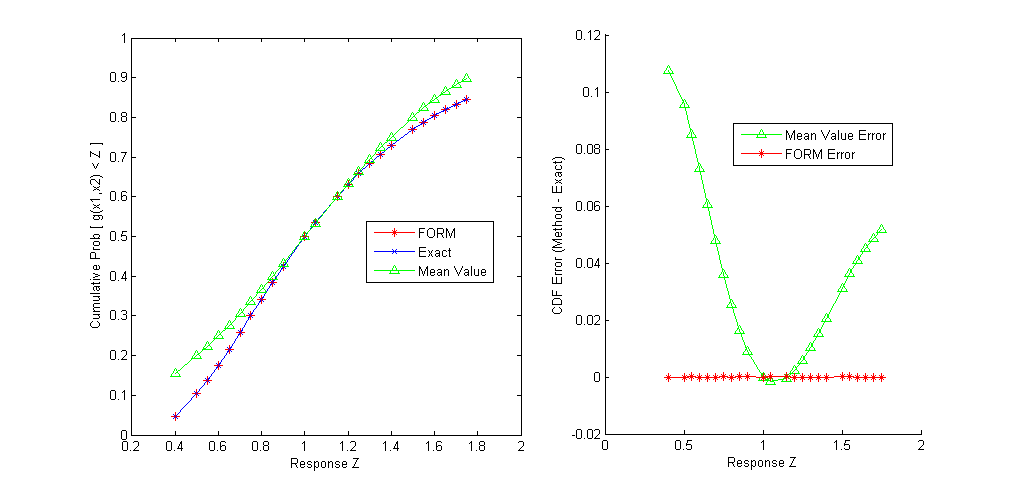
\includegraphics[scale=0.5]{images/cdf_form}
\caption{Comparison of the cumulative distribution function (CDF) computed by
FORM, the Mean Value method, and the exact CDF for $g(x_1,x_2)=\frac{x_1}{x_2}$}
\label{uq:rel_form_compare}
\end{figure}

If the user specifies \texttt{local\_reliability} as a method with no
additional specification on how to do the MPP search (for example, by
commenting out {\tt mpp\_search no\_approx} in
Figure~\ref{uq:rel_input_form}), then no MPP search is done: the Mean
Value method is used. The mean value results are shown in
Figure~\ref{uq:rel_output_mv} and consist of approximate mean and
standard deviation of the response, the importance factors for each
uncertain variable, and approximate probability/reliability levels for
the prescribed response levels that have been inferred from the
approximate mean and standard deviation (see Mean Value section in
Reliability Methods Chapter of Dakota Theory
Manual~\cite{TheoMan}). It is evident that the statistics are
considerably different from the fully converged FORM results; however,
these rough approximations are also much less expensive to
calculate. The importance factors are a measure of the sensitivity of
the response function(s) to the uncertain input variables. A
comparison of the mean value results with the FORM results is shown in
Figure~\ref{uq:rel_form_compare}. The mean value results are not
accurate near the tail values of the CDF, and can differ from the
exact solution by as much as 0.11 in CDF estimates. A comprehensive
comparison of various reliability methods applied to the logratio
problem is provided in ~\cite{Eld06a}.

\begin{figure}[htbp!]
\begin{bigbox}
\begin{small}
\begin{verbatim}
MV Statistics for response_fn_1:
  Approximate Mean Response                  =  1.0000000000e+00
  Approximate Standard Deviation of Response =  5.9160798127e-01
  Importance Factor for TF1ln                =  7.1428570714e-01
  Importance Factor for TF2ln                =  7.1428572143e-01
  Importance Factor for TF1ln     TF2ln      = -4.2857142857e-01
Cumulative Distribution Function (CDF) for response_fn_1:
     Response Level  Probability Level  Reliability Index  General Rel Index
     --------------  -----------------  -----------------  -----------------
   4.0000000000e-01   1.5524721837e-01   1.0141851006e+00   1.0141851006e+00
   5.0000000000e-01   1.9901236093e-01   8.4515425050e-01   8.4515425050e-01
   5.5000000000e-01   2.2343641149e-01   7.6063882545e-01   7.6063882545e-01
   6.0000000000e-01   2.4948115037e-01   6.7612340040e-01   6.7612340040e-01
   6.5000000000e-01   2.7705656603e-01   5.9160797535e-01   5.9160797535e-01
   7.0000000000e-01   3.0604494093e-01   5.0709255030e-01   5.0709255030e-01
   7.5000000000e-01   3.3630190949e-01   4.2257712525e-01   4.2257712525e-01
   8.0000000000e-01   3.6765834596e-01   3.3806170020e-01   3.3806170020e-01
   8.5000000000e-01   3.9992305332e-01   2.5354627515e-01   2.5354627515e-01
   9.0000000000e-01   4.3288618783e-01   1.6903085010e-01   1.6903085010e-01
   1.0000000000e+00   5.0000000000e-01   0.0000000000e+00   0.0000000000e+00
   1.0500000000e+00   5.3367668035e-01  -8.4515425050e-02  -8.4515425050e-02
   1.1500000000e+00   6.0007694668e-01  -2.5354627515e-01  -2.5354627515e-01
   1.2000000000e+00   6.3234165404e-01  -3.3806170020e-01  -3.3806170020e-01
   1.2500000000e+00   6.6369809051e-01  -4.2257712525e-01  -4.2257712525e-01
   1.3000000000e+00   6.9395505907e-01  -5.0709255030e-01  -5.0709255030e-01
   1.3500000000e+00   7.2294343397e-01  -5.9160797535e-01  -5.9160797535e-01
   1.4000000000e+00   7.5051884963e-01  -6.7612340040e-01  -6.7612340040e-01
   1.5000000000e+00   8.0098763907e-01  -8.4515425050e-01  -8.4515425050e-01
   1.5500000000e+00   8.2372893005e-01  -9.2966967555e-01  -9.2966967555e-01
   1.6000000000e+00   8.4475278163e-01  -1.0141851006e+00  -1.0141851006e+00
   1.6500000000e+00   8.6405064339e-01  -1.0987005257e+00  -1.0987005257e+00
   1.7000000000e+00   8.8163821351e-01  -1.1832159507e+00  -1.1832159507e+00
   1.7500000000e+00   8.9755305196e-01  -1.2677313758e+00  -1.2677313758e+00
\end{verbatim}
\end{small}
\end{bigbox}
\caption{Output from Reliability UQ example using mean value.}
\label{uq:rel_output_mv}
\end{figure}

Additional reliability analysis and design results are provided in 
Sections~\ref{additional:logratio}-\ref{additional:steel_column}.


\section{Stochastic Expansion Methods}\label{uq:expansion}


%The objective of these techniques is to characterize the response of
%systems whose governing equations involve stochastic coefficients. 
The development of these techniques mirrors that of deterministic
finite element analysis through the utilization of the concepts of
projection, orthogonality, and weak convergence. The polynomial chaos
expansion is based on a multidimensional orthogonal polynomial
approximation and the stochastic collocation approach is based on a
multidimensional interpolation polynomial approximation, both formed
in terms of standardized random variables. A distinguishing feature of
these two methodologies is that the final solution is expressed as a
functional mapping, and not merely as a set of statistics as is the
case for many other methodologies (sampling, reliability, et al.).
This makes these techniques particularly attractive for use in
multi-physics applications which link different analysis packages.
The first stochastic expansion method is the polynomial chaos
expansion (PCE)~\cite{Gha99,Gha91}. For smooth functions (i.e.,
analytic, infinitely-differentiable) in $L^2$ (i.e., possessing finite
variance), exponential convergence rates can be obtained under order
refinement for integrated statistical quantities of interest such as
mean, variance, and probability. Dakota implements the generalized PCE
approach using the Wiener-Askey scheme~\cite{XiuKarn02}, in which
Hermite, Legendre, Laguerre, Jacobi, and generalized Laguerre
orthogonal polynomials are used for modeling the effect of continuous
random variables described by normal, uniform, exponential, beta, and
gamma probability distributions, respectively\footnote{Orthogonal
polynomial selections also exist for discrete probability
distributions, but are not yet supported in Dakota.}. These orthogonal
polynomial selections are optimal for these distribution types since
the inner product weighting function corresponds\footnote{Identical
support range; weight differs by at most a constant factor.} to the
probability density functions for these continuous
distributions. Orthogonal polynomials can be computed for any positive
weight function, so these five classical orthogonal polynomials may be
augmented with numerically-generated polynomials for other probability
distributions (e.g., for lognormal, extreme value, and histogram
distributions).  When independent standard random variables are used
(or computed through transformation), the variable expansions are
uncoupled, allowing the polynomial orthogonality properties to be
applied on a per-dimension basis. This allows one to mix and match the
polynomial basis used for each variable without interference with the
spectral projection scheme for the response.

In non-intrusive PCE, simulations are used as black boxes and the
calculation of chaos expansion coefficients for response metrics of
interest is based on a set of simulation response evaluations. To
calculate these response PCE coefficients, two classes of
approaches are available: spectral projection and regression. The
spectral projection approach projects the response against each basis
function using inner products and employs the polynomial orthogonality
properties to extract each coefficient. Each inner product involves a
multidimensional integral over the support range of the weighting
function, which can be evaluated numerically using sampling,
tensor-product quadrature, Smolyak sparse grid~\cite{Smolyak_63}, or
cubature~\cite{stroud} approaches. The regression approach finds a set
of PCE coefficients which best match a set of response values obtained
from either a design of computer experiments (``point
collocation''~\cite{pt_colloc1}) or from a randomly selected subset of
tensor Gauss points (``probabilistic
collocation''~\cite{Tat95}). Various methods can be used to solve the
resulting linear system, including least squares methods for
over-determined systems and compressed sensing methods for
under-determined systems. Details of these methods are documented in
the Linear regression section of the Dakota Theory
Manual~\cite{TheoMan} and the necessary specifications needed to
activate these techniques are listed in the keyword section of the
Dakota Reference Manual~\cite{RefMan}.

Stochastic collocation (SC) is another stochastic expansion technique
for UQ that is closely related to PCE. As for PCE, exponential
convergence rates can be obtained under order refinement for
integrated statistical quantities of interest, provided that the
response functions are smooth with finite variance. The primary
distinction is that, whereas PCE estimates coefficients for known
multivariate orthogonal polynomial basis functions, SC forms
multivariate interpolation polynomial basis functions for known
coefficients.  The interpolation polynomials may be either local or
global and either value-based or gradient-enhanced (four combinations:
Lagrange interpolation, Hermite interpolation, piecewise linear
spline, and piecewise cubic spline), and may be used within nodal or
hierarchical interpolation formulations. Interpolation is performed on
structured grids such as tensor-product or sparse grids. Starting from
a tensor-product multidimensional interpolation polynomial in the
value-based case (Lagrange or piecewise linear spline), we have the
feature that the $i^{th}$ interpolation polynomial has a value of 1 at
collocation point $i$ and a value of 0 for all other collocation
points, leading to the use of expansion coefficients that are just the
response values at each of the collocation points. In the
gradient-enhanced case (Hermite or piecewise cubic spline), SC
includes both ``type 1'' and ``type 2'' interpolation polynomials,
where the former interpolate the values while producing zero gradients
and the latter interpolate the gradients while producing zero values
(refer to~\cite{TheoMan} for additional details). Sparse interpolants
are weighted sums of these tensor interpolants;
%and retain the use of response values as expansion coefficients;
however, they are only interpolatory for sparse grids based on fully 
nested rules and will exhibit some interpolation error at the 
collocation points for sparse grids based on non-nested rules.
A key to maximizing performance with SC is performing collocation
using the Gauss points and weights from the same optimal orthogonal
polynomials used in PCE. 
For use of standard Gauss integration rules (not nested variants such
as Gauss-Patterson or Genz-Keister) within tensor-product quadrature,
tensor PCE expansions and tensor SC interpolants are equivalent in
that identical polynomial approximations are
generated~\cite{ConstTPQ}. Moreover, this equivalence can be extended
to sparse grids based on standard Gauss rules, provided that a sparse
PCE is formed based on a weighted sum of tensor expansions~\cite{ConstSSG}.

The Dakota Theory Manual~\cite{TheoMan} provides full algorithmic
details for the PCE and SC methods.

A recent addition is functional tensor train (FTT) expansions which
leverage concepts from data/image compression using products of
dimensional basis ``cores.''  When the response admits a ``low rank''
representation, this means that the size of the cores required for an
accurate recovery is not large and a compressed format for the
expansion can be achieved based on a tensor train composition.  In
Dakota, the basis functions used within the core for each random
dimension are univariate orthogonal polynomials, similar to PCE.
Solution for the expansion coefficients is based on regression and
employs a numerical solution of a regularized nonlinear least squares
problem.  Both the rank and polynomial order per dimension are
resolution controls for the method, and cross-validation procedures
are provided to automate the selection of the best settings for a
given response data set.  Additional FTT theory will be provided in
future releases as this capability is promoted to a default part of
the Dakota software configuration.

Finally, advanced multilevel and multifidelity approaches are
provided for PCE, SC, and FT, as described in the Reference
Manual~\cite{RefMan} (refer to {\tt multilevel\_polynomial\_chaos,
  multifidelity\_polynomial\_chaos, multilevel\_function\_train,
  multifidelity\_function\_train} and {\tt
  multifidelity\_stoch\_collocation}).  These approaches decompose
the input-output mapping and form multiple expansions in order to
reduce reliance on the most expensive computational models
by integrating information from low cost modeling alternatives.
%rich information coming from low cost approximate models and sparse
%information coming from expensive high-fidelity models.

\subsection{Uncertainty Quantification Examples using Stochastic Expansions} \label{uq:stoch_exp:ex}

\subsubsection{Polynomial Chaos Expansion for Rosenbrock}
\label{uq:stoch_exp:ex:pce}

%The term ``Polynomial Chaos'' refers to the representation of a stochastic 
%process as a polynomial expansion in random (or stochastic) variables. This 
%representation acts as a response surface that maps stochastic inputs to 
%stochastic outputs. Desired statistics can then be obtained from the 
%response surface either analytically or by re-sampling the fast surrogate.
%Additional details regarding the method are provided in

A typical Dakota input file for performing an uncertainty
quantification using PCE is shown in
Figure~\ref{uq:examples:pce_input}.  In this example, we compute CDF
probabilities for six response levels of Rosenbrock's function. Since
Rosenbrock is a fourth order polynomial and we employ a fourth-order
expansion using an optimal basis (Legendre for uniform random
variables), we can readily obtain a polynomial expansion which exactly
matches the Rosenbrock function. In this example, we select Gaussian
quadratures using an anisotropic approach (fifth-order quadrature in
$x_1$ and third-order quadrature in $x_2$), resulting in a total of 15
function evaluations to compute the PCE coefficients.

\begin{figure}[htbp!]
  \centering
  \begin{bigbox}
    \begin{small}
      \verbatimtabinput[8]{../../test/examples-users/rosen_uq_pce.in}
    \end{small}
  \end{bigbox}
\caption{Dakota input file for performing UQ using polynomial chaos expansions --
see \protect\path{dakota/share/dakota/examples/users/rosen_uq_pce.in} }
\label{uq:examples:pce_input}
\end{figure}

The tensor product quadature points upon which the expansion is calculated 
are shown in Figure~\ref{uq:examples:rosen_pce_points}. 
The tensor product generates
all combinations of values from each individual dimension: it is an 
all-way pairing of points.

\begin{figure}[htbp!]
  \centering
  \includegraphics[height=2.5in]{images/rosen_pce_pts}
  \caption{Rosenbrock polynomial chaos example: tensor product quadrature points.}
  \label{uq:examples:rosen_pce_points}
\end{figure}

Once the expansion coefficients have been calculated, some statistics
are available analytically and others must be evaluated numerically.
For the numerical portion, the input file specifies the use of 10000
samples, which will be evaluated on the expansion to compute the CDF
probabilities. In Figure~\ref{uq:examples:pce_out}, excerpts from the
results summary are presented, where we first see a summary of the PCE
coefficients which exactly reproduce Rosenbrock for a Legendre
polynomial basis. The analytic statistics for mean, standard
deviation, and COV are then presented. For example, the mean is 455.66
and the standard deviation is 606.56. The moments are followed by
global sensitivity indices (Sobol' indices).This example shows that
variable x1 has the largest main effect (0.497) as compared with
variable x2 (0.296) or the interaction between x1 and x2 (0.206).
After the global sensitivity indices, the local sensitivities are
presented, evaluated at the mean values.  Finally, we see the
numerical results for the CDF probabilities based on 10000 samples
performed on the expansion. For example, the probability that the
Rosenbrock function is less than 100 over these two uncertain
variables is 0.342. Note that this is a very similar estimate to what
was obtained using 200 Monte Carlo samples, with fewer true function
evaluations.
\begin{figure}[htbp!]
\centering
\begin{bigbox}
%\begin{footnotesize}
\begin{scriptsize}
\begin{verbatim}
Polynomial Chaos coefficients for response_fn_1:
        coefficient   u1   u2
        ----------- ---- ----
   4.5566666667e+02   P0   P0
  -4.0000000000e+00   P1   P0
   9.1695238095e+02   P2   P0
  -9.9475983006e-14   P3   P0
   3.6571428571e+02   P4   P0
  -5.3333333333e+02   P0   P1
  -3.9968028887e-14   P1   P1
  -1.0666666667e+03   P2   P1
  -3.3573144265e-13   P3   P1
   1.2829737273e-12   P4   P1
   2.6666666667e+02   P0   P2
   2.2648549702e-13   P1   P2
   4.8849813084e-13   P2   P2
   2.8754776338e-13   P3   P2
  -2.8477220582e-13   P4   P2
-------------------------------------------------------------------
Statistics derived analytically from polynomial expansion:

Moment-based statistics for each response function:
                            Mean           Std Dev          Skewness          Kurtosis
response_fn_1
  expansion:    4.5566666667e+02  6.0656024184e+02
  numerical:    4.5566666667e+02  6.0656024184e+02  1.9633285271e+00  3.3633861456e+00

Covariance among response functions:
[[  3.6791532698e+05 ]] 

Local sensitivities for each response function evaluated at uncertain variable means:
response_fn_1:
 [ -2.0000000000e+00  2.4055757386e-13 ] 

Global sensitivity indices for each response function:
response_fn_1 Sobol indices:
                                  Main             Total
                      4.9746891383e-01  7.0363551328e-01 x1
                      2.9636448672e-01  5.0253108617e-01 x2
                           Interaction
                      2.0616659946e-01 x1 x2 

Statistics based on 10000 samples performed on polynomial expansion:

Probability Density Function (PDF) histograms for each response function:
PDF for response_fn_1:
          Bin Lower          Bin Upper      Density Value
          ---------          ---------      -------------
   6.8311107124e-03   1.0000000000e-01   2.0393073423e-02
   1.0000000000e-01   1.0000000000e+00   1.3000000000e-02
   1.0000000000e+00   5.0000000000e+01   4.7000000000e-03
   5.0000000000e+01   1.0000000000e+02   1.9680000000e-03
   1.0000000000e+02   5.0000000000e+02   9.2150000000e-04
   5.0000000000e+02   1.0000000000e+03   2.8300000000e-04
   1.0000000000e+03   3.5755437782e+03   5.7308286215e-05

Level mappings for each response function:
Cumulative Distribution Function (CDF) for response_fn_1:
     Response Level  Probability Level  Reliability Index  General Rel Index
     --------------  -----------------  -----------------  -----------------
   1.0000000000e-01   1.9000000000e-03
   1.0000000000e+00   1.3600000000e-02
   5.0000000000e+01   2.4390000000e-01
   1.0000000000e+02   3.4230000000e-01
   5.0000000000e+02   7.1090000000e-01
   1.0000000000e+03   8.5240000000e-01
-------------------------------------------------------------------
\end{verbatim}
\end{scriptsize}
%\end{footnotesize}
\end{bigbox}
\caption{Excerpt of UQ output for polynomial chaos example.}
\label{uq:examples:pce_out}
\end{figure}

\subsubsection{Uncertainty Quantification Example using Stochastic Collocation}
\label{uq:stoch_exp:ex:sc}

%A typical Dakota input file for performing an uncertainty
%quantification using polynomial chaos expansions is shown in
%Section~\ref{uq:stoch_exp:ex:pce}, which illustrates PCE defined from an
%anisotropic tensor-product quadrature grid. The uncertain variables
%are uniforms, so the expansion is built using classical Legendre
%polynomials. 

Compared to the previous PCE example, this section presents a more
sophisticated example, where we use stochastic collocation built on an
anisotropic sparse grid defined from numerically-generated orthogonal
polynomials. The uncertain variables are lognormal in this example and
the orthogonal polynomials are generated from Gauss-Wigert recursion
coefficients~\cite{simpson_gw} in combination with the Golub-Welsch
procedure~\cite{GolubWelsch69}.  The input file is shown in
Figure~\ref{uq:figure11}.  Note that the dimension preference of
$(2,1)$ is inverted to define a $\gamma$ weighting vector of $(0.5,1)$
(and $\underline{\gamma}$ of $0.5$) for use in the anisotropic Smolyak
index set constraint (see Smolyak sparse grids section in Stochastic
Expansion Methods chapter in Dakota Theory Manual~\cite{TheoMan}). In
this example, we compute CDF probabilities for six response levels of
Rosenbrock's function. This example requires 19 function evaluations
to calculate the interpolating polynomials in stochastic collocation
and the resulting expansion exactly reproduces Rosenbrock's function.
The placement of the points generated by the sparse grid is shown in
Figure~\ref{uq:figure11b}.

\begin{figure}[htbp!]
  \centering
  \begin{bigbox}
    \begin{small}
      \verbatimtabinput[8]{../../test/examples-users/rosen_uq_sc.in}
    \end{small}
  \end{bigbox}
\caption{Dakota input file for performing UQ using stochastic collocation --
see \protect\path{dakota/share/dakota/examples/users/rosen_uq_sc.in} }
\label{uq:figure11}
\end{figure}

\begin{figure}[htbp!]
  \centering
  \includegraphics[height=2.5in]{images/rosen_sc_pts}
  \caption{Rosenbrock stochastic collocation example: sparse grid points.}
  \label{uq:figure11b}
\end{figure}

Once the expansion coefficients have been calculated, some statistics
are available analytically and others must be evaluated numerically.
For the numerical portion, the input file specifies the use of 10000
samples, which will be evaluated on the expansion to compute the CDF
probabilities. In Figure~\ref{uq:figure12}, excerpts from the results
summary are presented. We first see the moment statistics for mean,
standard deviation, skewness, and kurtosis computed by numerical
integration (see Analytic moments section in Stochastic Expansion
Methods chapter in Dakota Theory Manual~\cite{TheoMan}), where the
numerical row corresponds to integration using the original response
values and the expansion row corresponds to integration using values
from the interpolant. The response covariance (collapsing to a single
variance value for one response function) and global sensitivity
indices (Sobol' indices) are presented next. This example shows that
variable x1 has the largest main effect (0.99) as compared with
variable x2 (0.0007) or the interaction between x1 and x2 (0.005).
%After the global sensitivity indices, the local, analytic random 
%variable sensitivities are presented, as computed from
%Eqs.~\ref{eq:dR_dx}-\ref{eq:dR_dxi_sc}, evaluated at the mean values.
Finally, we see the numerical results for the CDF probabilities based
on 10000 samples performed on the expansion. For example, the probability 
that the Rosenbrock function is less than 100 is 0.7233. Note that these 
results are significantly different than the ones presented in 
Section~\ref{uq:stoch_exp:ex:pce} because of 
the different assumptions about the inputs: uniform[-2,2] versus
lognormals with means of 1.0 and standard deviations of 0.5. 
\begin{figure}[htbp!]
\centering
\begin{bigbox}
\begin{footnotesize}
\begin{verbatim}
Statistics derived analytically from polynomial expansion:

Moment-based statistics for each response function:
                            Mean           Std Dev          Skewness          Kurtosis
response_fn_1
  expansion:    2.5671972656e+02  2.0484189184e+03  2.7419241630e+02  1.9594567379e+06
  numerical:    2.5671972656e+02  2.0484189184e+03  2.7419241630e+02  1.9594567379e+06

Covariance among response functions:
[[  4.1960200651e+06 ]] 

Global sensitivity indices for each response function:
response_fn_1 Sobol indices:
                                  Main             Total
                      9.9391978710e-01  9.9928724777e-01 x1
                      7.1275222945e-04  6.0802128961e-03 x2
                           Interaction
                      5.3674606667e-03 x1 x2 

Statistics based on 10000 samples performed on polynomial expansion:

Level mappings for each response function:
Cumulative Distribution Function (CDF) for response_fn_1:
     Response Level  Probability Level  Reliability Index  General Rel Index
     --------------  -----------------  -----------------  -----------------
   1.0000000000e-01   1.8100000000e-02
   1.0000000000e+00   8.7800000000e-02
   5.0000000000e+01   5.8410000000e-01
   1.0000000000e+02   7.2330000000e-01
   5.0000000000e+02   9.2010000000e-01
   1.0000000000e+03   9.5660000000e-01
\end{verbatim}
\end{footnotesize}
\end{bigbox}
\caption{Excerpt of UQ output for stochastic collocation example.}
\label{uq:figure12}
\end{figure}

\section{Importance Sampling Methods}\label{uq:importance}

Importance sampling is a method that allows one to estimate statistical
quantities such as failure probabilities (e.g. the probability that
a response quantity will exceed a threshold or fall below a threshold value)
in a way that is more efficient than Monte Carlo sampling. The core idea
in importance sampling is that one generates samples that preferentially
samples important regions in the space (e.g. in or near the failure region
or user-defined region of interest), and then appropriately weights
the samples to obtain an unbiased estimate of the failure probability
~\cite{Srinivasan2002}.
In importance sampling, the samples are generated from a density which is
called the importance density:  it is not the original probability density
of the input distributions. The importance density should be centered near the
failure region of interest. For black-box simulations such as those commonly
interfaced with Dakota, it is difficult to specify the importance density a priori:
the user often does not know where the failure region lies, especially in a high-dimensional
space.~\cite{Swiler2010}

More formally, we define the objective of importance sampling as calculating the probability, $P$, that the output will exceed a threshold level. This is a failure 
probability, where the failure probability is defined as some scalar function, 
$y\left(\textbf{X}\right)$, exceeding a threshold, $T$, 
where the inputs, $\textbf{X}$, are randomly distributed with density, $\rho\left(\textbf{X}\right)$. 
When evaluating $y\left(\textbf{X}\right)$ is sufficiently expensive or $P$ is sufficiently small, Monte Carlo (MC) sampling methods to estimate $P$ will be infeasible due to the large number of function evaluations required
for a specified accuracy. 

The probability of failure can be thought of as the mean rate of occurrence
of failure. The Monte Carlo (MC) estimate of $P$ is therefore the sample
mean of the indicator function, $I\left(\textbf{X}\right)$,
\begin{equation}
P_{MC}=\frac{1}{N}\sum_{i=1}^{N}I\left(\mathbf{X_i}\right)\ \ \textbf{X}\sim \rho\left(\textbf{X}\right),
\label{mc_ind}
\end{equation}
where $N$ samples, $\mathbf{X_i}$, are drawn from
$\rho\left(\textbf{X}\right)$,
and the indicator function $I\left(\textbf{X}\right)$
is 1 if failure occurs and zero otherwise.

Importance sampling draws samples from the importance density 
$\rho'\left(\textbf{X}\right)$ and scales the sample mean by the importance density:
\begin{equation}
P_{IS}=\frac{1}{N}\sum_{i=1}^N \left(I\left(\mathbf{X_i}\right)\frac{\rho\left(\mathbf{X_i}\right)}{\rho'\left(\mathbf{X_i}\right)}\right)\ \ \textbf{X}\sim\rho'\left(\textbf{X}\right).\label{eqn:ispfail}
\end{equation}
This reduces the asymptotic error variance from:
\begin{equation}
\sigma_{err_{MC}}^2=\frac{{\rm E}\left[\left(I\left(\textbf{X}\right)-P\right)^2\right]}{N}
\end{equation}
to
\begin{equation}
\sigma_{err_{IS}}^2=\frac{{\rm E}\left[\left(I\left(\textbf{X}\right)\frac{\rho\left(\textbf{X}\right)}{\rho'\left(\textbf{X}\right)}
-P\right)^2\right]}{N}.
\label{eqn:iserrorvar}
\end{equation}
Inspection of Eq. ~\ref{eqn:iserrorvar} reveals $\sigma_{err_{IS}}^2=0$ if
$\rho'\left(\textbf{X}\right)$ equals the ideal importance density
$\rho^*\left(\textbf{X}\right)$,
\begin{equation}
\rho^*\left(\textbf{X}\right)=\frac{I\left(\textbf{X}\right)\rho\left(\textbf{X}\right)}{P}.\end{equation}
 
However, $\rho^*\left(\textbf{X}\right)$ is unknown a priori because
$I\left(\textbf{X}\right)$ is only known where it has been evaluated. 
Therefore, the required $P$ in the denominator is also unknown:  this is what we are trying to estimate.
 
If importance sampling is to be effective, the practitioner must be able to
choose a good $\rho'\left(\textbf{X}\right)$ without already knowing
$I\left(\textbf{X}\right)$ everywhere. 
There is a danger: a poor choice for $\rho'\left(\textbf{X}\right)$ can put most of the samples in
unimportant regions and make $\sigma_{err_{IS}}^2$ much greater than
$\sigma_{err_{MC}}^2$.
In particular, importance sampling can be challenging for very low probability events in high-dimensional spaces where
the output $y$ is calculated by a simulation. In these cases, usually one
does not know anything a priori about where the failure region exists
in input space. 
We have developed two importance sampling approaches which do not
rely on the user explicitly specifying an importance density.

\subsection{Importance Sampling Method based on Reliability Approach}\label{uq:importance_rel}
The first method is based on ideas in reliability modeling ~\ref{uq:reliability:local}.
An initial Latin Hypercube sampling is performed to generate an initial set of samples.
These initial samples are augmented with samples from an importance density as follows:
The variables are transformed to standard normal space. In the transformed space,
the importance density is a set of normal densities centered around points which
are in the failure region. Note that this is similar in spirit to the reliability
methods, in which importance sampling is centered around a Most Probable Point (MPP).
In the case of the LHS samples, the importance sampling density will simply by
a mixture of normal distributions centered around points in the failure region.

This method is specified by the keyword \texttt{importance\_sampling}.
The options for importance sampling are as follows:  \texttt{import} 
centers a sampling
density at one of the initial LHS samples identified in the failure region.
It then generates the importance samples, weights them by their probability of occurence
given the original density, and calculates the required probability (CDF or CCDF level).
\texttt{adapt\_import} is the same as \texttt{import} but is performed iteratively until the
failure probability estimate converges.
\texttt{mm\_adapt\_import} starts with all of the samples located in the failure region
to build a multimodal sampling density. First, it uses a small number of samples around
each of the initial samples in the failure region. Note that these samples
are allocated to the different points based on their relative probabilities of occurrence:
more probable points get more samples. This early part of the approach is done to 
search for ``representative'' points. Once these are located, the multimodal sampling density is set and then the multi-modal adaptive method proceeds similarly to the 
adaptive method (sample until convergence).
 
\subsection{Gaussian Process Adaptive Importance Sampling Method}\label{uq:gpais}
The second importance sampling method in Dakota is the one we recommend,
at least for problems that have a relatively small number of input variables (e.g.
less than 10). This method, Gaussian Process Adaptive Importance Sampling,
is outlined in the paper ~\cite{Dalbey2014}.
This method  starts with an initial set of LHS samples and adds samples one at a time, 
with the goal of adaptively improving the estimate of the ideal importance density
during the process. The approach uses a mixture of component densities. An
iterative process is used
to construct the sequence of improving component densities. At each
iteration, a Gaussian process (GP) surrogate is used to help identify areas
in the space where failure is likely to occur. The GPs are not used to
directly calculate the failure probability; they are only used to approximate
the importance density. Thus, the Gaussian process adaptive importance
sampling algorithm overcomes limitations involving using a potentially
inaccurate surrogate model directly in importance sampling calculations.

This method is specified with the keyword \texttt{gpais}. There are three 
main controls which govern the behavior of the algorithm. 
\texttt{samples} specifies the initial number of Latin Hypercube samples 
which are used to create the initial Gaussian process surrogate. 
\texttt{emulator\_samples} specifies the number of samples taken on the 
latest Gaussian process model each iteration of the algorithm. 
These samples are used in the construction of the next importance 
sampling density. The default is 10,000 samples. The third control 
is \texttt{max\_iterations}, which controls the number of iterations 
of the algorithm. Each iteration, one additional sample of the ``true'' 
simulation is taken. Thus, if \texttt{samples} were set at 100 and 
\texttt{max\_iterations} were set to 200, there would be a total of 
300 function evaluations of the simulator model taken. 

\section{Adaptive Sampling Methods}\label{uq:adaptive}
The goal in performing adaptive sampling is to construct a surrogate model that
can be used as an accurate predictor to some expensive simulation, thus it is
to one's advantage to build a surrogate that minimizes the error over the entire
domain of interest using as little data as possible from the expensive
simulation. The adaptive part alludes to the fact that the surrogate will be
refined by focusing samples of the expensive simulation on particular areas of
interest rather than rely on random selection or standard space-filling
techniques. 

\subsection{Adaptive sampling based on surrogates}\label{uq:adaptive:surrogate}

At a high-level, the adaptive sampling pipeline is a four-step process:
\begin{enumerate}
\item Evaluate the expensive simulation (referred to as the true model) at
initial sample points
\item Fit/refit a surrogate model
\item Create a candidate set and score based on information from surrogate
\item Select a candidate point to evaluate the true model and Repeat 2-4
\end{enumerate}

In terms of the Dakota implementation, the adaptive sampling method 
currently uses Latin Hypercube sampling (LHS) to generate the initial 
points in Step 1 above. For Step 2, we use a Gaussian process model. 
The user can specify the scoring metric used to select the 
next point (or points) to evaluate and add to the set. 
We have investigated several scoring metrics with which to evaluate 
candidate points for Step 3. There are some classical ones such as distance 
(e.g. add a point which maximizes the minimum distance to all of 
the existing points). This distance metric tends to generate 
points that are space-filling. We have investigated several 
methods that involve interesting topological features of the 
space (e.g. points that are near saddle points). These are 
an area of active investigation but are not currently included 
in Dakota. The fitness metrics for scoring 
candidate points currently include: 
\begin{description}
\item[Predicted Variance]
First introduced in \cite{MacKay} and later
used in \cite{Seo}, this method uses the predicted
variance of the Gaussian process surrogate as the score of a candidate 
point. Thus, the adaptively chosen points will be in areas of highest 
uncertainty according to the Gaussian process model.
\item[Distance]
A candidate's score is the Euclidean distance in domain space between the
candidate and its nearest neighbor in the set of points already evaluated on the
true model. Therefore, the most undersampled area of the domain will always be
selected. The adaptivity of this method could be brought to question as it would
chose the exact same points regardless of the surrogate model used. However, it
is useful to use to compare other adaptive metrics to one that relies purely on
space-filling in an equivalent context.
\item[Gradient]
%DPM: PROBABLY WANT TO CHANGE THE NAME OF THIS METRIC
Similar to the above metric, a candidate's nearest neighbor is determined as in
the distance metric, only now the score is the absolute value of the difference
in range space of the two points. The range space values used are predicted
from the surrogate model. Though this method is called the gradient metric, it
actually does not take into account how close the candidate and its neighbor are
in domain space. This method attempts to evenly fill the range space of the
surrogate.
\end{description}

Note that in our approach, a Latin Hypercube sample is generated (a new one, 
different from the initial sample) and the surrogate model is evaluated 
at this points. These are the ``candidate points'' that are then evaluated 
according to the fitness metric outlined above. The number of candidates used 
in practice should be high enough to fill most
of the input domain: we recommend at least hundreds of points for a low-
dimensional problem. 
All of the candidates (samples on the emulator) are 
given a score and then the highest-scoring candidate is selected to be evaluated
on the true model. 

The adaptive sampling method also can generate batches of points 
to add at a time. With batch or  multi-point 
selection, the true model can be evaluated in parallel and thus
increase throughput before refitting our surrogate model. This proposes a new
challenge as the problem of choosing a single point and choosing multiple points
off a surrogate are fundamentally different. Selecting the $n$ best scoring
candidates is more than likely to generate a set of points clustered in one
area which will not be conducive to adapting the surrogate.
We have implemented several strategies for batch selection of points: 
\begin{description}
\item[\bf Naive Selection]  
This strategy will select the $n$ highest scoring candidates regardless of their
position. This tends to group an entire round of points in the same area.
\item[\bf Distance Penalized Re-weighted Scoring] 
In this strategy, the highest 
scoring candidate is selected and then all
remaining candidates are re-scored with a distance penalization factor added in
to the score. Only points selected within a round are used for the distance
penalization. The factor is the same as used in the distance penalization
 scoring metrics from \cite{Maljovec}. First, compute all of the minimum
distances from each remaining candidate to the selected candidates. Then,
determine the median value of these distances. If the smallest distance, $d$,
between a point and the selected set is less than the computed median distance
its score is unaltered, otherwise the score is multiplied by a value $\rho$
determined by the following equation:
\begin{equation}
\rho = 1.5*d - 0.5*d^3
\end{equation}
\item[\bf Topological Maxima of Scoring Function]  
In this strategy we look at the topology of the scoring function and select the
$n$ highest maxima in the topology. To determine local maxima, we construct the
approximate Morse-Smale complex. If the number of local maxima is less than $n$,
 we revert to the distance strategy above. As a further extension, one may
want to filter low-persistence maxima, but to keep the framework general, we
chose to omit this feature as defining a threshold for what deems a critical
point as "low persistence" can vary drastically from problem to problem.
\item[\bf Constant Liar]  
We adapt the constant liar strategy presented in \cite{Ginsbourger} with the
scoring metrics. The strategy first selects
the highest scoring candidate, and then refits the surrogate using a ``lie'' value
at the point selected and repeating until $n$ points have been selected
whereupon the lie values are removed from the surrogate and the selected points
are evaluated on the true model and the surrogate is refit with these values.
\end{description}

The adaptive sampling method is specified by the method keyword 
\texttt{adaptive\_sampling}. There are many controls, including 
the number of candidate samples to investigate each iteration 
(\texttt{emulator\_samples}), the fitness metric used in scoring 
candidates (\texttt{fitness\_metric}), and the number of iterations 
to perform the adaptive sampling (\texttt{max\_iterations}). 
For batch selection of points, one specifies a \texttt{batch\_selection} 
strategy and a \texttt{batch\_size}. 
The details of the specification are provided in the Dakota 
reference manual. 

\subsection{Adaptive sampling based on dart throwing}\label{uq:adaptive:darts}
\texttt{pof\_darts} is a novel method for estimating the tail probability
(Probability of Failure) based on random sphere-packing in the uncertain
parameter space. Random points are sequentially sampled from the domain and
consequently surrounded by protecting spheres, with the constraint that each new
sphere center has to be outside all prior spheres~\cite{ebeida2016pof}. The
radius of each sphere is chosen such that the entire sphere lies either in the
failure or the non-failure region. This radius depends of the function
evaluation at the disk center, the failure threshold and an estimate of the
function gradient at the disk center. After exhausting the sampling budget
specified by \texttt{build\_samples}, which is the number of spheres per failure
threshold, the domain is decomposed into two regions.  These regions correspond
to failure and non-failure categories, each represented by the union of the
spheres of each type. The volume of the union of failure spheres gives a lower
bound on the required estimate of the probability of failure, while the volume
of the union of the non-failure spheres subtracted from the volume of the domain
gives an upper estimate. After all the spheres are constructed, we construct a
surrogate model, specified via a \texttt{model\_pointer}, and sample the
surrogate model extensively to estimate the probability of failure for each
threshold. 

\texttt{pof\_darts} handles multiple response functions and allows each to have
multiple failure thresholds. For each failure threshold \texttt{pof\_darts} will
insert a number of spheres specified by the user-input parameter "samples".
However, estimating the probability of failure for each failure threshold would
utilize the total number of disks sampled for all failure thresholds. For each
failure threshold, the sphere radii changes to generate the right spatial
decomposition. The POF-Darts method is specified by the method keyword
\texttt{pof\_darts}. The sample budget is specified by \texttt{build\_samples}.
By default, the method employs a local approach to estimate the Lipschitz
constant per sphere.
%The method can generally support local or global approaches to estimate the
%Lipschitz constant per sphere, given by (\texttt{lipschitz local} or
%\texttt{lipschitz global}). However, only the local approach is currently
%supported and is the default if not specified by the user.

The surrogate model used by the \texttt{pof\_darts} method for extensive
sampling is specified using a \texttt{model\_pointer}, and its parameters are
therefore defined in that model. It can typically be any global surrogate in
Dakota (e.g., Gaussian process, polynomial chaos expansion, polynomial
regression, etc). POF-Darts can also use piecewise-decomposed surrogates which
build local pieces of the surrogate over different domain patches. The piecewise
decomposition option is a new capability added to Dakota to help construct
surrogates in high-dimensional spaces, using known function evaluations as well
as gradient and Hessian information, if available. The piecewise decomposition
option is declared using the keyword \texttt{domain\_decomp} and currently
supports polynomial, Gaussian Process (GP), and Radial Basis Functions (RBF)
surroagte models only. For example: a polynomial regression global surrogate is
specified with \texttt{model polynomial}, its order is selected using
\texttt{surrogate\_order}, and the piecewise decomposition option is specified
with \texttt{domain\_decomp}. The \texttt{domain\_decomp} option is parametrized
by a \texttt{cell\_type} set by default to Voronoi cells, an optional number of
\texttt{support\_layers}, and an optional \texttt{discontinuity\_detection}
capability. See~\ref{models:surf:piecewise_decomp} for more details.

\section{Epistemic Nondeterministic Methods}\label{uq:epistemic}

Uncertainty quantification is often used as part of the risk
assessment of performance, reliability, and safety of engineered
systems. Increasingly, uncertainty is separated into two categories
for analysis purposes: aleatory and epistemic
uncertainty~\cite{Obe03,Hel07}. Aleatory uncertainty is also referred to as
variability, irreducible or inherent uncertainty, or uncertainty due
to chance. Examples of aleatory uncertainty include the height of
individuals in a population, or the temperature in a processing
environment. Aleatory uncertainty is usually modeled with probability
distributions, and sampling methods such as Latin Hypercube sampling
in Dakota can be used to model aleatory uncertainty. In contrast,
epistemic uncertainty refers to lack of knowledge or lack of
information about a particular aspect of the simulation model,
including the system and environment being modeled. An increase in
knowledge or information relating to epistemic uncertainty will lead
to a reduction in the predicted uncertainty of the system response or
performance. For epistemic uncertain variables, typically one does not
know enough to specify a probability distribution on a variable.
Epistemic uncertainty is referred to as subjective, reducible, or lack
of knowledge uncertainty. Examples of epistemic uncertainty include
little or no experimental data for a fixed but unknown physical
parameter, incomplete understanding of complex physical phenomena,
uncertainty about the correct model form to use, etc.

There are many approaches which have been developed to model epistemic
uncertainty, including fuzzy set theory, possibility theory, and
evidence theory. It is also possible to use simple interval analysis in 
an epistemic context. Interval analysis and evidence theory are 
described in more detail below.

\subsection{Interval Methods for Epistemic Analysis}\label{uq:interval}

In interval analysis, one assumes that nothing is known about 
an epistemic uncertain variable except that its value lies 
somewhere within an interval. In this situation, it is NOT 
assumed that the value has a uniform probability of occuring 
within the interval. Instead, the interpretation is that 
any value within the interval is a possible value or a potential 
realization of that variable. In interval analysis, the 
uncertainty quantification problem is one of determining the 
resulting bounds on the output (defining the output interval) 
given interval bounds on the inputs. Again, any output response 
that falls within the output interval is a possible output 
with no frequency information assigned to it.

We have the capability to perform interval analysis using either
\dakotakw{global_interval_est} or \dakotakw{local_interval_est}.  In
the global approach, one uses either a global optimization method or a
sampling method to assess the bounds.  \texttt{global\_interval\_est}
allows the user to specify either \texttt{lhs}, which performs Latin
Hypercube Sampling and takes the minimum and maximum of the samples as
the bounds (no optimization is performed) or \texttt{ego}. In the case
of \texttt{ego}, the efficient global optimization method is used to
calculate bounds. The ego method is described in
Section~\ref{opt:methods:gradientfree:global}.  If the problem is
amenable to local optimization methods (e.g. can provide derivatives
or use finite difference method to calculate derivatives), then one
can use local methods to calculate these
bounds. \texttt{local\_interval\_est} allows the user to specify
either \texttt{sqp} which is sequential quadratic programming, or
\texttt{nip} which is a nonlinear interior point method.

Note that when performing interval analysis, it is necessary to define
interval uncertain variables as described in
Section~\ref{variables:uncertain}. For interval analysis, one must
define only one interval per input variable, in contrast with
Dempster-Shafer evidence theory, where an input can have several
possible intervals. Interval analysis can be considered a special
case of Dempster-Shafer evidence theory where each input is defined by
one input interval with a basic probability assignment of one. In
Dakota, however, the methods are separate and semantic differences
exist in the output presentation. If you are performing a pure
interval analysis, we recommend using either
\texttt{global\_interval\_est} or \texttt{local\_interval\_est}
instead of \texttt{global\_evidence} or \texttt{local\_evidence}, for
reasons of simplicity. %An example of interval estimation is found in
%the \path{dakota/share/dakota/examples/users/cantilever_uq_global_interval.in},
%and also in Section~\ref{uq:examples:interval}.

%Note that we have kept separate implementations of interval analysis and
%Dempster-Shafer evidence theory because our users often want to couple
%interval analysis on an ``outer loop'' with an aleatory, probabilistic
%analysis on an ``inner loop'' for nested, second-order probability
%calculations. See Section~\ref{adv_models:mixed_uq} for additional
%details on these nested approaches.
These interval methods can also be used as the outer loop within an
interval-valued probability analysis for propagating mixed aleatory
and epistemic uncertainty -- refer to
Section~\ref{adv_models:mixed_uq:ivp} for additional details.

%\subsubsection{Interval Analysis for Cantilever}\label{uq:examples:interval}

%Interval analysis is often used to model epistemic uncertainty. 
%In interval analysis, the 
%uncertainty quantification problem is one of determining the 
%resulting bounds on the output (defining the output interval) 
%given interval bounds on the inputs. 

%We can do interval analysis using either
%\texttt{global\_interval\_est} or \texttt{local\_interval\_est}.
%In the global approach, one uses either a global optimization 
%method or a sampling method to assess the bounds, whereas the 
%local method uses gradient information in a derivative-based 
%optimization approach. 
 
An example of interval estimation 
is shown in Figure~\ref{uq:examples:interval_input}, with example results in 
Figure~\ref{uq:examples:interval_out}. This example is a demonstration 
of calculating interval bounds for three outputs of the cantilever beam 
problem. The cantilever beam problem is described in detail in 
Section~\ref{additional:cantilever}. Given input intervals of [1,10] on 
beam width and beam thickness, we can see that the interval estimate of 
beam weight is approximately [1,100].

\begin{figure}[htbp!]
  \centering
  \begin{bigbox}
    \begin{small}
      \verbatimtabinput[8]{../../test/examples-users/cantilever_uq_global_interval.in}
    \end{small}
  \end{bigbox}
\caption{Dakota input file for performing UQ using interval analysis --
see \protect\path{dakota/share/dakota/examples/users/cantilever_uq_global_interval.in} }
\label{uq:examples:interval_input}
\end{figure}

\begin{figure}[htbp!]
\centering
\begin{bigbox}
\begin{small}
\begin{verbatim}
------------------------------------------------------------------
Min and Max estimated values for each response function:
weight:  Min = 1.0000169352e+00  Max = 9.9999491948e+01
stress:  Min = -9.7749994284e-01  Max = 2.1499428450e+01
displ:  Min = -9.9315672724e-01  Max = 6.7429714485e+01
-----------------------------------------------------------------
\end{verbatim}
\end{small}
\end{bigbox}
\caption{Excerpt of UQ output for interval example.}
\label{uq:examples:interval_out}
\end{figure}


\subsection{Dempster-Shafer Theory of Evidence}\label{uq:dempshaf}

We have chosen to pursue evidence theory at Sandia as a way to model
epistemic uncertainty, in part because evidence theory is a
generalization of probability theory. Evidence theory is also
referred to as Dempster-Shafer theory or the theory of random
sets~\cite{Obe03}. This section focuses on the use of Dempster-Shafer
evidence theory for propagating epistemic uncertainties. When
aleatory uncertainties are also present, we may choose either to
discretize the aleatory probability distributions into sets of
intervals and treat them as well-characterized epistemic variables, or
we may choose to segregate the aleatory uncertainties and treat them
within an inner loop. A nested Dempster-Shafer approach for
propagating mixed aleatory and epistemic uncertainty is described in
Section~\ref{adv_models:mixed_uq:dste}.
%We also use a technique called second-order probability to perform
%uncertainty quantification when there is both epistemic and aleatory
%uncertainty present. Second-order probability is a nested technique
%with two levels of uncertainty quantification. The outer level UQ is
%typically linked to epistemic uncertainties and the inner level UQ is
%commonly associated with aleatory uncertainties. A common approach
%used is to sample possible realizations of epistemic variables in the
%outer loop, then send these to the inner loop for additional sampling
%over the aleatory variables. In this way one generates ``families''
%or ensembles of cumulative distribution functions, where each
%individual CDF is based on aleatory uncertainty, and the ensemble is
%based on epistemic uncertainty. See Section~\ref{adv_models:mixed_uq}
%for more details.

In evidence theory, there are two complementary measures of
uncertainty: belief and plausibility. Together, belief and
plausibility can be thought of as defining lower and upper bounds,
respectively, on probabilities. Belief and plausibility define the
lower and upper limits or intervals on probability values. Typical
plots of cumulative and complementary cumulative belief and
plausibility functions are shown in Figure~\ref{uq:figure15}~\cite{Hel07}.
\begin{figure}[htbp!]
  \centering 
  \includegraphics[scale=0.8]{images/belief_plaus} 
  \caption{Example cumulative belief and plausibility distribution functions on left; complementary cumulative belief and plausibility distribution functions on right}
  \label{uq:figure15}
\end{figure}
In evidence theory, it is not possible to specify one probability value.
Instead, there is a range of values that is consistent with the
evidence. The range of values is defined by belief and
plausibility. Note that no statement or claim is made about one value
within an interval being more or less likely than any other value.

In Dempster-Shafer evidence theory, the uncertain input variables are
modeled as sets of intervals. The user assigns a basic probability
assignment (BPA) to each interval, indicating how likely it is that
the uncertain input falls within the interval. The BPAs for a
particular uncertain input variable must sum to one. The intervals
may be overlapping, contiguous, or have gaps. In Dakota, an interval
uncertain variable is specified as \dakotakw{interval_uncertain}. When
one defines an interval type variable in Dakota, it is also necessary
to specify the number of intervals defined for each variable with
\dakotakw{iuv_num_intervals} as well the basic probability assignments
per interval, \dakotakw{iuv_interval_probs}, and the associated bounds
per each interval, \dakotakw{iuv_interval_bounds}. 
Figure~\ref{uq:figure16} shows the input specification for interval
uncertain variables. 
The example has two epistemic uncertain interval variables. 
The first uncertain
variable has three intervals and the second has two. The basic
probability assignments for the first variable are 0.5, 0.1, and 0.4,
while the BPAs for the second variable are 0.7 and 0.3. Note that it
is possible (and often the case) to define an interval uncertain
variable with only ONE interval. This means that you only know that
the possible value of that variable falls within the interval, and the
BPA for that interval would be 1.0. In the case we have shown, the
interval bounds on the first interval for the first variable are 0.6
and 0.9, and the bounds for the second interval for the first variable
are 0.1 to 0.5, etc.

\begin{figure}[htbp!]
  \centering
  \begin{bigbox}
    \begin{small}
      \verbatimtabinput[8]{../../test/examples-users/textbook_uq_glob_evidence.in}
    \end{small}
  \end{bigbox}
\caption{Dakota input file for UQ example using Evidence Theory --
see \protect\path{dakota/share/dakota/examples/users/textbook_uq_glob_evidence.in} }
\label{uq:figure16}
\end{figure}

Once the intervals, the BPAs, and the interval bounds are defined, 
the user can run an epistemic analysis by specifying the method as 
either \texttt{global\_evidence} or 
\texttt{local\_evidence} in the Dakota input file. 
Both of these methods perform Dempster-Shafer calculations:  
the difference is that the local method uses a local optimization 
algorithm to calculate the interval bounds and the global 
method uses either sampling or a global optimization approach to 
calculate an interval bound. These differences are discussed in 
more detail below. 
The intervals and their associated BPAs are then propagated through
the simulation to obtain cumulative distribution functions on belief
and plausibility. As mentioned above, belief is the lower bound on a
probability estimate that is consistent with the evidence, and
plausibility is the upper bound on a probability estimate that is
consistent with the evidence. 

Figure~\ref{uq:figure17} shows
results for the first response function obtained when running the
example in Figure~\ref{uq:figure16}. In this example, there are 6
output intervals (as a result of the 2 interval input variables with 3
and 2 intervals, respectively). 
The output intervals are ordered to obtain cumulative
bound functions for both belief and plausibility. The
cumulative distribution function is presented for both belief (CBF) and
plausibility (CPF). The CBF value is the cumulative belief
corresponding to a certain output value. For example, the belief that
the output value is less than or equal to 0.2 for response 1 is 0.27, 
and the plausibility that the output is less than
or equal to 0.2 is 1 for response 1. The belief that the 
output value is less than 0.6217 is 0.75, while the plausbility that 
the output is less than  0.0806 is 0.75. 
The CBF and CPF may be plotted on a graph and
interpreted as bounding the cumulative distribution
function (CDF), which is the probability that the output is less than or equal
to a certain value. The interval bounds on probability values show
the value of epistemic uncertainty analysis: the intervals are usually
much larger than expected, giving one a truer picture of the total
output uncertainty caused by lack of knowledge or information about
the epistemic input quantities.

\begin{figure}[htbp!]
\centering
\begin{bigbox}
\begin{small}
\begin{verbatim}
Belief and Plausibility for each response function:
Cumulative Belief/Plausibility Functions (CBF/CPF) for response_fn_1:
     Response Level  Belief Prob Level   Plaus Prob Level
     --------------  -----------------   ----------------
   1.0000000000e-03   0.0000000000e+00   0.0000000000e+00
   3.0000000000e-02   0.0000000000e+00   2.7000000000e-01
   2.0000000000e-01   2.7000000000e-01   1.0000000000e+00
   8.0000000000e-01   9.3000000000e-01   1.0000000000e+00
  Probability Level  Belief Resp Level   Plaus Resp Level
  -----------------  -----------------   ----------------
   2.5000000000e-01   2.6187288772e-01   6.2609206069e-02
   5.0000000000e-01   2.9829775860e-01   6.3736734971e-02
   7.5000000000e-01   6.2173551556e-01   8.0596931719e-02
\end{verbatim}
\end{small}
\end{bigbox}
\caption{Results of an Epistemic Uncertainty Quantification using Evidence Theory.}
\label{uq:figure17}
\end{figure}

As in other nondeterministic methods, with \texttt{local\_evidence}
or \texttt{global\_evidence},
one can specify probability levels and response levels. 
If response levels are specified, the belief and plausibility 
function values corresponding to those response levels are calculated 
(see Belief Prob Level and Plaus Prob Level in the tables shown in 
Figure~\ref{uq:figure17}). Similarly, if probability levels are 
specified, these are first interpreted to be belief values, and the 
corresponding response levels are calculated (see Belief Resp Level); 
then they are interpreted to be plausibility values and the 
corresponding response levels are calculated (see Plaus Resp Level in 
the table in Figure~\ref{uq:figure17}). We have recently added the 
capability to support generalized reliability mappings in 
the evidence methods. If the user specifies a generalized 
reliability level, it will be first converted to a probability, 
then interpreted as a belief and plausibility and the corresponding 
response levels will be calculated. Likewise, if response levels 
are specified, the corresponding belief and plausibility values 
will be mapped to bounds on the generalized reliability levels. 

To elaborate on the differences between \texttt{global\_evidence} and
\texttt{local\_evidence}: both of these methods take the
Dempster-Shafer structures specified on the inputs and calculate a
resulting Dempster-Shafer structure on the outputs (e.g. a cumulative
belief and plausibility function).  To calculate the belief and
plausibility measures, it is necessary to calculate the minimum and
maximum of the response function in each ``interval cell
combination.''  For example, in a two variable problem, if the first
variable had three intervals and associated BPAs assigned and the
second variable had two intervals and associated BPAs assigned, there
would be 6 interval cells in total.  In each of these six cells, one
needs to identify a minimum and maximum value of the response
function. This is easy to do if the function is monotonic in both
variables, but in general it is not. We offer the capability to use
local optimization methods to calculate these bounds:
\texttt{local\_evidence} allows the user to specify either
\texttt{sqp} which is sequential quadratic programming, or
\texttt{nip} which is a nonlinear interior point method. We also offer
the capability to use global methods to assess these interval cell
bounds. \texttt{global\_evidence} allows the user to specify either
\texttt{lhs}, which performs Latin Hypercube Sampling and takes the
minimum and maximum of the samples within each cell as the bounds (no
optimization is performed) or \texttt{ego}. In the case of
\texttt{ego}, the efficient global optimization method is used to
calculate bounds. The \texttt{ego} method is described in
Section~\ref{opt:methods:gradientfree:global}.  Note that for a
situation with many uncertain variables, each with a fairly
complicated Dempster-Shafer structure described by many intervals,
there will be a huge number of interval calls, and the overall process
of performing Dempster-Shafer analysis will be extremely expensive.
Reference~\cite{Tang10b} provides more details about the
implementation of the optimization methods to perform Dempster-Shafer
calculations, as well as comparisons on test problems.

\section{Bayesian Calibration Methods}\label{uq:bayesian}

In Bayesian calibration a ``prior distribution'' on a parameter is
updated through a Bayesian framework involving experimental data and a
likelihood function.  Bayesian inference theory is best left to other
sources ~\cite{Kenn01} and only a brief summary is given here.  In
Bayesian methods, uncertain parameters are characterized by
probability density functions. These probability density functions
define the permissible parameter values - the support, as well as the
relative plausibility of each permissible parameter value. In the
context of calibration or any inference step, the probability density
function that describes knowledge before the incorporation of data is
called the prior, $f_{\boldsymbol{\Theta}}\left( \boldsymbol{\theta}
\right)$.
 
Note: In Dakota, the prior distribution is characterized by the
properties of the active uncertain variables. Correlated priors are
only supported for unbounded normal, untruncated lognormal, uniform,
exponential, gumbel, frechet, and weibull distributions and require a
probability transformation by specifying
\dakotakw{standardized_space}.

When data are available, the likelihood function describes how well
each parameter value is supported by the data. Bayes
Theorem~\cite{Jaynes}, shown in Equation~\ref{eq:BayesThm}, is used
for inference: to derive the plausible parameter values, based on the
prior probability density and the data $\boldsymbol{d}$. The result is
the posterior probability density function of the parameters
$f_{\boldsymbol{{\Theta |D}}}\left( \boldsymbol{{\theta |d}}
\right)$. It is interpreted the same way as the prior, but includes
the information derived from the data.
 
\begin{equation}
{f_{\boldsymbol{\Theta |D}}}\left( \boldsymbol{\theta |d} \right) = \frac{{{f_{\boldsymbol{\Theta}}}\left( \boldsymbol{\theta}  \right)\mathcal{L}\left( \boldsymbol{\theta;d} \right)}}{{{f_{\boldsymbol{D}}}\left( \boldsymbol{d} \right)}}. \label{eq:BayesThm}
\end{equation}


%\begin{equation}
%  \label{eqn:BayesThm}
%  {f_{\Theta |D}}\left( {\theta |d} \right) = \frac{{{f_\Theta }\left( \theta  \right)\mathcal{L}\left( {\theta ;d} \right)}}{{{f_D}\left( d \right)}}
%\end{equation}

The likelihood function is used to describe how well a model's
predictions are supported by the data.  The likelihood function can be
written generally as:
\begin{equation*}
  \mathcal{L}\left(\boldsymbol{{\theta ;d}} \right) =  \mathcal{F}(q(\boldsymbol{\theta)} -\boldsymbol{d}),
\end{equation*}
where $\boldsymbol{\theta}$ are the parameters of model quantity of
interest $q$.  The form of the function $\mathcal{F}$ can greatly
influence the results.  The specific likelihood function used in
Dakota is based on Gaussian probability density functions. This means
that we assume the difference between the model quantity
(e.g. quantity of interest returned from a computer simulation) and
the experimental observations are Gaussian:
\begin{equation}\label{eq:model}
d_i = q_i(\boldsymbol{\theta}) + \epsilon_i,
\end{equation}
where $\epsilon_i$ is a random variable that can encompass both
measurement errors on $d_i$ and modeling errors associated with the
simulation quantity of interest $q_i$, for each of $n$ observations.

If we assume that all experiments and observations are independent,
then the probabilistic model defined by Eq.~(\ref{eq:model}) results
in a likelihood function for $\boldsymbol{\theta}$ that is the product
of $n$ normal probability density functions:
%as shown in Equation~\ref{eqn:Likelihood}.
\begin{equation}\label{eqn:Likelihood}  
\mathcal{L}(\boldsymbol{{\theta};d}) = \prod_{i=1}^n
\frac{1}{\sigma_d \sqrt{2\pi}} \exp
\left[ - \frac{\left(d_i-q_i(\boldsymbol{{\theta}})\right)^2}{2{\sigma_d}^2} \right],
%\mathcal{L}\left( {{\theta};d} \right) = \prod\limits_{i = 1}^n {\frac{1}{{\sigma \sqrt {2\pi } }}  \exp \left[  - \frac{\left(d_i - \mathcal{M}({\theta})\right)^2}{2\sigma^2} \right]
\end{equation}
where ${\sigma_d}^2$ refers to the measurement error of the data,
assumed constant across all data observations in this case.

We also support the more general case of a full covariance matrix,
$\boldsymbol{\Sigma_d}$, that specifies the covariance between each
observation $i$ and $j$.  In this case, the likelihood is commonly
written in log form, where the log-likelihood
is: %given in Equation~\ref{eqn:LogLikelihood}.
\begin{equation}\label{eqn:LogLikelihood}  
\log{\mathcal{L}(\boldsymbol{{\theta};d})} \propto % =-0.5 {R}^{T} {\Sigma_d}^{-1} {R}
-\frac{1}{2} \boldsymbol{r}^T \boldsymbol{\Sigma_d}^{-1} \boldsymbol{r},
\end{equation}
where $\boldsymbol{r}$ is the vector of residuals between the data
points and the model quantity of interest,
$q(\boldsymbol{\theta})-\boldsymbol{d}$.

Dakota admits four \texttt{experiment\_variance\_type} options to specify the
measurement error covariance: \texttt{none} for no measurement error
specified (in this case, the variance is assumed to be one),
\texttt{scalar} where a constant value ${\sigma_d}^2$ is given for all
observations, \texttt{diagonal} where a value is specified for the
diagonal elements of the covariance matrix $\boldsymbol{\Sigma_d}$
meaning that each observation has its own measurement error but there
are no cross terms, and \texttt{matrix} where the full covariance
matrix $\boldsymbol{\Sigma_d}$ is specified.  The \texttt{diagonal}
and \texttt{matrix} terms are only available for field response data.
In contrast to earlier versions of Dakota, all measurement error
variance should be specified with units of variance/covariance, not
standard deviation.

Markov Chain Monte Carlo (MCMC) is the prototypical method used to
estimate posterior parameter densities, given the observational data
and the priors. There are many references that describe the basic
algorithm~\cite{Gilks} and this is an active research area.  MCMC
algorithms may require hundreds of thousands of steps to converge,
depending on dimensionality, response nonlinearity, and the desired
set of posterior statistics.  Since each iteration involves an
evaluation of the model to obtain $q(\boldsymbol{\theta})$, surrogate
models of expensive simulations are often employed to make the MCMC
process tractable.
 
Dakota offers five approaches for Bayesian calibration: QUESO, DREAM,
GPMSA, MUQ, and WASABI.  They are specified with the
\texttt{bayes\_calibration} keyword in combination with the
\texttt{queso}, \texttt{dream}, \texttt{gpmsa}, \texttt{muq}, or \texttt{wasabi}
selections, respectively.  The QUESO and GPMSA methods use components
from the QUESO library (Quantification of Uncertainty for Estimation,
Simulation, and Optimization) developed at The University of Texas at
Austin.  It implements the Delayed Rejection and Adaptive
Metropolis~\cite{Haario} (DRAM) algorithm, among others.  Algorithm
variants selectively combine the delayed rejection and adaptive
elements.  The QUESO/GPMSA capability is based on the GPMSA Matlab
toolbox developed at Los Alamos National Laboratory and uses tightly
integrated Gaussian process models during calibration.  The Dakota
implementation of QUES0/GPMSA is in a prototype stage.  DREAM uses an
implementation of DiffeRential Evolution Adaptive Metropolis developed
by John Burkardt.  The DREAM approach runs concurrent chains for
global exploration, and automatically tunes the proposal covariance
during the process by a self-adaptive randomized subspace
sampling~\cite{Vrugt}. MUQ uses components from the MIT 
Uncertainty Quantification library and also implements the Delayed Rejection
and Adaptive Metropolis~\cite{Haario} (DRAM) algorithms, among others.
The prototype WASABI method is an MCMC-free Bayesian calibration
approach.  QUESO/DRAM and variants are the most well-developed within
Dakota.

\subsection{QUESO}\label{uq:bayesian:queso}
The QUESO library includes several sampling algorithm variants.  One
can use a standard Metropolis-Hastings algorithm
(\texttt{metropolis\_hastings}), adaptive Metropolis
(\texttt{adaptive\_metropolis}) for adapting the proposal covariance
during the sampling, delayed rejection (\texttt{delayed\_rejection})
for backtracking from sample rejections, the full DRAM (\texttt{dram})
which involves both delayed rejection and adaptive Metropolis, or a
multi-level algorithm (\texttt{multilevel}).  This last option is not
yet production-ready in Dakota. 

With any choice of sampling algorithm, one may manually set the burn in 
period for the MCMC chain with \texttt{burn\_in\_samples}. If a 
\texttt{sub\_sampling\_period} is specified, the MCMC chain is further 
filtered such that only the sample at the beginning of each period is in 
the final MCMC chain. The \texttt{sub\_sampling\_period} should therefore 
be greater than or equal to the correlation length of the samples.

With the QUESO method, one may run the MCMC sampling on the simulation
model directly.  However, if the model is expensive, use of a
surrogate (emulator) model is recommended.  Options include a Gaussian
process, a polynomial chaos expansion, or a stochastic collocation
expansion.

The proposal covariance refers to the covariance structure of a
multivariate normal distribution, which governs sample generation in
the chain.  One may specify \texttt{proposal\_covariance}, followed by
\texttt{prior} (the default), \texttt{values}, \texttt{filename}, or
\texttt{derivatives}.  With the \texttt{prior} setting, the proposal
covariance will be set to the variance of the prior distributions of
the parameters being calibrated.  When specifying the proposal
covariance with input file values or from a separate file, the user
may specify only the diagonals of the covariance matrix or the full
covariance matrix.

The derivatives option will use derivatives from the simulation or
emulator model to form or approximate the Hessian of the misfit
function (the negative log likelihood).  Especially when derivative
information is available inexpensively (e.g. from an emulator), the
derivative-based proposal covariance forms a more accurate proposal
distribution, resulting in lower rejection rates and faster chain
mixing.  When using an emulator, the derivative-based proposal
covariance should be updated periodically using the
\texttt{posterior\_adaptive} specification.  This will add simulation
truth evaluations in areas of high-likelihood to the emulator training
data, thus refining the Hessian.  For more detail about
derivative-based formulations involving the misfit Hessian, refer to
the Theory Manual.

An additional control for QUESO is to perform a logit transformation
(\texttt{logit\_transform}) which performs an internal variable
transformation from bounded domains to unbounded
domains. %in order to reduce sample rejection due to an out-of-bounds condition.
This option can be helpful when regions of high posterior density
exist in the corners of a multi-dimensional bounded domain.  In these
cases, it may be difficult to generate feasible samples from the
proposal density, and transformation to unbounded domains may
greatly reduce sample rejection rates.

The \texttt{pre\_solve} option will perform a deterministic
gradient-based optimization before the MCMC sampling to get a good
starting point for the chain.  This pre-solve seeks to maximize the
log-posterior (the log-likelihood minus the log-prior) to identify the
maximum a posteriori probability point, also called the MAP point.
The Markov Chain will then start at the MAP point, which can
circumvent a lot of initial searching for high posterior probability
points.  The pre-solve option can be used with an emulator or with no
emulator.

Credible and prediction intervals will be calculated if 
\texttt{probability\_levels} is specified. Credible intervals propagate 
uncertainties in parameter density information to the quantity of interest
and quantify how well the model fits the provided data, while prediction 
intervals propagate both parameter and experimental measurement uncertainties 
and contain the next experimental or simulated observation with the specified 
probability. Further details can be found in \cite{Smith2013}. If
\texttt{probability\_levels} is specified, credible intervals will always be 
calculated. Prediction intervals will only be calculated if 
\texttt{experiment\_variance\_type} is also specified in the \texttt{responses} 
block. 
By specifying \texttt{posterior\_stats}, information-theoretic metrics may be 
calculated using the posterior distribution of parameters. If the 
\texttt{kl\_divergence} option is selected, the Kullback-Leibler Divergence
will be calculated between the posterior and the prior distributions such that
\begin{equation}
D_{KL} = \int {f_{\boldsymbol{\Theta |D}}}\left( \boldsymbol{\theta |d} \right) 
\log \frac{ {f_{\boldsymbol{\Theta |D}}}\left( \boldsymbol{\theta |d} \right) }
{{f_{\boldsymbol{\Theta}}}\left( \boldsymbol{\theta}  \right)} 
d\boldsymbol{\theta}.
\end{equation} 
This quantity represents the amount of information gained about the parameters
during the Bayesian update. Further details regarding the calculation and use
of $D_{KL}$ can be found in~\cite{TheoMan}.

\subsection{DREAM}
For the DREAM method, one can define the number of chains used with the
\texttt{chains} specification.  The total number of generations per chain in
DREAM is the number of samples divided by the number of chains.
%The minimum number of chains is three.
The number of chains randomly selected to be used in the crossover
each time a crossover occurs is \texttt{crossover\_chain\_pairs}.
There is an extra adaptation during burn-in, in which DREAM estimates a
distribution of crossover probabilities that favors large jumps over
smaller ones in each of the chains.
Normalization is required to ensure that all of the input dimensions contribute
equally.  In this process, a discrete number of candidate points for
each crossover value is generated, which can be specified with \texttt{num\_cr}.
The \texttt{gr\_threshold} control is the convergence tolerance for the Gelman-Rubin
statistic, which governs the convergence of the multiple chain
process.  The integer \texttt{jump\_step} forces a long jump every 
\texttt{jump\_step} generations.
For more details about these parameters, refer to \cite{Vrugt}. 
Credible and prediction intervals can be calculated by specifying
\texttt{probability\_levels}, and statistics regarding the posterior may be
calculated by specifying \texttt{posterior\_stats}, as described in 
Section~\ref{uq:bayesian:queso}. 

\subsection{GPMSA}
Core to GPMSA is the construction of a Gaussian process emulator from
simulation runs collected at various settings of input parameters. The
emulator is a statistical model of the system response, and it is used
to incorporate the observational data to improve system predictions
and constrain or calibrate the unknown parameters. The GPMSA code
draws heavily on the theory developed in the seminal Bayesian
calibration paper by Kennedy and O'Hagan~\cite{Kenn01}. The particular
approach developed by the Los Alamos group, and implemented in QUESO
and therefore Dakota, is provided in~\cite{Hig08}.  It includes an
embedded discrepancy model and the ability to estimate various
hyper-parameters of the Gaussian process, observation error model, and
discrepancy model.  Dakota's GPMSA capability is an experimental
prototype with a number of limitations.  See the Dakota Reference
Manual~\cite{RefMan} for more information.

\subsection{MUQ}
MUQ is the MIT Uncertainty Quantification library.  See
\url{https://bitbucket.org/mituq/muq2/src/master/} and
\url{https://mituq.bitbucket.io/index.html} for additional
documentation.  Dakota currently exposes four MCMC approaches from MUQ:
Metropolis-Hastings, Adaptive Metropolis, Delayed Rejection, and
Delayed-Rejection Adaptive Metropolis. Dakota's MUQ integration
is preliminary, anticipated to extend to use MUQ components for
Hamiltonian Monte Carlo and Langevin-based sampling.  MUQ is an
experimental Dakota capability, and as such, it is not turned on by
default, and must be explicitly enabled when compiling Dakota.

\subsection{WASABI}
WASABI differs from the other Bayesian approaches in that it is 
not an MCMC-based approach.  Instead, it is based on the idea of 
``consistent Bayes'' which is outlined in ~\cite{Butler2017}.
This approach to stochastic inference uses measure-theoretic 
principles to construct a probability measure or density on model parameters
that is consistent with the model and the data.  The idea is that
the probability measure on the parameters, when ``pushed-foward'' through
the computational model, will give results that match the probability 
measure on the observational data.  

We use a similar notation as with the Bayesian methods, but the interpretation 
is different here.  The goal is to identify the posterior density on the 
parameters, $\pi_{post}({\theta})$, which is equal to the prior density on the 
parameters times a ratio.  The numerator of the ratio, $\pi_{D}^{obs}$, 
describes the relative likelihood that the output of the model corresponds 
to the observed data ${D}$:  this is the density of the data evaluated at 
the model output.  
$q(\boldsymbol{\theta})$ refers to the model output.  
$\pi_{D}^{q_{prior}}$ refers to the push-forward of the prior through the model 
and represents a forward propagation of uncertainty. 
\begin{equation}
\pi_{post}(\boldsymbol{\theta})=\pi_{prior}(\boldsymbol{\theta})\frac{\pi_{D}^{obs}(q(\boldsymbol{\theta}))}{\pi_{D}^{q_{prior}}(q(\boldsymbol{\theta}))}. 
\label{eq:consistentBayesEq}
\end{equation}

The Theory Manual~\cite{TheoMan} has more detail about the assumptions and mathematical foundations 
for this method.  Note a major difference in interpretation of the posterior results with respect to 
a standard Bayesian approach:  In a standard Bayesian approach, the posterior reflects an updated state 
of information about the prior distribution on parameter values induced by the observational data.  
In consistent Bayes, the posterior reflects a stochastic mapping of parameter values such that the posterior 
parameters, when pushed-forward through the model, give results that are consistent with the density 
of the observational data. 
WASABI is a prototype capability.  See the Dakota Reference
Manual~\cite{RefMan} for more information.

\subsection{Feature Comparison}
Table~\ref{tab:bayes_comparison} compares the options available 
with the QUESO, DREAM, GPMSA, MUQ, and WASABI implementations in Dakota. 

\begin{table}
\centering
\caption{Capabilities of Bayesian methods in Dakota}
\label{tab:bayes_comparison}
\begin{tabulary}{\textwidth}{|L|C|C|C|C|C|}
\hline
Capability           &  QUESO  & MUQ  & GPMSA & DREAM & WASABI \\
\hline
Prior Distributions  &  Any continuous variable type
                     &  Any continuous variable type
                     &  Any continuous variable type
                     & Uniform only & Uniform only \\
\hline
Inference Type       & MCMC with DR, AM, DRAM, or MH
                     & MCMC with DR, AM, DRAM, or MH
                     & MCMC with DR, AM, DRAM, or MH
                     & MCMC with Differential Evolution Adaptive Metropolis & MCMC-free interval analysis \\
\hline
Can use PCE/SC Emulator        &  Yes            & Yes              & Yes                    & Yes  & Yes \\
\hline
Can use GP Emulator            &  Yes            &  Yes            & Yes (required)  & Yes                    & Yes \\
\hline
Likelihood-based adaptive emulator update  &  Yes            &  No             &  No             & No                     & No \\     
\hline
Initialize with MAP pre-solve  &  Yes            &  Yes            &  No             & No                     & No \\
\hline
Proposal covariance options    &  prior, user, derivative-based    & n/a                    &  prior, user  & n/a                    & n/a \\            
\hline
Can calibrate error covariance multipliers &  Yes            &  Yes            &  Yes (internal) & Yes                    & No          \\                
\hline
Supports standardized space    &  Yes            &  Yes            & Yes             & Yes                    & Yes           \\             
\hline
Logit transform                &  Yes            &  Yes            & Yes             &  No                    & No            \\             
\hline
Posterior export               &  samples        &  samples        & samples         &  samples               & samples, density \\             
\hline
\end{tabulary}
\end{table}


\subsection{Bayesian Calibration Example}\label{uq:bayesian:ex}

To run a QUESO-based Bayesian calibration in Dakota, create a Dakota
input file such as the one shown in Figure~\ref{uq:figure18}.  Here,
the QUESO DRAM (delayed rejection adaptive metropolis) solver is
selected. The number of samples = 1000 indicates how many points to
generate in the acceptance chain\footnote{If delayed rejection is
  active, the number of simulation evaluations will typically be
  higher due to backtracking.}.  This example uses the
\texttt{mod\_cantilever} algebraic model, so an emulator is not
warranted.  The proposal covariance used has diagonal element values
of 1.e6 and 0.1. Two credible and prediction intervals will be
calculated for each model output: a 5/95 interval and a 10/90
interval. The calibration terms in the responses section refers to the
number of outputs that will be used in the calibration process: in
this case, it is just two. The calibration data file has the
observational data: in this case, it is a freeform file (e.g. no
header or annotation) with ten experiments. For each experiment, there
are two experiment values, one for stress and one for displacement,
followed by two variance values for the error associated with that
experiment for each quantity of interest.

\begin{figure}[htbp!]
  \centering
  \begin{bigbox}
    \begin{small}
      \verbatimtabinput[8]{../../test/examples-users/queso_uq.in}
    \end{small}
  \end{bigbox}
  \caption{Dakota input file for Bayesian calibration}
\label{uq:figure18}
\end{figure}

When the input file shown in~\ref{uq:figure18} is run, Dakota will run
the MCMC algorithm and generate a posterior sample of
$\boldsymbol{\theta}$ in accordance with Bayes
Theorem~\ref{eq:BayesThm} and the likelihood
function~\ref{eqn:Likelihood}. Dakota's final output summary reports
an evaluation count summary and the best sample point visited during
the MCMC process as measured by maximum posterior probability (an
estimate of the MAP point).  The final output also summarizes the
moments of the posterior samples from the chain (e.g.  mean of the
chain, standard deviation of the chain samples, etc.), as well as the
credible and prediction intervals for each model output.

Auxilliary output is also generated to a directory called
\path{QuesoDiagnostics/} in the directory from which Dakota is run.
The file \path{display_sub0.txt} contains diagnostic information
regarding the MCMC process.  The Matlab files contained in the
\path{QuesoDiagnostics/} directory contain the chain files.  The
files to load in Matlab are \path{raw_chain.m} or
\path{filtered_chain.m}, containing the full chain or the filtered
chain values of the parameters\footnote{The full chain will be output
  in cases of adaptive posterior refinement or proposal updating,
  since these use cases access the entire acceptance chain to identify
  refinement data or restarting points, respectively.}.  In addition,
the accepted chain values that Dakota generates are written to a file
in the run directory called (by default)
\path{dakota_mcmc_tabular.dat}. The first columns of this file are
the posterior values of the input variables. If \texttt{burn\_in} or
\texttt{sub\_sampling\_period} are specified, the filtered acceptance
chain is instead written to the file
\path{dakota_mcmc_tabular.dat}. This file contains the posterior
values of the filtered MCMC chain, as well as the values of state
variables and the resulting model responses. Finally, if one wants to
see the likelihood of each point, specifying verbose output in the
method section will result in the likelihoods being printed.

\subsection{Chain Diagnostics}

The convergence of the chain produced by MCMC may require many
thousands of steps, if not millions, as discussed earlier in this
section. Assessing the convergence of MCMC chains is an active area of
research, and the implementation of metrics for chain convergence is
undergoing active development in Dakota, and can be triggered during a
Bayesian calibration study through the use of the keyword
\texttt{chain\_diagnostics}. 

As of Dakota 6.10,  \texttt{confidence\_intervals} is the only
diagnostic implemented. 

Suppose $g$ is a function that represents some characteristic (e.g.
moment) of an underlying distribution, such as the mean or variance.
Then under the standard assumptions of an MCMC chain,  the true value
can be approximated by taking the ensemble mean over the MCMC chain.
The confidence interval for the true moment calculated using the
asymptotically valid interval estimator is given by~\cite{Fle10}
\begin{equation}
  \bar{g}_{n} \pm t_{*} \frac{\hat{\sigma}_{n}}{\sqrt{n}},
\end{equation}
where $\bar{g}_{n}$ is the estimated moment (i.e. mean or variance),
$t_{*}$ is the Student's $t$-value for the 95th quantile, $n$ is the
MCMC chain length, and $\hat{\sigma}_{n}$ is an estimate of the
standard error whose square is obtained using batch means estimation.
To obtain the estimate $\hat{\sigma}_{n}$, the Markov chain produced
during calibration is broken up into ``batches," the sample moment is
calculated for each batch, and $\hat{\sigma}_{n}$ is subsequently
obtained as an unbiased estimate of the standard deviation in the
moment calculations over the batches. The confidence intervals
produced are 95\% confidence intervals, and they are calculated for
the mean and variance (first and second moments) for each parameter
and each response. Further details regarding the default settings for
these calculations can be found in the Dakota Theory
Manual~\cite{TheoMan}. 

Confidence intervals may be used as a chain diagnostic by setting
fixed-width stopping rules~\cite{Rob18}. For example, if the interval
width is below some threshold value, that may indicate that enough
samples have been drawn. Common choices for the threshold value
include:
\begin{itemize}
  \item Fixed width: $\epsilon$
  \item Relative magnitude: $\epsilon \| \bar{g}_{n} \|$
  \item Relative standard deviation: $\epsilon \| \hat{\sigma}_{n} \|$
\end{itemize}
If the chosen threshold is exceeded, \texttt{samples} may need to be
increased, say by 10\%, and the diagnostics reevaluated for signs of
chain convergence. Furthermore, if \texttt{output} is set to
\texttt{debug}, the sample moment for each batch (for each parameter
and response) is output to the screen. The user can then analyze the
convergence of these batch means in order to deduce whether the MCMC
chain has converged.

\subsection{Calibrating the Observation Error Model}

As discussed in Section~\ref{input:calib_data}, Dakota accepts user
information on the covariance $\Sigma_d$ among observation errors and
includes this in the likelihood formulation:
\begin{equation*}
\log{\mathcal{L}(\boldsymbol{{\theta};d})} \propto % =-0.5 {R}^{T} {\Sigma_d}^{-1} {R}
-\frac{1}{2} \boldsymbol{r}^T \boldsymbol{\Sigma_d}^{-1} \boldsymbol{r}.
\end{equation*}

In some cases, it can be helpful to fine tune the assumptions in this
covariance during the calibration process.  Dakota supports
calibrating one or more multipliers on the blocks of the error
covariance.  So if $\Sigma_d$ is block diagonal such that $\Sigma_d =
\mbox{diag}({\Sigma_d}_1, ..., {\Sigma_d}_N)$, we instead formulate as
$\Sigma_d = \mbox{diag}(m_1{\Sigma_d}_1, ..., m_P{\Sigma_d}_P)$ and
calibrate the multipliers $m_i$ as hyper-parameters in the Bayesian
inference process.

The supported modes for calibrating observation error multipliers are
shown in Figure \ref{fig:uq:obs_err_mult}: \dakotakw{one},
\dakotakw{per_experiment}, \dakotakw{per_response}, and \dakotakw{both}.
Here, the two major blocks denote two experiments, while the inner
blocks denote five response groups (two scalar, three field).  The
priors on the hyper-parameters $m_i$ are taken to be inverse gamma
distributions, with mean and mode approximately 1.0 and standard
deviation approximately 0.1.

\begin{figure}[htbp!]
  \centering
  \begin{subfigmatrix}{2}
    \subfigure[]{\includegraphics[scale=0.5]{images/CalibrateOne}}
    \subfigure[]{\includegraphics[scale=0.5]{images/CalibratePerExperiment}}
    \subfigure[]{\includegraphics[scale=0.5]{images/CalibratePerResponse}}
    \subfigure[]{\includegraphics[scale=0.5]{images/CalibrateBoth}}
  \end{subfigmatrix}
  \caption{Calibrating observational error covariance multipliers: (a)
    one multiplier on whole user-provided covariance structure, (b)
    multiplier per-experiment, (c) multiplier per-response, and (d)
    both..}
  \label{fig:uq:obs_err_mult}
\end{figure}

\subsection{Scaling and Weighting of Residuals}

Dakota's scaling options, described in
Section~\ref{opt:additional:scaling}, can be used on Bayesian
calibration problems, using the \dakotakw{calibration_term_scales}
keyword, to scale the residuals between the data points and the model
predictions, if desired. Additionally, Bayesian calibration
residuals-squared can be weighted via the \dakotakw{calibration_terms
weights} specification. Neither set of weights nor scales are adjusted
during calibration.  When response scaling is active, it is applied
after error variance weighting and before \dakotakw{weights}
application. The \dakotakw{calibration_terms} keyword documentation in
the Dakota Reference Manual~\cite{RefMan} has more detail about
weighting and scaling of the residual terms.

\subsection{Model Evidence} 
In some situations, there are multiple models that may represent a phenomenon 
and the user is left with the task to determine which is most appropriate given 
the available data. In this case, Bayesian model selection may help.  Suppose that 
the user has a set of models, $\mathcal{M}$={$M_1,M_2...M_m$} from which to 
choose.  In the Bayesian setting, the parameters of each of these models may be 
updated according to Bayes' rule: 
\begin{equation}
\pi_{post}(\boldsymbol{\theta_i}|D,M_i)=\pi_{prior}(\boldsymbol{\theta_i}|M_i)\frac{\pi(D|\boldsymbol{\theta_i},M_i)}{\pi(D|M_i)}
\end{equation}
where the dependence on the model has been made explicit.  The denominator is used
as the likelihood of a specific model of interest in a version of Bayes' rule which calculates 
the posterior model plausibility as: 
\begin{equation}
\pi_{post}(M_i|D)=\pi_{prior}(M_i)\frac{\pi(D|M_i)}{\pi(D)}
\label{eq:model_plausibility}
\end{equation}
In this equation, the posterior model probability given the data is 
also referred to as model plausibility.  The prior model plausibility, 
$\pi(M_i)$, is usually taken to be uniform, meaning equally likely for all 
models, but it does not have to be.  $\pi(D)$ is a normalizing factor such 
that the sum of all model plausibilities is 1.  In this context, model selection 
involves choosing the model with the highest posterior model plausibility. 
Model evidence is defined as the likelihood in 
Equation~\ref{eq:model_plausibility}, denoted by $\pi(D|M_i)$.  Model evidence 
is determined by averaging the likelihood of its model parameters over all possible 
values of the model parameters, according to their prior distributions.  It is 
also called the marginal likelihood of the model.  Model evidence 
is defined as: 
\begin{equation}
\pi(D|M_i)=\int \pi(D|\boldsymbol{\theta_i},M_i)\pi_{prior}(\boldsymbol{\theta_i}|M_i)d \boldsymbol{\theta_i}
\label{eq:uq:model_evidence}
\end{equation}

There are many ways to calculate model evidence. There are currently two methods 
implemented in Dakota. The user first specifies \texttt{model\_evidence}, then either 
\texttt{mc\_approx} and/or \texttt{laplace\_approx} depending on the
method(s) used to calculate model evidence.
\begin{enumerate}
\item Monte Carlo approximation.  This involves sampling from the prior 
distribution of the parameters, calculating the corresponding likelihood values 
at those samples, and  estimating the integral given in Eq.~\ref{eq:uq:model_evidence} 
by brute force.  The number of samples used in the sampling of the integral is 
determined by \dakotakw{evidence_samples}. Although this method is easy, 
it is not efficient because each sample of the prior density requires 
an evaluation of the simulation model to compute the corresponding likelihood.  
Additionally, many prior samples will have very low (near zero) likelihood, 
so millions of samples may be required for accurate computation of the integral. 
\item Laplace approximation.  This approach is based on the Laplace approximation, 
as outlined in~\cite{Wasserman}.  It has the assumption that the posterior distribution 
is nearly Gaussian, which is not always a safe assumption. 
Then, with maximum a posteriori (MAP) point $\hat{\boldsymbol{\theta}}$, 
the Laplace approximation of model evidence is: 
  
\begin{equation}
\int \pi(D|\boldsymbol{\theta_i},M_i)\pi_{prior}(\boldsymbol{\theta_i}|M_i)d \boldsymbol{\theta_i} \approx \pi(D|\hat{\boldsymbol{\theta}},M_i)\pi(\hat{\boldsymbol{\theta}}|M_i)(2\pi)^{N_i/2}{\|\det(H(\hat{\boldsymbol{\theta}}))\|}^{-1/2}
\end{equation}
where $N_i$ is the number of unknown parameters in the i-th model and 
$H$ is the negative Hessian of the log-posterior evaluated at the MAP point 
$\hat{\boldsymbol{\theta}}$. 
Therefore, this implementation only requires the evaluation of the model likelihood 
and the Hessian of the log-posterior density at the MAP point. 

\end{enumerate}

\subsection{Model Discrepancy}
%kam
Whether in a Bayesian setting or otherwise, the goal of model calibration
is to minimize the difference between the observational data $d_i$ and 
the corresponding model response $q_i(\boldsymbol{\theta})$. In the 
presence of scenario or configuration variables $x$, Eq.~\ref{eq:model} can
be modified,
\begin{equation}
d_i(x) = q_i\left(\boldsymbol{\theta}, x\right) + \epsilon_i,
\end{equation} 
with the ensuing equations of the likelihood and Bayes' Theorem updated 
likewise. The configuration variables represent experimental settings, such 
as temperature or pressure, that may vary between experiments. 

However, it is often the case that the agreement between the 
data and the model after calibration is not sufficiently close. This is 
generally attributed to model form or structural error, and can be corrected 
to some extent with the use of model discrepancy. The Kennedy and 
O'Hagan~\cite{Kenn01} formulation takes the form
\begin{equation}
d_i(x) = q_i\left(\boldsymbol{\theta}, x\right) + \delta_i(x) + \epsilon_i,
\end{equation} 
where $\delta_i(x)$ represents the model discrepancy. For scalar responses, the
model discrepancy is \textit{only} a function of the configuration variables.
Furthermore, one discrepancy model is calculated for \textit{each} observable
$d_i$, $i = 1, \ldots, n$, yielding $\delta_1, \ldots, \delta_n$. For field
responses, a single, global $\delta$ is a function of the configuration 
variables as well as the independent field coordinates, which are usually 
points in time or space. The construction of the model discrepancy in cases 
with mixed scalar and field responses has not been tested.

The current implementation of the model discrepancy capability in Dakota 
serves as a post-processing mechanism after the completion of a Bayesian update.
If \texttt{model\_discrepancy} is specified in the input file, Dakota will 
perform the Bayesian update as detailed in the section above, and then begin 
the process of approximating $\delta$. For each scalar observable $d_i$ and for 
each configuration $x_j$,
\begin{equation}
\delta_i \left( x_j \right) = d_i \left( x_j \right) - 
q_i \left(\boldsymbol{\theta}^*, x_j \right),
\end{equation}
where $\boldsymbol{\theta}^*$ is the average of the calibrated posterior 
distribution of the model parameters. The $i^{th}$ discrepancy function
will be built over the computed $\delta_i \left( x_j \right)$, $j = 1, \ldots,
m$. For field observable $d$, the discrepancy is calculated for each
independent field coordinate $t_{i}$ and for each configuration $x_{j}$,
\begin{equation}
  \delta(t_{i}, x_{j}) = d(t_{i}, x_{j}) - q(\boldsymbol{\theta}^{*}, t_{i},
  x_{j}).
\end{equation}
The global discrepancy function is then built over the computed $\delta(t_{i},
x_{j})$, $i = 1, \ldots, n$, $j = 1, \ldots, m$. For simplicity in future
notation, we let $\delta_{i}(x_i) = \delta(t_i, x_i)$.

The field discrepancy function is built using a Gaussian process regression
model with a quadratic trend function. If instead the responses are scalars, 
more options for the regression model are available. Within the Dakota input 
file, the user may specify the \texttt{discrepancy\_type} to be either a 
Gaussian process or polynomial regression model with the 
\texttt{gaussian\_process} or \texttt{polynomial} commands, respectively. 
Additionally, the order of the trend function may be selected using the 
\texttt{correction\_order} command and choosing one of \texttt{constant}, 
\texttt{linear}, or \texttt{quadratic}. Any specifications using these keywords 
will apply to all $\delta_i$. By default, Dakota will build a Gaussian process 
discrepancy model with a quadratic trend function. Information regarding how 
polynomial and Gaussian process models are built can be found in 
Sections~\ref{models:surf:polynomial} and~\ref{models:surf:kriging}, 
respectively. 

The user may specify new ``prediction" configurations at which the 
corrected model should be calculated. For each response and for each new
configuration, $q_i(\boldsymbol{\theta}, x_{k,new}) + \delta_i(x_{k,new})$ 
will be computed. The prediction configurations can be specified in one of
three ways. If \texttt{num\_prediction\_configs} is included, Dakota will 
uniformly distribute the indicated number of prediction configurations 
throughout the domain of the configuration variable that is given in the 
\texttt{variables} block of the input file. Alternatively, the user may 
explicitly list desired prediction configuration locations within the input
file following the \texttt{prediction\_configs} keyword, or in an external
file to be read in with the \texttt{import\_prediction\_configs} option. If 
none of these three options is selected, Dakota will automatically calculate
corrected model predictions at ten configurations in the scalar response case, 
with the predictions spread uniformly in the configuration variable domain. In 
the case of field responses, corrected model predictions are calculated for each
value of the input configuration variable(s).

Calculations corresponding to each prediction configuration and to each
observable will be output to tabular files. The responses from the discrepancy
model itself is output to \path{dakota_discrepancy_tabular.dat}. Those
from the corrected model are output to \path{dakota_corrected_tabular.dat}.
The user may specify the output file names for the discrepancy and corrected
model tabular files using the \texttt{export\_discrepancy\_file} and
\texttt{export\_corrected\_model\_file} keywords, respectively. 

Variance information corresponding to each specified configuration location 
and for each observable is also computed. In a prediction setting for scalar 
responses, the variance calculated from the discrepancy model is additively 
combined with the variance information provided with the experimental data, 
such that
\begin{equation}
\label{eq:discrep_var}
\Sigma_{total,i}(x) = \Sigma_{\delta, i}(x) + \sigma^{2}_{exp,i} I
\end{equation}
for each observable $i$. Further details of how the variance 
$\Sigma_{\delta,i}(x)$ is computed for Gaussian process and polynomial 
regression models can be found in the Dakota Theory Manual~\cite{TheoMan}. The 
experimental variance provided for parameter calibration may vary for the
same observable from experiment to experiment, thus $\sigma^{2}_{exp,i}$ is
taken to be the maximum variance given for each observable. That is,
\begin{equation}
\sigma^2_{exp,i} = \max_{j} \sigma^2_{i}(x_j), 
\end{equation}
where $\sigma^2_{i}(x_j)$ is the variance provided for the $i^{th}$ observable
$d_i$, computed or measured with the configuration variable $x_j$. 

When each corrected model value $q_i(\boldsymbol{\theta}^{*}, x_{k, new}) +
\delta_i(x_{k,new})$ is considered, the variance calculated 
via~\ref{eq:discrep_var} provides a prediction interval, similar to those 
described in Section~\ref{uq:bayesian:queso}. Including $\sigma^{2}_{exp,i}$ 
in the variance calculation accounts for the uncertainty in the model 
predictions that arise due to uncertainties in the calibration data. These
prediction variances are output to the file 
\path{dakota_discrepancy_variance_tabular.dat} by default. The name of
this file can be modified using the \texttt{export\_corrected\_variance\_file} 
keyword in the input script. If the response is a field, the variance 
information written to this file is the variance of the Gaussian process alone.
Future work includes calculation of combined experimental variance and 
discrepancy model variance for field responses.

Additional details and an illustrative example of these calculations are given 
in the Dakota Theory Manual~\cite{TheoMan}.

\subsection{Bayesian Experimental Design}
\label{sec:bayes_expdesign}

The goal of experimental design is to add observational data to the Bayesian
update that informs model parameters and reduces their uncertainties. In 
Bayesian approaches, data from physical experiments is typically used to 
calibrate a model. However, another common practice is to use responses or
output from a high-fidelity model as ``truth data" in place of experimental 
data in a low-fidelity model calibration. This can be done in with a single
Bayesian calibration, or it can be done iteratively with the use of 
experimental design, where an initial set of high-fidelity runs is 
augmented sequentially to find the next ``best" high-fidelity design point at
which to run the high-fidelity model to add to the calibration data. The 
low-fidelity posterior parameter distribution is then updated again using 
Bayesian calibration. The mutual information is used as the selection criterion 
to guide the process of high-fidelity data acquisition.

In Dakota, design conditions, such as temperature or spatial location, can be 
specified using so-called configuration
variables. The design selection algorithm implemented in Dakota uses a 
user-specified high-fidelity code to produce the ``experimental" or 
observational data that is used in the calibration of the desired low-fidelity 
model. The high-fidelity model is dependent only upon the design or 
configuration variables while the low-fidelity model depends on both the 
design variables and uncertain model parameters. 

An example Dakota input file that implements this Bayesian experimental design 
algorithm is shown in 
Figures~\ref{figure:uq_expdesign1}-\ref{figure:uq_expdesign2}. Note that there 
are three \texttt{model} blocks, one describing the model hierarchy and one 
each for the high-fidelity and low-fidelity models. There are two 
\texttt{variables}, \texttt{interface}, and \texttt{responses} blocks such that 
each model has its own specifications. The low-fidelity \texttt{variables} 
block contains information about both the design variables, which are specified 
with \texttt{continuous\_state}, and the parameters to be updated via Bayes' 
Theorem~\ref{eq:BayesThm}, which are specified using one of the aleatory 
uncertain variable types discussed in Section~\ref{variables:uncertain:cauv}. 
In the high-fidelity \texttt{variables} block, only the 
\texttt{continuous\_state} parameters are included. The specifications of the 
design variables should be consistent in both blocks. Each \texttt{interface} 
block should point to the appropriate high- or low-fidelity code, and the 
\texttt{responses} blocks should contain consistent details about the responses 
from each code. For example, both of the models should return the same number 
of \texttt{calibration\_terms}.  

\stepcounter{figure}
\renewcommand{\thelstlisting}{\thechapter.\arabic{figure}}
\lstinputlisting
[
float=htbp,
lastline=53,
caption={Dakota input file for Bayesian Experimental Design.}, 
label={figure:uq_expdesign1},
captionpos=b,
basicstyle=\small,
frame=single
]
{../../test/examples-users/bayes_experimental_design.in}
\stepcounter{figure}
\lstinputlisting
[
float=htbp,
firstline=54,
caption={Dakota input file for Bayesian Experimental Design.}, 
label={figure:uq_expdesign2},
captionpos=b,
basicstyle=\small,
frame=single
]
{../../test/examples-users/bayes_experimental_design.in}

The mutual information experimental design algorithm is selected by specifying 
\texttt{bayesian\_calibration}, \texttt{queso}, and 
\texttt{experimental\_design} within the \texttt{method} block of the input 
file, and the first \texttt{model} block should contain the 
\texttt{hierarchical} specification of the \texttt{surrogate} keyword. The 
algorithm starts by performing a Bayesian calibration using a number of data
points, specified in Dakota by \texttt{initial\_samples}. These initial data
points can be pulled from external data using the 
\texttt{calibration\_data\_file} keyword in the high-fidelity \texttt{response}
block. In this case, \texttt{num\_config\_variables} should be specified and 
set to the number of configuration variables captured in the \texttt{variables} 
blocks. Furthermore, for use in Bayesian experimental design, 
\texttt{calibration\_data\_file} should contain the configuration variables 
and the corresponding high-fidelity model responses. Scalar variance 
information may be included for the calibration data through the use of the 
\texttt{experimental\_variance\_type} or \texttt{simulation\_variance} command 
within the high-fidelity \texttt{responses} block. The former is applied to any 
user-provided data, such as through the \texttt{calibration\_data\_file} 
keyword, while the latter applies only to those high-fidelity model responses 
produced by the high-fidelity code run by Dakota. Further information can be 
found in the Dakota Reference Manual~\cite{RefMan}. If the number of points 
taken from this file is less than \texttt{initial\_samples}, or if no such 
file is provided, Latin Hypercube Sampling is used to draw samples of the 
design space, and the high-fidelity model is run at these points to supplement
the user-specified data. After this initial calibration, a set of design 
conditions (i.e.\ configuration variables) of size \texttt{num\_candidates} is 
proposed. Users may specify these candidate points through the 
\texttt{import\_candidate\_points\_file} command. Again, if the number of 
points in this file is less than \texttt{num\_candidates}, or if no such file 
is provided, Latin Hypercube Sampling is used to draw samples of the design 
space.  

From these candidate designs, that which maximizes the mutual information with
respect to the low-fidelity model parameters is deemed ``optimal." The mutual
information is approximated using the low-fidelity model and a $k$-nearest
neighbor algorithm, as detailed in~\cite{Lew16}. This optimal design is used in 
the high-fidelity model to create a new observation, which is appended to the 
initial data. This updated data is used to recalculate the Bayesian posterior,
and the process repeats until one of three stopping criteria are met.
Multiple optimal designs may be selected concurrently by specifying 
\texttt{batch\_size} in the input script. These designs are selected using
the greedy algorithm described in detail in~\cite{TheoMan}. In this case, the
high-fidelity model is run at all batch-selected optimal designs before the
Bayesian posterior is recalculated with the updated data for an ensuing 
iteration of the experimental design algorithm. 

There are two algorithms that may be used to calculate the mutual information,
both of which are derived in~\cite{Kra04}. The first algorithm discussed 
therein is used as the default algorithm within Dakota; the second may be 
selected by including the keyword \texttt{ksg2} in the Dakota input script. 
Furthermore, the user may choose to include, during the computation of the 
mutual information, a stochastic error term on the low-fidelity model 
responses. This is done by specifying \texttt{simulation\_variance} in the 
\texttt{responses} block corresponding to the low-fidelity model. See the 
Dakota Theory Manual~\cite{TheoMan} for more information regarding the 
implementation of the mutual information calculations.

There are three criteria by which this algorithm is considered complete. 
The user may specify \dakotakw{max_hifi_evaluations}, which limits the number 
of high-fidelity model simulations Dakota will run. Note that this does not 
include any simulations needed to perform the initial Bayesian calibration of 
the low-fidelity model parameters. Alternatively, if the change in the mutual 
information from one iteration to the next is sufficiently small or if all 
candidate points have been exhausted, the algorithm will terminate. 

Progress of the algorithm will be reported to the screen with the rest of the
Dakota output. Furthermore, a summary of the algorithm's results, including, 
for each iteration, the optimal design, the mutual information, and the 
corresponding high-fidelity model response, can be found in the file 
\path{experimental_design_output.txt}.

\subsubsection{One-at-a-time Implementation}

There may be some applications for which the high-fidelity model must be run
independently of Dakota. This algorithm may still be implemented in this case,
however, it requires some extra work by the user to ensure that the 
high-fidelity model information is properly communicated to Dakota, as a 
"dummy" high-fidelity model code must be supplied to Dakota. The data to be 
used in the initial Bayesian calibration should be gathered from the 
high-fidelity model or physical experiment and imported via the 
\texttt{calibration\_data\_file} in the high-fidelity \texttt{responses} block, 
and extra care should be taken to ensure that \texttt{initial\_samples} matches 
the number of experiments in this file. It is also best, for this use-case, to 
use \texttt{import\_candidate\_points\_file}, with \texttt{num\_candidates} 
exactly matching the number of candidate points in the file.

By setting \texttt{max\_hifi\_evaluations} to zero, Dakota will run the initial
calibration of the low-fidelity model, select the optimal design (or multiple
optimal designs when \texttt{batch\_size} is greater than 1) from 
those provided in \texttt{import\_candidate\_points\_file}, and exit 
\textit{without} running the ``dummy" high-fidelity model code. The selected
design(s) will be output to the screen, as well as to 
\path{experimental_design_output.txt}, as detailed above. The high-fidelity
model may then be run offline with the newly selected design point(s).

The user must update \texttt{calibration\_data\_file} with the new 
high-fidelity data when it becomes available, as well as remove the previously
selected design point(s) from \texttt{import\_candidate\_points\_file}. Within 
the Dakota input file, \texttt{initial\_samples}, \texttt{num\_experiments}, 
and \texttt{num\_candidates} should be correspondingly updated. Dakota may then
be run again to yield the next optimal experimental design(s). It should be 
noted that the stopping criteria will not be automatically evaluated by Dakota 
when one-at-a-time implementation is used. The user must determine when the 
algorithm should be terminated.

\section{Uncertainty Quantification Usage Guidelines} \label{usage:uq}

The choice of uncertainty quantification method depends on how the
input uncertainty is characterized, the computational budget, and the
desired output accuracy.  The recommendations for UQ methods are
summarized in Table~\ref{usage:guideuq} and are discussed in the
remainder of the section.

\begin{table}[hbp]
\centering
\caption{Guidelines for UQ method selection.} \label{usage:guideuq}\vspace{2mm}
\begin{tabular}{|c|c|c|}
\hline
\textbf{Method} & \textbf{Desired Problem} & \textbf{Applicable Methods} \\
\textbf{Classification} & \textbf{Characteristics} & \\
\hline
Sampling & nonsmooth, multimodal response functions;       & sampling 
(Monte Carlo or LHS) \\
         & response evaluations are relatively inexpensive & \\
\hline
Local       & smooth, unimodal response functions; & local\_reliability
(MV, AMV/AMV$^2$,\\
reliability & larger sets of random variables;     & AMV+/AMV$^2$+, TANA, 
FORM/SORM) \\
            & estimation of tail probabilities     & \\
\hline
Global      & smooth or limited nonsmooth response; & global\_reliability \\
reliability & multimodal response; low dimensional; & \\
            & estimation of tail probabilities      & \\
\hline
Adaptive    & smooth or limited nonsmooth response; & importance\_sampling, \\
Sampling    & multimodal response; low dimensional; & gpais, adaptive\_sampling, \\
            & estimation of tail probabilities      & pof\_darts \\
\hline
Stochastic & smooth or limited nonsmooth response; & polynomial\_chaos, \\
expansions & multimodal response; low dimensional; & stoch\_collocation\\
           & estimation of moments or moment-based metrics & \\
\hline
Epistemic & uncertainties are poorly characterized &
interval: local\_interval\_est, \\
 & & global\_interval\_est, sampling; \\
 & & BPA: local\_evidence, global\_evidence \\
\hline
Mixed UQ  & some uncertainties are poorly characterized &
nested UQ (IVP, SOP, DSTE) with epistemic \\
 & & outer loop and aleatory inner loop, sampling \\
\hline
\end{tabular}
\end{table}


{\bf Sampling Methods} \\
Sampling-based methods are the most robust uncertainty techniques
available, are applicable to almost all simulations, and possess
rigorous error bounds; consequently, they should be used whenever the
function is relatively inexpensive to compute and adequate sampling
can be performed. In the case of terascale computational simulations,
however, the number of function evaluations required by traditional
techniques such as Monte Carlo and Latin hypercube sampling (LHS)
quickly becomes prohibitive, especially if tail statistics are
needed. %Additional sampling options include quasi-Monte Carlo (QMC)
%sampling and importance sampling (IS),
%or Markov Chain Monte Carlo (MCMC) sampling
%and incremental sampling may also be used to incrementally add samples 
%to an existing sample set.

Alternatively, one can apply the traditional sampling techniques to a
surrogate function approximating the expensive computational
simulation (see Section~\ref{adv_models:sbuq}). However, if this
approach is selected, the user should be aware that it is very
difficult to assess the accuracy of the results obtained. Unlike
the case of surrogate-based local minimization (see
Section~\ref{adv_meth:sbm:sblm}), there is no simple pointwise calculation to
verify the accuracy of the approximate results. This is due to the
functional nature of uncertainty quantification, i.e. the accuracy of
the surrogate over the entire parameter space needs to be considered,
not just around a candidate optimum as in the case of surrogate-based
local. This issue especially manifests itself when trying to estimate
low probability events such as the catastrophic failure of a system.

{\bf Reliability Methods} \\
Local reliability methods (e.g., MV, AMV/AMV$^2$, AMV+/AMV$^2$+, TANA,
and FORM/SORM) are more computationally efficient in general than the
sampling methods and are effective when applied to reasonably
well-behaved response functions; i.e., functions that are smooth,
unimodal, and only mildly nonlinear. They can be used to provide
qualitative sensitivity information concerning which uncertain
variables are important (with relatively few function evaluations), or
compute full cumulative or complementary cumulative response functions
(with additional computational effort). Since they rely on gradient
calculations to compute local optima (most probable points of
failure), they scale well for increasing numbers of random variables,
but issues with nonsmooth, discontinuous, and multimodal response
functions are relevant concerns. In addition, even if there is a
single MPP and it is calculated accurately, first-order and
second-order integrations may fail to accurately capture the shape of
the failure domain. In these cases, adaptive importance sampling
around the MPP can be helpful. Overall, local reliability methods
should be used with some care and their accuracy should be verified
whenever possible.

An effective alternative to local reliability analysis when confronted
with nonsmooth, multimodal, and/or highly nonlinear response functions
is efficient global reliability analysis (EGRA). This technique
employs Gaussian process global surrogate models to accurately resolve
the failure domain and then employs multimodal adaptive importance
sampling to resolve the probabilities. For relatively low dimensional
problems (i.e, on the order of 10 variables), this method displays the
efficiency of local reliability analysis with the accuracy of
exhaustive sampling. While extremely promising, this method is still
relatively new and is the subject of ongoing refinements as we deploy
it to additional applications.

{\bf Adaptive Sampling Methods} \\
There are now a number of methods in Dakota which are tailored to 
estimating tail probabilities.
These methods include both standard importance sampling and 
Gaussian Process Adaptive Importance Sampling, as well as 
adaptive sampling and the POF-darts method. These methods 
are suitable for smooth or limited non-smooth responses, 
and work well in low dimensions. GPAIS and POF-darts utilize 
a Gaussian process surrogate model.  
 
{\bf Stochastic Expansions Methods} \\
The next class of UQ methods available in Dakota is comprised of
stochastic expansion methods (polynomial chaos and stochastic
collocation), which are general purpose techniques provided that the
response functions possess finite second order moments. Further, these
methods capture the underlying functional relationship between a key
response metric and its random variables, rather than just
approximating statistics such as mean and standard deviation. This
class of methods parallels traditional variational methods in
mechanics; in that vein, efforts are underway to compute rigorous
error bounds of the approximations produced by the methods. Another
strength of these methods is their potential use in a multiphysics
environment as a means to propagate the uncertainty through a series
of simulations while retaining as much information as possible at each
stage of the analysis. The current challenge in the development of
these methods, as for other global surrogate-based methods, is
effective scaling for large numbers of random variables. Recent
advances in adaptive collocation and sparsity detection methods
address some of the scaling issues for stochastic expansions.

{\bf Epistemic Uncertainty Quantification Methods} \\
The final class of UQ methods available in Dakota are focused on
epistemic uncertainties, or uncertainties resulting from a lack of
knowledge. In these problems, the assignment of input probability
distributions when data is sparse can be somewhat suspect. One
approach to handling epistemic uncertainties is interval analysis
(\texttt{local\_interval\_est} and \texttt{global\_interval\_est}),
where a set of intervals on inputs, one interval for each input
variable, is mapped to a set of intervals on outputs.  To perform this
process efficiently, optimization methods can be used.  Another
related technique is Dempster-Shafer theory of evidence (Dakota
methods \texttt{local\_evidence} and \texttt{global\_evidence}), where
multiple intervals per input variable (which can be overlapping,
contiguous, or disjoint) are propagated, again potentially using
optimization methods.  The choice between local or global optimization
methods for interval computation is governed by the same issues
described in Section~\ref{opt:usage}.

{\bf Mixed Aleatoric and Epistemic Methods} \\
For problems with a mixture of epistemic and aleatoric uncertainties,
it is desirable to segregate the two uncertainty types within a nested
analysis, allowing stronger probabilistic inferences for the portion
of the problem where they are appropriate. In this nested approach, an
outer epistemic level selects realizations of epistemic parameters
(augmented variables) and/or realizations of random variable
distribution parameters (inserted variables). These realizations
define the objective probabilistic analysis to be performed on the
inner aleatoric level. In the case where the outer loop involves
propagation of subjective probability, the nested approach is known as
second-order probability and the study generates a family of CDF/CCDF
respresentations known as a ``horse tail'' plot.  In the case where
the outer loop is an interval propagation approach
(\texttt{local\_interval\_est} or \texttt{global\_interval\_est}), the
nested approach is known as interval-valued probability (see also
Section~\ref{models:nested}) . In the case where the outer loop is an
evidence-based approach (\texttt{local\_evidence} or
\texttt{global\_evidence}), the approach generates epistemic belief
and plausibility bounds on aleatory statistics.


\begin{comment}
\section{Future Nondeterministic Methods}\label{uq:future}

Uncertainty analysis methods under investigation for future inclusion
into the Dakota framework include extensions to the stochastic
expansion methods and sampling capabilities currently supported.
In particular, smart adaptive methods that can mitigate the curse
of dimensionality are a research emphasis.
%
%Advanced ``smart sampling'' techniques such as bootstrap sampling (BS)
%and Markov chain Monte Carlo simulation (McMC) are being considered.
%We also have an active research focus on adaptive sparse grid methods,
%to more efficiently construct stochastic expansions. 
%
%Efforts have been initiated to allow for non-traditional
%representations of uncertainty. We have implemented Dempster-Shafer
%theory of evidence, and other non-traditional approaches may follow. 
%
We are also currently emphasizing the development of Bayesian methods,
specifically focusing on surrogate-modeling, discrepancy, 
post-processing, and multi-model extensions to the Bayesian
calibration capabilities.
%
%, where a ``prior
%distribution'' on a parameter is updated through a Bayesian framework
%involving experimental data and a likelihood function.
%
%Finally, the tractability and efficacy of the more intrusive
%variant of stochastic finite element/polynomial chaos expansion
%methods, previously mentioned, is being assessed for possible
%implementation in Dakota.
\end{comment}

%%  LocalWords:  MUQ MCMC Langevin

\chapter{Optimization Capabilities}
\label{opt}

Optimization algorithms work to minimize (or maximize) an objective
function, typically calculated by the user simulation code, subject to
constraints on design variables and responses. Available approaches in
Dakota include well-tested and proven gradient-based, derivative-free
local, and global methods for use in science and engineering design
applications. Dakota also offers more advanced algorithms, e.g., to
manage multi-objective optimization or perform surrogate-based
minimization.  This chapter summarizes optimization problem
formulation, standard algorithms available in Dakota (mostly through
included third-party libraries, see~\ref{opt:libraries}), some
advanced capabilities, and offers usage guidelines.

\section{Optimization Formulations}
\label{opt:formulations}

This section provides a basic introduction to the mathematical
formulation of optimization, problems. The primary goal of this
section is to introduce terms relating to these topics, and is not
intended to be a description of theory or numerical algorithms. For
further details,
consult~\cite{Aro89},~\cite{Gil81},~\cite{Haf92},~\cite{Noc99}, and
~\cite{Van84}.

A general optimization problem is formulated as follows:

\begin{eqnarray}
  \hbox{minimize:} & & f(\mathbf{x})\nonumber\\
  & & \mathbf{x} \in \Re^{n}\nonumber\\
  \hbox{subject to:} & &
  \mathbf{g}_{L} \leq \mathbf{g(x)} \leq \mathbf{g}_U\nonumber\\
  & & \mathbf{h(x)}=\mathbf{h}_{t}\label{opt:formulations:equation01}\\
  & & \mathbf{a}_{L} \leq \mathbf{A}_i\mathbf{x} \leq
  \mathbf{a}_U\nonumber\\
  & & \mathbf{A}_{e}\mathbf{x}=\mathbf{a}_{t}\nonumber\\
  & & \mathbf{x}_{L} \leq \mathbf{x} \leq \mathbf{x}_U\nonumber
\end{eqnarray}

where vector and matrix terms are marked in bold typeface. In this
formulation, $\mathbf{x}=[x_{1},x_{2},\ldots,x_{n}]$ is an
n-dimensional vector of real-valued \emph{design variables} or
\emph{design parameters}. The n-dimensional vectors, $\mathbf{x}_{L}$
and $\mathbf{x}_U$, are the lower and upper bounds, respectively, on
the design parameters. These bounds define the allowable values for
the elements of $\mathbf{x}$, and the set of all allowable values is
termed the \emph{design space} or the \emph{parameter space}. A
\emph{design point} or a \emph{sample point} is a particular set of 
values within the parameter space.

The optimization goal is to minimize the \emph{objective function},
$f(\mathbf{x})$, while satisfying the constraints. Constraints can be
categorized as either linear or nonlinear and as either inequality or
equality. The \emph{nonlinear inequality constraints},
$\mathbf{g(x)}$, are ``2-sided,'' in that they have both lower and
upper bounds, $\mathbf{g}_L$ and $\mathbf{g}_U$, respectively. The
\emph{nonlinear equality constraints}, $\mathbf{h(x)}$, have target
values specified by $\mathbf{h}_{t}$. The linear inequality
constraints create a linear system $\mathbf{A}_i\mathbf{x}$, where
$\mathbf{A}_i$ is the coefficient matrix for the linear system. These
constraints are also 2-sided as they have lower and upper bounds,
$\mathbf{a}_L$ and $\mathbf{a}_U$, respectively. The linear equality
constraints create a linear system $\mathbf{A}_e\mathbf{x}$, where
$\mathbf{A}_e$ is the coefficient matrix for the linear system and
$\mathbf{a}_{t}$ are the target values. The constraints partition the
parameter space into feasible and infeasible regions. A design point
is said to be \emph{feasible} if and only if it satisfies all of the
constraints. Correspondingly, a design point is said to be
\emph{infeasible} if it violates one or more of the constraints.

Many different methods exist to solve the optimization problem given
by Equation~\ref{opt:formulations:equation01}, all of which iterate on
$\mathbf{x}$ in some manner. That is, an initial value for each
parameter in $\mathbf{x}$ is chosen, the \emph{response quantities},
$f(\mathbf{x})$, $\mathbf{g(x)}$, $\mathbf{h(x)}$, are computed, often
by running a simulation, and some algorithm is applied to generate a
new $\mathbf{x}$ that will either reduce the objective function,
reduce the amount of infeasibility, or both. To facilitate a general
presentation of these methods, three criteria will be used in the
following discussion to differentiate them: optimization problem type,
search goal, and search method.

The {\bf optimization problem type} can be characterized both by
the types of constraints present in the problem and by the linearity
or nonlinearity of the objective and constraint functions. For
constraint categorization, a hierarchy of complexity exists for
optimization algorithms, ranging from simple bound constraints,
through linear constraints, to full nonlinear constraints. By the
nature of this increasing complexity, optimization problem
categorizations are inclusive of all constraint types up to a
particular level of complexity. That is, an \emph{unconstrained
  problem} has no constraints, a \emph{bound-constrained problem} has
only lower and upper bounds on the design parameters, a
\emph{linearly-constrained problem} has both linear and bound
constraints, and a \emph{nonlinearly-constrained problem} may contain
the full range of nonlinear, linear, and bound constraints. If all of
the linear and nonlinear constraints are equality constraints, then
this is referred to as an \emph{equality-constrained problem}, and if
all of the linear and nonlinear constraints are inequality
constraints, then this is referred to as an
\emph{inequality-constrained problem}. Further categorizations can be
made based on the linearity of the objective and constraint functions.
A problem where the objective function and all constraints are linear
is called a \emph{linear programming (LP) problem}. These types of
problems commonly arise in scheduling, logistics, and resource
allocation applications. Likewise, a problem where at least some of
the objective and constraint functions are nonlinear is called a
\emph{nonlinear programming (NLP) problem}. These NLP problems
predominate in engineering applications and are the primary focus of
Dakota.

The {\bf search goal} refers to the ultimate objective of the
optimization algorithm, i.e., either global or local optimization. In
\emph{global optimization}, the goal is to find the design point that
gives the lowest feasible objective function value over the entire
parameter space. In contrast, in \emph{local optimization}, the goal
is to find a design point that is lowest relative to a ``nearby''
region of the parameter space. In almost all cases, global
optimization will be more computationally expensive than local
optimization. Thus, the user must choose an optimization algorithm
with an appropriate search scope that best fits the problem goals and
the computational budget.

The {\bf search method} refers to the approach taken in the
optimization algorithm to locate a new design point that has a lower
objective function or is more feasible than the current design point.
The search method can be classified as either \emph{gradient-based} or
\emph{nongradient-based}. In a gradient-based algorithm, gradients of
the response functions are computed to find the direction of
improvement. Gradient-based optimization is the search method that
underlies many efficient local optimization methods. However, a
drawback to this approach is that gradients can be computationally
expensive, inaccurate, or even nonexistent. In such situations,
nongradient-based search methods may be useful. There are numerous
approaches to nongradient-based optimization. Some of the more well
known of these include pattern search methods (nongradient-based local
techniques) and genetic algorithms (nongradient-based global
techniques). 

Because of the computational cost of running simulation
models, surrogate-based optimization (SBO) methods are often used to
reduce the number of actual simulation runs. In SBO, a surrogate or
approximate model is constructed based on a limited number of
simulation runs. The optimization is then performed on the surrogate
model. Dakota has an extensive framework for managing a variety of
local, multipoint, global, and hierarchical surrogates for use in
optimization. Finally, sometimes there are multiple objectives that 
one may want to optimize simultaneously instead of a single scalar 
objective.  In this case, one may employ multi-objective methods 
that are described in Section~\ref{opt:additional:multiobjective}.

This overview of optimization approaches underscores that no single
optimization method or algorithm works best for all types of
optimization problems. Section~\ref{opt:usage} offers guidelines for
choosing a Dakota optimization algorithm best matched to your specific
optimization problem.

\subsection{Constraint Considerations}
\label{opt:formulations:constraints}

Dakota's input commands permit the user to specify two-sided nonlinear
inequality constraints of the form $g_{L_{i}} \leq g_{i}(\mathbf{x})
\leq g_{U_{i}}$, as well as nonlinear equality constraints of the form
$h_{j}(\mathbf{x}) = h_{t_{j}}$. Some optimizers (e.g.,
\texttt{npsol\_}, \texttt{optpp\_}, \texttt{soga}, and \texttt{moga}
methods) can handle these constraint forms directly, whereas other
optimizers (e.g., \texttt{asynch\_pattern\_search}, \texttt{dot\_},
and \texttt{conmin\_}, \texttt{mesh\_adaptive\_search}) require Dakota
to perform an internal conversion of all constraints to one-sided
inequality constraints of the form $g_{i}(\mathbf{x}) \leq 0$. In the
latter case, the two-sided inequality constraints are treated as
$g_{i}(\mathbf{x}) - g_{U_{i}} \leq 0$ and $g_{L_{i}} -
g_{i}(\mathbf{x}) \leq 0$ and the equality constraints are treated as
$h_{j}(\mathbf{x}) - h_{t_{j}} \leq 0$ and $h_{t_{j}} -
h_{j}(\mathbf{x}) \leq 0$. The situation is similar for linear
constraints: \texttt{asynch\_pattern\_search}, \texttt{npsol\_},
\texttt{optpp\_}, \texttt{soga}, and \texttt{moga} methods support
them directly, whereas \texttt{dot\_} and \texttt{conmin\_} methods do
not. For linear inequalities of the form $a_{L_{i}} \leq
\mathbf{a}_{i}^{T}\mathbf{x} \leq a_{U_{i}}$ and linear equalities of
the form $\mathbf{a}_{i}^{T}\mathbf{x} = a_{t_{j}}$, the nonlinear
constraint arrays in \texttt{dot\_} and \texttt{conmin\_} methods are
further augmented to include $\mathbf{a}_{i}^{T}\mathbf{x} - a_{U_{i}}
\leq 0$ and $a_{L_{i}} - \mathbf{a}_{i}^{T}\mathbf{x} \leq 0$ in the
inequality case and $\mathbf{a}_{i}^{T}\mathbf{x} - a_{t_{j}} \leq 0$
and $a_{t_{j}} - \mathbf{a}_{i}^{T}\mathbf{x} \leq 0$ in the equality
case. Awareness of these constraint augmentation procedures can be
important for understanding the diagnostic data returned from the
\texttt{dot\_} and \texttt{conmin\_} methods. Other optimizers fall
somewhere in between.  \texttt{nlpql\_} methods support nonlinear
equality constraints $h_{j}(\mathbf{x}) = 0$ and nonlinear one-sided
inequalities $g_{i}(\mathbf{x}) \geq 0$, but does not natively support
linear constraints. Constraint mappings are used with NLPQL for both
linear and nonlinear cases. Most \texttt{coliny\_} methods now support
two-sided nonlinear inequality constraints and nonlinear constraints
with targets, but do not natively support linear constraints. ROL's 
(\texttt{rol}) augmented Lagrangian method converts inequality 
constraints into equality constraints with bounded slack variables. 
This conversion is performed internally within ROL, but might explain 
potentially weak convergence rates for problems with large number of 
inequality constraints.

When gradient and Hessian information is used in the optimization,
derivative components are most commonly computed with respect to the
active continuous variables, which in this case are the
\emph{continuous design variables}. This differs from parameter study
methods (for which all continuous variables are active) and from
non-deterministic analysis methods (for which the uncertain variables
are active). Refer to Section~\ref{responses:active} for additional
information on derivative components and active continuous variables.

\section{Optimizing with Dakota: Choosing a Method}
\label{opt:methods}

This section summarizes the optimization methods available in
Dakota. We group them according to search method and search goal and
establish their relevance to types of problems. For a summary of this
discussion, see Section~\ref{opt:usage}.

\subsection{Gradient-Based Local Methods}
\label{opt:methods:gradient}

Gradient-based optimizers are best suited for efficient navigation to
a local minimum in the vicinity of the initial point.  They are not
intended to find global optima in nonconvex design spaces.  For global
optimization methods, see~\ref{opt:methods:gradientfree:global}.
Gradient-based optimization methods are highly efficient, with the
best convergence rates of all of the local optimization methods, and
are the methods of choice when the problem is smooth, unimodal, and
well-behaved. However, these methods can be among the least robust
when a problem exhibits nonsmooth, discontinuous, or multimodal
behavior.  The derivative-free methods described
in~\ref{opt:methods:gradientfree:local} are more appropriate for
problems with these characteristics.

Gradient accuracy is a critical factor for gradient-based optimizers,
as inaccurate derivatives will often lead to failures in the search or
pre-mature termination of the method.  Analytic gradients and Hessians
are ideal but often unavailable.  If analytic gradient and Hessian
information can be provided by an application code, a full Newton
method will achieve quadratic convergence rates near the solution. If
only gradient information is available and the Hessian information is
approximated from an accumulation of gradient data, superlinear
convergence rates can be obtained.  It is most often the case for
engineering applications, however, that a finite difference method
will be used by the optimization algorithm to estimate gradient
values. Dakota allows the user to select the step size for these
calculations, as well as choose between forward-difference and
central-difference algorithms. The finite difference step size should
be selected as small as possible, to allow for local accuracy and
convergence, but not so small that the steps are ``in the noise.''
This requires an assessment of the local smoothness of the response
functions using, for example, a parameter study method. Central
differencing will generally produce more reliable gradients than
forward differencing but at roughly twice the expense.

Gradient-based methods for nonlinear optimization problems can be
described as iterative processes in which a sequence of subproblems,
usually which involve an approximation to the full nonlinear problem,
are solved until the solution converges to a local optimum of the full
problem.  The optimization methods available in Dakota fall into
several categories, each of which is characterized by the nature of
the subproblems solved at each iteration.

\subsubsection{Methods for Unconstrained Problems}
\label{opt:methods:gradient:unconstrained}

For unconstrained problems, conjugate gradient methods can be applied 
which require first derivative information. The subproblems entail 
minimizing a quadratic function over a space defined by the gradient 
and directions that are mutually conjugate with respect to the 
Hessian. There are a couple of options in terms of methods to be used 
strictly for unconstrained problems, namely the Polak-Ribiere 
conjugate gradient method (\texttt{optpp\_cg}) and ROL's (Rapid 
Optimization Library for large-scale optimization, part of the 
Trilinos software suite~\cite{Kou2014}) trust-region method with 
truncated conjugate gradient subproblem solver (\texttt{rol}). ROL 
relies on secant updates for the Hessian, with the an approximation to 
the Hessian matrix at each iteration provided using only values of the 
gradient at current and previous iterates.

Note that ROL has been developed for, and mostly applied to, problems 
with analytic gradients/Hessians. Nonetheless, ROL can be used with 
Dakota-, or vendor-, provided finite-differencing approximations to the 
gradient of the objective function. However, a user relying on such 
approximations is advised to resort to alternative optimizers that 
exhibit better performance in those scenarios.

\subsubsection{Methods for Bound-Constrained Problems}
\label{opt:methods:gradient:bound_constrained}

For bound-constrained problems, both conjugate gradient methods and 
quasi-Newton methods (described in the next sub-section) are available 
in Dakota. For conjugate gradient methods, the Fletcher-Reeves 
conjugate gradient method (\texttt{conmin\_frcg} and 
\texttt{dot\_frcg}~\cite{Van95}) and ROL's trust-region method with 
truncated conjugate gradient subproblem solver (\texttt{rol}) are 
available. Note that ROL exhibits slow/erratic convergence 
when finite-differencing approximations to the gradient of objective 
function are used. DOT (\texttt{dot\_bfgs}) provides a quasi-Newton 
method for such problems. \emph{We here provide a caution regarding 
\texttt{dot\_frcg}.  In DOT Version 4.20, we have noticed inconsistent 
behavior of this algorithm across different versions of Linux. Our 
best assessment is that it is due to different treatments of 
uninitialized variables. As we do not know the intention of the code 
authors and maintaining DOT source code is outside of the Dakota 
project scope, we have not made nor are we recommending any code 
changes to address this.  However, all users who use 
\texttt{dot\_frcg} in DOT Version 4.20 should be aware that results 
may not be reliable.}


\subsubsection{Methods for Constrained Problems}
\label{opt:methods:gradient:constrained}

For constrained problems, the available methods fall under one of four 
categories, namely Sequential Quadratic Programming (SQP) methods, 
Newton methods, Method of Feasible Directions (MFD) methods, and the 
augmented Lagrangian method.

Sequential Quadratic Programming (SQP) methods are appropriate
for nonlinear optimization problems with nonlinear constraints.  Each
subproblem involves minimizing a quadratic approximation the
Lagrangian subject to linearized constraints. Only gradient
information is required; Hessians are approximated by low-rank updates
defined by the step taken at each iterations. \emph{It is important to note
that while the solution found by an SQP method will respect the
constraints, the intermediate iterates may not.} SQP methods available
in Dakota include \texttt{dot\_sqp}, \texttt{nlpql\_sqp}, and
\texttt{npsol\_sqp}~\cite{Gil86}. The particular implementation in
\texttt{nlpql\_sqp}~\cite{Sch04} uses a variant with distributed and
non-monotone line search. Thus, this variant is designed to be more
robust in the presence of inaccurate or noisy gradients common in many
engineering applications. ROL's composite-step method (\texttt{rol}), 
utilizing SQP with trust regions, for equality-constrained problems is 
another option (Note that ROL exhibits slow/erratic convergence 
when finite-differencing approximations to the gradient of objective and 
constraints are used). Also available is a method related to SQP: 
sequential linear programming (\texttt{dot\_slp}).

Newton Methods can be applied to nonlinear optimization problems
with nonlinear constraints. The subproblems associated with these
methods entail finding the solution to a linear system of equations
derived by setting the derivative of a second-order Taylor series
expansion to zero.  Unlike SQP methods, Newton methods maintain
feasibility over the course of the optimization iterations.  The
variants of this approach correspond to the amount of derivative
information provided by the user.  The full Newton method
(\texttt{optpp\_newton}) expects both gradients and Hessians to be
provided.  Quasi-Newton methods (\texttt{optpp\_q\_newton}) expect 
only gradients. The Hessian is approximated by the 
Broyden-Fletcher-Goldfarb-Shanno (BFGS) low-rank updates.  Finally, 
the finite difference Newton method (\texttt{optpp\_fd\_newton}) 
expects only gradients and approximates the Hessian with second-order 
finite differences.

Method of Feasible Directions (MFD) methods are appropriate for
nonlinear optimization problems with nonlinear constraints.  These
methods ensure that all iterates remain feasible.  Dakota includes
\texttt{conmin\_mfd}~\cite{Van78} and \texttt{dot\_mmfd} \emph{One
observed drawback to \texttt{conmin\_mfd} is that it does a poor job
handling equality constraints}. \texttt{dot\_mmfd} does not
suffer from this problem, nor do other methods for constrained
problems.

The augmented Lagrangian method provides a strategy to handle equality 
and inequality constraints by introducing the augmented Lagrangian 
function, combining the use of Lagrange multipliers and a quadratic 
penalty term. It is implemented in ROL (\texttt{rol}) exhibiting 
scalable performance for large-scale problems. As previously stated, 
ROL exhibits slow/erratic convergence when finite-differencing 
approximations to the gradient of objective function and/or constraints 
are used. Users are advised to resort to alternative optimizers until 
performance of ROL improves in future releases.

\subsubsection{Example}
\label{opt:methods:gradient:example}

We refer the reader to Section~\ref{tutorial:examples:optimization}
for this example.

\subsection{Derivative-Free Local Methods}
\label{opt:methods:gradientfree:local}

Derivative-free methods can be more robust and more inherently
parallel than gradient-based approaches. They can be applied in
situations were gradient calculations are too expensive or
unreliable. In addition, some derivative-free methods can be used for
global optimization which gradient-based techniques
(see~\ref{opt:methods:gradient}), by themselves,
cannot. For these reasons, derivative-free methods are often go-to
methods when the problem may be nonsmooth, multimodal, or poorly
behaved.  It is important to be aware, however, that they exhibit much
slower convergence rates for finding an optimum, and as a result, tend
to be much more computationally demanding than gradient-based
methods. They often require from several hundred to a thousand or more
function evaluations for local methods, depending on the number of
variables, and may require from thousands to tens-of-thousands of
function evaluations for global methods. Given the computational cost,
it is often prudent to use derivative-free methods to identify regions
of interest and then use gradient-based methods to home in on the
solution.  In addition to slow convergence, nonlinear constraint
support in derivative-free methods is an open area of research and,
while supported by many methods in Dakota, is not as refined as
constraint support in gradient-based methods.

\subsubsection{Method Descriptions}
\label{opt:methods:gradientfree:local:descriptions}

{\bf Pattern Search} methods can be applied to nonlinear optimization
problems with nonlinear.  They generally walk through the domain
according to a defined stencil of search directions.  These methods
are best suited for efficient navigation to a local minimum in the
vicinity of the initial point; however, they sometimes exhibit limited
global identification abilities if the stencil is such that it allows
them to step over local minima.  There are two main pattern search
methods available in Dakota, and they vary according to richness of
available stencil and the way constraints supported.  Asynchronous
Parallel Pattern Search (APPS)~\cite{GrKo06}
(\texttt{asynch\_pattern\_search}) uses the coordinate basis as its
stencil, and it handles nonlinear constraints explicitly through
modification of the coordinate stencil to allow directions that
parallel constraints~\cite{GrKo07}.  A second variant of pattern
search, \texttt{coliny\_pattern\_search}, has the option of using
either a coordinate or a simplex basis as well as allowing more
options for the stencil to evolve over the course of the optimization.
It handles nonlinear constraints through the use of penalty functions.
The
\texttt{mesh\_adaptive\_search}~\cite{AuLeTr09a},~\cite{Nomad},~\cite{Le2011a}
is similar in spirit to and falls in the same class of methods as the
pattern search methods.  The primary difference is that its underlying
search structure is that of a mesh.  The
\texttt{mesh\_adaptive\_search} also provides a unique optimization
capability in Dakota in that it can explicitly treat categorical
variables, i.e., non-relaxable discrete variables as described in
Section~\ref{variables:design:ddv}.  Furthermore, it provides the
ability to use a surrogate model to inform the priority of function
evaluations with the goal of reducing the number needed.

{\bf Simplex} methods for nonlinear optimization problem are similar
to pattern search methods, but their search directions are defined by
triangles that are reflected, expanded, and contracted across the
variable space.  The two simplex-based methods available in Dakota are
the Parallel Direct Search method~\cite{Den94b} (\texttt{optpp\_pds})
and the Constrained Optimization BY Linear Approximations (COBYLA)
(\texttt{coliny\_cobyla}).  The former handles only bound constraints,
while the latter handles nonlinear constraints.  \emph{One drawback of
  both simplex-based methods is that their current implementations do
  not allow them to take advantage of parallel computing resources via
  Dakota's infrastructure.  Additionally, we note that the
  implementation of COBYLA is such that the best function value is not
  always returned to Dakota for reporting.  The user is advised to
  look through the Dakota screen output or the tabular output file (if
  generated) to confirm what the best function value and corresponding
  parameter values are.  Furthermore, COBYLA does not always respect
  bound constraints when scaling is turned on.  Neither bug will be
  fixed, as maintaining third-party source code (such as COBYLA) is
  outside of the Dakota project scope.}

A {\bf Greedy Search Heuristic} for nonlinear optimization problems is
captured in the Solis-Wets (\dakotakw{coliny_solis_wets}) method.
This method takes a sampling-based approach in order to identify
search directions.  \emph{Note that one observed drawback to
  \dakotakw{coliny_solis_wets} is that it does a poor job solving
  problems with nonlinear constraints.  This algorithm is also not
  implemented in such a way as to take advantage of parallel computing
  resources via Dakota's infrastructure.}

{\bf Nonlinear Optimization with Path Augmented Constraints (NOWPAC)} 
is a provably-convergent gradient-free inequality-constrained 
optimization method that solves a series of trust region 
surrogate-based subproblems to generate improving steps. Due to its 
use of an interior penalty scheme and enforcement of strict 
feasibility, \texttt{nowpac}~\cite{Augustin-preprint-nowpac} does not 
support linear or nonlinear equality constraints. The stochastic 
version is \texttt{snowpac}, which incorporates noise estimates in its 
objective and inequality constraints. \texttt{snowpac} modifies its 
trust region controls and adds smoothing from a Gaussian process 
surrogate in order to mitigate noise. \emph{Note that as opposed to 
the stochastic version (\texttt{snowpac}), \texttt{nowpac} does not 
currently support a feasibility restoration mode, so it is necessary 
to start from a feasible design. Also note that \texttt{(s)nowpac} is 
not configured with Dakota by default and requires a separate 
installation of the NOWPAC distribution, along with third-party 
libraries Eigen and NLOPT.}


\subsubsection{Example}
\label{opt:methods:gradientfree:local:example}

The Dakota input file shown in
Figure~\ref{opt:methods:gradientfree:local:example:ps} applies a
pattern search method to minimize the Rosenbrock function. We note
that this example is used as a means of demonstrating the contrast
between input files for gradient-based and derivative-free
optimization.  Since derivatives can be computed analytically and
efficiently, the preferred approach to solving this problem is a
gradient-based method.

The Dakota input file shown in
Figure~\ref{opt:methods:gradientfree:local:example:ps} is similar to
the input file for the gradient-based optimization, except it has a
different set of keywords in the method block of the input file, and
the gradient specification in the responses block has been changed to
\texttt{no\_gradients}. The pattern search optimization algorithm
used, \texttt{coliny\_pattern\_search} is part of the SCOLIB
library~\cite{Har06}. See the Dakota Reference Manual~\cite{RefMan}
for more information on the \emph{methods} block commands that can be
used with SCOLIB algorithms.

\begin{figure}[ht!]
  \centering
  \begin{bigbox}
    \begin{small}
      \verbatimtabinput[8]{../../test/examples-users/rosen_opt_patternsearch.in}
    \end{small}
  \end{bigbox}
  \caption{Rosenbrock pattern search optimization example: the Dakota
    input file -- see
    \protect\path{dakota/share/dakota/examples/users/rosen_opt_patternsearch.in}
  }
  \label{opt:methods:gradientfree:local:example:ps}
\end{figure}

For this run, the optimizer was given an initial design point of
$(x_1,x_2) = (0.0,0.0)$ and was limited to 2000 function
evaluations. In this case, the pattern search algorithm stopped short
of the optimum at $(x_1,x_2) = (1.0,1,0)$, although it was making
progress in that direction when it was terminated. (It would have
reached the minimum point eventually.)

The iteration history is provided in Figures~
\ref{opt:methods:gradientfree:local:example:ps_graphics}(a) and (b),
which show the locations of the function evaluations used in the
pattern search algorithm.
Figure~\ref{opt:methods:gradientfree:local:example:ps_graphics}(c)
provides a close-up view of the pattern search function evaluations
used at the start of the algorithm. The coordinate pattern is clearly
visible at the start of the iteration history, and the decreasing size
of the coordinate pattern is evident at the design points move toward
$(x_1,x_2) = (1.0,1.0)$.

\begin{figure}[ht!]
  \centering
  \begin{tabular}{cc}
  \multicolumn{2}{c}
	      {\includegraphics[width=\textwidth]{images/dak_graphics_ps_opt}}\\
  \multicolumn{2}{c}{(a)}\\
  \qquad\\
  \includegraphics[height=2.5in]{images/rosen_ps_opt_pts} &
  \includegraphics[height=2.5in]{images/rosen_ps_opt_pts2} \\
  (b) & (c)
  \end{tabular}
  \caption{Rosenbrock pattern search optimization example: (a) screen
    capture of the legacy Dakota X windows-based graphics, (b)
    sequence of design points (dots) evaluated and (c) close-up view
    illustrating the shape of the coordinate pattern used. }
  \label{opt:methods:gradientfree:local:example:ps_graphics}
\end{figure}

While pattern search algorithms are useful in many optimization
problems, this example shows some of the drawbacks to this algorithm.
While a pattern search method may make good initial progress towards
an optimum, it is often slow to converge. On a smooth, differentiable
function such as Rosenbrock's function, a nongradient-based method
will not be as efficient as a gradient-based method. However, there
are many engineering design applications where gradient information is
inaccurate or unavailable, which renders gradient-based optimizers
ineffective. Thus, pattern search algorithms are often good choices in
complex engineering applications when the quality of gradient data is
suspect.

\subsection{Derivative-Free Global Methods}
\label{opt:methods:gradientfree:global}

The discussion of derivative-free global methods is identical to that
in~\ref{opt:methods:gradientfree:local}, so we forego repeating it
here.  There are two types of global optimization methods in Dakota.

\subsubsection{Method Descriptions}
\label{opt:methods:gradientfree:global:descriptions}

{\bf Evolutionary Algorithms (EA)} are based on Darwin's theory of
survival of the fittest. The EA algorithm starts with a randomly
selected population of design points in the parameter space, where the
values of the design parameters form a ``genetic string,'' analogous
to DNA in a biological system, that uniquely represents each design
point in the population. The EA then follows a sequence of
generations, where the best design points in the population (i.e.,
those having low objective function values) are considered to be the
most ``fit'' and are allowed to survive and reproduce. The EA
simulates the evolutionary process by employing the mathematical
analogs of processes such as natural selection, breeding, and
mutation. Ultimately, the EA identifies a design point (or a family of
design points) that minimizes the objective function of the
optimization problem. An extensive discussion of EAs is beyond the
scope of this text, but may be found in a variety of sources (cf.,
~\cite{Haf92} pp. 149-158;~\cite{Gol89}). EAs available in Dakota
include \texttt{coliny\_ea}, \texttt{soga}, and \texttt{moga}.  The
latter is specifically designed for multi-objective problems,
discussed further in~\ref{opt:additional}.  All variants can optimize
over discrete variables, including discrete string variables, in
addition to continuous variables.  We note that an experimental branch
and bound capability is being matured to provide a gradient-based
approach to solving mixed variable global optimization problems.  One
key distinction is that it does not handle categorical variables
(e.g., string variables).  The branch and bound method is discussed
further in Section~\ref{adv_meth:minlp}.

{\bf DIvision of RECTangles (DIRECT)}~\cite{Gab01} balances local
search in promising regions of the design space with global search in
unexplored regions.  It adaptively subdivides the space of feasible
design points to guarantee that iterates are generated in the
neighborhood of a global minimum in finitely many iterations.  Dakota
includes two implementations (\texttt{ncsu\_direct} and
\texttt{coliny\_direct}.  In practice, DIRECT has proven an effective
heuristic for many applications.  For some problems, the
\texttt{ncsu\_direct} implementation has outperformed the
\texttt{coliny\_direct} implementation.  \texttt{ncsu\_direct} can
accommodate only bound constraints, while \texttt{coliny\_direct}
handles nonlinear constraints using a penalty formulation of the
problem.

{\bf Efficient Global Optimization (EGO)} is a global optimization
technique that employs response surface surrogates~\cite{Jon98,Hua06}.
In each EGO iteration, a Gaussian process (GP) approximation for the
objective function is constructed based on sample points of the true
simulation.  The GP allows one to specify the prediction at a new
input location as well as the uncertainty associated with that
prediction.  The key idea in EGO is to maximize an Expected
Improvement Function (EIF), defined as the expectation that any point
in the search space will provide a better solution than the current
best solution, based on the expected values and variances predicted by
the GP model.  It is important to understand how the use of this EIF
leads to optimal solutions.  The EIF indicates how much the objective
function value at a new potential location is expected to be less than
the predicted value at the current best solution.  Because the GP
model provides a Gaussian distribution at each predicted point,
expectations can be calculated.  Points with good expected values and
even a small variance will have a significant expectation of producing
a better solution (exploitation), but so will points that have
relatively poor expected values and greater variance (exploration).
The EIF incorporates both the idea of choosing points which minimize
the objective and choosing points about which there is large
prediction uncertainty (e.g., there are few or no samples in that area
of the space, and thus the probability may be high that a sample value
is potentially lower than other values).  Because the uncertainty is
higher in regions of the design space with few observations, this
provides a balance between exploiting areas of the design space that
predict good solutions, and exploring areas where more information is
needed.

There are two major differences between our implementation and that of
~\cite{Jon98}: we do not use a branch and bound method to find points
which maximize the EIF.  Rather, we use the DIRECT algorithm.  Second,
we allow for multiobjective optimization and nonlinear least squares
including general nonlinear constraints.  Constraints are handled
through an augmented Lagrangian merit function approach (see
Surrogate-Based Minimization chapter in Dakota Theory
Manual~\cite{TheoMan}).

\subsubsection{Examples}
\label{opt:methods:gradientfree:global:example}

{\bf Evolutionary algorithm:} In contrast to pattern search
algorithms, which are local optimization methods, evolutionary
algorithms (EA) are global optimization methods. As was described
above for the pattern search algorithm, the Rosenbrock function is not
an ideal test problem for showcasing the capabilities of evolutionary
algorithms. Rather, EAs are best suited to optimization problems that
have multiple local optima, and where gradients are either too
expensive to compute or are not readily available.

\begin{figure}[ht!]
  \centering
  \begin{bigbox}
    \begin{small}
      \verbatimtabinput[8]{../../test/examples-users/rosen_opt_ea.in}
    \end{small}
  \end{bigbox}
  \caption{Rosenbrock evolutionary algorithm optimization example: the
  Dakota input file --
see \protect\path{dakota/share/dakota/examples/users/rosen_opt_ea.in} }
  \label{opt:methods:gradientfree:global:example:rosenbrock_ea}
\end{figure}

Figure~\ref{opt:methods:gradientfree:global:example:rosenbrock_ea}
shows a Dakota input file that uses an EA to minimize the Rosenbrock
function. For this example the EA has a population size of 50. At the
start of the first generation, a random number generator is used to
select 50 design points that will comprise the initial
population. \emph{[A specific seed value is used in this example to
  generate repeatable results, although, in general, one should use
  the default setting which allows the EA to choose a random seed.]} A
two-point crossover technique is used to exchange genetic string
values between the members of the population during the EA breeding
process. The result of the breeding process is a population comprised
of the 10 best ``parent'' design points (elitist strategy) plus 40 new
``child'' design points. The EA optimization process will be
terminated after either 100 iterations (generations of the EA) or
2,000 function evaluations. The EA software available in Dakota
provides the user with much flexibility in choosing the settings used
in the optimization process. See~\cite{RefMan} and~\cite{Har06} for
details on these settings.

The EA optimization results printed at the end of this file show that
the best design point found was $(x_1,x_2) = (0.98,0.95)$. The file
\path{ea_tabular.dat.sav} provides a listing of the design
parameter values and objective function values for all 2,000 design
points evaluated during the running of the EA. Figure~
\ref{opt:methods:gradientfree:global:example:rosenbrock_ea_graphics}(a)
shows the population of 50 randomly selected design points that
comprise the first generation of the EA, and
Figure~\ref{opt:methods:gradientfree:global:example:rosenbrock_ea_graphics}(b)
shows the final population of 50 design points, where most of the 50
points are clustered near $(x_1,x_2) = (0.98,0.95)$.

\begin{figure}[hbt!]
  \centering
  \begin{tabular}{cc}
  \includegraphics[height=2.5in]{images/rosen_ea_init} &
  \includegraphics[height=2.5in]{images/rosen_ea_final} \\
  (a) & (b)
  \end{tabular}
  \caption{Rosenbrock evolutionary algorithm optimization example: 50
    design points in the (a) initial and (b) final populations
    selected by the evolutionary algorithm. }
  \label{opt:methods:gradientfree:global:example:rosenbrock_ea_graphics}
\end{figure}

As described above, an EA is not well-suited to an optimization
problem involving a smooth, differentiable objective such as the
Rosenbrock function. Rather, EAs are better suited to optimization
problems where conventional gradient-based optimization fails, such as
situations where there are multiple local optima and/or gradients are
not available. In such cases, the computational expense of an EA is
warranted since other optimization methods are not applicable or
impractical. In many optimization problems, EAs often quickly identify
promising regions of the design space where the global minimum may be
located. However, an EA can be slow to converge to the optimum. For
this reason, it can be an effective approach to combine the global
search capabilities of a EA with the efficient local search of a
gradient-based algorithm in a \emph{hybrid optimization} strategy. In
this approach, the optimization starts by using a few iterations of a
EA to provide the initial search for a good region of the parameter
space (low objective function and/or feasible constraints), and then
it switches to a gradient-based algorithm (using the best design point
found by the EA as its starting point) to perform an efficient local
search for an optimum design point. More information on this hybrid
approach is provided in Section~\ref{adv_meth:hybrid}.

{\bf Efficient Global Optimization:} The method is specified as
\texttt{efficient\_global}.  Currently we do not expose any
specification controls for the underlying Gaussian process model used
or for the optimization of the expected improvement function, which is
currently performed by the NCSU DIRECT algorithm. The only item the
user can specify is a seed which is used in the Latin Hypercube
Sampling to generate the initial set of points which is used to
construct the initial Gaussian process.  Parallel optimization with 
multiple concurrent evaluations is possible by adjusting the batch 
size, which is consisted of two smaller batches. The first batch 
aims at maximizing the acquisition function, where the second batch 
promotes the exploration by maximizing the variance. An example 
specification for the EGO algorithm is shown in 
Figure~\ref{opt:methods:gradientfree:global:example:egm_rosen}.
\begin{figure}
  \begin{bigbox}
    \begin{small}
      \verbatimtabinput[8]{../../test/examples-users/rosen_opt_ego.in}
    \end{small}
  \end{bigbox}
  \caption{Dakota input file for the efficient global optimization example --
see \protect\path{dakota/share/dakota/examples/users/rosen_opt_ego.in} }
  \label{opt:methods:gradientfree:global:example:egm_rosen}
\end{figure}


\section{Additional Optimization Capabilities}
\label{opt:additional}

Dakota provides several capabilities which extend the services
provided by the optimization software packages described in
Sections~\ref{opt:methods:gradient}
through~\ref{opt:methods:gradientfree:global}. Those described in this
section include:
\begin{itemize}
\item {\bf Multiobjective optimization}: There are three capabilities
  for multiobjective optimization in Dakota. The first is MOGA,
  described above in
  Section~\ref{opt:methods:gradientfree:global:descriptions}. The
  second is the Pareto-set strategy, described in
  Section~\ref{adv_meth:pareto}. The third is a weighting factor approach for
  multiobjective reduction, in which a composite objective function is
  constructed from a set of individual objective functions using a
  user-specified set of weighting factors. These latter two approaches
  work with any of the above single objective algorithms.
\item {\bf Scaling,} where any optimizer (or least squares solver
  described in Section~\ref{nls:solution}), can accept user-specified
  (and in some cases automatic or logarithmic) scaling of continuous
  design variables, objective functions (or least squares terms), and
  constraints. Some optimization algorithms are sensitive to the
  relative scaling of problem inputs and outputs, and this feature can
  help.
% \item {\bf Solvers in shared libraries}: On computer systems that
%   permit use of shared libraries (most modern systems), Dakota can
%   avail itself of optimization solvers contained in shared libraries.
%   This is a first step toward allowing optional parts of Dakota, such
%   as proprietary solvers, to be accessed from shared
%   libraries.
\end{itemize}
The Advanced Methods Chapter~\ref{adv_meth} offers details on the 
following component-based meta-algorithm approaches:
\begin{itemize}
\item \textbf{Sequential Hybrid Minimization}: This meta-algorithm
  allows the user to specify a sequence of minimization methods, with
  the results from one method providing the starting point for the
  next method in the sequence. An example which is useful in many
  engineering design problems involves the use of a nongradient-based
  global optimization method (e.g., genetic algorithm) to identify a
  promising region of the parameter space, which feeds its results
  into a gradient-based method (quasi-Newton, SQP, etc.) to perform an
  efficient local search for the optimum point.

\item \textbf{Multistart Local Minimization}: This meta-algorithm uses
  many local minimization runs (often gradient-based), each of which
  is started from a different initial point in the parameter
  space. This is an attractive approach in situations where multiple
  local optima are known to exist or may potentially exist in the
  parameter space. This approach combines the efficiency of local
  minimization methods with the parameter space coverage of a global
  stratification technique.

\item \textbf{Pareto-Set Minimization}: The Pareto-set minimization
  strategy allows the user to specify different sets of weights for
  either the individual objective functions in a multiobjective
  optimization problem or the individual residual terms in a least
  squares problem. Dakota executes each of these weighting sets as a
  separate minimization problem, serially or in parallel, and then
  outputs the set of optimal designs which define the Pareto
  set. Pareto set information can be useful in making trade-off
  decisions in engineering design problems.
\end{itemize}

\subsection{Multiobjective Optimization}
\label{opt:additional:multiobjective}

Multiobjective optimization refers to the simultaneous optimization of
two or more objective functions. Often these are competing objectives,
such as cost and performance. The optimal design in a multi-objective
problem is usually not a single point. Rather, it is a set of points
called the Pareto front. Each point on the Pareto front satisfies the
Pareto optimality criterion, which is stated as follows: a feasible
vector $X^{*}$ is Pareto optimal if there exists no other feasible
vector $X$ which would improve some objective without causing a
simultaneous worsening in at least one other objective. Thus, if a
feasible point $X'$ exists that CAN be improved on one or more
objectives simultaneously, it is not Pareto optimal: it is said to be
``dominated'' and the points along the Pareto front are said to be
``non-dominated.''

There are three capabilities for multiobjective optimization in
Dakota. First, there is the MOGA capability described previously in
Section~\ref{opt:methods:gradientfree:global:descriptions}. This is a
specialized algorithm capability. The second capability involves the
use of response data transformations to recast a multiobjective
problem as a single-objective problem. Currently, Dakota supports the
simple weighted sum approach for this transformation, in which a
composite objective function is constructed from a set of individual
objective functions using a user-specified set of weighting
factors. This approach is optimization algorithm independent, in that
it works with any of the optimization methods listed previously in
this chapter.  The third capability is the Pareto-set meta-algorithm
described in Section~\ref{adv_meth:pareto}. This capability also
utilizes the multiobjective response data transformations to allow
optimization algorithm independence; however, it builds upon the basic
approach by computing sets of optima in order to generate a Pareto
trade-off surface.

In the multiobjective transformation approach in which multiple
objectives are combined into one, an appropriate single-objective
optimization technique is used to solve the problem. The advantage of
this approach is that one can use any number of optimization methods
that are especially suited for the particular problem class. One
disadvantage of the weighted sum transformation approach is that a
linear weighted sum objective will only find one solution on the
Pareto front.  Since each optimization of a single weighted objective
will find only one point near or on the Pareto front, many
optimizations need to be performed to get a good parametric
understanding of the influence of the weights.  Thus, this approach
can become computationally expensive.

A multiobjective optimization problem is indicated by the
specification of multiple ($R$) objective functions in the responses
keyword block (i.e., the \texttt{objective\_functions} specification
is greater than \texttt{1}). The weighting factors on these objective
functions can be optionally specified using the \texttt{weights}
keyword (the default is equal weightings $\frac{1}{R}$). The composite
objective function for this optimization problem, $F$, is formed using
these weights as follows: $F=\sum_{k=1}^{R}w_{k}f_{k}$, where the
$f_{k}$ terms are the individual objective function values, the
$w_{k}$ terms are the weights, and $R$ is the number of objective
functions. The weighting factors stipulate the relative importance of
the design concerns represented by the individual objective functions;
the higher the weighting factor, the more dominant a particular
objective function will be in the optimization process. Constraints
are not affected by the weighting factor mapping; therefore, both
constrained and unconstrained multiobjective optimization problems can
be formulated and solved with Dakota, assuming selection of an
appropriate constrained or unconstrained single-objective optimization
algorithm. When both multiobjective weighting and scaling are active,
response scaling is applied prior to weighting.

\subsubsection{Multiobjective Example 1}
\label{opt:additional:multiobjective:example1}

Figure~\ref{opt:additional:multiobjective:example1:figure01} shows a
Dakota input file for a multiobjective optimization problem based on
the ``textbook'' test problem.  In the standard textbook formulation,
there is one objective function and two constraints. In the
multiobjective textbook formulation, all three of these functions are
treated as objective functions (\texttt{objective\_functions = 3}),
with weights given by the \texttt{weights} keyword. Note that it is
not required that the weights sum to a value of one. The
multiobjective optimization capability also allows any number of
constraints, although none are included in this example.

\begin{figure}
\centering
\begin{bigbox}
\begin{small}
\verbatimtabinput[8]{../../test/examples-users/textbook_opt_multiobj1.in}
\end{small}
\end{bigbox}
\caption{Example Dakota input file for multiobjective optimization --
see \protect\path{dakota/share/dakota/examples/users/textbook_opt_multiobj1.in} }
\label{opt:additional:multiobjective:example1:figure01}
\end{figure}

Figure~\ref{opt:additional:multiobjective:example1:figure02} shows an
excerpt of the results for this multiobjective optimization problem,
with output in verbose mode. The data for function evaluation 9 show
that the simulator is returning the values and gradients of the three
objective functions and that this data is being combined by Dakota
into the value and gradient of the composite objective function, as
identified by the header ``\texttt{Multiobjective
  transformation:}''. This combination of value and gradient data from
the individual objective functions employs the user-specified
weightings of \texttt{.7}, \texttt{.2}, and \texttt{.1}. Convergence
to the optimum of the multiobjective problem is indicated in this case
by the gradient of the composite objective function going to zero (no
constraints are active).

\begin{figure}
\centering
\begin{bigbox}
\begin{small}
\begin{verbatim}
   ------------------------------
   Begin Function Evaluation    9
   ------------------------------
   Parameters for function evaluation 9:
                         5.9388064483e-01 x1
                         7.4158741198e-01 x2

   (text_book /tmp/fileFNNH3v /tmp/fileRktLe9)
   Removing /tmp/fileFNNH3v and /tmp/fileRktLe9

   Active response data for function evaluation 9:
   Active set vector = { 3 3 3 } Deriv vars vector = { 1 2 }
                         3.1662048106e-02 obj_fn_1
                        -1.8099485683e-02 obj_fn_2
                         2.5301156719e-01 obj_fn_3
    [ -2.6792982175e-01 -6.9024137415e-02 ] obj_fn_1 gradient
    [  1.1877612897e+00 -5.0000000000e-01 ] obj_fn_2 gradient
    [ -5.0000000000e-01  1.4831748240e+00 ] obj_fn_3 gradient



   -----------------------------------
   Post-processing Function Evaluation
   -----------------------------------
   Multiobjective transformation:
                         4.3844693257e-02 obj_fn
    [  1.3827084219e-06  5.8620632776e-07  ] obj_fn gradient

       7    1 1.0E+00    9  4.38446933E-02 1.5E-06    2 T TT     

    Exit NPSOL - Optimal solution found.

    Final nonlinear objective value =   0.4384469E-01
\end{verbatim}
\end{small}
\end{bigbox}
\caption{Dakota results for the multiobjective optimization example.}
\label{opt:additional:multiobjective:example1:figure02}
\end{figure}

By performing multiple optimizations for different sets of weights, a
family of optimal solutions can be generated which define the
trade-offs that result when managing competing design concerns. This
set of solutions is referred to as the Pareto set.
Section~\ref{adv_meth:pareto} describes an algorithm for
directly generating the Pareto set in order to investigate the
trade-offs in multiobjective optimization problems.

\subsubsection{Multiobjective Example 2}
\label{opt:additional:multiobjective:example2}

This example illustrates the use of multi-objective optimization based
on a genetic algorithm method. This method is called \texttt{moga}. It
is based on the idea that as the population evolves in a GA, solutions
that are non-dominated are chosen to remain in the population.  The
MOGA algorithm has separate fitness assessment and selection operators
called the \texttt{domination\_count} fitness assessor and
\texttt{below\_limit} selector respectively.  This approach of
selection works especially well on multi-objective problems because it
has been specifically designed to avoid problems with aggregating and
scaling objective function values and transforming them into a single
objective. Instead, the fitness assessor works by ranking population
members such that their resulting fitness is a function of the number
of other designs that dominate them. The \texttt{below\_limit}
selector then chooses designs by considering the fitness of each. If
the fitness of a design is above a certain limit, which in this case
corresponds to a design being dominated by more than a specified
number of other designs, then it is discarded. Otherwise it is kept
and selected to go to the next generation. The one catch is that this
selector will require that a minimum number of selections take
place. The \texttt{shrinkage\_percentage} determines the minimum
number of selections that will take place if enough designs are
available. It is interpreted as a percentage of the population size
that must go on to the subsequent generation. To enforce this, the
\texttt{below\_limit} selector makes all the selections it would make
anyway and if that is not enough, it relaxes its limit and makes
selections from the remaining designs. It continues to do this until
it has made enough selections.  The moga method has many other
important features. Complete descriptions can be found in the Dakota
Reference Manual~\cite{RefMan}.
 
We demonstrate the MOGA algorithm on three examples that are taken
from a multiobjective evolutionary algorithm (MOEA) test suite
described by Van Veldhuizen et. al. in~\cite{Coe02}. These three
examples illustrate the different forms that the Pareto set may
take. For each problem, we describe the Dakota input and show a graph
of the Pareto front. These problems are all solved with the
\texttt{moga} method.  The first example is presented below, the other
two examples are presented in the additional examples chapter
~\ref{additional:multiobjective:problem2} and
~\ref{additional:multiobjective:problem3}.

In Van Veldhuizen's notation, the set of all Pareto optimal design
configurations (design variable values only) is denoted $\mathtt{P^*}$
or $\mathtt{P_{true}}$ and is defined as:
\begin{eqnarray*}
  P^*:=\{x\in\Omega\,|\,\neg\exists\,\,
  x^\prime\in\Omega\quad\bar{f}(x^\prime)\preceq\bar{f}(x)\}
\end{eqnarray*}
 
The Pareto front, which is the set of objective function values
associated with the Pareto optimal design configurations, is denoted
$\mathtt{PF^*}$ or $\mathtt{PF_{true}}$ and is defined as:
\begin{eqnarray*}
  PF^*:=\{\bar{u}=\bar{f}=(f_1(x),\ldots,f_k(x))\,|\, x\in P^*\}
\end{eqnarray*}
 
The values calculated for the Pareto set and the Pareto front using
the moga method are close to but not always exactly the true values,
depending on the number of generations the moga is run, the various
settings governing the GA, and the complexity of the Pareto set.
 
The first test problem is a case where $P_{true}$ is connected and
$PF_{true}$ is concave. The problem is to simultaneously optimize
$f_1$ and $f_2$ given three input variables, $x_1$, $x_2$, and $x_3$,
where the inputs are bounded by $-4 \leq x_{i} \leq 4$:
 
Figure~\ref{opt:additional:multiobjective:example2:moga1inp} shows an
input file that demonstrates some of the multi-objective capabilities
available with the moga method.
\begin{figure}[htp!]
  \centering
  \begin{bigbox}
    \begin{small}
      \verbatimtabinput[8]{../../test/examples-users/mogatest1.in}
    \end{small}
  \end{bigbox}
  \caption{Multiple objective genetic algorithm (MOGA) example: the
    Dakota input file --
see \protect\path{dakota/share/dakota/examples/users/mogatest1.in} }
  \label{opt:additional:multiobjective:example2:moga1inp}
\end{figure}
 
In this example, the three best solutions (as specified by
\texttt{final\_solutions} =3) are written to the output. Additionally,
final results from moga are output to a file called
\path{finaldata1.dat} in the directory in which you are
running. This \path{finaldata1.dat} file is simply a list of inputs
and outputs. Plotting the output columns against each other allows one
to see the Pareto front generated by \texttt{moga}.
Figure~\ref{opt:additional:multiobjective:example2:moga_pareto} shows
an example of the Pareto front for this problem. Note that a Pareto
front easily shows the trade-offs between Pareto optimal solutions. For
instance, look at the point with f1 and f2 values equal to (0.9,
0.23). One cannot improve (minimize) the value of objective function
f1 without increasing the value of f2: another point on the Pareto
front, (0.63, 0.63) represents a better value of objective f1 but a
worse value of objective f2.
\begin{figure}[ht!]
  \centering
  \includegraphics[scale=0.75]{images/dakota_mogatest1_pareto_front}
  \caption{Multiple objective genetic algorithm (MOGA) example: Pareto
  front showing trade-offs between functions f1 and f2.}
  \label{opt:additional:multiobjective:example2:moga_pareto}
\end{figure}


\subsection{Optimization with User-specified or Automatic Scaling}
\label{opt:additional:scaling}

Some optimization problems involving design variables, objective
functions, or constraints on vastly different scales may be solved
more efficiently if these quantities are adjusted to a common scale
(typically on the order of unity). With any optimizer (or least
squares solver described in Section~\ref{nls:solution}),
user-specified characteristic value scaling may be applied to any of
continuous design variables, functions/residuals, nonlinear inequality
and equality constraints, and linear inequality and equality
constraints. Automatic scaling is available for variables or responses
with one- or two-sided bounds or equalities and may be combined with
user-specified scaling values. Logarithmic ($\log_{10}$) scaling is
available and may also be combined with characteristic values. Log
scaling is not available for linear constraints. Moreover, when
continuous design variables are log scaled, linear constraints are not
permitted in the problem formulation. Discrete variable scaling is not
supported.

Scaling is enabled on a per-method basis for optimizers and
calibration (least squares and Bayesian) methods by including the
\dakotakw{scaling} keyword in the relevant \dakotakw{method}
specification in the Dakota input file. When scaling is enabled,
variables, functions, gradients, Hessians, etc., are transformed such
that the optimizer iterates in the scaled variable/response space,
whereas evaluations of the computational model as specified in the
interface are performed on the original problem scale. Therefore using
scaling does not require rewriting the interface to the simulation
code. When the \dakotakw{scaling} keyword is absent, all other scale
type and value specifications described below are ignored in the
corresponding method, variables, and responses sections. When the
method's \dakotakw{output} level is set above normal, scaling
initialization and diagnostic information will be printed.

Scaling for a particular variable or response type is enabled through
the \dakotakw{*scale_types} and/or \dakotakw{*scales} specifications
(see the Reference Manual method section and references contained
therein for a complete keyword list). Valid options for the
string-valued \dakotakw{*scale_types} specifications include {\tt
  'value'}, {\tt 'auto'}, or {\tt 'log'}, for characteristic value,
automatic, or logarithmic scaling, respectively (although not all
types are valid for scaling all entities). If a single string is
specified with any of these keywords it will apply to each component
of the relevant vector, e.g., with \dakotakw{continuous_design = 3},
\dakotakw{scale_types = 'value'} will enable characteristic value
scaling for each of the 3 continuous design variables.

One may specify no, one, or a vector of characteristic scale values
through the \dakotakw{*scales} specifications.  These characteristic
values are required for {\tt 'value'}, and optional for {\tt 'auto'}
and {\tt 'log'}. If scales are specified, but not scale types, value
scaling is assumed. As with types, if a single value is specified with
any of these keywords it will apply to each component of the relevant
vector, e.g., if \dakotakw{scales = 3.4} is specified for continuous
design variables, Dakota will apply a characteristic scaling value of
3.4 to each continuous design variable.

When scaling is enabled, the following procedures determine the
transformations used to scale each component of a variables or
response vector. A warning is issued if scaling would result in
division by a value smaller in magnitude than {\tt 1.0e10*DBL\_MIN}.
User-provided values violating this lower bound are accepted
unaltered, whereas for automatically calculated scaling, the lower
bound is enforced.

\begin{itemize}

\item No \dakotakw{*scales} and no \dakotakw{*scale_types} specified
  for this component (variable or response type: no scaling performed
  on this component.

\item Characteristic value ({\tt 'value'}): the corresponding quantity
  is scaled (divided) by the required characteristic value provided in
  the corresponding \dakotakw{*scales} specification, and bounds are
  adjusted as necessary. If the value is negative, the sense of
  inequalities are changed accordingly.

\item Automatic ({\tt 'auto'}): First, any characteristic values from
  the optional corresponding \dakotakw{*scales} specification are
  applied. Then, automatic scaling will be attempted according to the
  following scheme:

  \begin{itemize}
  
  \item two-sided bounds scaled into the interval [0,1];
	
  \item one-sided bounds or targets are scaled by a characteristic
    value to move the bound or target to 1, and the sense of
    inequalities are changed if necessary;

  \item no bounds or targets: no automatic scaling possible for this component
    
  \end{itemize}

  Automatic scaling is not available for objective functions nor least
  squares terms since they lack bound constraints. Further, when
  automatically scaled, linear constraints are scaled by
  characteristic values only, not affinely scaled into [0,1].

\item Logarithmic ({\tt 'log'}): First, any characteristic values from
  the optional \dakotakw{*scales} specification are applied. Then,
  $\log_{10}$ scaling is applied. Logarithmic scaling is not available
  for linear constraints. Further, when continuous design variables
  are log scaled, linear constraints are not allowed.

\end{itemize}

Scaling for linear constraints specified through
\dakotakw{linear_inequality_scales} or
\dakotakw{linear_equality_scales} is applied {\em after} any
(user-specified or automatic) continuous variable scaling. For
example, for scaling mapping unscaled continuous design variables $x$
to scaled variables $\tilde{x}$:
\[ \tilde{x}^j = \frac{x^j - x^j_O}{x^j_M}, \]
where $x^j_M$ is the final component multiplier and $x^j_O$ the
offset, we have the following matrix system for linear inequality
constraints
\begin{eqnarray*}
& a_L \leq A_i x \leq a_U \\
& a_L \leq A_i \left( \mathrm{diag}(x_M) \tilde{x} + x_O \right) \leq a_U \\
& a_L - A_i x_O \leq A_i \mathrm{diag}(x_M) \tilde{x} \leq a_U - A_i x_O \\
& \tilde{a}_L \leq \tilde{A}_i \tilde{x} \leq \tilde{a}_U,
\end{eqnarray*}
and user-specified or automatically computed scaling multipliers are
applied to this final transformed system, which accounts for any
continuous design variable scaling. When automatic scaling is in use
for linear constraints they are linearly scaled by characteristic
values only, not affinely scaled into the interval $[0,1]$.

\subsubsection{Scaling Example}
\label{opt:additional:scaling:example}

Figure~\ref{opt:additional:scaling:example:figure01} demonstrates the
use of several scaling keywords for the textbook optimization problem.
The continuous design variable {\tt x1} is scaled by a characteristic
value of 4.0, whereas {\tt x2} is scaled automatically into $[0,1]$
based on its bounds. The objective function will be scaled by a factor
of 50.0, then logarithmically, the first nonlinear constraint by a
factor of 15.0, and the second nonlinear constraint is not scaled.

\begin{figure}
\centering
\begin{bigbox}
\begin{small}
\verbatimtabinput[8]{../../test/examples-users/rosen_opt_scaled.in}
\end{small}
\end{bigbox}
\caption{Sample usage of scaling keywords in Dakota input specification --
see \protect\path{dakota/share/dakota/examples/users/rosen_opt_scaled.in} }
\label{opt:additional:scaling:example:figure01}
\end{figure}

%\subsection{dl\_solver --- Solvers via Shared Libraries}
%\label{opt:additional:dlsolver}
%
%On computer systems that permit use of shared libraries (most modern
%systems), Dakota can avail itself of optimization solvers contained in
%shared libraries.  This is a first step toward allowing optional parts
%of Dakota, such as proprietary solvers, to be accessed from shared
%libraries. For example, the Dakota source distributions illustrate
%making a sample shared-library interface to SNOPT~\cite{GilMS05},
%whose use would be specified by
%\begin{small}
%\begin{verbatim}
%    method,
%          dl_solver = 'dl_snopt.dll'
%\end{verbatim}
%\end{small}
%The quoted string contains the name of the shared library, optionally
%followed by keyword assignments known to the library, such as
%\begin{small}
%\begin{verbatim}
%    method,
%          dl_solver = 'dl_snopt.dll outlev = 1'
%\end{verbatim}
%\end{small}
%which would turn on some diagnostic printing in the SNOPT example.

\section{Optimization Usage Guidelines}
\label{opt:usage}

In selecting an optimization method, important considerations include
the type of variables in the problem (continuous, discrete, mixed),
whether a global search is needed or a local search is sufficient, and
the required constraint support (unconstrained, bound constrained, or
generally constrained). Less obvious, but equally important,
considerations include the efficiency of convergence to an optimum
(i.e., convergence rate) and the robustness of the method in the
presence of challenging design space features (e.g., nonsmoothness).

Table~\ref{opt:usage:guideopt} provides a convenient reference for
choosing an optimization method or strategy to match the
characteristics of the user's problem, where blank fields inherit the
value from above. With respect to constraint support, it should be
understood that the methods with more advanced constraint support are
also applicable to the lower constraint support levels; they are
listed only at their highest level of constraint support for brevity.

\begin{table}[hbp]
\centering
\caption{Guidelines for optimization method selection.} 
\label{opt:usage:guideopt}\vspace{2mm}
\begin{tabular}{|c|c|c|}
\hline
\textbf{Method} & \textbf{Desired Problem} & \textbf{Applicable Methods} \\
\textbf{Classification} & \textbf{Characteristics} & \\
\hline
Gradient-Based Local & smooth; continuous variables; no constraints
& optpp\_cg, rol \\
\hline
         & smooth; continuous variables; & dot\_bfgs, dot\_frcg \\
         & bound constraints & conmin\_frcg, rol \\
\hline
         & smooth; continuous variables; & npsol\_sqp, nlpql\_sqp, dot\_mmfd, \\
         & bound constraints, & dot\_slp, dot\_sqp,
         conmin\_mfd, \\
         & linear and nonlinear constraints & optpp\_newton,
         optpp\_q\_newton, \\
         &          &optpp\_fd\_newton, rol \\
         &          & weighted sums (multiobjective), \\
         &          & pareto\_set strategy (multiobjective) \\
\hline
Gradient-Based Global & smooth; continuous variables; & hybrid\_strategy, \\
         &  bound constraints, & multi\_start strategy \\
         &  linear and nonlinear constraints & \\
\hline
Derivative-Free Local & nonsmooth; continuous variables; bound constraints
& optpp\_pds \\
\hline
         & nonsmooth; continuous variables; & coliny\_cobyla,  \\
         & bound constraints, & coliny\_pattern\_search, \\
         & nonlinear constraints & coliny\_solis\_wets, \\
\hline
         & nonsmooth; continuous variables; & asynch\_pattern\_search, \\
         & bound constraints, & surrogate\_based\_local \\
         & linear and nonlinear constraints & \\
\hline
         & nonsmooth; continuous variables; &  \\
         & discrete variables; bound constraints, & mesh\_adaptive\_search \\
         & nonlinear constraints &  \\
\hline
Derivative-Free Global & nonsmooth; continuous variables; bound constraints
& ncsu\_direct \\
\hline
         & nonsmooth; continuous variables; & coliny\_direct,  \\
         & bound constraints, & efficient\_global \\
         & nonlinear constraints & \\
\hline
         & nonsmooth; continuous variables; & surrogate\_based\_global \\
         & bound constraints, &  \\
         & linear and nonlinear constraints & \\
\hline
         & nonsmooth; continuous variables, & coliny\_ea \\
         & discrete variables; bound constraints, &  \\
         & nonlinear constraints & \\
\hline
         & nonsmooth; continuous variables, & soga, \\
         & discrete variables; bound constraints, & moga (multiobjective) \\
         & linear and nonlinear constraints & \\
\hline
\end{tabular}
\end{table}

{\bf Gradient-based Methods} \\
Gradient-based optimization methods are highly efficient, with the
best convergence rates of all of the optimization methods. If analytic
gradient and Hessian information can be provided by an application
code, a full Newton method will provide quadratic convergence rates
near the solution. More commonly, only gradient information is
available and a quasi-Newton method is chosen in which the Hessian
information is approximated from an accumulation of gradient data. In
this case, superlinear convergence rates can be obtained. First-order
methods, such as the Method of Feasible Directions, may achieve only
a linear rate of convergence, which may entail more iterations, 
but potentially at a lower cost per iteration associated with 
Hessian calculations. These characteristics make gradient-based optimization
the methods of choice when the problem is smooth, unimodal, and
well-behaved. However, when the problem exhibits nonsmooth,
discontinuous, or multimodal behavior, these methods can also be the
least robust since inaccurate gradients will lead to bad search
directions, failed line searches, and early termination, and the
presence of multiple minima will be missed.

Thus, for gradient-based optimization, a critical factor is the
gradient accuracy. Analytic gradients are ideal, but are often
unavailable. For many engineering applications, a finite difference
method will be used by the optimization algorithm to estimate gradient
values. Dakota allows the user to select the step size for these
calculations, as well as choose between forward-difference and
central-difference algorithms. The finite difference step size should
be selected as small as possible, to allow for local accuracy and
convergence, but not so small that the steps are ``in the noise.''
This requires an assessment of the local smoothness of the response
functions using, for example, a parameter study method. Central
differencing, in general, will produce more reliable gradients than
forward differencing, but at roughly twice the expense.

ROL has traditionally been developed and applied to problems with 
analytic gradients (and Hessians). Nonetheless, ROL can be used with 
Dakota-provided finite-differencing approximations to the gradient of both 
objective and constraints. However, a user relying on such approximations 
is advised to resort to alternative optimizers such as DOT until performance 
of ROL improves in future releases.

We offer the following recommendations in deciding upon a 
suitable gradient-based method for a given problem
\begin{itemize}
\item For {\bf unconstrained and bound-constrained problems}, conjugate 
gradient-based methods exhibit the best scalability for large-scale 
problems (1,000+ variables). These include the Polak-Ribiere conjugate 
gradient method (\texttt{optpp\_cg}), ROL's trust-region method with 
truncated conjugate gradient subproblem solver (\texttt{rol}), and the 
Fletcher-Reeves conjugate gradient method (\texttt{conmin\_frcg} and 
\texttt{dot\_frcg}). These methods also provide good performance for 
small- to intermediate-sized problems. Note that due to performance 
issues, users relying on finite-differencing approximations to the gradient 
of the objective function are advised to resort to alternative optimizers 
such as DOT until performance of ROL improves in future releases.
\item For {\bf constrained problems}, with large number of constraints 
with respect to number of variables, Method of Feasible Directions 
methods (\texttt{conmin\_mfd} and \texttt{dot\_mmfd}) and Sequential 
Quadratic Programming methods (\texttt{nlpql\_sqp} and 
\texttt{npsol\_sqp}) exhibit good performance (relatively fast 
convergence rates). \emph{Note that we have observed weak convergence 
rates while using {\rm \texttt{npsol\_sqp}} for certain problems with 
equality constraints}. Quasi-Newton method \texttt{optpp\_q\_newton} 
show moderate performance for constrained problems across all scales.

\end{itemize}

{\bf Non-gradient-based Methods} \\
Nongradient-based methods exhibit much slower convergence rates for
finding an optimum, and as a result, tend to be much more
computationally demanding than gradient-based methods. Nongradient
local optimization methods, such as pattern search algorithms, often
require from several hundred to a thousand or more function
evaluations, depending on the number of variables, and nongradient
global optimization methods such as genetic algorithms may require
from thousands to tens-of-thousands of function evaluations. Clearly,
for nongradient optimization studies, the computational cost of the
function evaluation must be relatively small in order to obtain an
optimal solution in a reasonable amount of time. In addition,
nonlinear constraint support in nongradient methods is an open area of
research and, while supported by many nongradient methods in Dakota,
is not as refined as constraint support in gradient-based
methods. However, nongradient methods can be more robust and more
inherently parallel than gradient-based approaches. They can be
applied in situations were gradient calculations are too expensive or
unreliable. In addition, some nongradient-based methods can be used
for global optimization which gradient-based techniques, by
themselves, cannot. For these reasons, nongradient-based methods
deserve consideration when the problem may be nonsmooth, multimodal,
or poorly behaved.

{\bf Surrogate-based Methods} \\ Approaches that seek to improve the
effectiveness or efficiency of optimizers and least squares methods
through the use of surrogate models include the surrogate-based local,
surrogate-based global, and efficient global
methods. Section~\ref{adv_meth:sbm} provides further information on
these approaches. The surrogate-based local approach (see
Section~\ref{adv_meth:sbm:sblm}) brings the efficiency of
gradient-based optimization/least squares methods to nonsmooth or
poorly behaved problems by smoothing noisy or discontinuous response
results with a data fit surrogate model (e.g., a quadratic polynomial)
and then minimizing on the smooth surrogate using efficient
gradient-based techniques. The surrogate-based global approach (see
Section~\ref{adv_meth:sbm:sbgm}) similarly employs optimizers/least
squares methods with surrogate models, but rather than localizing
through the use of trust regions, seeks global solutions using global
methods.  And the efficient global approach (see
Section~\ref{opt:methods:gradientfree:global}) uses the specific combination of
Gaussian process surrogate models in combination with the DIRECT
global optimizer. Similar to these surrogate-based approaches, the
hybrid and multistart optimization component-based algorithms seek to bring the
efficiency of gradient-based optimization methods to global
optimization problems. In the former case, a global optimization
method can be used for a few cycles to locate promising regions and
then local gradient-based optimization is used to efficiently converge
on one or more optima. In the latter case, a stratification technique
is used to disperse a series of local gradient-based optimization runs
through parameter space. Without surrogate data smoothing, however,
these strategies are best for smooth multimodal
problems. Section~\ref{adv_meth:hybrid} and
Section~\ref{adv_meth:multistart} provide more information on these
approaches.

\section{Optimization Third Party Libraries}
\label{opt:libraries}

As mentioned in~\ref{opt}, Dakota serves as a delivery vehicle for a
number third-party optimization libraries. The packages are listed
here along with the license status and web page where available.

\begin{itemize}

\item CONMIN (\texttt{conmin\_} methods) License: Public Domain
  (NASA).

\item DOT (\texttt{dot\_} methods) License: commercial; website:
  Vanderplaats Research and Development,
  \url{http://www.vrand.com}. {\em Not included in the open source
    version of Dakota.  Sandia National Laboratories and Los Alamos
    National Laboratory have limited seats for DOT. Other users may
    obtain their own copy of DOT and compile it with the Dakota source
    code.}

\item HOPSPACK (\texttt{asynch\_pattern\_search}) License: LGPL; web
  page: \url{https://software.sandia.gov/trac/hopspack}.

\item JEGA (\texttt{soga}, \texttt{moga}) License: LGPL

\item NCSUOpt (\texttt{ncsu\_direct}) License: MIT

\item NLPQL (\texttt{nlpql\_} methods) License: commercial; website:
  Prof. Klaus Schittkowski,
  \url{http://www.uni-bayreuth.de/departments/math/~kschittkowski/nlpqlp20.htm}). \emph{Not included in the open source version of Dakota.  Users may
    obtain their own copy of NLPQLP and compile it with the Dakota
    source code.}

\item NPSOL (\texttt{npsol\_} methods) License: commercial; website:
  Stanford Business Software
  \url{http://www.sbsi-sol-optimize.com}. {\em Not included in the
    open source version of Dakota.  Sandia National Laboratories,
    Lawrence Livermore National Laboratory, and Los Alamos National
    Laboratory all have site licenses for NPSOL. Other users may
    obtain their own copy of NPSOL and compile it with the Dakota
    source code.}

\item NOMAD (\texttt{mesh\_adaptive\_search}) License: LGPL; website:
  \url{http://www.gerad.ca/NOMAD/Project/Home.html}.

\item OPT++ (\texttt{optpp\_} methods) License: LGPL; website:
  \url{http://csmr.ca.sandia.gov/opt++}.

\item ROL (\texttt{rol}) License: BSD; website:
  \url{https://trilinos.org/packages/rol}.

\item SCOLIB (\texttt{coliny\_} methods) License: BSD; website:
  \url{https://software.sandia.gov/trac/acro/wiki/Packages}.

\end{itemize}


%%  LocalWords:  equalities optimizers Hessians affinely unscaled
%%  LocalWords:  logarithmically

\chapter{Nonlinear Least Squares Capabilities}\label{nls}
% TODO: discuss calibration overall, then NLS
\section{Overview}\label{nls:overview}
Any Dakota optimization algorithm can be applied to calibration
problems arising in parameter estimation, system identification, and
test/analysis reconciliation. However, nonlinear least-squares
methods are optimization algorithms that exploit the special structure
of a sum of the squares objective function~\cite{Gil81}.

To exploit the problem structure, more granularity is needed in the
response data than is required for a typical optimization problem.
That is, rather than using the sum-of-squares objective function and
its gradient, least-squares iterators require each term used in the
sum-of-squares formulation along with its gradient. This means that
the $m$ functions in the Dakota response data set consist of the
individual least-squares terms along with any nonlinear inequality and
equality constraints. These individual terms are often called
\emph{residuals} when they denote differences of observed quantities
from values computed by the model whose parameters are being
estimated.

The enhanced granularity needed for nonlinear least-squares algorithms
allows for simplified computation of an approximate Hessian matrix.
In Gauss-Newton-based methods for example, the true Hessian matrix is
approximated by neglecting terms in which residuals multiply Hessians
(matrices of second partial derivatives) of residuals, under the
assumption that the residuals tend towards zero at the solution. As a
result, residual function value and gradient information (first-order
information) is sufficient to define the value, gradient, and
approximate Hessian of the sum-of-squares objective function
(second-order information). See Section~\ref{nls:formulations} for
additional details on this approximation.

In practice, least-squares solvers will tend to be significantly more
efficient than general-purpose optimization algorithms when the
Hessian approximation is a good one, e.g., when the residuals tend
towards zero at the solution. Specifically, they can exhibit the
quadratic convergence rates of full Newton methods, even though only
first-order information is used. Gauss-Newton-based least-squares
solvers may experience difficulty when the residuals at the solution
are significant. Dakota has three solvers customized to take
advantage of the sum of squared residuals structure in this problem
formulation. Least squares solvers may experience difficulty when the
residuals at the solution are significant, although experience has
shown that Dakota's NL2SOL method can handle some problems that are
highly nonlinear and have nonzero residuals at the solution.

\section{Nonlinear Least Squares Fomulations}\label{nls:formulations}

Specialized least squares solution algorithms can exploit the
structure of a sum of the squares objective function for problems of
the form:

\begin{eqnarray}
  \hbox{minimize:} & & f(\mathbf{x}) =
  \sum_{i=1}^{n}[T_i(\mathbf{x})]^2\nonumber\\
  & & \mathbf{x} \in \Re^{n}\nonumber\\
  \hbox{subject to:} & &
  \mathbf{g}_L \leq \mathbf{g(x)} \leq \mathbf{g}_U\nonumber\\
  & & \mathbf{h(x)}=\mathbf{h}_{t}\label{nls:equation02}\\
  & & \mathbf{a}_L \leq \mathbf{A}_i\mathbf{x} \leq
  \mathbf{a}_U\nonumber\\
  & & \mathbf{A}_e\mathbf{x}=\mathbf{a}_{t}\nonumber\\
  & & \mathbf{x}_L \leq \mathbf{x} \leq \mathbf{x}_U\nonumber
\end{eqnarray}

where $f(\mathbf{x})$ is the objective function to be minimized and
$T_i(\mathbf{x})$ is the i$^{\mathrm{th}}$ least squares term. The
bound, linear, and nonlinear constraints are the same as described
previously for (\ref{opt:formulations:equation01}). Specialized least
squares algorithms are generally based on the Gauss-Newton
approximation. When differentiating $f(\mathbf{x})$ twice, terms of
$T_i(\mathbf{x})T''_i(\mathbf{x})$ and $[T'_i(\mathbf{x})]^{2}$
result. By assuming that the former term tends toward zero near the
solution since $T_i(\mathbf{x})$ tends toward zero, then the Hessian
matrix of second derivatives of $f(\mathbf{x})$ can be approximated
using only first derivatives of $T_i(\mathbf{x})$. As a result,
Gauss-Newton algorithms exhibit quadratic convergence rates near the
solution for those cases when the Hessian approximation is accurate,
i.e. the residuals tend towards zero at the solution. Thus, by
exploiting the structure of the problem, the second order convergence
characteristics of a full Newton algorithm can be obtained using only
first order information from the least squares terms.

A common example for $T_i(\mathbf{x})$ might be the difference
between experimental data and model predictions for a response
quantity at a particular location and/or time step, i.e.:

\begin{equation}
  T_i(\mathbf{x}) = R_i(\mathbf{x})-\overline{R_i}
  \label{nls:equation03}
\end{equation}

where $R_i(\mathbf{x})$ is the response quantity predicted by the
model and $\overline{R_i}$ is the corresponding experimental data.
In this case, $\mathbf{x}$ would have the meaning of model parameters
which are not precisely known and are being calibrated to match
available data. This class of problem is known by the terms parameter
estimation, system identification, model calibration, test/analysis
reconciliation, etc.

\section{Nonlinear Least Squares with Dakota}

In order to specify a least-squares problem, the responses section of
the Dakota input should be configured using
\texttt{calibration\_terms} (as opposed to
\texttt{objective\_functions} as for optimization). The
calibration terms refer to the residuals (differences between the
simulation model and the data). Note that Dakota expects the
residuals, not the squared residuals, and offers options for instead
returning the simulation output to Dakota together with a separate
\texttt{calibration\_data} file, from which residuals will be
calculated. Any
linear or nonlinear constraints are handled in an identical way to
that of optimization (see Section~\ref{opt:formulations}; note that
neither Gauss-Newton nor NLSSOL require any constraint augmentation
and NL2SOL supports neither linear nor nonlinear constraints).
Gradients of the least-squares terms and nonlinear constraints are
required and should be specified using either
\texttt{numerical\_gradients}, \texttt{analytic\_gradients}, or
\texttt{mixed\_gradients}. Since explicit second derivatives are not
used by the least-squares methods, the \texttt{no\_hessians}
specification should be used. Dakota's scaling options, described in
Section~\ref{opt:additional:scaling} can be used on least-squares
problems, using the \texttt{calibration\_term\_scales} keyword to
scale least-squares residuals, if desired.

\section{Solution Techniques}\label{nls:solution}

Nonlinear least-squares problems can be solved using the Gauss-Newton
algorithm, which leverages the full Newton method from OPT++, the
NLSSOL algorithm, which is closely related to NPSOL, or the NL2SOL
algorithm, which uses a secant-based algorithm. Details for each are
provided below.

\subsection{Gauss-Newton}\label{nls:solution:gauss}

Dakota's Gauss-Newton algorithm consists of combining an
implementation of the Gauss-Newton Hessian approximation (see
Section~\ref{nls:formulations}) with full Newton optimization
algorithms from the OPT++ package~\cite{MeOlHoWi07} (see
Section~\ref{opt:methods:gradient:constrained}). The exact objective
function value, exact objective function gradient, and the approximate
objective function Hessian are defined from the least squares term
values and gradients and are passed to the full-Newton optimizer from
the OPT++ software package. As for all of the Newton-based
optimization algorithms in OPT++, unconstrained, bound-constrained,
and generally-constrained problems are supported. However, for the
generally-constrained case, a derivative order mismatch exists in that
the nonlinear interior point full Newton algorithm will require
second-order information for the nonlinear constraints whereas the
Gauss-Newton approximation only requires first order information for
the least squares terms. License: LGPL.

This approach can be selected using
the \texttt{optpp\_g\_newton} method specification. An example
specification follows:
\begin{small}
\begin{verbatim}
    method,
          optpp_g_newton
            max_iterations = 50
            convergence_tolerance = 1e-4
            output debug
\end{verbatim}
\end{small}

Refer to the Dakota Reference Manual~\cite{RefMan} for more detail on the
input commands for the Gauss-Newton algorithm.

The Gauss-Newton algorithm is gradient-based and is best suited for
efficient navigation to a local least-squares solution in the vicinity
of the initial point. Global optima in multimodal design spaces may be
missed. Gauss-Newton supports bound, linear, and nonlinear
constraints. For the nonlinearly-constrained case, constraint Hessians
(required for full-Newton nonlinear interior point optimization
algorithms) are approximated using quasi-Newton secant updates. Thus,
both the objective and constraint Hessians are approximated using
first-order information.

\subsection{NLSSOL}\label{nls:solution:nlssol}

The NLSSOL algorithm is bundled with NPSOL. It uses an SQP-based
approach to solve generally-constrained nonlinear least-squares
problems. It periodically employs the Gauss-Newton Hessian
approximation to accelerate the search. Like the Gauss-Newton
algorithm of Section~\ref{nls:solution:gauss}, its derivative order is
balanced in that it requires only first-order information for the
least-squares terms and nonlinear constraints. License: commercial;
see NPSOL~\ref{opt:methods:gradient:constrained}.

This approach can be selected using the \texttt{nlssol\_sqp} method
specification. An example specification follows:
\begin{small}
\begin{verbatim}
    method,
          nlssol_sqp
            convergence_tolerance = 1e-8
\end{verbatim}
\end{small}

Refer to the Dakota Reference Manual~\cite{RefMan} for more detail on the
input commands for NLSSOL.

\subsection{NL2SOL}\label{nls:solution:nl2sol}

The NL2SOL algorithm~\cite{Den81} is a secant-based least-squares
algorithm that is $q$-superlinearly convergent. It adaptively chooses
between the Gauss-Newton Hessian approximation and this approximation
augmented by a correction term from a secant update. NL2SOL tends to
be more robust (than conventional Gauss-Newton approaches) for
nonlinear functions and ``large residual'' problems, i.e.,
least-squares problems for which the residuals do not tend towards
zero at the solution. License: publicly available.

\subsection{Additional Features}\label{nls:solution:future}

Dakota can calculate confidence intervals on estimated parameters.
These are computed on a per-parameter basis; they are not joint
confidence intervals. The intervals reported are 95\% intervals around
the estimated parameters, and are calculated as the optimal value of
the estimated parameters $+/-$ a t-test statistic times the standard
error (SE) of the estimated parameter vector. The SE is based on a
linearization approximation involving the matrix of the derivatives of
the model with respect to the derivatives of the estimated
parameters. In the case where these gradients are extremely inaccurate
or the model is very nonlinear, the confidence intervals reported are
likely to be inaccurate as well.  (Confidence intervals cannot be
calculated when the number of least-squares terms is less than the
number of parameters to be estimated, or when using vendor numerical
gradients.)  See~\cite{Seb03} and~\cite{Vug07} for more details about
confidence intervals, and note that there are alternative approaches
such as Bonferroni confidence intervals and joint confidence intervals
based on linear approximations or F-tests.

Least squares calibration terms (responses) can be weighted.  When
observation error variance is provided alongside calibration data, its
inverse is applied to yield the typical variance-weighted least
squares formulation.  Alternately, the \texttt{calibration\_terms
  weights} specification can be used to weight the squared
residuals. (Neither set of weights are adjusted during calibration as
they would be in iteratively re-weighted least squares.)  When
response scaling is active, it is applied after error variance
weighting and before \texttt{weights} application.  The
\texttt{calibration\_terms} keyword documentation in the Dakota
Reference Manual~\cite{RefMan} has more detail about weighting and
scaling of the residual terms.

\section{Examples}\label{nls:examples}

Both the Rosenbrock and textbook example problems can be formulated as
nonlinear least-squares problems. Refer to Chapter~\ref{additional}
for more information on these formulations.
%Figure~\ref{nls:figure01}
%shows an excerpt from output for the Rosenbrock example solved by
%the Gauss-Newton method.
%
%\begin{figure}
%\begin{bigbox}
%\begin{small}
%\begin{verbatim}
%     Active response data for function evaluation 1:
%     Active set vector = { 3 3 } Deriv vars vector = { 1 2 }
%                          -4.4000000000e+00 least_sq_term_1
%                           2.2000000000e+00 least_sq_term_2
%      [  2.4000000000e+01  1.0000000000e+01 ] least_sq_term_1 gradient
%      [ -1.0000000000e+00  0.0000000000e+00 ] least_sq_term_2 gradient
%\end{verbatim}
%\end{small}
%\end{bigbox}
%\caption{Example of intermediate output from a Gauss-Newton method.}
%\label{nls:figure01}
%\end{figure}

Figure~\ref{nls:figure02} shows an excerpt from the output 
obtained when running NL2SOL on a five-dimensional problem. 
Note that the optimal parameter estimates are printed, 
followed by the residual norm and values of the individual 
residual terms, followed by the confidence intervals on the parameters. 

\begin{figure}
\begin{bigbox}
\begin{small}
\begin{verbatim}
<<<<< Iterator nl2sol completed.
<<<<< Function evaluation summary: 27 total (26 new, 1 duplicate)
<<<<< Best parameters          =
                      3.7541004764e-01 x1
                      1.9358463401e+00 x2
                     -1.4646865611e+00 x3
                      1.2867533504e-02 x4
                      2.2122702030e-02 x5
<<<<< Best residual norm =  7.3924926090e-03; 0.5 * norm^2 =  2.7324473487e-05
<<<<< Best residual terms      =
                     -2.5698266189e-03
                      4.4759880011e-03
                      9.9223430643e-04
                     -1.0634409194e-03

...

Confidence Interval for x1 is [  3.7116510206e-01,  3.7965499323e-01 ]
Confidence Interval for x2 is [  1.4845485507e+00,  2.3871441295e+00 ]
Confidence Interval for x3 is [ -1.9189348458e+00, -1.0104382765e+00 ]
Confidence Interval for x4 is [  1.1948590669e-02,  1.3786476338e-02 ]
Confidence Interval for x5 is [  2.0289951664e-02,  2.3955452397e-02 ]

\end{verbatim}
\end{small}
\end{bigbox}
\caption{Example of confidence intervals on optimal parameters}
\label{nls:figure02}
\end{figure}

The analysis driver script (the script being driven by Dakota) has to
perform several tasks in the case of parameter estimation using
nonlinear least-squares methods. The analysis driver script must: (1)
read in the values of the parameters supplied by Dakota; (2) run the
computer simulation with these parameter values; (3) retrieve the
results from the computer simulation; (4) compute the difference
between each computed simulation value and the corresponding
experimental or measured value; and (5) write these residuals
(differences) to an external file that gets passed back to
Dakota. Note there will be one line per residual term, specified with
\texttt{calibration\_terms} in the Dakota input file. It is the last
two steps which are different from most other Dakota applications.

To simplify specifying a least squares problem, a user may specify a
data file containing experimental results or other calibration data.
In the case of scalar calibration terms, 
this file may be specified with \texttt{calibration\_data\_file}.  In
this case, Dakota will calculate the residuals (that is, the
simulation model results minus the experimental results), and the
user-provided script can omit this step: the script can just return
the simulation outputs of interest. An example of this can be found in
the file named
\path{dakota/share/dakota/examples/users/textbook_nls_datafile.in}.  In this
example, there are 3 residual terms. The data file of experimental
results associated with this example is
\path{textbook_nls_datafile.lsq.dat}.  These three values are
subtracted from the least-squares terms to produce residuals for the
nonlinear least-squares problem.  Note that the file may be annotated
(specified by \texttt{annotated}) or freeform (specified by
\texttt{freeform}). The number of experiments in the calibration data
file may be specified with \texttt{num\_experiments}, with one row of
data per experiment. 
When multiple experiments are present, the total number of least 
squares terms will be the number of calibration terms times the number of 
experiments.

Finally, the calibration data file may contain additional 
information than just
the observed experimental responses. If the observed data has
measurement error associated with it, this can be specified in columns
of such error data after the response data.  The type of measurement 
error is specified by \texttt{variance\_type}.  For scalar 
calibration terms, the \texttt{variance\_type} can be either \texttt{none} 
(the user does not specify a measurement variance associated with each 
calibration term) or \texttt{scalar} (the user specifies one measurement variance 
per calibration term). 
For field calibration terms, the \texttt{variance\_type} can also 
be \texttt{diagonal} or \texttt{matrix}.  These are explained in 
more detail in the Reference manual.
Additionally, there is sometimes the
need to specify configuration variables.  These are often used in
Bayesian calibration analysis. These are specified as
\texttt{num\_config\_variables}. If the user specifies a positive
number of configuration variables, it is expected that they will occur
in the text file before the responses.

\section{Usage Guidelines}\label{nls:usage}

% TODO: borrow from and refer to opt.

Calibration problems can be transformed to general optimization problems 
where the objective is some type of aggregated error metric.  For 
example, the objective could be the sum of squared error terms. 
However, it also could be the mean of the absolute value of the error 
terms, the maximum difference between the simulation results and 
observational results, etc. In all of these cases, one can 
pose the calibration problem as an optimization problem that can be 
solved by any of Dakota's optimizers.  In this situation, when 
applying an general optimization solver to a calibration problem,
the guidelines in Table~\ref{opt:usage} still apply. 

In some cases, it will be better to use a nonlinear least-squares
method instead of a general optimizer to determine optimal parameter 
values which result in simulation responses that ``best fit'' the 
observational data.  Nonlinear least squares methods exploit the 
special structure of a sum of the squares objective function. They 
can be much more efficient than general optimizers.  However, 
these methods require the gradients of the function with 
respect to the parameters being calibrated.  If the model 
is not able to produce gradients, one can use finite differencing 
to obtain gradients.  However, the gradients must be reasonably 
accurate for the method to proceed. Note that the nonlinear 
least-squares methods only operate on a sum of squared errors 
as the objective. Also, the user must return each residual term 
separately to Dakota, whereas the user can return an aggregated 
error measure in the case of general optimizers.

The three nonlinear least-squares methods are the Gauss-Newton method in 
OPT++, NLSSOL, and NL2SOL.  Any of these may be tried;  
they give similar performance on many problems. 
NL2SOL tends to be more robust than Gauss-Newton, especially for nonlinear 
functions and large-residual problems where one is not able to drive 
the residuals to zero at the solution.  NLSSOL does require 
that the user has the NPSOL library.   
Note that all of these methods are local in the sense that they are 
gradient-based and depend on an initial starting point.  Often they 
are used in conjunction with a multi-start method, to perform 
several repetitions of the optimization at different starting 
points in the parameter space.  Another approach is to use 
a general global optimizer such as a genetic algorithm or 
DIRECT as mentioned above.  This can be 
much more expensive, however, in terms of the number of function 
evaluations required. 

\input{Users_Method_SurrBased}
\input{Users_Strategy}
\chapter{Models}\label{models}

\section{Overview}\label{models:overview}

Chapters~\ref{ps} through~\ref{nls} presented the different
``iterators'' (or methods) available in Dakota.  An iterator iterates
on a model in order to map a set of variables into a set of responses.
This model may involve a simple mapping involving a single interface,
or it may involve recursions using sub-iterators and sub-models.  These
recursion capabilities were developed in order to provide mechanisms
for ``nesting,'' ``layering,'' and ``recasting'' of software
components, which allows the use of these components as building
blocks to accomplish more sophisticated studies, such as
surrogate-based optimization or optimization under uncertainty.  In a
nested relationship, a sub-iterator is executed using its sub-model
for every evaluation of the nested model.  In a layered relationship,
on the other hand, sub-iterators and sub-models are used only for
periodic updates and verifications.  And in a recast relationship, the
input variable and output response definitions in a sub-model are
reformulated in order to support new problem definitions.  In each of
these cases, the sub-model is of arbitrary type, such that model
recursions can be chained together in as long of a sequence as needed
(e.g., layered containing nested contained layered containing single
in Section~\ref{adv_models:ouu:sb}).  Figure~\ref{model:hier} displays
the model class hierarchy from the Dakota Developers
Manual~\cite{DevMan}, with derived classes for single models, nested
models, recast models, and two types of surrogate models: data fit and
hierarchical/multifidelity.  A third type of derived surrogate model
supporting reduced-order models (ROM) is planned for future releases.

\begin{figure}
  \centering \includegraphics[scale=0.65]{images/classDakota_1_1Model}
  \caption{The Dakota model class hierarchy.}  \label{model:hier}
\end{figure}

Section~\ref{models:single} describes single models,
Section~\ref{models:recast} describes recast models,
Section~\ref{models:surrogate} describes surrogate models of various
types, Section~\ref{models:nested} describes nested models, Section
~\ref{models:randomfield} describes random field models, and Section
~\ref{models:subspace} describes active subspace models.  Finally,
Chapter~\ref{adv_models} presents a number of advanced examples
demonstrating these model recursions.

\section{Single Models}\label{models:single}

The single model is the simplest model type.  It uses a single
interface instance (see Chapter~\ref{interfaces}) to map variables
(see Chapter~\ref{variables}) into responses (see
Chapter~\ref{responses}).  There is no recursion in this case.  Refer
to the Models chapter in the Dakota Reference Manual~\cite{RefMan} for
additional information on the single model specification.

\section{Recast Models}\label{models:recast}

The recast model is not directly visible to the user within the input
specification.  Rather, it is used ``behind the scenes'' to recast the
inputs and outputs of a sub-model for the purposes of reformulating
the problem posed to an iterator.  Examples include variable and
response scaling (see Section~\ref{opt:additional:scaling}),
transformations of uncertain variables and associated response
derivatives to employ standardized random variables (see
Sections~\ref{uq:reliability} and~\ref{uq:expansion}), multiobjective
optimization (see Section~\ref{opt:additional:multiobjective}), merit
functions (see Section~\ref{adv_meth:sbm:sblm}), and expected
improvement/feasibility (see Sections~\ref{opt:methods:gradientfree:global}
and~\ref{uq:reliability:global}).  Refer to the Dakota Developers
Manual~\cite{DevMan} for additional details on the mechanics of
recasting problem formulations.

\section{Surrogate Models}\label{models:surrogate}

Surrogate models are inexpensive approximate models that are intended
to capture the salient features of an expensive high-fidelity model.
They can be used to explore the variations in response quantities over
regions of the parameter space, or they can serve as inexpensive
stand-ins for optimization or uncertainty quantification studies (see,
for example, the surrogate-based optimization methods in
Section~\ref{adv_meth:sbm}).  Surrogate models supported in Dakota can be
categorized into three types: data fits, multifidelity, and
reduced-order model surrogates.  An overview and discussion of
surrogate correction is provided here, with details following.

\subsection{Overview of Surrogate Types}


Data fitting methods involve construction of an approximation or
surrogate model using data (response values, gradients, and Hessians)
generated from the original truth model.  Data fit methods can be
further categorized as local, multipoint, and global approximation
techniques, based on the number of points used in generating the data
fit.  Local methods involve response data from a single point in
parameter space.  Available local techniques currently include:
  
\emph{Known Issue: When using discrete variables, there have been
  sometimes significant differences in data fit surrogate behavior
  observed across computing platforms in some cases.  The cause has
  not yet been fully diagnosed and is currently under investigation.
  In addition, guidance on appropriate construction and use of
  surrogates with discrete variables is under development.  In the
  meantime, users should therefore be aware that there is a risk of
  inaccurate results when using surrogates with discrete variables.}

\textbf{Taylor Series Expansion}: This is a local first-order or
second-order expansion centered at a single point in the parameter space.

Multipoint approximations involve response data from two or more
points in parameter space, often involving the current and previous
iterates of a minimization algorithm.  Available techniques currently
include:

\textbf{TANA-3}: This multipoint approximation uses a two-point
exponential approximation~\cite{Xu98,Fad90} built with response value
and gradient information from the current and previous iterates.

Global methods, often referred to as \emph{response surface methods},
involve many points spread over the parameter ranges of interest.
These surface fitting methods work in conjunction with the sampling
methods and design of experiments methods described in
Sections~\ref{uq:sampling} and ~\ref{dace:background}.

\textbf{Polynomial Regression}: First-order (linear), second-order
(quadratic), and third-order (cubic) polynomial response surfaces
computed using linear least squares regression methods. Note: there is
currently no use of forward- or backward-stepping regression methods
to eliminate unnecessary terms from the polynomial model.

An experimental least squares regression polynomial model was added
in Dakota 6.12. The user may specify the basis functions in the
polynomial through a total degree scheme.

\textbf{Gaussian Process (GP) or Kriging Interpolation}
Dakota contains two supported implementations of Gaussian process, also known as 
Kriging ~\cite{Giu98}, spatial interpolation.  One of these resides in 
the Surfpack sub-package of Dakota, the other resides in Dakota itself.
Both versions use the Gaussian correlation function with parameters that
are selected by Maximum Likelihood Estimation (MLE). This correlation 
function results in a response surface that is $C^\infty$-continuous.
Prior to Dakota 5.2, the Surfpack GP was referred to as the ``Kriging'' 
model and the Dakota version was labeled as the ``Gaussian Process.''  
These terms are now used interchangeably.  As of Dakota 5.2,the 
Surfpack GP is used by default.  For now the user still has the option 
to select the Dakota GP, but the Dakota GP is deprecated and will be 
removed in a future release. A third experimental Gaussian process model
was added in Dakota 6.12.
\begin{itemize}
\item \textbf{Surfpack GP}: Ill-conditioning due to a poorly spaced sample 
      design is handled by discarding points that contribute the least 
      unique information to the correlation matrix.  Therefore, the points 
      that are discarded are the ones that are easiest to predict.  The 
      resulting surface will exactly interpolate the data values at the 
      retained points but is not guaranteed to interpolate the discarded 
      points.
\item \textbf{Dakota GP}: Ill-conditioning is handled by adding a jitter 
      term or ``nugget'' to diagonal elements of the correlation matrix. 
      When this happens, the Dakota GP may not exactly interpolate the 
      data values.
\item \textbf{Experimental GP}: This GP also contains a nugget parameter
      that may be fixed by the user or determined through MLE. When the nugget
      is greater than zero the mean of the GP is not forced to interpolate
      the response values.
\end{itemize}

\textbf{Artificial Neural Networks}: An implementation of the
stochastic layered perceptron neural network developed by Prof. D. C.
Zimmerman of the University of Houston~\cite{Zim96}. This neural network
method is intended to have a lower training (fitting) cost than
typical back-propagation neural networks.

\textbf{Multivariate Adaptive Regression Splines (MARS)}: Software
developed by Prof. J. H. Friedman of Stanford University~\cite{Fri91}.
The MARS method creates a $C^2$-continuous patchwork of splines in the
parameter space.

\textbf{Radial Basis Functions (RBF)}:  Radial basis functions are 
functions whose value typically depends on the distance from a center point, 
called the centroid.  The surrogate model approximation is constructed
as the weighted sum of individual radial basis functions. 

\textbf{Moving Least Squares (MLS)}: Moving Least Squares can be 
considered a more specialized version of linear regression models.
MLS is a weighted least squares approach where the weighting is 
``moved'' or recalculated for every new point where 
a prediction is desired.~\cite{Nea04} 

\textbf{Piecewise Decomposition Option for Global Surrogates}: Typically, the previous regression techniques use all available sample points to approximate the underlying function anywhere in the domain. An alternative option is to use piecewise decomposition to locally approximate the function at some point using a few sample points from its neighborhood. This option currently supports Polynomial Regression, Gaussian Process (GP) Interpolation, and Radial Basis Functions (RBF) Regression. It requires a decomposition cell type (currently set to be Voronoi cells), an optional number of support layers of neighbors, and optional discontinuity detection parameters (jump/gradient).   

%\textbf{Orthogonal Polynomials}: This technique involves the use of
%multivariate orthogonal polynomials as a global basis for surrogate
%modeling.  These multivariate polynomials are constructed as a product
%of particular univariate orthogonal polynomials, including Hermite,
%Legendre, Laguerre, Jacobi, and generalized Laguerre polynomials,
%which are defined as functions of standard normal, standard uniform,
%standard exponential, standard beta, and standard gamma random
%variables, respectively.  Given the probabilistic interpretation of
%the approximation variables, this data fit is primarily used for
%uncertainty quantification, and in particular, polynomial chaos
%expansions.

In addition to data fit surrogates, Dakota supports multifidelity 
and reduced-order model approximations:

\textbf{Multifidelity Surrogates}: Multifidelity modeling involves the
use of a low-fidelity physics-based model as a surrogate for the
original high-fidelity model.  The low-fidelity model typically
involves a coarser mesh, looser convergence tolerances, reduced
element order, or omitted physics.  It is a separate model in its own
right and does not require data from the high-fidelity model for
construction.  Rather, the primary need for high-fidelity evaluations
is for defining correction functions that are applied to the
low-fidelity results.

\textbf{Reduced Order Models}: A reduced-order model (ROM) is
mathematically derived from a high-fidelity model using the technique
of Galerkin projection.  By computing a set of basis functions (e.g.,
eigenmodes, left singular vectors) that capture the principal dynamics
of a system, the original high-order system can be projected to a much
smaller system, of the size of the number of retained basis functions.

\subsection{Correction Approaches}

Each of the surrogate model types supports the use of correction
factors that improve the local accuracy of the surrogate models. The
correction factors force the surrogate models to match the true
function values and possibly true function derivatives at the center
point of each trust region. Currently, Dakota supports either zeroth-,
first-, or second-order accurate correction methods, each of which can
be applied using either an additive, multiplicative, or combined
correction function. For each of these correction approaches, the
correction is applied to the surrogate model and the corrected model
is then interfaced with whatever algorithm is being employed.  The
default behavior is that no correction factor is applied.

The simplest correction approaches are those that enforce consistency
in function values between the surrogate and original models at a
single point in parameter space through use of a simple scalar offset
or scaling applied to the surrogate model.  First-order corrections
such as the first-order multiplicative correction (also known as beta
correction~\cite{Cha93}) and the first-order additive
correction~\cite{Lew00} also enforce consistency in the gradients and
provide a much more substantial correction capability that is
sufficient for ensuring provable convergence in SBO algorithms (see
Section~\ref{adv_meth:sbm:sblm}).  SBO convergence rates can be further
accelerated through the use of second-order corrections which also
enforce consistency in the Hessians~\cite{Eld04}, where the
second-order information may involve analytic, finite-difference, or
quasi-Newton Hessians.

Correcting surrogate models with additive corrections involves
\begin{equation}
\hat{f_{hi_{\alpha}}}({\bf x}) = f_{lo}({\bf x}) + \alpha({\bf x}) 
\label{eq:correct_val_add}
\end{equation}
where multifidelity notation has been adopted for clarity.  For
multiplicative approaches, corrections take the form
\begin{equation}
\hat{f_{hi_{\beta}}}({\bf x}) = f_{lo}({\bf x}) \beta({\bf x})
\label{eq:correct_val_mult}
\end{equation}
where, for local corrections, $\alpha({\bf x})$ and $\beta({\bf x})$
are first or second-order Taylor series approximations to the exact
correction functions:
\begin{eqnarray}
\alpha({\bf x}) & = & A({\bf x_c}) + \nabla A({\bf x_c})^T 
({\bf x} - {\bf x_c}) + \frac{1}{2} ({\bf x} - {\bf x_c})^T 
\nabla^2 A({\bf x_c}) ({\bf x} - {\bf x_c}) \label{eq:taylor_a} \\
\beta({\bf x})  & = & B({\bf x_c}) + \nabla B({\bf x_c})^T 
({\bf x} - {\bf x_c}) + \frac{1}{2} ({\bf x} - {\bf x_c})^T \nabla^2 
B({\bf x_c}) ({\bf x} - {\bf x_c}) \label{eq:taylor_b}
\end{eqnarray}
where the exact correction functions are
\begin{eqnarray}
A({\bf x}) & = & f_{hi}({\bf x}) - f_{lo}({\bf x})       \label{eq:exact_A} \\
B({\bf x}) & = & \frac{f_{hi}({\bf x})}{f_{lo}({\bf x})} \label{eq:exact_B}
\end{eqnarray}
Refer to \cite{Eld04} for additional details on the derivations.

A combination of additive and multiplicative corrections can provide
for additional flexibility in minimizing the impact of the correction
away from the trust region center.  In other words, both additive and
multiplicative corrections can satisfy local consistency, but through
the combination, global accuracy can be addressed as well.  This
involves a convex combination of the additive and multiplicative
corrections:
\begin{equation}
\hat{f_{hi_{\gamma}}}({\bf x}) = \gamma \hat{f_{hi_{\alpha}}}({\bf x}) +
(1 - \gamma) \hat{f_{hi_{\beta}}}({\bf x}) \label{eq:combined_form}
\end{equation}
where $\gamma$ is calculated to satisfy an additional matching
condition, such as matching values at the previous design iterate.

%It should be noted that in both first order correction methods, the
%function $\hat{f}(x)$ matches the function value and gradients of
%$f_{t}(x)$ at $x=x_{c}$. This property is necessary in proving that
%the first order-corrected SBO algorithms are provably convergent to a
%local minimum of $f_{t}(x)$.  However, the first order correction
%methods are significantly more expensive than the zeroth order
%correction methods, since the first order methods require computing
%both $\nabla f_{t}(x_{c})$ and $\nabla f_{s}(x_{c})$.  When the SBO
%strategy is used with either of the zeroth order correction methods,
%or with no correction method, convergence is not guaranteed to a local
%minimum of $f_{t}(x)$. That is, the SBO strategy becomes a heuristic
%optimization algorithm. From a mathematical point of view this is
%undesirable, but as a practical matter, the heuristic variants of SBO
%are often effective in finding local minima.

%\emph{Usage guidelines:}
%\begin{itemize}
%\item Both the \texttt{additive zeroth\_order} and
%  \texttt{multiplicative zeroth\_order} correction methods are
%  ``free'' since they use values of $f_{t}(x_{c})$ that are normally
%  computed by the SBO strategy.
%
%\item The use of either the \texttt{additive first\_order} method or
%  the \texttt{multiplicative first\_order} method does not necessarily
%  improve the rate of convergence of the SBO algorithm.
%
%\item When using the first order correction methods, the
%  \texttt{TRUE\_FCN\_GRAD} response keywords must be modified (see
%  bottom of Figure~\ref{sbm:sblm_rosen}) to allow either analytic or
%  numerical gradients to be computed. This provides the gradient data
%  needed to compute the correction function.
%
%\item For many computationally expensive engineering optimization
%  problems, gradients often are too expensive to obtain or are
%  discontinuous (or may not exist at all). In such cases the heuristic
%  SBO algorithm has been an effective approach at identifying optimal
%  designs~\cite{Giu02}.
%\end{itemize}

\subsection{Data Fit Surrogate Models}\label{models:surrogate:datafit}

A surrogate of the {\em data fit} type is a non-physics-based
approximation typically involving interpolation or regression of a set
of data generated from the original model.  Data fit surrogates can be
further characterized by the number of data points used in the fit,
where a local approximation (e.g., first or second-order Taylor
series) uses data from a single point, a multipoint approximation
(e.g., two-point exponential approximations (TPEA) or two-point
adaptive nonlinearity approximations (TANA)) uses a small number of
data points often drawn from the previous iterates of a particular
algorithm, and a global approximation (e.g., polynomial response
surfaces, kriging/gaussian\_process, neural networks, radial basis 
functions, splines)
uses a set of data points distributed over the domain of interest,
often generated using a design of computer experiments.

Dakota contains several types of surface fitting methods that can be
used with optimization and uncertainty quantification methods and
strategies such as surrogate-based optimization and optimization under
uncertainty. These are: polynomial models (linear, quadratic, and
cubic), first-order Taylor series expansion, kriging spatial
interpolation, artificial neural networks, multivariate adaptive
regression splines, radial basis functions, and moving least squares. 
With the exception of Taylor series methods, all of the above methods 
listed in the previous sentence are accessed in Dakota through the 
Surfpack library.  All of these surface fitting methods can be
applied to problems having an arbitrary number of design parameters.
However, surface fitting methods usually are practical only for
problems where there are a small number of parameters (e.g., a maximum
of somewhere in the range of 30-50 design parameters). The
mathematical models created by surface fitting methods have a variety
of names in the engineering community. These include surrogate models,
meta-models, approximation models, and response surfaces. For this
manual, the terms surface fit model and surrogate model are used.

The data fitting methods in Dakota include software developed by
Sandia researchers and by various researchers in the academic
community.

\subsubsection{Procedures for Surface Fitting}\label{models:surf:procedures}

The surface fitting process consists of three steps: (1) selection of
a set of design points, (2) evaluation of the true response quantities
(e.g., from a user-supplied simulation code) at these design points,
and (3) using the response data to solve for the unknown coefficients
(e.g., polynomial coefficients, neural network weights, kriging
correlation factors) in the surface fit model. In cases where there is
more than one response quantity (e.g., an objective function plus one
or more constraints), then a separate surface is built for each
response quantity. Currently, most surface fit models are built using
only 0$^{\mathrm{th}}$-order information (function values only),
although extensions to using higher-order information (gradients and
Hessians) are possible, and the Kriging model does allow construction
for gradient data. Each surface fitting method employs a different
numerical method for computing its internal coefficients. For example,
the polynomial surface uses a least-squares approach that employs a
singular value decomposition to compute the polynomial coefficients,
whereas the kriging surface uses Maximum Likelihood Estimation to
compute its correlation coefficients. More information on the
numerical methods used in the surface fitting codes is provided in the
Dakota Developers Manual~\cite{DevMan}.

The set of design points that is used to construct a surface fit model
is generated using either the DDACE software package~\cite{TonXX} or
the LHS software package~\cite{Ima84}. These packages provide a
variety of sampling methods including Monte Carlo (random) sampling,
Latin hypercube sampling, orthogonal array sampling, central composite
design sampling, and Box-Behnken sampling. More information on these
software packages is provided in Chapter~\ref{dace}.  Optionally, the
quality of a surrogate model can be assessed with surrogate metrics or
diagnostics as described in Section~\ref{models:surf:diagnostics}.

\subsubsection{Taylor Series}\label{models:surf:taylor}

The Taylor series model is purely a local approximation method. That
is, it provides local trends in the vicinity of a single point in
parameter space. The first-order Taylor series expansion is:
\begin{equation}
\hat{f}({\bf x}) \approx f({\bf x}_0) + \nabla_{\bf x} f({\bf x}_0)^T 
({\bf x} - {\bf x}_0) \label{eq:taylor1}
\end{equation}
and the second-order expansion is:
\begin{equation}
\hat{f}({\bf x}) \approx f({\bf x}_0) + \nabla_{\bf x} f({\bf x}_0)^T 
({\bf x} - {\bf x}_0) + \frac{1}{2} ({\bf x} - {\bf x}_0)^T 
\nabla^2_{\bf x} f({\bf x}_0) ({\bf x} - {\bf x}_0) \label{eq:taylor2}
\end{equation}

where ${\bf x}_0$ is the expansion point in $n$-dimensional parameter
space and $f({\bf x}_0)$, $\nabla_{\bf x} f({\bf x}_0)$, and
$\nabla^2_{\bf x} f({\bf x}_0)$ are the computed response value,
gradient, and Hessian at the expansion point, respectively.  As
dictated by the responses specification used in building the local
surrogate, the gradient may be analytic or numerical and the Hessian
may be analytic, numerical, or based on quasi-Newton secant updates.

In general, the Taylor series model is accurate only in the region of
parameter space that is close to ${\bf x}_0$ . While the accuracy is
limited, the first-order Taylor series model reproduces the correct
value and gradient at the point $\mathbf{x}_{0}$, and the second-order
Taylor series model reproduces the correct value, gradient, and
Hessian. This consistency is useful in provably-convergent
surrogate-based optimization. The other surface fitting methods do not
use gradient information directly in their models, and these methods
rely on an external correction procedure in order to satisfy the
consistency requirements of provably-convergent SBO.

\subsubsection{Two Point Adaptive Nonlinearity Approximation}\label{models:surf:tana}

The TANA-3 method~\cite{Xu98} is a multipoint approximation method
based on the two point exponential approximation~\cite{Fad90}. This
approach involves a Taylor series approximation in intermediate
variables where the powers used for the intermediate variables are
selected to match information at the current and previous expansion
points.  The form of the TANA model is:

\begin{equation}
\hat{f}({\bf x}) \approx f({\bf x}_2) + \sum_{i=1}^n 
\frac{\partial f}{\partial x_i}({\bf x}_2) \frac{x_{i,2}^{1-p_i}}{p_i} 
(x_i^{p_i} - x_{i,2}^{p_i}) + \frac{1}{2} \epsilon({\bf x}) \sum_{i=1}^n 
(x_i^{p_i} - x_{i,2}^{p_i})^2 \label{eq:tana_f}
\end{equation}

where $n$ is the number of variables and:

\begin{eqnarray}
p_i & = & 1 + \ln \left[ \frac{\frac{\partial f}{\partial x_i}({\bf x}_1)}
{\frac{\partial f}{\partial x_i}({\bf x}_2)} \right] \left/ 
\ln \left[ \frac{x_{i,1}}{x_{i,2}} \right] \right. \label{eq:tana_pi} \\
\epsilon({\bf x}) & = & \frac{H}{\sum_{i=1}^n (x_i^{p_i} - x_{i,1}^{p_i})^2 + 
\sum_{i=1}^n (x_i^{p_i} - x_{i,2}^{p_i})^2} \label{eq:tana_eps} \\
H & = & 2 \left[ f({\bf x}_1) - f({\bf x}_2) - \sum_{i=1}^n 
\frac{\partial f}{\partial x_i}({\bf x}_2) \frac{x_{i,2}^{1-p_i}}{p_i} 
(x_{i,1}^{p_i} - x_{i,2}^{p_i}) \right] \label{eq:tana_H}
\end{eqnarray}

and ${\bf x}_2$ and ${\bf x}_1$ are the current and previous expansion
points.  Prior to the availability of two expansion points, a
first-order Taylor series is used.

\subsubsection{Linear, Quadratic, and Cubic Polynomial Models}\label{models:surf:polynomial}

Linear, quadratic, and cubic polynomial models are available in
Dakota. The form of the linear polynomial model is

\begin{equation}
  \hat{f}(\mathbf{x}) \approx c_{0}+\sum_{i=1}^{n}c_{i}x_{i}
  \label{models:surf:equation01}
\end{equation}

the form of the quadratic polynomial model is:

\begin{equation}
  \hat{f}(\mathbf{x}) \approx c_{0}+\sum_{i=1}^{n}c_{i}x_{i}
  +\sum_{i=1}^{n}\sum_{j \ge i}^{n}c_{ij}x_{i}x_{j}
  \label{models:surf:equation02}
\end{equation}

and the form of the cubic polynomial model is:

\begin{equation}
  \hat{f}(\mathbf{x}) \approx c_{0}+\sum_{i=1}^{n}c_{i}x_{i}
  +\sum_{i=1}^{n}\sum_{j \ge i}^{n}c_{ij}x_{i}x_{j}
  +\sum_{i=1}^{n}\sum_{j \ge i}^{n}\sum_{k \ge j}^{n}
  c_{ijk}x_{i}x_{j}x_{k}
  \label{models:surf:equation03}
\end{equation}

In all of the polynomial models, $\hat{f}(\mathbf{x})$ is the response
of the polynomial model; the $x_{i},x_{j},x_{k}$ terms are the
components of the $n$-dimensional design parameter values; the $c_{0}$
, $c_{i}$ , $c_{ij}$ , $c_{ijk} $ terms are the polynomial
coefficients, and $n$ is the number of design parameters.  The number
of coefficients, $n_{c}$, depends on the order of polynomial model and
the number of design parameters. For the linear polynomial:

\begin{equation}
  n_{c_{linear}}=n+1
  \label{models:surf:equation04}
\end{equation}

for the quadratic polynomial:

\begin{equation}
  n_{c_{quad}}=\frac{(n+1)(n+2)}{2}
  \label{models:surf:equation05}
\end{equation}

and for the cubic polynomial:

\begin{equation}
  n_{c_{cubic}}=\frac{(n^{3}+6 n^{2}+11 n+6)}{6}
  \label{models:surf:equation06}
\end{equation}

There must be at least $n_{c}$ data samples in order to form a fully
determined linear system and solve for the polynomial coefficients. For
discrete design variables, a further requirement for a well-posed
problem is for the number of distinct values that each discrete
variable can take must be greater than the order of polynomial model
(by at least one level). For the special case involving anisotropy in
which the degree can be specified differently per dimension, the number
of values for each discrete variable needs to be greater than the 
corresponding order along the respective dimension. In Dakota, a
least-squares approach involving a singular value decomposition
numerical method is applied to solve the linear system.

The utility of the polynomial models stems from two sources: (1) over
a small portion of the parameter space, a low-order polynomial model
is often an accurate approximation to the true data trends, and (2)
the least-squares procedure provides a surface fit that smooths out
noise in the data. For this reason, the surrogate-based optimization
approach often is successful when using polynomial models,
particularly quadratic models. However, a polynomial surface fit may
not be the best choice for modeling data trends over the entire
parameter space, unless it is known a priori that the true data trends
are close to linear, quadratic, or cubic. See~\cite{Mye95} for more
information on polynomial models.

This surrogate model supports the domain decomposition option, further explained in~\ref{models:surf:piecewise_decomp}.

An experimental polynomial model was added in Dakota 6.12 that 
uses the keyword \dakotakw{experimental_}\\
\dakotakw{polynomial}. The user specifies the order of the
polynomial through the required keyword \texttt{basis\_order}
according to a total degree rule.

\subsubsection{Kriging/Gaussian-Process Spatial Interpolation Models}
\label{models:surf:kriging}
In the current release of Dakota, we have two versions of supported 
spatial interpolation models. There is an additional experimental
version in Dakota's standalone surrogates module that uses the keyword
\dakotakw{experimental_gaussian_process} that is described at the end
of this section.
Of the supported versions, one is located in Dakota itself and 
the other in the Surfpack subpackage 
of Dakota which can be compiled in a standalone mode.  These models
are denoted as \texttt{kriging dakota} and \texttt{kriging surfpack} or 
as \texttt{gaussian\_process dakota} and 
\texttt{gaussian\_process surfpack}.  In Dakota releases prior to 5.2, the 
\texttt{dakota} version was referred to as the \texttt{gaussian\_process} 
model while the \texttt{surfpack} version was referred to as the 
\texttt{kriging} model.  As of Dakota 5.2, specifying only
\texttt{gaussian\_process} or \texttt{kriging} will default to the
\texttt{surfpack} version in all contexts except Bayesian calibration.  
For now, both versions are supported but the \texttt{dakota} version is 
deprecated and intended to be removed in a future release.  The two 
\texttt{kriging} or \texttt{gaussian\_process} models are very similar: 
the differences between them are explained in more detail below.

The Kriging, also known as Gaussian process (GP), method uses techniques 
developed in the geostatistics and spatial statistics communities 
(~\cite{Cre91},~\cite{Koe96}) to produce smooth surface fit models of the 
response values from a set of data points.  The number of times the 
fitted surface is differentiable will depend on the correlation function 
that is used.  Currently, the Gaussian correlation function is the only 
option for either version included in Dakota; this makes the GP model 
$C^{\infty}$-continuous.  The form of the GP model is

\begin{equation}
  \hat{f}(\underline{x}) \approx \underline{g}(\underline{x})^T\underline{\beta} +
  \underline{r}(\underline{x})^{T}\underline{\underline{R}}^{-1}(\underline{f}-\underline{\underline{G}}\ \underline{\beta})
  \label{models:surf:equation08}
\end{equation}

where $\underline{x}$ is the current point in $n$-dimensional parameter
space; $\underline{g}(\underline{x})$ is the vector of trend basis 
functions evaluated at $\underline{x}$; $\underline{\beta}$ is a vector
containing the generalized least squares estimates of the trend basis 
function coefficients; $\underline{r}(\underline{x})$ is the correlation 
vector of terms between $\underline{x}$ and the data points;
$\underline{\underline{R}}$ is the correlation matrix for all of the 
data points; $\underline{f}$ is the vector of response values; and 
$\underline{\underline{G}}$ is the matrix containing the trend basis 
functions evaluated at all data points.  The terms in the correlation 
vector and matrix are computed using a Gaussian correlation function 
and are dependent on an $n$-dimensional vector of correlation parameters,
$\underline{\theta} = \{\theta_{1},\ldots,\theta_{n}\}^T$. By default, 
Dakota determines the value of $\underline{\theta}$ using a Maximum
Likelihood Estimation (MLE) procedure.  However, the user can also opt 
to manually set them in the \texttt{gaussian\_process surfpack}
model by specifying a vector of correlation lengths, 
$\underline{l}=\{l_{1},\ldots,l_{n}\}^T$ where 
$\theta_i=1/(2 l_i^2)$. This definition of correlation lengths makes 
their effect on the GP model's behavior directly analogous to the 
role played by the standard deviation in a normal (a.k.a. Gaussian) 
distribution.  In the \texttt{gaussian\_process surpack} model, we used 
this analogy to define a small feasible region in which to search for 
correlation lengths.  This region should (almost) always contain some 
correlation matrices that are well conditioned and some that are optimal, 
or at least near optimal. More details on Kriging/GP models may be 
found in~\cite{Giu98}.

Since a GP has a hyper-parametric error model, it can be used 
to model surfaces with slope discontinuities along with multiple 
local minima and maxima. GP interpolation is useful for both 
SBO and OUU, as well as for studying the global response value trends 
in the parameter space. This surface fitting method needs a 
minimum number of design points equal to the sum of the number of 
basis functions and the number of dimensions, $n$, but it is 
recommended to use at least double this amount.
%$n_{c_{quad}}$ design points when possible (refer to
%Section~\ref{models:surf:polynomial} for $n_{c}$ definitions).

The GP model is guaranteed to pass through all of the response 
data values that are used to construct the model. Generally, this is a
desirable feature. However, if there is considerable numerical noise
in the response data, then a surface fitting method that provides some
data smoothing (e.g., quadratic polynomial, MARS) may be a better
choice for SBO and OUU applications. Another feature of the GP
model is that the predicted response values, $\hat{f}(\underline{x})$,
decay to the trend function, 
$\underline{g}(\underline{x})^T\underline{\beta}$, when $\underline{x}$ 
is far from any of the data points from which the GP model was 
constructed (i.e., when the model is used for extrapolation). 

As mentioned above, there are two \texttt{gaussian\_process} models 
in Dakota, the \texttt{surfpack} version and the \texttt{dakota}
version.  More details on the \texttt{gaussian\_process dakota}
model can be found in~\cite{McF08}. The differences between these 
models are as follows: 

\begin{itemize}
\item Trend Function:  The GP models incorporate a parametric trend 
      function whose purpose is to capture large-scale variations. In 
      both models, the trend function can be a constant, linear,or 
      reduced quadratic (main effects only, no interaction terms) 
      polynomial.  This is specified by the keyword \texttt{trend}
      followed by one of \texttt{constant}, \texttt{linear}, or 
      \texttt{reduced\_quadratic} (in Dakota 5.0 and earlier, the reduced 
      quadratic option for the \texttt{dakota} version was selected using 
      the keyword, \texttt{quadratic}). The \\
      \texttt{gaussian\_process surfpack} model has the additional option 
      of a full (i.e. it includes interaction terms) quadratic polynomial; 
      this is accessed by following the \texttt{trend} keyword with 
      \texttt{quadratic}.
\item Correlation Parameter Determination: Both of the 
      \texttt{gaussian\_process} models use a Maximum Likelihood Estimation 
      (MLE) approach to find the optimal values of the hyper-parameters 
      governing the mean and correlation functions. By default both models 
      use the global optimization method called DIRECT, although they search 
      regions with different extents. For the 
      \texttt{gaussian\_process dakota} model, DIRECT is the only option.  
      The \texttt{gaussian\_process surfpack} model has several options for 
      the optimization method used.  These are specified by the 
      \texttt{optimization\_method} keyword followed by one of these strings:
      \begin{itemize}
      \item \texttt{'global'} which uses the default DIRECT optimizer,
      \item \texttt{'local'} which uses the CONMIN optimizer,
      \item \texttt{'sampling'} which generates several random guesses and 
            picks the candidate with greatest likelihood, and
      \item \texttt{'none'} 
      \end{itemize} 
      The \texttt{'none'} option, and the starting location of the 
      \texttt{'local'} optimization, default to the center, in 
      log(correlation length) scale, of the small feasible region.  
      However, these can also be user specified with the 
      \texttt{correlation\_lengths} keyword followed by a list of $n$ real 
      numbers.  The total number of evaluations of the 
      \texttt{gaussian\_process surfpack} model's likelihood function can 
      be controlled using the \texttt{max\_trials} keyword followed by a 
      positive integer.  Note that we have found the \texttt{'global'} 
      optimization method to be the most robust.
\item Ill-conditioning.  One of the major problems in determining 
      the governing values for a Gaussian process or Kriging model is 
      the fact that the correlation matrix can easily become 
      ill-conditioned when there are too many input points close together.
      Since the predictions from the Gaussian process model involve 
      inverting the correlation matrix, ill-conditioning can lead to poor 
      predictive capability and should be avoided. The 
      \texttt{gaussian\_process surfpack} model defines a small feasible 
      search region for correlation lengths, which should (almost) always 
      contain some well conditioned correlation matrices. In Dakota 5.1, 
      the \texttt{kriging} (now \texttt{gaussian\_process surfpack} or
      \texttt{kriging surfpack}) model avoided 
      ill-conditioning by explicitly excluding poorly conditioned 
      $\underline{\underline{R}}$ from consideration on the basis of their 
      having a large (estimate of) condition number; this constraint acted 
      to decrease the size of admissible correlation lengths.  Note that a
      sufficiently bad sample design could require correlation lengths to 
      be so short that any interpolatory Kriging/GP model would become 
      inept at extrapolation and interpolation. \\ \\
      The \texttt{gaussian\_process dakota} model has two features to 
      overcome ill-conditioning.  The first is that the algorithm will 
      add a small amount of noise to the diagonal elements of the matrix 
      (this is often referred to as a ``nugget'') and sometimes this is 
      enough to improve the conditioning.  The second is that the user 
      can specify to build the GP based only on a subset of points.  The 
      algorithm chooses an ``optimal'' subset of points (with respect to 
      predictive capability on the remaining unchosen points) using a 
      greedy heuristic. This option is specified with the keyword 
      \texttt{point\_selection} in the input file.\\ \\
      As of Dakota 5.2, the \texttt{gaussian\_process surfpack} model has 
      a similar capability. Points are {\bf not} discarded prior to the 
      construction of the model.  Instead, within the maximum likelihood 
      optimization loop, when the correlation matrix  violates the 
      explicit (estimate of) condition number constraint, the 
      \texttt{gaussian\_process surfpack} model will perform a pivoted 
      Cholesky factorization of the correlation matrix.  A bisection search 
      is then used to efficiently find the last point for which the 
      reordered correlation matrix is not too ill-conditioned. Subsequent 
      reordered points are excluded from the GP/Kriging model for the 
      current set of correlation lengths, i.e. they are not used to 
      construct this GP model or compute its likelihood. When necessary, 
      the \texttt{gaussian\_process surfpack} model will automatically 
      decrease the order of the polynomial trend function.  Once the 
      maximum likelihood optimization has been completed, the subset of 
      points that is retained will be the one associated with the most 
      likely set of correlation lengths.  Note that a matrix being 
      ill-conditioned means that its rows or columns contain a significant 
      amount of duplicate information.  Since the points that were 
      discarded were the ones that contained the least unique information, 
      they should be the ones that are the easiest to predict and provide 
      maximum improvement of the condition number.  However, the 
      \texttt{gaussian\_process surfpack} model is not guaranteed to 
      exactly interpolate the discarded points.  Warning: when two very 
      nearby points are on opposite sides of a discontinuity, it is 
      possible for one of them to be discarded by this approach.\\ \\
      Note that a pivoted Cholesky factorization can be significantly
      slower than the highly optimized implementation of non-pivoted 
      Cholesky factorization in typical LAPACK distributions.  A 
      consequence of this is that the \texttt{gaussian\_process surfpack}
      model can take significantly more time to build than the 
      \texttt{gaussian\_process dakota} version.  However, tests indicate
      that the \texttt{gaussian\_process surfpack} version will often be
      more accurate and/or require fewer evaluations of the true function 
      than the \texttt{gaussian\_process dakota}.  For this reason, the
      \texttt{gaussian\_process surfpack} version is the default 
      option as of Dakota 5.2. 
\item Gradient Enhanced Kriging (GEK). As of Dakota 5.2, the 
      \texttt{use\_derivatives}  keyword will cause the 
      \texttt{gaussian\_process surfpack} model to be built from a 
      combination of function value and gradient information.  The 
      \texttt{gaussian\_process dakota} model does not have this 
      capability.  Incorporating gradient information will only be 
      beneficial if accurate and inexpensive derivative information is 
      available, and the derivatives are not infinite or nearly so.  Here 
      ``inexpensive'' means that the cost of evaluating a function value 
      plus gradient is comparable to the cost of evaluating only the 
      function value, for example gradients computed by analytical, 
      automatic differentiation, or continuous adjoint techniques. It is 
      not cost effective to use derivatives computed by finite differences.
      In tests, GEK models built from finite difference derivatives were 
      also significantly less accurate than those built from analytical 
      derivatives.  Note that GEK's correlation matrix tends to have a 
      significantly worse condition number than Kriging for the same 
      sample design.\\ \\
      This issue was addressed by using a pivoted Cholesky 
      factorization of Kriging's correlation matrix (which is a small 
      sub-matrix within GEK's correlation matrix) to rank points by how 
      much unique information they contain. This reordering is then 
      applied to whole points (the function value at a point immediately 
      followed by gradient information at the same point) in GEK's 
      correlation matrix.  A standard non-pivoted Cholesky is then 
      applied to the reordered GEK correlation matrix and a bisection 
      search is used to find the last equation that meets the constraint on 
      the (estimate of) condition number. The cost of performing pivoted
      Cholesky on Kriging's correlation matrix is usually negligible 
      compared to the cost of the non-pivoted Cholesky factorization of 
      GEK's correlation matrix.  In tests, it also resulted in more
      accurate GEK models than when pivoted Cholesky or 
      whole-point-block pivoted Cholesky was performed on GEK's 
      correlation matrix.
\end{itemize}

This surrogate model supports the domain decomposition option, further explained in~\ref{models:surf:piecewise_decomp}.

The experimental Gaussian process model differs from the supported implementations in
a few ways. First, at this time only local, gradient-based optimization methods 
for MLE are supported. The user may provide the \texttt{num\_restarts} keyword to
specify how many optimization runs from random initial guesses are performed. The 
appropriate number of runs to ensure that the global minimum is found will be 
problem dependent, and when this keyword is omitted the optimizer is run twenty times.

Second, build data for the surrogate is scaled to have zero mean and unit variance,
and fixed bounds are imposed on the kernel hyperparameters. The type of scaling
and bound specification will be made user-configrable in a future release.

Third, like the other GP implementations in Dakota the user may employ a polynomial
trend function by supplying the \texttt{trend} keyword. Supported trend functions
include \texttt{constant}, \texttt{linear}, and \texttt{quadratic} polynomials, the last of
these being a full rather than reduced quadratic. Polynomial coefficients 
are determined alongside the kernel hyperparmeters through MLE.

Lastly, the use may specify a fixed non-negative value for the nugget parameter or may
estimate it as part of the MLE procedure through the \texttt{find\_nugget} keyword.


\subsubsection{Artificial Neural Network (ANN) Models}\label{models:surf:ann}

The ANN surface fitting method in Dakota employs a stochastic layered
perceptron (SLP) artificial neural network based on the direct
training approach of Zimmerman~\cite{Zim96}. The SLP ANN method is
designed to have a lower training cost than traditional ANNs. This is
a useful feature for SBO and OUU where new ANNs are constructed many
times during the optimization process (i.e., one ANN for each response
function, and new ANNs for each optimization iteration). The form of
the SLP ANN model is

\begin{equation}
  \hat{f}(\mathbf{x}) \approx
  \tanh(\tanh((\mathbf{x A}_{0}+\theta_{0})\mathbf{A}_{1}+\theta_{1}))
  \label{models:surf:equation09}
\end{equation}

where $\mathbf{x}$ is the current point in $n$-dimensional parameter
space, and the terms
$\mathbf{A}_{0},\theta_{0},\mathbf{A}_{1},\theta_{1}$ are the matrices
and vectors that correspond to the neuron weights and offset values in
the ANN model. These terms are computed during the ANN training
process, and are analogous to the polynomial coefficients in a
quadratic surface fit. A singular value decomposition method is used
in the numerical methods that are employed to solve for the weights
and offsets.

The SLP ANN is a non parametric surface fitting method. Thus, along
with kriging and MARS, it can be used to model data trends that have
slope discontinuities as well as multiple maxima and minima. However,
unlike kriging, the ANN surface is not guaranteed to exactly match the
response values of the data points from which it was constructed. This
ANN can be used with SBO and OUU strategies. As with kriging, this ANN
can be constructed from fewer than $n_{c_{quad}}$ data points,
however, it is a good rule of thumb to use at least $n_{c_{quad}}$
data points when possible.

\subsubsection{Multivariate Adaptive Regression Spline (MARS) Models}\label{models:surf:mars}

This surface fitting method uses multivariate adaptive regression
splines from the MARS3.6 package~\cite{Fri91} developed at Stanford
University. 

The form of the MARS model is based on the following expression:

\begin{equation}
  \hat{f}(\mathbf{x})=\sum_{m=1}^{M}a_{m}B_{m}(\mathbf{x})
  \label{models:surf:equation10}  
\end{equation}

where the $a_{m}$ are the coefficients of the truncated power basis
functions $B_{m}$, and $M$ is the number of basis functions. The MARS
software partitions the parameter space into subregions, and then
applies forward and backward regression methods to create a local
surface model in each subregion. The result is that each subregion
contains its own basis functions and coefficients, and the subregions
are joined together to produce a smooth, $C^{2}$-continuous surface
model.

MARS is a nonparametric surface fitting method and can represent
complex multimodal data trends. The regression component of MARS
generates a surface model that is not guaranteed to pass through all
of the response data values. Thus, like the quadratic polynomial
model, it provides some smoothing of the data. The MARS reference
material does not indicate the minimum number of data points that are
needed to create a MARS surface model. However, in practice it has
been found that at least $n_{c_{quad}}$, and sometimes as many as 2 to
4 times $n_{c_{quad}}$, data points are needed to keep the MARS
software from terminating.  Provided that sufficient data samples can
be obtained, MARS surface models can be useful in SBO and OUU
applications, as well as in the prediction of global trends throughout
the parameter space.

\subsubsection{Radial Basis Functions}\label{models:surf:rbf}

Radial basis functions are functions whose value typically depends on the 
distance from a center point, called the centroid, ${\bf c}$. 
The surrogate model approximation is then built up as the sum of K 
weighted radial basis functions: 

\begin{equation}
  \hat{f}({\bf x})=\sum_{k=1}^{K}w_{k}\phi({\parallel {\bf x} - {\bf c_{k}} \parallel})
  \label{models:surf:equation11}  
\end{equation}

where the $\phi$ are the individual radial basis functions.  
These functions can be of any form, but often a Gaussian bell-shaped 
function or splines are used.  
Our implementation uses a Gaussian radial basis function. 
The weights are determined via a linear least squares solution approach.
See~\cite{Orr96} for more details.
This surrogate model supports the domain decomposition option, further explained in~\ref{models:surf:piecewise_decomp}.

\subsubsection{Moving Least Squares}\label{models:surf:mls}

Moving Least Squares can be considered a more specialized 
version of linear regression models.  In linear regression, 
one usually attempts to minimize the sum of the squared residuals, 
where the residual is defined as the difference between the 
surrogate model and the true model at a fixed number of points. 
In weighted least squares, the residual terms are weighted so the 
determination of the optimal coefficients governing the polynomial 
regression function, denoted by $\hat{f}({\bf x})$, are obtained by 
minimizing the weighted sum of squares at N data points: 

\begin{equation}
  \sum_{n=1}^{N}w_{n}({\parallel \hat{f}({\bf x_{n}})-f({\bf x_{n}})\parallel})
  \label{models:surf:equation12}  
\end{equation}

Moving least squares is a further generalization of weighted least squares
where the weighting is ``moved'' or recalculated for every new point where 
a prediction is desired.~\cite{Nea04}  The implementation of 
moving least squares 
is still under development.  We have found that it works well 
in trust region methods where the surrogate model is constructed in 
a constrained region over a few points.  It does not appear to be working 
as well globally, at least at this point in time.

\subsubsection{Piecewise Decomposition Option for Global Surrogate Models}\label{models:surf:piecewise_decomp}
Regression techniques typically use all available sample points to approximate the underlying function anywhere in the domain. An alternative option is to use piecewise dcomposition to locally approximate the function at some point using a few sample points from its neighborhood. This option currently supports Polynomial Regression, Gaussian Process (GP) Interpolation, and Radial Basis Functions (RBF) Regression. This option requires a decomposition cell type. A valid cell type is one where any point in the domain is assigned to some cell(s), and each cell identifies its neighbor cells. Currently, only Voronoi cells are supported. Each cell constructs its own piece of the global surrogate, using the function information at its seed and a few layers of its neighbors, parametrized by \texttt{support\_layers}. It also supports an optional discontinuity detection capability \texttt{discontinuity\_detection}, specified by either a jump threshold value \texttt{jump\_threshold} or a gradient threshold one \texttt{gradient\_threshold}. 

The surrogate construction uses all available data, including derivatives, not only function evaluations. The user should list the keyword \texttt{use\_derivatives} to indicate the availability of derivative information for the surrogate to use. If listed, the user can replace the default response parameters \texttt{no\_gradients} and \texttt{no\_hessians} with other response options, e.g., \texttt{numerical\_gradients} or \texttt{analytic\_hessians}. More details on using gradients and Hessians, if available, can be found in chapter~\ref{responses}. 

The features of the current (Voronoi) piecewise decomposition choice are further explained below: 

\begin{itemize}
	\item In the Voronoi piecewise decomposition option, we decompose the high-dimensional parameter space using the implicit Voronoi tessellation around the known function evaluations as seeds. Using this approach, any point in the domain is assigned to a Voronoi cell using a simple nearest neighbor search, and the neighbor cells are then identified using Spoke Darts without constructing an explicit mesh. 
	\item The one-to-one mapping between the number of function evaluations and the number of Voronoi cells, regardless of the number of dimensions, eliminates the curse of dimensionality associated with standard domain decompositions. This Voronoi decomposition enables low-order piecewise polynomial approximation of the underlying function (and the associated error estimate) in the neighborhood of each function evaluation, independently. Moreover, the tessellation is naturally updated with the addition of new function evaluations.  
\end{itemize}

Extending the piecewise decomposition option to other global surrogate models is under development. 

\subsubsection{Surrogate Diagnostic Metrics}\label{models:surf:diagnostics}

The surrogate models provided by Dakota's Surfpack package
(polynomial, Kriging, ANN, MARS, RBF, and MLS) as well as the
experimental surrogates include the ability to compute diagnostic
metrics on the basis of (1) simple prediction error with respect to
the training data, (2) prediction error estimated by cross-validation
(iteratively omitting subsets of the training data), and (3)
prediction error with respect to user-supplied hold-out or challenge
data.  All diagnostics are based on differences between $o(x_i)$ the
observed value, and $p(x_i)$, the surrogate model prediction for
training (or omitted or challenge) data point $x_i$.  In the simple
error metric case, the points $x_i$ are those used to train the model,
for cross validation they are points selectively omitted from the
build, and for challenge data, they are supplementary points provided
by the user.  The basic metrics are specified via the {\tt metrics}
keyword, followed by one or more of:

\begin{itemize}
\item {\tt sum\_squared}: $\sum_{i=1}^{n}{ \left( o(x_i) - p(x_i) \right) ^2}$

\item {\tt mean\_squared}: $\frac{1}{n}\sum_{i=1}^{n}{ \left( o(x_i) - p(x_i) \right) ^2}$

\item {\tt root\_mean\_squared}: $\sqrt{\frac{1}{n}\sum_{i=1}^{n}{ \left( o(x_i) - p(x_i) \right) ^2}}$

\item {\tt sum\_abs}: $\sum_{i=1}^{n}{ \left| o(x_i) - p(x_i) \right| }$

\item {\tt mean\_abs}: $\frac{1}{n}\sum_{i=1}^{n}{ \left| o(x_i) - p(x_i) \right| }$

\item {\tt max\_abs}: $\max_i \left| o(x_i) - p(x_i) \right|$

\item {\tt rsquared} $ R^2 = \frac{\sum_{i=1}^{n}{\left(p_i -
        \bar{o}\right)^2}}{ \sum_{i=1}^{n}{\left(o_i -
        \bar{o}\right)^2}}$
\end{itemize}

Here, $n$ is the number of data points used to create the model, and
$\bar{o}$ is the mean of the true response values.  $R^2$, developed
for and most useful with polynomial regression, quantifies the amount
of variability in the data that is captured by the model.  The value
of $R^2$ falls on in the interval $[0,1]$.  Values close to $1$
indicate that the model matches the data closely.  The remainder of
the metrics measure error, so smaller values indicate better fit.

{\bf Cross-validation:} With the exception of $R^2$, the above metrics
can be computed via a cross-validation process.  The class of $k$-fold
cross-validation metrics is used to predict how well a model might
generalize to unseen data.  The training data is randomly divided into
$k$ partitions.  Then $k$ models are computed, each excluding the
corresponding $k^{th}$ partition of the data.  Each model is evaluated
at the points that were excluded in its generation and any metrics
specified above are computed with respect to the held out data.  A
special case, when $k$ is equal to the number of data points, is known
as leave-one-out cross-validation or prediction error sum of squares
(PRESS).  To specify $k$-fold cross-validation or PRESS, follow the
list of metrics with {\tt cross\_validate} and/or {\tt press},
respectively.

{\bf Challenge data:} A user may optionally specify {\tt
  challenge\_points\_file}, a data file in freeform or annotated
format that contains additional trial point/response data, one point
per row.  When specified, any of the above metrics specified will be
computed with respect to the challenge data.

Caution is advised when applying and interpreting these metrics.  In
general, lower errors are better, but for interpolatory models like
Kriging models, will almost always be zero.  Root-mean-squared and the
absolute metrics are on the same scale as the predictions and data.
$R^2$ is meaningful for polynomial models, but less so for other model
types.  When possible, general 5-fold or 10-fold cross validation will
provide more reliable estimates of the true model prediction
error. Goodness-of-fit metrics provide a valuable tool for analyzing
and comparing models but must not be applied blindly.


\subsection{Multifidelity Surrogate Models} \label{models:surrogate:multifid}

A second type of surrogate is the {\em model hierarchy} type (also
called multifidelity, variable fidelity, variable complexity, etc.).
In this case, a model that is still physics-based but is of lower
fidelity (e.g., coarser discretization, reduced element order, looser
convergence tolerances, omitted physics) is used as the surrogate in
place of the high-fidelity model.  For example, an inviscid,
incompressible Euler CFD model on a coarse discretization could be
used as a low-fidelity surrogate for a high-fidelity Navier-Stokes
model on a fine discretization.

\subsection{Reduced Order Models} \label{models:surrogate:rom}

A third type of surrogate model involves {\em reduced-order modeling}
techniques such as proper orthogonal decomposition (POD) in
computational fluid dynamics (also known as principal components
analysis or Karhunen-Loeve in other fields) or spectral decomposition
(also known as modal analysis) in structural dynamics.  These
surrogate models are generated directly from a high-fidelity model
through the use of a reduced basis (e.g., eigenmodes for modal
analysis or left singular vectors for POD) and projection of the
original high-dimensional system down to a small number of generalized
coordinates.  These surrogates are still physics-based (and may
therefore have better predictive qualities than data fits), but do not
require multiple system models of varying fidelity (as required for
model hierarchy surrogates).

\subsection{Surrogate Model Selection}

This section offers some guidance on choosing from among the available
surrogate model types.

\begin{itemize}
\item For Surrogate Based Local Optimization, i.e. the 
      \texttt{surrogate\_based\_local} method, with a trust region, either
      \texttt{surrogate} \texttt{local} \texttt{taylor\_series} or
      \texttt{surrogate} \texttt{multipoint} \texttt{tana} will probably 
      work best.  If for some reason you wish or need to use a global 
      surrogate (not recommended) then the best of these options is likely 
      to be either 
      \texttt{surrogate} \texttt{global} 
      \texttt{gaussian\_process} \texttt{surfpack} or
      \texttt{surrogate} \texttt{global} \texttt{moving\_least\_squares}.
\item For Efficient Global Optimization (EGO), i.e. the 
      \texttt{efficient\_global} method, the default\\
      \texttt{gaussian\_process} \texttt{surfpack}  
      is likely to find a more optimal value and/or use fewer true 
      function evaluations than the alternative,
      \texttt{gaussian\_process} \texttt{dakota}.  However, the 
      \texttt{surfpack} version will likely take more time to build 
      than the \texttt{dakota} version.  Note that currently the 
      \texttt{use\_derivatives} keyword is not recommended for use with
      EGO based methods.
\item For EGO based global interval estimation (EGIE), i.e. the 
      \texttt{global\_interval\_est} \texttt{ego} method, 
      the default \texttt{gaussian\_process} \texttt{surfpack} will
      likely work better than the alternative \texttt{gaussian\_process} 
      \texttt{dakota}.
\item For Efficient Global Reliability Analysis (EGRA), i.e. the 
      \texttt{global\_reliability} method the \texttt{surfpack} and 
      \texttt{dakota} versions of the gaussian process tend to give 
      similar answers with the \texttt{dakota} version tending to use
      fewer true function evaluations.  Since this is based on EGO, it
      is likely that the default \texttt{surfpack} version is more 
      accurate, although this has not been rigorously demonstrated.
\item For EGO based Dempster-Shafer Theory of Evidence, i.e. the 
      \texttt{global\_evidence} \texttt{ego} method, the default
      \texttt{gaussian\_process} \texttt{surfpack} will often use
      significantly fewer true function evaluations than the 
      alternative \texttt{gaussian\_process} \texttt{dakota}.
\item When using a global surrogate to extrapolate, either the
      \texttt{gaussian\_process} \texttt{surfpack} or 
      \texttt{polynomial} \texttt{quadratic} or 
      \texttt{polynomial} \texttt{cubic} is recommended.
\item When there is over roughly two or three thousand data points 
      and you wish to interpolate (or approximately interpolate) then 
      a Taylor series, Radial Basis Function Network, or Moving Least
      Squares fit is recommended.  The only reason that the 
      \texttt{gaussian\_process} \texttt{surfpack} model is not 
      recommended is that it can take a considerable amount of time
      to construct when the number of data points is very large.  Use 
      of the third party MARS package included in Dakota is generally 
      discouraged.
\item In other situations that call for a global surrogate, the 
      \texttt{gaussian\_process} \texttt{surfpack} is generally 
      recommended.  The \texttt{use\_derivatives} keyword will 
      only be useful if accurate and an inexpensive derivatives 
      are available. Finite difference derivatives are disqualified 
      on both counts.  However, derivatives generated by analytical,
      automatic differentiation, or continuous adjoint techniques
      can be appropriate.  Currently, first order derivatives, i.e.
      gradients, are the highest order derivatives that can be used
      to construct the \texttt{gaussian\_process} \texttt{surfpack}
      model; Hessians will not be used even if they are available.
\end{itemize}

\subsection{Python Interface to the Surrogates Module}
\label{models:surrogate:python}

Dakota 6.13 onwards uses Pybind11~\cite{pybind11} to provide a Python
interface to the
surrogates module\\
\texttt{dakota.surrogates}, which currently contains
polynomial and Gaussian process regression surrogates. In this section we
describe how to enable the interface and provide a simple demonstration.

After installing Dakota, \texttt{dakota.surrogates} may be used by setting the
environment variable \texttt{PYTHONPATH} to include
\path{$DAK_INSTALL/share/dakota/Python}. Note that doing so will also
enable\\
\texttt{dakota.interfacing} as described in
\ref{interfaces:dakota.interfacing}.

The Python code snippet below shows how a Gaussian process surrogate can be
built from existing Numpy arrays and an optional dictionary of configuration options,
evaluated at a set of points, and serialized to disk for later use. The
\texttt{print\_options} method writes the surrogate's current configuration
options to the console, which can useful for determining default settings.


\begin{verbatim}
import dakota.surrogates as daksurr

nugget_opts = {"estimate nugget" : True}
config_opts = {"scaler name" : "none", "Nugget" : nugget_opts}

gp = daksurr.GaussianProcess(build_samples, build_response, config_opts)

gp.print_options()

gp_eval_surr = gp.value(eval_samples)

daksurr.save(gp, "gp.bin", True)
\end{verbatim}

The examples located in
\path{$DAK_INSTALL/share/dakota/examples/official/surrogates/library}
cover surrogate build/save/load workflows and other Python-accessible methods
such as gradient and hessian evaluation.

As a word of caution, the configuration options for a surrogate loaded from
disk will be empty because the current implementation does not serialize
them, although the save command will generate a YAML file \texttt{ClassName.yaml}
of configuration options used by the surrogate for reference.


\section{Nested Models} \label{models:nested}

Nested models utilize a sub-iterator and a sub-model to perform a
complete iterative study as part of every evaluation of the model.
This sub-iteration accepts variables from the outer level, performs
the sub-level analysis, and computes a set of sub-level responses
which are passed back up to the outer level.  As described in the
Models chapter of the Reference Manual~\cite{RefMan}, mappings are
employed for both the variable inputs to the sub-model and the
response outputs from the sub-model.

In the variable mapping case, primary and secondary variable
mapping specifications are used to map from the top-level variables
into the sub-model variables.  These mappings support three
possibilities in any combination: (1) insertion of an active top-level
variable value into an identified sub-model distribution parameter for
an identified active sub-model variable, (2) insertion of an active
top-level variable value into an identified active sub-model variable
value, and (3) addition of an active top-level variable value as an
inactive sub-model variable, augmenting the active sub-model
variables.

In the response mapping case, primary and secondary response
mapping specifications are used to map from the sub-model responses
back to the top-level responses.  These specifications provide
real-valued multipliers that are applied to the sub-iterator response
results to define the outer level response set.  These nested data
results may be combined with non-nested data through use of the 
``optional interface'' component within nested models.

The nested model is used within a wide variety of multi-iterator,
multi-model solution approaches.  For example, optimization within
optimization (for hierarchical multidisciplinary optimization),
uncertainty quantification within uncertainty quantification (for
mixed aleatory-epistemic UQ), uncertainty quantification within
optimization (for optimization under uncertainty), and optimization
within uncertainty quantification (for uncertainty of optima) are all
supported, with and without surrogate model indirection.  Several
examples of nested model usage are provided in
Chapter~\ref{adv_models}, most notably mixed epistemic-aleatory UQ in
Section~\ref{adv_models:mixed_uq}, optimization under uncertainty
(OUU) in Section~\ref{adv_models:ouu}, and surrogate-based UQ in
Section~\ref{adv_models:sbuq}.

\section{Random Field Models} \label{models:randomfield}
As of Dakota 6.4, we have a preliminary capability to generate random fields. 
This is an experimental capability that is undergoing active development, 
so the following description and the associated syntax may change.  

Our goal with a random field model is to have a fairly general capability, where 
we can generate a random field representation in one of three ways: 
from data, from simulation runs (e.g. running an ensemble of simulations where 
each one produces a field response), or from a covariance matrix defined over 
a mesh. Then, a random field model (such as a Karhunen-Loeve expansion) will be 
built based on the data.  A final step is to draw realizations from the random 
field model to propagate to another simulation model.  For example, the random 
field may represent a pressure or temperature boundary condition for a simulation. 

The random field model is currently specified with a model type of 
\texttt{random\_field}.  The first 
section of the random field specification tells Dakota what data to use to 
build the random field.
This is specified with \texttt{build\_source}.  The source of data to build the
random field may be a file with data (where the N rows of data correspond to
N samples of the random field and the M columns correspond to field values),
or it may be a simulation that generates field data, or it may be specified
given a mesh and a covariance matrix governing how the field varies over the mesh.
In the case of using a simulation to generate field data, the simulation is
defined with \texttt{dace\_method\_pointer}.  In the case of using a mesh and a
covariance, the form of the covariance is defined with \texttt{analytic\_covariance}.

The next section of the random field model specifies the form of the expansion,
\texttt{expansion\_form}.  This can be either a Karhunen-Loeve expansion or a
Principal components analysis.  These are very similar:  both involve the eigenvalues
of the covariance matrix of the field data.  The only difference is in the treatment
of the estimation of the coefficients of the eigenvector basis functions.  In the
PCA case, we have developed an approach which makes the coefficients explicit
functions of the uncertain variables used to generate the random field.
The specification of the random field can also include the number of bases
to retain or a truncation tolerance, which defines the percent variance
that the expansion should capture.

The final section of the random field model allows the user to specify
a pointer to a model over which the random field will be propagated, 
\texttt{propagation\_model\_pointer},
meaning the model which will be driven with the random field input.


\section{Active Subspace Models} \label{models:subspace} 

The active subspace technique~\cite{constantine2015active} seeks
directions in the input space for which the response function(s) show
little variation. After a rotation to align with these directions,
significant dimension reduction may be possible. 

The Dakota model type \texttt{subspace} manages the input subspace
identification and transforms the original simulation model into the
new coordinates.  This capability is new as of Dakota 6.4 and under
very active development, so the following information may be outdated.

In Dakota 6.4, the active subspace model can be used in conjunction
with the following uncertainty quantification methods:
\begin{itemize}
\item \texttt{polynomial\_chaos}
\item \texttt{sampling}
\item \texttt{local\_reliability}
\end{itemize}
An error message similar to:
\begin{quote}
\texttt{Error: Resizing is not yet supported in method <method name>.}
\end{quote}
will be written and Dakota will exit if the active subspace model is
used with a non-compatible method. The set of compatible methods will
be expanded in future releases.

The active subspace implementation in Dakota 6.4 first transforms
uncertain variables to standard normal distributions using a Nataf
transformm before forming the subspace.  This is a nonlinear
transformation for non-normally distributed uncertain variables and
may potentially decrease sparse structure in a fullspace model. Future
Dakota releases will not use this transformation and should perform
better in the general case.

The only required keyword when using a subspace model is the
\texttt{actual\_model\_pointer} which points to the underlying model
(specified by its \texttt{id\_model}) on which to build the
subspace. The \texttt{subspace} model requires either analytical
(preferred) or numerical gradients of the response functions. The
active subspace model first samples the gradient of the fullspace
model. The number of gradient samples can be specified with
\texttt{initial\_samples}. The gradient samples are compiled into the
columns of a matrix. A singular value decomposition is performed of
the derivative matrix and the resulting singular values and vectors
are used to determine the basis vectors and size of the active
subspace.

Constantine~\cite{constantine2015active} recommends choosing \texttt{initial\_samples}
such that:
$$\text{\texttt{initial\_samples}} = \alpha k \log(m),$$
where $\alpha$ is an oversampling factor between 2 and 10, $k$ is the
number of singular values to approximate, and $m$ is the number of
fullspace variables. To ensure accurate results, $k$ should be greater
than the estimated subspace size determined by one of the truncation
methods described below.

Dakota has everal metrics to estimate the size of an active subspace:
\begin{itemize}
\item \texttt{constantine} (default)
\item \texttt{bing\_li}
\item \texttt{energy}
\item \texttt{cross\_validation}
\end{itemize}
Additionally, if the desired subspace size is known it can be
explicitly selected using the input parameter \texttt{dimension}. The
\texttt{constantine} and \texttt{bing\_li} truncation methods both use
bootstrap sampling of the compiled derivative matrix to estimate an
active subspace size. The number of bootstrap samples used with these
methods can be specified with the keyword \texttt{bootstrap\_samples},
but typically the default value works well. The \texttt{energy} method
computes the number of bases so that the subspace representation
accounts for all but a maximum percentage (specified as a decimal) of
the total eigenvalue energy. This value is specified using the
\texttt{truncation\_tolerance} keyword.

For more information on active subspaces please consult the Theory
Manual~\cite{TheoMan} and/or
references~\cite{Constantine-preprint-active,constantine2014active,constantine2015active}.





\chapter{Variables}\label{variables}

\section{Overview}\label{variables:overview}

The \texttt{variables} specification in a Dakota input file specifies
the parameter set to be iterated by a particular method. In the case
of an optimization study, these variables are adjusted in order to
locate an optimal design; in the case of parameter studies/sensitivity
analysis/design of experiments, these parameters are perturbed to
explore the parameter space; and in the case of uncertainty analysis,
the variables are associated with distribution/interval
characterizations which are used to compute corresponding
distribution/interval characterizations for response functions. To
accommodate these and other types of studies, Dakota supports design,
uncertain, and state variable types for continuous and discrete
variable domains.  Uncertain types can be further categorized as
either aleatory or epistemic, and discrete domains can include
discrete range, discrete integer set, discrete string set, and
discrete real set.

This chapter will present a brief overview of the main types of
variables and their uses, as well as cover some user issues relating
to file formats and the active set vector.  For a detailed description
of variables section syntax and example specifications, refer to the
variables keywords in the Dakota Reference Manual~\cite{RefMan}.


\section{Design Variables}\label{variables:design}

Design variables are those variables which are modified in the course
of determining an optimal design. These variables may be continuous
(real-valued between bounds), discrete range (integer-valued between
bounds), discrete set of integers (integer-valued from finite set),
discrete set of strings (string-valued from finite set), and discrete
set of reals (real-valued from finite set).

\subsection{Continuous Design Variables}\label{variables:design:cdv}

The most common type of design variables encountered in engineering
applications are of the continuous type. These variables may assume
any real value (e.g., \texttt{12.34}, \texttt{-1.735e+07}) within
their bounds. All but a handful of the optimization algorithms in
Dakota support continuous design variables exclusively.

\subsection{Discrete Design Variables}\label{variables:design:ddv}

Engineering design problems may contain discrete variables such as
material types, feature counts, stock gauge selections, etc. These
variables may assume only a fixed number of values, as compared to a
continuous variable which has an uncountable number of possible values
within its range.  Discrete variables may involve a range of
consecutive integers ($x$ can be any integer between \texttt{1} and
\texttt{10}), a set of integer values ($x$ can be \texttt{101},
\texttt{212}, or \texttt{355}), a set of string values ($x$ can be
\texttt{'direct'}, \texttt{'gmres'}, or \texttt{'jacobi'}), or a set
of real values (e.g., $x$ can be identically \texttt{4.2},
\texttt{6.4}, or \texttt{8.5}).

Discrete variables may be classified as either ``categorical'' or
``noncategorical.''  In the latter noncategorical case, the discrete
requirement can be relaxed during the solution process since the model
can still compute meaningful response functions for values outside the
allowed discrete range or set. For example, a discrete variable
representing the thickness of a structure is generally a
noncategorical variable since it can assume a continuous range of
values during the algorithm iterations, even if it is desired to have
a stock gauge thickness in the end. In the former categorical case,
the discrete requirement cannot be relaxed since the model cannot
obtain a solution for values outside the range or set. For example,
feature counts are generally categorical discrete variables, since
most computational models will not support a non-integer value for the
number of instances of some feature (e.g., number of support
brackets).  Dakota supports a \texttt{categorical} specification to
indicate which discrete real and discrete integer variables are
restricted vs. relaxable.  String variables cannot be relaxed.
  
Gradient-based optimization methods cannot be directly applied to
problems with discrete variables since derivatives only exist for a
variable continuum. For problems with noncategorical variables, the
experimental branch and bound capability (\texttt{branch\_and\_bound})
can be used to relax the discrete requirements and apply
gradient-based methods to a series of generated subproblems. For
problems with categorical variables, nongradient-based methods (e.g.,
\texttt{coliny\_ea}) are commonly used; however, most of those methods
do not take advantage of any structure that may be associated with the
categorical variables.  The exception is
\texttt{mesh\_adaptive\_search}.  If it is possible to define a
subjective relationship between the different values a given
categorical variable can take on, the user can communicate that
relationship in the form of an adjacency matrix.  The
\texttt{mesh\_adaptive\_search} will take that relationship into
consideration.  Further documentation can be found in~\cite{RefMan}
under the keywords \texttt{adjacency\_matrix} and
\texttt{neighbor\_order}.  Branch and bound techniques are discussed
in Section~\ref{adv_meth:minlp} and nongradient-based methods are
further described in Chapter~\ref{opt}.

In addition to engineering applications, many non-engineering
applications in the fields of scheduling, logistics, and resource
allocation contain discrete design parameters. Within the Department
of Energy, solution techniques for these problems impact programs in
stockpile evaluation and management, production planning,
nonproliferation, transportation (routing, packing, logistics),
infrastructure analysis and design, energy production, environmental
remediation, and tools for massively parallel computing such as domain
decomposition and meshing.

\subsubsection{Discrete Design Integer Variables}\label{variables:design:ddiv}

There are two types of discrete design integer variables supported by
Dakota.
\begin{itemize}

\item  The \texttt{discrete\_design\_range} specification supports a
range of consecutive integers between specified \texttt{lower\_bounds}
and \texttt{upper\_bounds}.

\item The \dakotakw{discrete_design_set} \dakotakw{integer} specification supports 
a set of enumerated integer values through the \texttt{elements} 
specification.  The set of values specified is stored internally as an 
STL set container, which enforces an ordered, unique representation of 
the integer data.  Underlying this set of ordered, unique integers is a 
set of indices that run from 0 to one less than the number of set values.
These indices are used by some iterative algorithms (e.g., parameter 
studies, SCOLIB iterators) for simplicity in discrete value enumeration 
when the actual corresponding set values are immaterial.  In the case of 
parameter studies, this index representation is exposed through certain 
step and partition control specifications (see Chapter~\ref{ps}).

\end{itemize}

\subsubsection{Discrete Design String Variables}\label{variables:design:ddsv}

There is one type of discrete design string variable supported by
Dakota.
\begin{itemize}

\item The \texttt{discrete\_design\_set string} specification
supports a set of enumerated string values through the
\texttt{elements} specification.  As for the discrete integer
set variables described in Section~\ref{variables:design:ddiv},
internal storage of the set values is ordered and unique and an
underlying index representation is exposed for the specification of
some iterative algorithms.

\end{itemize}
Each string element value must be quoted in the Dakota input file and
may contain alphanumeric, dash, underscore, and colon. White space,
quote characters, and backslash/meta-characters are not permitted.

\subsubsection{Discrete Design Real Variables}\label{variables:design:ddrv}

There is one type of discrete design real variable supported by
Dakota.
\begin{itemize}

\item The \texttt{discrete\_design\_set real} specification
specification supports a set of enumerated real values through the
\texttt{set\_values} specification.  As for the discrete integer
set variables described in Section~\ref{variables:design:ddiv},
internal storage of the set values is ordered and unique and an
underlying index representation is exposed for the specification of
some iterative algorithms.

\end{itemize}


\section{Uncertain Variables}\label{variables:uncertain}


Deterministic variables (i.e., those with a single known value) do not
capture the behavior of the input variables in all situations. In many
cases, the exact value of a model parameter is not precisely known. An
example of such an input variable is the thickness of a heat treatment
coating on a structural steel I-beam used in building construction.
Due to variability and tolerances in the coating process, the
thickness of the layer is known to follow a normal distribution with a
certain mean and standard deviation as determined from experimental
data. The inclusion of the uncertainty in the coating thickness is
essential to accurately represent the resulting uncertainty in the
response of the building.

\subsection{Aleatory Uncertain Variables}\label{variables:uncertain:auv}

Aleatory uncertainties are irreducible variabilities inherent in nature.
They are
%characterized by having a sufficiently rich set of data as to allow modeling
commonly modeled using probability distributions, and
probabilistic methods are commonly used for propagating input aleatory
uncertainties described by probability distribution specifications.
The two following sections describe the continuous and discrete
aleatory uncertain variables supported by Dakota.

For aleatory random variables, Dakota supports a user-supplied
correlation matrix to provide correlations among the input
variables. By default, the correlation matrix is set to the identity
matrix, i.e., no correlation among the uncertain variables.

For additional information on random variable probability
distributions, refer to~\cite{Hal00} and~\cite{Swi04}. Refer to the Dakota
Reference Manual~\cite{RefMan} for more detail on the uncertain variable
specifications and to Chapter~\ref{uq} for a description of methods
available to quantify the uncertainty in the response.

\subsubsection{Continuous Aleatory Uncertain Variables}\label{variables:uncertain:cauv}

\begin{itemize}

\item Normal: a probability distribution characterized by a mean and 
  standard deviation. Also referred to as Gaussian. Bounded normal is
  also supported by some methods with an additional specification of
  lower and upper bounds.

\item Lognormal: a probability distribution characterized by a mean 
  and either a standard deviation or an error factor. The natural
  logarithm of a lognormal variable has a normal distribution. Bounded
  lognormal is also supported by some methods with an additional
  specification of lower and upper bounds.

\item Uniform: a probability distribution characterized by a lower bound 
  and an upper bound.  Probability is constant between the bounds.

\item Loguniform: a probability distribution characterized by a lower 
  bound and an upper bound.  The natural logarithm of a loguniform
  variable has a uniform distribution.

\item Triangular: a probability distribution characterized by a mode, a 
  lower bound, and an upper bound.

\item Exponential: a probability distribution characterized by a beta parameter.

\item Beta: a flexible probability distribution characterized by a lower 
  bound and an upper bound and alpha and beta parameters.  The uniform 
  distribution is a special case.

\item Gamma: a flexible probability distribution characterized by alpha 
  and beta parameters.  The exponential distribution is a special case.

\item Gumbel: the Type I Largest Extreme Value probability distribution.  
  Characterized by alpha and beta parameters.

\item Frechet: the Type II Largest Extreme Value probability distribution.  
  Characterized by alpha and beta parameters.

\item Weibull: the Type III Smallest Extreme Value probability distribution.  
  Characterized by alpha and beta parameters.

\item Histogram Bin: an empirically-based probability distribution 
  characterized by a set of $(x,y)$ pairs that map out
  histogram bins (a continuous interval with associated bin count).

\end{itemize}

\subsubsection{Discrete Aleatory Uncertain Variables}\label{variables:uncertain:dauv}

The following types of discrete aleatory uncertain variables are available:

\begin{itemize}

\item Poisson: integer-valued distribution used to predict the number of 
  discrete events that happen in a given time interval.

\item Binomial: integer-valued distribution used to predict 
  the number of failures in a number of independent tests or trials.

\item Negative Binomial: integer-valued distribution used to predict the
  number of times to perform a test to have a target number of successes.

\item Geometric: integer-valued distribution used to model the number of 
  successful trials that might occur before a failure is observed.

\item Hypergeometric: integer-valued distribution used to model the number 
  of failures observed in a set of tests that has a known proportion of 
  failures.

\item Histogram Point (integer, string, real): an empirically-based
  probability distribution characterized by a set of integer-valued
  $(i,c)$, string-valued $(s,c)$, and/or real-valued ${r,c}$ pairs
  that map out histogram points (each a discrete point value $i$, $s$,
  or $r$, with associated count $c$).

\end{itemize}


\subsection{Epistemic Uncertain Variables}\label{variables:uncertain:euv}

Epistemic uncertainties are reducible uncertainties resulting from a
lack of knowledge.  For epistemic uncertainties,
%data is generally sparse, making the use of probability theory
%questionable and leading to nonprobabilistic methods based on
%interval or fuzzy specifications.
use of probability distributions is based on subjective prior
knowledge rather than objective data, and we may alternatively explore
non-probabilistic specifications based on intervals or Dempster-Shafer
structures.  Dakota currently supports the following epistemic uncertain
variable types.

\subsubsection{Continuous Epistemic Uncertain Variables}\label{variables:uncertain:ceuv}

\begin{itemize}

\item Continuous Interval: a real-valued interval-based specification
  characterized by sets of lower and upper bounds and Basic
  Probability Assignments (BPAs) associated with each interval.  The
  intervals may be overlapping, contiguous, or disjoint, and a single
  interval (with probability = 1) per variable is an important special
  case.  The interval distribution is not a probability distribution,
  as the exact structure of the probabilities within each interval is
  not known.  It is commonly used with epistemic uncertainty methods.

\end{itemize}


\subsubsection{Discrete Epistemic Uncertain Variables}\label{variables:uncertain:deuv}

\begin{itemize}

\item Discrete Interval: an integer-valued variant of the Continuous
  Interval described above (~\ref{variables:uncertain:ceuv}).

\item Discrete Set (integer, string, and real): Similar to discrete
  design set variables~\ref{variables:design:ddv}, these epistemic
  variables admit a finite number of values (elements) for type
  integer, string, or real, each with an associated probability.

\end{itemize}


\section{State Variables}\label{variables:state}

State variables consist of ``other'' variables which are to be mapped
through the simulation interface, in that they are not to be used for
design and they are not modeled as being uncertain. State variables
provide a convenient mechanism for parameterizing additional model
inputs which, in the case of a numerical simulator, might include
solver convergence tolerances, time step controls, or mesh fidelity
parameters. For additional model parameterizations involving strings
(e.g., ``mesh1.exo''), refer to the analysis components specification
described in Section~\ref{variables:parameters:standard} and in the
Interface Commands chapter of the Dakota Reference
Manual~\cite{RefMan}.  Similar to the design variables discussed in
Section~\ref{variables:design}, state variables can be specified with
a continuous range (real-valued between bounds), a discrete range
(integer-valued between bounds), a discrete integer-valued set, a
discrete string-valued set, or a discrete real-valued set.

State variables, as with other types of variables, are viewed
differently depending on the method in use. Since these variables are
neither design nor uncertain variables, algorithms for optimization,
least squares, and uncertainty quantification do not iterate on these
variables; i.e., they are not active and are hidden from the
algorithm. However, Dakota still maps these variables through the
user's interface where they affect the computational model in use.
This allows optimization, least squares, and uncertainty
quantification studies to be executed under different simulation
conditions (which will result, in general, in different results).
Parameter studies and design of experiments methods, on the other
hand, are general-purpose iterative techniques which do not draw a
distinction between variable types. They include state variables in
the set of variables to be iterated, which allows these studies to
explore the effect of state variable values on the response data of
interest.

In the future, state variables might be used in direct coordination
with an optimization, least squares, or uncertainty quantification
algorithm. For example, state variables could be used to enact model
adaptivity through the use of a coarse mesh or loose solver tolerances
in the initial stages of an optimization with continuous model
refinement as the algorithm nears the optimal solution.

\section{Management of Mixed Variables by Iterator}\label{variables:mixed}

\subsection{View}\label{variables:mixedview}
As alluded to in the previous section, the iterative method selected
for use in Dakota partially determines what subset, or view, 
of the variables data is active in the iteration. 
(Section~\ref{variables:precedence} contains a discussion of
how user overrides, response function type, and method are used to determine 
active variable view.) The general case of having 
a mixture of various different types of variables is supported 
within all of the Dakota methods even though certain methods will 
only modify certain types of variables (e.g., optimizers and least squares 
methods only modify design variables, and uncertainty quantification methods 
typically only utilize uncertain variables).  This implies that variables 
which are not under the direct control of a particular iterator will be 
mapped through the interface in an unmodified state. This allows for a 
variety of parameterizations within the model in addition to those which are
being used by a particular iterator, which can provide the convenience
of consolidating the control over various modeling parameters in a
single file (the Dakota input file). An important related point is
that the variable set that is active with a particular iterator is the
same variable set for which derivatives are typically computed (see
Section~\ref{responses:active}).

There are certain situations where the user may want to explicitly 
control the subset of variables that is considered active for a 
certain Dakota method.  This is done by specifying the keyword 
\texttt{active} in the variables specification block, followed by 
one of the following:  \texttt{all}, \texttt{design}, \texttt{uncertain},
\texttt{aleatory}, \texttt{epistemic}, or \texttt{state}.  
Specifying one of these subsets of variables will allow the 
Dakota method to operate on the specified variable types and override 
the defaults.  For example, the default behavior for a 
nondeterministic sampling method is to sample the uncertain 
variables.  However, if the user specified \texttt{active}  \texttt{all} 
in the variables specification block, the sampling would be performed 
over all variables (e.g. design and state variables as well as 
uncertain variables).  This may be desired in situations such as 
surrogate based optimization under uncertainty, where a surrogate may 
be built over both design and uncertain variables.  
Another situation where one may want the fine-grained control 
available by specifying one of these variable types is when one 
has state variables but only wants to sample over the design 
variables when constructing a surrogate model.  Finally, 
more sophisticated uncertainty studies may involve various 
combinations of epistemic vs. aleatory variables being active 
in nested models.

\subsection{Domain}\label{variables:domain}
Another control that the user can specify in the variables
specification block controls the domain type.  We have two domains
currently: mixed and relaxed.  Both domain types can have design,
uncertain, and state variables.  The domain specifies how the discrete
variables are treated. If the user specifies \texttt{mixed} in the
variable specification block, the continuous and discrete variables
are treated separately.  If the user specifies \texttt{relaxed} in the
variable specification block, the discrete variables are relaxed and
treated as continuous variables.  This may be useful in optimization
problems involving both continuous and discrete variables when a user
would like to use an optimization method that is designed for
continuous variable optimization.  All Dakota methods have a default
value of mixed for the domain type except for the branch-and-bound
method which has a default domain type of relaxed.  Note that the
branch-and-bound method is experimental and still under development at
this time.

\subsection{Precedence}\label{variables:precedence}
If the user does not specify any explicit override of the active view 
of the variables, Dakota then considers the response function 
specification.  If the user specifies objective functions or calibration 
terms in the response specification block, the active variables will 
be the design variables.  If the user specifies the more generic 
response type, \texttt{response\_functions}, general response 
functions do not have a specific interpretation the way 
\texttt{objective\_functions} or \texttt{calibration\_terms} do. 
In the case of generic response functions, Dakota then tries to 
infer the active view from the method.  If the method is a parameter 
study, or any of the methods available under dace, psuade, or fsu methods, 
the active view is set to all variables.  For uncertainty quantification 
methods, if the method is sampling, 
then the view is set to aleatory if only aleatory variables are present, 
epistemic if only epistemic variables are present, or uncertain (covering
both aleatory and epistemic) if both are present.  If the uncertainty method 
involves interval estimation or evidence calculations, the view is set 
to epistemic. For other uncertainty quantification methods not mentioned 
in the previous sentences (e.g., reliability methods or stochastic 
expansion methods), the view is set to aleatory. 
Finally, for verification studies using the Richardson extrapolation 
method, the active view is set to state.   
Note that in surrogate-based optimization, where the surrogate 
is built on points defined by the method defined by the 
\texttt{dace\_method\_pointer}, the sampling used to generate the points 
is performed only over the design variables as a default unless 
otherwise specified (e.g. state variables will not be sampled 
for surrogate construction). 

With respect to domain type, if the user does not specify an 
explicit override of \texttt{mixed} or \texttt{relaxed}, Dakota infers
the domain type from the method.  As mentioned above, 
all methods currently use a mixed domain as a default, except 
the branch-and-bound method which is under development.
  
\section{Dakota Parameters File Data Format}\label{variables:parameters}

Simulation interfaces which employ system calls and forks to create
separate simulation processes must communicate with the simulation
code through the file system. This is accomplished through the reading
and writing of parameters and results files. Dakota uses a particular
format for this data input/output. Depending on the user's interface
specification, Dakota will write the parameters file in either
standard or APREPRO format (future XML formats are planned). The
former option uses a simple ``\texttt{value tag}'' format, whereas the
latter option uses a ``\texttt{\{ tag = value \}}'' format for
compatibility with the APREPRO utility~\cite{Sja92} (as well as
DPrePro, BPREPRO, and JPrePost variants).

\subsection{Parameters file format (standard)}\label{variables:parameters:standard}

Prior to invoking a simulation, Dakota creates a parameters file which
contains the current parameter values and a set of function requests.
The standard format for this parameters file is shown in
Figure~\ref{variables:figure01}.

\begin{figure}
  \centering
  \begin{bigbox}
  \begin{alltt}
    <int>    variables
    <double> <label_cdv\(\sb{i}\)>         (i = 1 to n\(\sb{cdv}\))
    <int>    <label_ddiv\(\sb{i}\)>        (i = 1 to n\(\sb{ddiv}\))
    <string> <label_ddsv\(\sb{i}\)>        (i = 1 to n\(\sb{ddsv}\))
    <double> <label_ddrv\(\sb{i}\)>        (i = 1 to n\(\sb{ddrv}\))
    <double> <label_cauv\(\sb{i}\)>        (i = 1 to n\(\sb{cauv}\))
    <int>    <label_dauiv\(\sb{i}\)>       (i = 1 to n\(\sb{dauiv}\))
    <string> <label_dausv\(\sb{i}\)>       (i = 1 to n\(\sb{dausv}\))
    <double> <label_daurv\(\sb{i}\)>       (i = 1 to n\(\sb{daurv}\))
    <double> <label_ceuv\(\sb{i}\)>        (i = 1 to n\(\sb{ceuv}\))
    <int>    <label_deuiv\(\sb{i}\)>       (i = 1 to n\(\sb{deuiv}\))
    <string> <label_deusv\(\sb{i}\)>       (i = 1 to n\(\sb{deusv}\))
    <double> <label_deurv\(\sb{i}\)>       (i = 1 to n\(\sb{deurv}\))
    <double> <label_csv\(\sb{i}\)>         (i = 1 to n\(\sb{csv}\))
    <int>    <label_dsiv\(\sb{i}\)>        (i = 1 to n\(\sb{dsiv}\))
    <string> <label_dssv\(\sb{i}\)>        (i = 1 to n\(\sb{dssv}\))
    <double> <label_dsrv\(\sb{i}\)>        (i = 1 to n\(\sb{dsrv}\)) \color{blue}
    <int>    functions
    <int>    ASV_i:label_response\(\sb{i}\)       (i = 1 to m) \color{red}
    <int>    derivative_variables
    <int>    DVV_i:label_cdv\(\sb{i}\)            (i = 1 to p) \color{green}
    <int>    analysis_components
    <string> AC_i:analysis_driver_name\(\sb{i}\)  (i = 1 to q)
    <string> eval_id
  \end{alltt}
  \end{bigbox}
  \caption{Parameters file data format - standard option.}
  \label{variables:figure01}
\end{figure}

Integer values are denoted by ``\texttt{<int>}'',
``\texttt{<double>}'' denotes a double precision value, and
``\texttt{<string>}'' denotes a string value. Each of the colored
blocks (black for variables, blue for active set vector, red for
derivative variables vector, and green for analysis components)
denotes an array which begins with an array length and a descriptive
tag.  These array lengths are useful for dynamic memory allocation
within a simulator or filter program.

The first array for variables begins with the total number of
variables (\texttt{n}) with its identifier string
``\texttt{variables}.''  The next \texttt{n} lines specify the current
values and descriptors of all of the variables within the parameter
set \emph{in the following order}: continuous design, discrete integer
design (integer range, integer set), discrete string design (string
set), discrete real design (real set), continuous aleatory uncertain
(normal, lognormal, uniform, loguniform, triangular, exponential,
beta, gamma, gumbel, frechet, weibull, histogram bin), discrete
integer aleatory uncertain (poisson, binomial, negative binomial,
geometric, hypergeometric, histogram point integer), discrete string
aleatory uncertain (histogram point string), discrete real aleatory
uncertain (histogram point real), continuous epistemic uncertain (real
interval), discrete integer epistemic uncertain (interval, then set),
discrete string epistemic uncertain (set), discrete real epistemic
uncertain (set), continuous state, discrete integer state (integer
range, integer set), discrete string state, and discrete real state
(real set) variables. This ordering is consistent with the lists in
Sections~\ref{variables:design:ddiv}, \ref{variables:uncertain:cauv}
and~\ref{variables:uncertain:dauv} and the specification order in
dakota.input.summary.  The lengths of these vectors add to a total of
$n$ (that is, $n = n_{cdv} + n_{ddiv} + n_{ddsv} + n_{ddrv} + n_{cauv}
+ n_{dauiv} + n_{dausv} + n_{daurv} + n_{ceuv} + n_{deuiv} + n_{deusv}
+ n_{deurv} + n_{csv} + n_{dsiv} + n_{dssv} + n_{dsrv}$).  If any of
the variable types are not present in the problem, then its block is
omitted entirely from the parameters file.  The tags are the variable
descriptors specified in the user's Dakota input file, or if no
descriptors have been specified, default descriptors are used.

The second array for the active set vector (ASV) begins with the total
number of functions (\texttt{m}) and its identifier string
``\texttt{functions}.'' The next \texttt{m} lines specify the request
vector for each of the \texttt{m} functions in the response data set
followed by the tags ``\texttt{ASV\_i:label\_response}'', where the
label is either a user-provided response descriptor or a
default-generated one. These integer codes indicate what data is
required on the current function evaluation and are described further
in Section~\ref{variables:asv}.

The third array for the derivative variables vector (DVV) begins with
the number of derivative variables (\texttt{p}) and its identifier
string ``\texttt{derivative\_variables}.'' The next \texttt{p} lines
specify integer variable identifiers followed by the tags
``\texttt{DVV\_i:label\_cdv}''.  These integer identifiers are used to
identify the subset of variables that are active for the calculation
of derivatives (gradient vectors and Hessian matrices), and correspond
to the list of variables in the first array (e.g., an identifier of 2
indicates that the second variable in the list is active for
derivatives).  The labels are again taken from user-provided or
default variable descriptors.

The final array for the analysis components (AC) begins with the
number of analysis components (\texttt{q}) and its identifier string
``\texttt{analysis\_components}.'' The next \texttt{q} lines provide
additional strings for use in specializing a simulation interface
followed by the tags ``\texttt{AC\_i:analysis\_driver\_name}'', where
\texttt{analysis\_driver\_name} indicates the driver associated with
this component.  These strings are specified in a user's input file
for a set of \texttt{analysis\_drivers} using the
\texttt{analysis\_components} specification.  The subset of the
analysis components used for a particular analysis driver is the set
passed in a particular parameters file.

The final entry {\tt eval\_id} in the parameters file is the
evaluation ID, by default an integer indicating interface evaluation
ID number.  When hierarchical tagging is enabled as described
in~\ref{interfaces:file:tagging1}, the identifier will be a
colon-separated string, e.g., 4:9:2.  Several standard-format
parameters file examples are shown in
Section~\ref{interfaces:mappings}.

\subsection{Parameters file format (APREPRO)}\label{variables:parameters:aprepro}

For the APREPRO format option, the same data is present and the same
ordering is used as in the standard format. The only difference is
that values are associated with their tags within ``\texttt{\{ tag =
value \}}'' constructs as shown in Figure~\ref{variables:figure02}.
An APREPRO-format parameters file example is shown in
Section~\ref{interfaces:mappings}.

The use of the APREPRO format option allows direct usage of these
parameters files by the APREPRO utility, which is a file pre-processor
that can significantly simplify model parameterization.  Similar
pre-processors include DPrePro, BPREPRO, and JPrePost.  \emph{[Note:
APREPRO is a Sandia-developed pre-processor that is not currently
distributed with Dakota.  DPrePro is a Perl script distributed with
Dakota that performs many of the same functions as APREPRO, and is
optimized for use with Dakota parameters files in either format.
BPREPRO and JPrePost are additional Perl and JAVA tools, respectively,
in use at other sites.]}  When a parameters file in APREPRO format is
included within a template file (using an include directive), the
APREPRO utility recognizes these constructs as variable definitions
which can then be used to populate targets throughout the template
file~\cite{Sja92}.  DPrePro, conversely, does not require the use of
includes since it processes the Dakota parameters file and template
simulation file separately to create a simulation input file populated
with the variables data.

\begin{figure}
  \begin{bigbox}
  \centering
  \begin{alltt}
    \{ DAKOTA_VARS = <int> \}
    \{ <label_cdv\(\sb{i}\)> = <double> \}         (i = 1 to n\(\sb{cdv}\))
    \{ <label_ddiv\(\sb{i}\)> = <int> \}           (i = 1 to n\(\sb{ddiv}\))
    \{ <label_ddsv\(\sb{i}\)> = <string> \}        (i = 1 to n\(\sb{ddsv}\))
    \{ <label_ddrv\(\sb{i}\)> = <double> \}        (i = 1 to n\(\sb{ddrv}\))
    \{ <label_cauv\(\sb{i}\)> = <double> \}        (i = 1 to n\(\sb{cauv}\))
    \{ <label_dauiv\(\sb{i}\)> = <int> \}          (i = 1 to n\(\sb{dauiv}\))
    \{ <label_dausv\(\sb{i}\)> = <string> \}       (i = 1 to n\(\sb{dausv}\))
    \{ <label_daurv\(\sb{i}\)> = <double> \}       (i = 1 to n\(\sb{daurv}\))
    \{ <label_ceuv\(\sb{i}\)> = <double> \}        (i = 1 to n\(\sb{ceuv}\))
    \{ <label_deuiv\(\sb{i}\)> = <int> \}          (i = 1 to n\(\sb{deuiv}\))
    \{ <label_deusv\(\sb{i}\)> = <string> \}       (i = 1 to n\(\sb{deusv}\))
    \{ <label_deurv\(\sb{i}\)> = <double> \}       (i = 1 to n\(\sb{deurv}\))
    \{ <label_csv\(\sb{i}\)> = <double> \}         (i = 1 to n\(\sb{csv}\))
    \{ <label_dsiv\(\sb{i}\)> = <int> \}           (i = 1 to n\(\sb{dsiv}\))
    \{ <label_dssv\(\sb{i}\)> = <string> \}        (i = 1 to n\(\sb{dssv}\))
    \{ <label_dsrv\(\sb{i}\)> = <double> \}        (i = 1 to n\(\sb{dsrv}\)) \color{blue}
    \{ DAKOTA_FNS = <int> \}
    \{ ASV_i:label_response\(\sb{i}\) = <int> \}              (i = 1 to m) \color{red}
    \{ DAKOTA_DER_VARS = <int> \}
    \{ DVV_i:label_cdv\(\sb{i}\) = <int> \}                   (i = 1 to p) \color{green}
    \{ DAKOTA_AN_COMPS = <int> \}
    \{ AC_i:analysis_driver_name\(\sb{i}\) = <string> \}      (i = 1 to q)
    \{ DAKOTA_EVAL_ID = <string> \}
  \end{alltt}
  \end{bigbox}
  \caption{Parameters file data format - APREPRO option.}
  \label{variables:figure02}
\end{figure}

\section{The Active Set Vector}\label{variables:asv}

The active set vector contains a set of integer codes, one per
response function, which describe the data needed on a particular
execution of an interface. Integer values of 0 through 7 denote a
3-bit binary representation of all possible combinations of value,
gradient, and Hessian requests for a particular function, with the
most significant bit denoting the Hessian, the middle bit denoting the
gradient, and the least significant bit denoting the value. The
specific translations are shown in Table~\ref{variables:table01}.

\begin{table}
  \centering
  \caption{Active set vector integer codes.}
  \label{variables:table01}\vspace{2mm}
  \begin{tabular}{|c|c|l|}
    \hline
    Integer Code & Binary representation & Meaning \\
    \hline
    7 & 111 & Get Hessian, gradient, and value \\
    6 & 110 & Get Hessian and gradient \\
    5 & 101 & Get Hessian and value \\
    4 & 100 & Get Hessian \\
    3 & 011 & Get gradient and value \\
    2 & 010 & Get gradient \\
    1 & 001 & Get value \\
    0 & 000 & No data required, function is inactive \\
    \hline
  \end{tabular}
\end{table}

The active set vector in Dakota gets its name from managing the active
set, i.e., the set of functions that are active on a particular
function evaluation. However, it also manages the type of data that is
needed for functions that are active, and in that sense, has an
extended meaning beyond that typically used in the optimization
literature.

\subsection{Active set vector control}\label{variables:asv:control}

Active set vector control may be turned off to allow the user to
simplify the supplied interface by removing the need to check the
content of the active set vector on each evaluation. The Interface
Commands chapter in the Dakota Reference Manual~\cite{RefMan} provides
additional information on this option (\dakotakw{deactivate}
\dakotakw{active_set_vector}).  Of course, this option trades some efficiency
for simplicity and is most appropriate for those cases in which only a
relatively small penalty occurs when computing and returning more data
than may be needed on a particular function evaluation.

% LocalWords:  epistemic 735e gmres jacobi noncategorical relaxable subproblems
% LocalWords:  nongradient coliny STL indices SCOLIB variabilities Lognormal
% LocalWords:  lognormal Loguniform loguniform Frechet Weibull Hypergeometric
% LocalWords:  nonprobabilistic BPAs parameterizing parameterizations mesh1 exo
% LocalWords:  adaptivity optimizers nondeterministic combinations psuade fsu
% LocalWords:  APREPRO DPrePro BPREPRO JPrePost cdv ddiv ddrv cauv dauiv daurv
% LocalWords:  ceuv deuiv deurv csv dsiv dsrv ASV DVV eval gumbel frechet pre
% LocalWords:  weibull poisson hypergeometric parameterization Sandia FNS DER

% needed by pyrepro manual section, which was converted by
% pandoc from markdown.
\providecommand{\tightlist}{%
  \setlength{\itemsep}{0pt}\setlength{\parskip}{0pt}}
\chapter{Interfaces}\label{interfaces}


\section{Overview}\label{interfaces:overview}

The \texttt{interface} specification in a Dakota input file controls
details of function evaluations. The mechanisms currently in place for
function evaluations involve interfacing with one or more
computational simulation codes, computing algebraic mappings (refer to
Section~\ref{advint:algebraic}), or a combination of the two.

%In the case of use of an approximation in place of an expensive
%simulation code, an \texttt{approximation} interface can be selected
%to make use of surrogate modeling capabilities available within
%Dakota.  Surrogate models are discussed further in Chapter~\ref{models}.

This chapter will focus on mechanisms for simulation code invocation,
starting with interface types in Section~\ref{interfaces:sim} and
followed by a guide to constructing simulation-based interfaces in
Section~\ref{interfaces:building}.  This chapter also provides an
overview of simulation interface components, covers issues relating to
file management, and presents a number of example data mappings.

For a detailed description of interface specification syntax, refer to
the interface commands chapter in the Dakota Reference Manual~\cite{RefMan}.


\section{Simulation Interfaces}\label{interfaces:sim}

The invocation of a simulation code is performed using either system
calls or forks or via direct linkage. In the system call and fork
cases, a separate process is created for the simulation and
communication between Dakota and the simulation occurs through
parameter and response files. For system call and fork interfaces, the
interface section must specify the details of this data transfer.  In
the direct case, a separate process is not created and communication
occurs in memory through a prescribed API.
Sections~\ref{interfaces:direct} through \ref{interfaces:which}
provide information on the simulation interfacing approaches.

\subsection{Direct Simulation Interface}\label{interfaces:direct}

The direct interface may be used to invoke
simulations that are linked into the Dakota executable. This
interface eliminates overhead from process creation and file I/O and
can simplify operations on massively parallel computers. These
advantages are balanced with the practicality of converting an
existing simulation code into a library with a subroutine
interface. Sandia codes for structural dynamics (Salinas),
computational fluid dynamics (Sage), and circuit simulation (Xyce) and
external codes such as Phoenix Integration's ModelCenter framework and
The Mathworks' Matlab have been linked in this way, and a direct
interface to Sandia's SIERRA multiphysics framework is under
development. In the latter case, the additional effort is particularly
justified since SIERRA unifies an entire suite of physics codes.
[\emph{Note: the ``sandwich implementation'' of combining a direct
interface plug-in with Dakota's library mode is discussed in the
Dakota Developers Manual~\cite{DevMan}}].

In addition to direct linking with simulation codes, the direct
interface also provides access to internal polynomial test functions
that are used for algorithm performance and regression testing. The
following test functions are available: \texttt{cantilever},
\texttt{cyl\_head}, \texttt{log\_ratio}, \texttt{rosenbrock},
\texttt{short\_column}, and \texttt{text\_book} (including
\texttt{text\_book1}, \texttt{text\_book2}, \texttt{text\_book3}, and
\texttt{text\_book\_ouu}). While these functions are also available
as external programs in the \path{dakota/share/dakota/test} directory,
maintaining internally linked versions allows more rapid testing. See
Chapter~\ref{additional} for additional information on several of
these test problems. An example input specification for a direct
interface follows:
\begin{small}
\begin{verbatim}
    interface,
            direct
              analysis_driver = 'rosenbrock'
\end{verbatim}
\end{small}

Additional specification examples are provided in
Section~\ref{tutorial:examples} and additional information on
asynchronous usage of the direct function interface is provided in
Section~\ref{parallel:SLP:local:direct}.  Guidance for usage of some
particular direct simulation interfaces is in
Section~\ref{advint:existingdirect} and the details of adding a
simulation code to the direct interface are provided in
Section~\ref{advint:direct}.

\subsection{System Call Simulation Interface}\label{interfaces:system}

{\bf Users are strongly encouraged to use the fork simulation
  interface if possible, though the system interface is still
  supported for portability and backward compatibility.}  The system
call approach invokes a simulation code or simulation driver by using
the \texttt{system} function from the standard C
library~\cite{Ker88}. In this approach, the system call creates a new
process that communicates with Dakota through parameter and response
files.  The system call approach allows the simulation to be initiated
via its standard invocation procedure (as a ``black box'') and then
coordinated with a variety of tools for pre- and post-processing.
This approach has been widely used in previous
studies~\cite{Eld96a,Eld96b,Eld98b}. The system call approach involves
more process creation and file I/O overhead than the direct function
approach, but this extra overhead is usually insignificant compared
with the cost of a simulation.  An example of a system call interface
specification follows:
\begin{small}
\begin{verbatim}
    interface,
            system
              analysis_driver = 'text_book'
              parameters_file = 'text_book.in'
              results_file    = 'text_book.out'
              file_tag file_save
\end{verbatim}
\end{small}

Information on asynchronous usage of the system interface is provided in
Section~\ref{parallel:SLP:local:system}.

\subsection{Fork Simulation Interface}\label{interfaces:fork}

The fork simulation interface uses the \texttt{fork}, \texttt{exec},
and \texttt{wait} families of functions to manage simulation codes or
simulation drivers. (In a native MS Windows version of Dakota, similar
Win32 functions, such as \texttt{\_spawnvp()}, are used instead.)
Calls to \texttt{fork} or \texttt{vfork} create a
copy of the Dakota process, \texttt{execvp} replaces this copy with
the simulation code or driver process, and then Dakota uses the
\texttt{wait} or \texttt{waitpid} functions to wait for completion of
the new process. Transfer of variables and response data between
Dakota and the simulator code or driver occurs through the file system
in exactly the same manner as for the system call interface. An
example of a fork interface specification follows:
\begin{small}
\begin{verbatim}
    interface,
            fork
              input_filter    = 'test_3pc_if'
              output_filter   = 'test_3pc_of'
              analysis_driver = 'test_3pc_ac'
              parameters_file = 'tb.in'
              results_file    = 'tb.out'
              file_tag
\end{verbatim}
\end{small}

More detailed examples of using the fork call interface are provided
in Section~\ref{tutorial:examples:user_supply:optimization1} and in
Section~\ref{interfaces:building}, and information on asynchronous usage
of the fork call interface is provided in
Section~\ref{parallel:SLP:local:fork}.


\subsection{Syntax for Filter and Driver Strings}\label{interfaces:syntax}

Dakota's default behavior is to construct input filter, analysis driver, and
output filter commands by appending the names of the parameters file and results file
for the evaluation/analysis to the user-provided
\texttt{input\_filter}, \texttt{output\_filter}, and \texttt{analysis\_drivers} 
strings. After adding its working directory to the \texttt{PATH}, Dakota executes 
these commands in its working directory or, if the \texttt{work\_directory} keyword 
group is present, in a work directory.

Filter and driver strings may contain absolute or relative path information and 
whitespace; Dakota will pass them through without modification.

Quotes are also permitted with the restriction that if double-quotes (") are used to 
enclose the driver or filter string as a whole, then only single quotes (') are allowed 
within it, and vice versa. The input filter string \texttt{'dprepro --var "foo=1"'} 
works, as does \texttt{"dprepro --var 'foo=1'"}, but not \texttt{"dprepro --var "foo=1""}.

In some situations, users may not wish Dakota to append the names of the parameters
or results files to filter and driver strings. The \texttt{verbatim} keyword prevents
this behavior, and causes Dakota to execute filter and driver strings "as is".

Beginning with version 6.10, Dakota will substitute the tokens \texttt{\{PARAMETERS\}} 
and \texttt{\{RESULTS\}} in driver and filter strings with the names of the paramters 
and results files for that analysis/evaluation just prior to execution.

For example, if an \texttt{interface} block in the input file included:

\begin{verbatim}
  input_filter 'preprocess {PARAMETERS}'
  analysis_drivers 'run_sim.sh'
  output_filter 'postprocess {RESULTS}'
  verbatim
\end{verbatim}

Then, the input filter \texttt{preprocess} would be run with only the parameters file 
as a command line argument, the analysis driver \texttt{run\_sim.sh} would receive no 
command line arguments, and the output filter \texttt{postprocess} would receive only 
the results file name.

The combination of \texttt{verbatim} and substitution provide users with considerable
flexibility in specifying the form of filter and driver commands.

\subsection{Fork or System Call: Which to Use?}\label{interfaces:which}

The primary operational difference between the fork and system call
simulation interfaces is that, in the fork interface, the
\texttt{fork}/\texttt{exec} functions return a process identifier
that the \texttt{wait}/\texttt{waitpid} functions can use
to detect the completion of a simulation for either synchronous or
asynchronous operations.  The system call simulation interface, on the
other hand, must use a response file detection scheme for this purpose
in the asynchronous case. Thus, an important advantage of the fork
interface over the system call interface is that it avoids the
potential of a file race condition when employing asynchronous local
parallelism (refer to Section~\ref{parallel:SLP:local}). This condition
can occur when the responses file has been created but the writing of
the response data set to this file has not been completed (see
Section~\ref{parallel:SLP:local:system}). While significant care has been
taken to manage this file race condition in the system call case, the
fork interface still has the potential to be more robust when
performing function evaluations asynchronously.

Another advantage of the fork interface is that it has additional
asynchronous capabilities when a function evaluation involves multiple
analyses. As shown in Table~\ref{parallel:table01}, the fork interface
supports asynchronous local and hybrid parallelism modes for managing
concurrent analyses within function evaluations, whereas the system
call interface does not. These additional capabilities again stem from
the ability to track child processes by their process
identifiers.

The only disadvantage to the fork interface compared with
the system interface is that the
\texttt{fork}/\texttt{exec}/\texttt{wait} functions are not part of
the standard C library, whereas the \texttt{system} function is. As a
result, support for implementations of the
\texttt{fork}/\texttt{exec}/\texttt{wait} functions can vary from
platform to platform. At one time, these commands were not available
on some of Sandia's massively parallel computers. However, in the more
mainstream UNIX environments, availability of
\texttt{fork}/\texttt{exec}/\texttt{wait} should not be an issue.

In summary, the system call interface has been a workhorse for many
years and is well tested and proven, but the fork interface
supports additional capabilities and is recommended when managing
asynchronous simulation code executions. Having both interfaces
available has proven to be useful on a number of occasions and they
will both continue to be supported for the foreseeable future.


\section{Building a Black-Box Interface to a Simulation Code}\label{interfaces:building}

To interface a simulation code to Dakota using one of the black-box
interfaces (system call or fork), pre- and post-processing
functionality typically needs to be supplied (or developed) in order
to transfer the parameters from Dakota to the simulator input file and
to extract the response values of interest from the simulator's output
file for return to Dakota (see Figures~\ref{intro:bbinterface}
and~\ref{interfaces:bbinterfacecomp}). This is often managed through
the use of scripting languages, such as C-shell~\cite{And86}, Bourne
shell~\cite{Bli96}, Perl~\cite{Wal96}, or Python~\cite{Mar03}. While
these are common and convenient choices for simulation
drivers/filters, it is important to recognize that any executable file
can be used. If the user prefers, the desired pre- and post-processing
functionality may also be compiled or interpreted from any number of
programming languages (C, C++, F77, F95, JAVA, Basic, etc.).

In the \path{dakota/share/dakota/examples/script_interfaces/generic} directory,
a simple example uses the Rosenbrock test function as a mock
engineering simulation code. Several scripts have been included to
demonstrate ways to accomplish the pre- and post-processing
needs. Actual simulation codes will, of course, have different pre-
and post-processing requirements, and as such, this example serves
only to demonstrate the issues associated with interfacing a
simulator. Modifications will almost surely be required for new
applications.

\subsection{Generic Script Interface Files}\label{interfaces:generic}

The \path{dakota/share/dakota/examples/script_interfaces/generic}
directory contains four important files:
\path{dakota_rosenbrock.in} (the Dakota input file),
\path{simulator_script} (the simulation driver script),
\path{dprepro} (a pre-processing utility), and
\path{templatedir/ros.template} (a template simulation input file).

The file \path{dakota_rosenbrock.in} specifies the study that
Dakota will perform and, in the interface section, describes the
components to be used in performing function evaluations. In
particular, it identifies \path{simulator_script} as its
\texttt{analysis\_driver}, as shown in Figure~\ref{advint:figure01}.
\begin{figure}
  \centering
  \begin{bigbox}
    \begin{small}
      \verbatimtabinput[8]{dakota_rosenbrock.in}
    \end{small}
  \end{bigbox}
  \caption{The \protect\path{dakota_rosenbrock.in} input file.}
  \label{advint:figure01}
\end{figure}

The \path{simulator_script} listed in Figure~\ref{advint:figure02}
is a short driver shell script that Dakota executes to perform each
function evaluation. The names of the parameters and results files are
passed to the script on its command line; they are
referenced in the script by \texttt{\$1}
and \texttt{\$2}, respectively. The \path{simulator_script}
is divided into three parts: pre-processing, analysis, and post-processing.
% is divided into five parts: set up, pre-processing, analysis,
% post-processing, and clean up.

\begin{figure}
  \centering
  \begin{bigbox}
    \begin{small}
      \verbatimtabinput[8]{simulator_script}
    \end{small}
  \end{bigbox}
  \caption{The \protect\path{simulator_script} sample driver script.}
  \label{advint:figure02}
\end{figure}

% The set up portion strips the function evaluation number from
% \texttt{\$argv[1]}and assigns it to the shell variable \texttt{\$num},
% which is then used to create a tagged working directory for a
% particular evaluation. For example, on the first evaluation,
% ``\texttt{1}'' is stripped from ``\texttt{params.in.1}'' in order to
% create ``\texttt{workdir.1}''. The primary reason for creating
% separate working directories is so that the files associated with one
% simulation do not conflict with those for another simulation. This is
% particularly important when executing concurrent simulations in
% parallel (to actually execute function evaluations concurrently,
% uncomment the \texttt{asynchronous} line in \path{dakota_rosenbrock.in}).
% %Once executing within the confines of the working directory, tags on the 
% %files are no longer necessary, and for this reason, the tagged parameters
% %file is moved to a more convenient name of ``\path{dakota_vars}''.

In the pre-processing portion, the \path{simulator_script} uses
\path{dprepro}, a template processing utility, to extract the
current variable values from a parameters file (\texttt{\$1})
and combine them with the simulator template input file
(\path{ros.template}) to create a new input file (\path{ros.in})
for the simulator. Internal to Sandia, the APREPRO utility is often
used for this purpose. For external sites where APREPRO is not
available, \texttt{dprepro} is an alternative with many of the 
capabilities of APREPRO that is specifically tailored for use with Dakota
and is distributed with it (in \path{dakota/scripts/pyprepro/}, or
\path{dakota/bin} in a binary distribution). Dakota also provides a second,
more general-purpose template processing tool named \texttt{pyprepro}, 
which is as a Python-based alternative to APREPRO. This pair of
tools, which permit not only parameter substitution, but execution of
arbitrary Python scripting within templates, is extensively documented in 
Section~\ref{interfaces:dprepro-and-pyprepro}.

Other preprocessing tools of potential interest are the BPREPRO
utility (see~\cite{WalXX}), and at Lockheed Martin sites, the JPrePost 
utility, a JAVA pre- and post-processor~\cite{Fla}. The \texttt{dprepro} script
will be used here for simplicity of discussion. It can use either 
Dakota's \texttt{aprepro} parameters file format (see
Section~\ref{variables:parameters:aprepro}) or Dakota's standard
format (see Section~\ref{variables:parameters:standard}), so either
option may be selected in the interface section of the Dakota input
file. The \path{ros.template} file listed in
Figure~\ref{advint:figure04} is a template simulation input file which
contains targets for the incoming variable values, identified by the
strings ``\texttt{\{x1\}}'' and ``\texttt{\{x2\}}''. These
identifiers match the variable descriptors specified in
\path{dakota_rosenbrock.in}. The template input file is contrived
as Rosenbrock has nothing to do with finite element analysis; it only
mimics a finite element code to demonstrate the simulator
template process. The \texttt{dprepro} script will search the
simulator template input file for fields marked with curly
brackets and then create a new file (\path{ros.in}) by replacing
these targets with the corresponding numerical values for the
variables. As shown in \path{simulator_script}, the names for the Dakota
parameters file (\texttt{\$1}), template file
(\path{ros.template}), and generated input file (\path{ros.in})
must be specified in the \texttt{dprepro} command line arguments.

\begin{figure}
  \centering
  \begin{bigbox}
    \begin{small}
      \verbatimtabinput[8]{ros.template}
    \end{small}
  \end{bigbox}
  \caption{Listing of the \protect\path{ros.template} file}
  \label{advint:figure04}
\end{figure}

The second part of the script executes the \path{rosenbrock_bb}
simulator. The input and output file names, \path{ros.in} and
\path{ros.out}, respectively, are hard-coded into the FORTRAN 77
program \path{rosenbrock_bb.f}. When the \path{rosenbrock_bb}
simulator is executed, the values for \texttt{x1} and \texttt{x2} are
read in from \path{ros.in}, the Rosenbrock function is evaluated,
and the function value is written out to \path{ros.out}.

The third part performs the post-processing and writes the response
results to a file for Dakota to read. Using the UNIX ``\texttt{grep}'' utility, the
particular response values of interest are extracted from the raw
simulator output and saved to a temporary file (\path{results.tmp}).
When complete, this file is renamed \texttt{\$2}, which in this
example is always ``\path{results.out}''.
Note that moving or renaming the completed results file
avoids any problems with read race
conditions (see Section~\ref{parallel:SLP:local:system}).

% Finally, in the clean up phase, the working directory is removed to
% reduce the amount of disk storage required to execute the study. If
% data from each simulation needs to be saved, this step can be
% commented out by inserting a ``\texttt{\#}'' character before
% ``\texttt{$\backslash$rm -rf}''.

Because the Dakota input file \path{dakota_rosenbrock.in}
(Figure~\ref{advint:figure01}) specifies
\texttt{work\_directory} and \texttt{directory\_tag} in its interface
section, each invocation of \path{simulator_script} wakes up in
its own temporary directory, which Dakota has populated with the
contents of directory \path{templatedir/}. Having a separate directory
for each invocation of \path{simulator_script} simplifies the script
when the Dakota input file specifies \texttt{asynchronous} (so
several instances of \path{simulator_script} might run simultaneously),
as fixed names such as \path{ros.in}, \path{ros.out}, and \path{results.tmp}
can be used for intermediate files. If neither \texttt{asynchronous} nor
\texttt{file\_tag} is specified, and if there is no need (e.g., for debugging)
to retain intermediate files having fixed names, then \texttt{directory\_tag}
offers no benefit and can be omitted. An alternative to \texttt{directory\_tag}
is to proceed as earlier versions of this chapter --- prior to Dakota 5.0's
introduction of \texttt{work\_directory} --- recommended:  add two more
steps to the \path{simulator_script},
an initial one to create a temporary directory explicitly and
copy \path{templatedir/} to it if needed, and a final step to remove the temporary
directory and any files in it.

When \texttt{work\_directory} is specified, Dakota adjusts the \texttt{\$PATH} seen
by \path{simulator_script} so that simple program names
%in the \path{simulator_script}
(i.e., names not containing a slash) that
are visible in Dakota's directory will also be visible in the work directory.
Relative path names ---
involving an intermediate slash but not an initial one,
such as \path{./rosenbrock_bb} or \path{a/bc/rosenbrock_bb} ---
will only be visible in the work directory if a \texttt{link\_files}
or \texttt{copy\_files} specification (see \S\ref{interfaces:workdir})
has made them visible there.

As an example of the data flow on a particular function evaluation,
consider evaluation 60. The parameters file for this evaluation consists of:
\begin{small}
\begin{verbatim}
    { DAKOTA_VARS     =                      2 }
    { x1              =  1.638247697999295e-01 }
    { x2              =  2.197298209103481e-02 }
    { DAKOTA_FNS      =                      1 }
    { ASV_1           =                      1 }
    { DAKOTA_DER_VARS =                      2 }
    { DVV_1           =                      1 }
    { DVV_2           =                      2 }
    { DAKOTA_AN_COMPS =                      0 }
\end{verbatim}
\end{small}

This file is called \path{workdir/workdir.60/params.in} if the line
\begin{small}
\begin{verbatim}
 	  named 'workdir' file_save  directory_save
\end{verbatim}
\end{small}
in Figure~\ref{advint:figure01} is uncommented.
The first portion of the file indicates that there are two variables,
followed by new values for variables \texttt{x1} and \texttt{x2}, and
one response function (an objective function), followed by an active
set vector (ASV) value of \texttt{1}. The ASV indicates the need to
return the value of the objective function for these parameters (see
Section~\ref{variables:asv}). The \path{dprepro} script reads the
variable values from this file, namely \texttt{1.638247697999295e-01}
and \texttt{2.197298209103481e-02} for \texttt{x1} and \texttt{x2}
respectively, and substitutes them in the \texttt{\{x1\}} and
\texttt{\{x2\}} fields of the \path{ros.template} file. The final
three lines of the resulting input file (\path{ros.in}) then appear
as follows:
\begin{small}
\begin{verbatim}
    variable 1 1.638247697999295e-01
    variable 2 2.197298209103481e-02
    end
\end{verbatim}
\end{small}

where all other lines are identical to the template file. The
\path{rosenbrock_bb} simulator accepts \path{ros.in} as its input
file and generates the following output to the file \path{ros.out}:
\begin{small}
\begin{verbatim}
    Beginning execution of model: Rosenbrock black box
    Set up complete.
    Reading nodes.
    Reading elements.
    Reading materials.
    Checking connectivity...OK
    *****************************************************

    Input value for x1 =  0.1638247697999295E+00
    Input value for x2 =  0.2197298209103481E-01

    Computing solution...Done
    *****************************************************
    Function value =  0.7015563957680092E+00
    Function gradient = [ -0.1353509902591768E+01 -0.9731146217930163E+00 ]
\end{verbatim}
\end{small}

Next, the appropriate values are extracted from the raw simulator output
and returned in the results file. This post-processing is relatively
trivial in this case, and the \path{simulator_script} uses the
\texttt{grep} and \texttt{cut} utilities to extract the value from the
``\texttt{Function value}" line of the \path{ros.out} output file and save it to
\texttt{\$2}, which is the \path{results.out} file for this
evaluation. This single value provides the objective function value
requested by the ASV.

After 132 of these function evaluations, the following Dakota output
shows the final solution using the \path{rosenbrock_bb} simulator:
\begin{small}
\begin{verbatim}
    Exit NPSOL - Optimal solution found.

    Final nonlinear objective value =   0.1165704E-06

   NPSOL exits with INFORM code = 0 (see "Interpretation of output" section in NPSOL manual)

   NOTE: see Fortran device 9 file (fort.9 or ftn09)
         for complete NPSOL iteration history.

   <<<<< Iterator npsol_sqp completed.
   <<<<< Function evaluation summary: 132 total (132 new, 0 duplicate)
   <<<<< Best parameters          =
                         9.9965861667e-01 x1
                         9.9931682203e-01 x2
   <<<<< Best objective function  =
                      1.1657044253e-07
   <<<<< Best data captured at function evaluation 130

   <<<<< Iterator npsol_sqp completed.
   <<<<< Single Method Strategy completed.
   Dakota execution time in seconds:
     Total CPU        =       0.12 [parent =   0.116982, child =   0.003018]
     Total wall clock =    1.47497
\end{verbatim}
\end{small}

\subsection{Adapting These Scripts to Another Simulation}

To adapt this approach for use with another simulator, several steps
need to be performed:

\begin{enumerate}
\item Create a template simulation input file by identifying the fields
  in an existing input file that correspond to the variables of
  interest and then replacing them with \texttt{\{\}} identifiers
  (e.g. \texttt{\{cdv\_1\}}, \texttt{\{cdv\_2\}}, etc.) which match
  the Dakota variable descriptors. Copy this template input file to a
  templatedir that will be used to create working directories for the
  simulation.

\item Modify the \texttt{dprepro} arguments in
  \path{simulator_script} to reflect names of the Dakota parameters
  file (previously ``\texttt{\$1}''), template file name
  (previously ``\path{ros.template}'') and generated input file
  (previously ``\path{ros.in}''). Alternatively, use APREPRO,
  BPREPRO, or JPrePost to perform this step (and adapt the syntax
  accordingly).

\item Modify the analysis section of \path{simulator_script} to
  replace the \path{rosenbrock_bb} function call with the new
  simulator name and command line syntax (typically including the
  input and output file names).

\item Change the post-processing section in \path{simulator_script}
  to reflect the revised extraction process. At a minimum, this would
  involve changing the \texttt{grep} command to reflect the name of
  the output file, the string to search for, and the characters to cut
  out of the captured output line. For more involved post-processing
  tasks, invocation of additional tools may have to be added to the
  script.

\item Modify the \path{dakota_rosenbrock.in} input file to reflect,
  at a minimum, updated variables and responses specifications.
\end{enumerate}

These nonintrusive interfacing approaches can be used to rapidly
interface with simulation codes. While generally custom for each new
application, typical interface development time is on the order of an
hour or two. Thus, this approach is scalable when dealing with many
different application codes. Weaknesses of this approach include the
potential for loss of data precision (if care is not taken to preserve
precision in pre- and post-processing file I/O), a lack of robustness
in post-processing (if the data capture is too simplistic), and
scripting overhead (only noticeable if the simulation time is on the
order of a second or less).

If the application scope at a particular site is more focused and only
a small number of simulation codes are of interest, then more
sophisticated interfaces may be warranted. For example, the economy of
scale afforded by a common simulation framework justifies additional
effort in the development of a high quality Dakota interface. In these
cases, more sophisticated interfacing approaches could involve a more
thoroughly developed black box interface with robust support of a
variety of inputs and outputs, or it might involve intrusive
interfaces such as the direct simulation interface discussed below in
Section~\ref{advint:direct} or the SAND interface described in
Section~\ref{intro:coupling}.

\subsection{Additional Examples}

A variety of additional examples of black-box interfaces to simulation
codes are maintained in the
\path{dakota/share/dakota/examples/script_interfaces} directory.


\section{Simulation Interface Components}\label{interfaces:components}


Figure~\ref{interfaces:bbinterfacecomp} is an extension of
Figure~\ref{intro:bbinterface} that adds details of the
components that make up each of the simulation interfaces (system
call, fork, and direct).  These components include an
\texttt{input\_filter} (``IFilter''), one or more
\texttt{analysis\_drivers} (``Analysis Code/Driver''), and an
\texttt{output\_filter} (``OFilter''). The input and output filters
provide optional facilities for managing simulation pre- and
post-processing, respectively. More specifically, the input filter can
be used to insert the Dakota parameters into the input files required
by the simulator program, and the output filter can be used to recover
the raw data from the simulation results and compute the desired
response data set. If there is a single analysis code, it is often
convenient to combine these pre- and post-processing functions into a
single simulation driver script, and the separate input and output
filter facilities are rarely used in this case. If there are multiple
analysis drivers, however, the input and output filter facilities
provide a convenient means for managing \emph{non-repeated} portions of
the pre- and post-processing for multiple analyses. That is, pre- and
post-processing tasks that must be performed for each analysis can be
performed within the individual analysis drivers, and shared pre- and
post-processing tasks that are only performed once for the set of
analyses can be performed within the input and output filters.

\begin{figure}
  \centering
  \includegraphics[scale=0.8]{images/dakota_components}
  \caption{Components of the simulation interface}
  \label{interfaces:bbinterfacecomp}
\end{figure}

When spawning function evaluations using system calls or forks, Dakota
must communicate parameter and response data with the analysis drivers
and filters through use of the file system. This is accomplished by
passing the names of the parameters and results files on the command
line when executing an analysis driver or filter. The input filter or
analysis driver read data from the parameters file and the output
filter or analysis driver write the appropriate data to the responses
file. While not essential when the file names are fixed, the file
names must be retrieved from the command line when Dakota is changing
the file names from one function evaluation to the next (i.e., using
temporary files or root names tagged with numerical identifiers).
In the case of a UNIX C-shell script, the two command line arguments
are retrieved using \texttt{\$argv[1]} and \texttt{\$argv[2]}
(see~\cite{And86}).  Similarly, Bourne shell scripts retrieve the two
command line arguments using \texttt{\$1} and \texttt{\$2}, and Perl
scripts retrieve the two command line arguments using
\texttt{@ARGV[0]} and \texttt{@ARGV[1]}.  In the case of a C or C++
program, command line arguments are retrieved using \texttt{argc}
(argument count) and \texttt{argv} (argument vector)~\cite{Ker88}, and
for Fortran 77, the \texttt{iargc} function returns the argument count
and the \texttt{getarg} subroutine returns command line arguments.

\subsection{Single analysis driver without filters}\label{interfaces:components:single1}

If a single \texttt{analysis\_driver} is selected in the interface
specification and filters are not needed (as indicated by omission of
the \texttt{input\_filter} and \texttt{output\_filter}
specifications), then only one process will appear in the execution
syntax of the simulation interface. An example of this syntax in the
system call case is:
\begin{small}
\begin{verbatim}
    driver params.in results.out
\end{verbatim}
\end{small}

where ``\path{driver}'' is the user-specified analysis driver and
``\path{params.in}'' and ``\path{results.out}'' are the names of the
parameters and results files, respectively, passed on the command
line. In this case, the user need not retrieve the command line
arguments since the same file names will be used each time.

For the same mapping, the fork simulation interface echoes the
following syntax:
\begin{small}
\begin{verbatim}
    blocking fork: driver params.in results.out
\end{verbatim}
\end{small}

for which only a single blocking fork is needed to perform the
evaluation.

Executing the same mapping with the direct simulation interface
results in an echo of the following syntax:
\begin{small}
\begin{verbatim}
    Direct function: invoking driver
\end{verbatim}
\end{small}

where this analysis driver must be linked as a function within
Dakota's direct interface (see Section~\ref{advint:direct}). Note that
no parameter or response files are involved, since such values
are passed directly through the function argument lists.

Both the system call and fork interfaces support asynchronous
operations. The asynchronous system call execution syntax involves
executing the system call in the background:
\begin{small}
\begin{verbatim}
    driver params.in.1 results.out.1 &
\end{verbatim}
\end{small}

and the asynchronous fork execution syntax involves use of a
nonblocking fork:
\begin{small}
\begin{verbatim}
    nonblocking fork: driver params.in.1 results.out.1
\end{verbatim}
\end{small}

where file tagging (see Section~\ref{interfaces:file:tagging1}) has
been user-specified in both cases to prevent conflicts between
concurrent analysis drivers. In these cases, the user must retrieve
the command line arguments since the file names change on each
evaluation.  Execution of the direct interface must currently be
performed synchronously since multithreading is not yet supported
(see Section~\ref{parallel:SLP:local:direct}).

\subsection{Single analysis driver with filters}\label{interfaces:components:single2}

When filters are used, the syntax of the system call that Dakota
performs is:
\begin{small}
\begin{verbatim}
    ifilter params.in results.out; driver params.in results.out;
         ofilter params.in results.out
\end{verbatim}
\end{small}

in which the input filter (``\path{ifilter}''), analysis driver
(``\path{driver}''), and output filter (``\path{ofilter}'')
processes are combined into a single system call through the use of
semi-colons (see~\cite{And86}). All three portions are
passed the names of the parameters and results files on the command
line.

For the same mapping, the fork simulation interface echoes the
following syntax:
\begin{small}
\begin{verbatim}
    blocking fork: ifilter params.in results.out;
         driver params.in results.out; ofilter params.in results.out
\end{verbatim}
\end{small}

where a series of three blocking forks is used to perform the
evaluation.

Executing the same mapping with the direct simulation interface
results in an echo of the following syntax:
\begin{small}
\begin{verbatim}
    Direct function: invoking { ifilter driver ofilter }
\end{verbatim}
\end{small}

where each of the three components must be linked as a function within
Dakota's direct interface. Since asynchronous operations are not yet
supported, execution simply involves invocation of each of the three
linked functions in succession. Again, no files are involved since
parameter and response data are passed directly through the function
argument lists.

Asynchronous executions would appear as follows for the system call
interface:
\begin{small}
\begin{verbatim}
    (ifilter params.in.1 results.out.1; driver params.in.1 results.out.1;
         ofilter params.in.1 results.out.1) &
\end{verbatim}
\end{small}

and, for the fork interface, as:
\begin{small}
\begin{verbatim}
    nonblocking fork: ifilter params.in.1 results.out.1;
         driver params.in.1 results.out.1; ofilter params.in.1 results.out.1
\end{verbatim}
\end{small}

where file tagging of evaluations has again been user-specified in
both cases. For the system call simulation interface, use of
parentheses and semi-colons to bind the three processes into a single
system call simplifies asynchronous process management compared to an
approach using separate system calls. The fork simulation interface,
on the other hand, does not rely on parentheses and accomplishes
asynchronous operations by first forking an intermediate process. This
intermediate process is then reforked for the execution of the input
filter, analysis driver, and output filter. The intermediate process
can be blocking or nonblocking (nonblocking in this case), and the
second level of forks can be blocking or nonblocking (blocking in this
case). The fact that forks can be reforked multiple times using either
blocking or nonblocking approaches provides the enhanced flexibility
to support a variety of local parallelism approaches (see
Chapter~\ref{parallel}).

\subsection{Multiple analysis drivers without filters}\label{interfaces:components:multiple1}

If a list of \texttt{analysis\_drivers} is specified and filters are
not needed (i.e., neither \texttt{input\_filter} nor
\texttt{output\_filter} appears), then the system call syntax
would appear as:
\begin{small}
\begin{verbatim}
    driver1 params.in results.out.1; driver2 params.in results.out.2;
         driver3 params.in results.out.3
\end{verbatim}
\end{small}

where ``\path{driver1}'', ``\path{driver2}'', and
``\path{driver3}'' are the user-specified analysis drivers and
``\path{params.in}'' and ``\path{results.out}'' are the
user-selected names of the parameters and results files. Note that the
results files for the different analysis drivers have been
automatically tagged to prevent overwriting. This automatic tagging of
\emph{analyses} (see Section~\ref{interfaces:file:tagging2}) is a
separate operation from user-selected tagging of \emph{evaluations}
(see Section~\ref{interfaces:file:tagging1}).

For the same mapping, the fork simulation interface echoes the
following syntax:
\begin{small}
\begin{verbatim}
    blocking fork: driver1 params.in results.out.1;
         driver2 params.in results.out.2; driver3 params.in results.out.3
\end{verbatim}
\end{small}

for which a series of three blocking forks is needed (no reforking of
an intermediate process is required).

Executing the same mapping with the direct simulation interface
results in an echo of the following syntax:
\begin{small}
\begin{verbatim}
    Direct function: invoking { driver1 driver2 driver3 }
\end{verbatim}
\end{small}

where, again, each of these components must be linked within Dakota's
direct interface and no files are involved for parameter and response
data transfer.

Both the system call and fork interfaces support asynchronous function
evaluations. The asynchronous system call execution syntax would be
reported as
\begin{small}
\begin{verbatim}
    (driver1 params.in.1 results.out.1.1; driver2 params.in.1 results.out.1.2;
         driver3 params.in.1 results.out.1.3) &
\end{verbatim}
\end{small}

and the nonblocking fork execution syntax would be reported as
\begin{small}
\begin{verbatim}
    nonblocking fork: driver1 params.in.1 results.out.1.1;
         driver2 params.in.1 results.out.1.2; driver3 params.in.1 results.out.1.3
\end{verbatim}
\end{small}

where, in both cases, file tagging of evaluations has been
user-specified to prevent conflicts between concurrent analysis
drivers and file tagging of the results files for multiple analyses is
automatically used. In the fork interface case, an intermediate
process is forked to allow a non-blocking function evaluation, and
this intermediate process is then reforked for the execution of each
of the analysis drivers.

\subsection{Multiple analysis drivers with filters}\label{interfaces:components:multiple2}

Finally, when combining filters with multiple
\texttt{analysis\_drivers}, the syntax of the system call that Dakota
performs is:
\begin{small}
\begin{verbatim}
    ifilter params.in.1 results.out.1;
         driver1 params.in.1 results.out.1.1;
         driver2 params.in.1 results.out.1.2;
         driver3 params.in.1 results.out.1.3;
         ofilter params.in.1 results.out.1
\end{verbatim}
\end{small}

in which all processes have again been combined into a single system
call through the use of semi-colons and parentheses. Note that the
secondary file tagging for the results files is only used for the
analysis drivers and not for the filters. This is consistent with the
filters' defined purpose of managing the non-repeated portions of
analysis pre- and post-processing (e.g., overlay of response results
from individual analyses; see Section~\ref{interfaces:file:tagging2}
for additional information).

For the same mapping, the fork simulation interface echoes the
following syntax:
\begin{small}
\begin{verbatim}
    blocking fork: ifilter params.in.1 results.out.1;
         driver1 params.in.1 results.out.1.1;
         driver2 params.in.1 results.out.1.2;
         driver3 params.in.1 results.out.1.3;
         ofilter params.in.1 results.out.1
\end{verbatim}
\end{small}

for which a series of five blocking forks is used (no reforking of an
intermediate process is required).

Executing the same mapping with the direct simulation interface
results in an echo of the following syntax:
\begin{small}
\begin{verbatim}
    Direct function: invoking { ifilter driver1 driver2 driver3 ofilter }
\end{verbatim}
\end{small}

where each of these components must be linked as a function within
Dakota's direct interface. Since asynchronous operations are not
supported, execution simply involves invocation of each of the five
linked functions in succession. Again, no files are involved for
parameter and response data transfer since this data is passed
directly through the function argument lists.

Asynchronous executions would appear as follows for the system call
interface:
\begin{small}
\begin{verbatim}
    (ifilter params.in.1 results.out.1;
         driver1 params.in.1 results.out.1.1;
         driver2 params.in.1 results.out.1.2;
         driver3 params.in.1 results.out.1.3;
         ofilter params.in.1 results.out.1) &
\end{verbatim}
\end{small}

and for the fork interface:
\begin{small}
\begin{verbatim}
    nonblocking fork: ifilter params.in.1 results.out.1;
         driver1 params.in.1 results.out.1.1;
         driver2 params.in.1 results.out.1.2;
         driver3 params.in.1 results.out.1.3;
         ofilter params.in.1 results.out.1
\end{verbatim}
\end{small}

where, again, user-selected file tagging of evaluations is combined
with automatic file tagging of analyses. In the fork interface case,
an intermediate process is forked to allow a non-blocking function
evaluation, and this intermediate process is then reforked for the
execution of the input filter, each of the analysis drivers, and the
output filter.

A complete example of these filters and multi-part drivers can be
found in \path{dakota/share/dakota/test/dakota_3pc/dakota_3pc.in}.

\section{Simulation File Management}\label{interfaces:file}

This section describes some management features used for files that
transfer data between Dakota and simulation codes
(i.e., when the system call or fork interfaces are used). These
features can generate unique filenames when
Dakota executes programs in parallel and can help one debug
the interface between Dakota and a simulation code.

\subsection{File Saving}\label{interfaces:file:saving}

{\bf Before driver execution:} In Dakota 5.0 and newer, an existing
results file will be removed immediately prior to executing the
analysis driver.  This new behavior addresses a common user problem
resulting from starting Dakota with stale results files in the run
directory.  To override this default behavior and preserve any
existing results files, specify \texttt{allow\_existing\_results}.

{\bf After driver execution:} The \texttt{file\_save} option in the
interface specification allows the user to control whether parameters
and results files are retained or removed from the working directory
after the analysis completes. Dakota's default behavior is to remove
files once their use is complete to reduce clutter. If the method
output setting is verbose, a file remove notification will follow the
function evaluation echo, e.g.,
\begin{small}
\begin{verbatim}
    driver /usr/tmp/aaaa20305 /usr/tmp/baaa20305
    Removing /usr/tmp/aaaa20305 and /usr/tmp/baaa20305
\end{verbatim}
\end{small}

However, if \texttt{file\_save} appears in the interface
specification, these files will not be removed. This latter behavior
is often useful for debugging communication between Dakota and
simulator programs. An example of a \texttt{file\_save} specification
is shown in the file tagging example below.

\subsection{File Tagging for Evaluations}\label{interfaces:file:tagging1}

When a user provides \texttt{parameters\_file} and
\texttt{results\_file} specifications, the \texttt{file\_tag} option
in the interface specification causes Dakota to make the names of
these files unique by appending the function
evaluation number to the root file names. Default behavior is to not
tag these files, which has the advantage of allowing the user to
ignore command line argument passing and always read to and write from
the same file names. However, it has the disadvantage that files may
be overwritten from one function evaluation to the next. When
\texttt{file\_tag} appears in the interface specification, the file names
are made unique by the appended evaluation number. This uniqueness
requires the user's interface to get the names of
these files from the command line. The file tagging feature is most
often used when concurrent simulations are running in a common disk
space, since it can prevent conflicts between the simulations. An
example specification of \texttt{file\_tag} and \texttt{file\_save} is
shown below:
\begin{small}
\begin{verbatim}
    interface,
            system
              analysis_driver = 'text_book'
              parameters_file = 'text_book.in'
              results_file    = 'text_book.out'
              file_tag file_save
\end{verbatim}
\end{small}

\emph{Special case:} When a user specifies names for the parameters
and results files and \texttt{file\_save} is used without
\texttt{file\_tag}, untagged files are used in the function evaluation
but are then moved to tagged files after the function evaluation is
complete, to prevent overwriting files for which a
\texttt{file\_save} request has been given. If the output control is
set to verbose, then a notification similar to the following will
follow the function evaluation echo:
\begin{small}
\begin{verbatim}
    driver params.in results.out
    Files with non-unique names will be tagged to enable file_save:
    Moving params.in to params.in.1
    Moving results.out to results.out.1
\end{verbatim}
\end{small}

\textbf{Hierarchical tagging:} When a model's specification includes
the {\tt hierarchical\_tagging} keyword, the tag applied to parameter
and results file names of any subordinate interfaces will reflect any
model hierarchy present.  This option is useful for studies involving
multiple models with a nested or hierarchical relationship.  For
example a nested model has a sub-method, which itself likely operates
on a sub-model, or a hierarchical approximation involves coordination
of low and high fidelity models.  Specifying {\tt
hierarchical\_tagging} will yield function evaluation identifiers
(``tags'') composed of the evaluation IDs of the models involved,
e.g., outermodel.innermodel.interfaceid = 4.9.2.  This communicates
the outer contexts to the analysis driver when performing a function
evaluation.  For an example of using hierarhical tagging in a nested
model context,
see \path{dakota/share/dakota/test/dakota_uq_timeseries_*_optinterf.in}.

\subsection{Temporary Files}\label{interfaces:file:temporary}

If \texttt{parameters\_file} and \texttt{results\_file} are not
specified by the user, temporary files having generated names are
used.  For example, a system call to a single analysis driver might
appear as:
\begin{small}
\begin{verbatim}
    driver /tmp/dakota_params_aaaa2035 /tmp/dakota_results_baaa2030
\end{verbatim}
\end{small}

and a system call to an analysis driver with filter programs might appear as:
\begin{small}
\begin{verbatim}
    ifilter /tmp/dakota_params_aaaa2490 /tmp/dakota_results_baaa2490;
         driver /tmp/dakota_params_aaaa2490 tmp/dakota_results_baaa2490;
         ofilter /tmp/dakota_params_aaaa2490 /tmp/dakota_results_baa22490
\end{verbatim}
\end{small}

These files have unique names created by Boost filesystem
utilities. This uniqueness requires the user's interface to get the
names of these files from the command line. File tagging with
evaluation number is unnecessary with temporary files, but can be
helpful for the user workflow to identify the evaluation number.  Thus
\texttt{file\_tag} requests will be honored. A \texttt{file\_save}
request will be honored, but it should be used with care since the
temporary file directory could easily become cluttered without the
user noticing.

\subsection{File Tagging for Analysis Drivers}\label{interfaces:file:tagging2}

When multiple analysis drivers are involved in performing a function
evaluation with either the system call or fork simulation interface,
a secondary file tagging is \emph{automatically} used to
distinguish the results files used for the individual analyses. This
applies to both the case of user-specified names for the parameters
and results files and the default temporary file case. Examples
for the former case were shown previously in
Section~\ref{interfaces:components:multiple1} and
Section~\ref{interfaces:components:multiple2}.  The following examples
demonstrate the latter temporary file case. Even though Unix
temporary files have unique names for a particular function
evaluation, tagging is still needed to manage the individual
contributions of the different analysis drivers to the response
results, since the same root results filename is used for each
component. For the system call interface, the syntax would be similar
to the following:
\begin{small}
\begin{verbatim}
    ifilter /var/tmp/aaawkaOKZ /var/tmp/baaxkaOKZ;
         driver1 /var/tmp/aaawkaOKZ /var/tmp/baaxkaOKZ.1;
         driver2 /var/tmp/aaawkaOKZ /var/tmp/baaxkaOKZ.2;
         driver3 /var/tmp/aaawkaOKZ /var/tmp/baaxkaOKZ.3;
         ofilter /var/tmp/aaawkaOKZ /var/tmp/baaxkaOKZ
\end{verbatim}
\end{small}

and, for the fork interface, similar to:
\begin{small}
\begin{verbatim}
    blocking fork:
         ifilter /var/tmp/aaawkaOKZ /var/tmp/baaxkaOKZ;
         driver1 /var/tmp/aaawkaOKZ /var/tmp/baaxkaOKZ.1;
         driver2 /var/tmp/aaawkaOKZ /var/tmp/baaxkaOKZ.2;
         driver3 /var/tmp/aaawkaOKZ /var/tmp/baaxkaOKZ.3;
         ofilter /var/tmp/aaawkaOKZ /var/tmp/baaxkaOKZ
\end{verbatim}
\end{small}

Tagging of results files with an analysis identifier is needed
since each analysis driver must contribute a
user-defined subset of the total response results for the evaluation.
If an output filter is not supplied, Dakota will combine these
portions through a simple overlaying of the individual contributions
(i.e., summing the results in \path{/var/tmp/baaxkaOKZ.1},
\path{/var/tmp/baaxkaOKZ.2}, and \path{/var/tmp/baaxkaOKZ.3}). If
this simple approach is inadequate, then an output filter should be
supplied to perform the combination. This is the reason why the
results file for the output filter does not use analysis tagging; it
is responsible for the results combination (i.e., combining
\path{/var/tmp/baaxkaOKZ.1}, \path{/var/tmp/baaxkaOKZ.2}, and
\path{/var/tmp/baaxkaOKZ.3} into \path{/var/tmp/baaxkaOKZ}). In
this case, Dakota will read only the results file from the output
filter (i.e., \path{/var/tmp/baaxkaOKZ}) and interpret it as the
total response set for the evaluation.

Parameters files are not currently tagged with an analysis identifier.
This reflects the fact that Dakota does not attempt to subdivide the
requests in the active set vector for different analysis portions.
Rather, the total active set vector is passed to each analysis driver
and the appropriate subdivision of work \emph{must be defined by the
  user}. This allows the division of labor to be very flexible. In
some cases, this division might occur across response functions, with
different analysis drivers managing the data requests for different
response functions. And in other cases, the subdivision might occur
within response functions, with different analysis drivers
contributing portions to each of the response functions. The only
restriction is that each of the analysis drivers must follow the
response format dictated by the total active set vector. For response
data for which an analysis driver has no contribution, 0's must be
used as placeholders.

\subsection{Work Directories}\label{interfaces:workdir}

Sometimes it is convenient for simulators and filters to run in a
directory different from the one where Dakota is invoked.  For instance,
when performing concurrent evaluations and/or analyses, it is often
necessary to cloister input and output files in separate directories to
avoid conflicts.  A simulator script used as an \texttt{analysis\_driver}
can of course include commands to change to a different directory if
desired (while still arranging to write a results file in the original
directory), but Dakota has facilities that may simplify the creation of
simulator scripts.  When the \texttt{work\_directory} feature is enabled,
Dakota will create a directory for each evaluation/analysis (with
optional tagging and saving as with files).  To enable the
\texttt{work\_directory} feature an interface specification includes
the keyword
\begin{small}
\begin{verbatim}
       work_directory
\end{verbatim}
\end{small}
then Dakota will arrange for the simulator and any filters to
wake up in the work directory, with \$PATH adjusted (if necessary)
so programs that could be invoked without a relative
path to them (i.e., by a name not involving any slashes) from
Dakota's directory can also be invoked from the simulator's (and filter's)
directory.  On occasion, it is convenient for the simulator to have
various files, e.g., data files, available in the directory where it
runs.  If, say, \path{my/special/directory/} is such a directory
(as seen from Dakota's directory), the interface specification
\begin{small}
\begin{verbatim}
       work_directory named 'my/special/directory'
\end{verbatim}
\end{small}
would cause Dakota to start the simulator and any filters in that
directory.  If the directory did not already exist, Dakota would
create it and would remove it after the simulator (or output filter,
if specifed) finished, unless instructed not to do so by the
appearance of \texttt{directory\_save} (or its deprecated synonym
\texttt{dir\_save}) in the interface specification.  If \texttt{named
  '$...$'} does not appear, then \texttt{directory\_save} cannot
appear either, and Dakota creates a temporary directory (using the
\texttt{tmpnam} function to determine its name) for use by the
simulator and any filters.  If you specify \texttt{directory\_tag} (or
the deprecated \texttt{dir\_tag}), Dakota causes each invocation of
the simulator and any filters to start in a a subdirectory of the work
directory with a name composed of the work directory's name followed
by a period and the invocation number (1, 2, $...$); this might be
useful in debugging.

Sometimes it can be helpful for the simulator and filters to start in a
new directory populated with some files.  Adding
\begin{small}
\begin{verbatim}
       link_files 'templatedir/*'
\end{verbatim}
\end{small}
to the work directory specification would cause the
contents of directory \path{templatedir/} to be linked
into the work directory.  Linking makes sense if files are large,
but when practical, it is far more reliable to have
copies of the files; adding \texttt{copy\_files} to the specification
would cause the contents of the template directory to be copied
to the work directory.  The linking or copying does
not overwrite existing files unless \texttt{replace} also appears
in the specification.

Here is a summary of possibilities for a work directory specification,
with {\tt\verb=[=$...$\verb=]=} denoting that $...$ is optional:
\begin{small}
\begin{verbatim}
  work_directory [ named '...' ]
    [ directory_tag ]     # (or dir_tag)
    [ directory_save ]    # (or dir_save)
    [ link_files '...' '...' ]
    [ copy_files '...' '...' ]
    [ replace ]
\end{verbatim}
\end{small}

\section{Batched Evaluations}\label{interfaces:batch}

Beginning with release 6.11, Dakota provides for execution of
evaluations in batches. Batch mode is intended to allow a user
to assume greater control over where and when to run individual
evaluations. It is activated using the \texttt{batch} keyword.

In batch mode, Dakota writes the parameters for multiple (a batch of)
evaluations to a single batch parameters file and then invokes the
analysis driver once for the entire batch. The pathname of the
combined parameters file (and of the results file) are communicated
to the driver as command line arguments. After the driver exits, Dakota
expects to find results for the entire batch in a single combined results
file.

The analysis driver is responsible for parsing the parameters file
and performing an evaluation for each set of parameters it contains,
and for returning results for all the evaluations to Dakota. The user
is free to set up the driver to perform the evaluations in the batch in
a way that is convenient.

By default, all currently available evaluations are added to a single
batch. For example, in a sampling study that has a 1000 samples, by
default all 1000 evaluations would be added to a single batch. The batch
size may be limited using the \texttt{size} subkeyword. Setting 
\texttt{size = 100} would result in 10 equal-size batches being run one
after another in a 1000-sample study. 

\subsection{File Formats}

The combined parameters file for a batch is simply the concatenation of 
all the parameters files for the evaluations in the batch. The individual
parameter sets may use the default Dakota format, or the user can select
the aprepro format.

The following example parameters file contains parameter sets for two
evaluations. 

\begin{small}
\begin{verbatim}
                                          1 variables
                     -4.912558193411678e-01 x1
                                          1 functions
                                          1 ASV_1:response_fn_1
                                          1 derivative_variables
                                          1 DVV_1:x1
                                          0 analysis_components
                                        1:1 eval_id
                                          1 variables
                     -2.400695372000337e-01 x1
                                          1 functions
                                          1 ASV_1:response_fn_1
                                          1 derivative_variables
                                          1 DVV_1:x1
                                          0 analysis_components
                                        1:2 eval_id    interface,
\end{verbatim}
\end{small}

Note that the \texttt{eval\_id} contains two pieces of 
information separated by a colon. The second is the evaluation number,
and the first is the batch number. The batch number is an incrementing
integer that uniquely identifies the batch.

The combined results file format is likewise a concatenation of the results
for all the evaluations in the batch. However, a line beginning with the
``\#'' character must separate the results for each evaluation.

The order of the evaluations in the results file must match the order in the
parameters file.

The following is an example batch results file corresponding to the batch
parameters file above. The initial \# on the first line is optional, and a
final \# (not shown here) is allowed.
\begin{small}
\begin{verbatim}
#
                     4.945481774823024e+00 f
#
                     2.364744129789246e+00 f
\end{verbatim}
\end{small}


\subsection{Work Directories, Tagging, and Other Features}

Each batch is executed in a work directory when this feature is enabled.
The batch number is used to tag files and directories if tagging is requested
(or Dakota automatically applies a tag to safely save a file or directory). As
explained in the previous section, the batch number is an incrementing integer
beginning with 1 that uniquely identifies a batch.

Batch mode restricts the use of several other Dakota features.

\begin{itemize}

  \item No \texttt{input\_filter} or \texttt{output\_filter} is allowed.
  \item Only one \texttt{analysis\_driver} is permitted.
  \item \texttt{failure\_capture} modes are limited to abort and recover.
  \item Asynchronous evaluation is disallowed (only one batch at a time may be executed).
\end{itemize}


\section{Parameter to Response Mapping Examples}\label{interfaces:mappings}

In this section, interface mapping examples are presented through the
discussion of several parameters files and their corresponding results
files. A typical input file for 2 variables ($n=2$) and 3 functions
($m=3$) using the standard parameters file format (see
Section~\ref{variables:parameters:standard}) is as follows:
\begin{small}
\begin{verbatim}
                        2 variables
    1.500000000000000e+00 cdv_1
    1.500000000000000e+00 cdv_2
                        3 functions
                        1 ASV_1
                        1 ASV_2
                        1 ASV_3
                        2 derivative_variables
                        1 DVV_1
                        2 DVV_2
                        0 analysis_components
\end{verbatim}
\end{small}
where numerical values are associated with their tags within
``\texttt{value tag}'' constructs. The number of design variables
($n$) and the string ``\texttt{variables}'' are followed by the values
of the design variables and their tags, the number of functions ($m$)
and the string ``\texttt{functions}'', the active set vector (ASV) and
its tags, the number of derivative variables and the string
``\texttt{derivative\_variables}'', the derivative variables vector
(DVV) and its tags, the number of analysis components and the string
``\texttt{analysis\_components}'', and the analysis components array
and its tags.  The descriptive tags for the variables are always
present and they are either the descriptors in the user's variables
specification, if given there, or are default descriptors.  The length
of the active set vector is equal to the number
of functions ($m$). In the case of an optimization data set with an
objective function and two nonlinear constraints (three response
functions total), the first ASV value is associated with the objective
function and the remaining two are associated with the constraints (in
whatever consistent constraint order has been defined by the user).
The DVV defines a subset of the variables used for computing
derivatives.  Its identifiers are 1-based and correspond to the full
set of variables listed in the first array.  Finally, the analysis
components pass additional strings from the user's
\texttt{analysis\_components} specification in a Dakota input file
through to the simulator.  They allow the development of simulation
drivers that are more flexible, by allowing them to be passed
additional specifics at run time, e.g., the names of model files such
as a particular mesh to use.

For the APREPRO format option (see
Section~\ref{variables:parameters:aprepro}), the same set of data
appears as follows:
\begin{small}
\begin{verbatim}
    { DAKOTA_VARS     =                      2 }
    { cdv_1           =  1.500000000000000e+00 }
    { cdv_2           =  1.500000000000000e+00 }
    { DAKOTA_FNS      =                      3 }
    { ASV_1           =                      1 }
    { ASV_2           =                      1 }
    { ASV_3           =                      1 }
    { DAKOTA_DER_VARS =                      2 }
    { DVV_1           =                      1 }
    { DVV_2           =                      2 }
    { DAKOTA_AN_COMPS =                      0 }
\end{verbatim}
\end{small}

where the numerical values are associated with their tags within
``\texttt{\{ tag = value \}}'' constructs.

The user-supplied simulation interface, comprised of a simulator
program or driver and (optionally) filter programs, is responsible for
reading the parameters file and creating a results file that contains
the response data requested in the ASV. This response data is written
in the format described in Section~\ref{responses:results}. Since the
ASV contains all ones in this case, the response file corresponding to
the above input file would contain values for the three functions:
\begin{small}
\begin{verbatim}
    1.250000000000000e-01 f
    1.500000000000000e+00 c1
    1.500000000000000e+00 c2
\end{verbatim}
\end{small}

Since function tags are optional, the following would be equally
acceptable:
\begin{small}
\begin{verbatim}
    1.250000000000000e-01
    1.500000000000000e+00
    1.500000000000000e+00
\end{verbatim}
\end{small}

For the same parameters with different ASV components,
\begin{small}
\begin{verbatim}
                        2 variables
    1.500000000000000e+00 cdv_1
    1.500000000000000e+00 cdv_2
                        3 functions
                        3 ASV_1
                        3 ASV_2
                        3 ASV_3
                        2 derivative_variables
                        1 DVV_1
                        2 DVV_2
                        0 analysis_components
\end{verbatim}
\end{small}

the following response data is required:
\begin{small}
\begin{verbatim}
    1.250000000000000e-01 f
    1.500000000000000e+00 c1
    1.500000000000000e+00 c2
    [ 5.000000000000000e-01 5.000000000000000e-01 ]
    [ 3.000000000000000e+00 -5.000000000000000e-01 ]
    [ -5.000000000000000e-01 3.000000000000000e+00 ]
\end{verbatim}
\end{small}
Here, we need not only the function values, but also each of their
gradients. The derivatives are computed with respect to \texttt{cdv\_1}
and \texttt{cdv\_2} as indicated by the DVV values. Another modification
to the ASV components yields the following parameters file:
\begin{small}
\begin{verbatim}
                        2 variables
    1.500000000000000e+00 cdv_1
    1.500000000000000e+00 cdv_2
                        3 functions
                        2 ASV_1
                        0 ASV_2
                        2 ASV_3
                        2 derivative_variables
                        1 DVV_1
                        2 DVV_2
                        0 analysis_components
\end{verbatim}
\end{small}

for which the following results file is needed:
\begin{small}
\begin{verbatim}
    [ 5.000000000000000e-01 5.000000000000000e-01 ]
    [ -5.000000000000000e-01 3.000000000000000e+00 ]
\end{verbatim}
\end{small}
Here, we need gradients for functions \texttt{f} and \texttt{c2}, but
not for \texttt{c1}, presumably since this constraint is inactive.

A full Newton optimizer might make the following request:
\begin{small}
\begin{verbatim}
                        2 variables
    1.500000000000000e+00 cdv_1
    1.500000000000000e+00 cdv_2
                        1 functions
                        7 ASV_1
                        2 derivative_variables
                        1 DVV_1
                        2 DVV_2
                        0 analysis_components
\end{verbatim}
\end{small}

for which the following results file,
\begin{small}
\begin{verbatim}
    1.250000000000000e-01 f
    [ 5.000000000000000e-01 5.000000000000000e-01 ]
    [[ 3.000000000000000e+00 0.000000000000000e+00
       0.000000000000000e+00 3.000000000000000e+00 ]]
\end{verbatim}
\end{small}
containing the objective function, its gradient vector, and its
Hessian matrix, is needed.  Again, the derivatives (gradient vector
and Hessian matrix) are computed with respect to \texttt{cdv\_1} and
\texttt{cdv\_2} as indicated by the DVV values.

Lastly, a more advanced example could have multiple types of variables
present; in this example, 2 continuous design and 3 discrete design
range, 2 normal uncertain, and 3 continuous state and 2 discrete state
range variables.  When a mixture of variable types is present, the
content of the DVV (and therefore the required length of gradient
vectors and Hessian matrices) depends upon the type of study being
performed (see Section~\ref{responses:active}).  For a reliability
analysis problem, the uncertain variables are the active continuous
variables and the following parameters file would be typical:
\begin{small}
\begin{verbatim}
                       12 variables
    1.500000000000000e+00 cdv_1
    1.500000000000000e+00 cdv_2
                        2 ddriv_1
                        2 ddriv_2
                        2 ddriv_3
    5.000000000000000e+00 nuv_1
    5.000000000000000e+00 nuv_2
    3.500000000000000e+00 csv_1
    3.500000000000000e+00 csv_2
    3.500000000000000e+00 csv_3
                        4 dsriv_1
                        4 dsriv_2
                        3 functions
                        3 ASV_1
                        3 ASV_2
                        3 ASV_3
                        2 derivative_variables
                        6 DVV_1
                        7 DVV_2
                        2 analysis_components
                mesh1.exo AC_1
                  db1.xml AC_2
\end{verbatim}
\end{small}

Gradients are requested with respect to variable entries 6 and 7,
which correspond to normal uncertain variables \texttt{nuv\_1} and
\texttt{nuv\_2}.  The following response data would be appropriate:
\begin{small}
\begin{verbatim}
    7.943125000000000e+02 f
    1.500000000000000e+00 c1
    1.500000000000000e+00 c2
    [ 2.560000000000000e+02 2.560000000000000e+02 ]
    [ 0.000000000000000e+00 0.000000000000000e+00 ]
    [ 0.000000000000000e+00 0.000000000000000e+00 ]
\end{verbatim}
\end{small}

In a parameter study, however, no distinction is drawn between
different types of continuous variables, and derivatives would be
needed with respect to all continuous variables ($n_{dvv}=7$ for the
continuous design variables \texttt{cdv\_1} and \texttt{cdv\_2}, the
normal uncertain variables \texttt{nuv\_1} and \texttt{nuv\_2}, and
the continuous state variables \texttt{csv\_1}, \texttt{csv\_2} and
\texttt{csv\_3}).  The parameters file would appear as
\begin{small}
\begin{verbatim}
                       12 variables
    1.500000000000000e+00 cdv_1
    1.500000000000000e+00 cdv_2
                        2 ddriv_1
                        2 ddriv_2
                        2 ddriv_3
    5.000000000000000e+00 nuv_1
    5.000000000000000e+00 nuv_2
    3.500000000000000e+00 csv_1
    3.500000000000000e+00 csv_2
    3.500000000000000e+00 csv_3
                        4 dsriv_1
                        4 dsriv_2
                        3 functions
                        3 ASV_1
                        3 ASV_2
                        3 ASV_3
                        7 derivative_variables
                        1 DVV_1
                        2 DVV_2
                        6 DVV_3
                        7 DVV_4
                        8 DVV_5
                        9 DVV_6
                       10 DVV_7
                        2 analysis_components
                mesh1.exo AC_1
                  db1.xml AC_2
\end{verbatim}
\end{small}

and the corresponding results would appear as
\begin{small}
\begin{verbatim}
    7.943125000000000e+02 f
    1.500000000000000e+00 c1
    1.500000000000000e+00 c2
    [  5.000000000000000e-01  5.000000000000000e-01  2.560000000000000e+02
       2.560000000000000e+02  6.250000000000000e+01  6.250000000000000e+01
       6.250000000000000e+01 ]
    [  3.000000000000000e+00 -5.000000000000000e-01  0.000000000000000e+00
       0.000000000000000e+00  0.000000000000000e+00  0.000000000000000e+00
       0.000000000000000e+00 ]
    [ -5.000000000000000e-01  3.000000000000000e+00  0.000000000000000e+00
       0.000000000000000e+00  0.000000000000000e+00  0.000000000000000e+00
       0.000000000000000e+00 ]
\end{verbatim}
\end{small}

\section{Parameters and Results Files with dakota.interfacing}\label{interfaces:dakota.interfacing}

The Python module {\tt dakota.interfacing} first was made available with Dakota 6.6. (It was released with 
Dakota 6.5 as the module {\tt dipy}.) By providing a Python interface to read and write, respectively,
Dakota parameters and results files, {\tt dakota.interfacing} can greatly simplify development of black-box
interfaces. The benefit may be greatest when one or more phases of the interface (pre-processing, execution,
post-processing) is written in Python.

The following sections describe the components of {\tt dakota.interfacing}. These include a {\tt Parameters}
class for making variable information available, a {\tt Results} class for collecting results and writing
them to file, and a convenience function {\tt read\_parameters\_file}, the preferred way to construct 
{\tt Parameters} and {\tt Results} objects from a Dakota parameters file.

\subsection{Creating Parameters and Results objects}

{\tt dakota.interfacing} has one free function, {\tt read\_parameters\_file}, which creates {\tt Parameters}
and {\tt Results} objects based on a Dakota parameters file. Its signature is:

\phantomsection\label{index:dakota.interfacing.read_parameters_file}\texttt{dakota.interfacing.}\textbf{\texttt{read\_parameters\_file}}({\emph{parameters\_file=None}, \emph{results\_file=None}, \emph{ignore\_asv=False}}){}

\emph{parameters\_file} and \emph{results\_file} are the names of the parameters file that is to be read
and the results file that  ultimately is to be written. The names can be  absolute or relative filepaths or
just filenames. If a parameters file or results file is not provided, it will be obtained from the command 
line arguments. (The results filename is assumed to be the last command line argument, and the parameters 
file the second to last.) Note that if the working directory has changed since script invocation, filenames
provided as command line arguments by Dakota's {\tt fork} or {\tt system} interfaces may be incorrect.

If \emph{results\_file} is set to the constant {\tt dakota.interfacing.UNNAMED}, the {\tt Results} object
is constructed without a results file name.  In this case, an output stream must be provided when {\tt Results.write()}
is called. Unnamed results files are most helpful when no results file will be written, as with a script
intended purely for pre-processing.

By default, the returned {\tt Results} object enforces the active set vector (see the {\tt Results} class section).
This behavior can be overriden, allowing any property (function, gradient, Hessian) of a response to be set, by
setting \emph{ignore\_asv} to True.


\subsection{Parameters objects}

{\tt Parameters} objects make the variables, analysis components, evaluation ID, and evaluation number read from a Dakota parameters file available through a combination of key-value access and object attributes. Although {\tt Parameters} objects may be constructed directly, it is advisable to use the {\tt read\_parameters\_file} function instead.

Variable values can be accessed by Dakota descriptor or by index using {[}{]} on the object itself. Variables types (integer, real, string) are inferred by first attempting to convert to {\tt int} and then, if this fails, to {\tt float}.

Analysis components are accessible by index only using the {\tt an\_comps} attribute. Iterating over a {\tt Parameters} 
object yields the variable descriptors.

{\tt Parameters} objects have the attributes:

\begin{itemize}

  \item\index{an\_comps (dakota.interfacing.Parameters attribute)} \phantomsection\label{index:dakota.interfacing.Parameters.an_comps}\textbf{\texttt{an\_comps}} List of the analysis components (strings).

  \item\index{eval\_id (dakota.interfacing.Parameters attribute)} \phantomsection\label{index:dakota.interfacing.Parameters.eval_id}\textbf{\texttt{eval\_id}} Evaluation id (string).

  \item\index{eval\_num (dakota.interfacing.Parameters attribute)} \phantomsection\label{index:dakota.interfacing.Parameters.eval_num}\textbf{\texttt{eval\_num}} Evaluation number (final token in eval\_id) (int).


  \item\index{aprepro\_format (dakota.interfacing.Parameters attribute)} \phantomsection\label{index:dakota.interfacing.Parameters.aprepro_format}\textbf{\texttt{aprepro\_format}} Boolean indicating whether the parameters file was in aprepro (True) or Dakota (False) format.

  \item\index{descriptors (dakota.interfacing.Parameters attribute)}\phantomsection\label{index:dakota.interfacing.Parameters.descriptors}\textbf{\texttt{descriptors}} List of the variable descriptors

  \item\index{num\_variables (dakota.interfacing.Parameters attribute)} \phantomsection\label{index:dakota.interfacing.Parameters.num_variables}\textbf{\texttt{num\_variables}} Number of variables

  \item\index{num\_an\_comps (dakota.interfacing.Parameters attribute)}\phantomsection\label{index:dakota.interfacing.Parameters.num_an_comps}\textbf{\texttt{num\_an\_comps}} Number of analysis components

\end{itemize}

Parameters objects have the methods:

\begin{itemize}
  \item\index{items() (dakota.interfacing.Parameters method)}
	  \phantomsection\label{index:dakota.interfacing.Parameters.items}\textbf{\texttt{items}}{()}{}
          Return an iterator that yields tuples of the descriptor and value for each parameter. ({\tt Results} objects also have {\tt items()}.)

  \item\index{values() (dakota.interfacing.Parameters method)}
	  \phantomsection\label{index:dakota.interfacing.Parameters.values}\textbf{\texttt{values}}{()}{}
          Return an iterator that yields the value for each parameter. ({\tt Results} objects have the corresponding method {\tt responses()}.)

\end{itemize}

\subsection{Results objects}

{\tt Results} objects:
\begin{itemize}

  \item communicate response requests from Dakota (active set vector and derivative variables)
  \item collect response data (function values, gradients, and Hessians)
  \item write Dakota results files
\end{itemize}

{\tt Results} objects are collections of {\tt Response} objects, which are documented in the following section. Each {\tt Response} can be accessed by name (Dakota descriptor) or by index using {[}{]} on the {\tt Results} object itself. Iterating over a {\tt Results} object yields the response descriptors. Although {\tt Results} objects may be constructed directly, it is advisable to use the {\tt read\_parameters\_file} function instead.

Results objects have the attributes:

\begin{itemize}

  \item\index{eval\_id (dakota.interfacing.Results attribute)} \phantomsection\label{index:dakota.interfacing.Results.eval_id}\textbf{\texttt{eval\_id}} Evaluation id (a string).

  \item\index{eval\_num (dakota.interfacing.Results attribute)} \phantomsection\label{index:dakota.interfacing.Results.eval_num}\textbf{\texttt{eval\_num}} Evaluation number (final token in eval\_id) (int).

  \item\index{aprepro\_format (dakota.interfacing.Results attribute)} \phantomsection\label{index:dakota.interfacing.Results.aprepro_format}\textbf{\texttt{aprepro\_format}} Boolean indicating whether the parameters file was in
aprepro (True) or Dakota (False) format.

  \item\index{descriptors (dakota.interfacing.Results attribute)} \phantomsection\label{index:dakota.interfacing.Results.descriptors}\textbf{\texttt{descriptors}} List of the response descriptors (strings)

  \item\index{num\_responses (dakota.interfacing.Results attribute)}  \phantomsection\label{index:dakota.interfacing.Results.num_responses}\textbf{\texttt{num\_responses}} Number of variables (read-only)

  \item\index{deriv\_vars (dakota.interfacing.Results attribute)} \phantomsection\label{index:dakota.interfacing.Results.deriv_vars}\textbf{\texttt{deriv\_vars}} List of the derivative variables (strings)

  \item\index{num\_deriv\_vars (dakota.interfacing.Results attribute)}\phantomsection\label{index:dakota.interfacing.Results.num_deriv_vars}\textbf{\texttt{num\_deriv\_vars}}Number of derivative variables (int)

\end{itemize}

Results objects have the methods:

\begin{itemize}
  \item\index{items() (dakota.interfacing.Results method)}
	  \phantomsection\label{index:dakota.interfacing.Results.items}\textbf{\texttt{items}}{()}{}
          Return an iterator that yields tuples of the descriptor and {\tt Response} object for each response. ({\tt Parameters} objects also have {\tt items()}.)

  \item\index{responses() (dakota.interfacing.Results method)}
	  \phantomsection\label{index:dakota.interfacing.Results.responses}\textbf{\texttt{responses}}{()}{}
          Return an iterator that yields the {\tt Response} object for each response. ({\tt Parameters} objects have the corresponding method {\tt values()}.)

  \item\index{fail() (dakota.interfacing.Results method)}
	  \phantomsection\label{index:dakota.interfacing.Results.fail}\textbf{\texttt{fail}}{()}{}
	  Set the FAIL attribute. When the results file is written, it will contain only the word FAIL, triggering Dakota's failure capturing behavior (See Chapter~\ref{failure}).

\item \index{write() (dakota.interfacing.Results method)}
	\phantomsection\label{index:dakota.interfacing.Results.write}\textbf{\texttt{write}}({\emph{stream=None}, \emph{ignore\_asv=None}}){}
Write the results to the Dakota results file. If \emph{stream} is set, it overrides the results file name provided at construct time. It must be an open file-like object, rather than the name of a file. If \emph{ignore\_asv} is True, the file will be written even if information requested via the active set vector is missing.

\end{itemize}

\subsection{Response object}

{\tt Response} objects store response information. They typically are instantiated and accessed through a Results object by index or response descriptor using {[}{]}.

{\tt Response}s have the attributes:

\begin{itemize}
  \item \index{asv (dakota.interfacing.Response attribute)} \phantomsection\label{index:dakota.interfacing.Response.asv}\textbf{\texttt{asv}} a {\tt collections.namedtuple} with three members, \emph{function}, \emph{gradient}, and \emph{hessian}.
Each is a boolean indicating whether Dakota requested the
associated information for the response. {\tt namedtuples} can be
accessed by index or by member.

  \item \index{function (dakota.interfacing.Response attribute)} \phantomsection\label{index:dakota.interfacing.Response.function}\textbf{\texttt{function}} Function value for the response. A ResponseError
is raised if Dakota did not request the function value (and
ignore\_asv is False).
  \item\index{gradient (dakota.interfacing.Response attribute)} \phantomsection\label{index:dakota.interfacing.Response.gradient}\textbf{\texttt{gradient}} Gradient for the response. Gradients must be a 1D iterable of values that can be converted to floats, such as a {\tt list} or 1D {\tt numpy array}. A ResponseError is raised if Dakota did not request the gradient (and ignore\_asv is False), or if the number of elements does not equal the number of derivative variables.

  \item \index{hessian (dakota.interfacing.Response attribute)} \phantomsection\label{index:dakota.interfacing.Response.hessian}\textbf{\texttt{hessian}} Hessian value for the response. Hessians must be an iterable of iterables (e.g. a 2D {\tt numpy array} or list of lists). A ResponseError is raised if Dakota did not request the Hessian (and ignore\_asv is False), or if the dimension does not correspond correctly with the number of derivative variables.

\end{itemize}

\subsection{Processing Templates}

Dakota is packaged with a sophisticated command-line template processor
called \texttt{dprepro}. It is fully documented in 
Section~\ref{interfaces:dprepro-and-pyprepro}. Templates may be processed 
within Python analysis drivers without externally invoking \texttt{dprepro} 
by calling the \texttt{dprepro} function:

\phantomsection\label{index:dakota.interfacing.dprepro}\texttt{dakota.interfacing.}\textbf{\texttt{dprepro}}({\emph{template}, \emph{parameters=None}, \emph{results=None}, \emph{include=None},
	\emph{output=None}, \emph{fmt='\%0.10g'}, \emph{code='\%'}, \emph{code\_block='\{\% \%\}'},
		\emph{inline='\{ \}'}, \emph{warn=True}){}

If \emph{template} is a string, it is assumed to contain a template. If it 
is a file-like object (that has a \texttt{.read()}
method), the template will be read from it. (Templates that are already in
string form can be passed in by first wrapping them in a \texttt{StringIO}
object.)

\texttt{Parameters} and \texttt{Results} objects can be made available to the
template using The \emph{parameters} and \emph{results} keyword arguments, and 
additional variable defintions can be provided in a \texttt{dict} via the
\emph{include} argument.

The \emph{output} keyword is used to specify an output file for the processed 
template. \emph{output=None} causes the output to be returned as a string. A
string is interpreted as a file name, and a file-like object (that has a 
\texttt{.write()} method) is written to.

The \emph{fmt} keyword sets the global numerical format for template output.

\emph{code}, \emph{code\_block}, and \emph{inline} are used to specify custom 
delimiters for these three types of expressions within the template.

Finally, the \emph{warn} keyword controls whether warnings are printed by the
template engine.

\subsection{dakota.interfacing Examples}

In addition to those in this section, the \path{dakota/share/dakota/examples/script_interfaces/Python} folder contains two runnable examples of Python analysis drivers. In one, \path{rosenbrock_bb.py}, parameters file parsing is performed manually. The other, \path{rosenbrock_bb_di.py}, demonstrates the {\tt dakota.interfacing} module.

For most applications, using {\tt dakota.interfacing} is straightforward. The first example, in Figure~\ref{diexample:simple}, is a mock analysis driver. Two variables with the descriptors {\tt x1} and {\tt x2} are read from the Dakota parameters file and used to evaluate the fictitious user function {\tt applic\_module.run()}. The result, stored in {\tt f}, is assigned to the {\tt function} value of the appropriate response. (A common error is leaving off the {\tt function} attribute, which is needed to distinguish the function value of the response from its gradient and Hessian.)

\begin{figure}
\begin{bigbox}
\begin{small}
\begin{verbatim}
  import dakota.interfacing as di
  import applic_module # fictitious application 

  params, results = di.read_parameters_file()

  # parameters can be accessed by descriptor, as shown here, or by index
  x1 = params["x1"]
  x2 = params["x2"]

  f = applic_module.run(x1,x2)

  # Responses also can be accessed by descriptor or index
  results["f"].function = f
  results.write()
\end{verbatim}
\end{small}
\end{bigbox}
\caption{A simple analysis driver that uses {\tt dakota.interfacing}}
\label{diexample:simple}
\end{figure}

The {\tt Results} object exposes the active set vector read from the parameters file. When analytic gradients or Hessians are available for a response, the ASV should be queried to determine what Dakota has requested for an evaluation. If an attempt is made to addunrequested information to a response, a {\tt dakota.interface.ResponseError} is raised. The same exception results if a requested piece of information is missing when {\tt Results.write()} is called. The \emph{ignore\_asv} option to {\tt read\_parameters\_file} and {\tt Results.write()} overrides ASV checks.

In Figure~\ref{diexample:asv}, {\tt applic\_module.run()} has been modified to return not only the function value of {\tt f}, but also its gradient and Hessian. The {\tt asv} attribute is examined to determine which of these to add to {\tt results["f"]}.

\begin{figure}
\begin{bigbox}
\begin{small}
\begin{verbatim}
  import dakota.interfacing as di
  import applic_module # fictitious application

  params, results = di.read_parameters_file()

  x1 = params["x1"]
  x2 = params["x2"]

  f, df, df2 = applic_module.run(x1,x2)

  if Results.asv.function:
      results["f"].function = f
  if Results.asv.gradient:
      results["f"].gradient = df
  if Results.asv.hessian:
      results["f"].hessian = df2

  results.write()
\end{verbatim}


\end{small}
\end{bigbox}
\caption{Examining the active set vector}
\label{diexample:asv}
\end{figure}

\section{Preprocessing with \texttt{dprepro} and \texttt{pyprepro}}\label{interfaces:dprepro-and-pyprepro}

Dakota is packaged with two template processing tools that are
intended for use in the preprocessing phase of analysis drivers.

The first tool, \texttt{pyprepro}, features simple parameter 
substitution, setting of immutable (fixed) variable names, and 
provides full access within templates to all of the Python programming 
language. As such, templates can contain loops, conditionals, lists, 
dictionaries, and other Python language features.

The second tool, \texttt{dprepro}, uses the same template engine
as \texttt{pyprepro}, and in addition undertands Dakota's parameter
file formats. In particular, when using \texttt{dprepro} in an analysis driver, 
Dakota variables become available for use within templates. \texttt{dprepro} 
is also integrated with the \texttt{dakota.interfacing} module to provide direct
access to \texttt{Parameters} and \texttt{Results} objects within templates 
(see Section~\ref{interfaces:params-and-results}) and to provide template 
processing capability within Python scripts that import 
\texttt{dakota.interfacing}.

\subsection{Changes and Updates to \texttt{dprepro}}\label{interfaces:dprepro-changes}

The version of \texttt{dprepro} described in this section is a replacement for 
an earlier version that shipped with Dakota releases prior to 6.8. Although
the new version offers a wide array of new features, it largely maintains 
backward compatibility with the old. Users should be aware of two important 
differences between the two versions.

\begin{itemize}
 \item The earlier version of \texttt{dprepro} was written in Perl, but the 
	 new one is written in Python. It is compatible with Python 2 (2.6 and 
	 greater) and 3. Some users, especially on Windows, may need to modify 
	 existing analysis drivers to invoke \texttt{dprepro} using Python instead of
	 Perl.
 \item  Recent versions of Perl \texttt{dprepro} supported per-field output
	 formatting in addition to the global numerical format that could be 
	 specified on the command line. This was accomplished by adding a comma-
	 separated format string to individual substitution expressions in 
	 templates (e.g. \texttt{\{x1,\%5.3f\}}). Per-field formatting remains
	 a feature of the new \texttt{dprepro}, but the syntax has changed. 
	 Python-style string formatting is used, as explained in 
	 Section~\ref{interfaces:per-field-output-formatting}. Existing
	 templates that make use of per-field formatting will need to
	 be updated.
\end{itemize}
Although the old \texttt{dprepro} has been deprecated as of the 6.8 release 
of Dakota, it is still available in Dakota's \texttt{bin/} folder under the name 
\texttt{dprepro.perl}.

\subsection{Usage}\label{interfaces:dprepro-usage}

Running \texttt{dprepro} with the \texttt{ -\/-help} option at the command prompt 
causes its options and arguments to be listed. These are shown in 
Figure~\ref{advint:dprepro_usage}.

\texttt{dprepro} accepts three positional command line arguments. They are:

\begin{enumerate}
 \item \texttt{include}: The name of a Dakota parameters file (\emph{required}),
 \item \texttt{infile}: The name of a template file (or a dash if the template 
	 is provided on \texttt{stdin}) (\emph{required}), and 
 \item \texttt{outfile}: The name of the output file, which is the result of
         processing the template. This argument is optional, and output is 
	 written to \texttt{stdout} if it is missing.
\end{enumerate}

The remaining options are used to
\begin{itemize}
  \item Set custom delimiters for Python code lines (\texttt{-\/-code}) and blocks 
    (\texttt{-\/-code-block}) and for inline statements that print 
    (\texttt{-\/-inline}). The last of these is equivalent to Perl \texttt{dprepro}'s 
    \texttt{-\/-left-delimiter} and \texttt{-\/-right-delimter} switches, which also
    have been preserved to maintain backward compatibility. They default to 
    \texttt{"\{ \}"}.
  \item Insert additional parameters for substitution, either from a JSON file
   (\texttt{-\/-json-include}) or directly on the command line (\texttt{-\/-var}).
   Variables that are defined using these options are \emph{immutable}
   (Section~\ref{interfaces:immutable-variables}).
  \item Silence warnings (\texttt{-\/-no-warn})
  \item Set the default numerical output format (\texttt{-\/-output-format}).
\end{itemize}

\begin{figure}
  \centering
  \begin{bigbox}
    \begin{tiny}
      \verbatimtabinput[8]{dprepro_usage}
    \end{tiny}
  \end{bigbox}
  \caption{\texttt{dprepro} usage}
  \label{advint:dprepro_usage}
\end{figure}

The \texttt{pyprepro} script accepts largely the same command line options.
The primary differences are that \texttt{pyprepro} does not require or accept
Dakota-format parameters files, and it has just two positional command line
arguments, the \texttt{infile} and \texttt{outfile}, both defined as above.
In addition, \texttt{pyprepro} accepts one or more \texttt{-\/-include} files.
These may be used to set parameters and execute arbitrary Python scripting 
before template processing occurs (See 
Section~\ref{interfaces:immutable-variables}).

\subsection{Template Expressions}\label{interfaces:template-expressions}

This section describes the expressions that are permitted in templates. All 
examples, except where otherwise noted, use the default delimiters 
\texttt{"\{\ \ \}"} for inline printed expressions, \texttt{\%} for single-line 
Python statements, and \texttt{"\{\%\ \%\}"} for Python code blocks.

Expressions can be of three different forms (with defaults)

\begin{itemize}
\tightlist
\item
  Inline single-line expressions (rendered): \texttt{\{expression\}}
\item
  Python code single-line (silent): \texttt{\%\ expression}
\item
  Python code multi-line blocks (silent):
  \texttt{\{\%\ expression\ (that\ can\ span\ many\ lines)\ \%\}}
\end{itemize}

Expressions can contain just about any valid Python code. The only
important difference is that indentation is ignored and blocks must end 
with \texttt{end}. See the examples below.

\subsubsection{Inline Expressions}\label{interfaces:inline-expressions}

Inline expressions are delineated with \texttt{\{expression\}} and
\emph{always display}.

Consider:

\begin{verbatim}
param1 = {param1 = 10}
param2 = {param1 + 3}
param3 = {param3 = param1**2}
\end{verbatim}

Returns:

\begin{verbatim}
param1 = 10
param2 = 13
param3 = 100
\end{verbatim}

In this example, the first and third line both display a value
\emph{and} set the parameter.

\subsubsection{Python Single Line Code}\label{interfaces:python-single-line-code}

A \texttt{\%} at the start of a line is used to begin a single-line code expression.
These are non-printing.
Consider the following example.

\begin{verbatim}
% param1 = pi/4
The new value is {sin(param1)}
\end{verbatim}

It returns:

\begin{verbatim}
The new value is 0.7071067812
\end{verbatim}

Furthermore, single lines can be used for Python logic and loops. This example 
demonstrates looping over an array, which is explained in further detail below.
As stated previously, unlike ordinary Python, indentation is not required and is 
ignored. Blocks of Python code are concluded with \texttt{end}.

\begin{verbatim}
% angles = [0,pi/4,pi/2,3*pi/4,pi]
% for angle in angles:
cos({angle}) = { cos(angle)}
% end
\end{verbatim}

Returns:

\begin{verbatim}
cos(0) = 1
cos(0.7853981634) = 0.7071067812
cos(1.570796327) = 6.123233996e-17
cos(2.35619449) = -0.7071067812
cos(3.141592654) = -1
\end{verbatim}

\subsubsection{Code Blocks}\label{interfaces:code-blocks}

Finally, multi-line code blocks may be specified without prepending each 
Python statement with \texttt{\%}. Instead, the entire block is enclosed
in \texttt{\{\% \%\}}. (Indentation is ignored within code blocks.)

\begin{verbatim}

txt: {txt}
\end{verbatim}

returns:

\begin{verbatim}
txt:  0 1 2 3 4 5 6 7 8 9
\end{verbatim}

\subsubsection{Changing Delimiters}\label{interfaces:changing-delimiters}

As noted in the \texttt{-\/-help} for \texttt{dprepro} and \texttt{pyprepro},
the delimiters for single-line Python statements, code blocks, and inline 
printed expressions can be changed. This is useful when the defaults are 
reserved characters in the output format.

For code blocks (default \texttt{\{\%\ \%\}}), the innermost characters
cannot be any of ``\texttt{\{\}{[}{]}()}''.

\subsubsection{Escaping Delimiters}\label{interfaces:escaping-delimiters}

All delimiters can be escaped with a leading \texttt{\textbackslash{}}.
A double \texttt{\textbackslash{}\textbackslash{}} followed by the
delimiter will return \texttt{\textbackslash{}}. For example:

\begin{verbatim}
{A=5}
\{A=5\}
\\{A=5\\}
\end{verbatim}

Returns:

\begin{verbatim}
5
{A=5}
\{A=5\}  
\end{verbatim}

Note that escaping the trailing delimiter (e.g.
\texttt{\textbackslash{}\}}) is optional.

\subsubsection{Whitespace Control}\label{interfaces:whitespace-control}

Expressions span the entire line, which can possibly introduce undesired white space. 
Ending a line with \texttt{\textbackslash\textbackslash} will prevent the additional space. Consider the following:
\begin{verbatim}
BLOCK \\

{block}
\end{verbatim}

Which renders as:
\begin{verbatim}
BLOCK 10
\end{verbatim}

Without the trailing \texttt{\textbackslash\textbackslash}, the result would instead be:
\begin{verbatim}
BLOCK
10
\end{verbatim}
This can also be abused to allow spacing. Consider the following:

\begin{verbatim}
I want this to \\
%
render as \\
%
one line
\end{verbatim}
Since the \texttt{\%} symbolize a code block (empty in this case), it will render
\begin{verbatim}
I want this to render as one line
\end{verbatim}

\subsubsection{Immutable Variables}\label{interfaces:immutable-variables}

Variables can be fixed such that they cannot be redefined (without
explicitly allowing it).

In this example, the attempted reassignment of \texttt{param} to 20 is
ignored,

\begin{verbatim}
% param = Immutable(10)
% param = 20 
{param}
\end{verbatim}

and the output is

\begin{verbatim}
10
\end{verbatim}

because \texttt{param} is \texttt{Immutable}. To explicitly make a
variable mutable again, call it with \texttt{Mutable()}:

\begin{verbatim}
set             : \{ param = Immutable(10) \} : { param = Immutable(10) }           
try to reset    : \{ param = 20 \}            : { param = 20 }          
make mutable    : \{ param = Mutable(21) \}   : { param = Mutable(21) } 
reset           : \{ param = 20 \}            : { param = 20 }         
\end{verbatim}

Returns:

\begin{verbatim}
set             : { param = Immutable(10) } : 10
try to reset    : { param = 20 }            : 10
make mutable    : { param = Mutable(21) }   : 21
reset           : { param = 20 }            : 20
\end{verbatim}

Note that any variable set on the command line by any of these three means:
\begin{itemize}
 \item \texttt{-\/-var} argument 
 \item \texttt{-\/-include} file
 \item \texttt{-\/-json-include} file
\end{itemize}
is immutable. This listing is in order of precendence; variables set by a 
\texttt{-\/-var} argument cannot be modified by \texttt{-\/-include}
or \texttt{-\/-json-include} files. This feature is useful for overriding
defaults set in templates.

Suppose the template file \texttt{MyTemplate.inp} contains:

\begin{verbatim}
param1 = {param1 = 10}
param2 = {param2 = pi}
\end{verbatim}

Executing \texttt{pyprepro MyTemplate.in} yields:

\begin{verbatim}
param1 = 10
param2 = 3.141592654
\end{verbatim}

However, for \texttt{pyprepro\ -\/-var\ "param1=30"\ MyTemplate.in}:

\begin{verbatim}
param1 = 30
param2 = 3.141592654
\end{verbatim}

Or, if an optional \texttt{-\/-include} file that is named 
\texttt{MyInclude.inp} and contains the following is added:

\begin{verbatim}
{param1 = 32}
\end{verbatim}

Then running \texttt{pyprepro\ -\/-include\ MyInclude.inp\ MyTemplate.inp} 
outputs:

\begin{verbatim}
param1 = 32
param2 = 3.141592654
\end{verbatim}

Note that variable definitions set using \texttt{-\/-var} override 
definitions in \texttt{-\/-include} files.

There is one caveat to variable immutability. While the variable name is 
reserved, the value can still be changed if it is a mutable Python object 
(``mutable'' has different meanings for Python objects than is used in 
\texttt{pyprepro} and \texttt{dprepro} templates). For example:

\begin{verbatim}
% param = Immutable( [1,2,3])
% param.append(4)   # This will work because it is modifying the object
% param = ['a','b','c']   # This won't because it is redefining
{param}
\end{verbatim}

Will output:

\begin{verbatim}
[1, 2, 3, 4]
\end{verbatim}

\subsubsection{\texttt{DakotaParams} and \texttt{DakotaResults}}\label{interfaces:params-and-results}

If the \texttt{dakota} Python package (see 
Section~\ref{interfaces:dakota.interfacing}) is available for import (e.g. has
been added to the \texttt{PYTHONPATH}), then \texttt{dprepro} generates 
\texttt{Parameters} and \texttt{Results} objects from the Dakota parameters 
file. These are available for use in templates under the names 
\texttt{DakotaParams} and \texttt{DakotaResults}.

Use of these objects permits convenient access to information such as the 
evaluation ID (\texttt{DakotaParams.eval\_id}) and the active set vector 
entries (\texttt{DakotaResults[0].asv.function}). Dakota 
variables also become available not only directly within the template, but as 
members of \texttt{DakotaParams}. That is, if  \texttt{x1} is a Dakota variable,
it will be available within a template both by the name \texttt{x1}, and as 
\texttt{DakotaParams["x1"]}. In this way, variables that have prohibited names
(explained in the following section) can still be accessed using their original 
names.

\subsubsection{Unicode Support}\label{interfaces:unicode}

Variables must obey the naming conventions for the version of Python that is
used to run \texttt{d/pyprepro}. For Python 2, only ASCII alphanumeric
characters and the underscore are permitted, and identifiers must not begin
with a number. In Python 3, this requirement is relaxed considerably, and
many Unicode characters are permitted in identifiers.

Because Dakota itself has few such restrictions on variable names,
\texttt{d/pyprepro} "mangles" noncompliant names in the following ways
before making them available in templates:
\begin{itemize}
 \item Variables/paramters that begin with a number are prepended by the lowercase
	 letter 'i'.
 \item Disallowed characters such as \# are replaced by underscores (\texttt{\_}).
 \item In Python 2, non-ASCII letters are normalized to their rough ASCII
	 equivalents (e.g. ñ is replaced by n).
\end{itemize}

As stated in the previous section, when using \texttt{dprepro} with 
\texttt{dakota.interfacing}, the original variable names are always available
via the \texttt{DakotaParams} object.

\subsection{Scripting}\label{interfaces:scripting}

The language of \texttt{pyprepro} and \texttt{dprepro} templates is 
Python with a single modification: In normal Python, indentation 
delineates blocks of code. However, in \texttt{d/pyprepro} templates, 
indentation is ignored and blocks must end with an \texttt{end} statement
whether they are part of multi-line code (\texttt{\{\%\ \%\}}) or part of 
single line operation (\texttt{\%}).

Users unfamiliar with Python, but who do have experience with
other scripting languages such as MATLAB, should find it straightforward
to incorporate simple Python scripts into their templates. A brief guide 
in basic Python programming follows. Interested users should consult any
of the many available Python tutorials and guides for more advanced usage.

\subsubsection{Python Coding Tips}\label{interfaces:python-coding-tips}

Here are a few characteristics of Python that may be important to note 
by users familiar with other languages.

\begin{itemize}
\tightlist
  \item Lists (array-like containers) are zero-based
  \item Exponentiation is double \texttt{**}. Example: \texttt{x**y} (``x to
  the y'')
  \item In many languages, blocks of code such as the bodies of loops, 
	  functions, or conditional statements, are enclosed in symbols such as 
	  \{ \}. In ordinary Python, statements that initialize new blocks end in
	  a colon (\texttt{:}), and code within the block is indented, conventionally
	  by a single tab or by 4 spaces. In Python in \texttt{d/pyprepro} templates, 
	  initializing statements also end in colons, but indentation is ignored, 
	  and code blocks continue until an \texttt{end} statement is encountered.
\end{itemize}

\subsubsection{Conditionals}\label{interfaces:conditionals}

Python has the standard set of conditionals. Conditional
block declaration must end with a \texttt{:}, and the entire block must
have an \texttt{end} statement. Consider the following example:

\begin{verbatim}
% param = 10.5
% if param == 10.0:
param is 10! See: {param}
% else:
param does not equal 10, it is {param}
% end

% if 10 <= param <= 11:
param ({param}) is between 10 and 11
% else:
param is out of range
% end
\end{verbatim}

results in:

\begin{verbatim}
param does not equal 10, it is 10.5

param (10.5) is between 10 and 11
\end{verbatim}

Boolean operations are also possible using simple \texttt{and},
\texttt{or}, and \texttt{not} syntax

\begin{verbatim}
% param = 10.5
% if param >= 10 and param <= 11:
param is in [10 11]
% else:
param is NOT in [10,11]
% end
\end{verbatim}

returns:

\begin{verbatim}
param is in [10 11]
\end{verbatim}

\subsubsection{Loops}\label{interfaces:loops}

\texttt{for} loops may be used to iterate over containers that
support it. As with conditionals, the declaration must end with
\texttt{:} and the block must have an \texttt{end}.

To iterate over an index, from 0 to 4, use the \texttt{range} command.

\begin{verbatim}
% for ii in range(5):
{ii}
% end
\end{verbatim}

This returns:

\begin{verbatim}
0
1
2
3
4
\end{verbatim}

This example demonstrates iteration over strings in a list:

\begin{verbatim}
% animals = ['cat','mouse','dog','lion']
% for animal in animals:
I want a {animal}
%end
\end{verbatim}

The output is:

\begin{verbatim}
I want a cat
I want a mouse
I want a dog
I want a lion
\end{verbatim}

\subsubsection{Lists}\label{interfaces:lists}

Lists are \emph{zero\ indexed}. Negative indices are also supported, and
are interperted as offsets from the last element in the negative direction. 
Elements are accessed using square brackets (\texttt{[]}).

Consider:

\begin{verbatim}
% animals = ['cat','mouse','dog','lion']
{animals[0]}
{animals[-1]}
\end{verbatim}

which results in:

\begin{verbatim}
cat
lion
\end{verbatim}

Note that \texttt{d/pyprepro} tries to nicely format lists for printing.
For certain types of objects, it may not work well.

\begin{verbatim}
{theta = [0,45,90,135,180,225,270,315]}
\end{verbatim}

(with \texttt{\{\ \}} to print input) results in

\begin{verbatim}
[0, 45, 90, 135, 180, 225, 270, 315]
\end{verbatim}

\subsubsection{Math on lists}\label{interfaces:math-on-lists}

Unlike some tools (e.g.~MATLAB) mathematical operations may not be performed
on lists as a whole. Element-by-element operations can be compactly written in 
many cases using \emph{list comprehensions}:

\begin{verbatim}
% theta = [0,45,90,135,180,225,270,315] 
{ [ sin(pi*th/180) for th in theta ] }
\end{verbatim}

This results in

\begin{verbatim}
[0, 0.7071067812, 1, 0.7071067812, 1.224646799e-16, -0.7071067812, -1, -0.7071067812]
\end{verbatim}

Alternatively, if the NumPy package is available on the host system, lists can be 
converted to arrays, which do support MATLAB-style element-wise operations:

\begin{verbatim}
% theta = [0,45,90,135,180,225,270,315]
% import numpy as np
% theta = np.array(theta) # Redefine as numpy array
{ np.sin(pi*theta/180) }
\end{verbatim}

Returns:

\begin{verbatim}
[0, 0.7071067812, 1, 0.7071067812, 1.224646799e-16, -0.7071067812, -1, -0.7071067812]
\end{verbatim}

\subsubsection{Strings}\label{interfaces:strings}

Python has powerful and extensive string support. Strings can be initialized 
in any of the following ways:

\begin{verbatim}
{mystring1="""
multi-line
string inline
"""}
{mystring1}

mystring2: {mystring2}

Single quotes: {'single'}
Double quotes: {'double'}
\end{verbatim}

Which returns:

\begin{verbatim}
multi-line
string inline


multi-line
string inline

mystring2:
another multi-line example
but in a block


Single quotes: single
Double quotes: double
\end{verbatim}

Strings can be enclosed by either single quotes (\texttt{\textquotesingle{}}) 
or double quotes (\texttt{"}). The choice is a matter of convenience or style.

Strings can be joined by adding them:

\begin{verbatim}

{a + ' ' + b}
\end{verbatim}

returns:

\begin{verbatim}
A B
\end{verbatim}

\subsubsection{Custom Functions}\label{interfaces:custom-functions}

Arbitrary functions can be defined using either \texttt{def} or
\texttt{lambda}. 

Consider the following: (note, we use indentation here for readability
but indentation \emph{is ignored} and the function definition is
terminated with \texttt{end}):

\begin{verbatim}

{myfun1(1.2)}
{myfun2(1.2)}
{ [ myfun1(x) for x in [1,2,3,4] ] }
\end{verbatim}

Returns:

\begin{verbatim}
7.84
9.84
[7, 12, 19, 28]
\end{verbatim}

\subsection{Auxiliary Functions}\label{interfaces:auxiliary-functions}

Several auxiliary functions that are not part of Python are also available 
within templates. The first is the \texttt{include} function.

\subsubsection{Include}\label{interfaces:include}

Using

\begin{verbatim}
% include('path/to/include.txt')
\end{verbatim}

will insert the contents of
\texttt{\textquotesingle{}path/to/include.txt\textquotesingle{}}. The inserted
file can contain new variable definitions, and it can access older ones.
Parameters defined in the file are not immutable by default, unlike those
defined in files included from the command line using the \texttt{-\/-include} 
option.

%TODO: review these claims after talking to Justin
\texttt{d/pyprepro} performs limited searching for included files, first
in the path of the original template, and then in the path where 
\texttt{pyprepro} is executed.

\subsubsection{Immutable and Mutable}\label{interfaces:immutable-and-mutable}

As explained elsewhere, variables can be defined as
\texttt{Immutable(value)} or \texttt{Mutable(value)}. If a variable is
Immutable, it cannot be reassigned without first explicitly make it Mutable.

\emph{Note}: Unlike variables defined \texttt{-\/-include} files 
(Section~\ref{interfaces:immutable-variables}), variables from files read in 
using the \texttt{include()} function are not Immutable by default.

\subsubsection{Print All Variables}\label{interfaces:print-all-variables}

\texttt{all\_vars()} and \texttt{all\_var\_names()} print out all
\emph{defined} variables. Consider the following that also demonstrates
setting a comment string (two ways)

\begin{verbatim}
% param1 = 1
{param2 = 'two'}
all variables and values: {all_vars()}
all varables: {all_var_names()}

{all_var_names(comment='//')}
// {all_var_names()} <--- Don't do this
\end{verbatim}

Returns:

\begin{verbatim}
two
all variables and values: {'param1': 1, 'param2': u'two'}
all varables: ['param2', 'param1']

// ['param2', 'param1']
// ['param2', 'param1'] <--- Don't do this
\end{verbatim}

Notice the empty \texttt{()} at the end of \texttt{all\_vars} and
\texttt{all\_var\_names}. If possible, it is better to use
\texttt{comment=\textquotesingle{}//\textquotesingle{}} syntax since the
result of these can be multiple lines.

\subsubsection{Set Global Numerical Format}\label{interfaces:set-global-print-format} 
As discussed elsewhere, the print format can be set on a per item basis
by manually converting to a string. Alternatively, it can be (re)set
globally inside the template (as well as at the command line).

\begin{verbatim}
{pi}
% setfmt('%0.3e')
{pi}
% setfmt() # resets
{pi}
\end{verbatim}

returns:

\begin{verbatim}
3.141592654
3.142e+00
3.141592654
\end{verbatim}

\subsubsection{Per-field Output Formatting}\label{interfaces:per-field-output-formatting}

Use Python string formatting syntax to set the output format of a particular 
expression.

\begin{verbatim}
{pi}
{ '%0.3f' % pi }
\end{verbatim}

Will output:

\begin{verbatim}
3.141592654
3.142
\end{verbatim}

\subsubsection{Defaults and Undefined Parameters}\label{interfaces:using-defaults-undefined-parameters}

Directly calling undefined parameters will result in an error. There is
no \emph{universal} default value. However, there are the following
functions:

\begin{itemize}
\tightlist
\item
  \texttt{get} -- get param with optional default
\item
  \texttt{defined} -- determine if the variable is defined
\end{itemize}

The usage is explained in the following examples:

\begin{verbatim}
Defined Parameter:
% param1 = 'one'
{ get('param1') } <-- one
{ get('param1','ONE') } <-- one

Undefined Parameter
{ get('param2') } <-- *blank*
{ get('param2',0) } <-- 0

Check if defined: { defined('param2') }

% if defined('param2'):
param2 is defined: {param2}
% else:
param2 is undefined
% end
\end{verbatim}

returns:

\begin{verbatim}
Defined Parameter:
one <-- one
one <-- one

Undefined Paremater
 <-- *blank*
0 <-- 0

Check if defined: False

param2 is undefined
\end{verbatim}

But notice if you have the following:

\begin{verbatim}
{param3}
\end{verbatim}

you will get the following error:

\begin{verbatim}
Error occurred:
    NameError: name 'param3' is not defined
\end{verbatim}

\subsubsection{Mathematical Functions}\label{interfaces:mathematical-functions}

All of the Python \texttt{math} module in imported with the functions:

\begin{verbatim}
  acos       degrees     gamma   radians  
  acosh      erf         hypot   sin      
  asin       erfc        isinf   sinh      
  asinh      exp         isnan   sqrt      
  atan       expm1       ldexp   tan       
  atan2      fabs        lgamma  tanh      
  atanh      factorial   log     trunc     
  ceil       floor       log10   
  copysign   fmod        log1p   
  cos        frexp       modf             
  cosh       fsum                               
\end{verbatim}

Also included are the following constants

\begin{longtable}[]{@{}ll@{}}
\toprule
Name & value\tabularnewline
\midrule
\endhead
\texttt{pi},\texttt{PI} & 3.141592654\tabularnewline
\texttt{e},\texttt{E} & 2.718281828\tabularnewline
\texttt{tau} (\texttt{2*pi}) & 6.283185307\tabularnewline
\texttt{deg} (\texttt{180/pi}) & 57.29577951\tabularnewline
\texttt{rad} (\texttt{pi/180}) & 0.01745329252\tabularnewline
\texttt{phi} (\texttt{(sqrt(5)+1\ )/2}) & 1.618033989\tabularnewline
\bottomrule
\end{longtable}

Note that all trigonometric functions assume that inputs are in radians. 
See \href{https://docs.Python.org/3/library/math.html}{Python's
\texttt{math} library} for more details. To compute based on degrees,
convert first:

\begin{verbatim}
{ tan( radians(45) )}
{ tan( 45*rad)}
{ degrees( atan(1) )}
{ atan(1) * deg }
\end{verbatim}

returns:

\begin{verbatim}
1
1
45
45
\end{verbatim}

\subsubsection{Other Functions}\label{interfaces:other-functions}

Other functions, modules, and packages that are part of the Python standard 
library or that are availble for import on the host system can be used in
templates. Use of NumPy to perform element-wise operations on arrays was
demonstrated in a previous section. The following example illustrates using
Python's \texttt{random} module to draw a sample from a uniform distribution:

\begin{verbatim}
% from random import random,seed
% seed(1)
{A = random()}
\end{verbatim}

Returns (may depend on the system)

\begin{verbatim}
0.1343642441
\end{verbatim}

\chapter{Responses}\label{responses}

\section{Overview}\label{responses:overview}

The \texttt{responses} specification in a Dakota input file controls
the types of data that can be returned from an interface during
Dakota's execution. The specification includes the number and type of
response functions (objective functions, nonlinear constraints, calibration 
terms, etc.) as well as availability of first and second
derivatives (gradient vectors and Hessian matrices) for these response
functions.

This chapter will present a brief overview of the response data sets
and their uses, as well as cover some user issues relating to file
formats and derivative vector and matrix sizing. For a detailed
description of responses section syntax and example specifications,
refer to the Responses Commands chapter in the Dakota Reference
Manual~\cite{RefMan}.

\subsection{Response function types}\label{responses:overview:types}

The types of response functions listed in the responses
specification should be consistent with the
iterative technique called for in the method specification:

\begin{itemize}

\item an optimization data set comprised of
  \texttt{num\_objective\_functions},\\
  \texttt{num\_nonlinear\_inequality\_constraints}, and
  \texttt{num\_nonlinear\_equality\_constraints}.  This data set is
  appropriate for use with optimization methods (e.g., the methods in
  Chapter~\ref{opt}).  When using results files
  (\ref{responses:results}), the responses must be ordered:
  objectives, inequalities, then equalities.
  
\item a calibration data set comprised of 
  \texttt{calibration\_terms},\\
  \texttt{num\_nonlinear\_inequality\_constraints}, and
  \texttt{num\_nonlinear\_equality\_constraints}.  This data set is
  appropriate for use with nonlinear least squares algorithms
  (e.g., the methods in Chapter~\ref{nls}).  When using results files
  (\ref{responses:results}), the responses must be ordered:
  calibration terms, inequalities, then equalities.
  
\item a generic data set comprised of \texttt{num\_response\_functions}.  
  This data set is appropriate for use with uncertainty quantification
  methods (e.g., the methods in Section~\ref{uq}).
  
\end{itemize}

Certain general-purpose iterative techniques, such as parameter
studies and design of experiments methods, can be used with any of
these data sets.

\subsection{Gradient availability}\label{responses:overview:gradient}

Gradient availability for these response functions may be described by:

\begin{itemize}

\item \texttt{no\_gradients}: gradients will not be used.

\item \texttt{numerical\_gradients}: gradients are needed and will
  be approximated by finite differences.

\item \texttt{analytic\_gradients}: gradients are needed and will be supplied
  by the simulation code (without any finite differencing by Dakota).

\item \texttt{mixed\_gradients}: the simulation will supply some gradient
  components and Dakota will approximate the others by finite
  differences.

\end{itemize}

The gradient specification also links back to the iterative method
used. Gradients commonly are needed when the iterative
study involves gradient-based optimization, reliability analysis for
uncertainty quantification, or local sensitivity analysis.

\subsection{Hessian availability}\label{responses:overview:hessian}

Hessian availability for the response functions is similar to the
gradient availability specifications, with the addition of support
for ``quasi-Hessians":

\begin{itemize}

\item \texttt{no\_hessians}: Hessians will not be used.

\item \texttt{numerical\_gradients}: Hessians are needed and will be
  approximated by finite differences.  These finite differences may
  involve first-order differences of gradients (if analytic gradients
  are available for the response function of interest) or second-order 
  differences of function values (in all other cases).

\item \texttt{quasi\_hessians}: Hessians are needed and will be 
  approximated by secant updates (BFGS or SR1) from a series of 
  gradient evaluations.

\item \texttt{analytic\_hessians}: Hessians are needed and are
  available directly from the simulation code.

\item \texttt{mixed\_hessians}: Hessians are needed and will be 
  obtained from a mix of numerical, analytic, and ``quasi" sources.

\end{itemize}

The Hessian specification also links back to the iterative method in
use; Hessians commonly would be used in gradient-based
optimization by full Newton methods or in reliability analysis
with second-order limit state approximations or second-order
probability integrations.

\subsection{Field Data}
Prior to Dakota 6.1, Dakota responses have been treated as scalar
responses.  That is, if the user specifies \texttt{response\_functions=5},
Dakota treats the five responses as five separate scalar quantities.
There are some cases where responses are a ``field'' quantity, meaning
that the responses are a function of one or more independent variables
such as time and/or spatial location.  In these cases, the responses
should be treated as field data.  For example, it can become extremely
cumbersome to represent 5000 values from a time-temperature trace or a
current-voltage curve in Dakota.  With scalar response quantities, we
ignore the independent variable(s).  For example, if we have a response
$R$ as a function of time $t$, the user currently gives Dakota a set of
discrete responses at particular times and Dakota doesn't know the times.

With the field data capability, the user can specify that they have
one field response of size 5000 x 1 (for example).  Dakota will have a
large set of data $R=f(t)$, with both the response $R$ and independent
coordinates $t$ specified to Dakota.  The independent variable(s) can be
useful in interpolation between simulation responses and experimental
observations.  It also can be useful in surrogate construction.
We plan to handle correlation or structure between field responses,
which is currently not handled when we treat the responses as individual,
separate scalar quantities.

For all three major response types (\dakotakw{objective_functions},
\dakotakw{calibration_terms}, and\\\dakotakw{response_functions}), one
can specify field responses (e.g. with \dakotakw{field_objectives},\\
\dakotakw{field_calibration_terms}, and \dakotakw{field_responses}).
For each type of field response, one can specify the length
of the field (e.g. \dakotakw{lengths=5000}) and the number of
independent coordinates (\dakotakw{num_coordinates_per_field}).
The user can specify the independent coordinates by specifying
\dakotakw{read_field_coordinates} and providing the coordinates in files
named \path{<response_descriptor>.coords}.  In the case of field data
from physical experiments used to calibrate field data from simulation
experiments, the specification is more involved:  the user should refer
to the Dakota Reference manual to get the syntax.  Note that at this
time, field responses may be specified by the user as outlined above.
All methods can handle field data, but currently the calibration methods
are the only methods specialized for field data, specifically they
interpolate the simulation field data to the experiment field data points
to calculate the residual terms.  This is applicable to \dakotakw{nl2sol},
\dakotakw{nlssol}, \dakotakw{optpp_g_newton}, the MCMC Bayesian methods,
as well as general optimization methods that recast the residuals into
a sum-of-squares error.  The other methods simply handle the field
responses as a number of scalar responses currently. In future versions,
we are planning some additional features with methods that can handle
field data, including reduction of the field data.

\section{Dakota Results File Data Format}\label{responses:results}

Simulation interfaces using system calls and forks to create
separate simulation processes must communicate with the simulation
through the file system. This is done by reading and
writing files of parameters and results. Dakota uses its own format
for this data input/output. For the results file, only one format is
supported (versus the two parameter-file formats described in
Section~\ref{variables:parameters}). Ordering of response functions is
as listed in Section~\ref{responses:overview:types} (e.g., objective
functions or calibration terms are first, followed by nonlinear
inequality constraints, followed by nonlinear equality constraints).

After a simulation, Dakota expects to read a file
containing responses reflecting the current parameters and
corresponding to the function requests in the active
set vector. The response data must be in the format
shown in Figure \ref{responses:figure01}.

\begin{figure}
  \centering
  \begin{bigbox}
  \begin{alltt}
    <double> <fn_label\(\sb{1}\)>
    <double> <fn_label\(\sb{2}\)>
    ...
    <double> <fn_label\(\sb{m}\)> \color{blue}
    [ <double> <double> .. <double> ]
    [ <double> <double> .. <double> ]
    ...
    [ <double> <double> .. <double> ] \color{red}
    [[ <double> <double> .. <double> ]]
    [[ <double> <double> .. <double> ]]
    ...
    [[ <double> <double> .. <double> ]]
  \end{alltt}
  \end{bigbox}
  \caption{Results file data format.}
  \label{responses:figure01}
\end{figure}

The first block of data (shown in black) conveys the requested function values
and is followed by a block of requested gradients
(shown in blue), followed by a block of requested Hessians (shown
in red). If the amount of data in the file does not match the function
request vector, Dakota will abort execution with an error message.

Function values have no bracket delimiters, but each may be followed by its own
non-numeric label. Labels must be separated from numeric function 
values by white space (one or more blanks, tabs, or newline characters) and they must 
not contain any white space themselves (e.g., use ``\texttt{response1}'' or ``\texttt{response\_1},'' 
but not ``\texttt{response 1}''). Labels also must not resemble numerical values.

By default, function value labels are optional and are ignored by Dakota; they are 
permitted only as a convenience to the user. However, if strict checking is activated
by including the \texttt{labeled} keyword in the interface section of the Dakota input
file, then labels are required for every function value. Further, labels must 
exactly match the response descriptors of their corresponding function values. These 
stricter labeling requirements enable Dakota to detect and report when function values 
are returned out-of-order, or when specific function values are repeated or missing.

Gradient vectors are surrounded by single brackets
[\ldots$n_{dvv}$-vector of doubles\ldots]. Labels are not used and must
not be present. White space separating the brackets from the data is
optional.

Hessian matrices are surrounded by double brackets
[[\ldots$n_{dvv} \times n_{dvv}$ matrix of doubles\ldots]].  Hessian
components (numeric values for second partial derivatives) are
listed by rows and separated by white space; in particular, they
can be spread across multiple
lines for readability.  Labels are not used and must not be present.
White space after the initial double bracket and before the final one
is optional, but none can appear within the double brackets.

The format of the numeric fields may be floating point or scientific
notation. In the latter case, acceptable exponent characters are
``\texttt{E}'' or ``\texttt{e.}'' A common problem when dealing with
Fortran programs is that a C++ read of a numeric field using
``\texttt{D}'' or ``\texttt{d}'' as the exponent (i.e., a double
precision value from Fortran) may fail or be truncated. In this case,
the ``\texttt{D}'' exponent characters must be replaced either through
modifications to the Fortran source or compiler flags or through a
separate post-processing step (e.g., using the UNIX \texttt{sed}
utility).

\section{Active Variables for Derivatives}\label{responses:active}

An important question for proper management of both gradient and
Hessian data is: if several different types of variables are used,
\emph{for which variables are response function derivatives needed?}
That is, how is $n_{dvv}$ determined?  The short answer is that the
derivative variables vector (DVV) specifies the set of variables to be
used for computing derivatives, and $n_{dvv}$ is the length of this
vector.  

In most cases, the DVV is defined directly from the set of active
continuous variables for the iterative method in use.  Since methods
operate over a subset, or view, of the variables that is active in the
iteration, it is this same set of variables for which derivatives are
most commonly computed.  Derivatives are never needed with respect to
any discrete variables (since these derivatives do not in general
exist) and the active continuous variables depend on view override
specifications, inference by response type, and inference by method
type, in that order, as described in Section~\ref{variables:mixed}.

%For optimization and calibration problems,
%the active continuous variables are the \emph{continuous design
%  variables} ($n_{dvv}=n_{cdv}$), since they are the variables the
%minimizer manipulates.  Similarly, for uncertainty quantification
%methods that use gradient and/or Hessian information, the active
%continuous variables are the \emph{continuous uncertain variables}
%($n_{dvv}=n_{cauv}$ for aleatory methods, $n_{dvv}=n_{ceuv}$ for
%epistemic methods, $n_{dvv}=n_{cauv}+n_{ceuv}$ for methods that handle
%both), with the exception of \texttt{all\_variables} mode.  And
%lastly, parameter study methods that are cataloging gradient and/or
%Hessian information do not draw a distinction among continuous
%variables; therefore, the active continuous variables are defined from
%\emph{all continuous variables} that are specified
%($n_{dvv}=n_{cdv}+n_{cauv}+n_{ceuv}+n_{csv}$).  Additional detail on
%these variables views is provided in Table~\ref{responses:active_tab}.

%\begin{table}
%\centering
%\caption{Variable views for different iterators.}
%\label{responses:active_tab}\vspace{2mm}
%\begin{tabular}{|c|c|c|}
%\hline
%\textbf{Method} & \textbf{Default Active view} & \textbf{Derivative variables} \\
%\hline
%branch and bound         & Merged Design   & $n_{cdv}+n_{ddiv}+n_{ddrv}$ \\
%\hline
%optimization,            & Mixed Design    & $n_{cdv}$ \\
%nonlinear least squares  &                 &           \\
%\hline
%sampling (standard mode) & Mixed Uncertain & $n_{cauv}+n_{ceuv}$ \\
%\hline
%local reliability,       & Mixed Aleatory Uncertain & $n_{cauv}$ \\
%global reliability (standard mode),  &              &            \\
%stochastic expansion (standard mode) &              &            \\
%\hline
%interval estimation,     & Mixed Epistemic Uncertain & $n_{ceuv}$ \\
%evidence                 &                           &            \\
%\hline
%parameter studies,       & Mixed All & $n_{cdv}+n_{cauv}+n_{ceuv}+n_{csv}$\\
%design of experiments,   &           & \\
%uncertainty quantification (all\_variables mode) & & \\
%\hline
%\end{tabular}
%\end{table}

In a few cases, derivatives are needed with respect to the
\emph{inactive} continuous variables.  This occurs for nested
iteration where a top-level iterator sets derivative requirements
(with respect to its active continuous variables) on the final
solution of the lower-level iterator (for which the top-level active
variables are inactive).  For example, in an uncertainty analysis
within a nested design under uncertainty algorithm, derivatives of the
lower-level response functions may be needed with respect to the
design variables, which are active continuous variables at the top
level but are inactive within the uncertainty quantification.  These
instances are the reason for the creation and inclusion of the DVV
vector --- to clearly indicate the variables whose partial derivatives
are needed.

In all cases, if the DVV is honored, then the correct derivative
components are returned.  In simple cases, such as optimization and
calibration studies that only specify design variables and for
nondeterministic analyses that only specify uncertain variables,
derivative component subsets are not an issue and the exact content of
the DVV may be safely ignored.

\chapter{Inputs to Dakota}\label{input}

\section{Overview of Inputs}\label{input:overview}

Dakota supports a number of command-line arguments, as described in
Section~\ref{tutorial:installation:running}.  Among these are
specifications for the Dakota input file and, optionally, a restart
file.  The syntax of the Dakota input file is described in detail in
the Dakota Reference Manual~\cite{RefMan}, and the restart file is
described in Chapter~\ref{restart}.

A Dakota input file may be prepared with a text editor such as Emacs,
Vi, or WordPad, or with the Dakota graphical user interface.
The Dakota GUI is built on the Java-based Eclipse Framework
\cite{Eclipse} and presents the Dakota input specification options in
either a text editor view or a graphical view.  The Dakota GUI includes
templates and wizards for helping create Dakota studies and can invoke
Dakota to run an analysis.  The Dakota GUI for Linux, Windows, and
Mac, is available for download from the Dakota website
\url{http://dakota.sandia.gov/}, along with licensing information,
separate GUI documentation, and installation tips.

\subsection{Tabular Data Formats}\label{input:tabularformat}

The Dakota input file and/or command line may identify additional text
files for tabular data import in contexts described in
Section~\ref{input:import}.  Examples include data from which to build
a surrogate, points at which to run a list parameter study, post-run
input data, and least squares and Bayesian calibration data. Dakota
writes and reads tabular data with C++ stream operators/conversions,
so most integer and floating point formats are acceptable for imported
numeric data.  Dakota supports the following tabular formats:
\begin{itemize}

\item \textbf{Annotated:} In most contexts, Dakota tabular data
  defaults to ``annotated'' tabular format.  An annotated tabular file
  is a whitespace-separated text file with one leading header row of
  comments/column labels.  In most imports/exports, each subsequent
  row contains an evaluation ID and interface ID, followed by data for
  variables, or variables followed by responses, depending on context.
  This example shows 5 variables, followed by the 1 text\_book
  response:
\begin{footnotesize}
\begin{verbatim}
%eval_id interface     TF1ln     TF1ln    hpu_r1    hpu_r2 ModelForm      text_book 
1               I1   0.97399    1.0476        12     4.133         3     14753 
2               I1   0.94468    1.0636     4.133        12         3     14753 
3               I1    1.0279    1.0035        12     4.133         3     14753  
\end{verbatim}
\end{footnotesize}
Another example is shown in Figure~\ref{output:tabcont}. \emph{{\bf
    Note:} Dakota 6.1 and newer include a column for the interface ID.
  See the discussion of custom-annotated format for
  importing/exporting Dakota 6.0 format files.}

  For scalar experiment data files, each subsequent row contains an
  experiment ID, followed by data for configuration variables,
  observations, and/or observation errors, depending on context.  This
  example shows 3 data points for each of two experiments.
\begin{verbatim}
%experiment d1 d2 d3
1	82	15.5	2.02
2	82.2	15.45	2
\end{verbatim}

\item \textbf{Free-form:} When optionally specifying \texttt{freeform}
  for a given tabular import, the data file must be provided in a
  free-form format, omitting the leading header row and ID
  column(s). The raw num\_rows x num\_cols numeric data entries may
  appear separated with any whitespace including arbitrary spaces,
  tabs, and newlines.  In this format, vectors may therefore appear as
  a single row or single column (or mixture; entries will populate the
  vector in order).  This example shows the free-form version of the
  annotated data above:
\begin{verbatim}
   0.97399    1.0476        12     4.133         3     14753 
   0.94468    1.0636     4.133        12         3     14753 
    1.0279    1.0035        12     4.133         3     14753 
\end{verbatim}

\item \textbf{Custom-annotated:} In Dakota 6.2 and newer, a
  custom-annotated format is supported, to allow
  backward-compatibility with Dakota 6.0 tabular formats, which had a
  header and evaluation ID, but no interface ID.  This can be
  specified, for example, with
\begin{verbatim}
method
  list_parameter_study
    import_points_file = 'dakota_pstudy.3.dat'
      custom_annotated header eval_id
\end{verbatim}
  The \dakotakw{custom_annotated} keyword has options to control
  \dakotakw{header} row, \dakotakw{eval_id} column, and
  \dakotakw{interface_id} column.

\end{itemize}

In tabular files, variables appear in input specification order as
documented in the reference manual.  As of Dakota 6.1, tabular I/O has
columns for all of the variables (active and inactive), not only the
active variables as in previous versions.  To import data
corresponding only to the active variables, use the keyword
\dakotakw{active_only} when specifying the import file.

{\bf Attention:} Prior to October 2011, samples, calibration, and
surrogate data files were free-form format.  They now default to
annotated format, though there are \dakotakw{freeform} and
\dakotakw{custom_annotated} options.  For both formats, a warning will
be generated if a specific number of data are expected, but extra is
found and an error generated when there is insufficient data.  Some
TPLs like SCOLIB and JEGA manage their own file I/O and only support
the free-form option.


\section{Data Imports}\label{input:import}

The Dakota input file and/or command line may identify additional
files used to import data into Dakota.

\subsection{AMPL algebraic mappings: stub.nl, stub.row, and stub.col}

As described in Section~\ref{advint:algebraic}, an AMPL
specification of algebraic input-to-output relationships may be
imported into Dakota and used to define or augment the mappings of a
particular interface.

\subsection{Genetic algorithm population import}

Genetic algorithms (GAs) from the JEGA and SCOLIB packages support a
population import feature using the keywords
\texttt{initialization\_type flat\_file = \emph{STRING}}.  This is
useful for warm starting GAs from available data or previous runs.
Refer to the Method Specification chapter in the Dakota Reference
Manual~\cite{RefMan} for additional information on this specification.
The flat file must be in free-form format as described in
Section~\ref{input:tabularformat}.

\subsection{Calibration data import}\label{input:calib_data}

Calibration methods (deterministic least squares and Bayesian) require
residuals, or differences between model predictions
$\mathbf{q}(\mathbf{\theta})$ and data $\mathbf{d}$:
\begin{equation}
  \mathbf{r}(\mathbf{\theta}) =  
  \mathbf{q}(\mathbf{\theta}) - \mathbf{d},
\end{equation}

By default, if a Dakota input file specifies \texttt{responses},
\texttt{calibration\_terms}, the simulation interface is required to
return a vector of residuals to Dakota.  If in addition the input file
includes \texttt{calibration\_data} or
\texttt{calibration\_data\_file}, Dakota assumes the interface will
return the model predictions $\mathbf{q}(\mathbf{\theta})$ themselves
and Dakota will compute residuals based on the provided data.

There are two calibration data import mechanisms:
\begin{enumerate}
\item Scalar responses only with \texttt{calibration\_data\_file}: This
  uses a single tabular text file to import data values and
  (optionally) experiment numbers, configurations, and observation
  variances.  Each row of the data file expresses this information for
  a single experiment.

\item Field and/or scalar responses with \texttt{calibration\_data}:
  In order to accommodate the richer structure of field-valued
  responses, this specification requires separate data files per
  response group (descriptor) {\tt DESC}, per experiment {\tt NUM}.
  The files are named \path{DESC.NUM.*} and must each be in a
  tabular text format.
\end{enumerate}
The tabular data files may be specified to be {\tt annotated}
(default), {\tt custom\_annotated}, or {\tt freeform} format.

Calibration data imports include the following information:
\begin{itemize}
\item {\bf Configuration variables (optional):} state variable values
  indicating the configuration at which this experiment was conducted;
  length must agree with the number of state variables active in the
  study. {\bf Attention:} In versions of Dakota prior to 6.14,
  string-valued configuration variables were specified in data files
  with 0-based indices into the admissible values. As of Dakota 6.14,
  strings must be specified by value. For example a string-valued
  configuration variable for an experimental condition might appear in
  the file as {\tt low\_pressure} vs. {\tt high\_pressure}.
\item {\bf Experimental observations (required):} experimental data
  values to difference with model responses; length equal to the total
  response length (number of scalars + sum(field lengths)).
\item {\bf Experimental variances (optional):} measurement errors
  (variances/covariances) associated with the experimental
  observations
\end{itemize}

For more on specifying calibration data imports,
see~\ref{nls:examples} and the \texttt{responses} \textgreater 
\texttt{calibration\_terms} keyword in the Dakota Reference
Manual~\cite{RefMan}.

{\bf Note on variance:} Field responses may optionally have scalar,
diagonal, or matrix-valued error covariance information.  As an
example, Figure~\ref{fig:input:obs_err_cov} shows an observation
vector with 5 responses; 2 scalar + 3 field (each field of length
\textgreater 1).  The corresponding covariance matrix has scalar
variances $\sigma_1^2, \sigma_2^2$ for each of the scalars $s1, s2$,
diagonal covariance $D_3$ for field $f3$, scalar covariance
$\sigma_4^2$ for field $f4$, and full matrix covariance $C_5$ for
field $f5$.  In total, Dakota supports block diagonal covariance
$\Sigma$ across the responses, with blocks $\Sigma_i$, which could be
fully dense within a given field response group.  Covariance across
the highest-level responses (off-diagonal blocks) is not supported,
nor is covariance between experiments.
\begin{figure}[htbp!]
  \centering
  \includegraphics[scale=0.5]{images/ObsErrorCovariance}
  \caption{An example of scalar and field response data, with
    associated block-diagonal observation error covariance.}
  \label{fig:input:obs_err_cov}
\end{figure}

\subsection{PCE coefficient import}

Polynomial chaos expansion (PCE) methods compute coefficients for
response expansions which employ a basis of multivariate orthogonal
polynomials.  Normally, the \texttt{polynomial\_chaos} method
calculates these coefficients based either on a spectral projection or
a linear regression (see Section~\ref{uq:expansion}).  However, Dakota
also supports the option of importing a set of response PCE
coefficients from a file specified with \\
\texttt{import\_expansion\_file = \emph{STRING}}.  Each row of the
free-form formatted file must be comprised of a coefficient followed
by its associated multi-index (the same format used for output
described in Section~\ref{sec:output:pce}).  This file import can be
used to evaluate moments analytically or compute probabilities
numerically from a known response expansion.  Refer to the Method
Specification chapter in the Dakota Reference Manual~\cite{RefMan} for
additional information on this specification.

\subsection{Surrogate Model Imports}

Global data fit surrogates, including some stochastic expansions, may
be constructed from a variety of data sources.  One of these sources
is an auxiliary data file, as specified by the keyword
\dakotakw{import_build_points_file}.  The file may be in annotated
(default), custom-annotated, or free-form format with columns
corresponding to variables and responses.  For global surrogates
specified directly via keywords \texttt{model surrogate global}, the
\dakotakw{use_variable_labels} keyword will trigger validation and
potential reordering of imported variable columns based on labels
provided in the tabular header. Surfpack global surrogate models may
also be evaluated at a user-provided file containing challenge (test)
points. Refer to the \dakotakw{model} keyword in the Dakota Reference
Manual~\cite{RefMan} for additional information on these
specifications.

Previously exported surfpack and experimental global surrogate models
can be re-imported when used directly in the global surrogate model
context. Importing from binary or text archive instead of building
from data can sometimes result in significant time savings with models
such as Gaussian processes. See the \dakotakw{import_model}
documentation in the Reference Manual for important caveats on its
use.

\subsection{Variables/responses import to post-run}

The post-run mode (supported only for sampling, parameter study, and
DACE methods) requires specification of a file containing parameter
and response data.  Annotated is the default format (see Section
~\ref{input:tabularformat}), where leading columns for evaluation and
interface IDs are followed by columns for variables (active and
inactive by default), then those for responses, with an ignored header
row of labels and then one row per evaluation.  Typically this file
would be generated by executing \texttt{dakota -i dakota.in -pre\_run
  ::variables.dat} and then adding columns of response data to
variables.dat to make varsresponses.dat.  The file is specified at the
command line with:
\begin{small}
\begin{verbatim}
    dakota -i dakota.in -post_run varsresponses.dat::
\end{verbatim}
\end{small}
To import post-run data in other formats, specify \texttt{post\_run}
in the input file instead of at the command-line, and provide a format
option.

% LocalWords:  WordPad pre num whitespace freeform TPLs SCOLIB JEGA AMPL nl GAs
% LocalWords:  PCE multi dakota dat varsresponses Surfpack eval DESC covariance
% LocalWords:  covariances

\chapter{Output from Dakota}\label{output}

\section{Overview of Output Formats}\label{output:overview}

While Dakota primarily targets complex numerical simulation codes run
on massively parallel supercomputers, Dakota's output focuses on
succinct, text-based reporting of the iterations and function
evaluations performed by an algorithm. In a number of contexts, Dakota
generates tabular output useful for data analysis and visualization
with external tools.  Unix versions of Dakota have an optional basic
graphical output capability that can be useful as a monitoring tool.
The Dakota GUI increasingly provides replacement visualization
facilities, and a nascent capability to write results to HDF5 has
been added.

\section{Standard Output}\label{output:standard}

Dakota prints information on algorithm progress, function evaluations,
and summary results to standard out and error (screen, terminal, or
console) as it runs.  Detailed information for a function evaluation
may include an evaluation number, parameter values, execution syntax,
the active set vector, and the response data set.  This output may be
redirected to a file using the command-line options described in
Section~\ref{tutorial:installation:running}.

Here, optimization of the ``container'' problem (see
Chapter~\ref{additional}) is used as an example to describe Dakota
output. The input file shown in Figure~\ref{output:incont} specifies
one equality constraint, and that Dakota's finite difference algorithm
will provide central difference numerical gradients to the NPSOL
optimizer.
\begin{figure}
  \begin{small}
    \begin{bigbox}
      \verbatimtabinput[8]{container_opt_npsol.in}
    \end{bigbox}
  \end{small}
  \caption{Dakota input file for the ``container'' test problem --
see \protect\path{dakota/share/dakota/examples/users/container_opt_npsol.in} }
  \label{output:incont}
\end{figure}

\clearpage

A partial listing of the Dakota output for the container optimization
example follows:
\begin{small}
\begin{verbatim}
Dakota version 5.4+ (stable) released May  2 2014.
Subversion revision 2508 built May  2 2014 15:26:14.
Running MPI Dakota executable in serial mode.
Start time: Fri May  2 15:38:11 2014

----------------------------------------------------------------
Begin DAKOTA input file
/home/user/dakota/build/examples/users/container_opt_npsol.in
----------------------------------------------------------------
# Dakota Input File: container_opt_npsol.in
environment

<SNIP>

---------------------
End DAKOTA input file
---------------------

Using Dakota input file '/home/user/dakota/build/examples/users/container_opt_npsol.in'
Writing new restart file dakota.rst

>>>>> Executing environment.

>>>>> Running npsol_sqp iterator.

------------------------------------------
Begin Dakota derivative estimation routine
------------------------------------------

>>>>> Initial map for analytic portion of response:

---------------------
Begin Evaluation    1
---------------------
Parameters for evaluation 1:
                      4.5000000000e+00 H
                      4.5000000000e+00 D

blocking fork: container container.in.1 container.out.1

Active response data for evaluation 1:
Active set vector = { 1 1 }
                      1.0713145108e+02 obj_fn
                      8.0444076396e+00 nln_eq_con_1


>>>>> Dakota finite difference gradient evaluation for x[1] + h:

---------------------
Begin Evaluation    2
---------------------
Parameters for evaluation 2:
                      4.5045000000e+00 H
                      4.5000000000e+00 D

blocking fork: container container.in.2 container.out.2

Active response data for evaluation 2:
Active set vector = { 1 1 }
                      1.0719761302e+02 obj_fn
                      8.1159770472e+00 nln_eq_con_1


>>>>> Dakota finite difference gradient evaluation for x[1] - h:

---------------------
Begin Evaluation    3
---------------------
Parameters for evaluation 3:
                      4.4955000000e+00 H
                      4.5000000000e+00 D

blocking fork: container container.in.3 container.out.3

Active response data for evaluation 3:
Active set vector = { 1 1 }
                      1.0706528914e+02 obj_fn
                      7.9728382320e+00 nln_eq_con_1


>>>>> Dakota finite difference gradient evaluation for x[2] + h:

---------------------
Begin Evaluation    4
---------------------
Parameters for evaluation 4:
                      4.5000000000e+00 H
                      4.5045000000e+00 D

blocking fork: container container.in.4 container.out.4

Active response data for evaluation 4:
Active set vector = { 1 1 }
                      1.0727959301e+02 obj_fn
                      8.1876180243e+00 nln_eq_con_1


>>>>> Dakota finite difference gradient evaluation for x[2] - h:

---------------------
Begin Evaluation    5
---------------------
Parameters for evaluation 5:
                      4.5000000000e+00 H
                      4.4955000000e+00 D

blocking fork: container container.in.5 container.out.5

Active response data for evaluation 5:
Active set vector = { 1 1 }
                      1.0698339109e+02 obj_fn
                      7.9013403937e+00 nln_eq_con_1


>>>>> Total response returned to iterator:

Active set vector = { 3 3 } Deriv vars vector = { 1 2 }
                      1.0713145108e+02 obj_fn
                      8.0444076396e+00 nln_eq_con_1
 [  1.4702653619e+01  3.2911324639e+01 ] obj_fn gradient
 [  1.5904312809e+01  3.1808625618e+01 ] nln_eq_con_1 gradient


<SNIP>


>>>>> Dakota finite difference gradient evaluation for x[2] - h:

---------------------
Begin Evaluation   40
---------------------
Parameters for evaluation 40:
                      4.9873894231e+00 H
                      4.0230575428e+00 D

blocking fork: container container.in.40 container.out.40

Active response data for evaluation 40:
Active set vector = { 1 1 }
                      9.8301287596e+01 obj_fn
                     -1.2698647501e-01 nln_eq_con_1


>>>>> Total response returned to iterator:

Active set vector = { 3 3 } Deriv vars vector = { 1 2 }
                      9.8432498116e+01 obj_fn
                     -9.6918029158e-12 nln_eq_con_1
 [  1.3157517860e+01  3.2590159623e+01 ] obj_fn gradient
 [  1.2737124497e+01  3.1548877601e+01 ] nln_eq_con_1 gradient



NPSOL exits with INFORM code = 0 (see "Interpretation of output" section in NPSOL manual)

NOTE: see Fortran device 9 file (fort.9 or ftn09)
      for complete NPSOL iteration history.
<<<<< Function evaluation summary: 40 total (40 new, 0 duplicate)
<<<<< Best parameters          =
                      4.9873894231e+00 H
                      4.0270846274e+00 D
<<<<< Best objective function  =
                      9.8432498116e+01
<<<<< Best constraint values   =
                     -9.6918029158e-12
<<<<< Best data captured at function evaluation 36


<<<<< Iterator npsol_sqp completed.
<<<<< Environment execution completed.
DAKOTA execution time in seconds:
  Total CPU        =       0.03 [parent =   0.023997, child =   0.006003]
  Total wall clock =   0.090703
\end{verbatim}
\end{small}

The output begins with information on the Dakota version, compilation
date, and run mode.  It then echos the user input file before
proceeding to execution phase.  The lines following ``\texttt{>>>>>
  Running npsol\_sqp iterator.}''  show Dakota performing function
evaluations 1--5 that have been requested by NPSOL. Evaluations 6
through 39 have been omitted from the listing for brevity.

Immediately following the line ``\texttt{Begin Function Evaluation
  1}'', the initial values of the design variables, the syntax of the
blocking fork function evaluation, and the resulting objective and
constraint function values returned by the simulation are listed.  The
values of the design variables are labeled with the tags \texttt{H}
and \texttt{D}, respectively, according to the descriptors given in
the input file, Figure~\ref{output:incont}.  The values of the
objective function and volume constraint are labeled with the tags
\texttt{obj\_fn} and \texttt{nln\_eq\_con\_1}, respectively. Note that
the initial design parameters are infeasible since the equality
constraint is violated ($\ne 0$). However, by the end of the run, the
optimizer finds a design that is both feasible and optimal for this
example. Between the design variables and response values, the content
of the system call to the simulator is displayed as
``\texttt{(container container.in.1 container.out.1)}'', with
\path{container} being the name of the simulator and
\path{container.in.1} and \path{container.out.1} being the names
of the parameters and results files, respectively.

Just preceding the output of the objective and constraint function
values is the line ``\texttt{Active set vector = \{1 1\}}''. The
active set vector indicates the types of data that are required from
the simulator for the objective and constraint functions, and values
of ``\texttt{1}'' indicate that the simulator must return values for
these functions (gradient and Hessian data are not required). For more
information on the active set vector, see Section~\ref{variables:asv}.

Since finite difference gradients have been specified, Dakota computes
their values by making additional function evaluation requests to the
simulator at perturbed parameter values. Examples of the
gradient-related function evaluations have been included in the sample
output, beginning with the line that reads ``\texttt{>>>>> Dakota
  finite difference evaluation for x[1] + h:}''. The resulting finite
difference gradients are listed after function evaluation 5 beginning
with the line ``\texttt{>>>>> Total response returned to iterator:}''.
Here, another active set vector is displayed in the Dakota output
file. The line ``\texttt{Active set vector = \{ 3 3 \}}'' indicates
that the total response resulting from the finite differencing
contains function values and gradients.

The final lines of the Dakota output, beginning with the line
``\texttt{<<<<< Function evaluation summary:}'', summarize the
results of the optimization study. The best values of the optimization
parameters, objective function, and volume constraint are presented
along with the function evaluation number where they occurred, total
function evaluation counts, and a timing summary. In the end, the
objective function has been minimized and the equality constraint has
been satisfied (driven to zero within the constraint tolerance).

The Dakota results may be intermixed with iteration information from
the NPSOL library. For example lines with the heading ``\texttt{Majr
  Minr Step Fun Merit function Norm gZ Violtn nZ Penalty Conv}'' come
from Fortran write statements within NPSOL. The output is mixed since
both Dakota and NPSOL are writing to the same standard output
stream. The relative locations of these output contributions can vary
depending on the specifics of output buffering and flushing on a
particular platform and depending on whether or not the standard
output is being redirected to a file. In some cases, output from the
optimization library may appear on each iteration (as in this
example), and in other cases, it may appear at the end of the Dakota
output. Finally, a more detailed summary of the NPSOL iterations is
written to the Fortran device 9 file (e.g., \texttt{fort.9} or
\texttt{ftn09}).

\section{Tabular Output Data}\label{output:tabular}

In a number of contexts, Dakota can output information in a
whitespace-separated columnar data file, a tabular data file.  The
most common usage, to capture the iteration history in a tabular file,
is enabled by including the keyword \texttt{tabular\_data} in the
\texttt{environment} specification (see
Figure~\ref{output:incont}). This output format facilitates the
transfer of Dakota's iteration history data to external mathematical
analysis and/or graphics plotting packages (e.g., MATLAB, TECplot,
Excel, S-plus, Minitab).

The default file name for the top-level tabular output data is
``\path{dakota_tabular.dat},'' though \texttt{tabular\_data\_file}
allows specification of an alternate name.  Example tabular output
from the ``container'' optimization problem is shown in
Figure~\ref{output:tabcont}. This annotated tabular format (see
Section~\ref{input:tabularformat}) file contains the complete history
of data requests from NPSOL (8 requests map into a total of 40
function evaluations when including the central finite
differencing). The first column is the data request number, the second
column is the interface ID (which is \texttt{NO\_ID} if the user does
not specify a name for the interface), the third and fourth columns
are the design parameter values (labeled in the example as
``\texttt{H}'' and ``\texttt{D}''), the fifth column is the objective
function (labeled ``\texttt{obj\_fn}''), and the sixth column is the
nonlinear equality constraint (labeled ``\texttt{nln\_eq\_con\_1}'').

\begin{figure}
\begin{bigbox}
\begin{small}
\begin{verbatim}
%eval_id interface             H              D         obj_fn   nln_eq_con_1 
       1     NO_ID           4.5            4.5    107.1314511     8.04440764 
       2     NO_ID   5.801246882    3.596476363    94.33737399    -4.59103645 
       3     NO_ID   5.197920019    3.923577479     97.7797214  -0.6780884711 
       4     NO_ID   4.932877133    4.044776216    98.28930566  -0.1410680284 
       5     NO_ID   4.989328733    4.026133158     98.4270019 -0.005324671422 
       6     NO_ID   4.987494493    4.027041977    98.43249058 -7.307058453e-06 
       7     NO_ID   4.987391669     4.02708372    98.43249809 -2.032538049e-08 
       8     NO_ID   4.987389423    4.027084627    98.43249812 -9.691802916e-12 
\end{verbatim}
\end{small}
\end{bigbox}
\caption{Dakota's tabular output file showing the iteration history of
the ``container'' optimization problem.} \label{output:tabcont}
\end{figure}

{\bf Attention:} The second column labeled ``\texttt{interface}'' is
new as of Dakota 6.1.  It identifies which interface was used to map
the variables to responses on each line of the tabular file (recall
that the interface defines which simulation is being run though the
\texttt{analysis\_driver} specification).  Disambiguating the
interface is important when using hybrid methods, multi-fidelity
methods, or nested models.  In more common, simpler analyses, users
typically ignore the first two columns and only focus on the columns
of inputs (variables) and outputs (responses).  \emph{To generate tabular
output in Dakota 6.0 format, use the custom-annotated format described
in Section~\ref{input:tabularformat}.}

{\bf Attention:} As of Dakota 6.1, the tabular file will include
columns for all of the variables (both active and inactive) present in
a given interface.  Previously, Dakota only wrote the ``active''
variables.  Recall that some variables may be inactive if they are not
operated on by a particular method (e.g. uncertain variables might not
be active in an optimization, design variables may not be active in a
sampling study).  The order of the variables printed out will be in
Dakota's standard variable ordering, which is indicated by the input
specification order, and summarized in the Dakota Reference Manual.

Any evaluations from Dakota's internal finite differencing are
suppressed, to facilitate rapid plotting of the most critical data.
This suppression of lower level data is consistent with the data that
is sent to the graphics windows, as described in
Section~\ref{output:graphics}. If this data suppression is
undesirable, Section~\ref{restart:utility:tabular} describes an
approach where every function evaluation, even the ones from finite
differencing, can be saved to a file in tabular format by using the
Dakota restart utility.

\section{HDF5 Output}\label{output:hdf5}

Beginning with release 6.9, Dakota can write many method results such as the 
correlation matrices computed by sampling studies and the best parameters 
discovered by optimization methods to disk in HDF5 format. HDF5 is widely used 
in scientific software for efficiently storing and organizing data. The HDF5 
standard and libraries are maintained by the HDF Group (https://hdfgroup.org).
Many users may find this newly supported format more convenient than scraping 
or copying and pasting from Dakota's console output.

Currently, a large subset of Dakota's method results are
written to HDF5. Additional method results will continue to be added in future
releases, and Dakota will also store other potentially useful information in 
HDF5, such as evaluations on interfaces and model transformations.

To enable HDF5 output, Dakota must have been built with HDF5 support. HDF5 
support is considered a somewhat experimental feature in this release, and therefore 
HDF5 is not enabled in binaries provided on the Download page of the Dakota
website; building from source is necessary. See the instructions on
the Dakota website.

For a more complete description of Dakota's HDF5 capapbility, see the "Dakota
HDF5 Output" section of the Dakota Reference Manual~\cite{RefMan}.

\section{Graphics Output}\label{output:graphics}

This section describes Dakota's legacy Unix / X Windows-based graphics
capabilities.  Historically, this capability could help Dakota users
view results in graphical plots.  However, this legacy capability has
been completely replaced by functionality provided in the Dakota
graphical user interface (GUI); see the Dakota GUI User Manual in the
documentation section of the Dakota website for additional details.

The X Windows graphics option is invoked by including the
\texttt{graphics} flag in the environment specification of the input
file (see Figure~\ref{output:incont}). The graphics display the values
of each response function (e.g., objective and constraint functions)
and each parameter for the function evaluations in the study. As with
the tabular output described in Section~\ref{output:tabular}, internal
finite difference evaluations are suppressed in order to omit this
clutter from the graphics.  Figure~\ref{output:2dcont} shows the
optimization iteration history for the container example.

If Dakota is executed on a remote machine, the DISPLAY variable in the
user's UNIX environment~\cite{Gil92} may need to be set to the local
machine in order to display the graphics window. 

\begin{figure}
\centering
\includegraphics[width=\textwidth]{images/container_graphic}
\caption{Dakota 2D graphics for ``container'' problem showing history of
an objective function, an equality constraint, and two variables.}
\label{output:2dcont}
\end{figure}

The scroll bars which are located on each graph below and to the right
of each plot may be operated by dragging on the bars or pressing the
arrows, both of which result in expansion/contraction of the axis
scale. Clicking on the ``Options'' button results in the window shown
in Figure~\ref{output:2dcontoptions}, which allows the user to include
min/max markers on the vertical axis, vertical and horizontal axis
labels, and a plot legend within the corresponding graphics plot.  In
addition, the values of either or both axes may be plotted using a
logarithmic scale (so long as all plot values are greater than zero)
and an encapsulated postscript (EPS) file, named 
\texttt{dakota\_graphic\_\emph{i}.eps} where \emph{i} is the plot 
window number, can be created using the ``Print'' button.
\begin{figure}
\centering
\includegraphics[scale=0.6]{images/container_graphic_options}
\caption{Options for Dakota 2D graphics.}
\label{output:2dcontoptions}
\end{figure}


\section{Error Messages Output}\label{output:error}

A variety of error messages are printed by Dakota in the event that an
error is detected in the input specification. Some of the more common
input errors, and the associated error messages, are described below.
See also the Common Specification Mistakes section in the Dakota
Reference Manual~\cite{RefMan}.

Incorrectly spelled specifications, such as 
\texttt{``numericl\_gradients''}, will result in error messages of the form:
\begin{small}
\begin{verbatim}
Input line 31: unrecognized identifier 'numericl_gradients'.
Input line 31: unrecognized identifier 'method_source'.
Input line 31: unrecognized identifier 'dakota'.
Input line 31: unrecognized identifier 'interval_type'.
Input line 31: unrecognized identifier 'central'.
Input line 31: unrecognized identifier 'fd_gradient_step_size'.
Input line 31: One of the following 4 entities
must be specified for responses...
	analytic_gradients
	mixed_gradients
	no_gradients
	numerical_gradients
\end{verbatim}
\end{small}
In this example the line numbers given are approximate, as all input
following an errant keywords is considered a single line through the
end of the block.

The input parser catches syntax errors, but not logic errors. The fact
that certain input combinations are erroneous must be detected after
parsing, at object construction time. For example, if a
\texttt{no\_gradients} specification for a response data set is
combined with selection of a gradient-based optimization method, then
this error must be detected during set-up of the optimizer (see last
line of listing):
\begin{small}
\begin{verbatim}
Error: gradient-based minimizers require a gradient specification.
\end{verbatim}
\end{small}
Many such errors can be detected earlier by running \texttt{dakota
  -check}.

Another common mistake involves a mismatch between the amount of data
expected on a function evaluation and the data returned by the user's
simulation code or driver. The available response data is specified in
the responses keyword block, and the subset of this data needed for a
particular evaluation is managed by the active set vector. For
example, if Dakota expects function values and gradients to be
returned (as indicated by an active set vector containing 3's), but
the user's simulation code only returns function values, then the
following error message is generated:
\begin{small}
\begin{verbatim}
    At EOF: insufficient data for functionGradient 1
\end{verbatim}
\end{small}

Unfortunately, descriptive error messages are not available for all
possible failure modes of Dakota. If you encounter core dumps,
segmentation faults, or other failures, please request help using the
support mechanisms described on the
\href{http://dakota.sandia.gov/}{Dakota website}.


\section{Stochastic expansion exports}\label{sec:output:pce}

Polynomial chaos expansion (PCE) methods compute coefficients for
response expansions which employ a basis of multivariate orthogonal
polynomials.  The \texttt{polynomial\_chaos} method calculates these
coefficients based on a number of approaches described in
Section~\ref{uq:expansion}).  One may output the PCE coefficients to a
file using the keyword \texttt{export\_expansion\_file =
  \emph{STRING}}.  Each row of the exported file will contain a
coefficient, followed by the multi-index indicating which basis terms
correspond to it.  Only free-form format
(Section~\ref{input:tabularformat}) is supported for this file.

When using numerical integration schemes with structured rules, Dakota
can also output the integration points and corresponding weights to a
tabular file.  This output is generated when \texttt{method output} is
\texttt{verbose} or higher.  Weights and points are printed to a file
\path{dakota_quadrature_tabular.dat} (tensor product quadrature),
\path{dakota_sparse_tabular.dat} (sparse grids), or
\path{dakota_cubature_tabular.dat} (cubature methods), with one
line per integration point.

\section{Surrogate Model Exports}

Most Dakota surrogate models, including all those implemented in
Surfpack and some stochastic expansion approaches support the keyword
\texttt{export\_approx\_points\_file = \emph{STRING}}.  When specified, any
approximate evaluations performed on the surrogate model will be
output to the specified data file.  The data file can be exported in
any of the tabular formats described in
Section~\ref{input:tabularformat} (default annotated).  This
facilitates plotting or external diagnostics of the surrogate model.

In addition, the Surfpack family of global surrogate models supports
export to a human-readable and self-documenting algebraic form, suitable for 
reuse in user-developed tools, and to non-human readable model files, 
which are intended for use with the {\tt surfpack} executable or library API. 
The \texttt{export\_model} keyword group is used to specify model export filenames 
and formats. It is fully described in the Dakota Reference Manual~\cite{RefMan}.

\section{Variables Output from Pre-run}

The pre-run mode (supported only for select methods) permits
specification of an output file to which Dakota will write parameter
(variables) data in any supported tabular format (default annotated; see
Section~\ref{input:tabularformat}) with data columns corresponding to
each variable.  This file can be generated with sampling, parameter
study, and DACE methods by invoking
\begin{small}
\begin{verbatim}
    dakota -i dakota.in -pre_run ::variables.dat
\end{verbatim}
\end{small}
for example, to output the variables (samples) in an LHS study.  If a
user adds the corresponding response values to this file, it may then
be imported using Dakota's post-run mode.  Command line pre-run will
always export in annotated format.  To export pre-run data in other
formats, specify \texttt{pre\_run} in the input file instead of at the
command-line, and provide a format option.

% LocalWords:  NPSOL npsol sqp fn nln eq infeasible differencing Majr Minr gZ
% LocalWords:  Violtn nZ Conv Fortran Fortran ftn09 MATLAB TECplot Minitab dat
% LocalWords:  dakota 2D EPS eps numericl combinations PCE multi Pre pre LHS 2D
% LocalWords:  Fortran Fortran whitespace Disambiguating analyses Surfpack sps
% LocalWords:  bsps surfpack API

\chapter{Advanced Simulation Code Interfaces}\label{advint}

This chapter extends the interface discussion in
Chapter~\ref{interfaces} and its discussion of generic black-box
interfaces to simulations (Section~\ref{interfaces:building}).  It
describes specialized, tightly integrated, and advanced interfaces
through which Dakota can perform function evaluation mappings.  It
describes AMPL-based algebraic mappings
(Section~\ref{advint:algebraic}), tight integration of a simulation
code into Dakota (Section~\ref{advint:direct}), and specialized
interfaces to Matlab, Python, and Scilab
(Sections~\ref{advint:existingdirect} and \ref{advint:scilab}).

\section{Algebraic Mappings}\label{advint:algebraic}

If desired, one can define algebraic input-output mappings using the
AMPL code~\cite{Fou03} and save these mappings in 3 files:
\path{stub.nl}, \path{stub.col}, and \path{stub.row}, where
\texttt{stub} is a particular root name describing a particular
problem.  These files names can be communicated to Dakota using the
\texttt{algebraic\_mappings} input.

Dakota will use \path{stub.col} and \path{stub.row} to obtain
input and output identifier strings, respectively, and will use the
AMPL solver library~\cite{Gay97} to evaluate expressions conveyed
in \path{stub.nl}, and, if needed, their first and second
derivatives.

As a simple example (from \path{dakota/share/dakota/test/dakota_ampl*}), consider
algebraic mappings based on Newton's law $F = m a$.  The
following is an AMPL input file of variable and expression
declarations and output commands:
\begin{center}
\begin{bigbox}
\begin{small}
\verbatimtabinput[8]{dakota_ampl_fma.mod}
\end{small}
\end{bigbox}
\end{center}

When processed by an AMPL processor, three files are created (as
requested by the ``option auxfiles" command).  The first is the \path{dakota_ampl_fma.nl}
file containing problem statistics, expression graphs, bounds, etc.:
\begin{center}
\begin{bigbox}
\begin{small}
\verbatimtabinput[8]{dakota_ampl_fma.nl}
\end{small}
\end{bigbox}
\end{center}

Next, the \path{dakota_ampl_fma.col} file contains the set of variable
descriptor strings:
\begin{center}
\begin{bigbox}
\begin{small}
\verbatimtabinput[8]{dakota_ampl_fma.col}
\end{small}
\end{bigbox}
\end{center}

and the \path{dakota_ampl_fma.row} file contains the set of response descriptor
strings:
\begin{center}
\begin{bigbox}
\begin{small}
\verbatimtabinput[8]{dakota_ampl_fma.row}
\end{small}
\end{bigbox}
\end{center}

The variable and objective function names declared within AMPL should
be a subset of the variable descriptors and response descriptors used
by Dakota (see the Dakota Reference Manual~\cite{RefMan} for information
on Dakota variable and response descriptors).  Ordering of the inputs
and outputs within the AMPL declaration is not important, as Dakota
will reorder data as needed.  The following listing shows an excerpt
from \path{dakota/share/dakota/test/dakota_ampl_fma.in}, which demonstrates a
combined algebraic/simulation-based mapping in which algebraic
mappings from the \texttt{fma} definition are overlaid with
simulation-based mappings from \texttt{text\_book}:
\begin{center}
\begin{bigbox}
\begin{small}
\begin{verbatim}
variables,
        continuous_design = 5
          descriptor    'x1' 'mass' 'a' 'x4' 'v'
          initial_point  0.0  2.0  1.0  0.0  3.0
          lower_bounds  -3.0  0.0 -5.0 -3.0 -5.0
          upper_bounds   3.0 10.0  5.0  3.0  5.0

interface,
        algebraic_mappings = 'dakota_ampl_fma.nl'
        system
          analysis_driver = 'text_book'
          parameters_file = 'tb.in'
          results_file    = 'tb.out'
          file_tag

responses,
        response_descriptors = 'force' 'ineq1' 'energy'
        num_objective_functions = 1
        num_nonlinear_inequality_constraints = 1
        num_nonlinear_equality_constraints = 1
        nonlinear_equality_targets = 20.0
        analytic_gradients
        no_hessians
\end{verbatim}
\end{small}
\end{bigbox}
\end{center}
Note that the algebraic inputs and outputs are a subset of the total
inputs and outputs and that Dakota will track the algebraic
contributions to the total response set using the order of the
descriptor strings.  In the case where both the algebraic and
simulation-based components contribute to the same function, they are
added together.

To solve \texttt{text\_book} algebraically (refer to
Section~\ref{additional:textbook} for definition), the
following AMPL model file could be used
\begin{center}
\begin{bigbox}
\begin{small}
\verbatimtabinput[8]{dakota_ampl_tb.mod}
\end{small}
\end{bigbox}
\end{center}
Note that the nonlinear constraints should not currently be declared
as constraints within AMPL.  Since the Dakota variable bounds and
constraint bounds/targets currently take precedence over any AMPL
specification, the current approach is to declare all AMPL outputs as
objective functions and then map them into the appropriate response
function type (objectives, least squares terms, nonlinear
inequality/equality constraints, or generic response functions) within
the Dakota input specification.


\section{Developing a Direct Simulation Interface}\label{advint:direct}

If a more efficient interface to a simulation is desired (e.g., to
eliminate process creation and file I/O overhead) or if a targeted
computer architecture cannot accommodate separate optimization and
simulation processes (e.g., due to lightweight operating systems on
compute nodes of large parallel computers), then linking a simulation
code directly with Dakota may be desirable. This is an advanced
capability of Dakota, and it requires a user to have access to (and
knowledge of) the Dakota source code, as well as the source code of
the simulation code.

Three approaches are outlined below for developing direct linking
between Dakota and a simulation: extension, derivation, and
sandwich. For additional information, refer to ``Interfacing with
Dakota as a Library'' in the Dakota Developers Manual~\cite{DevMan}.

Once performed, Dakota can bind with the new direct simulation
interface using the \texttt{direct} interface specification in
combination with an \texttt{analysis\_driver}, \texttt{input\_filter}
or \texttt{output\_filter} specification that corresponds to the name
of the new subroutine.

\subsection{Extension}\label{advint:direct:extension}

The first approach to using the direct function capability with a new
simulation (or new internal test function) involves \emph{extension}
of the existing \textbf{DirectFnApplicInterface} class to include new
simulation member functions. In this case, the following steps are
performed:
\begin{enumerate}
\item The functions to be invoked (analysis programs, input and
  output filters, internal testers) must have their main programs
  changed into callable functions/subroutines.

\item The resulting callable function can then be added directly
  to the private member functions in \textbf{DirectFnApplicInterface}
  if this function will directly access the Dakota data structures
  (variables, active set, and response attributes of the class). It is
  more common to add a wrapper function to
  \textbf{DirectFnApplicInterface} which manages the Dakota data
  structures, but allows the simulator subroutine to retain a level of
  independence from Dakota (see Salinas, ModelCenter, and Matlab
  wrappers as examples).

\item The if-else blocks in the \textbf{derived\_map\_if()},
  \textbf{derived\_map\_ac()}, and \textbf{derived\_map\_of()} member
  functions of the \textbf{DirectFnApplicInterface} class must be
  extended to include the new function names as options. If the new
  functions are class member functions, then Dakota data access may be
  performed through the existing class member attributes and data
  objects do not need to be passed through the function parameter
  list. In this case, the following function prototype is appropriate:
\begin{small}
\begin{verbatim}
    int function_name();
\end{verbatim}
\end{small}
  If, however, the new function names are not members of the
  \textbf{DirectFnApplicInterface} class, then an \texttt{extern}
  declaration may additionally be needed and the function prototype
  should include passing of the Variables, ActiveSet, and Response
  data members:
\begin{small}
\begin{verbatim}
    int function_name(const Dakota::Variables& vars,
                      const Dakota::ActiveSet& set, Dakota::Response& response);
\end{verbatim}
\end{small}

\item The Dakota system must be recompiled and linked with the new
  function object files or libraries.
\end{enumerate}

Various header files may have to be included, particularly within the
\textbf{DirectFnApplicInterface} class, in order to recognize new
external functions and compile successfully. Refer to the Dakota
Developers Manual~\cite{DevMan} for additional information on the
\textbf{DirectFnApplicInterface} class and the Dakota data types.

\subsection{Derivation}\label{advint:direct:derivation}

As described in ``Interfacing with Dakota as a Library'' in the Dakota
Developers Manual~\cite{DevMan}, a derivation approach can be employed
to further increase the level of independence between Dakota and the
host application. In this case, rather than \emph{adding} a new
function to the existing \textbf{DirectFnApplicInterface} class, a new
interface class is derived from \textbf{DirectFnApplicInterface} which
\emph{redefines} the \textbf{derived\_map\_if()},
\textbf{derived\_map\_ac()}, and \textbf{derived\_map\_of()} virtual 
functions.

% Note: this approach has benefits primarily in library mode
In the approach of Section~\ref{advint:direct:sandwich} below, the 
class derivation approach avoids the need to recompile the Dakota 
library when the simulation or its direct interface class is modified.

\subsection{Sandwich}\label{advint:direct:sandwich}

In a ``sandwich'' implementation, a simulator provides both the
``front end'' and ``back end'' with Dakota sandwiched in the middle.
To accomplish this approach, the simulation code is responsible for
interacting with the user (the front end), links Dakota in as a
library (refer to ``Interfacing with Dakota as a Library'' in the
Dakota Developers Manual~\cite{DevMan}), and plugs in a derived direct
interface class to provide a closely-coupled mechanism for performing
function evaluations (the back end). This approach makes Dakota
services available to other codes and frameworks and is currently used
by Sandia codes such as Xyce (electrical simulation), Sage (CFD), and
SIERRA (multiphysics).


\section{Existing Direct Interfaces to External Simulators}\label{advint:existingdirect}

In addition to built-in polynomial test functions described in
Section~\ref{interfaces:direct}, Dakota includes direct interfaces to
Sandia's Salinas code for structural dynamics, Phoenix Integration's
ModelCenter framework, The Mathworks' Matlab scientific computing
environment, Scilab (as described in Section~\ref{advint:scilab}), and
Python. While these can be interfaced to with a script-based
approach, some usability and efficiency gains may be realized by
re-compiling Dakota with these direct interfaces enabled. Some
details on Matlab and Python interfaces are provided here. Note that
these capabilities permit using Matlab or Python to evaluate a
parameter to response mapping; they do not make Dakota algorithms
available as a service, i.e., as a Matlab toolbox or Python module.

\subsection{Matlab}\label{advint:existingdirect:matlab} 

Dakota's direct function interface includes the capability to invoke
Matlab for function evaluations, using the Matlab engine API. When
using this close-coupling, the Matlab engine is started once when
Dakota initializes, and then during analysis function evaluations are
performed exchanging parameters and results through the Matlab C API.
This eliminates the need to use the file system and the expense of
initializing the Matlab engine for each function evaluation.

The Dakota/Matlab interface has been built and tested on 32-bit Linux
with Matlab 7.0 (R14) and on 64-bit Linux with Matlab 7.1 (R14SP3).
Configuration support for other platforms is included, but is
untested. Builds on other platforms or with other versions of Matlab
may require modifications to Dakota including its build system

To use the Dakota/Matlab interface, Dakota must be configured and
compiled with the Matlab feature enabled. The Mathworks only provides
shared object libraries for its engine API, so Dakota must be
dynamically linked to at least the Matlab libraries. To compile
Dakota with the Matlab interface enabled, set the CMake variable {\tt
  DAKOTA\_MATLAB:BOOL=ON}, possibly with {\tt
  MATLAB\_DIR:FILEPATH=/path/to/matlab}, where \\ {\tt MATLAB\_DIR} is the
root of your Matlab installation (it should be a directory containing
directories bin/YOURPLATFORM and extern/include).

Since the Matlab libraries are linked dynamically, they must be
accessible at compile time and at run time. Make sure the path to the
appropriate Matlab shared object libraries is on your 
{\tt LD\_LIBRARY\_PATH}. For example to accomplish this in BASH on
32-bit Linux, one might type
\begin{verbatim}
export LD_LIBRARY_PATH=/usr/local/matlab/bin/glnx86:$LD_LIBRARY_PATH
\end{verbatim}
or add such a command to the .bashrc file. Then proceed with
compiling as usual.

Example files corresponding to the following tutorial are available in
\path{dakota/share/dakota/examples/linked_interfaces/Matlab}.

\subsubsection{Dakota/Matlab input file specification}

The Matlab direct interface is specified with {\tt direct, matlab}
keywords in an interface specification. The Matlab m-file which
performs the analysis is specified through the {\tt analysis\_drivers}
keyword. Here is a sample Dakota {\tt interface} specification:
\begin{small}
\begin{verbatim}
  interface,
    matlab
      analysis_drivers = 'myanalysis.m'
\end{verbatim} 
\end{small}

Multiple Matlab analysis drivers are supported. Multiple analysis
components are supported as for other interfaces as described in
Section~\ref{interfaces:components}. The {\tt .m} extension in the
{\tt analysis\_drivers} specification is optional and will be stripped
by the interface before invoking the function. So {\tt myanalysis}
and {\tt myanalysis.m} will both cause the interface to attempt to
execute a Matlab function {\tt myanalysis} for the evaluation.

\subsubsection{Matlab .m file specification}

The Matlab analysis file {\tt myanalysis.m} must define a Matlab
function that accepts a Matlab structure as its sole argument and
returns the same structure in a variable called {\tt Dakota}. A
manual execution of the call to the analysis in Matlab should
therefore look like:
\begin{small}
\begin{verbatim}
  >> Dakota = myanalysis(Dakota)
\end{verbatim} 
\end{small}
Note that the structure named Dakota will be pushed into the Matlab
workspace before the analysis function is called. The structure
passed from Dakota to the analysis m-function contains essentially the
same information that would be passed to a Dakota direct function
included in {\tt DirectApplicInterface.C}, with fields shown in
Figure~\ref{advint:figure:matlabparams}.

\begin{figure}
\centering
\begin{bigbox}
\begin{small}
\begin{verbatim}
Dakota.
  numFns              number of functions (responses, constraints)
  numVars             total number of variables
  numACV              number active continuous variables
  numADIV             number active discrete integer variables
  numADRV             number active discrete real variables
  numDerivVars        number of derivative variables specified in directFnDVV
  xC                  continuous variable values ([1 x numACV]) 
  xDI                 discrete integer variable values ([1 x numADIV])
  xDR                 discrete real variable values ([1 x numADRV])
  xCLabels            continuous var labels (cell array of numACV strings)
  xDILabels           discrete integer var labels (cell array of numADIV strings)
  xDRLabels           discrete real var labels (cell array of numADIV strings)
  directFnASV         active set vector ([1 x numFns])
  directFnDVV         derivative variables vector ([1 x numDerivVars])
  fnFlag              nonzero if function values requested
  gradFlag            nonzero if gradients requested
  hessFlag            nonzero if hessians requested
  currEvalId          current evaluation ID
\end{verbatim}
\end{small}
\end{bigbox}
\caption{Dakota/Matlab parameter data
structure.\label{advint:figure:matlabparams}}
\end{figure}

The structure {\tt Dakota} returned from the analysis must contain a
subset of the fields shown in
Figure~\ref{advint:figure:matlabresponse}. It may contain additional
fields and in fact is permitted to be the structure passed in,
augmented with any required outputs.
\begin{figure} \centering
\begin{bigbox}
\begin{small}
\begin{verbatim}
Dakota.
  fnVals      ([1 x numFns], required if function values requested)
  fnGrads     ([numFns x numDerivVars], required if gradients  requested)
  fnHessians  ([numFns x numDerivVars x numDerivVars], 
               required if hessians requested)
  fnLabels    (cell array of numFns strings, optional)
  failure     (optional: zero indicates success, nonzero failure
\end{verbatim}
\end{small}
\end{bigbox}
\caption{Dakota/Matlab response data
structure.\label{advint:figure:matlabresponse}}
\end{figure}

An example Matlab analysis driver {\tt rosenbrock.m} for the
Rosenbrock function is shown in Figure
~\ref{advint:figure:matlabrosen}.
\begin{figure} \centering
\begin{bigbox}
\begin{tiny}
\begin{verbatim}
function Dakota = rosenbrock(Dakota)

  Dakota.failure = 0;

  if ( Dakota.numVars ~= 2 | Dakota.numADV | ...
      ( ~isempty( find(Dakota.directFnASM(2,:)) | ...
      find(Dakota.directFnASM(3,:)) ) & Dakota.numDerivVars ~= 2 ) )
    
    sprintf('Error: Bad number of variables in rosenbrock.m fn.\n');
    Dakota.failure = 1;

  elseif (Dakota.numFns > 2) 
  
    % 1 fn -> opt, 2 fns -> least sq
    sprintf('Error: Bad number of functions in rosenbrock.m fn.\n');
    Dakota.failure = 1;

  else
 
    if Dakota.numFns > 1 
      least_sq_flag = true;
    else
      least_sq_flag = false;
    end

    f0 = Dakota.xC(2)-Dakota.xC(1)*Dakota.xC(1);
    f1 = 1.-Dakota.xC(1);
  
    % **** f:
    if (least_sq_flag) 
      if Dakota.directFnASM(1,1)
        Dakota.fnVals(1) = 10*f0;
      end
      if Dakota.directFnASM(1,2)
        Dakota.fnVals(2) = f1;
      end
    else
      if Dakota.directFnASM(1,1)
        Dakota.fnVals(1) = 100.*f0*f0+f1*f1;
      end
    end
  
    % **** df/dx:
    if (least_sq_flag)
      if Dakota.directFnASM(2,1)
        Dakota.fnGrads(1,1) = -20.*Dakota.xC(1);
        Dakota.fnGrads(1,2) =  10.;
      end
      if Dakota.directFnASM(2,2)
        Dakota.fnGrads(2,1) = -1.;
        Dakota.fnGrads(2,2) =  0.;
      end
  
    else 
  
      if Dakota.directFnASM(2,1)
        Dakota.fnGrads(1,1) = -400.*f0*Dakota.xC(1) - 2.*f1;
        Dakota.fnGrads(1,2) =  200.*f0;
      end
      
    end

    % **** d^2f/dx^2:
    if (least_sq_flag)
     
      if Dakota.directFnASM(3,1)
        Dakota.fnHessians(1,1,1) = -20.;
        Dakota.fnHessians(1,1,2) = 0.;
        Dakota.fnHessians(1,2,1) = 0.;
        Dakota.fnHessians(1,2,2) = 0.;
      end
      if Dakota.directFnASM(3,2)
        Dakota.fnHessians(2,1:2,1:2) = 0.;
      end
      
    else
    
      if Dakota.directFnASM(3,1) 
        fx = Dakota.xC(2) - 3.*Dakota.xC(1)*Dakota.xC(1);
        Dakota.fnHessians(1,1,1) = -400.*fx + 2.0;
        Dakota.fnHessians(1,1,2) = -400.*Dakota.xC(1); 
        Dakota.fnHessians(1,2,1) = -400.*Dakota.xC(1);
        Dakota.fnHessians(1,2,2) =  200.;
      end
    
    end
  
    Dakota.fnLabels = {'f1'};
   
  end
\end{verbatim}
\end{tiny}
\end{bigbox}
\caption{Sample Matlab implementation of the Rosenbrock test function
for the Dakota/Matlab interface.\label{advint:figure:matlabrosen}}
\end{figure}

\subsection{Python}\label{advint:existingdirect:python} 

Dakota's Python direct interface has been tested on Linux with Python
2.x. When enabled, it allows Dakota to make function evaluation calls
directly to an analysis function in a user-provided Python module.
Data may flow between Dakota and Python either in multiply-subscripted
lists or NumPy arrays.

The Python direct interface must be enabled when compiling Dakota.
Set the CMake variable \\ {\tt DAKOTA\_PYTHON:BOOL=ON}, and optionally
{\tt DAKOTA\_PYTHON\_NUMPY:BOOL=ON} (default is ON) to use Dakota's
NumPy array interface (requires NumPy installation providing
arrayobject.h). If NumPy is not enabled, Dakota will use
multiply-subscripted lists for data flow.

An example of using the Python direct interface with both lists and
arrays is included in
\path{dakota/share/dakota/examples/linked_interfaces/Python}. The Python direct driver is
selected with, for example,
\begin{verbatim}
  interface,
    python
      # numpy
      analysis_drivers = 'python_module:analysis_function'
\end{verbatim}
where {\tt python\_module} denotes the module (file
\path{python_module.py}) Dakota will attempt to import into the Python
environment and {\tt analysis\_function} denotes the function to call
when evaluating a parameter set. If the Python module is not in the
directory from which Dakota is started, setting the {\tt PYTHONPATH}
environment variable to include its location can help the Python
engine find it.  The optional {\tt numpy} keyword indicates Dakota
will communicate with the Python analysis function using numarray data
structures instead of the default lists.

Whether using the list or array interface, data from Dakota is passed
(via kwargs) into the user function in a dictionary containing the
entries shown in Table~\ref{advint:table:pythonparams}. The {\tt
analysis\_function} must return a dictionary containing the data
specified by the active set vector with fields ``fns'', ``fnGrads'',
and ``fnHessians'', corresponding to function values, gradients, and
Hessians, respectively. The function may optionally include a failure
code in ``failure'' (zero indicates success, nonzero failure) and
function labels in ``fnLabels''. See the linked interfaces example
referenced above for more details.

\begin{table}
\centering
\caption{Data dictionary passed to Python direct interface.}
\label{advint:table:pythonparams}\vspace{2mm}
\begin{tabular}{|l|l|}
\hline
\textbf{Entry Name} & \textbf{Description}  \\
\hline
functions  & number of functions (responses, constraints) \\
variables  & total number of variables \\
cv         & list/array of continuous variable values \\
div        & list/array of discrete integer variable values \\
drv        & list/array of discrete real variable values \\
av         & single list/array of all variable values \\
cv\_labels  & continuous variable labels \\
div\_labels & discrete integer variable labels \\
drv\_labels & discrete real variable labels \\
av\_labels  & all variable labels \\
asv        & active set vector \\
dvv        & derivative variables vector \\
analysis\_components & list of analysis components as strings \\
currEvalId & current evaluation ID number \\
\hline
\end{tabular}
\end{table}

\section{Scilab Script and Direct Interfaces}\label{advint:scilab}

Scilab is open source computation software which can be used to
perform function evaluations during Dakota studies, for example to
calculate the objective function in optimization. Dakota includes
three Scilab interface variants: scripted, linked, and compiled. In
each mode, Dakota calls Scilab to perform a function evaluation and
then retrieves the Scilab results. Dakota's Scilab interface was
contributed in 2011 by Yann Collette and Yann Chapalain. The
Dakota/Scilab interface variants are described next.

\subsection{Scilab Script Interface} 

Dakota distributions include a directory
\path{dakota/share/dakota/examples/script_interfaces/Scilab} which demonstrates
script-based interfacing to Scilab. The {\tt Rosenbrock} subdirectory
contains four notable files:
\begin{itemize}
  \item \path{dakota_scilab_rosenbrock.in} (the Dakota input file),
  \item \path{rosenbrock.sci} (the Scilab computation code),
  \item \path{scilab_rosen_bb_simulator.sh} (the analysis driver), and
  \item \path{scilab_rosen_wrapper.sci} (Scilab script).
\end{itemize}

The \path{dakota_scilab_rosenbrock.in} file specifies the Dakota
study to perform. The interface type is external ({\tt fork}) and the
shell script \path{scilab_rosen_bb_simulator.sh} is the analysis
driver used to perform function evaluations.

The Scilab file \path{rosenbrock.sci} accepts variable values and
computes the objective, gradient, and Hessian values of the Rosenbrock
function as requested by Dakota.

The \path{scilab_rosen_bb_simulator.sh} is a short shell driver
script, like that described in Section~\ref{interfaces:building}, that
Dakota executes to perform each function evaluation. Dakota passes
the names of the parameters and results files to this script as
\texttt{\$argv[1]} and \texttt{\$argv[2]}, respectively. The
\path{scilab_rosen_bb_simulator.sh} is divided into three parts:
pre-processing, analysis, and post-processing.

In the analysis portion, the \path{scilab_rosen_bb_simulator.sh}
uses \path{scilab_rosen_wrapper.sci} to extract the current
variable values from the input parameters file (\texttt{\$argv[1]})
and communicate them to the computation code in
\path{rosenbrock.sci}. The resulting objective function is
transmitted to Dakota via the output result file (\texttt{\$argv[1]}),
and the driver script cleans up any temporary files.

The directory also includes PID and FemTRUSS examples, which are run
in a similar way.

\subsection{Scilab Linked Interface} 

The Dakota/Scilab linked interface allows Dakota to communicate
directly with Scilab through in-memory data structures, typically
resulting in faster communication, as it does not rely on files or
pipes. In this mode, Dakota publishes a data structure into the
Scilab workspace, and then invokes the specified Scilab
analysis\_driver directly. In Scilab, this structure is an mlist
(\url{http://help.scilab.org/docs/5.3.2/en\_US/mlist.html}), with the same
fields as in the Matlab interface~\ref{advint:figure:matlabparams},
with the addition of a field {\tt dakota\_type}, which is used to validate
the names of fields in the data structure.

The linked interface is implemented in source files {\tt
  src/ScilabInterface.[CH]} directory, and must be enabled at compile
time when building Dakota from source by setting {\tt
  DAKOTA\_SCILAB:BOOL=ON}, and setting appropriate environment
variables at compile and run time as described in \path{README.Scilab}
in \path{dakota/share/dakota/examples/linked_interfaces/Scilab/}. This directory also
contains examples for the Rosenbrock and PID problems.

These examples are similar to those in \path{dakota/share/dakota/examples/script_interfaces}, with
a few notable exceptions:
\begin{enumerate}
\item There is no shell driver script
\item The Dakota input file specifies the interface as 'scilab',
  indicating a direct, internal interface to Scilab using the Dakota
  data structure described above:
\begin{small}
\begin{verbatim}
interface,
  scilab
    analysis_driver = 'rosenbrock.sci'
\end{verbatim} 
\end{small}
\end{enumerate}


\subsection{Scilab Compiled Interface} 

In ``compiled interface'' mode, the Dakota analysis driver is a
lightweight shim, which communicates with the running application code
such as Scilab via named pipes. It is similar to that for Matlab in
\path{dakota/share/dakota/examples/compiled_interfaces/Matlab}, whose README is likely
instructive. An example of a Scilab compiled interface is included in \\
\path{dakota/share/dakota/examples/compiled_interfaces/Scilab/Rosenbrock}.

As with the other Scilab examples, there are computation code and
Dakota input files. Note the difference in the Dakota input file
\path{rosenbrock.in}, where the analysis driver starts the dakscilab
shim program and always evaluates functions, gradients, and Hessians.

\begin{small}
\begin{verbatim}
interface,
  fork
    analysis_driver = '../dakscilab -d -fp "exec fp.sci" -fpp "exec fpp.sci"'
    parameters_file = 'r.in'
    results_file = 'r.out'
    deactivate active_set_vector
\end{verbatim} 
\end{small}

The dakscilab executable results from compiling \path{dakscilab.c}
and has the following behavior and options. The driver dakscilab
launches a server. This server then facilitates communication between
Dakota and Scilab via named pipes communication. The user can also use
the first named pipe (\texttt{\$\{DAKSCILAB\_PIPE\}1}) to communicate
with the server:
\begin{small}
\begin{verbatim}
    echo dbg scilab_script.sce > ${DAKSCILAB_PIPE}1
    echo quit > ${DAKSCILAB_PIPE}1
\end{verbatim} 
\end{small}
The first command, with the keyword 'dbg', launches the script
\path{scilab_script.sci} for evaluation in Scilab. It permits to give
instructions to Scilab. The second command 'quit' stops the server.

The dakscilab shim supports the following options for the driver call:
\begin{enumerate}
  \item -s  to start the server
  \item -si to run an init script
  \item -sf to run a final script
  \item -f -fp -fpp to specify names of objective function, gradient
    and hessian, then load them.
\end{enumerate}

For the included PID example, the driver call is 
\begin{small}
\begin{verbatim}
    analysis_driver = '../dakscilab -d -si "exec init_test_automatic.sce;"
                     -sf "exec visualize_solution.sce;" -f "exec f_pid.sci"'
\end{verbatim}
\end{small}

Here there is an initialization script
(\path{init_test_automatic.sce;}) which is launched before the
main computation. It initializes a specific Scilab module called
xcos. A finalization script to visualize the xcos solution is also
specified (\path{visualize_solution.sce}). Finally, the objective
function is given with the computation code called
\path{f_pid.sci}.


% LocalWords:  Scilab Yann Collette Chapalain Rosenbrock subdirectory dakota bb
% LocalWords:  scilab rosenbrock rosen argv pre PID FemTRUSS workspace mlist 1i
% LocalWords:  Matlab src ScilabInterface BOOL README dakscilab Hessians dbg si
% LocalWords:  init fp fpp sce xcos pid AMPL nl ampl fma auxfiles tb extern CFD

% LocalWords:  DirectFnApplicInterface ModelCenter ActiveSet Sandia Xyce API LD
% LocalWords:  multiphysics Mathworks R14 R14SP3 CMake FILEPATH YOURPLATFORM py
% LocalWords:  bashrc matlab myanalysis DirectApplicInterface subscripted NumPy
% LocalWords:  arrayobject PYTHONPATH numpy numarray kwargs fns fnGrads cv drv
% LocalWords:  fnHessians fnLabels asv dvv currEvalId

\chapter{Parallel Computing}\label{parallel}

\section{Overview}\label{parallel:overview}

This chapter describes the various parallel computing capabilities
provided by Dakota.  We begin with a high-level summary.

Dakota has been designed to exploit a wide range of parallel
computing resources such as those found in a desktop multiprocessor
workstation, a network of workstations, or a massively parallel
computing platform. This parallel computing capability is a critical
technology for rendering real-world engineering design problems
computationally tractable. Dakota employs the concept of
\emph{multilevel parallelism}, which takes simultaneous advantage of
opportunities for parallel execution from multiple sources:

\textbf{Parallel Simulation Codes}: Dakota works equally well with both
serial and parallel simulation codes.

\textbf{Concurrent Execution of Analyses within a Function Evaluation}:
Some engineering design applications call for the use of multiple
simulation code executions (different disciplinary codes, the same
code for different load cases or environments, etc.) in order to
evaluate a single response data set\footnote{the term ``function 
evaluation'' is used broadly to mean any individual data request 
from an iterative algorithm} (e.g., objective functions and
constraints) for a single set of parameters. If these simulation code
executions are independent (or if coupling is enforced at a higher
level), Dakota can perform them concurrently.

\textbf{Concurrent Execution of Function Evaluations within an Iterator}: 
With very few exceptions, the iterative algorithms described in
Chapters~\ref{ps}--\ref{nls} all provide opportunities
for the concurrent evaluation of response data sets for different
parameter sets. Whenever there exists a set of function evaluations
that are independent, Dakota can perform them in parallel.

\textbf{Concurrent Execution of Sub-Iterators within a Meta-iterator
  or Nested Model}: The advanced methods described in
Chapter~\ref{adv_meth} are examples of meta-iterators, and the
advanced model recursions described in
Sections~\ref{adv_models:mixed_uq}--\ref{adv_models:ouu} all utilize
nested models. Both of these cases generate sets of iterator
subproblems that can be executed concurrently. For example, the
Pareto-set and multi-start strategies generate sets of optimization
subproblems. Similarly, optimization under uncertainty
(\ref{adv_models:ouu}) generates sets of uncertainty quantification
subproblems. Whenever these subproblems are independent, Dakota can
perform them in parallel.

It is important to recognize that these four parallelism sources can
be combined recursively.  For example, a meta-iterator can schedule
and manage concurrent iterators, each of which may manage concurrent
function evaluations, each of which may manage concurrent analyses,
each of which may execute on multiple processors.  Moreover, more than
one source of sub-iteration concurrency can be exploited when
combining meta-iteration and nested model sources.  In an extreme
example, defining the Pareto frontier for mixed-integer nonlinear
programming under mixed aleatory-epistemic uncertainty might exploit
up to four levels of nested sub-iterator concurrency in addition to
available levels from function evaluation concurrency, analysis
concurrency, and simulation parallelism.  The majority of application
scenarios, however, will employ one to two levels of parallelism.

Navigating the body of this chapter: The range of capabilities is
extensive and can be daunting at first; therefore, this chapter takes
an incremental approach in first describing the simplest single-level
parallel computing models (Section~\ref{parallel:SLP}) using
asynchronous local, message passing, and hybrid approaches.  More
advanced uses of Dakota can build on this foundation to exploit
multiple levels of parallelism, as described in
Section~\ref{parallel:MLP}.

The chapter concludes with a discussion of using Dakota with
applications that run as independent MPI processes (parallel
application tiling, for example on a large compute cluster).  This
last section is a good quick start for interfacing Dakota to your
parallel (or serial) application on a cluster.


% In the following sections, the parallel algorithms available in this
% Dakota release are listed followed by descriptions of the software
% components that enable parallelism, approaches for utilizing these
% components, and input specification and execution details for
% running parallel Dakota studies.

\subsection{Categorization of parallelism}\label{parallel:overview:cat}

To understand the parallel computing possibilities, it is instructive
to first categorize the opportunities for exploiting parallelism into
four main areas~\cite{Eld98a}, consisting of coarse-grained and
fine-grained parallelism opportunities within algorithms and their
function evaluations:

\begin{enumerate}
\item \emph{Algorithmic coarse-grained parallelism}: This parallelism
  involves the concurrent execution of independent function
  evaluations, where a ``function evaluation'' is defined as a data
  request from an algorithm (which may involve value, gradient, and
  Hessian data from multiple objective and constraint functions). This
  concept can also be extended to the concurrent execution of multiple
  ``iterators'' within a ``meta-iterator.'' Examples of algorithms
  containing coarse-grained parallelism include:
  \begin{itemize}
  \item \emph{Gradient-based algorithms}: finite difference gradient
    evaluations, speculative optimization, parallel line search.

  \item \emph{Nongradient-based algorithms}: genetic algorithms (GAs),
    pattern search (PS), Monte Carlo sampling.

  \item \emph{Approximate methods}: design of computer experiments for
    building surrogate models.

  \item \emph{Concurrent sub-iteration}: optimization under
    uncertainty, branch and bound, multi-start local search, Pareto
    set optimization, island-model GAs.
  \end{itemize}

\item \emph{Algorithmic fine-grained parallelism}: This involves
  computing the basic computational steps of an optimization algorithm
  (i.e., the internal linear algebra) in parallel. This is primarily
  of interest in large-scale optimization problems and simultaneous
  analysis and design (SAND).

\item \emph{Function evaluation coarse-grained parallelism}: This
  involves concurrent computation of separable parts of a single
  function evaluation. This parallelism can be exploited when the
  evaluation of the response data set requires multiple independent
  simulations (e.g. multiple loading cases or operational
  environments) or multiple dependent analyses where the coupling is
  applied at the optimizer level (e.g., multiple disciplines in the
  individual discipline feasible formulation~\cite{Den94a}).

\item \emph{Function evaluation fine-grained parallelism}: This
  involves parallelization of the solution steps within a single
  analysis code.  Support for massively parallel simulation continues
  to grow in areas of nonlinear mechanics, structural dynamics, heat
  transfer, computational fluid dynamics, shock physics, and many
  others.
\end{enumerate}

By definition, coarse-grained parallelism requires very little
inter-processor communication and is therefore ``embarrassingly
parallel,'' meaning that there is little loss in parallel efficiency
due to communication as the number of processors increases. However,
it is often the case that there are not enough separable computations
on each algorithm cycle to utilize the thousands of processors
available on massively parallel machines. For example, a thermal safety
application~\cite{Eld96a} demonstrated this limitation with a pattern
search optimization in which the maximum speedup exploiting
\emph{only} coarse-grained algorithmic parallelism was shown to be
limited by the size of the design problem (coordinate pattern search
has at most $2n$ independent evaluations per cycle for $n$ design
variables).

Fine-grained parallelism, on the other hand, involves much more
communication among processors and care must be taken to avoid the
case of inefficient machine utilization in which the communication
demands among processors outstrip the amount of actual computational
work to be performed. For example, a chemically-reacting flow
application~\cite{Eld98a} illustrated this limitation for a simulation
of fixed size in which it was shown that, while simulation run time
did monotonically decrease with increasing number of processors, the
relative parallel efficiency $\hat{E}$ of the computation for fixed
model size decreased rapidly (from $\hat{E} \approx 0.8$ at 64
processors to $\hat{E} \approx 0.4$ at 512 processors). This was due
to the fact that the total amount of computation was approximately
fixed, whereas the communication demands were increasing rapidly with
increasing numbers of processors. Therefore, there is a practical
limit on the number of processors that can be employed for
fine-grained parallel simulation of a particular model size, and only
for extreme model sizes can thousands of processors be efficiently
utilized in studies exploiting fine-grained parallelism alone.

These limitations point us to the exploitation of multiple levels of
parallelism, in particular the combination of coarse-grained and
fine-grained approaches. This will allow us to execute fine-grained
parallel simulations on sets of processors where they are most
efficient and then replicate this efficiency with many coarse-grained
instances involving one or more levels of nested job scheduling.  
%From a software perspective, coarse-grained parallelism by
%itself (many instances of a single-processor simulation) and
%fine-grained parallelism by itself (a single instance of a large
%multiprocessor simulation) can be considered to cover two ends of a
%spectrum, and we are interested in also supporting anywhere in between
%(any number of instances of any size simulation).  Single-level
%parallelism approaches (the extremes of this spectrum) are described
%in Section~\ref{parallel:SLP}, and multilevel parallelism approaches
%(middle of the spectrum) are discussed in Section~\ref{parallel:MLP}.

%The available concurrency in function evaluation parallelism is
%determined by the aspects of a particular systems analysis
%application, and is therefore highly application-dependent.
%Algorithmic parallelism, on the other hand, is largely determined by
%the selection and configuration of a particular algorithm.  These
%selection possibilities within Dakota are outlined in the following
%section.


\subsection{Parallel Dakota algorithms} \label{parallel:algorithms}

In Dakota, the following parallel algorithms, comprised of iterators
and meta-iterators, provide support for coarse-grained algorithmic
parallelism.  Note that, even if a particular algorithm is serial in
terms of its data request concurrency, other concurrency sources
(e.g., function evaluation coarse-grained and fine-grained
parallelism) may still be available.

\subsubsection{Parallel iterators}\label{parallel:algorithms:iterators}

\begin{itemize}
\item Gradient-based optimizers: CONMIN, DOT, NLPQL, NPSOL, and OPT++
  can all exploit parallelism through the use of Dakota's native finite
  differencing routine (selected with \dakotakw{method_source} \dakotakw{dakota}
  in the responses specification), which will perform concurrent
  evaluations for each of the parameter offsets. For \texttt{n}
  variables, forward differences result in an $n+1$ concurrency and
  central differences result in a $2n+1$ concurrency. In addition,
  CONMIN, DOT, and OPT++ can use speculative gradient
  techniques~\cite{Byr88} to obtain better parallel load balancing. By
  speculating that the gradient information associated with a given
  line search point will be used later and computing the gradient
  information in parallel at the same time as the function values, the
  concurrency during the gradient evaluation and line search phases
  can be balanced. NPSOL does not use speculative gradients since this
  approach is superseded by NPSOL's gradient-based line search in
  user-supplied derivative mode.  NLPQL also supports a distributed
  line search capability for generating concurrency~\cite{Sch04}.
  Finally, finite-difference Newton algorithms can exploit additional
  concurrency in numerically evaluating Hessian matrices. % TO DO: which?

\item Nongradient-based optimizers: HOPSPACK, JEGA methods, and most
  SCOLIB methods support parallelism.  HOPSPACK and SCOLIB methods
  exploit parallelism through the use of Dakota's concurrent function
  evaluations; however, there are some limitations on the levels of
  concurrency and asynchrony that can be exploited.  These are detailed
  in the Dakota Reference Manual. Serial SCOLIB methods include
  Solis-Wets (\dakotakw{coliny_solis_wets}) and certain
  \dakotakw{exploratory_moves} options (\dakotakw{adaptive_pattern} and
  \dakotakw{multi_step}) in pattern search
  (\dakotakw{coliny_pattern_search}).  OPT++ PDS (\dakotakw{optpp_pds})
  and NCSU DIRECT (\dakotakw{ncsu_direct}) are also currently serial
  due to incompatibilities in Dakota and OPT++/NCSU parallelism
  models.  Finally, \dakotakw{coliny_pattern_search} and
  \dakotakw{asynch_pattern_search} support dynamic job queues managed
  with nonblocking synchronization.

\item Least squares methods: in an identical manner to the
  gradient-based optimizers, NL2SOL, NLSSOL, and Gauss-Newton can
  exploit parallelism through the use of Dakota's native finite
  differencing routine. In addition, NL2SOL and Gauss-Newton can use
  speculative gradient techniques to obtain better parallel load
  balancing. NLSSOL does not use speculative gradients since this
  approach is superseded by NLSSOL's gradient-based line search in
  user-supplied derivative mode.

\item Surrogate-based minimizers: \dakotakw{surrogate_based_local},
  \dakotakw{surrogate_based_global}, and\\ \dakotakw{efficient_global}
  all support parallelism in the initial surrogate construction, but
  subsequent concurrency varies.  In the case of
  \dakotakw{efficient_global}, only a single point is generated for
  evaluation for each subsequent cycle and there is no derivatove
  concurrency for this point.  In the case of
  \dakotakw{surrogate_based_local}, only a single point is generated
  per subsequent cycle, but derivative concurrency for numerical
  gradient or Hessian evaluations may be available.  And in the case
  of \dakotakw{surrogate_based_global}, multiple points may be
  generated on each subsequent cycle, depending on the multipoint
  return capability of specific minimizers.

\item Parameter studies: all parameter study methods (\dakotakw{vector},
  \dakotakw{list}, \dakotakw{centered}, and \dakotakw{multidim}) support
  parallelism. These methods avoid internal synchronization points, so
  all evaluations are available for concurrent execution.

\item Design of experiments: all \dakotakw{dace} (\dakotakw{grid},
  \dakotakw{random}, \dakotakw{oas}, \dakotakw{lhs}, \dakotakw{oa_lhs},
  \dakotakw{box_behnken}, and \dakotakw{central_composite}),
  \dakotakw{fsu_quasi_mc} (\dakotakw{halton} and \dakotakw{hammersley}),
  \dakotakw{fsu_cvt}, and \dakotakw{psuade_moat} methods support
  parallelism.

\item Uncertainty quantification: all nondeterministic methods
  (sampling, reliability, stochastic expansion, and epistemic) support
  parallelism. In the case of gradient-based methods (local
  reliability, local interval estimation), parallelism can be exploited
  through the use of Dakota's native finite differencing routine for
  computing gradients.  In the case of many global methods (e.g.,
  global reliability, global interval estimation, polynomial chaos),
  initial surrogate construction is highly parallel, but any subsequent
  (adaptive) refinement may have greater concurrency restrictions
  (including a single point per refinement cycle in some cases).
\end{itemize}

\subsubsection{Advanced methods}\label{parallel:algorithms:adv_meth}

Certain advanced methods support concurrency in multiple iterator
executions. Currently, the methods which can exploit this level of
parallelism are:

\begin{itemize}
\item Hybrid minimization: when the sequential hybrid transfers multiple
solution points between methods, single-point minimizers will be executed
concurrently using each of the transferred solution points.

%\item Branch and bound: optimization meta-iterator for mixed-integer
%nonlinear programming with noncategorical discrete variables.

\item Pareto-set optimization: a meta-iterator for multiobjective
  optimization using the simple weighted-sum approach for computing
  sets of points on the Pareto front of nondominated solutions.

\item Multi-start iteration: a meta-iterator for executing multiple
  instances of an iterator from different starting points.
\end{itemize}

%In the branch and bound case, the available iterator concurrency grows
%as the tree develops more branches, so some of the iterator servers
%may be idle in the initial phases. Similarly, 
The hybrid minimization case will display varying levels of iterator 
concurrency based on differing support of multipoint solution input/output 
between iterators; however, the use of multiple parallel configurations 
among the iterator sequence should prevent parallel inefficiencies.  On 
the other hand, pareto-set and multi-start have a fixed set of jobs to 
perform and should exhibit good load balancing.

\subsubsection{Parallel models}\label{parallel:algorithms:models}

Parallelism support in model classes (see Chapter~\ref{models}) is an
important issue for 
%variable scaling (see Section~\ref{opt:additional:scaling}) and 
advanced model recursions such as surrogate-based minimization,
optimization under uncertainty, and mixed aleatory-epistemic UQ (see
Chapters~\ref{adv_meth} and~\ref{adv_models}).  Support is as follows:

\begin{itemize}
\item Single model: parallelism is managed as specified in the model's
  associated \texttt{interface} instance.

\item Recast model: most parallelism is forwarded on to the sub-model.
  An exception to this is finite differencing in the presence of
  variable scaling.  Since it is desirable to perform offsets in the
  scaled space (and avoid minimum step size tolerances), this
  parallelism is not forwarded to the sub-model, instead being enacted
  at the recast level.

\item Data fit surrogate model: parallelism is supported in the
  construction of global surrogate models via the concurrent
  evaluation of points generated by design of experiments methods.
  Local and multipoint approximations evaluate only a single point at
  a time, so concurrency is available only from any numerical
  differencing required for gradient and Hessian data.  Since the
  top-level iterator is interfaced only with the (inexpensive)
  surrogate, no parallelism is exploited there.  Load balancing can be
  an important issue when performing evaluations to (adaptively)
  update existing surrogate models.

\item Hierarchical surrogate model: parallelism is supported for the
  low or the high fidelity models, and in some contexts, for both
  models at the same time.  In the multifidelity optimization context,
  the optimizer is interfaced only with the low-fidelity model, and
  the high-fidelity model is used only for verifications and
  correction updating.  For this case, the algorithmic coarse-grained
  parallelism supported by the optimizer is enacted on the low
  fidelity model and the only parallelism available for high fidelity
  executions arises from any numerical differencing required for
  high-fidelity gradient and Hessian data.  In contexts that compute
  model discrepancies, such as multifidelity UQ, the algorithmic
  concurrency involves evaluation of both low and high fidelity
  models, so parallel schedulers can exploit simultaneous concurrency
  for both models.

\item Nested model: concurrent executions of the optional interface
  and concurrent executions of the sub-iterator are supported and are
  synchronized in succession.  Currently, synchronization is blocking
  (all concurrent evaluations are completed before new batches are
  scheduled); nonblocking schedulers (see~\ref{parallel:SLP}) may be
  supported in time.  Nested model concurrency and meta-iterator
  concurrency (Section~\ref{parallel:algorithms:adv_meth}) may be
  combined within an arbitrary number of levels of recursion.  Primary
  clients for this capability include optimization under uncertainty
  and mixed aleatory-epistemic UQ (see Section~\ref{models:nested}).
\end{itemize}


\section{Single-level parallelism} \label{parallel:SLP}


Dakota's parallel facilities support a broad range of computing
hardware, from custom massively parallel supercomputers on the high
end, to clusters and networks of workstations in the middle range, to
desktop multiprocessors on the low end. Given the reduced scale in the
middle to low ranges, it is more common to exploit only one of the
levels of parallelism; however, this can still be quite effective in
reducing the time to obtain a solution.  Three single-level
parallelism models will be discussed, and are depicted in
Figure~\ref{parallel:figure03}:

\begin{figure}[ht]
  \centering
  \includegraphics[width=60mm]{images/ex_in_hy_job_management}
  \caption{External, internal, and hybrid job management.}
  \label{parallel:figure03}
\end{figure}

\begin{itemize}
\item \emph{asynchronous local}: Dakota executes on a single processor,
but launches multiple jobs concurrently using asynchronous job launching
techniques.

\item \emph{message passing}: Dakota executes in parallel using message
passing to communicate between processors.  A single job is launched
per processor using synchronous job launching techniques.

\item \emph{hybrid}: a combination of message passing and asynchronous
local.  Dakota executes in parallel across multiple processors and
launches concurrent jobs on each processor.
\end{itemize}

In each of these cases, jobs are executing concurrently and must be
collected in some manner for return to an algorithm.  Blocking and
nonblocking approaches are provided for this, where the blocking
approach is used in most cases:
\begin{itemize}
\item \emph{blocking synchronization}: all jobs in the queue are
completed before exiting the scheduler and returning the set of
results to the algorithm.  The job queue fills and then empties
completely, which provides a synchronization point for the algorithm.

\item \emph{nonblocking synchronization}: the job queue is dynamic,
with jobs entering and leaving continuously.  There are no defined
synchronization points for the algorithm, which requires specialized
algorithm logic (only currently supported by
\texttt{coliny\_pattern\_search} and \texttt{asynch\_pattern\_search}, which
are sometimes referred to as ``fully asynchronous'' algorithms).
\end{itemize}

Given these job management capabilities, it is worth noting that the
popular term ``asynchronous'' can be ambiguous when used in isolation.
In particular, it can be important to qualify whether one is referring
to ``asynchronous job launch'' (synonymous with any of the three
concurrent job launch approaches described above) or ``asynchronous
job recovery'' (synonymous with the latter nonblocking job
synchronization approach).


%\subsection{Local Simulation Invocation Components}\label{parallel:SLP:local}
\subsection{Asynchronous Local Parallelism}\label{parallel:SLP:local}

This section describes software components which manage simulation
invocations local to a processor. These invocations may be either
synchronous (i.e., blocking) or asynchronous (i.e., nonblocking).
Synchronous evaluations proceed one at a time with the evaluation
running to completion before control is returned to Dakota.
Asynchronous evaluations are initiated such that control is returned
to Dakota immediately, prior to evaluation completion, thereby
allowing the initiation of additional evaluations which will execute
concurrently.

The synchronous local invocation capabilities are used in two
contexts: (1) by themselves to provide serial execution on a single
processor, and (2) in combination with Dakota's message-passing
schedulers to provide function evaluations local to each
processor. Similarly, the asynchronous local invocation capabilities
are used in two contexts: (1) by themselves to launch concurrent jobs
from a single processor that rely on external means (e.g., operating
system, job queues) for assignment to other processors, and (2) in
combination with Dakota's message-passing schedulers to provide a
hybrid parallelism (see Section~\ref{parallel:SLP:hybrid}).  Thus,
Dakota supports any of the four combinations of synchronous or
asynchronous local combined with message passing or without.

Asynchronous local schedulers may be used for managing concurrent
function evaluations requested by an iterator or for managing
concurrent analyses within each function evaluation.  The former
iterator/evaluation concurrency supports either blocking (all jobs in
the queue must be completed by the scheduler) or nonblocking (dynamic
job queue may shrink or expand) synchronization, where blocking
synchronization is used by most iterators and nonblocking
synchronization is used by fully asynchronous algorithms such as
\texttt{asynch\_pattern\_search} and \texttt{coliny\_pattern\_search}.  The
latter evaluation/analysis concurrency is restricted to blocking
synchronization.  The ``Asynchronous Local'' column in
Table~\ref{parallel:table01} summarizes these capabilities.

Dakota supports three local simulation invocation approaches based on
the direct function, system call, and fork simulation interfaces.  For
each of these cases, an input filter, one or more analysis drivers,
and an output filter make up the interface, as described in
Section~\ref{interfaces:components}.

\subsubsection{Direct function synchronization}\label{parallel:SLP:local:direct}

The direct function capability may be used synchronously. Synchronous
operation of the direct function simulation interface involves a
standard procedure call to the input filter, if present, followed by
calls to one or more simulations, followed by a call to the output
filter, if present (refer to
Sections~\ref{interfaces:sim}-\ref{interfaces:components} for
additional details and examples). Each of these components must be
linked as functions within Dakota. Control does not return to the
calling code until the evaluation is completed and the response object
has been populated.

Asynchronous operation will be supported in the future and will
involve the use of multithreading (e.g., POSIX threads) to accomplish
multiple simultaneous simulations. When spawning a thread (e.g., using
\texttt{pthread\_create}), control returns to the calling code after
the simulation is initiated. In this way, multiple threads can be
created simultaneously. An array of responses corresponding to the
multiple threads of execution would then be recovered in a synchronize
operation (e.g., using \texttt{pthread\_join}).

\subsubsection{System call synchronization}\label{parallel:SLP:local:system}

The system call capability may be used synchronously or
asynchronously. In both cases, the \texttt{system} utility from the
standard C library is used. Synchronous operation of the system call
simulation interface involves spawning the system call (containing
the filters and analysis drivers bound together with parentheses and
semi-colons) in the foreground. Control does not return to the calling
code until the simulation is completed and the response file has been
written. In this case, the possibility of a race condition (see below)
does not exist and any errors during response recovery will cause an
immediate abort of the Dakota process (note: detection of the string
``fail'' is not a response recovery error; see Chapter~\ref{failure}).

Asynchronous operation involves spawning the system call in the
background, continuing with other tasks (e.g., spawning other system
calls), periodically checking for process completion, and finally
retrieving the results. An array of responses corresponding to the
multiple system calls is recovered in a synchronize operation.

In this synchronize operation, completion of a function evaluation is
detected by testing for the existence of the evaluation's results file
using the \texttt{stat} utility~\cite{Ker88}. Care must be taken when
using asynchronous system calls since they are prone to the race
condition in which the results file passes the existence test but the
recording of the function evaluation results in the file is
incomplete. In this case, the read operation performed by Dakota will
result in an error due to an incomplete data set. In order to address
this problem, Dakota contains exception handling which allows for a
fixed number of response read failures per asynchronous system call
evaluation. The number of allowed failures must have a limit, so that
an actual response format error (unrelated to the race condition) will
eventually abort the system. Therefore, to reduce the possibility of
exceeding the limit on allowable read failures, \emph{the user's
interface should minimize the amount of time an incomplete results
file exists in the directory where its status is being tested}. This
can be accomplished through two approaches: (1) delay the creation of
the results file until the simulation computations are complete and
all of the response data is ready to be written to the results file,
or (2) perform the simulation computations in a subdirectory, and as a
last step, move the completed results file into the main working
directory where its existence is being queried.

If concurrent simulations are executing in a shared disk space, then
care must be taken to maintain independence of the simulations. In
particular, the parameters and results files used to communicate
between Dakota and the simulation, as well as any other files used by
this simulation, must be protected from other files of the same name
used by the other concurrent simulations. With respect to the
parameters and results files, these files may be made unique through
the use of the \texttt{file\_tag} option (e.g., \path{params.in.1},
\path{results.out.1}, etc.) or the default temporary file
option (e.g., \path{/var/tmp/aaa0b2Mfv}, etc.). However, if
additional simulation files must be protected (e.g., \path{model.i},
\path{model.o}, \path{model.g}, \path{model.e}, etc.), then an
effective approach is to create a tagged working subdirectory for each
simulation instance. Section~\ref{interfaces:building} provides an example
system call interface that demonstrates both the use of tagged working
directories and the relocation of completed results files to avoid the
race condition.

\subsubsection{Fork synchronization}\label{parallel:SLP:local:fork}

The fork capability is quite similar to the system call; however, it
has the advantage that asynchronous fork invocations can avoid the
results file race condition that may occur with asynchronous system
calls (see Section~\ref{interfaces:which}). The fork interface invokes
the filters and analysis drivers using the \texttt{fork} and
\texttt{exec} family of functions, and completion of these processes
is detected using the \texttt{wait} family of functions. Since
\texttt{wait} is based on a process id handle rather than a file
existence test, an incomplete results file is not an issue.

Depending on the platform, the fork simulation interface executes
either a \texttt{vfork} or a \texttt{fork} call. These calls generate
a new child process with its own UNIX process identification number,
which functions as a copy of the parent process (dakota). The
\texttt{execvp} function is then called by the child process, causing
it to be replaced by the analysis driver or filter. For synchronous
operation, the parent dakota process then awaits completion of the
forked child process through a blocking call to \texttt{waitpid}. On
most platforms, the \texttt{fork/exec} procedure is efficient since it
operates in a copy-on-write mode, and no copy of the parent is
actually created. Instead, the parents address space is borrowed until
the \texttt{exec} function is called.

The \texttt{fork/exec} behavior for asynchronous operation is similar
to that for synchronous operation, the only difference being that
dakota invokes multiple simulations through the \texttt{fork/exec}
procedure prior to recovering response results for these jobs using
the \texttt{wait} function. The combined use of \texttt{fork/exec} and
\texttt{wait} functions in asynchronous mode allows the scheduling of
a specified number of concurrent function evaluations and/or
concurrent analyses.

\subsubsection{Asynchronous Local Example}\label{parallel:SLP:local:ex}

The test file \path{dakota/share/dakota/test/dakota_dace.in} computes 49
orthogonal array samples, which may be evaluated concurrently using
parallel computing.  When executing Dakota with this input file on a
single processor, the following execution syntax may be used:
\begin{small}
\begin{verbatim}
    dakota -i dakota_dace.in
\end{verbatim}
\end{small}

For serial execution (the default), the interface specification within
\path{dakota_dace.in} would appear similar to
\begin{small}
\begin{verbatim}
    interface,
            system
              analysis_driver = 'text_book'
\end{verbatim}
\end{small}

which results in function evaluation output similar to the following
(for \texttt{output} set to \texttt{quiet} mode):
\begin{small}
\begin{verbatim}
    >>>>> Running dace iterator.
    
    DACE method = 12 Samples = 49 Symbols = 7 Seed (user-specified) = 5
    
    ------------------------------
    Begin       I1 Evaluation    1
    ------------------------------
    text_book /tmp/fileia6gVb /tmp/filedDo5MH
    
    ------------------------------
    Begin       I1 Evaluation    2
    ------------------------------
    text_book /tmp/fileyfkQGd /tmp/fileAbmBAJ
    
    <snip>
    
    <<<<< Iterator dace completed.
\end{verbatim}
\end{small}
where it is evident that each function evaluation is being performed
sequentially.

For parallel execution using asynchronous local approaches, the Dakota
execution syntax is unchanged as Dakota is still launched on a single
processor.  However, the interface specification is augmented to
include the\\ \texttt{asynchronous} keyword with optional concurrency
limiter to indicate that multiple \texttt{analysis\_driver} instances
will be executed concurrently:
\begin{small}
\begin{verbatim}
    interface,
            system asynchronous evaluation_concurrency = 4
              analysis_driver = 'text_book'
\end{verbatim}
\end{small}

which results in output excerpts similar to the following:
\begin{small}
\begin{verbatim}
    >>>>> Running dace iterator.
    
    DACE method = 12 Samples = 49 Symbols = 7 Seed (user-specified) = 5
    
    ------------------------------
    Begin       I1 Evaluation    1
    ------------------------------
    (Asynchronous job 1 added to I1 queue)
    
    ------------------------------
    Begin       I1 Evaluation    2
    ------------------------------
    (Asynchronous job 2 added to I1 queue)
    
    <snip>
    
    ------------------------------
    Begin       I1 Evaluation   49
    ------------------------------
    (Asynchronous job 49 added to I1 queue)
    
    Blocking synchronize of 49 asynchronous evaluations
    First pass: initiating 4 local asynchronous jobs
    Initiating I1 evaluation 1
    text_book /tmp/fileuLcfBp /tmp/file6XIhpm &
    Initiating I1 evaluation 2
    text_book /tmp/fileeC29dj /tmp/fileIdA22f &
    Initiating I1 evaluation 3
    text_book /tmp/fileuhCESc /tmp/fileajLgI9 &
    Initiating I1 evaluation 4
    text_book /tmp/filevJHMy6 /tmp/fileHFKip3 &
    Second pass: scheduling 45 remaining local asynchronous jobs
    Waiting on completed jobs
    I1 evaluation 1 has completed
    I1 evaluation 2 has completed
    I1 evaluation 3 has completed
    Initiating I1 evaluation 5
    text_book /tmp/fileISsjh0 /tmp/fileSaek9W &
    Initiating I1 evaluation 6
    text_book /tmp/filefN271T /tmp/fileSNYVUQ &
    Initiating I1 evaluation 7
    text_book /tmp/filebAQaON /tmp/fileaMPpHK &
    I1 evaluation 49 has completed
    
    <snip>
    
    <<<<< Iterator dace completed.
\end{verbatim}
\end{small}
where it is evident that each of the 49 jobs is first queued and then
a blocking synchronization is performed.  This synchronization uses a
simple scheduler that initiates 4 jobs and then replaces completing
jobs with new ones until all 49 are complete.

The default job concurrency for asynchronous local parallelism is all
that is available from the algorithm (49 in this case), which could be
too many for the computational resources or their usage policies.  The
concurrency level specification (4 in this case) instructs the
scheduler to keep 4 jobs running concurrently, which would be
appropriate for, e.g., a dual-processor dual-core workstation.  In
this case, it is the operating system's responsibility to assign the
concurrent \texttt{text\_book} jobs to available processors/cores.
Specifying greater concurrency than that supported by the hardware
will result in additional context switching within a multitasking
operating system and will generally degrade performance.  Note however
that, in this example, there are a total of 5 processes running, one
for Dakota and four for the concurrent function evaluations.  Since
the Dakota process checks periodically for job completion and sleeps
in between checks, it is relatively lightweight and does not require a
dedicated processor.

\subsubsection{Local evaluation scheduling options}\label{parallel:SLP:local:sched}

The default behavior for asynchronous local parallelism is for Dakota
to dispatch the next evaluation the local queue when one completes
(and can optionally be specified by
\texttt{local\_evaluation\_scheduling dynamic}.  In some cases, the
simulation code interface benefits from knowing which job number will
replace a completed job.  This includes some modes of application
tiling with certain MPI implementations, where sending a job to the
correct subset of available processors is done with relative node
scheduling.  The keywords
\texttt{local\_evaluation\_scheduling static} forces this behavior,
so a completed evaluation will be replaced with one congruent modulo
the evaluation concurrency.  For example, with 6 concurrent jobs, eval
number 2 will be replaced with eval number 8.  Examples of this usage
can be seen in \path{dakota/share/dakota/examples/parallelism}.


%\subsection{Message Passing Components}\label{parallel:SLP:message}
\subsection{Message Passing Parallelism}\label{parallel:SLP:message}

Dakota uses a ``single program-multiple data'' (SPMD) parallel
programming model. It uses message-passing routines from the Message
Passing Interface (MPI) standard~\cite{Gro94},~\cite{Sni96} to
communicate data between processors. The SPMD designation simply
denotes that the same Dakota executable is loaded on all processors
during the parallel invocation. This differs from the MPMD model
(``multiple program-multiple data'') which would have the Dakota
executable on one or more processors communicating directly with
simulator executables on other processors. The MPMD model has some
advantages, but heterogeneous executable loads are not supported by
all parallel environments. Moreover, the MPMD model requires
simulation code intrusion on the same order as conversion to a
subroutine, so subroutine conversion (see Section~\ref{advint:direct})
in a direct-linked SPMD model is preferred.

\subsubsection{Partitioning}\label{parallel:SLP:message:part}

A level of message passing parallelism can use either of two processor
partitioning models:
\begin{itemize}
\item \emph{Dedicated master}: a single processor is dedicated to
scheduling operations and the remaining processors are split into
server partitions.
\item \emph{Peer partition}: all processors are allocated to server
partitions and the loss of a processor to scheduling is avoided.
\end{itemize}
These models are depicted in Figure~\ref{parallel:figure01}. The peer
partition is desirable since it utilizes all processors for
computation; however, it requires either the use of sophisticated
mechanisms for distributed scheduling or a problem for which static
scheduling of concurrent work performs well (see \emph{Scheduling}
below).  If neither of these characteristics is present, then use of
the dedicated master partition supports a dynamic scheduling which
assures that server idleness is minimized.

\begin{figure}[ht]
  \centering
  \includegraphics[width=70mm]{images/comm_partitioning}
  \caption{Communicator partitioning models.}
  \label{parallel:figure01}
\end{figure}

\subsubsection{Scheduling}\label{parallel:SLP:message:sched}

The following scheduling approaches are available within a level of
message passing parallelism:

\begin{itemize}
% TO DO: need a more descriptive term, e.g. single-point dedicated
% dynamic scheduling
\item \emph{Dynamic scheduling}: in the dedicated master model, the
  master processor manages a single processing queue and maintains a
  prescribed number of jobs (usually one) active on each slave. Once a
  slave server has completed a job and returned its results, the
  master assigns the next job to this slave. Thus, the job assignment
  on the master adapts to the job completion speed on the slaves. This
  provides a simple dynamic scheduler in that heterogeneous processor
  speeds and/or job durations are naturally handled, provided there
  are sufficient instances scheduled through the servers to balance
  the variation.  In the case of a peer partition, dynamic schedulers
  can also be employed, provided that peer 1 can employ nonblocking
  synchronization of its local evaluations.  This allows it to balance
  its local work with servicing job assignments and returns from the
  other peers.
\item \emph{Static scheduling}: if scheduling is statically determined
  at start-up, then no master processor is needed to direct traffic
  and a peer partitioning approach is applicable. If the static
  schedule is a good one (ideal conditions), then this approach will
  have superior performance. However, heterogeneity, when not known
  \emph{a priori}, can very quickly degrade performance since there is
  no mechanism to adapt.
\end{itemize}

%In addition, the following scheduling approach is provided by PICO for
%the scheduling of concurrent optimizations within the branch and bound
%minimizer:

%\begin{itemize}
% TO DO: this could become multipoint nondedicated dynamic scheduling
%\item \emph{Distributed scheduling}: in this approach, a peer
%  partition is used and each peer maintains a separate queue of
%  pending jobs. When one peer's queue is smaller than the other
%  queues, it requests work from its peers (prior to idleness). In this
%  way, it can adapt to heterogeneous conditions, provided there are
%  sufficient instances to balance the variation. Each partition
%  performs communication between computations, and no processors are
%  dedicated to scheduling. Furthermore, it distributes scheduling load
%  beyond a single processor, which can be important for large numbers
%  of concurrent jobs (whose scheduling might overload a single master)
%  or for fault tolerance (avoiding a single point of failure).
%  However, it involves relatively complicated logic and additional
%  communication for queue status and job migration, and its
%  performance is not always superior since a partition can become
%  work-starved if its peers are locked in computation (Note: this
%  logic can be somewhat simplified if a separate thread can be created
%  for communication and migration of jobs).
%\end{itemize}

Message passing schedulers may be used for managing concurrent
sub-iterator executions within a meta-iterator, concurrent evaluations
within an iterator, or concurrent analyses within an evaluation.  In
the former and latter cases, the message passing scheduler is
currently restricted to blocking synchronization, in that all jobs in
the queue are completed before exiting the scheduler and returning the
set of results to the algorithm. Nonblocking message-passing
scheduling is supported for the iterator--evaluation concurrency level
in support of fully asynchronous algorithms (e.g.,
\texttt{asynch\_pattern\_search} and \texttt{coliny\_pattern\_search})
that avoid synchronization points that can harm scaling.

Message passing is also used within a fine-grained parallel simulation
code, although this is separate from Dakota's capabilities (Dakota
may, at most, pass a communicator partition to the simulation).  The
``Message Passing'' column in Table~\ref{parallel:table01} summarizes
these capabilities.

\subsubsection{Message Passing Example}\label{parallel:SLP:message:ex}

Revisiting the test file \path{dakota_dace.in}, Dakota will now
compute the 49 orthogonal array samples using a message passing
approach.  In this case, a parallel launch utility is used to execute
Dakota across multiple processors using syntax similar to the following:
\begin{small}
\begin{verbatim}
    mpirun -np 5 -machinefile machines dakota -i dakota_dace.in
\end{verbatim}
\end{small}

Since the asynchronous local parallelism will not be used, the
interface specification does not include the\\ \texttt{asynchronous}
keyword and would appear similar to:
\begin{small}
\begin{verbatim}
    interface,
            system
              analysis_driver = 'text_book'
\end{verbatim}
\end{small}

The relevant excerpts from the Dakota output for a dedicated master
partition and dynamic schedule, the default when the maximum concurrency
(49) exceeds the available capacity (5), would appear similar to the
following:
\begin{small}
\begin{verbatim}
    Running MPI Dakota executable in parallel on 5 processors.
    -----------------------------------------------------------------------------
    DAKOTA parallel configuration:
    
    Level                       num_servers    procs_per_server    partition
    -----                       -----------    ----------------    ---------
    concurrent evaluations           5                1            peer
    concurrent analyses	             1                1            peer
    multiprocessor analysis          1               N/A           N/A
    
    Total parallelism levels =   1 (1 dakota, 0 analysis)
    -----------------------------------------------------------------------------
    >>>>> Executing environment.
    
    >>>>> Running dace iterator.
    
    DACE method = 12 Samples = 49 Symbols = 7 Seed (user-specified) = 5
    
    ------------------------------
    Begin       I1 Evaluation    1
    ------------------------------
    (Asynchronous job 1 added to I1 queue)
    
    ------------------------------
    Begin       I1 Evaluation    2
    ------------------------------
    (Asynchronous job 2 added to I1 queue)
    
    <snip>
    
    ------------------------------
    Begin       I1 Evaluation   49
    ------------------------------
    (Asynchronous job 49 added to I1 queue)
    
    Blocking synchronize of 49 asynchronous evaluations
    Peer dynamic schedule: first pass assigning 4 jobs among 4 remote peers
    Peer 1 assigning I1 evaluation 1 to peer 2
    Peer 1 assigning I1 evaluation 2 to peer 3
    Peer 1 assigning I1 evaluation 3 to peer 4
    Peer 1 assigning I1 evaluation 4 to peer 5
    Peer dynamic schedule: first pass launching 1 local jobs
    Initiating I1 evaluation 5
    text_book /tmp/file5LRsBu /tmp/fileT2mS65 &
    Peer dynamic schedule: second pass scheduling 44 remaining jobs
    Initiating I1 evaluation 5
    text_book /tmp/file5LRsBu /tmp/fileT2mS65 &
    Peer dynamic schedule: second pass scheduling 44 remaining jobs
    I1 evaluation 5 has completed
    Initiating I1 evaluation 6
    text_book /tmp/fileZJaODH /tmp/filewoUJaj &
    I1 evaluation 2 has returned from peer server 3
    Peer 1 assigning I1 evaluation 7 to peer 3
    I1 evaluation 4 has returned from peer server 5
    
    <snip>
    
    I1 evaluation 46 has returned from peer server 2
    I1 evaluation 49 has returned from peer server 5
    <<<<< Function evaluation summary (I1): 49 total (49 new, 0 duplicate)
    
    <<<<< Iterator dace completed.
\end{verbatim}
\end{small}
where it is evident that each of the 49 jobs is first queued and then
a blocking synchronization is performed.  This synchronization uses a
dynamic scheduler that initiates five jobs, one on each of five evaluation
servers, and then replaces completing jobs with new ones until all 49 are 
complete.  It is important to note that job execution local to each of the 
four servers is synchronous.


\subsection{Hybrid Parallelism}\label{parallel:SLP:hybrid}

The asynchronous local approaches described in
Section~\ref{parallel:SLP:local} can be considered to rely on
\emph{external} scheduling mechanisms, since it is generally the
operating system or some external queue/load sharing software that
allocates jobs to processors. Conversely, the message-passing
approaches described in Section~\ref{parallel:SLP:message} rely on
\emph{internal} scheduling mechanisms to distribute work among
processors. These two approaches provide building blocks which can be
combined in a variety of ways to manage parallelism at multiple
levels. At one extreme, Dakota can execute on a single processor and
rely completely on external means to map all jobs to processors (i.e.,
using asynchronous local approaches). At the other extreme, Dakota can
execute on many processors and manage all levels of parallelism,
including the parallel simulations, using completely internal
approaches (i.e., using message passing at all levels as in
Figure~\ref{parallel:figure02}). While all-internal or all-external
approaches are common cases, many additional approaches exist between
the two extremes in which some parallelism is managed internally and
some is managed externally.

These combined approaches are referred to as \emph{hybrid}
parallelism, since the internal distribution of work based on
message-passing is being combined with external allocation using
asynchronous local approaches\footnote{The term ``hybrid parallelism''
is often used to describe the combination of MPI message passing and
OpenMP shared memory parallelism models.  This can be considered to be
a special case of the meaning here, as OpenMP is based on threads,
which is analagous to asynchronous local usage of the direct
simulation interface.}.  Figure~\ref{parallel:figure03} depicts the
asynchronous local, message-passing, and hybrid approaches for a
dedicated-master partition. Approaches (b) and (c) both use MPI
message-passing to distribute work from the master to the slaves, and
approaches (a) and (c) both manage asynchronous jobs local to a
processor. The hybrid approach (c) can be seen to be a combination of
(a) and (b) since jobs are being internally distributed to slave
servers through message-passing and each slave server is managing
multiple concurrent jobs using an asynchronous local approach. From a
different perspective, one could consider (a) and (b) to be special
cases within the range of configurations supported by (c). The hybrid
approach is useful for supercomputers that maintain a service/compute
node distinction and for supercomputers or networks of workstations
that involve clusters of symmetric multiprocessors (SMPs). In the
service/compute node case, concurrent multiprocessor simulations are
launched into the compute nodes from the service node partition. While
an asynchronous local approach from a single service node would be
sufficient, spreading the application load by running Dakota in
parallel across multiple service nodes results in better
performance~\cite{Eld00}. If the number of concurrent jobs to be
managed in the compute partition exceeds the number of available
service nodes, then hybrid parallelism is the preferred approach. In
the case of a cluster of SMPs (or network of multiprocessor
workstations), message-passing can be used to communicate between
SMPs, and asynchronous local approaches can be used within an
SMP. Hybrid parallelism can again result in improved performance,
since the total number of Dakota MPI processes is reduced in
comparison to a pure message-passing approach over all processors.

Hybrid schedulers may be used for managing concurrent evaluations
within an iterator or concurrent analyses within an evaluation.  In
the former case, blocking or nonblocking synchronization can be used,
whereas the latter case is restricted to blocking synchronization.
The ``Hybrid'' column in Table~\ref{parallel:table01} summarizes these
capabilities.

\subsubsection{Hybrid Example}\label{parallel:SLP:hybrid:ex}

Revisiting the test file \path{dakota_dace.in}, Dakota will now
compute the 49 orthogonal array samples using a hybrid approach.  As
for the message passing case, a parallel launch utility is used to
execute Dakota across multiple processors:
\begin{small}
\begin{verbatim}
    mpirun -np 5 -machinefile machines dakota -i dakota_dace.in
\end{verbatim}
\end{small}

Since the asynchronous local parallelism will also be used, the
interface specification includes the \texttt{asynchronous}
keyword and appears similar to
\begin{small}
\begin{verbatim}
    interface,
            system asynchronous evaluation_concurrency = 2
              analysis_driver = 'text_book'
\end{verbatim}
\end{small}
In the hybrid case, the specification of the desired concurrency level
must be included, since the default is no longer all available (as it
is for asynchronous local parallelism).  Rather the default is to employ
message passing parallelism, and hybrid parallelism is only available
through the specification of asynchronous concurrency greater than one.

The relevant excerpts of the Dakota output for a peer partition and dynamic schedule
, the default when the maximum concurrency
(49) exceeds the maximum available capacity (10), would appear similar
to the following:
\begin{small}
\begin{verbatim}
    Running MPI Dakota executable in parallel on 5 processors.
    
    -----------------------------------------------------------------------------
    DAKOTA parallel configuration:
    
    Level			num_servers    procs_per_server    partition
    -----			-----------    ----------------    ---------
    concurrent evaluations           5                1            peer
    concurrent analyses              1                1            peer
    multiprocessor analysis          1               N/A           N/A
    
    Total parallelism levels =   1 (1 dakota, 0 analysis)
    -----------------------------------------------------------------------------
    
    >>>>> Executing environment.
    
    >>>>> Running dace iterator.
    
    DACE method = 12 Samples = 49 Symbols = 7 Seed (user-specified) = 5
    
    ------------------------------
    Begin       I1 Evaluation    1
    ------------------------------
    (Asynchronous job 1 added to I1 queue)
    
    ------------------------------
    Begin       I1 Evaluation    2
    ------------------------------
    (Asynchronous job 2 added to I1 queue)
    
    <snip>
    
    Blocking synchronize of 49 asynchronous evaluations
    Peer dynamic schedule: first pass assigning 8 jobs among 4 remote peers
    Peer 1 assigning I1 evaluation 1 to peer 2
    Peer 1 assigning I1 evaluation 2 to peer 3
    Peer 1 assigning I1 evaluation 3 to peer 4
    Peer 1 assigning I1 evaluation 4 to peer 5
    Peer 1 assigning I1 evaluation 6 to peer 2
    Peer 1 assigning I1 evaluation 7 to peer 3
    Peer 1 assigning I1 evaluation 8 to peer 4
    Peer 1 assigning I1 evaluation 9 to peer 5
    Peer dynamic schedule: first pass launching 2 local jobs
    Initiating I1 evaluation 5
    text_book /tmp/fileJU1Ez2 /tmp/fileVGZzEX &
    Initiating I1 evaluation 10
    text_book /tmp/fileKfUgKS /tmp/fileMgZXPN &
    Peer dynamic schedule: second pass scheduling 39 remaining jobs
    
    <snip>
    
    I1 evaluation 49 has completed
    I1 evaluation 43 has returned from peer server 2
    I1 evaluation 44 has returned from peer server 3
    I1 evaluation 48 has returned from peer server 4
    I1 evaluation 47 has returned from peer server 2
    I1 evaluation 45 has returned from peer server 3
    <<<<< Function evaluation summary (I1): 49 total (49 new, 0 duplicate)
    
    <<<<< Iterator dace completed.
\end{verbatim}
\end{small}
where it is evident that each of the 49 jobs is first queued and then
a blocking synchronization is performed.  This synchronization uses a
dynamic scheduler that initiates ten jobs, two on each of five evaluation
servers, and then replaces completing jobs with new
ones until all 49 are complete.  It is important to note that job
execution local to each of the four servers is asynchronous.

\section{Multilevel parallelism} \label{parallel:MLP}


Parallel computers within the Department of Energy national
laboratories have achieved nearly 20 quadrillion ($10^{15}$) floating point
operations per second (20 petaFLOPS) in Linpack benchmarks. Planning
for "exascale" systems, rated at 1000 petaFLOPS, is well underway. 
This performance is achieved through the use of massively parallel (MP)
processing using $O[10^{5}-10^{6}]$ processors. In order to harness
the power of these machines for performing design, uncertainty
quantification, and other systems analyses, parallel algorithms are
needed which are scalable to thousands of processors.

Dakota supports an open-ended number of levels of nested parallelism
which, as described in Section~\ref{parallel:overview}, can be
categorized into three types of concurrent job scheduling and four
types of parallelism: (a) concurrent iterators within a meta-iterator
(scheduled by Dakota), (b) concurrent function evaluations within each
iterator (scheduled by Dakota), (c) concurrent analyses within each
function evaluation (scheduled by Dakota), and (d) multiprocessor
analyses (work distributed by a parallel analysis code).  In
combination, these parallelism levels can minimize efficiency losses
and achieve near linear scaling on MP computers.  Types (a) and (b)
are classified as algorithmic coarse-grained parallelism, type (c) is
function evaluation coarse-grained parallelism, and type (d) is
function evaluation fine-grained parallelism (see
Section~\ref{parallel:overview:cat}). Algorithmic fine-grained
parallelism is not currently supported in Dakota, although this 
picture is rapidly evolving. 
%the development of large-scale parallel SAND techniques is an ongoing
%research focus~\cite{Bar01b}.

A particular application may support one or more of these parallelism
types, and Dakota provides for convenient selection and combination of
multiple levels. If multiple types of parallelism can be exploited,
then the question may arise as to how the amount of parallelism at
each level should be selected so as to maximize the overall parallel
efficiency of the study. For performance analysis of multilevel
parallelism formulations and detailed discussion of these issues,
refer to~\cite{Eld00}.  In many cases, \emph{the user may simply
  employ Dakota's automatic parallelism configuration facilities,}
which implement the recommendations from the aforementioned paper.

Figure~\ref{fig:mlp_scaling} shows typical fixed-size scaling
performance using a modified version of the extended
\texttt{text\_book} problem (see Section~\ref{additional:textbook}).
Three levels of parallelism (concurrent evaluations within an
iterator, concurrent analyses within each evaluation, and
multiprocessor analyses) are exercised within a modest partition of
processors (circa year 2000).  Despite the use of a fixed problem size
and the presence of some idleness within the scheduling at multiple
levels, the efficiency is still reasonably high\footnote{Note that
  overhead is reduced in these scaling studies by deactivating the
  evaluation cache and restart file logging.}.  Greater efficiencies
are obtainable for scaled speedup studies (or for larger problems in
fixed-size studies) and for problems optimized for minimal scheduler
idleness (by, e.g., managing all concurrency in as few scheduling
levels as possible).  Note that speedup and efficiency are measured
relative to the case of a single instance of a multiprocessor
analysis, since it was desired to investigate the effectiveness of the
Dakota schedulers independent from the efficiency of the parallel
analysis.
\begin{figure}[ht]
  \centering
  \subfigure[Relative speedup.]
    {\includegraphics[width=.45\textwidth]{images/mss_rel_speedup_3lev_determ}}
  \subfigure[Relative efficiency.]
    {\includegraphics[width=.45\textwidth]{images/mss_rel_eff_3lev_determ}}
  \caption{Fixed-size scaling results for three levels of parallelism.}
  \label{fig:mlp_scaling}
% The 2 processor run uses a 1/1/1/2 configuration and is as small as can be
% fairly compared for the same level of fine-grained simulation.  The 12, 48,
% 96, and 192 processor runs use 3 levels of parallelism in a 1/eval_srv/3/2
% configuration with eval_srv = 2, 8, 16, and 32, respectively.
\end{figure}

\subsection{Asynchronous Local Parallelism}\label{parallel:MLP:local}

In most cases, the use of asynchronous local parallelism is the
termination point for multilevel parallelism, in that any level of
parallelism lower than an asynchronous local level will be serialized
(see discussion in Section~\ref{parallel:MLP:hybrid}).  The exception
to this rule is reforking of forked processes for concurrent analyses
within forked evaluations.  In this case, a new process is created
using fork for one of several concurrent evaluations; however, the new
process is not replaced immediately using exec.  Rather, the new
process is reforked to create additional child processes for executing
concurrent analyses within each concurrent evaluation process.  This
capability is not supported by system calls and provides one of the
key advantages to using fork over system (see
Section~\ref{interfaces:which}).

\subsection{Message Passing Parallelism}\label{parallel:MLP:message}

%\subsection{Communicator partitioning}
%   Lowest level supports single-level options above
\subsubsection{Partitioning of levels}\label{parallel:MLP:message:partitioning}

Dakota uses MPI communicators to identify groups of processors. The
global \texttt{MPI\_COMM\_WORLD} communicator provides the total set
of processors allocated to the Dakota run. \texttt{MPI\_COMM\_WORLD}
can be partitioned into new intra-communicators which each define a
set of processors to be used for a multiprocessor server. Each of
these servers may be further partitioned to nest one level of
parallelism within the next. At the lowest parallelism level, these
intra-communicators can be passed into a simulation for use as the
simulation's computational context, provided that the simulation has
been designed, or can be modified, to be modular on a communicator
(i.e., it does not assume ownership of \texttt{MPI\_COMM\_WORLD}). New
intra-communicators are created with the \texttt{MPI\_Comm\_split}
routine, and in order to send messages between these
intra-communicators, new inter-communicators are created with calls to
\texttt{MPI\_Intercomm\_create}. %To minimize overhead, Dakota creates
%new intra- and inter-communicators only when the parent communicator
%provides insufficient context for the scheduling at a particular level. 
Multiple parallel configurations (containing a set of communicator
partitions) are allocated for use in studies with multiple iterators
and models (e.g., 16 servers of 64 processors each could be used for
iteration on a lower fidelity model, followed by two servers of 512
processors each for subsequent iteration on a higher fidelity model),
and can be alternated at run time.  Each of the parallel
configurations are allocated at object construction time and are
reported at the beginning of the Dakota output.

Each tier within Dakota's nested parallelism hierarchy can use the
dedicated master and peer partition approaches described in
Section~\ref{parallel:SLP:message:part}. To recursively partition the
subcommunicators of Figure~\ref{parallel:figure01},
\texttt{COMM1/2/3} in the dedicated master or peer partition case
would be further subdivided using the appropriate partitioning model
for the next lower level of parallelism.


\subsubsection{Scheduling within levels}\label{parallel:MLP:message:scheduling}

\begin{figure}[ht]
  \centering
  \includegraphics[width=60mm]{images/recursive_partitioning}
  \caption{Recursive partitioning for nested parallelism.}
  \label{parallel:figure02}
\end{figure}

Dakota is designed to allow the freedom to configure each parallelism
level with either the dedicated master partition/dynamic scheduling
combination or the peer partition/static scheduling combination. In
addition, the iterator-evaluation level supports a peer partition/dynamic 
scheduling option, and certain external libraries may provide custom options.
%(e.g., PICO supports distributed scheduling in peer partitions).
As an
example, Figure~\ref{parallel:figure02} shows a case in which a branch
and bound meta-iterator employs peer partition/distributed scheduling 
at level 1, each optimizer partition employs concurrent function
evaluations in a dedicated master partition/dynamic scheduling model at
level 2, and each function evaluation partition employs concurrent
multiprocessor analyses in a peer partition/static scheduling model at
level 3. In this case, \texttt{MPI\_COMM\_WORLD} is subdivided into
\texttt{optCOMM1/2/3/.../$\tau_{1}$}, each \texttt{optCOMM} is further
subdivided into \texttt{evalCOMM0} (master) and
\texttt{evalCOMM1/2/3/.../$\tau_{2}$} (slaves), and each slave
\texttt{evalCOMM} is further subdivided into
\texttt{analCOMM1/2/3/.../$\tau_{3}$}.  Logic for selecting the
$\tau_i$ that maximize overall efficiency is discussed in~\cite{Eld00}.


\subsection{Hybrid Parallelism}\label{parallel:MLP:hybrid}

Hybrid parallelism approaches can take several forms when used in the
multilevel parallel context. A conceptual boundary can be considered
to exist for which all parallelism above the boundary is managed
internally using message-passing and all parallelism below the
boundary is managed externally using asynchronous local approaches.
Hybrid parallelism approaches can then be categorized based on whether
this boundary between internal and external management occurs within a
parallelism level (\emph{intra-level}) or between two parallelism
levels (\emph{inter-level}). In the intra-level case, the jobs for the
parallelism level containing the boundary are scheduled using a hybrid
scheduler, in which a capacity multiplier is used for the number of
jobs to assign to each server. Each server is then responsible for
concurrently executing its capacity of jobs using an asynchronous
local approach. In the inter-level case, one level of parallelism
manages its parallelism internally using a message-passing approach
and the next lower level of parallelism manages its parallelism
externally using an asynchronous local approach. That is, the jobs for
the higher level of parallelism are scheduled using a standard
message-passing scheduler, in which a single job is assigned to each
server. However, each of these jobs has multiple components, as
managed by the next lower level of parallelism, and each server is
responsible for executing these sub-components concurrently using an
asynchronous local approach.

For example, consider a multiprocessor Dakota run which involves an
iterator scheduling a set of concurrent function evaluations across a
cluster of SMPs. A hybrid parallelism approach will be applied in
which message-passing parallelism is used between SMPs and
asynchronous local parallelism is used within each SMP. In the hybrid
intra-level case, multiple function evaluations would be scheduled to
each SMP, as dictated by the capacity of the SMPs, and each SMP would
manage its own set of concurrent function evaluations using an
asynchronous local approach. Any lower levels of parallelism would be
serialized. In the hybrid inter-level case, the function evaluations
would be scheduled one per SMP, and the analysis components within
each of these evaluations would be executed concurrently using
asynchronous local approaches within the SMP. Thus, the distinction
can be viewed as whether the concurrent jobs on each server in
Figure~\ref{parallel:figure03}c reflect the same level of parallelism
as that being scheduled by the master (intra-level) or one level of
parallelism below that being scheduled by the master (inter-level).


\section{Capability Summary}\label{parallel:summary}


Table~\ref{parallel:table01} shows a matrix of the supported job
management approaches for each of the parallelism levels, with
supported simulation interfaces and synchronization approaches shown
in parentheses. The concurrent iterator and multiprocessor analysis
parallelism levels can only be managed with message-passing
approaches. In the former case, this is due to the fact that a
separate process or thread for an iterator is not currently supported.
The latter case reflects a finer point on the definition of external
parallelism management. While a multiprocessor analysis can most
certainly be launched (e.g., using \texttt{mpirun}/\texttt{yod}) from
one of Dakota's analysis drivers, resulting in a parallel analysis
external to Dakota (which is consistent with asynchronous local and
hybrid approaches), this parallelism is not visible to Dakota and
therefore does not qualify as parallelism that Dakota manages (and
therefore is not included in Table~\ref{parallel:table01}). The
concurrent evaluation and analysis levels can be managed either with
message-passing, asynchronous local, or hybrid techniques, with the
exceptions that the direct interface does not support asynchronous
operations (asynchronous local or hybrid) at either of these levels
and the system call interface does not support asynchronous operations
(asynchronous local or hybrid) at the concurrent analysis level. The
direct interface restrictions are present since multithreading in not
yet supported and the system call interface restrictions result from
the inability to manage concurrent analyses within a nonblocking
function evaluation system call.  Finally, nonblocking synchronization
is only supported at the concurrent function evaluation level,
although it spans asynchronous local, message passing, and hybrid
parallelism options.

\begin{table}
  \centering
  \caption{Support of job management approaches within parallelism levels.
  Shown in parentheses are supported simulation interfaces and supported
  synchronization approaches.}
  \label{parallel:table01}\vspace{2mm}
  \begin{tabular}{c||c|c|c|}
    %\hline
    \textbf{Parallelism Level} & \textbf{Asynchronous Local} &
    \textbf{Message Passing} & \textbf{Hybrid} \\
    \hline \hline
    concurrent iterators within a & & \textbf{X}      & \\
    meta-iterator or nested model & & (blocking synch) & \\
    \hline
    concurrent function evaluations & \textbf{X} & \textbf{X} & \textbf{X} \\
    within an iterator          & (system, fork) & (system, fork, direct) &
    (system, fork) \\
    & (blocking, nonblocking) & (blocking, nonblocking) &
      (blocking, nonblocking) \\
    \hline
    concurrent analyses & \textbf{X} & \textbf{X} & \textbf{X} \\
    within a function evaluation & (fork only) & (system, fork, direct) &
    (fork only) \\
    & (blocking synch) & (blocking synch) & (blocking synch) \\
    \hline
    fine-grained parallel analysis & & \textbf{X} & \\
    \hline
  \end{tabular}
\end{table}


\section{Running a Parallel Dakota Job}\label{parallel:running}


Section~\ref{parallel:SLP} provides a few examples of serial and
parallel execution of Dakota using asynchronous local, message
passing, and hybrid approaches to single-level parallelism.  The
following sections provides a more complete discussion of the parallel
execution syntax and available specification controls.


\subsection{Single-processor execution}\label{parallel:running:single}

The command for running Dakota on a single-processor and exploiting
asynchronous local parallelism is the same as for running Dakota on a
single-processor for a serial study, e.g.:
\begin{small}
\begin{verbatim}
    dakota -i dakota.in > dakota.out
\end{verbatim}
\end{small}

See Section~\ref{tutorial:installation:running} for additional
information on single-processor command syntax.

\subsection{Multiprocessor execution}\label{parallel:running:multiprocessor}

Running a Dakota job on multiple processors requires the use of an
executable loading facility such as \texttt{mpirun}, \texttt{mpiexec},
\texttt{poe}, or \texttt{yod}.  On a network of workstations, the
\texttt{mpirun} script is commonly used to initiate a parallel Dakota
job, e.g.:
\begin{small}
\begin{verbatim}
    mpirun -np 12 dakota -i dakota.in > dakota.out
    mpirun -machinefile machines -np 12 dakota -i dakota.in > dakota.out
\end{verbatim}
\end{small}
where both examples specify the use of 12 processors, the former
selecting them from a default system resources file and the latter
specifying particular machines in a machine file (see~\cite{Gro96} for
details).

On a massively parallel computer, the familiar mpirun/mpiexec options
may be replaced with other launch scripts as dictated by the
particular software stack, e.g.:
\begin{small}
\begin{verbatim}
    yod -sz 512 dakota -i dakota.in > dakota.out
\end{verbatim}
\end{small}

In each of these cases, MPI command line arguments are used by MPI
(extracted first in the call to \texttt{MPI\_Init}) and Dakota command
line arguments are used by Dakota (extracted second by Dakota's
command line handler). %An issue that can arise with these command line
%arguments is that the mpirun script distributed with MPICH has been
%observed to have problems with certain file path specifications (e.g.,
%a relative path such as ``\path{../some_file}''). These path
%problems are most easily resolved by using local linkage (all
%referenced files or soft links to these files appear in the same
%directory).

Finally, when running on computer resources that employ NQS/PBS 
batch schedulers, the single-processor \texttt{dakota} command syntax or the
multiprocessor \texttt{mpirun} command syntax might be contained
within an executable script file which is submitted to the batch
queue. For example, a command
\begin{small}
\begin{verbatim}
    qsub -l size=512 run_dakota
\end{verbatim}
\end{small}

could be submitted to a PBS queue for execution. The NQS syntax is 
similar:
\begin{small}
\begin{verbatim}
    qsub -q snl -lP 512 -lT 6:00:00 run_dakota
\end{verbatim}
\end{small}

These commands allocate 512 compute nodes for the study, and execute
the \path{run_dakota} script on a service node. If this script
contains a single-processor \texttt{dakota} command, then Dakota will
execute on a single service node from which it can launch parallel
simulations into the compute nodes using analysis drivers that contain
\texttt{yod} commands (any \texttt{yod} executions occurring at any
level underneath the \path{run_dakota} script are mapped to the 512
compute node allocation). If the script submitted to \texttt{qsub}
contains a multiprocessor \texttt{mpirun} command, then Dakota will
execute across multiple service nodes so that it can spread the
application load in either a message-passing or hybrid parallelism
approach. Again, analysis drivers containing \texttt{yod} commands
would be responsible for utilizing the 512 compute nodes. And,
finally, if the script submitted to \texttt{qsub} contains a
\texttt{yod} of the \texttt{dakota} executable, then Dakota will
execute directly on the compute nodes and manage all of the
parallelism internally (note that a \texttt{yod} of this type without
a \texttt{qsub} would be mapped to the interactive partition, rather
than to the batch partition).

Not all supercomputers employ the same model for service/compute
partitions or provide the same support for tiling of concurrent
multiprocessor simulations within a single NQS/PBS allocation.  For
this reason, templates for parallel job configuration are being
catalogued within \path{dakota/share/dakota/examples/parallelism} (in 
the software distributions) that are intended to provide guidance for 
individual machine idiosyncrasies.

Dakota relies on hints from the runtime environment and command
line arguments to detect when it has been launched in parallel. Due to 
the large number of HPC vendors and MPI implementations, parallel launch
is not always detected properly. A parallel launch is indicated
by the status message 
\begin{small}
\begin{verbatim}
  Running MPI Dakota executable in parallel on N processors. 
\end{verbatim}
\end{small}

which is written to the console near the beginning of the Dakota run.

Beginning with release 6.5, if Dakota incorrectly detects a parallel launch, 
automatic detection can be overriden by setting the environment variable 
\texttt{DAKOTA\_RUN\_PARALLEL}. If the first character is set to \texttt{1}, 
\texttt{t}, or \texttt{T}, Dakota will configure itself to run in parallel.
If the variable exists but is set to anything else, Dakota will configure 
itself to run in serial mode.

\section{Specifying Parallelism}\label{parallel:spec}

Given an allotment of processors, Dakota contains logic based on the
theoretical work in~\cite{Eld00} to automatically determine an efficient
parallel configuration, consisting of partitioning and scheduling
selections for each of the parallelism levels. This logic accounts for
problem size, the concurrency supported by particular iterative
algorithms, and any user inputs or overrides. 

Concurrency is pushed up for most parallelism levels. That is,
available processors will be assigned to concurrency at the higher
parallelism levels first as we partition from the top down.  If more
processors are available than needed for concurrency at a level, then
the server size is increased to support concurrency in the next lower
level of parallelism.  This process is continued until all available
processors have been assigned. These assignments can be overridden by
the user by specifying a number of servers, processors per server, or
both, for the concurrent iterator, evaluation, and analysis
parallelism levels. For example, if it is desired to parallelize
concurrent analyses within each function evaluation, then an
\texttt{evaluation\_servers = 1} override would serialize the
concurrent function evaluations level and ensure processor
availability for concurrent analyses.

The exception to this push up of concurrency occurs for
concurrent-iterator parallelism levels, since iterator executions tend
to have high variability in duration whenever they utilize feedback of
results.  For these levels, concurrency is pushed down since it is
generally best to serialize the levels with the highest job variation
and exploit concurrency elsewhere.

Partition type (master or peer) may also be specified for each level, 
and peer scheduling type (dynamic or static) may be specified at the 
level of evaluation concurrency. However, these selections may be 
overridden by Dakota if they are inconsistent with the number of 
user-requested servers, processors per server, and available processors.

In the following sections, the user inputs and overrides are
described, followed by specification examples for single and
multi-processor Dakota executions.

\subsection{The interface specification}\label{parallel:spec:interface}

Specifying parallelism within an interface can involve the use of the
\dakotakw{asynchronous},\\ \dakotakw{evaluation_concurrency}, and
\dakotakw{analysis_concurrency} keywords to specify concurrency local
to a processor (i.e., asynchronous local parallelism). This
\dakotakw{asynchronous} specification has dual uses:

\begin{itemize}
\item When running Dakota on a single-processor, the
  \texttt{asynchronous} keyword specifies the use of asynchronous
  invocations local to the processor (these jobs then rely on external
  means to be allocated to other processors). The default behavior is
  to simultaneously launch all function evaluations available from the
  iterator as well as all available analyses within each function
  evaluation. In some cases, the default behavior can overload a
  machine or violate a usage policy, resulting in the need to limit
  the number of concurrent jobs using the
  \texttt{evaluation\_concurrency} and \texttt{analysis\_concurrency}
  specifications. 

\item When executing Dakota across multiple processors and managing
  jobs with a message-passing scheduler, the \texttt{asynchronous}
  keyword specifies the use of asynchronous invocations local to each
  server processor, resulting in a hybrid parallelism approach (see
  Section~\ref{parallel:SLP:hybrid}). In this case, the default
  behavior is one job per server, which must be overridden with an
  \texttt{evaluation\_concurrency} specification and/or an
  \texttt{analysis\_concurrency} specification. When a hybrid
  parallelism approach is specified, the capacity of the servers (used
  in the automatic configuration logic) is defined as the number of
  servers times the number of asynchronous jobs per server.
\end{itemize}

In both cases, the scheduling of local evaluations is dynamic by
default, but may be explicitly selected or overriden using
\texttt{local\_evaluation\_scheduling dynamic} or \texttt{static}.

In addition, \texttt{evaluation\_servers},
\texttt{processors\_per\_evaluation}, and
\texttt{evaluation\_scheduling} keywords can be used to override the
automatic parallel configuration for concurrent function
evaluations. Evaluation scheduling may be selected to be
\texttt{master} or \texttt{peer}, where the latter must be further
specified to be \texttt{dynamic} or \texttt{static}. 

To override the automatic parallelism configuration for concurrent
analyses, the \texttt{analysis\_servers} and
\texttt{analysis\_scheduling} keywords may be specified, and the
\texttt{processors\_per\_analysis} keyword can be used to override the
automatic parallelism configuration for the size of multiprocessor
analyses used in a direct function simulation interface. Scheduling
options for this level include \texttt{master} or \texttt{peer}, where
the latter is static (no dynamic peer option supported).  Each of
these keywords appears as part of the interface commands specification
in the Dakota Reference Manual~\cite{RefMan}.

\subsection{The meta-iterator and nested model specifications}\label{parallel:spec:meta}

To specify concurrency in sub-iterator executions within
meta-iterators and nested models, the \dakotakw{iterator_servers},
\dakotakw{processors_per_iterator}, and \dakotakw{iterator_scheduling}
keywords are used to override the automatic parallelism configuration.
For this level, the available scheduling options are \dakotakw{master}
or \dakotakw{peer}, where the latter is static (no dynamic peer option
supported).  See the method and model commands specification in the
Dakota Reference Manual~\cite{RefMan} for additional details.

\subsection{Single-processor Dakota specification}\label{parallel:spec:single}

Specifying a single-processor Dakota job that exploits parallelism
through asynchronous local approaches (see
Figure~\ref{parallel:figure03}a) requires inclusion of the
\texttt{asynchronous} keyword in the interface specification. Once the
input file is defined, single-processor Dakota jobs are executed using
the command syntax described previously in
Section~\ref{parallel:running:single}.

\subsubsection{Example 1}\label{parallel:spec:single:example1}

For example, the following specification runs an NPSOL optimization
which will perform asynchronous finite differencing:
\begin{small}
\begin{verbatim}
    method,
            npsol_sqp

    variables,
            continuous_design = 5
              initial_point  0.2  0.05 0.08 0.2  0.2
              lower_bounds   0.15 0.02 0.05 0.1  0.1
              upper_bounds   2.0  2.0  2.0  2.0  2.0

    interface,
            system,
              asynchronous
              analysis_drivers = 'text_book'

    responses,
            num_objective_functions = 1
            num_nonlinear_inequality_constraints = 2
            numerical_gradients
              interval_type central
              method_source dakota
              fd_gradient_step_size = 1.e-4
            no_hessians
\end{verbatim}
\end{small}

Note that \texttt{method\_source} \texttt{dakota} selects Dakota's
internal finite differencing routine so that the concurrency in finite
difference offsets can be exploited. In this case, central
differencing has been selected and 11 function evaluations (one at the
current point plus two offsets in each of five variables) can be
performed simultaneously for each NPSOL response request. These 11
evaluations will be launched with system calls in the background and
presumably assigned to additional processors through the operating
system of a multiprocessor compute server or other comparable method.
The concurrency specification may be included if it is necessary to
limit the maximum number of simultaneous evaluations. For example, if
a maximum of six compute processors were available, the command
\begin{small}
\begin{verbatim}
    evaluation_concurrency = 6
\end{verbatim}
\end{small}
could be added to the \texttt{asynchronous} specification within the
\texttt{interface} keyword from the preceding example.

\subsubsection{Example 2}\label{parallel:spec:single:example2}

If, in addition, multiple analyses can be executed concurrently within
a function evaluation (e.g., from multiple load cases or disciplinary
analyses that must be evaluated to compute the response data set),
then an input specification similar to the following could be used:
\begin{small}
\begin{verbatim}
    method,
            npsol_sqp

    variables,
            continuous_design = 5
              initial_point  0.2  0.05 0.08 0.2  0.2
              lower_bounds   0.15 0.02 0.05 0.1  0.1
              upper_bounds   2.0  2.0  2.0  2.0  2.0

    interface,
            fork
              asynchronous
                evaluation_concurrency = 6
                analysis_concurrency = 3
              analysis_drivers = 'text_book1' 'text_book2' 'text_book3'

    responses,
            num_objective_functions = 1
            num_nonlinear_inequality_constraints = 2
            numerical_gradients
              method_source dakota
              interval_type central
              fd_gradient_step_size = 1.e-4
            no_hessians
\end{verbatim}
\end{small}

In this case, the default concurrency with just an
\texttt{asynchronous} specification would be all 11 function
evaluations and all 3 analyses, which can be limited by the
\dakotakw{evaluation_concurrency} and \dakotakw{analysis_concurrency}
specifications. The input file above limits the function evaluation
concurrency, but not the analysis concurrency (a specification of 3 is
the default in this case and could be omitted). Changing the input to
\texttt{evaluation\_concurrency = 1} would serialize the function
evaluations, and changing the input to \texttt{analysis\_concurrency = 1}
would serialize the analyses.

\subsection{Multiprocessor Dakota specification}\label{parallel:spec:multi}

In multiprocessor executions, server evaluations are synchronous
(Figure~\ref{parallel:figure03}b) by default and the
\texttt{asynchronous} keyword is only used if a hybrid parallelism
approach (Figure~\ref{parallel:figure03}c) is desired. Multiprocessor
Dakota jobs are executed using the command syntax described previously
in Section~\ref{parallel:running:multiprocessor}.

\subsubsection{Example 3}\label{parallel:spec:multi:example3}

To run Example 1 using a message-passing approach, the
\texttt{asynchronous} keyword would be removed (since the servers will
execute their evaluations synchronously), resulting in the following
interface specification:
\begin{small}
\begin{verbatim}
    interface,
            system,
              analysis_drivers = 'text_book'
\end{verbatim}
\end{small}

Running Dakota on 4 processors (syntax: \texttt{mpirun -np 4 dakota -i
  dakota.in}) would result in the following parallel configuration
report from the Dakota output:
\begin{small}
\begin{verbatim}
    -----------------------------------------------------------------------------
    Dakota parallel configuration:

    Level                   num_servers    procs_per_server    partition
    -----                   -----------    ----------------    ---------
    concurrent evaluations       4                1            peer
    concurrent analyses          1                1            peer
    multiprocessor analysis      1               N/A           N/A

    Total parallelism levels =   1 (1 dakota, 0 analysis)
    -----------------------------------------------------------------------------
\end{verbatim}
\end{small}

In this case, a peer partition and dynamic scheduling algorithm are
automatically selected for the concurrent evaluations. If a dedicated
master is desired instead, then this logic could be overriden by adding
\dakotakw{evaluation_scheduling} \dakotakw{master}:
\begin{small}
\begin{verbatim}
    interface,
            system,
              evaluation_scheduling master
              analysis_drivers = 'text_book'
\end{verbatim}
\end{small}

Running Dakota again on 4 processors (syntax: \texttt{mpirun -np 4
  dakota -i dakota.in}) would now result in this parallel
configuration report:
\begin{small}
\begin{verbatim}
    -----------------------------------------------------------------------------
    Dakota parallel configuration:

    Level                   num_servers    procs_per_server    partition
    -----                   -----------    ----------------    ---------
    concurrent evaluations       3                1            ded. master
    concurrent analyses          1                1            peer
    multiprocessor analysis      1               N/A           N/A

    Total parallelism levels =   1 (1 dakota, 0 analysis)
    -----------------------------------------------------------------------------
\end{verbatim}
\end{small}

Now the 11 jobs will be dynamically distributed among 3 slave servers,
under the control of 1 dedicated master.

As a related example, consider the case where each of the workstations
used in the parallel execution has multiple processors. In this case,
a hybrid parallelism approach which combines message-passing
parallelism with asynchronous local parallelism (see
Figure~\ref{parallel:figure03}c) would be a good choice. To specify
hybrid parallelism, one uses the same \texttt{asynchronous}
specification as was used for the single-processor examples, e.g.:
\begin{small}
\begin{verbatim}
    interface,
             system
               asynchronous evaluation_concurrency = 3
               analysis_drivers = `text_book'
\end{verbatim}
\end{small}

With 3 function evaluations concurrent on each server, the capacity of
a 4 processor Dakota execution (syntax: \texttt{mpirun -np 4 dakota -i
  dakota.in}) has increased to 12 evaluations. Since all 11 jobs can
now be scheduled in a single pass, a peer static scheduler is sufficient.

\begin{small}
\begin{verbatim}
    -----------------------------------------------------------------------------
    Dakota parallel configuration:

    Level                   num_servers    procs_per_server    partition
    -----                   -----------    ----------------    ---------
    concurrent evaluations       4                1            peer
    concurrent analyses          1                1            peer
    multiprocessor analysis      1               N/A           N/A

    Total parallelism levels =   1
    -----------------------------------------------------------------------------
\end{verbatim}
\end{small}

\subsubsection{Example 4}\label{parallel:spec:multi:example4}

To run Example 2 using a message-passing approach, the
\texttt{asynchronous} specification is again removed:
\begin{small}
\begin{verbatim}
    interface,
             fork
               analysis_drivers = `text_book1' `text_book2' `text_book3'
\end{verbatim}
\end{small}

Running this example on 6 processors (syntax: \texttt{mpirun -np 6
  dakota -i dakota.in}) would result in the following parallel
configuration report:
\begin{small}
\begin{verbatim}
    -----------------------------------------------------------------------------
    Dakota parallel configuration:

    Level                   num_servers    procs_per_server    partition
    -----                   -----------    ----------------    ---------
    concurrent evaluations       6                1            peer
    concurrent analyses          1                1            peer
    multiprocessor analysis      1               N/A           N/A

    Total parallelism levels =   1
    -----------------------------------------------------------------------------
\end{verbatim}
\end{small}

in which all of the processors have been assigned to support
evaluation concurrency due to the ``push up'' automatic configuration
logic. To assign some of the available processors to the concurrent 
analysis level, the following input could be used:
\begin{small}
\begin{verbatim}
    interface,
             fork
               analysis_drivers = `text_book1' `text_book2' `text_book3'
               evaluation_scheduling peer static
               evaluation_servers = 2
\end{verbatim}
\end{small}

which results in the following 2-level parallel configuration:
\begin{small}
\begin{verbatim}
    -----------------------------------------------------------------------------
    Dakota parallel configuration:

    Level                   num_servers    procs_per_server    partition
    -----                   -----------    ----------------    ---------
    concurrent evaluations       2                3            peer
    concurrent analyses          3                1            peer
    multiprocessor analysis      1               N/A           N/A

    Total parallelism levels =   2
    -----------------------------------------------------------------------------
\end{verbatim}
\end{small}

The six processors available have been split into two evaluation
servers of three processors each, where the three processors in each
evaluation server manage the three analyses, one per processor. Note that
without the scheduling override, a dedicated master partition at the 
evaluation level would have been chosen automatically, dividing
the six available processors into one evaluation server with three 
processors and another with two.

Next, consider the following 3-level parallel case, in which
\path{text_book1}, \path{text_book2}, and \path{text_book3}
from the previous examples now execute on two processors each. In this
case, the \texttt{processors\_per\_analysis} keyword is added and the
\texttt{fork} interface is changed to a \texttt{direct} interface
since the fine-grained parallelism of the three simulations is managed
internally:
\begin{small}
\begin{verbatim}
    interface,
             direct
               analysis_drivers = `text_book1' `text_book2' `text_book3'
               evaluation_scheduling peer static
               evaluation_servers = 2
               processors_per_analysis = 2
\end{verbatim}
\end{small}

This results in the following parallel configuration for a 12
processor Dakota run \\
(syntax: \texttt{mpirun -np 12 dakota -i dakota.in}):
\begin{small}
\begin{verbatim}
    -----------------------------------------------------------------------------
    Dakota parallel configuration:

    Level                   num_servers    procs_per_server    partition
    -----                   -----------    ----------------    ---------
    concurrent evaluations       2                6            peer
    concurrent analyses          3                2            peer
    multiprocessor analysis      2               N/A           N/A

    Total parallelism levels =   3 (2 dakota, 1 analysis)
    -----------------------------------------------------------------------------
\end{verbatim}
\end{small}

An important point to recognize is that, since each of the parallel
configuration inputs has been tied to the interface specification up
to this point, these parallel configurations can be reallocated for
each interface in a multi-iterator/multi-model study. For example,
a Dakota execution on 40 processors might involve the following two
interface specifications:
\begin{small}
\begin{verbatim}
    interface,
            direct,
              id_interface = 'COARSE'
              analysis_driver = 'sim1'
              evaluation_scheduling peer dynamic
              processors_per_analysis = 5

    interface,
            direct,
              id_interface = 'FINE'
              analysis_driver = 'sim2'
              evaluation_scheduling peer dynamic
              processors_per_analysis = 10
\end{verbatim}
\end{small}

for which the coarse model would employ 8 evaluation servers of 5 
processors each and the fine model would employ 4 evaluation servers 
of 10 processors each.

Next, consider the following 4-level parallel case that employs the
Pareto set optimization meta-iterator. In this case,
\texttt{iterator\_servers} and \texttt{iterator\_scheduling peer}
requests are included in the method specification:
\begin{small}
\begin{verbatim}
    method,
             pareto_set
               iterator_servers = 2
               iterator_scheduling peer
               opt_method_pointer = 'NLP'
               random_weight_sets = 4
\end{verbatim}
\end{small}

Adding this \texttt{pareto\_set} method specification to the input file from 
the previous 12 processor example results in the following parallel configuration
for a 24 processor Dakota run \\
(syntax: \texttt{mpirun -np 24 dakota -i dakota.in}):
\begin{small}
\begin{verbatim}
    -----------------------------------------------------------------------------
    Dakota parallel configuration:

    Level                   num_servers    procs_per_server    partition
    -----                   -----------    ----------------    ---------
    concurrent iterators         2               12            peer
    concurrent evaluations       2                6            peer
    concurrent analyses          3                2            peer
    multiprocessor analysis      2               N/A           N/A

    Total parallelism levels =   4 (3 dakota, 1 analysis)
    -----------------------------------------------------------------------------
\end{verbatim}
\end{small}

Note that for this example, the parallel configuration is written to the
file \path{dakota.out.1} because of the use of concurrent iterators.

\subsubsection{Example 5}\label{parallel:spec:multi:example5}

As a final example, consider a multi-start optimization conducted on
384 processors. A job of this size must be submitted to
the batch queue, using syntax similar to:
\begin{small}
\begin{verbatim}
    qsub -q snl -lP 384 -lT 6:00:00 run_dakota
\end{verbatim}
\end{small}

where the \path{run_dakota} script appears as
\begin{small}
\begin{verbatim}
    #!/bin/sh
    cd /scratch/<some_workdir>
    yod -sz 384 dakota -i dakota.in > dakota.out
\end{verbatim}
\end{small}

the interface specifications from the
\path{dakota.in} input file appears as
\begin{small}
\begin{verbatim}
    interface,
            direct,
              analysis_drivers = 'text_book1' 'text_book2' 'text_book3'
              evaluation_servers = 8
              evaluation_scheduling peer dynamic
              processors_per_analysis = 2
\end{verbatim}
\end{small}

and finally, an additional method section is added
\begin{small}
\begin{verbatim}

    method,
            multi_start
              method_pointer = 'CPS'
              iterator_servers = 8
              random_starts = 8
\end{verbatim}
\end{small}

The resulting parallel configuration is reported as
\begin{small}
\begin{verbatim}
    -----------------------------------------------------------------------------
    Dakota parallel configuration:

    Level                   num_servers    procs_per_server    partition
    -----                   -----------    ----------------    ---------
    concurrent iterators         8               48            peer
    concurrent evaluations       8                6            peer
    concurrent analyses          3                2            peer
    multiprocessor analysis      2               N/A           N/A

    Total parallelism levels =   4 (3 dakota, 1 analysis)
    -----------------------------------------------------------------------------
\end{verbatim}
\end{small}

Since the concurrency at each of the nested levels has a
multiplicative effect on the number of processors that can be
utilized, it is easy to see how large numbers of processors can be put
to effective use in reducing the time to reach a solution, even when,
as in this example, the concurrency per level is relatively low.


\section{Application Parallelism Use Cases}\label{parallel:application}

This section describes several common use cases for running Dakota on
parallel computing clusters with various combinations of Dakota and
application parallelism.  In three of the four cases addressed, the
application launched by Dakota is assumed MPI-enabled and run as an
independent parallel process. 

The \path{examples/parallelism/} folder in the Dakota installation includes
examples of the use cases. In all four, Dakota performs a vector parameter
on the "textbook" test function described in Section~\ref{additional:textbook}.
The application executed for serial demonstration is the \path{text_book}
example driver, and for parallel execution, a modified version named 
\path{text_book_simple_par}. Both are located in Dakota's \path{test/} folder.
Dakota uses its fork interface to launch interface scripts written either in
Bash or Python, which include mock pre-processing to prepare application input,
application execution in serial or parallel, and post-processing of application
results to return to Dakota.

The combinations of Dakota and application parallelism are summarized
in Table~\ref{parallel:application:table01}.  In each case, $M$
denotes the total number of processors (or MPI tasks) allocated and $N$ 
denotes the number of processors used by a single application analysis.  
For most scenarios, Cases 1--3, where Dakota and the application jobs run
within a single cluster processor allocation (queued job), are
preferred.  However for particularly long-running or large jobs, or
platforms that not supporting the first scheduling modes, Case 4 may
be most appropriate.
\begin{table}
  \centering
  \caption{Cases for Dakota and application-level parallelism with $M$
  available processors and each application job requiring $N$
  processors.  Cases 1--3 assume that Dakota and any application runs
  will execute wholly within a single scheduled job, whereas Case 4 is
  relevant when analysis jobs must be individually submitted to a
  scheduler.}
  \newcolumntype{L}[1]{>{\centering\arraybackslash}m{#1}}
  \label{parallel:application:table01}\vspace{2mm}
  \begin{tabular}{c|L{2cm}|c|c|L{7.5cm}}
    {\bf Case} & {\bf Name } & {\bf Dakota} & {\bf Application} & {\bf Notes} \\
    \hline 1 & Massively Serial & parallel & serial & $M$ simultaneous
    application instances, each $N=1$ processor \\ 
    \hline 2 & Sequential Parallel & serial &
    parallel & 1 simultaneous application instance on $N$ processors \\
    \hline 3 & Evaluation Tiling &serial & parallel & $M/N$
    simultaneous $N$ processor jobs \\ 
    \hline 4 & Evaluation Submission & serial & parallel & submit
    {\em expensive} $N$ processor application jobs to a scheduler
    (e.g., qsub) \\ \hline
  \end{tabular}
\end{table}

Relevant example files for each case are included in directories\\ \path{
dakota/share/dakota/examples/parallelism/} with the Dakota distribution.
These typically include a PBS or SLURM job submission script to launch
the Dakota study, a Dakota input file, and a driver script.

\subsection{Case 1: Massively Serial --- Multiple serial analysis jobs}

In this case, Dakota will launch multiple simultaneous single
processor application runs (an embarrassingly parallel model).  
Dakota is run in parallel, making this example an elaboration of the 
message-passing single-level parallel mode described in 
Section~\ref{parallel:SLP}.  Specifically in this example, Dakota 
is run in parallel with $M=6$ processors ({\tt pbs\_submission}):
\begin{verbatim}
    mpiexec -n 6 dakota dakota_pstudy.in
\end{verbatim}
and will launch $M$ simultaneous analysis jobs, and as each job 
completes, another will be launched, until all jobs are complete.
\begin{itemize}

%\item If the possible Dakota application concurrency equals $M$,
%Dakota will use a peer-to-peer scheduler, and run the $M$ jobs
%concurrently.  When the possible concurrency is greater than $M$,
%Dakota will by default launch $M-1$ jobs with a master-slave model.
%Specifying a static schedule (see {\tt evaluation\_scheduling} 
%options) in the Dakota input, will override the default master-slave 
%scheduler and Dakota will launch M jobs, but jobs will be launched 
%blocking, so all M will complete, then another M will be scheduled.

\item If the analysis is extremely fast, performance may be
improved by launching multiple evaluation jobs local to each Dakota
MPI process, specifying
\begin{verbatim}
  asynchronous evaluation_concurrency = [2 or more]
\end{verbatim}
As discussed in Section~\ref{parallel:SLP:hybrid}, combining MPI and 
local (asynchronous) parallelism in this way is an example of hybrid
parallelism.

\item Conversely, if the analysis has large memory requirements, 
Dakota may be launched on fewer than the total number of available cores, 
which has the effect of increasing the memory available to each MPI task. 
This is known as undersubscription. In this case, the simulation may still 
be able to take advantage of thread-based parallelism technologies such as OpenMP.
Users are advised to consult their HPC's documentation or user support to
determine how to control the number of MPI tasks launched per compute node.

\item Hybrid parallelism is another way to reduce Dakota's memory footprint.
Dakota may be launched in parallel using one MPI task per node and configured
to run multiple evaluations concurrently on each node using local parallelism.
Suppose it is desired to run 160 concurrent evaluations, and the compute nodes
each have 16 processors. The job script should reserve 10 nodes,
assign one MPI task per node, and to run Dakota using 10 tasks. The interface 
section of the Dakota input file should contain:
\begin{verbatim}
  asynchronous evaluation_concurrency = 16
\end{verbatim}

\end{itemize}

{\bf Note:} The MPI standard does not support nested calls to MPI\_Init.
Although some MPI implementations are tolerant of nested calls and work as 
naively expected, it is not possible generally to launch an MPI-enabled user 
simulation in parallel beneath Dakota running in parallel. This restriction 
includes launching parallelized user simulations on one core (i.e. {\tt  mpiexec -n 1}).

\subsection{Case 2: Sequential Parallel --- One parallel analysis job at a time}

This case is relevant for multi-processor analysis jobs, typically
where the analysis is expensive (i.e., is long-running or sufficient
processors are not available to run more than one simultaneous
analysis).  Note that for extremely long-running parallel jobs, Case 4 (Evaluation
Submission) below may be more appropriate.

In this case, Dakota runs in serial
\begin{verbatim}
    dakota dakota_pstudy.in
\end{verbatim}
and the driver script launches the application with {\tt mpiexec -n
K}, where $K \leq M$, to launch the application code within the
processor allocation:
\begin{verbatim}
mpiexec -n 6 text_book_par application.in application.out
\end{verbatim}
\subsection{Case 3: Evaluation Tiling --- Multiple simultaneous parallel analysis jobs}

In this case, the nodes or processors (or MPI tasks) of a single job are 
partitioned into equally-sized \textit{tiles}. The number of MPI tasks in each 
tile is $N$, the number needed to run the parallel application, and so there 
are a total of $M/N$ tiles, where $M$ is the total number of MPI tasks in the 
allocation. Dakota, which is run serially by the job script, asynchronously 
launches evaluations, each of which runs a parallel application on an available 
tile.

It is up to the user to ensure consistency among the number of nodes 
in the allocation, the number of processors (or MPI tasks) per node, 
Dakota's {\tt evaluation\_concurrency}, and the number of processors 
(or MPI tasks) per parallel application run. For instance, suppose it 
is desired to perform 10 concurrent runs of a parallel application,
each requiring 32 processors. The compute nodes each have 16 processors.
The job script must reserve 2 nodes per application run ($32/16$) for a
total of $2 \cdot 10 = 20$ nodes. Dakota's {\tt evaluation\_concurrency} must be
set to 10.

Under ideal circumstances, as Dakota concurrently launches evaluations of the user's 
parallel application, the cluster workload manager (e.g. SLURM, PBS) performs load 
balancing and ensures that the runs "land" on idle resources. In this situation, the 
Dakota-application interface script is relatively simple; in the execution phase, 
the application is run using the appropriate parallel launcher (e.g. 
{\tt srun}), specifying the number of MPI tasks to use.

However, if load balancing is not automatically handled by the workload manager,
and the user does nothing to manage tiling, then all the evaluations may land on 
the first few nodes, leaving the rest idle and severly degrading performance. 
Clearly, care must be taken to ensure that evaluations are tiled correctly.

Whether correct evaluation tiling occurs automatically can depend intimately on 
how the HPC adminstrators configured the workload manager and MPI.
Users are advised to perform small-scale experiments to determine whether 
performance is as expected, and/or to contact their system administrator for guidance.

Dakota provides a few examples and tools to help users orchestrate placement of
parallel applications on available resources when the resource manager does not.
They are explained in the following sections.

A related consideration is the memory usage of Dakota itself. If the user's 
application is memory intensive, it may be desirable to reserve a node or 
a portion of a node for Dakota to prevent it from degrading the performance 
of evaluations. It is necessary in this case to determine where the job script, 
and hence Dakota, is run. Consulting the workload manager's documenation
or the HPC's system administrator is advised.

\subsubsection{Mpiexec server mode}

Mpiexec (http://www.osc.edu/~pw/mpiexec/) works in concert with MPICH
implementations, extending mpirun to run jobs in a PBS environment
with additional features.  It offers a background server option which
can be used to tile multiple MPI jobs within a single parallel
resource allocation.  (Note that with MPICH, there is a difference
between {\tt mpirun} and {\tt mpiexec}, unlike with OpenMPI, where
both are typically aliases for {\tt orterun}.)  See the example in
\path{Case3-EvaluationTiling/MPICH}.

In this case, an {\tt mpiexec} server process is started and
backgrounded to service application requests for processors; Dakota
runs in serial ({\tt pbs\_submission}):
\begin{verbatim}
mpiexec -server &

dakota dakota_pstudy.in
\end{verbatim}
and asynchronously launches $M/N=3$ evaluations (\path{dakota_pstudy.in}):
\begin{verbatim}
interface
  fork
    asynchronous evaluation_concurrency = 3
    analysis_driver = 'text_book_par_driver'
\end{verbatim}
The simulator script calls {\tt mpiexec -n 2} to run the analysis in
parallel and the mpiexec server assigns a subset of the available
processors to the particular MPI task ({\tt text\_book\_par}):
\begin{verbatim}
mpiexec -n 2 text_book_simple_par application.in application.out
\end{verbatim}
An error will result if more application tasks are launched than the
processor allocation permits.  An error may result if the application
does not exit cleanly.  At present similar capability is not supported
by OpenMPI, although a daemon mode similar to Mpiexec has been
proposed.

\subsubsection{Relative node scheduling}

This Evaluation Tiling variant uses OpenMPI 1.3.3 or newer.  It
leverages Dakota's \dakotakw{local_evaluation_scheduling} \dakotakw{static}
option together with integer arithmetic to schedule each evaluation on
the right subset of the processor allocation.  A Bash-based example is
provided in \path{Case3-EvaluationTiling/OpenMPI}.  Similar approaches
work with some AIX/POE installations as well.

The {\tt mpitile} utility, released with Dakota 6.6, transparently
manages construction of relative node lists when using the OpenMPI
command {\tt mpirun} and the SLURM workload manager. {\tt mpitile}
resides in the Dakota \path{bin/} folder and is a wrapper for {\tt
  mpirun}. It uses a file locking mechanism to support dynamic
scheduling of evaluations but also has a {\tt --static} option. Using
the {\tt --dedicated-master} option, either an entire {\tt NODE} or a
{\tt TILE} can be reserved for Dakota. Running {\tt mpitile} with the
{\tt --help} option provides a basic description of its options. The
script {\tt text\_book\_mpitile\_dynamic.sh} in the {\tt OpenMPI}
example folder demonstrates usage of {\tt mpitile}.
	
{\tt mpitile} is based on the Python module {\tt dakota.interfacing.parallel}, also
released with Dakota 6.6. Interface scripts written in Python may benefit from using its 
API directly. An example is located at 
\path{Case3-EvaluationTiling/OpenMPI/text_book_di_dynamic.py}. The {\tt dakota}
Python package is located in \path{dakota/share/dakota/Python/}, which users should add
to the environment variable\\{\tt PYTHONPATH}.

\subsubsection{Machinefile management}

This Evaluation Tiling variant applies when the application must be compiled 
with OpenMPI or another MPI implementation that does not support a server
mode for job tiling, but does support the use of machine files
specifying the resources on which to run the application job.  A set
of scripts are used to manage the partitioning of the $M$ processor
allocation into tiles contain $N$ processors. Each tile has an associated
machines file consisting of a unique subset of the assigned resources.  
Note that this will not work with early OpenMPI versions with some resource
managers (e.g., OpenMPI 1.2 with Torque), where machinefiles, even if
a proper subset of {\tt \$PBS\_NODEFILE}, are ignored.  This will
however work with OpenMPI 1.3 and newer.  See the example in
\path{Case3-EvaluationTiling/MachinefileMgmt}.

In this case the {\tt pbs\_submission} script defines variables
specifying how to create a separate node file for each job and sets up
a set of nodefiles for use by each evaluation. As when using relative
node lists, Dakota runs in serial and uses asynchronous evaluation
concurrency to launch the jobs.  The interface script
\path{text_book_par_driver} contains logic to lock a node file for the
application run and return it when complete.  As each job completes,
the next is scheduled.

\subsection{Case 4: Evaluation Submission --- Parallel analysis jobs submitted to a queue}

This case describes running Dakota to submit parallel jobs to a batch
queue.  This option is likely only useful when the cost of an
individual analysis evaluation is high (such that the job requires far
too many processors or hours to run all the evaluations) and there is
no feedback to Dakota required to generate subsequent evaluation
points.  So this scenario is likely more relevant for sensitivity
analysis and uncertainty quantification than optimization.

In the first pass, Dakota runs (likely interactively) in serial on a
login node or other node capable of job submission:
\begin{verbatim}
dakota dakota_pstudy.in
\end{verbatim}
For each evaluation, the simulator script
(\path{text_book_par_driver}) will generate a \path{pbs_submission}
script and submit it to the scheduler.  Dummy results are returned to
Dakota which will exit when all jobs have been scheduled.

In the second pass, when analysis is complete, the analysis driver is
changed to {\tt post\_process} and Dakota is executed on a login node
to collect the results of the study.

\input{Users_Guidance}
\chapter{Restart Capabilities and Utilities}\label{restart}

\section{Restart Management}\label{restart:management}

Dakota was developed for solving problems that require multiple calls
to computationally expensive simulation codes. In some cases you may
want to conduct the same optimization, but to a tighter final
convergence tolerance. This would be costly if the entire optimization
analysis had to be repeated. Interruptions imposed by computer usage
policies, power outages, and system failures could also result in
costly delays. However, Dakota automatically records the variable and
response data from all function evaluations so that new executions of
Dakota can pick up where previous executions left off.

The Dakota restart file (e.g., \path{dakota.rst}) is written in a
binary format, leveraging the Boost.Serialization library. While the
cross-platform portability may NOT be as general as, say, the XDR standard,
experience has shown it to be a sufficiently portable format to meet
most users needs.  Caution should be exercised to ensure consistent
endianness of the computer architectures involved when attempting to leverage
the restart capability in a multi-host environment.  For example, if a little
endian host is used to create the restart file, it can only be reliably ported
and read on a host that is also little endian.  As shown in
Section~\ref{tutorial:installation:running},
the primary restart commands for Dakota are
\texttt{-read\_restart}, \texttt{-write\_restart}, and \texttt{-stop\_restart}.

To write a restart file using a particular name, the
\texttt{-write\_restart} command line input (may be abbreviated as
\texttt{-w}) is used:
\begin{small}
\begin{verbatim}
    dakota -i dakota.in -write_restart my_restart_file
\end{verbatim}
\end{small}
If no \texttt{-write\_restart} specification is used, then Dakota will
still write a restart file, but using the default name
\path{dakota.rst} instead of a user-specified name.  To turn restart
recording off, the user may select \texttt{deactivate restart\_file}
in the \texttt{interface} specification (refer to the Interface
Commands chapter in the Dakota Reference Manual~\cite{RefMan} for
additional information).  This can increase execution speed and reduce
disk storage requirements, but at the expense of a loss in the ability
to recover and continue a run that terminates prematurely.  Obviously,
this option is not recommended when function evaluations are costly or
prone to failure. Please note that using the \texttt{deactivate restart\_file}
specification will result in a zero length restart file
with the default name \path{dakota.rst}.

To restart Dakota from a restart file, the \texttt{-read\_restart}
command line input (may be abbreviated as \texttt{-r}) is used:
\begin{small}
\begin{verbatim}
    dakota -i dakota.in -read_restart my_restart_file
\end{verbatim}
\end{small}

If no \texttt{-read\_restart} specification is used, then Dakota will
not read restart information from any file (i.e., the default is no
restart processing).

A new Dakota feature (as of version 6.0) is an input file specification block
providing users with additional control in the management of the function
evaluation cache, duplicate evaluation detection, and restart data file entries. 
In the interface’s analysis driver definition, it is possible to provide
additional deactivate parameters in the specification block
(e.g., \texttt{deactivate strict\_cache\_equality}.
It should be noted that, by default, Dakota's
evaluation cache and restart capabilities are based on strict binary equality.  
This provides a performance advantage, as it permits a hash-based data
structure to be used to search the evaluation cache.  The use of the
\texttt{deactivate strict\_cache\_equality} keywords may prevent cache misses,
which can occur when attempting to use a restart file on a machine different
from the one on which it was generated. Specifying those keywords in the Dakota
input file when performing a restart analysis should be considered
judiciously, on a case-by-case basis, since there will be a performance penalty
for the non-hashed evaluation cache lookups for detection of duplicates. That
said, there are situations in which it is desirable to accept the performance
hit of the slower cache lookups (for example a computationally expensive
analysis driver).

If the \texttt{-write\_restart} and \texttt{-read\_restart}
specifications identify the same file (including the case where
\texttt{-write\_restart} is not specified and \texttt{-read\_restart}
identifies \path{dakota.rst}), then new evaluations will be appended
to the existing restart file. If the \texttt{-write\_restart} and
\texttt{-read\_restart} specifications identify different files, then
the evaluations read from the file identified by
\texttt{-read\_restart} are first written to the
\texttt{-write\_restart} file. Any new evaluations are then appended
to the \texttt{-write\_restart} file. In this way, restart operations
can be chained together indefinitely with the assurance that all of
the relevant evaluations are present in the latest restart file.

To read in only a portion of a restart file, the
\texttt{-stop\_restart} control (may be abbreviated as \texttt{-s}) is
used to specify the number of entries to be read from the
database. Note that this integer value corresponds to the restart
record processing counter (as can be seen when using the
\texttt{print} utility; see Section~\ref{restart:utility:print} below),
which may differ from the evaluation numbers used in the previous run
if, for example, any duplicates were detected (since these duplicates
are not recorded in the restart file).  In the case of a
\texttt{-stop\_restart} specification, it is usually desirable to
specify a new restart file using \texttt{-write\_restart} so as to
remove the records of erroneous or corrupted function evaluations. For
example, to read in the first 50 evaluations from
\path{dakota.rst}:
\begin{small}
\begin{verbatim}
    dakota -i dakota.in -r dakota.rst -s 50 -w dakota_new.rst
\end{verbatim}
\end{small}

The \path{dakota_new.rst} file will contain the 50 processed
evaluations from \path{dakota.rst} as well as any new evaluations.
All evaluations following the 50$^{\mathrm{th}}$ in \path{dakota.rst}
have been removed from the latest restart record.

Dakota's restart algorithm relies on its duplicate detection
capabilities. Processing a restart file populates the list of function
evaluations that have been performed. Then, when the study is
restarted, it is started from the beginning (not a ``warm'' start) and
many of the function evaluations requested by the iterator are
intercepted by the duplicate detection code. This approach has the
primary advantage of restoring the complete state of the iteration
(including the ability to correctly detect subsequent duplicates) for
all iterators and multi-iterator methods without the need for
iterator-specific restart code. However, the possibility exists for
numerical round-off error to cause a divergence between the
evaluations performed in the previous and restarted studies. This has
been extremely rare to date.

\section{The Dakota Restart Utility}\label{restart:utility}

The Dakota restart utility program provides a variety of facilities
for managing restart files from Dakota executions. The executable
program name is \path{dakota_restart_util} and it has the
following options, as shown by the usage message returned when
executing the utility without any options:
\begin{footnotesize}
\begin{verbatim}
Usage:
  dakota_restart_util command <arg1> [<arg2> <arg3> ...] --options
    dakota_restart_util print <restart_file>
    dakota_restart_util to_neutral <restart_file> <neutral_file>
    dakota_restart_util from_neutral <neutral_file> <restart_file>
    dakota_restart_util to_tabular <restart_file> <text_file>
      [--custom_annotated [header] [eval_id] [interface_id]]
      [--output_precision <int>]
    dakota_restart_util remove <double> <old_restart_file> <new_restart_file>
    dakota_restart_util remove_ids <int_1> ... <int_n> <old_restart_file> <new_restart_file>
    dakota_restart_util cat <restart_file_1> ... <restart_file_n> <new_restart_file>
options:
  --help                       show dakota_restart_util help message
  --custom_annotated arg       tabular file options: header, eval_id, 
                               interface_id
  --freeform                   tabular file: freeform format
  --output_precision arg (=10) set tabular output precision
\end{verbatim}
\end{footnotesize}

Several of these functions involve format conversions. In particular,
the binary format used for restart files can be converted to ASCII
text and printed to the screen, converted to and from a neutral file
format, or converted to a tabular format for importing into 3rd-party
plotting/graphics programs. In addition, a restart file with corrupted
data can be repaired by value or id, and multiple restart files can be
combined to create a master database.

\subsection{Print}\label{restart:utility:print}

The \texttt{print} option outputs the contents of a particular restart
file in human-readable format, since the binary format is not
convenient for direct inspection. The restart data is printed in full
precision, so that (near-)exact matching of points is possible for
restarted runs or corrupted data removals. For example, the following
command
\begin{small}
\begin{verbatim}
    dakota_restart_util print dakota.rst
\end{verbatim}
\end{small}

results in output similar to the following (from the
example in Section~\ref{additional:cylinder}):
\begin{small}
\begin{verbatim}
    ------------------------------------------
    Restart record    1  (evaluation id    1):
    ------------------------------------------
    Parameters:
                          1.8000000000000000e+00 intake_dia
                          1.0000000000000000e+00 flatness

    Active response data:
    Active set vector = { 3 3 3 3 }
                         -2.4355973813420619e+00 obj_fn
                         -4.7428486677140930e-01 nln_ineq_con_1
                         -4.5000000000000001e-01 nln_ineq_con_2
                          1.3971143170299741e-01 nln_ineq_con_3
     [ -4.3644298963447897e-01  1.4999999999999999e-01 ] obj_fn gradient
     [  1.3855136437818300e-01  0.0000000000000000e+00 ] nln_ineq_con_1 gradient
     [  0.0000000000000000e+00  1.4999999999999999e-01 ] nln_ineq_con_2 gradient
     [  0.0000000000000000e+00 -1.9485571585149869e-01 ] nln_ineq_con_3 gradient

    ------------------------------------------
    Restart record    2  (evaluation id    2):
    ------------------------------------------
    Parameters:
                          2.1640000000000001e+00 intake_dia
                          1.7169994018008317e+00 flatness

    Active response data:
    Active set vector = { 3 3 3 3 }
                         -2.4869127192988878e+00 obj_fn
                          6.9256958799989843e-01 nln_ineq_con_1
                         -3.4245008972987528e-01 nln_ineq_con_2
                          8.7142207937157910e-03 nln_ineq_con_3
     [ -4.3644298963447897e-01  1.4999999999999999e-01 ] obj_fn gradient
     [  2.9814239699997572e+01  0.0000000000000000e+00 ] nln_ineq_con_1 gradient
     [  0.0000000000000000e+00  1.4999999999999999e-01 ] nln_ineq_con_2 gradient
     [  0.0000000000000000e+00 -1.6998301774282701e-01 ] nln_ineq_con_3 gradient

    ...<snip>...

    Restart file processing completed: 11 evaluations retrieved.
\end{verbatim}
\end{small}

\subsection{To/From Neutral File Format}\label{restart:utility:neutral}

A Dakota restart file can be converted to a neutral file format using
a command like the following:
\begin{small}
\begin{verbatim}
    dakota_restart_util to_neutral dakota.rst dakota.neu
\end{verbatim}
\end{small}
which results in a report similar to the following:
\begin{small}
\begin{verbatim}
    Writing neutral file dakota.neu
    Restart file processing completed: 11 evaluations retrieved.
\end{verbatim}
\end{small}

Similarly, a neutral file can be returned to binary format using a
command like the following:
\begin{small}
\begin{verbatim}
    dakota_restart_util from_neutral dakota.neu dakota.rst
\end{verbatim}
\end{small}
which results in a report similar to the following:
\begin{small}
\begin{verbatim}
    Reading neutral file dakota.neu
    Writing new restart file dakota.rst
    Neutral file processing completed: 11 evaluations retrieved.
\end{verbatim}
\end{small}

The contents of the generated neutral file are similar to the 
following (from the first two records for the
example in Section~\ref{additional:cylinder}):
\begin{small}
\begin{verbatim}
    6 7 2 1.8000000000000000e+00 intake_dia 1.0000000000000000e+00 flatness 0 0 0 0
    NULL 4 2 1 0 3 3 3 3 1 2 obj_fn nln_ineq_con_1 nln_ineq_con_2 nln_ineq_con_3
      -2.4355973813420619e+00 -4.7428486677140930e-01 -4.5000000000000001e-01
       1.3971143170299741e-01 -4.3644298963447897e-01  1.4999999999999999e-01
       1.3855136437818300e-01  0.0000000000000000e+00  0.0000000000000000e+00
       1.4999999999999999e-01  0.0000000000000000e+00 -1.9485571585149869e-01 1
    6 7 2 2.1640000000000001e+00 intake_dia 1.7169994018008317e+00 flatness 0 0 0 0
    NULL 4 2 1 0 3 3 3 3 1 2 obj_fn nln_ineq_con_1 nln_ineq_con_2 nln_ineq_con_3
      -2.4869127192988878e+00 6.9256958799989843e-01 -3.4245008972987528e-01
       8.7142207937157910e-03 -4.3644298963447897e-01  1.4999999999999999e-01
       2.9814239699997572e+01  0.0000000000000000e+00  0.0000000000000000e+00
       1.4999999999999999e-01  0.0000000000000000e+00 -1.6998301774282701e-01 2
\end{verbatim}
\end{small}

This format is not intended for direct viewing (\texttt{print} should
be used for this purpose). Rather, the neutral file capability has
been used in the past for managing portability of restart data across
platforms of dissimilar endianness of the computer architectures (e.g.
creator of the file was little endian but the need exists to run dakota with
restart on a big endian host. The neutral file format has also been
shown to be useful for for advanced repair of restart records
(in cases where the techniques of Section~\ref{restart:utility:removal} 
were insufficient).

\subsection{To Tabular Format}\label{restart:utility:tabular}

Conversion of a binary restart file to a tabular format enables
convenient import of this data into 3rd-party post-processing tools
such as Matlab, TECplot, Excel, etc. This facility is similar to the
\texttt{tabular\_data} option in the Dakota input file specification
(described in Section~\ref{output:tabular}), but with two important
differences:
\begin{enumerate}
\item No function evaluations are suppressed as they are with
  \texttt{tabular\_data} (i.e., any internal finite difference
  evaluations are included).
\item The conversion can be performed after Dakota completion, i.e.,
  for Dakota runs executed previously.
\end{enumerate}

An example command for converting a restart file to tabular format is:
\begin{verbatim}
    dakota_restart_util to_tabular dakota.rst dakota.m
\end{verbatim}
which results in a report similar to the following:
\begin{verbatim}
    Writing tabular text file dakota.m
    Restart file processing completed: 10 evaluations tabulated.
\end{verbatim}

The contents of the generated tabular file are similar to the following 
(from the example in Section~\ref{additional:textbook:examples:gradient2}).
Note that while evaluations resulting from numerical derivative offsets would be
reported (as described above), derivatives returned as part of the
evaluations are not reported (since they do not readily fit within a
compact tabular format):
\begin{footnotesize}
\begin{verbatim}
%eval_id interface             x1             x2         obj_fn nln_ineq_con_1 nln_ineq_con_2 
       1     NO_ID           0.9            1.1         0.0002           0.26           0.76 
       2     NO_ID    0.58256179   0.4772224441   0.1050555937   0.1007670171 -0.06353963386 
       3     NO_ID           0.5   0.4318131566   0.1667232695  0.03409342169 -0.06353739777 
       4     NO_ID           0.5   0.3695495062   0.2204806721  0.06522524692  -0.1134331625 
       5     NO_ID           0.5   0.3757758727   0.2143316122  0.06211206365  -0.1087924935 
       6     NO_ID           0.5   0.3695495062   0.2204806721  0.06522524692  -0.1134331625 
       7     NO_ID  0.5005468682  -0.5204065326    5.405888123   0.5107504335  0.02054952507 
       8     NO_ID  0.5000092554   0.4156974409   0.1790558059  0.04216053506 -0.07720026537 
       9     NO_ID   0.500000919   0.4302129149   0.1679019175   0.0348944616  -0.0649173074 
      10     NO_ID    0.50037519  -0.2214765079    2.288391116   0.3611135847  -0.2011357515 
...
 \end{verbatim}
\end{footnotesize}

\textbf{Controlling tabular format:} The command-line options
\texttt{--freeform} and \texttt{--custom\_annotated} give control of
headers in the resulting tabular file.  give control of headers in the
resulting tabular file.  Freeform will generate a tabular file with no
leading row nor columns (variable and response values only).  Custom
annotated format accepts any or all of the options:
\begin{itemize}
\item {\tt header}: include \%-commented header row with labels
\item {\tt eval\_id}: include leading column with evaluation ID
\item {\tt interface\_id}: include leading column with interface ID
\end{itemize}
For example, to recover Dakota 6.0 tabular format, which contained a
header row, leading column with evaluation ID, but no interface ID:
\begin{footnotesize}
\begin{verbatim}
dakota_restart_util to_tabular dakota.rst dakota.m --custom_annotated header eval_id
\end{verbatim}
\end{footnotesize}
Resulting in
\begin{footnotesize}
\begin{verbatim}
%eval_id             x1             x2         obj_fn nln_ineq_con_1 nln_ineq_con_2 
1                   0.9            1.1         0.0002           0.26           0.76 
2               0.90009            1.1 0.0001996404857   0.2601620081       0.759955 
3               0.89991            1.1 0.0002003604863   0.2598380081       0.760045 
...
\end{verbatim}
\end{footnotesize}

Finally, \texttt{--output\_precision <int>} will generate tabular
output with the specified integer digits of precision.

\subsection{Concatenation of Multiple Restart Files}\label{restart:utility:concatenation}

In some instances, it is useful to combine restart files into a single
master function evaluation database. For example, when constructing a
data fit surrogate model, data from previous studies can be pulled in
and reused to create a combined data set for the surrogate fit. An
example command for concatenating multiple restart files is:
\begin{small}
\begin{verbatim}
    dakota_restart_util cat dakota.rst.1 dakota.rst.2 dakota.rst.3 dakota.rst.all
\end{verbatim}
\end{small}
which results in a report similar to the following:
\begin{verbatim}
    Writing new restart file dakota.rst.all
    dakota.rst.1 processing completed: 10 evaluations retrieved.
    dakota.rst.2 processing completed: 110 evaluations retrieved.
    dakota.rst.3 processing completed: 65 evaluations retrieved.
\end{verbatim}

The \path{dakota.rst.all} database now contains 185 evaluations and
can be read in for use in a subsequent Dakota study using the
\texttt{-read\_restart} option to the \path{dakota} executable (see
Section~\ref{restart:management}).

\subsection{Removal of Corrupted Data}\label{restart:utility:removal}

On occasion, a simulation or computer system failure may cause a
corruption of the Dakota restart file. For example, a simulation crash
may result in failure of a post-processor to retrieve meaningful data.
If 0's (or other erroneous data) are returned from the user's
\texttt{analysis\_driver}, then this bad data will get recorded in the
restart file. If there is a clear demarcation of where corruption
initiated (typical in a process with feedback, such as gradient-based
optimization), then use of the \texttt{-stop\_restart} option for the
\path{dakota} executable can be effective in continuing the study
from the point immediately prior to the introduction of bad data. If,
however, there are interspersed corruptions throughout the restart
database (typical in a process without feedback, such as sampling),
then the \texttt{remove} and \texttt{remove\_ids} options of
\path{dakota_restart_util} can be useful.

An example of the command syntax for the \texttt{remove} option is:
\begin{small}
\begin{verbatim}
    dakota_restart_util remove 2.e-04 dakota.rst dakota.rst.repaired
\end{verbatim}
\end{small}
which results in a report similar to the following:
\begin{small}
\begin{verbatim}
    Writing new restart file dakota.rst.repaired
    Restart repair completed: 65 evaluations retrieved, 2 removed, 63 saved.
\end{verbatim}
\end{small}
where any evaluations in \path{dakota.rst} having an active response
function value that matches \texttt{2.e-04} within machine precision
are discarded when creating \path{dakota.rst.repaired}.

An example of the command syntax for the \texttt{remove\_ids} option is:
\begin{small}
\begin{verbatim}
    dakota_restart_util remove_ids 12 15 23 44 57 dakota.rst dakota.rst.repaired
\end{verbatim}
\end{small}
which results in a report similar to the following:
\begin{small}
\begin{verbatim}
    Writing new restart file dakota.rst.repaired
    Restart repair completed: 65 evaluations retrieved, 5 removed, 60 saved.
\end{verbatim}
\end{small}
where evaluation ids \texttt{12}, \texttt{15}, \texttt{23},
\texttt{44}, and \texttt{57} have been discarded when creating
\path{dakota.rst.repaired}. An important detail is that, unlike the
\texttt{-stop\_restart} option which operates on restart record numbers 
(see Section~\ref{restart:management})), the \texttt{remove\_ids}
option operates on evaluation ids.  Thus, removal is not necessarily
based on the order of appearance in the restart file. This distinction
is important when removing restart records for a run that contained
either asynchronous or duplicate evaluations, since the restart
insertion order and evaluation ids may not correspond in these cases
(asynchronous evaluations have ids assigned in the order of job
creation but are inserted in the restart file in the order of job
completion, and duplicate evaluations are not recorded which
introduces offsets between evaluation id and record number). This can
also be important if removing records from a concatenated restart
file, since the same evaluation id could appear more than once. In
this case, all evaluation records with ids matching the
\texttt{remove\_ids} list will be removed.

If neither of these removal options is sufficient to handle a
particular restart repair need, then the fallback position is to
resort to direct editing of a neutral file (refer to
Section~\ref{restart:utility:neutral}) to perform the necessary
modifications.

\chapter{Simulation Failure Capturing}\label{failure}

Dakota provides the capability to manage failures in simulation codes
within its system call, fork, and direct simulation interfaces (see
Section~\ref{interfaces:sim} for simulation interface descriptions).
Failure capturing consists of three operations: failure detection,
failure communication, and failure mitigation.

\section{Failure detection}\label{failure:detection}

Since the symptoms of a simulation failure are highly code and
application dependent, it is the user's responsibility to detect
failures within their \texttt{analysis\_driver},
\texttt{input\_filter}, or \texttt{output\_filter}. One popular 
example of simulation monitoring is to rely on a simulation's internal
detection of errors.  In this case, the UNIX \texttt{grep} utility can
be used within a user's driver/filter script to detect strings in
output files which indicate analysis failure. For example, the
following simple C shell script excerpt
\begin{verbatim}
    grep ERROR analysis.out > /dev/null
    if ( $status == 0 )
      echo "FAIL" > results.out
    endif
\end{verbatim}

will pass the \texttt{if} test and communicate simulation failure to
Dakota if the \texttt{grep} command finds the string \texttt{ERROR}
anywhere in the \path{analysis.out} file. The \path{/dev/null}
device file is called the ``bit bucket'' and the \texttt{grep} command
output is discarded by redirecting it to this destination. The
\texttt{\$status} shell variable contains the exit status of the last
command executed~\cite{And86}, which is the exit status of \texttt{grep}
in this case (0 if successful in finding the error string, nonzero
otherwise). For Bourne shells~\cite{Bli96}, the \texttt{\$?} shell
variable serves the same purpose as \texttt{\$status} for C shells. In
a related approach, if the return code from a simulation can be used
directly for failure detection purposes, then \texttt{\$status} or
\texttt{\$?} could be queried immediately following the simulation
execution using an \texttt{if} test like that shown above.

If the simulation code is not returning error codes or providing
direct error diagnostic information, then failure detection may
require monitoring of simulation results for sanity (e.g., is the mesh
distorting excessively?) or potentially monitoring for continued
process existence to detect a simulation segmentation fault or core
dump. While this can get complicated, the flexibility of Dakota's
interfaces allows for a wide variety of user-defined monitoring
approaches.

\section{Failure communication}\label{failure:communication}

Once a failure is detected, it must be communicated so that Dakota can
take the appropriate corrective action. The form of this communication
depends on the type of simulation interface in use.

In the system call and fork simulation interfaces, a detected
simulation failure is communicated to Dakota through the results file.
Instead of returning the standard results file data, the string
``\texttt{fail}'' should appear at the beginning of the results file.
Any data appearing after the fail string will be ignored. Also,
Dakota's detection of this string is case insensitive, so
``\texttt{FAIL}'', ``\texttt{Fail}'', etc., are equally valid.

In the direct simulation interface case, a detected simulation
failure is communicated to Dakota through the return code provided by
the user's \texttt{analysis\_driver},
\texttt{input\_filter}, or \texttt{output\_filter}. As shown in
Section~\ref{advint:direct:extension}, the prototype for simulations
linked within the direct interface includes an integer return code.
This code has the following meanings: zero (false) indicates that all
is normal and nonzero (true) indicates an exception (i.e., a
simulation failure).

\section{Failure mitigation}\label{failure:mitigation}

Once the analysis failure has been communicated, Dakota will attempt
to recover from the failure using one of the following four
mechanisms, as governed by the interface specification in the user's
input file (see the Interface Commands chapter in the Dakota Reference
Manual~\cite{RefMan} for additional information).

\subsection{Abort (default)}\label{failure:mitigation:abort}

If the \texttt{abort} option is active (the default), then Dakota will
terminate upon detecting a failure. Note that if the problem causing
the failure can be corrected, Dakota's restart capability (see
Chapter~\ref{restart}) can be used to continue the study.

\subsection{Retry}\label{failure:mitigation:retry}

If the \texttt{retry} option is specified, then Dakota will re-invoke
the failed simulation up to the specified number of retries. If the
simulation continues to fail on each of these retries, Dakota will
terminate. The retry option is appropriate for those cases in which
simulation failures may be resulting from transient computing
environment issues, such as shared disk space, software license
access, or networking problems.

\subsection{Recover}\label{failure:mitigation:recover}

If the \texttt{recover} option is specified, then Dakota will not
attempt the failed simulation again. Rather, it will return a ``dummy''
set of function values as the results of the function evaluation. The
dummy function values to be returned are specified by the user. Any
gradient or Hessian data requested in the active set vector will be
zero. This option is appropriate for those cases in which a failed
simulation may indicate a region of the design space to be avoided and
the dummy values can be used to return a large objective function or 
constraint violation which will discourage an optimizer from further
investigating the region.

\subsection{Continuation}\label{failure:mitigation:continuation}

If the \texttt{continuation} option is specified, then Dakota will
attempt to step towards the failing ``target'' simulation from a nearby
``source'' simulation through the use of a continuation algorithm. This
option is appropriate for those cases in which a failed simulation may
be caused by an inadequate initial guess. If the ``distance'' between
the source and target can be divided into smaller steps in which
information from one step provides an adequate initial guess for the
next step, then the continuation method can step towards the target in
increments sufficiently small to allow for convergence of the
simulations.

When the failure occurs, the interval between the last successful
evaluation (the source point) and the current target point is halved
and the evaluation is retried. This halving is repeated until a
successful evaluation occurs. The algorithm then marches towards the
target point using the last interval as a step size. If a failure
occurs while marching forward, the interval will be halved again. Each
invocation of the continuation algorithm is allowed a total of ten
failures (ten halvings result in up to 1024 evaluations from source to
target) prior to aborting the Dakota process.

While Dakota manages the interval halving and function evaluation
invocations, the user is responsible for managing the initial guess
for the simulation program. For example, in a GOMA input
file~\cite{Sch95}, the user specifies the files to be used for reading
initial guess data and writing solution data. When using the last
successful evaluation in the continuation algorithm, the translation
of initial guess data can be accomplished by simply copying the
solution data file leftover from the last evaluation to the initial
guess file for the current evaluation (and in fact this is useful for
all evaluations, not just continuation). However, a more general
approach would use the \emph{closest} successful evaluation (rather
than the \emph{last} successful evaluation) as the source point in the
continuation algorithm. This will be especially important for nonlocal
methods (e.g., genetic algorithms) in which the last successful
evaluation may not necessarily be in the vicinity of the current
evaluation. This approach will require the user to save and manipulate
previous solutions (likely tagged with evaluation number) so that the
results from a particular simulation (specified by Dakota after
internal identification of the closest point) can be used as the
current simulation's initial guess.  This more general approach is not
yet supported in Dakota.

\section{Special values} \label{failure:special}

In IEEE arithmetic, ``NaN'' indicates ``not a number'' and
$\pm$``Inf'' or $\pm$``Infinity" indicates positive or negative
infinity.  These special values may be returned directly in function
evaluation results from a simulation interface or they may be
specified in a user's input file within the \texttt{recover}
specification described in Section~\ref{failure:mitigation:recover}.
There is a key difference between these two cases.  In the former case
of direct simulation return, failure mitigation can be managed on a
per response function basis.  When using \texttt{recover}, however,
the failure applies to the complete set of simulation results.

In both of these cases, the handling of NaN or Inf is managed using
iterator-specific approaches.  Currently, nondeterministic sampling
methods (see Section~\ref{uq:sampling}), polynomial chaos expansions
using either regression approaches or spectral projection with random
sampling (see Section~\ref{uq:expansion}), and the NL2SOL method for
nonlinear least squares (see \S\ref{nls:solution:nl2sol}) are the only
methods with special numerical exception handling: the sampling
methods simply omit any samples that are not finite from the
statistics generation, the polynomial chaos methods omit any samples
that are not finite from the coefficient estimation, and NL2SOL treats
NaN or Infinity in a residual vector (i.e., values in a results file
for a function evaluation) computed for a trial step as an indication
that the trial step was too long and violates an unstated constraint;
NL2SOL responds by trying a shorter step.

\chapter{Additional Examples}\label{additional}

This chapter contains additional examples of available methods being applied
to several test problems. The examples are organized by the test problem
being used. See Section~\ref{intro:files} for help in finding the files referenced
here.

Many of these examples are also used as code verification tests. The examples are
run periodically and the results are checked against known solutions. This
ensures that the algorithms are correctly implemented.

\section{Textbook}\label{additional:textbook}

The two-variable version of the ``textbook'' test problem provides
a nonlinearly constrained optimization test case. It is formulated as:
\begin{eqnarray}
\texttt{minimize }
& & f = (x_1-1)^{4}+(x_2-1)^{4}     \nonumber \\
\texttt{subject to }
& & g_1 = x_1^2-\frac{x_2}{2} \le 0 \nonumber \\
& & g_2 = x_2^2-\frac{x_1}{2} \le 0 \label{additional:textbook_f} \\
& &  0.5 \le x_1 \le 5.8            \nonumber \\
& & -2.9 \le x_2 \le 2.9            \nonumber
\end{eqnarray}

Contours of this test problem are illustrated in
Figure~\ref{additional:textbook_prob}(a), with a close-up view of
the feasible region given in
Figure~\ref{additional:textbook_prob}(b).

\begin{figure}[htp!]
  \centering
  \begin{tabular}{cc}
  \includegraphics[height=2.5in]{images/textbook_contours} &
  \includegraphics[height=2.5in]{images/textbook_closeup} \\
  (a) & (b) \\
  \end{tabular}
  \caption{Contours of the textbook problem (a) on the $[-3,4] \times
    [-3,4]$ domain and (b) zoomed into an area containing the
    constrained optimum point $(x_1,x_2) = (0.5,0.5)$. The
    feasible region lies at the intersection of the two constraints
    $g_1$ (solid) and $g_2$ (dashed).}
  \label{additional:textbook_prob}
\end{figure}

For the textbook test problem, the unconstrained minimum occurs at
$(x_1,x_2) = (1,1)$. However, the inclusion of the constraints
moves the minimum to $(x_1,x_2) = (0.5,0.5)$.
Equation~\ref{additional:textbook_f} presents the 2-dimensional
form of the textbook problem. An extended formulation is stated as
\begin{eqnarray}
\texttt{minimize }   & & f = \sum_{i=1}^{n}(x_i-1)^4 \nonumber\\
\texttt{subject to } & & g_1 = x_1^2-\frac{x_2}{2} \leq 0
  \label{additional:tbe}\\
  & & g_2=x_2^2-\frac{x_1}{2} \leq 0\nonumber\\
  & & 0.5 \leq x_1 \leq 5.8\nonumber\\
  & & -2.9 \leq x_2 \leq 2.9\nonumber
\end{eqnarray}
where $n$ is the number of design variables. The objective function is
designed to accommodate an arbitrary number of design variables in
order to allow flexible testing of a variety of data sets. Contour
plots for the $n=2$ case have been shown previously in
Figure~\ref{additional:textbook_prob}.

For the optimization problem given in Equation~\ref{additional:tbe}, the
unconstrained solution\\(\texttt{num\_nonlinear\_inequality\_constraints}
set to zero) for two design variables is:
\begin{eqnarray*}
    x_1 &=& 1.0 \\
    x_2 &=& 1.0
\end{eqnarray*}
with
\begin{eqnarray*}
    f^{\ast} &=& 0.0
\end{eqnarray*}

The solution for the optimization problem constrained by $g_1$\\
(\texttt{num\_nonlinear\_inequality\_constraints} set to one) is:
\begin{eqnarray*}
    x_1 &=& 0.763 \\
    x_2 &=& 1.16
\end{eqnarray*}
with
\begin{eqnarray*}
      f^{\ast} &=& 0.00388 \\
    g_1^{\ast} &=& 0.0 ~~\mathrm{(active)}
\end{eqnarray*}

The solution for the optimization problem constrained by $g_1$ and $g_2$\\
(\texttt{num\_nonlinear\_inequality\_constraints} set to two) is:
\begin{eqnarray*}
    x_1 &=& 0.500 \\
    x_2 &=& 0.500
\end{eqnarray*}
with
\begin{eqnarray*}
      f^{\ast} &=& 0.125 \\
    g_1^{\ast} &=& 0.0 ~~\mathrm{(active)} \\
    g_2^{\ast} &=& 0.0 ~~\mathrm{(active)}
\end{eqnarray*}

Note that as constraints are added, the design freedom is restricted
(the additional constraints are active at the solution) and an
increase in the optimal objective function is observed.

\subsection{Gradient-based Constrained Optimization}\label{additional:textbook:examples:gradient2}

%as of 130124 the example results do NOT match the words in this manual.
%this cannot be fixed without changing the test input file
This example demonstrates the use of a gradient-based optimization
algorithm on a nonlinearly constrained problem. The
Dakota input file for this example is
shown in Figure~\ref{additional:textbook_grad_constr}. This
input file is similar to the input file for the unconstrained
gradient-based optimization example involving the Rosenbrock
function, seen in Section~\ref{tutorial:examples:optimization}.
Note the addition of commands in the responses block of
the input file that identify the number and type of constraints, along
with the upper bounds on these constraints. The commands
\texttt{direct} and \texttt{analysis\_driver = 'text\_book'} specify
that Dakota will use its internal version of the textbook problem.

\begin{figure}[ht!]
  \centering
  \begin{bigbox}
    \begin{small}
      \verbatimtabinput[8]{../../test/examples-users/textbook_opt_conmin.in}
    \end{small}
  \end{bigbox}
  \caption{Textbook gradient-based constrained optimization example:
    the Dakota input file -- see
    \protect\path{dakota/share/dakota/examples/users/textbook_opt_conmin.in}
  }
  \label{additional:textbook_grad_constr}
\end{figure}

The \texttt{conmin\_mfd} keyword in
Figure~\ref{additional:textbook_grad_constr} tells Dakota to use the
CONMIN package's implementation of the Method of Feasible Directions
(see Section~\ref{opt:methods:gradient:constrained} for more
details).

A significantly faster alternative is the DOT package's Modified
Method of Feasible Directions, i.e. \texttt{dot\_mmfd} (see
Section~\ref{opt:methods:gradient:constrained} for more
details). However, DOT is licensed software that may not be available
on a particular system. If it is installed on your system and Dakota
has been configured and compiled with \texttt{HAVE\_DOT:BOOL=ON} flag, you may use
it by commenting out the line with \texttt{conmin\_mfd} and
uncommenting the line with \texttt{dot\_mmfd}.

The results of the optimization example are listed at the end of
the output file (see Section~\ref{tutorial:quickstart:output}.
This information shows that the
optimizer stopped at the point $(x_1,x_2) = (0.5,0.5)$, where both
constraints are approximately satisfied, and where the objective function value is
$0.128$. The progress of the optimization algorithm is shown in
Figure~\ref{additional:textbook_grad_constr_graphics}(b) where the
dots correspond to the end points of each iteration in the algorithm. The
starting point is $(x_1,x_2) = (0.9,1.1)$, where both constraints
are violated. The optimizer takes a
sequence of steps to minimize the objective function while reducing
the infeasibility of the constraints.
Dakota's legacy X Windows-based graphics for the optimization are also
shown in Figure~\ref{additional:textbook_grad_constr_graphics}(a).

\begin{figure}[ht!]
  \centering
  \begin{tabular}{c}
  \includegraphics[width=\textwidth]{images/textbook_opt_hist}\\
  (a)\\
  \qquad\\
  \includegraphics[height=2.5in]{images/textbook_history} \\
  (b)
  \end{tabular}
  \caption{Textbook gradient-based constrained optimization example:
    (a) screen capture of the legacy Dakota X Windows-based graphics
    shows how the objective function was reduced during the search for
    a feasible design point and (b) iteration history (iterations
    marked by solid dots).}
  \label{additional:textbook_grad_constr_graphics}
\end{figure}

% \subsection{Least Squares Optimization}\label{additional:textbook:least}
%
%khu 130124 - I don't see the point of this example.  it is confusing because
%the formulation changes and the solution changes. it also replicates the
%example w/ the Rosenbrock test function.
% This test problem may also be used to exercise least squares
% solution methods by modifying the problem formulation to:
% \begin{equation}
% \texttt{minimize } (f)^2+(g_1)^2+(g_2)^2 \label{additional:tbls}
% \end{equation}
%
% This modification is performed by simply changing the responses
% specification for the three functions from
% \texttt{num\_objective\_functions = 1} and
% \texttt{num\_nonlinear\_inequality\_constraints = 2} to \\
% \texttt{num\_least\_squares\_terms = 3}. Note that the two problem
% formulations are not equivalent and have different solutions.
%
% % Another way to exercise the least squares methods which would be
% % equivalent to the optimization formulation would be to select the
% % residual functions to be $(x_{i}-1)^2$. However, this formulation
% % requires modification to \path{dakota_source/test/text_book.cpp} and will
% % not be presented here. Equation~\ref{additional:tbls}, on the other
% % hand, can use the existing \texttt{text\_book} without modification.
% Refer to Section~\ref{additional:rosenbrock} for an example of
% minimizing the same objective function using both optimization and
% least squares approaches.
%
% The solution for the least squares problem given in
% Equation~\ref{additional:tbls} is:
% \begin{eqnarray*}
%     x_1 &=& 0.566 \\
%     x_2 &=& 0.566
% \end{eqnarray*}
% with the residual functions equal to
% \begin{eqnarray*}
%       f^{\ast} &=& 0.0713 \\
%     g_1^{\ast} &=& 0.0371 \\
%     g_2^{\ast} &=& 0.0371
% \end{eqnarray*}
% and a minimal sum of the squares of $0.00783$.
%
% This study requires selection of \texttt{num\_least\_squares\_terms = 3}
% in the responses specification and selection of either
% \texttt{optpp\_g\_newton}, \texttt{nlssol\_sqp}, or \texttt{nl2sol} in
% the method specification.

\clearpage
\section{Rosenbrock}\label{additional:rosenbrock}

The Rosenbrock function~\cite{Gil81} is a well known test problem
for optimization algorithms. The standard formulation includes two design variables,
and computes a single objective function.
%however, additional formulations have been proposed to test algorithm performance in
%higher dimensions.
This problem can also be posed as a least-squares optimization
problem with two residuals to be minimzed because the objective
function is the sum of squared terms.


{\bf Standard Formulation} \\
The standard two-dimensional formulation can be stated as
\begin{equation}
\texttt{minimize } f=100(x_2-x_1^2)^2+(1-x_1)^2 \label{additional:rosenstd}
\end{equation}

Surface and contour plots for this function have been shown previously
in Figure~\ref{tutorial:rosenbrock_prob}.

The optimal solution is:
\begin{eqnarray*}
    x_1 &=& 1.0 \\
    x_2 &=& 1.0
\end{eqnarray*}
with
\begin{eqnarray*}
    f^{\ast} &=& 0.0
\end{eqnarray*}

A discussion of gradient based optimization to minimize
this function is in Section~\ref{tutorial:examples:optimization}.

% {\bf ``Extended'' Formulation} \\
% The formulation in \cite{Noc99} is called the ``extended Rosenbrock'' and is defined as:
% \begin{equation}
% f = \sum_{i=1}^{n/2} \left[ \alpha (x_{2i}-x_{2i-1}^2)^2+(1-x_{2i-1})^2 \right]
% \label{additional:rosenexd}
% \end{equation}
%
% {\bf ``Generalized'' Formulation} \\
% Another n-dimensional formulation was propsed in~\cite{Sch87}.
% \begin{equation}
% f = \sum_{i=1}^{n-1} \left[ 100 (x_{i+1}-x_i^2)^2+(1-x_i)^2 \right]
% \label{additional:rosengen}
% \end{equation}
%
% \begin{equation}
% f = \sum_{i=1}^{n/2} \left[ e^{-x^2_{2i-1}} + 10 e^{-x^2_{2i}} \right]
% \label{additional:gerstner_aniso1}
% \end{equation}
% \begin{equation}
% f = exp\left(-\sum_{i=1}^{n/2} \left[ 10 x^2_{2i-1} + 5 x^2_{2i} \right]\right)
% \label{additional:gerstner_aniso3}
% \end{equation}

{\bf A Least-Squares Optimization Formulation} \\
This test problem
may also be used to exercise least-squares solution methods by
recasting the standard problem formulation into:
\begin{equation}
\texttt{minimize } f = (f_1)^2+(f_2)^2 \label{additional:rosenls}
\end{equation}
where
\begin{equation}
f_1 = 10 (x_2 - x_1^2) \label{additional:rosenr1}
\end{equation}
and
\begin{equation}
f_2 = 1 - x_1 \label{additional:rosenr2}
\end{equation}
are residual terms.

The included analysis driver can handle both formulations.
In the \path{dakota/share/dakota/test} directory, the \texttt{rosenbrock}
executable (compiled from \path{dakota_source/test/rosenbrock.cpp}) checks the number of
response functions passed in the parameters file and returns either an
objective function (as computed from
Equation~\ref{additional:rosenstd}) for use with optimization methods
or two least squares terms (as computed from
Equations~\ref{additional:rosenr1}-\ref{additional:rosenr2}) for use
with least squares methods. Both cases support analytic gradients of
the function set with respect to the design variables.
See Figure~\ref{tutorial:rosenbrock_grad} (std formulation)
and Figure~\ref{additional:rosenbrock_nls} (least squares formulation)
for examples of each usage.


% \subsection{Optimization Results}\label{additional:rosenbrock:results}
%
%khu this belongs in a methods section
% In comparing the two approaches, one would expect the Gauss-Newton
% approach to be more efficient since it exploits the special-structure
% of a least squares objective function and, in this problem, the
% Gauss-Newton Hessian is a good approximation since the least squares
% residuals are zero at the solution. From a good initial guess, this
% expected behavior is clearly demonstrated. Starting from
% \texttt{cdv\_initial\_point = 0.8, 0.7}, the \texttt{optpp\_g\_newton}
% method converges in only 3 function and gradient evaluations while the
% \texttt{optpp\_q\_newton} method requires 27 function and gradient
% evaluations to achieve similar accuracy. Starting from a poorer
% initial guess (e.g., \texttt{cdv\_initial\_point = -1.2, 1.0}), the
% trend is less obvious since both methods spend several evaluations
% finding the vicinity of the minimum (total function and gradient
% evaluations = 45 for \texttt{optpp\_q\_newton} and 29 for
% \texttt{optpp\_g\_newton}). However, once the vicinity is located and
% the Hessian approximation becomes accurate, convergence is much more
% rapid with the Gauss-Newton approach.
%
% Shown below is the complete Dakota output for the
% \texttt{optpp\_g\_newton} method starting from\\
% \texttt{cdv\_initial\_point = 0.8, 0.7}:
% \begin{small}
% \begin{verbatim}
% Running MPI executable in serial mode.
% Dakota version 6.0 release.
% Subversion revision xxxx built May ...
% Writing new restart file dakota.rst
% gradientType = analytic
% hessianType = none
%
% >>>>> Executing environment.
%
% >>>>> Running optpp_g_newton iterator.
%
% ------------------------------
% Begin Function Evaluation    1
% ------------------------------
% Parameters for function evaluation 1:
%                       8.0000000000e-01 x1
%                       7.0000000000e-01 x2
%
% rosenbrock /tmp/file4t29aW /tmp/filezGeFpF
%
% Active response data for function evaluation 1:
% Active set vector = { 3 3 } Deriv vars vector = { 1 2 }
%                       6.0000000000e-01 least_sq_term_1
%                       2.0000000000e-01 least_sq_term_2
%  [ -1.6000000000e+01  1.0000000000e+01 ] least_sq_term_1 gradient
%  [ -1.0000000000e+00  0.0000000000e+00 ] least_sq_term_2 gradient
%
%
%
%
% ------------------------------
% Begin Function Evaluation    2
% ------------------------------
% Parameters for function evaluation 2:
%                       9.9999528206e-01 x1
%                       9.5999243139e-01 x2
%
% rosenbrock /tmp/fileSaxQHo /tmp/fileHnU1Z7
%
% Active response data for function evaluation 2:
% Active set vector = { 3 3 } Deriv vars vector = { 1 2 }
%                      -3.9998132761e-01 least_sq_term_1
%                       4.7179363810e-06 least_sq_term_2
%  [ -1.9999905641e+01  1.0000000000e+01 ] least_sq_term_1 gradient
%  [ -1.0000000000e+00  0.0000000000e+00 ] least_sq_term_2 gradient
%
%
%
%
% ------------------------------
% Begin Function Evaluation    3
% ------------------------------
% Parameters for function evaluation 3:
%                       9.9999904377e-01 x1
%                       9.9999808276e-01 x2
%
% rosenbrock /tmp/filedtRtlR /tmp/file3kUVGA
%
% Active response data for function evaluation 3:
% Active set vector = { 3 3 } Deriv vars vector = { 1 2 }
%                      -4.7950734494e-08 least_sq_term_1
%                       9.5622502239e-07 least_sq_term_2
%  [ -1.9999980875e+01  1.0000000000e+01 ] least_sq_term_1 gradient
%  [ -1.0000000000e+00  0.0000000000e+00 ] least_sq_term_2 gradient
%
%
%
%
% ------------------------------
% Begin Function Evaluation    4
% ------------------------------
% Parameters for function evaluation 4:
%                       9.9999904377e-01 x1
%                       9.9999808276e-01 x2
%
% Duplication detected: analysis_drivers not invoked.
%
% Active response data retrieved from database:
% Active set vector = { 2 2 } Deriv vars vector = { 1 2 }
%  [ -1.9999980875e+01  1.0000000000e+01 ] least_sq_term_1 gradient
%  [ -1.0000000000e+00  0.0000000000e+00 ] least_sq_term_2 gradient
%
%
% <<<<< Function evaluation summary: 4 total (3 new, 1 duplicate)
% <<<<< Best parameters          =
%                       9.9999904377e-01 x1
%                       9.9999808276e-01 x2
% <<<<< Best residual norm =  9.5742653315e-07; 0.5 * norm^2 =  4.5833278319e-13
% <<<<< Best residual terms      =
%                      -4.7950734494e-08
%                       9.5622502239e-07
% <<<<< Best data captured at function evaluation 3
% Confidence Interval for x1 is [  9.9998687852e-01,  1.0000112090e+00 ]
% Confidence Interval for x2 is [  9.9997372187e-01,  1.0000224436e+00 ]
%
% <<<<< Iterator optpp_g_newton completed.
% <<<<< Environment execution completed.
% Dakota execution time in seconds:
%   Total CPU        =       0.01 [parent =   0.017997, child =  -0.007997]
%   Total wall clock =  0.0672231
% \end{verbatim}
% \end{small}

\subsection{Least-Squares Optimization}\label{additional:rosenbrock:examples:nonlinear}

Least squares methods are often used for calibration or parameter
estimation, that is, to seek parameters maximizing agreement of models
with experimental data. The least-squares formulation was described in
the previous section.

When using a least-squares approach to minimize a function, each of the
least-squares terms $f_1, f_2,\ldots$ is driven toward zero. This
formulation permits the use of specialized algorithms that can be more
efficient than general purpose optimization algorithms. See
Chapter~\ref{nls} for more detail on the algorithms used for least-squares
minimization, as well as a discussion on the types of
engineering design problems (e.g., parameter estimation) that can make
use of the least-squares approach.

Figure~\ref{additional:rosenbrock_nls} is a listing of the Dakota input
file \path{rosen_opt_nls.in}. This differs from the input
file shown in Figure~\ref{tutorial:rosenbrock_grad} in several key
areas. The responses block of the input file uses the keyword
\texttt{calibration\_terms = 2} instead of
\texttt{objective\_functions = 1}.
%The keywords in the interface block show that the Unix fork method
%is used to run the C++ analysis code named \texttt{rosenbrock}.
The method block of the input file shows that the NL2SOL
algorithm~\cite{Den81} (\texttt{nl2sol}) is used in this example. (The
Gauss-Newton, NL2SOL, and NLSSOL SQP algorithms are currently
available for exploiting the special mathematical structure of least
squares minimization problems).

\begin{figure}[ht!]
  \centering
  \begin{bigbox}
    \begin{small}
      \verbatimtabinput[8]{../../test/examples-users/rosen_opt_nls.in}
    \end{small}
  \end{bigbox}
  \caption{Rosenbrock nonlinear least squares example: the Dakota input file --
see \protect\path{dakota/share/dakota/examples/users/rosen_opt_nls.in} }
  \label{additional:rosenbrock_nls}
\end{figure}

The optimization results at the end of the output file show that the least
squares minimization approach has found the same optimum design point,
$(x1,x2) = (1.0,1.0)$, as was found using the conventional
gradient-based optimization approach. The iteration history of the
least squares minimization is given in
Figure~\ref{additional:rosenbrock_nls_graphics}, and shows that 14
function evaluations were needed for convergence. In this example the
least squares approach required about half the number of function
evaluations as did conventional gradient-based optimization.
In many cases a good least squares algorithm will converge more rapidly
in the vicinity of the solution.

\begin{figure}[ht!]
  \centering
  \includegraphics[height=4in]{images/nonlin_paramest_hist}
  \caption{Rosenbrock nonlinear least squares example: iteration
    history for least squares terms $f_1$ and $f_2$.}
  \label{additional:rosenbrock_nls_graphics}
\end{figure}

\clearpage
\section{Herbie, Smooth Herbie, and Shubert}
% need to update citation from ToAppear to a date when it does appear
Lee, et al. \cite{herbiefunc} developed the Herbie function as a 2D
test problem for surrogate-based optimization. However, since it is
separable and each dimension is identical it is easily generalized to
an arbitrary number of dimensions. The generalized (to $M$
dimensions) Herbie function is
\begin{displaymath}
{\rm herb}(\underline{x})=-\prod_{k=1}^M w_{herb}\left(x_k\right)
\end{displaymath}
where
\begin{displaymath}
w_{herb}\left(x_k\right)=\exp(-(x_k-1)^2)+\exp(-0.8(x_k+1)^2)-0.05\sin\left(8\left(x_k+0.1\right)\right).
\end{displaymath}
The Herbie function's high frequency sine component creates a large
number of local minima and maxima, making it a significantly more
challenging test problem. However, when testing a method's ability to
exploit smoothness in the true response, it is desirable to have a
less oscillatory function. For this reason, the ``smooth Herbie''
test function omits the high frequency sine term but is otherwise
identical to the Herbie function. The formula for smooth Herbie is
\begin{displaymath}
{\rm herb_{sm}}(\underline{x})=-\prod_{k=1}^M w_{sm}\left(x_k\right)
\end{displaymath}
where
\begin{displaymath}
w_{sm}\left(x_k\right)=\exp(-(x_k-1)^2)+\exp(-0.8(x_k+1)^2).
\end{displaymath}
Two dimensional versions of the \texttt{herbie} and \texttt{smooth\_herbie}
test functions are plotted in Figure~\ref{fig:2D_herbie__smooth_herbie}.
\begin{figure}[hbp]
  \centering
  \centerline{\includegraphics[scale=1.0]{images/DAK5pt2_2D__herbie__smooth_herbie}}
  \caption{Plots of the \texttt{herbie} (left) and
           \texttt{smooth\_herbie} (right) test functions in 2
           dimensions. They can accept an arbitrary number of
           inputs. The direction of the z-axis has been reversed
           (negative is up) to better view the functions' minima.}
  \label{fig:2D_herbie__smooth_herbie}
\end{figure}

Shubert is another separable (and therefore arbitrary dimensional)
test function. Its analytical formula is
\begin{eqnarray*}
{\rm shu}(\underline{x})= \prod_{k=1}^M w_{shu}\left(x_k\right) \\
w_{shu}\left(x_k\right)= \sum_{i=1}^5 i\cos((i+1)x_k+i)
\end{eqnarray*}
The 2D version of the \texttt{shubert} function is shown in
Figure~\ref{fig:2D_shubert}.

\subsection{Efficient Global Optimization}

The Dakota input file \path{herbie_shubert_opt_ego.in} shows how
to use efficient global optimization (ego) to minimize the 5D version
of any of these 3 separable functions. The input file is shown in
Figure~\ref{additional:herbie_shubert_ego}. Note that in the variables
section the \texttt{5*} preceding the values -2.0 and 2.0 for the
\texttt{lower\_bounds} and \texttt{upper\_bounds}, respectively, tells
Dakota to repeat them 5 times. The ``interesting'' region for each
of these functions is $-2\le x_k \le 2$ for all dimensions.

\begin{figure}[ht!]
  \centering
  \begin{small}
    \begin{bigbox}
      \verbatimtabinput[8]{../../test/examples-users/herbie_shubert_opt_ego.in}
    \end{bigbox}
  \end{small}
  \caption{Herbie/Shubert examples: the Dakota input file --
see \protect\path{dakota/share/dakota/examples/users/herbie_shubert_opt_ego.in} }
  \label{additional:herbie_shubert_ego}
\end{figure}

\begin{figure}
  \centering
  \centerline{\includegraphics[scale=1.0]{images/DAK5pt2_2D_shubert}}
  \caption{Plot of the \texttt{shubert} test function in 2 dimensions.
           It can accept an arbitrary number of inputs.}
  \label{fig:2D_shubert}
\end{figure}

\section{Sobol and Ishigami Functions}
These functions are often used to test sensitivity analysis methods. 
These are documented in ~\cite{storlie_09}.  The first is 
the Sobol rational function, given by the equation: 
\begin{equation}
f({\bf x})=\frac{(x_2+0.5)^4}{(x_1+0.5)^4}
\end{equation}
This function is monotonic across each of the inputs.  However, there is 
substantial interaction between $x_1$ and $x_2$ which makes sensitivity analysis 
difficult.
This function in shown in Figure~\ref{fig:sobol_rational}.
\begin{figure}
  \centering
  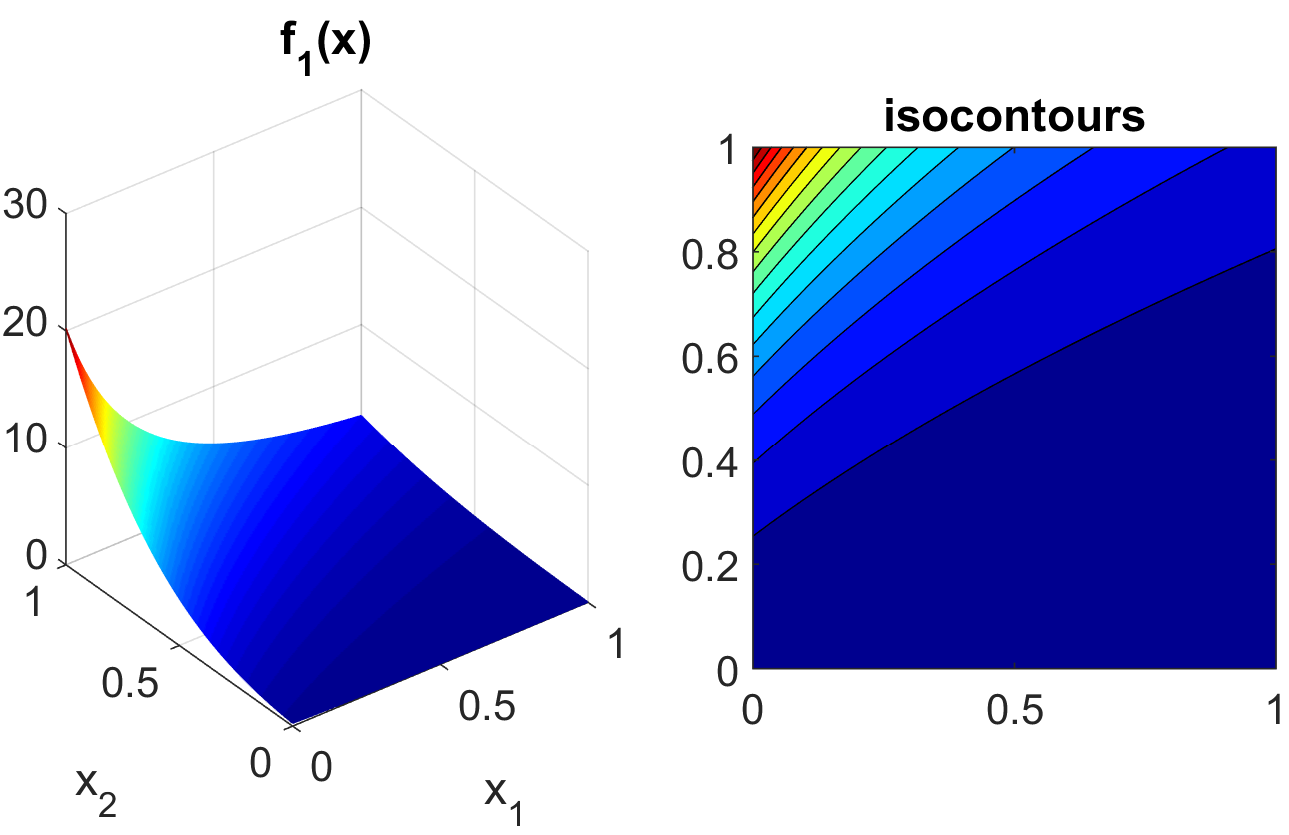
\includegraphics[scale=0.7]{images/sobol_rational}
  \caption{Plot of the \texttt{sobol\_rational} test function in 2 dimensions.}
  \label{fig:sobol_rational}
\end{figure}

The Ishigami test problem~\cite{storlie_09} is a
smooth $C^{\infty}$ function:
\begin{equation}
f({\bf x}) = \sin(2 \pi x_1 - \pi) + 7 \sin^2(2 \pi x_2 - \pi) 
+ 0.1(2 \pi x_3 - \pi)^4 \sin(2 \pi x_1 - \pi)
\end{equation}
where the distributions for $x_1$, $x_2$, and $x_3$ are {\it iid}
uniform on [0,1].  This function was created as a test for global
sensitivity analysis methods, but is challenging for any method based
on low-order structured grids (e.g., due to term cancellation at
midpoints and bounds). 
This function in shown in Figure~\ref{fig:sobol_ishigami}.
\begin{figure}
  \centering
  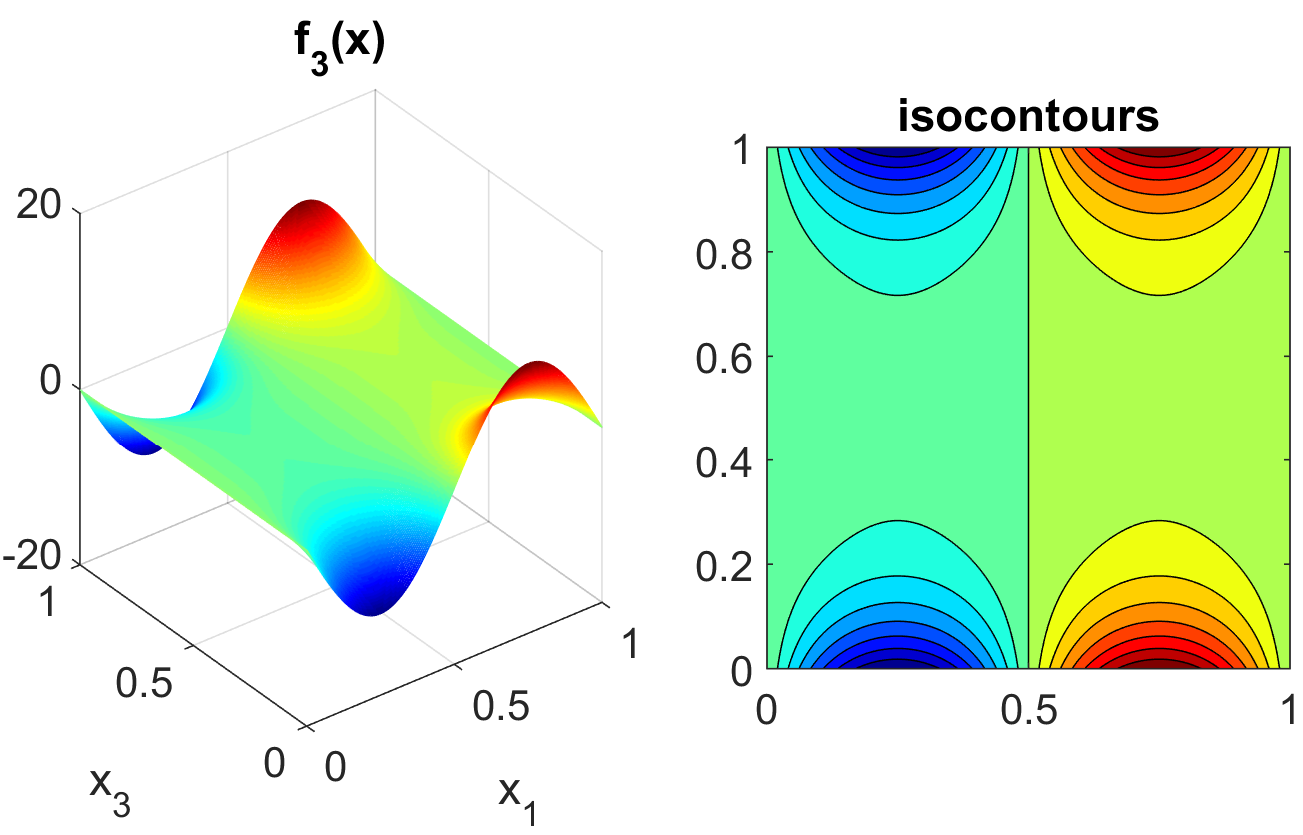
\includegraphics[scale=0.7]{images/sobol_ishigami}
  \caption{Plot of the \texttt{sobol\_ishigami} test function as a function of x1 and x3.}
  \label{fig:sobol_ishigami}
\end{figure}

At the opposite end of the smoothness spectrum, Sobol's
g-function~\cite{storlie_09} is $C^0$ with the absolute value
contributing a slope discontinuity at the center of the domain:
\begin{equation}
f({\bf x}) = 2 \prod_{j=1}^5 \frac{|4x_j - 2| + a_j}{1+a_j};
~~~a = [0, 1, 2, 4, 8]
\end{equation}
The distributions for $x_j$ for $j=1,2,3,4,5$ are {\it iid}
uniform on [0,1]. 
This function in shown in Figure~\ref{fig:sobol_g_function}.
\begin{figure}
  \centering
  \includegraphics[scale=0.7]{images/sobol_g_function}
  \caption{Plot of the \texttt{sobol\_g\_function} test function.}
  \label{fig:sobol_g_function}
\end{figure}


%\clearpage
\section{Cylinder Head}\label{additional:cylinder}

The cylinder head test problem is stated as:
\begin{eqnarray}
\texttt{minimize }   & & f=-1\bigg(\frac{\mathtt{horsepower}}{250}+
  \frac{\mathtt{warranty}}{100000}\bigg) \nonumber\\
\texttt{subject to } & & \sigma_{max} \leq 0.5 \sigma_{yield}
  \label{additional:cylhead}\\
                     & & \mathtt{warranty} \geq 100000          \nonumber\\
                     & & \mathtt{time_{cycle}} \leq 60          \nonumber\\
                     & & 1.5 \leq \mathtt{d_{intake}} \leq 2.164\nonumber\\
                     & & 0.0 \leq \mathtt{flatness} \leq 4.0    \nonumber
\end{eqnarray}

This formulation seeks to simultaneously maximize normalized engine
horsepower and engine warranty over variables of valve intake diameter
($\mathtt{d_{intake}}$) in inches and overall head flatness
($\mathtt{flatness}$) in thousandths of an inch subject to inequality
constraints that the maximum stress cannot exceed half of yield, that
warranty must be at least 100000 miles, and that manufacturing cycle
time must be less than 60 seconds. Since the constraints involve
different scales, they should be nondimensionalized (note: the
nonlinear constraint scaling described in
Section~\ref{opt:additional:scaling} can now do this
automatically). In addition, they can be converted to the standard
1-sided form $g(\mathbf{x}) \leq 0$ as follows:
\begin{eqnarray}
  & & g_1=\frac{2\sigma_{\mathtt{max}}}{\sigma_{\mathtt{yield}}}-1 \leq 0
  \nonumber\\
  & & g_2=1-\frac{\mathtt{warranty}}{100000} \leq 0
  \label{additional:cylheadaltg}\\
  & & g_3=\frac{\mathtt{time_{cycle}}}{60}-1 \leq 0\nonumber
\end{eqnarray}

The objective function and constraints are related analytically to the
design variables according to the following simple expressions:
\begin{eqnarray}
\mathtt{warranty}     &=& 100000+15000(4-\mathtt{flatness})\nonumber\\
\mathtt{time_{cycle}} &=& 45+4.5(4-\mathtt{flatness})^{1.5}\nonumber\\
\mathtt{horsepower}   &=& 250+200\bigg(\frac{\mathtt{d_{intake}}}{1.833}-1\bigg)
  \label{additional:cylheadexp}\\
\sigma_{\mathtt{max}} &=& 750+\frac{1}{(\mathtt{t_{wall}})^{2.5}}\nonumber\\
\mathtt{t_{wall}}     &=& \mathtt{offset_{intake}-offset_{exhaust}}-
  \frac{(\mathtt{d_{intake}+d_{exhaust}})}{2}\nonumber
\end{eqnarray}

where the constants in Equation~\ref{additional:cylheadaltg} and
Equation~\ref{additional:cylheadexp} assume the following values:
$\sigma_{\mathtt{yield}}=3000$,\\$\mathtt{offset_{intake}}=3.25$,
$\mathtt{offset_{exhaust}}=1.34$, and $\mathtt{d_{exhaust}}=1.556$.

\subsection{Constrained Gradient Based Optimization}

An example using the cylinder head test problem is shown below:
\begin{figure}[ht!]
  \centering
  \begin{small}
    \begin{bigbox}
      \verbatimtabinput[8]{../../test/examples-users/cylhead_opt_npsol.in}
    \end{bigbox}
  \end{small}
  \caption{Cylinder Head Example: the Dakota input file --
see \protect\path{dakota/share/dakota/examples/users/cylhead_opt_npsol.in} }
  \label{additional:cylinder_head}
\end{figure}

The interface keyword specifies use of the \texttt{cyl\_head}
executable (compiled from \path{dakota_source/test/cyl_head.cpp}) as the
simulator. The variables and responses keywords specify the data sets
to be used in the iteration by providing the initial point,
descriptors, and upper and lower bounds for two continuous design
variables and by specifying the use of one objective function, three
inequality constraints, and numerical gradients in the problem. The
method keyword specifies the use of the \texttt{npsol\_sqp} method to
solve this constrained optimization problem. No environment keyword is
specified, so the default \texttt{single\_method} approach is used.

The solution for the constrained optimization problem is:
\begin{eqnarray*}
    \mathrm{intake\_dia} &=& 2.122 \\
    \mathrm{flatness}    &=& 1.769
\end{eqnarray*}
with
\begin{eqnarray*}
      f^{\ast} &=& -2.461 \\
    g_1^{\ast} &=&  0.0    ~~\mathrm{(active)} \\
    g_2^{\ast} &=& -0.3347 ~~\mathrm{(inactive)} \\
    g_3^{\ast} &=&  0.0    ~~\mathrm{(active)}
\end{eqnarray*}
which corresponds to the following optimal response quantities:
\begin{eqnarray*}
    \mathrm{warranty}        &=& 133472 \\
    \mathrm{cycle\_time}     &=& 60 \\
    \mathrm{wall\_thickness} &=& 0.0707906 \\
    \mathrm{horse\_power}    &=& 281.579 \\
    \mathrm{max\_stress}     &=& 1500
\end{eqnarray*}

The final report from the Dakota output is as follows:
\begin{small}
\begin{verbatim}
    <<<<< Iterator npsol_sqp completed.
    <<<<< Function evaluation summary: 55 total (55 new, 0 duplicate)
    <<<<< Best parameters          =
                          2.1224188322e+00 intake_dia
                          1.7685568331e+00 flatness
    <<<<< Best objective function  =
                         -2.4610312954e+00
    <<<<< Best constraint values   =
                          1.8407497748e-13
                         -3.3471647504e-01
                          0.0000000000e+00
    <<<<< Best data captured at function evaluation 51
    <<<<< Environment execution completed.
    Dakota execution time in seconds:
      Total CPU        =       0.04 [parent =   0.031995, child =   0.008005]
      Total wall clock =   0.232134
\end{verbatim}
\end{small}

\clearpage
\section{Container}\label{additional:container}

For this example, suppose that a high-volume manufacturer of light
weight steel containers wants to minimize the amount of raw sheet
material that must be used to manufacture a 1.1 quart
cylindrical-shaped can, including waste material. Material for the
container walls and end caps is stamped from stock sheet material of
constant thickness. The seal between the end caps and container wall
is manufactured by a press forming operation on the end caps. The end
caps can then be attached to the container wall forming a seal through
a crimping operation.

\begin{figure}[hb]
  \centering
  \includegraphics[scale=0.4]{images/end_cap}
  \caption{Container wall-to-end-cap seal}
  \label{additional:figure01}
\end{figure}

For preliminary design purposes, the extra material that would
normally go into the container end cap seals is approximated by
increasing the cut dimensions of the end cap diameters by 12\% and the
height of the container wall by 5\%, and waste associated with
stamping the end caps in a specialized pattern from sheet stock is
estimated as 15\% of the cap area. The equation for the area of the
container materials including waste is

\[
A=2 \times \left(\begin{array}{c}
    \mathtt{end\hbox{ }cap}\\
    \mathtt{waste}\\
    \mathtt{material}\\
    \mathtt{factor}
  \end{array} \right)
\times \left(\begin{array}{c}
    \mathtt{end\hbox{ }cap}\\
    \mathtt{seal}\\
    \mathtt{material}\\
    \mathtt{factor}
  \end{array} \right)
\times \left(\begin{array}{c}
    \mathtt{nominal}\\
    \mathtt{end\hbox{ }cap}\\
    \mathtt{area}
  \end{array} \right)
+ \left(\begin{array}{c}
    \mathtt{container}\\
    \mathtt{wall\hbox{ }seal}\\
    \mathtt{material}\\
    \mathtt{factor}
  \end{array} \right)
\times \left(\begin{array}{c}
    \mathtt{nominal}\\
    \mathtt{container}\\
    \mathtt{wall\hbox{ }area}
  \end{array} \right)
\]

or
\begin{equation}
A=2(1.15)(1.12)\pi\frac{D^2}{4}+(1.05)\pi DH \label{additional:contA}
\end{equation}

where $D$ and $H$ are the diameter and height of the finished product
in units of inches, respectively. The volume of the finished product
is specified to be
\begin{equation}
  V=\pi\frac{D^2H}{4}=(1.1\mathtt{qt})(57.75 \mathtt{in}^3/\mathtt{qt})
  \label{additional:contV}
\end{equation}

The equation for area is the objective function for this problem; it
is to be minimized. The equation for volume is an equality constraint;
it must be satisfied at the conclusion of the optimization problem.
Any combination of $D$ and $H$ that satisfies the volume constraint is
a \textbf{feasible} solution (although not necessarily the optimal
solution) to the area minimization problem, and any combination that
does not satisfy the volume constraint is an \textbf{infeasible}
solution. The area that is a minimum subject to the volume constraint
is the \textbf{optimal} area, and the corresponding values for the
parameters $D$ and $H$ are the optimal parameter values.

It is important that the equations supplied to a numerical
optimization code be limited to generating only physically realizable
values, since an optimizer will not have the capability to
differentiate between meaningful and nonphysical parameter values. It
is often up to the engineer to supply these limits, usually in the
form of parameter bound constraints. For example, by observing the
equations for the area objective function and the volume constraint,
it can be seen that by allowing the diameter, $D$, to become negative,
it is algebraically possible to generate relatively small values for
the area that also satisfy the volume constraint. Negative values for
$D$ are of course physically meaningless. Therefore, to ensure that
the numerically-solved optimization problem remains meaningful, a
bound constraint of $-D \leq 0$ must be included in the optimization
problem statement. A positive value for $H$ is implied since the
volume constraint could never be satisfied if $H$ were negative.
However, a bound constraint of $-H \leq 0$ can be added to the
optimization problem if desired. The optimization problem can then be
stated in a standardized form as
\begin{eqnarray}
\texttt{minimize}   & & 2(1.15)(1.12)\pi\frac{D^2}{4}+(1.05)^2\pi DH\nonumber\\
\texttt{subject to} & & \pi\frac{D^2H}{4}=
  (1.1\mathtt{qt})(57.75 \mathtt{in}^3/\mathtt{qt}) \label{additional:contFH}\\
                    & & -D \leq 0\hbox{, }-H \leq 0\nonumber
\end{eqnarray}

A graphical view of the container optimization test problem appears in
Figure~\ref{additional:figure02}. The 3-D surface defines the area,
$A$, as a function of diameter and height. The curved line that
extends across the surface defines the areas that satisfy the volume
equality constraint, $V$. Graphically, the container optimization
problem can be viewed as one of finding the point along the constraint
line with the smallest 3-D surface height in
Figure~\ref{additional:figure02}. This point corresponds to the
optimal values for diameter and height of the final product.

\begin{figure}
  \centering
  \includegraphics[scale=0.3]{images/graphical_container_opt}
  \caption{A graphical representation of the container optimization
    problem.}
  \label{additional:figure02}
\end{figure}

\subsection{Constrained Gradient Based Optimization}

The input file for this example is named
\path{container_opt_npsol.in}. The solution to this example
problem is $(H,D)=(4.99,4.03)$, with a minimum area of 98.43
$\mathtt{in}^2$ .

The final report from the Dakota output is as follows:
\begin{small}
\begin{verbatim}
    <<<<< Iterator npsol_sqp completed.
    <<<<< Function evaluation summary: 40 total (40 new, 0 duplicate)
    <<<<< Best parameters          =
                          4.9873894231e+00 H
                          4.0270846274e+00 D
    <<<<< Best objective function  =
                          9.8432498116e+01
    <<<<< Best constraint values   =
                         -9.6301439045e-12
    <<<<< Best data captured at function evaluation 36
    <<<<< Environment execution completed.
    Dakota execution time in seconds:
      Total CPU        =      0.18 [parent =      0.18, child =         0]
      Total wall clock =  0.809126
\end{verbatim}
\label{cont_opt_npsol.out}
\end{small}

% Begin UQ testers

\section{Cantilever}\label{additional:cantilever}

This test problem is adapted from the reliability-based design
optimization literature~\cite{Sue01},~\cite{Wu01} and involves a simple
uniform cantilever beam as shown in Figure~\ref{additional:figure03}.

\begin{figure}[hbp]
  \centering
  \includegraphics[scale=0.5]{images/cantilever_beam}
  \caption{Cantilever beam test problem.}
  \label{additional:figure03}
\end{figure}

The design problem is to minimize the weight (or, equivalently, the
cross-sectional area) of the beam subject to a displacement constraint
and a stress constraint. Random variables in the problem include the
yield stress $R$ of the beam material, the Young's modulus $E$ of the
material, and the horizontal and vertical loads, $X$ and $Y$, which
are modeled with normal distributions using $N(40000, 2000)$,
$N(2.9E7, 1.45E6)$, $N(500, 100)$, and $N(1000, 100)$, respectively.
Problem constants include $L = 100\mathtt{in}$ and $D_{0} = 2.2535
\mathtt{in}$. The constraints have the following analytic form:
\begin{eqnarray}
\mathtt{stress}&=&\frac{600}{w t^2}Y+\frac{600}{w^2t}X \leq R
  \label{additional:cant}\\
\mathtt{displacement}&=&\frac{4L^3}{E w t}
  \sqrt{\bigg(\frac{Y}{t^2}\bigg)^2+\bigg(\frac{X}{w^2}\bigg)^2}
  \leq D_{0} \nonumber
\end{eqnarray}
or when scaled:
\begin{eqnarray}
  g_{S}&=&\frac{\mathtt{stress}}{R}-1 \leq 0\label{additional:cantscale}\\
  g_{D}&=&\frac{\mathtt{displacement}}{D_{0}}-1 \leq 0\nonumber\\
\end{eqnarray}

{\bf Deterministic Formulation } \\
If the random variables $E$, $R$, $X$, and $Y$ are fixed at their
means, the resulting deterministic design problem can be formulated as
\begin{eqnarray}
\texttt{minimize }   & & f = w t            \nonumber\\
\texttt{subject to } & & g_{S} \leq 0 \label{additional:cantopt}\\
                     & & g_{D} \leq 0       \nonumber\\
                     & & 1.0 \leq w \leq 4.0\nonumber\\
                     & & 1.0 \leq t \leq 4.0\nonumber
\end{eqnarray}

{\bf Stochastic Formulation } \\
If the normal distributions for the random variables $E$, $R$, $X$,
and $Y$ are included, a stochastic design problem can be formulated as
\begin{eqnarray}
\texttt{minimize }   & & f = w t            \nonumber\\
\texttt{subject to } & & \beta_{D} \geq 3   \label{additional:cantouu}\\
                     & & \beta_{S} \geq 3   \nonumber\\
                     & & 1.0 \leq w \leq 4.0\nonumber\\
                     & & 1.0 \leq t \leq 4.0\nonumber
\end{eqnarray}
where a 3-sigma reliability level (probability of failure = 0.00135 if
responses are normally-distributed) is being sought on the scaled
constraints.

\subsection{Constrained Gradient Based Optimization}
The test problem is solved using \path{cantilever_opt_npsol.in}:
\begin{figure}[ht!]
  \centering
  \begin{small}
    \begin{bigbox}
      \verbatimtabinput[8]{../../test/examples-users/cantilever_opt_npsol.in}
    \end{bigbox}
  \end{small}
  \caption{Cantilever Example: the Dakota input file --
see \protect\path{dakota/share/dakota/examples/users/cantilever_opt_npsol.in} }
  \label{additional:cant_opt_npsol}
\end{figure}

The deterministic solution is $(w,t)=(2.35,3.33)$ with an objective
function of $7.82$. The final report from the Dakota output is as
follows:
\begin{small}
\begin{verbatim}
    <<<<< Iterator npsol_sqp completed.
    <<<<< Function evaluation summary: 33 total (33 new, 0 duplicate)
    <<<<< Best parameters          =
                          2.3520341271e+00 beam_width
                          3.3262784077e+00 beam_thickness
                          4.0000000000e+04 R
                          2.9000000000e+07 E
                          5.0000000000e+02 X
                          1.0000000000e+03 Y
    <<<<< Best objective function  =
                          7.8235203313e+00
    <<<<< Best constraint values   =
                         -1.6009000260e-02
                         -3.7083558446e-11
    <<<<< Best data captured at function evaluation 31
    <<<<< Environment execution completed.
    Dakota execution time in seconds:
      Total CPU        =       0.03 [parent =   0.027995, child =   0.002005]
      Total wall clock =   0.281375
\end{verbatim}
\end{small}

\subsection{Optimization Under Uncertainty}
Optimization under uncertainty solutions to the
stochastic problem are described in~\cite{Eld02,Eld05,Eld06a}, for
which the solution is $(w,t)=(2.45,3.88)$ with an objective function
of $9.52$. This demonstrates that a more conservative design is
needed to satisfy the probabilistic constraints.

\section{Multiobjective Test Problems}\label{additional:multiobjective}

Multiobjective optimization means that there are two or more
objective functions that you wish to optimize simultaneously. Often
these are conflicting objectives, such as cost and performance. The
answer to a multi-objective problem is usually not a single point.
Rather, it is a set of points called the Pareto front. Each point
on the Pareto front satisfies the Pareto optimality criterion, i.e.,
locally there exists no other feasible vector that would improve some
objective without causing a simultaneous worsening in at least one
other objective. Thus a feasible point $X^\prime$ from which
small moves improve one or more objectives without worsening
any others is not Pareto optimal: it is said to be ``dominated''
and the points along the Pareto front are said to be
``non-dominated''.

Often multi-objective problems are addressed by simply assigning
weights to the individual objectives, summing the weighted objectives,
and turning the problem into a single-objective one which can be
solved with a variety of optimization techniques. While this approach
provides a useful ``first cut'' analysis (and is supported within
Dakota---see Section~\ref{opt:additional:multiobjective}), this
approach has many limitations. The major limitation is that a local
solver with a weighted sum objective will only find one
% optimal solutions if the true Pareto front is nonconvex. %Hogwash!
point on the Pareto front; if one wants to understand
the effects of changing weights, this method can be computationally
expensive. Since each optimization of a single weighted objective
will find only one point on the Pareto front, many
optimizations must be performed to get a good parametric
understanding of the influence of the weights and to achieve a good
sampling of the entire Pareto frontier.

There are three examples that are taken from a multiobjective
evolutionary algorithm (MOEA) test suite described by Van Veldhuizen
et. al. in~\cite{Coe02}. These three examples illustrate the different
forms that the Pareto set may take. For each problem, we describe the
Dakota input and show a graph of the Pareto front. These problems are
all solved with the \texttt{moga} method.  The first example is
discussed in Section~\ref{opt:additional:multiobjective}.  The next
two are discussed below.  Section~\ref{opt:additional:multiobjective}
provide more information on multiobjective optimization.

\subsection{Multiobjective Test Problem 2}\label{additional:multiobjective:problem2}

The second test problem is a case where both $\mathtt{P_{true}}$ and
$\mathtt{PF_{true}}$ are disconnected. $\mathtt{PF_{true}}$ has four
separate Pareto curves. The problem is to simultaneously optimize
$f_1$ and $f_2$ given two input variables, $x_1$ and $x_2$,
where the inputs are bounded by $0 \leq x_{i} \leq 1$, and:
\begin{eqnarray*}
f_1(x) &=& x_1 \\
f_2(x) &=& (1+10x_2) \times \left[1-\bigg(\frac{x_1}{1+10x_2}\bigg)^2-
\frac{x_1}{1+10x_2}\sin(8\pi x_1)\right]
\end{eqnarray*}

The input file for this example is shown in
Figure~\ref{additional:moga2inp}, which references the
\texttt{mogatest2} executable (compiled from
\path{dakota_source/test/mogatest2.cpp}) as the simulator. The Pareto
front is shown in Figure~\ref{additional:moga2front}. Note the
discontinuous nature of the front in this example.

\begin{figure}
  \centering
  \begin{bigbox}
    \begin{small}
      \verbatimtabinput[8]{../../test/examples-users/mogatest2.in}
    \end{small}
  \end{bigbox}
  \caption{Dakota input file specifying the use of MOGA on mogatest2 --
see \protect\path{dakota/share/dakota/examples/users/mogatest2.in} }
  \label{additional:moga2inp}
\end{figure}

\begin{figure}
  \centering
  \includegraphics[scale=0.75]{images/dakota_mogatest2_pareto_front}
  \caption{Pareto Front showing Tradeoffs between Function F1 and
    Function F2 for mogatest2}
  \label{additional:moga2front}
\end{figure}

\subsection{Multiobjective Test Problem 3}\label{additional:multiobjective:problem3}

The third test problem is a case where $\mathtt{P_{true}}$ is
disconnected but $\mathtt{PF_{true}}$ is connected.
% It is called the Srinivas problem in the literature (cite).
This problem also has two
nonlinear constraints. The problem is to simultaneously optimize
$f_1$ and $f_2$ given two input variables, $x_1$ and $x_2$,
where the inputs are bounded by $-20 \leq x_{i} \leq 20$, and:
\begin{eqnarray*}
f_1(x) &=& (x_1-2)^2+(x_2-1)^2+2 \\
f_2(x) &=& 9x_1-(x_2-1)^2
\end{eqnarray*}

The constraints are:
\begin{eqnarray*}
0 &\leq& x_1^2+x_2^2-225 \\
0 &\leq& x_1-3x_2+10
\end{eqnarray*}

The input file for this example is shown in
Figure~\ref{additional:moga3inp}. It differs from
Figure~\ref{additional:moga2inp} in the variables and responses
specifications, in the use of the \texttt{mogatest3} executable
(compiled from \path{dakota_source/test/mogatest3.cpp}) as the simulator, and
in the \texttt{max\_function\_evaluations} and \texttt{mutation\_type}
MOGA controls. The Pareto set is shown in
Figure~\ref{additional:moga3set}. Note the discontinuous nature of the
Pareto set (in the design space) in this example. The Pareto front is
shown in Figure~\ref{additional:moga3front}.
%Again, note the unusual nature of this Pareto example (these figures
%agree reasonably well with the Srinivas problem results shown in the
%literature).

\begin{figure}
  \centering
  \begin{bigbox}
    \begin{small}
      \verbatimtabinput[8]{../../test/examples-users/mogatest3.in}
    \end{small}
  \end{bigbox}
  \caption{Dakota input file specifying the use of MOGA on mogatest3 --
see \protect\path{dakota/share/dakota/examples/users/mogatest3.in} }
  \label{additional:moga3inp}
\end{figure}

\begin{figure}
  \centering
  \includegraphics[scale=0.75]{images/dakota_mogatest3_pareto_set}
  \caption{Pareto Set of Design Variables corresponding to the Pareto
    front for mogatest3}
  \label{additional:moga3set}
\end{figure}

\begin{figure}
  \centering
  \includegraphics[scale=0.75]{images/dakota_mogatest3_pareto_front}
  \caption{Pareto Front showing Tradeoffs between Function F1 and
    Function F2 for mogatest3}
  \label{additional:moga3front}
\end{figure}

\clearpage
\section{Morris}\label{additional:morris}

Morris~\cite{Mor91} includes a screening design test problem with a
single-output analytical test function. The output depends on 20
inputs with first- through fourth-order interaction terms, some having
large fixed coefficients and others small random coefficients. Thus
the function values generated depend on the random number generator
employed in the function evaluator. The computational model is:

\begin{align*}
y = &\;\beta_0 + \sum_{i=1}^{20}{\beta_i w_i} + \sum_{i<j}^{20}{\beta_{i,j} w_i w_j} + \sum_{i<j<l}^{20}{\beta_{i,j,l} w_i w_j w_l} \\
    &+  \sum_{i<j<l<s}^{20}{\beta_{i,j,l,s} w_i w_j w_l w_s},
\end{align*}
where $w_i = 2(x_i-0.5)$ except for $i=3, 5, \mbox{ and } 7$, where $w_i=2(1.1x_i/(x_i+0.1) - 0.5)$. Large-valued coefficients are assigned as
\begin{align*}
&\beta_i = +20 & &i=1,\ldots,10; \;&\beta_{i,j} = -15& &i,j = 1, \ldots, 6; \\
&\beta_{i,j,l} = -10& &i,j,l=1,\ldots,5; \;&\beta_{i,j,l,s} = +5& &i,j,l,s = 1, \ldots, 4.
\end{align*}
The remaining first- and second-order coefficients $\beta_i$ and
$\beta_{i,j}$, respectively, are independently generated from a
standard normal distribution (zero mean and unit standard deviation);
the remaining third- and fourth-order coefficients are set to zero.

Examination of the test function reveals that one should be able to
conclude the following (stated and verified computationally
in~\cite{Sal04}) for this test problem:
\begin{enumerate}
\item the first ten factors are important;
\item of these, the first seven have significant effects involving
      either interactions or curvatures; and
\item the other three are important mainly because of their first-order
      effect.
\end{enumerate}

\subsection{Morris One-at-a-Time Sensitivity Study}

The dakota input \path{morris_ps_moat.in} exercises
the MOAT algorithm described in Section~\ref{dace:psuade} on the
Morris problem. The Dakota output obtained is shown in
Figures~\ref{FIG:moat:out_preamble} and~\ref{FIG:moat:out_results}.
\begin{figure}[ht!]
\centering
\begin{bigbox}
\begin{small}
\begin{verbatim}
Running MPI executable in serial mode.
Dakota version 6.0 release.
Subversion revision xxxx built May ...
Writing new restart file dakota.rst
gradientType = none
hessianType = none

>>>>> Executing environment.

>>>>> Running psuade_moat iterator.

PSUADE DACE method = psuade_moat Samples = 84 Seed (user-specified) = 500
            Partitions = 3 (Levels = 4)
\end{verbatim}
\end{small}
\end{bigbox}
\caption[Dakota initialization output for PSUADE
MOAT.]{\label{FIG:moat:out_preamble} Dakota initialization output for
the PSUADE MOAT method on the Morris test problem showing the study
parameters.}
\end{figure}
\begin{figure}[ht!]
\centering
\begin{bigbox}
\begin{small}
\begin{verbatim}
>>>>>> PSUADE MOAT output for function 0:

*************************************************************
*********************** MOAT Analysis ***********************
-------------------------------------------------------------
Input   1 (mod. mean & std) =   9.5329e+01   9.0823e+01
Input   2 (mod. mean & std) =   6.7297e+01   9.5242e+01
Input   3 (mod. mean & std) =   1.0648e+02   1.5479e+02
Input   4 (mod. mean & std) =   6.6231e+01   7.5895e+01
Input   5 (mod. mean & std) =   9.5717e+01   1.2733e+02
Input   6 (mod. mean & std) =   8.0394e+01   9.9959e+01
Input   7 (mod. mean & std) =   3.2722e+01   2.7947e+01
Input   8 (mod. mean & std) =   4.2013e+01   7.6090e+00
Input   9 (mod. mean & std) =   4.1965e+01   7.8535e+00
Input  10 (mod. mean & std) =   3.6809e+01   3.6151e+00
Input  11 (mod. mean & std) =   8.2655e+00   1.0311e+01
Input  12 (mod. mean & std) =   4.9299e+00   7.0591e+00
Input  13 (mod. mean & std) =   3.5455e+00   4.4025e+00
Input  14 (mod. mean & std) =   3.4151e+00   2.4905e+00
Input  15 (mod. mean & std) =   2.5143e+00   5.5168e-01
Input  16 (mod. mean & std) =   9.0344e+00   1.0115e+01
Input  17 (mod. mean & std) =   6.4357e+00   8.3820e+00
Input  18 (mod. mean & std) =   9.1886e+00   2.5373e+00
Input  19 (mod. mean & std) =   2.4105e+00   3.1102e+00
Input  20 (mod. mean & std) =   5.8234e+00   7.2403e+00
<<<<< Function evaluation summary: 84 total (84 new, 0 duplicate)
\end{verbatim}
\end{small}
\end{bigbox}
\caption[Dakota analysis output for PSUADE
MOAT.]{\label{FIG:moat:out_results} Dakota analysis output for the
PSUADE MOAT method on the Morris problem showing the modified
mean and standard deviation of the elementary effect corresponding to
each input factor.}
\end{figure}
The MOAT analysis output reveals that each of the desired observations
can be made for the test problem. These are also reflected in
Figure~\ref{FIG:mustar_sigma}. The modified mean (based on averaging
absolute values of elementary effects) shows a clear difference in
inputs 1--10 as compared to inputs 11--20. The standard deviation of
the (signed) elementary effects indicates correctly that inputs 1--7
have substantial interaction-based or nonlinear effect on the output,
while the others have less. While some of inputs 11--20 have
nontrivial values of $\sigma$, their relatively small modified means
$\mu^*$ indicate they have little overall influence.

\begin{figure}[ht!]
\centering
\includegraphics[width=\textwidth]{images/moat_mustar_sigma}
\caption{\label{FIG:mustar_sigma} Standard deviation of elementary
effects plotted against modified mean for Morris for each of 20
inputs. Red circles 1--7 correspond to inputs having interactions or
nonlinear effects, blue squares 8--10 indicate those with mainly
linear effects, and black Xs denote insignificant inputs.}
\end{figure}

\clearpage
\section{Test Problems for Reliability Analyses}\label{additional:reliabilityproblems}
This section includes several test problems and examples related to
reliability analyses. {\bf These are NOT included in the
  \path{dakota/share/dakota/examples/users} directory, but are in the
  \path{dakota/share/dakota/test} directory.}


\subsection{Log Ratio}\label{additional:logratio}

This test problem, mentioned previously in
Section~\ref{uq:reliability:ex}, has a limit state function defined by
the ratio of two lognormally-distributed random variables.
\begin{equation}
g({\bf x}) = \frac{x_1}{x_2}
\end{equation}
The distributions for both $x_1$ and $x_2$ are Lognormal(1, 0.5) with
a correlation coefficient between the two variables of 0.3.

{\bf Reliability Analyses} \\

First-order and second-order reliability analysis (FORM and SORM) are performed in the
\path{logratio_uq_reliability.in} in the \path{dakota/share/dakota/examples/users}
 directory and \path{dakota_logratio_taylor2.in} in directory
\path{dakota/share/dakota/test}.

For the reliability index approach (RIA),
24 response levels (.4, .5, .55,
.6, .65, .7, .75, .8, .85, .9, 1, 1.05, 1.15, 1.2, 1.25, 1.3, 1.35,
1.4, 1.5, 1.55, 1.6, 1.65, 1.7, and 1.75) are mapped into the
corresponding cumulative probability levels. For performance measure approach (PMA), these 24
probability levels (the fully converged results from RIA FORM) are
mapped back into the original response levels.
Figure~\ref{fig:log_ratio_cdf} overlays the computed CDF values for a
number of first-order reliability method variants as well as a Latin
Hypercube reference solution of $10^6$ samples.
\begin{figure}[hbp]
\centering
\centerline{\includegraphics[scale=0.5]{images/log_ratio_cdf_ria}
            \includegraphics[scale=0.5]{images/log_ratio_cdf_pma}}
(a) RIA methods\hspace{2.5in}(b) PMA methods
\caption{Lognormal ratio cumulative distribution function, RIA/PMA methods.}
\label{fig:log_ratio_cdf}
\end{figure}

\subsection{Steel Section}\label{additional:steel_section}

This test problem is used extensively in~\cite{Hal00}. It involves a
W16x31 steel block of A36 steel that must carry an applied
deterministic bending moment of 1140 kip-in. For Dakota, it has been
used as a code verification test for second-order integrations in
reliability methods. The limit state function is defined as:
\begin{equation}
g({\bf x}) = F_y Z - 1140
\end{equation}
where $F_y$ is Lognormal(38., 3.8), $Z$ is Normal(54., 2.7), and the
variables are uncorrelated.

The \path{dakota/share/dakota/test/dakota_steel_section.in} input file computes
a first-order CDF probability of $p(g \leq 0.)$ = 1.297e-07 and a
second-order CDF probability of $p(g \leq 0.)$ = 1.375e-07. This
second-order result differs from that reported in~\cite{Hal00}, since
Dakota uses the Nataf nonlinear transformation to u-space (see MPP
Search Methods block in Reliability Methods chapter of Dakota Theory
Manual~\cite{TheoMan}) and \cite{Hal00} uses a linearized
transformation.

\subsection{Portal Frame}\label{additional:portal_frame}


This test problem is taken from~\cite{Tve90,Hon99}. It involves a
plastic collapse mechanism of a simple portal frame. It also has been
used as a verification test for second-order integrations in
reliability methods. The limit state function is defined as:
\begin{equation}
g({\bf x}) = x_1 + 2 x_2 + 2 x_3 + x_4 - 5 x_5 - 5 x_6
\end{equation}
where $x_1 - x_4$ are Lognormal(120., 12.), $x_5$ is Lognormal(50.,
15.), $x_6$ is Lognormal(40., 12.), and the variables are uncorrelated.

While the limit state is linear in x-space, the nonlinear
transformation of lognormals to u-space induces curvature. The
\path{dakota/share/dakota/test/dakota_portal_frame.in} input file computes a
first-order CDF probability of $p(g \leq 0.)$ = 9.433e-03 and a
second-order CDF probability of $p(g \leq 0.)$ = 1.201e-02. These
results agree with the published results from the literature.

\subsection{Short Column}\label{additional:short_column}

This test problem involves the plastic analysis and design of a short
column with rectangular cross section (width $b$ and depth $h$) having
uncertain material properties (yield stress $Y$) and subject to
uncertain loads (bending moment $M$ and axial force $P$)~\cite{Kus97}.
The limit state function is defined as:
\begin{equation}
g({\bf x}) = 1 - \frac{4M}{b h^2 Y} - \frac{P^2}{b^2 h^2 Y^2}
\end{equation}

The distributions for $P$, $M$, and $Y$ are Normal(500, 100),
Normal(2000, 400), and Lognormal(5, 0.5), respectively, with a
correlation coefficient of 0.5 between $P$ and $M$ (uncorrelated
otherwise). The nominal values for $b$ and $h$ are 5 and 15,
respectively.

{\bf Reliability Analyses} \\

First-order and second-order reliability analysis are performed in the
\path{dakota_short_column.in} and
\path{dakota_short_column_taylor2.in} input files in
\path{dakota/share/dakota/test}. For RIA, 43 response levels (-9.0, -8.75,
-8.5, -8.0, -7.75, -7.5, -7.25, -7.0, -6.5, -6.0, -5.5, -5.0, -4.5,
-4.0, -3.5, -3.0, -2.5, -2.0, -1.9, -1.8, -1.7, -1.6, -1.5, -1.4,
-1.3, -1.2, -1.1, -1.0, -0.9, -0.8, -0.7, -0.6, -0.5, -0.4, -0.3,
-0.2, -0.1, 0.0, 0.05, 0.1, 0.15, 0.2, 0.25) are mapped into the
corresponding cumulative probability levels. For PMA, these 43
probability levels (the fully converged results from RIA FORM) are
mapped back into the original response levels.
Figure~\ref{fig:short_col_cdf} overlays the computed CDF values for
several first-order reliability method variants as well as a Latin
Hypercube reference solution of $10^6$ samples.

\begin{figure}
\centering
\centerline{\includegraphics[scale=0.5]{images/short_col_cdf_ria}
            \includegraphics[scale=0.5]{images/short_col_cdf_pma}}
(a) RIA methods\hspace{2.75in}(b) PMA methods
\caption{Short column cumulative distribution function, RIA/PMA methods.}
\label{fig:short_col_cdf}
\end{figure}

{\bf Reliability-Based Design Optimization} \\

The short column test problem is also amenable to Reliability-Based Design Optimization (RBDO). An
objective function of cross-sectional area and a target reliability
index of 2.5 (cumulative failure probability $p(g \le 0) \le 0.00621$)
are used in the design problem:
\begin{eqnarray}
\min       & & bh \nonumber \\
{\rm s.t.} & & \beta \geq 2.5 \nonumber \\
           & &  5.0 \leq b \leq 15.0 \nonumber \\
           & & 15.0 \leq h \leq 25.0
\end{eqnarray}
As is evident from the UQ results shown in
Figure~\ref{fig:short_col_cdf}, the initial design of $(b, h) = (5,
15)$ is infeasible and the optimization must add material to obtain
the target reliability at the optimal design $(b, h) = (8.68, 25.0)$.
Simple bi-level, fully analytic bi-level, and sequential RBDO methods
are explored in inputs files \path{dakota_rbdo_short_column.in},
\path{dakota_rbdo_short_column_analytic.in}, and
\path{dakota_rbdo_short_column_trsb.in}, with results as described
in~\cite{Eld05,Eld06a}. These files are located in
\path{dakota/share/dakota/test}.

\subsection{Steel Column}\label{additional:steel_column}

This test problem involves the trade-off between cost and
reliability for a steel column~\cite{Kus97}. The cost is defined as
\begin{equation}
Cost = b d + 5 h
\end{equation}
where $b$, $d$, and $h$ are the means of the flange breadth, flange
thickness, and profile height, respectively. Nine uncorrelated random
variables are used in the problem to define the yield stress $F_s$
(lognormal with $\mu/\sigma$ = 400/35 MPa), dead weight load $P_1$
(normal with $\mu/\sigma$ = 500000/50000 N), variable load $P_2$
(gumbel with $\mu/\sigma$ = 600000/90000 N), variable load $P_3$
(gumbel with $\mu/\sigma$ = 600000/90000 N), flange breadth $B$
(lognormal with $\mu/\sigma$ = $b$/3 mm), flange thickness $D$
(lognormal with $\mu/\sigma$ = $d$/2 mm), profile height $H$
(lognormal with $\mu/\sigma$ = $h$/5 mm), initial deflection $F_0$
(normal with $\mu/\sigma$ = 30/10 mm), and Young's modulus $E$ (Weibull
with $\mu/\sigma$ = 21000/4200 MPa). The limit state has the
following analytic form:
\begin{equation}
g = F_s - P \left( \frac{1}{2 B D} +
\frac{F_0}{B D H} \frac{E_b}{E_b - P} \right)\\
\end{equation}
where
\begin{eqnarray}
P   & = & P_1 + P_2 + P_3 \\
E_b & = & \frac{\pi^2 E B D H^2}{2 L^2}
\end{eqnarray}
and the column length $L$ is 7500 mm.

This design problem (\path{dakota_rbdo_steel_column.in} in
\path{dakota/share/dakota/test}) demonstrates design variable insertion into
random variable distribution parameters through the design of the mean
flange breadth, flange thickness, and profile height. The RBDO
formulation maximizes the reliability subject to a cost constraint:
\begin{eqnarray}
{\rm maximize }   & & \beta                   \nonumber \\
{\rm subject to } & & Cost  \leq 4000.       \nonumber \\
                  & & 200.0 \leq b \leq 400.0 \\
                  & &  10.0 \leq d \leq  30.0 \nonumber \\
                  & & 100.0 \leq h \leq 500.0 \nonumber
\end{eqnarray}
which has the solution ($b$, $d$, $h$) = (200.0, 17.50, 100.0) with a
maximal reliability of 3.132.

\section{Test Problems for Forward Uncertainty Quantification}\label{additional:fwd_uq}
This section includes several test problems and examples related to
forward uncertainty quantification. {\bf These are NOT included in the
  \path{dakota/share/dakota/examples/users} directory, but are in the
  \path{dakota/share/dakota/test} directory.}

\subsection{Genz functions}
The Genz functions have traditionally been used to test quadrature
methods, however more recently they hav also been used to test forward
UQ methdos. Here we consider the oscilatory and corner-peak test
functions, respectively given by
\[
 f_{\mathrm{OS}}(\boldsymbol{\xi})=\cos\left(-\sum_{i=1}^d c_i\, \xi_i \right),\quad \boldsymbol{\xi}\in[0,1]^d
\]
\[
 f_{\mathrm{CP}}(\boldsymbol{\xi})=\left(1+\sum_{i=1}^d c_i\, \xi_i \right)^{-(d+1)},\quad \boldsymbol{\xi}\in[0,1]^d
\]
The coefficients $c_k$ can be used to control the effective dimensionality
and the variability of these functions. In dakota we support three
choices of $\boldsymbol = (c_1,\ldots,c_d)^T$, specifically
\[
c^{(1)}_k=\frac{k-\frac{1}{2}}{d},\quad c_k^{(2)}=\frac{1}{k^2}\quad \text{and}
\quad c_k^{(3)} = \exp\left(\frac{k\log(10^{-8})}{d}\right), \quad k=1,\ldots,d
\]
normalizing such that for the oscillatory function $\sum_{k=1}^d c_k =
4.5$ and for the corner peak function $\sum_{k=1}^d c_k = 0.25$. The
different decay rates of the coefficients represent increasing levels
of anisotropy and decreasing effective dimensionality. Anisotropy
refers to the dependence of the function variability.

In Dakota the genz function can be set by specifying
{\tt analysis\_driver='genz'}. The type of coefficients decay can be
set by sepcifying {\tt os1, cp1} which uses $\mathbf{c}^{(1)}$,
{\tt os2, cp2} which uses
$\mathbf{c}^{(2)}$, and {\tt os3, cp3} which uses $\mathbf{c}^{(3)}$,
where {\tt os} is to be used with the oscillatory function and {\tt
 cp} for the corner peak function

\subsection{Elliptic Partial differential equation with uncertain
  coefficients}
Consider the following problem with $d \ge 1$ random dimensions:
\begin{equation}\label{eq:hetrogeneous-diffusion}
-\frac{d}{dx}\left[a(x,\boldsymbol{\xi})\frac{du}{dx}(x,\boldsymbol{\xi})\right] = 10,\quad
(x,\boldsymbol{\xi})\in(0,1)\times I_{\boldsymbol{\xi}}
\end{equation}
subject to the physical boundary conditions
\begin{equation}
u(0,\boldsymbol{\xi})=0,\quad u(1,\boldsymbol{\xi})=0.
\end{equation}
We are interested in quantifying the uncertainty in the solution $u$
at a number of locations $x\in[0,1]$ which can be specified by the
user. This function can be run using dakota by specifying\\
{\tt analysis\_driver='steady\_state\_diffusion\_1d'}.

We represent the random diffusivity field $a$ using two types of
expansions. The first option is to use represent the {\it logarithm} of the
diffusivity field as Karhunen Lo\'{e}ve expansion
\begin{equation}\label{eq:diffusivityZ}
\log(a(x,\boldsymbol{\xi}))=\bar{a}+\sigma_a\sum_{k=1}^d\sqrt{\lambda_k}\phi_k(x)\xi_k
\end{equation}
where $\{\lambda_k\}_{k=1}^d$ and $\{\phi_k(x)\}_{k=1}^d$ are, respectively,
the eigenvalues and eigenfunctions of the covariance kernel
\begin{equation}\label{eq:heat-eq-qoi}
 C_a(x_1,x_2) = \exp\left[-\frac{(x_1-x_2)^p}{l_c}\right].
\end{equation}
for some power $p=1,2$.
The variability of the diffusivity field~\eqref{eq:diffusivityZ} is
controlled by $\sigma_a$ and the correlation length
$l_c$ which determines the decay of the eigenvalues
$\lambda_k$. Dakota sets $\sigma_a=1.$ but allows the number of random
variables $d$, the order of the kernel $p$ and the correlation
length $l_c$ to vary. The random variables can be bounded or unbounded.

The second expansion option is to represent the diffusivity by
\begin{equation}\label{diffusivityZ}
a(x,\boldsymbol{\xi})=1+\sigma\sum_{k=1}^d\frac{1}{k^2\pi^2}\cos(2\pi kx)\boldsymbol{\xi}_k
\end{equation}
where $\boldsymbol{\xi}_k\in[-1,1]$, $k=1,\ldots,d$ are bounded random variables. The form of \eqref{diffusivityZ} is
similar to that obtained from a Karhunen-Lo\`{e}ve expansion. If the
variables are i.i.d. uniform in [-1,1] the the diffusivity satisfies
satisfies the auxiliary properties
\begin{equation}
\mathbb{E}[a(x,\boldsymbol{\xi})]=1\quad\text{and}\quad 1-\frac{\sigma}{6}<a(x,\boldsymbol{\xi})<1+\frac{\sigma}{6}.
\end{equation}
This is the same test case used in \cite{Xiu_Hesthaven_05}.


\subsection{Damped Oscillator}
Consider a damped linear oscillator subject to external forcing
with six unknown parameters $\boldsymbol{\xi}=(\gamma,k,f,\omega,x_0,x_1)$
\begin{equation}\label{eq:oscillator_ode}
\frac{d^2x}{dt^2}(t,\boldsymbol{\xi})+\gamma\frac{dx}{dt}+k x=f\cos(\omega t),
\end{equation}
subject to the initial conditions
\begin{equation}
x(0)=x_0,\quad \dot{x}(0)=x_1,
\end{equation}
Here we assume the damping coefficient $\gamma$, spring constant $k$,
forcing amplitude $f$ and frequency $\omega$, and the initial
conditions $x_0$ and $x_1$ are all uncertain.

This test function can be specified with {\tt
  analysis\_driver='damped\_oscillator'}. This function only works with
the uncertain variables defined over certain ranges. These ranges
are
$$\gamma_k\in[0.08,0.12],k\in[0.03,0.04],f\in[0.08,0.12],\omega\in[0.8,1.2],x_0\in[0.45,0.55],x_1\in[-0.05,0.05].$$
Do not use this function with unbounded variables, however any
bounded variables such as Beta and trucated Normal variables that
satisfy the aforementioned variable bounds are fine.

\subsection{Non-linear coupled system of ODEs}\label{sec:predator-prey}
Consider the non-linear system of ordinary differential equations
governing a competitive Lotka–Volterra model of the population
dynamics of species competing for some common resource. The model is given by
\begin{equation}\label{eq:predprey}
\begin{cases}
\frac{du_i}{dt} = r_iu_i\left(1-\sum_{j=1}^3\alpha_{ij}u_j\right), & \quad t\in (0,10],\\
u_i(0) = u_{i,0}
\end{cases},
\end{equation}
for $i = 1,2,3$.  The initial condition, $u_{i,0}$, and the
self-interacting terms, $\alpha_{ii}$, are given, but the remaining
interaction parameters, $\alpha_{ij}$ with $i\neq j$ as well as the
re-productivity parameters, $r_i$, are unknown.
We approximate the solution to~\eqref{eq:predprey} in time using a
Backward Euler method.

This test function can be specified with {\tt
  analysis\_driver='predator\_prey'}.

We assume that these parameters are bounded. We have tested this model
with all 9 parameters $\xi_i\in[0.3,0.7]$. However larger bounds are
probably valid.  When using the aforemetioned ranges and $1000$ time steps
with $\Delta t = 0.01$ the average (over the random parameters)
deterministic error is approximately $1.00\times10^{-4}$.

Dakota returns the population of each species $u_i(T)$ at the final
time $T$. The final time and the number of time-steps can be changed.

\subsection{Experimental Design}

This example tests the Bayesian experimental design algorithm described in
Section~\ref{sec:bayes_expdesign}, in which a low-fidelity model is calibrated 
to optimally-selected data points of a high-fidelity model. The 
\texttt{analysis\_driver} for the the low and high-fidelity models implement 
the steady state heat example given in~\cite{Lew16}. The high-fidelity model
is the analytic solution to the example described therein,
\begin{equation}
T(x) = c_{1} \exp(-\gamma x) + c_{2} \exp(\gamma x) + T_{amb},
\end{equation}
where
\begin{eqnarray*}
c_{1} &=& - \frac{\Phi}{K \gamma} \left[ \frac{ \exp(\gamma L) (h + K \gamma) }
{\exp(-\gamma L) (h-K\gamma) + \exp(\gamma L) (h+K\gamma)} \right], \\
c_{2} &=& \frac{\Phi}{K\gamma} + c_{1}, \\
\gamma &=& \sqrt{ \frac{ 2(a+b)h }{ abK } }.
\end{eqnarray*}
The ambient room temperature $T_{amb}$, thermal conductivity coefficient $K$, 
convective heat transfer coefficient $h$, source heat flux $\Phi$, and
system dimenions $a$, $b$, and $L$ are all set to constant values. The 
experimental design variable $x \in [10,70]$, is called a configuration variable
in Dakota and is the only variable that also appears in the low-fidelity model,
\begin{equation}
y = A x^2 + B x + C.
\end{equation}
The goal of this example is to calibrate the low-fidelity model parameters
$A, B$, and $C$ with the Bayesian experimental design algorithm. 
Refer to Section~\ref{sec:bayes_expdesign} for further details regarding the
Dakota implementation of this example.

\subsection{Bayes linear}\label{sec:bayes_linear}
This is a simple model that is only available by using the {\tt direct} interface 
with \dakotakw{analysis_driver} {\tt 'bayes\_linear'}.  The model is discussed extensively in 
~\cite{CASL2014} both on pages 93--102 and in Appendix A.  The model is simply the 
sum of the d input parameters: 
\begin{equation}
y = \sum\limits_{i=1}^d x_i
\end{equation}
where the input varaibles $x_i$ can be any uncertain variable type but are typically 
considered as uniform or normal uncertain inputs. 


\bibliographystyle{plain}
\bibliography{Users}

\begin{SANDdistribution}
  % ACADEMIA

  % INDUSTRY

  % LABS

  % SANDIA INTERNAL  
  %\SANDdistInternal{1}{MailStop}{Name}{Organization}
  \SANDdistInternal{10}{1318}{B.~M.~Adams}{1411}

  % Housekeeping copies necessary for every unclassified report:
  \SANDdistInternal{1}{9018}{Central Technical Files}{8940-2}
  \SANDdistInternal{2}{0899}{Technical Library}{4916}
  \SANDdistInternal{2}{0619}{Review \& Approval Desk}{4916}

  % If report has a Patent Caution or Patent Interest, add this:
  %\SANDdistInternal{3}{0161}{Patent and Licensing Office}{4916}
\end{SANDdistribution}

\end{document}
